\documentclass[pra,twocolumn,floatfix,superscriptaddress]{revtex4-1} %reprint
%\tightenlines

%\draft
\usepackage{etex}
\usepackage{amsmath}
\usepackage{bm}
\usepackage{bbm}
\usepackage{listings}
% % \textwidth 16cm \textheight 23.5cm
% \renewcommand{\baselinestretch}{1.2}
\usepackage{graphicx}
\usepackage{graphics}
\usepackage{epsfig}
\usepackage{color}
\usepackage[dvipsnames]{xcolor}
\usepackage{multirow}
\usepackage[colorlinks]{hyperref}
\usepackage{fancyhdr}
\usepackage{calc}
\usepackage{natbib} %[numbers]
\usepackage{bibentry}
\usepackage{bbm}

% todo list and commands
%\usepackage{todonotes}
%% to avoid the conflict with amths package % not working
%\makeatletter
%\providecommand\@dotsep{5}
%\makeatother
%\listoftodos\relax
%\usepackage{makeidx}
%\allowdisplaybreaks
%% for eps transfering to pdf.
%\usepackage[update,prepend]{epstopdf}
%\usepackage{ifpdf}
%
%\ifpdf
%   \usepackage{graphicx}
%   \usepackage{epstopdf}
%   \epstopdfsetup{suffix=}
%   \DeclareGraphicsRule{.eps}{pdf}{.pdf}{`epstopdf #1}
%   \pdfcompresslevel=9
%\else
%   \usepackage{graphicx}
%\fi
% subfig
\usepackage{mwe}
\usepackage[caption=false]{subfig}
% to fix a figure's position using [H] option of thec figure.
\usepackage{float}
% to use \lesssim and other math symbols
\usepackage{amssymb}
% To include tikz plots.
\usepackage{tikz,pgfplots}
% recommended as of Pgfplots 1.3:
%\pgfplotsset{compat=newest}
\pgfplotsset{ % Here we specify options for all figures in the document
  compat=1.8, % Which version of pgfplots do we want to use?
  legend style =
  {font=\small\sffamily},
  label style = {font=\small\sffamily},
  xticklabel style={/pgf/number format/.cd, 1000 sep={}}
  }
%\usepackage[abs]{overpic}
% Precompile PDF figures from Tikz. Code is adapted from http://neishabouri.net/tips/2014/01/27/tips-and-tricks-for-creating-figures-in-tikz.html and the tex file has to be compiled with pdflatex -shell-escape file.tex format.
\usetikzlibrary{external} \tikzset{external/system call={lualatex
    \tikzexternalcheckshellescape -halt-on-error -interaction=batchmode -jobname "\image" "\texsource"}}
\tikzexternalize[prefix=fig/autofig/]


% self-defined short-cuts and commands
%\input{Mydef.tex}
\DeclareMathOperator{\tr}{tr}
\newcommand{\dt}[1]{\frac{{\mathrm d} {#1}}{{\mathrm d}t}}
\def\br{\mathbf{r}}
\def\bra#1{\langle{#1}\rvert}%{\mathinner{\langle{#1}\rvert}}
\def\ket#1{\lvert{#1}\rangle}%{\mathinner{\lvert{#1}\rangle}}
\def\Braket#1#2{\mathinner{\langle{#1}\! \mid\! {#2} \rangle}}
%========================================================================================
\newcommand{\erf}[1]{Eq.~(\ref{#1})}
\newcommand{\frf}[1]{Fig.~\ref{#1}}
\newcommand{\srf}[1]{Sec.~\ref{#1}}
\newcommand{\nn}{\nonumber}
\newcommand{\mbf}[1]{\mathbf{#1}}
%========================================================================================
% General quantum mechanics macros
%========================================================================================
\newcommand{\op}[2]{\ket{#1}\bra{#2}}
\newcommand{\expt}[1]{\langle{#1}\rangle}
\newcommand{\dg}{^\dagger}
\newcommand{\smallfrac}[2]{\mbox{$\frac{#1}{#2}$}}
\newcommand{\Tr}{\mbox{Tr}}
%========================================================================================
\newcommand{\expect}[1]{\big\langle #1 \big\rangle}
\newcommand{\eff}{\text{eff}}



% Redefine the tensor command.
%\renewcommand{\tensor}[1]{\boldsymbol{#1}}


%==== Ben's new macros ======
%\newcommand{\srf}[1]{Sec. \ref{#1}}
\newcommand{\half}{\smallfrac{1}{2}}

%==== subscripts ======
\newcommand{\oneD}{{\rm 1D}}
\newcommand{\vac}{{\rm vac}}
\newcommand{\cav}{{\rm cav}}
\newcommand{\inp}{{\rm in}}
\newcommand{\out}{{\rm out}}
\newcommand{\inter}{{\rm int}}
\newcommand{\scs}{{\rm SCS}}
\newcommand{\fwd}{+}
\newcommand{\bwd}{-}
\newcommand{\trans}{+}
\newcommand{\refl}{-}

 %==== operators/moments ======
\newcommand{\der}[1]{\frac{d {#1}}{dt}}
\newcommand{\unittens}{\tensor{\mathbf{I}}}
\newcommand{\poltens}{\hat{\tensor{\boldsymbol{\alpha}}}}
\newcommand{\varz}{\Delta J_3^2}
\newcommand{\jx}{\hat{J}_1}
\newcommand{\jz}{\hat{J}_3}
\newcommand{\shotnoise}{\Delta \mathcal{M}^2 |_{\rm SN}}
\newcommand{\projnoise}{\Delta \mathcal{M}^2_{\rm PN}}
\newcommand{\polcomp}{\hat{K}} % p,p' component of the tensor polarizability
\newcommand{\fo}{\hat{\mathbf{f}}}
\newcommand{\fx}{\hat{f}_x}
\newcommand{\fy}{\hat{f}_y}
\newcommand{\fz}{\hat{f}_z}
\newcommand{\Fx}{\hat{F}_x}
\newcommand{\Fy}{\hat{F}_y}
\newcommand{\Fz}{\hat{F}_z}
\newcommand{\rhoo}{\hat{\rho}}

%==== Microscopic moments for the qubit/qutrit subspace ====
\newcommand{\sigmauu}{\hat{\sigma}_{\uparrow\uparrow}}
\newcommand{\sigmaud}{\hat{\sigma}_{\uparrow\downarrow}}
\newcommand{\sigmaut}{\hat{\sigma}_{\uparrow \mathrm{T}}}
\newcommand{\sigmadu}{\hat{\sigma}_{\downarrow\uparrow}}
\newcommand{\sigmadd}{\hat{\sigma}_{\downarrow\downarrow}}
\newcommand{\sigmadt}{\hat{\sigma}_{\downarrow \mathrm{T}}}
\newcommand{\sigmatu}{\hat{\sigma}_{\mathrm{T}\uparrow}}
\newcommand{\sigmatd}{\hat{\sigma}_{\mathrm{T}\downarrow}}
\newcommand{\sigmatt}{\hat{\sigma}_{\mathrm{T}\mathrm{T}}}
\newcommand{\sigmaab}{\hat{\sigma}_{ab}}
\newcommand{\sigmaba}{\hat{\sigma}_{ba}}
\newcommand{\sigmadc}{\hat{\sigma}_{dc}}
\newcommand{\sigmacd}{\hat{\sigma}_{cd}}

\newcommand{\Dsigmauu}{\Delta\sigma_{\uparrow\uparrow}}
\newcommand{\Dsigmaud}{\Delta\sigma_{\uparrow\downarrow}}
\newcommand{\Dsigmaut}{\Delta\sigma_{\uparrow \mathrm{T}}}
\newcommand{\Dsigmadu}{\Delta\sigma_{\downarrow\uparrow}}
\newcommand{\Dsigmadd}{\Delta\sigma_{\downarrow\downarrow}}
\newcommand{\Dsigmadt}{\Delta\sigma_{\downarrow \mathrm{T}}}
\newcommand{\Dsigmatu}{\Delta\sigma_{\mathrm{T}\uparrow}}
\newcommand{\Dsigmatd}{\Delta\sigma_{\mathrm{T}\downarrow}}
\newcommand{\Dsigmatt}{\Delta\sigma_{\mathrm{T}\mathrm{T}}}
\newcommand{\Dsigmaab}{\Delta\sigma_{ab}}
\newcommand{\Dsigmaba}{\Delta\sigma_{ba}}
\newcommand{\Dsigmadc}{\Delta\sigma_{dc}}
\newcommand{\Dsigmacd}{\Delta\sigma_{cd}}

%==== physical parameters ======
\newcommand{\Eamp}{\mathcal{F}_0^{(+)}}
\newcommand{\charpol}{\alpha_0(\Delta_{f\!f'})}
\newcommand{\charpolq}{\alpha_0(\Delta_{f\!f'}^q)}
\newcommand{\qaxis}{\mathbf{e}_{\tilde{z}}}
\newcommand{\qangle}{\varphi}
\newcommand{\magic}[1]{\tilde{\omega}_{#1}}
\newcommand{\chiN}{\chi_{N}}
\newcommand{\NA}{N_C}
\newcommand{\chieff}{\chi_{\raisebox{-.1pt}{\tiny $J_3$}}}

%==== scattering and optical pumping rates ====%
\newcommand{\gammauu}{\gamma_{\uparrow \rightarrow \uparrow}}
\newcommand{\gammadd}{\gamma_{\downarrow \rightarrow \downarrow}}
\newcommand{\gammaud}{\gamma_{\uparrow \rightarrow \downarrow}}
\newcommand{\gammadu}{\gamma_{\downarrow \rightarrow \uparrow}}
\newcommand{\gammau}{\gamma_{\uparrow}}
\newcommand{\gammad}{\gamma_{\downarrow}}

%==== effective areas ======
\newcommand{\Ain}{A_{\rm in}}
\newcommand{\Abir}{A_N}
\newcommand{\AF}{A_{\rm Far}} % for the Faraday protocol.
\newcommand{\Ai}{A_0} % for the input light.
\newcommand{\Aint}{A_{\rm int}} % for the interaction area.

%==== eigenfunctions ======
\newcommand{\eigenf}{\mbf{f}_\eta}
\newcommand{\eigenfp}{\mbf{f}_{\eta'}}
\newcommand{\eigeng}{\mbf{g}_\eta}
\newcommand{\eigengp}{\mbf{g}_{\eta'}}

%==== field operators ======
\newcommand{\awg}{\hat{a}_{b,p}(\omega)}
\newcommand{\awr}{\hat{a}_{m,p}(\omega,\beta)}

%==== Famous names =====
\usepackage{xspace}
\newcommand{\Poincare}{Poincar\'e\xspace}
\newcommand{\sch}{Schr\"odinger\xspace}

%==== colors for editing ======
\newcommand{\change}[1]{{\color{RoyalBlue} #1}}
\newcommand{\comment}[1]{{\color{Maroon} #1}}
\newcommand{\error}[1]{{\color{red} #1}}

% =============================================================================


\begin{document}
\title{Effective optical depth per atom of spin squeezing dynamics using nanophotonic waveguides}
\author{Xiaodong Qi}
\affiliation{Center for Quantum Information and Control, University of New Mexico, Albuquerque, New Mexico 87131, USA}
\author{Ezad Shojaee}
\affiliation{Center for Quantum Information and Control, University of New Mexico, Albuquerque, New Mexico 87131, USA}
\author{Poul S. Jessen}
\affiliation{Center for Quantum Information and Control, University of Arizona, Tucson, Arizona 87521, USA}
\author{Ivan H. Deutsch}
\affiliation{Center for Quantum Information and Control, University of New Mexico, Albuquerque, New Mexico 87131, USA}
\author{Yuan-Yu Jau}
\affiliation{Sandia National Laboratories, Albuquerque, New Mexico 87185, USA}
\date{\today}
\pacs{42.50.Lc, 03.67.Bg, 42.50.Dv, 42.81.Gs}

%================================================================%
\begin{abstract}
We study the strong coupling between photons and atoms that can be achieved in nanophotonic geometries in the dispersive regime to implement efficient quantum interface with neutral atoms.
First, we extend our previous work on spin squeezing and quantum nondemolition (QND) measurement with the birefringence protocol using a nanofiber to a more commonly considered protocol using the Faraday interaction.
We established a general theory to calculate the spin squeezing dynamics and show that $7dB$ of spin squeezing may be achievable with $2500$ atoms trapped $1.8$ times of the fiber radius from the fiber axis, in comparison with $~5dB$ of spin squeezing using the birefringence protocol.
The Faraday interaction protocol does not require a sophisticated search for the magic frequencies and can avoid the difficulty of preparing the atoms on the harder-to-prepare clock states as we did for the birefringence protocol,
and hence is more robust and easier to implement.
Meanwhile, compared to the spin squeezing protocol using Faraday interaction in free space, the nanofiber platform enables us to increase
the photon-atom coupling strength dramatically while to reduce the decoherence due to photon scattering process simultaneously,
and hence can achieve a high peak spin squeezing efficiently.
To achieve an even stronger spin squeezing effect towards a non-Gaussian collective spin state, for example, we propose a generalized optical depth per atom concept applicable to general nanophotonic waveguides and explicitly separate the photon-atom coupling strength from the decoherence characteristic parameter, which can be used to guide the design of novel nanophotonic quantum interfaces and protocols towards efficient quantum control and measurement of atomic states as well as preparing non-Gaussian atomic ensemble states.
We also study the decoherence mechanism for atoms with arbitrary total angular momentum quantum number $f$ with the nanofiber interface, and confirm $f=1$ is the optimal case for the Faraday protocol we study.
Finally, we give an example of analysing a nanophotonic waveguide interface with square cross-section to implement efficiently strong photon-atom coupling and discuss the challenges of using waveguides without cylindrical symmetry beyond optical nanofibers towards efficient photon-atom coupling.
\end{abstract}

\maketitle

%===================INTRODUCTION=====================%
\section{Introduction}

Strong coupling between atoms and photons via nanophotonic structures and such.

The difficulty and challenges.

Our protocol and the structure of this paper.


%========================== Theory ===================================%
\section{Theory} \label{Sec::Theory}

\subsection{Method to calculate spin squeezing dynamics in a QND measurement process}
To study the spin dynamics of the QND measurement process, it is usually valid to calculate the density if the dimension is small. 
For a large ensemble of atoms, however, it requires a big dimension to store the density matrix and it becomes extremely difficult to calculate the evolution of the density operator.
Below, we outline our general method to study the spin dynamics and the spin squeezing evolution without calculating the density operator.

A \textit{squeezed coherent spin state}\index{squeezed spin state!squeezed coherent spin state} is a spin state that the uncertainty principle of two quadratures of collective spin operators saturates and one quadrature is smaller than the other. 
For example, a squeezed coherent spin state may satisfy $ \Delta F_1\Delta F_2=\frac{1}{2} $ (we set $ \hbar=1 $) and $ \Delta F_1<\Delta F_2 $, where $ \hat{F}_1 $ and $ \hat{F}_2 $ are two collective spin operators. 
In general, a \textit{squeezed spin state}\index{squeezed spin state} always satisfies the uncertainty principle relationship $ \Delta F_1\Delta F_2\ge\frac{1}{2} $.
We call the operator that yields the smaller quadrature as the atomic angular momentum operator $ \hat{F}_\perp $ and 
recall the spin squeezing parameter defined by Wineland {\emph{et al.}}~\cite{Wineland1992},
\begin{align}
\zeta^2 &\equiv \frac{\expect{\hat{F}_\parallel(t=0)}^2}{\Delta F_\perp^2(t=0)} \frac{\Delta F_\perp^2}{\expect{\hat{F}_\parallel}^2},
\end{align}
which only requires to calculate the expectation value of the collective atomic angular momentum operator in parallel with the total atomic angular momentum vector in the generalized Bloch sphere, $ \expect{\hat{F}_\parallel} $, as well as the variance of the collective atomic angular momentum operator perpendicular to the total atomic angular momentum operator, $ \Delta F_\perp^2 $. 
Assume the atom number is $ N_A $, these two collective quantities can be decomposed into microscopic quantities by 
\begin{align}
\expect{\Delta F_\perp^2} &= N_A \expect{\Delta f_\perp^2}+\frac{N_A(N_A-1)}{2}\left. \expect{\Delta f_\perp^{(i)}\Delta f_\perp^{(j)}}_s\right|_{i\neq j}\label{eq:DeltaFz2}\\
\expect{\hat{F}_\parallel } &= \sum_i^{N_A} \expect{\hat{f}_\parallel ^{(i)}}=N_A \expect{\hat{f}_\parallel},\label{eq:expectFx}
\end{align}
where the first term of Eq.~\eqref{eq:DeltaFz2} and Eq.~\eqref{eq:expectFx} are solely determined by a symmetric sum over $N_A$ identical spin-$f$ single-body operators, $ \hat{f}_\perp=\hat{f}_\perp^{(i)} $ and $ \hat{f}_\parallel=\hat{f}_\parallel^{(i)} $ with atom labels $ i=1,\cdots,N_A $; the second term of Eq.~\eqref{eq:DeltaFz2} is determined by symmetric two-body covariance terms, $ \left.\expect{\Delta f_\perp^{(i)}\Delta f_\perp^{(j)}}_s\right|_{i\neq j}=\expect{\Delta f_\perp^{(1)}\Delta f_\perp^{(2)}}_s\equiv \expect{\hat{f}_\perp^{(1)}\hat{f}_\perp^{(2)}}_s-\left( \expect{\hat{f}_\perp^{(1)}} \expect{\hat{f}_\perp^{(1)}}\right)_s $, which correspond to the pairwise entanglement among atoms and eventually yield spin squeezing~\cite{Wang2003Spin}.
Above, we have assumed there is a pairwise exchange symmetry among atoms so that we only care about the symmetrized quantities like $ \expect{\Delta f_\perp^{(1)}\Delta f_\perp^{(2)}}_s=\left(\expect{\Delta f_\perp^{(1)}\Delta f_\perp^{(2)}} + \expect{\Delta f_\perp^{(2)}\Delta f_\perp^{(1)}} \right)/2 $. 
Note that the collective state of atoms can be treated as pairwise-symmetric if the detuning is far off resonance or the numbers of atoms is not that large so that the photon scattering among atoms~\cite{Asenjo-Garcia2017Atom,Asenjo-Garcia2017Exponential} can be ignored compared to the measurement backaction which generates spin squeezing as we will discuss later.
In this paper, we will work in the dispersive regime with a few thousands of atoms and ignore the atom-atom interaction caused by photon scattering, and hence the collective atomic system satisfy the exchange symmetry. 

\begin{figure}[htb]
\centering
  \subfloat[b][]{
  \begin{minipage}[bt]{.88\textwidth}
    \centering
    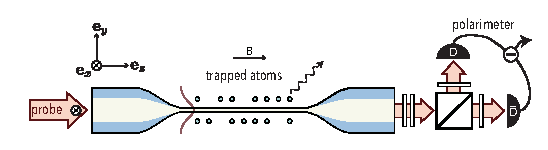
\includegraphics[width=.98\textwidth]{fig/Fig_NanofiberSchematicFaraday}
    \label{fig:Fig_NanofiberSchematicFaraday}
    \end{minipage} }\\
  %\end{subfloat}\\%   
  \subfloat[b][]{
  \begin{minipage}[bt]{.5\textwidth}
      \centering
      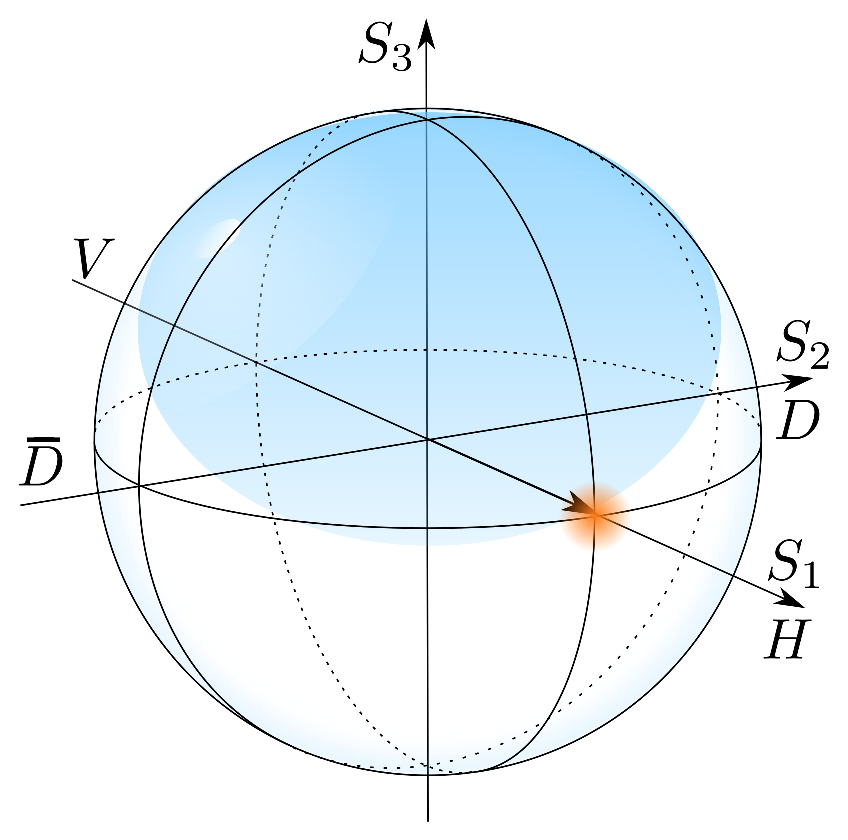
\includegraphics[width=.45\textwidth]{fig/poincaresphere_initialS1_crystal}
      \label{fig:poincaresphere_initialS1_crystal}
   \hfill
        \centering
        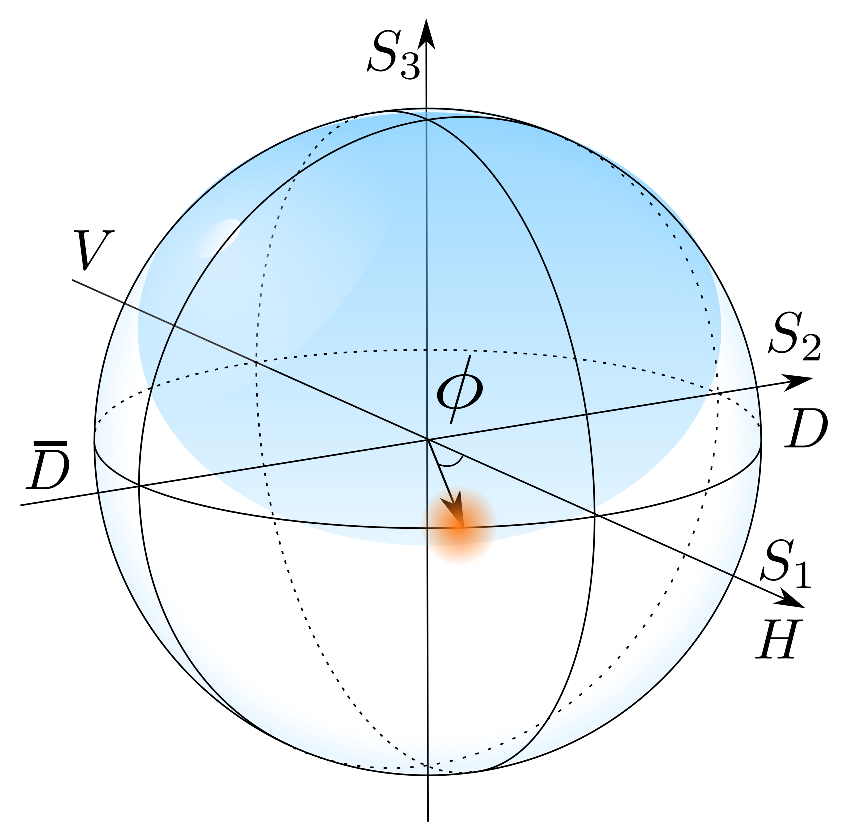
\includegraphics[width=.45\textwidth]{fig/poincaresphere_initialS1_Faradayrot_crystal}
        \label{fig:poincaresphere_initialS1_Faradayrot_crystal}
   \vfill
    \centering
    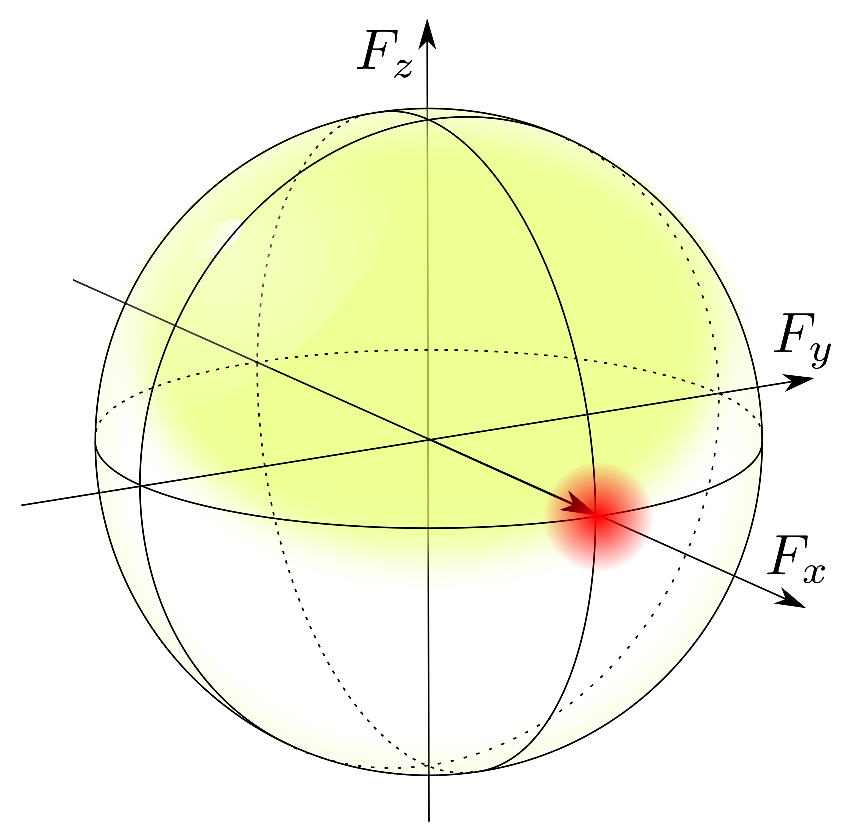
\includegraphics[width=.45\textwidth]{fig/blochsphere_initialxFxyz_crystal_orange}
    \label{fig:blochsphere_initialxFxyz_crystal_orange}
   \hfill
      \centering
      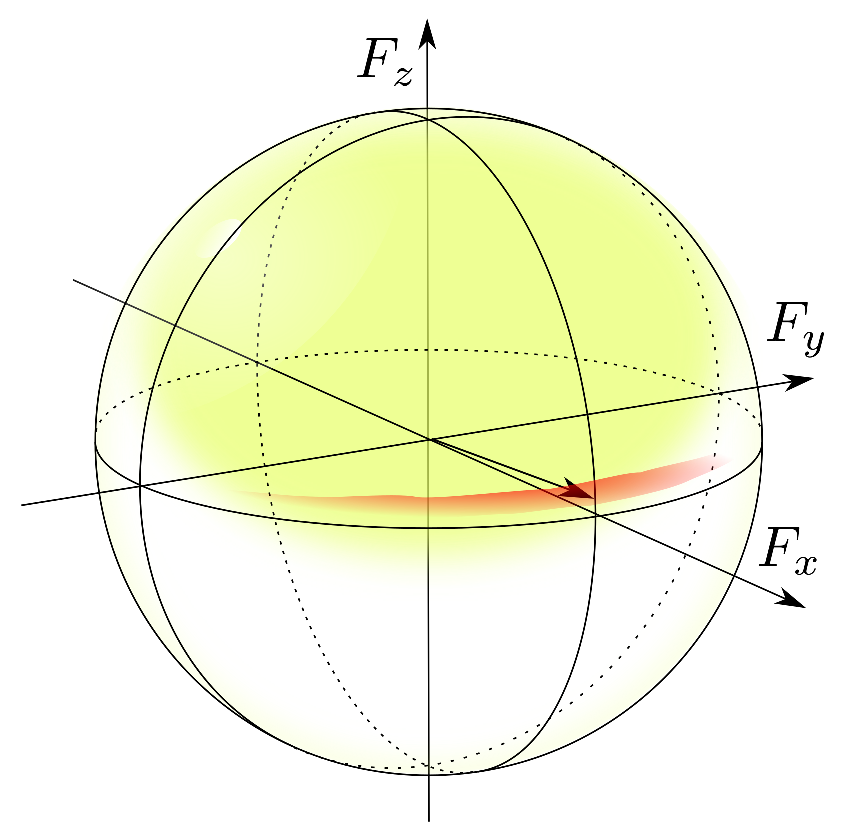
\includegraphics[width=.45\textwidth]{fig/blochsphere_initialxFxyz_squeezed_crystal_orange}
      \label{fig:blochsphere_initialxFxyz_squeezed_crystal_orange}
  \end{minipage}}\hfill
  %\end{subfloat}% 
  \subfloat[b][]{
  \begin{minipage}[bt]{.45\textwidth}
        \centering
        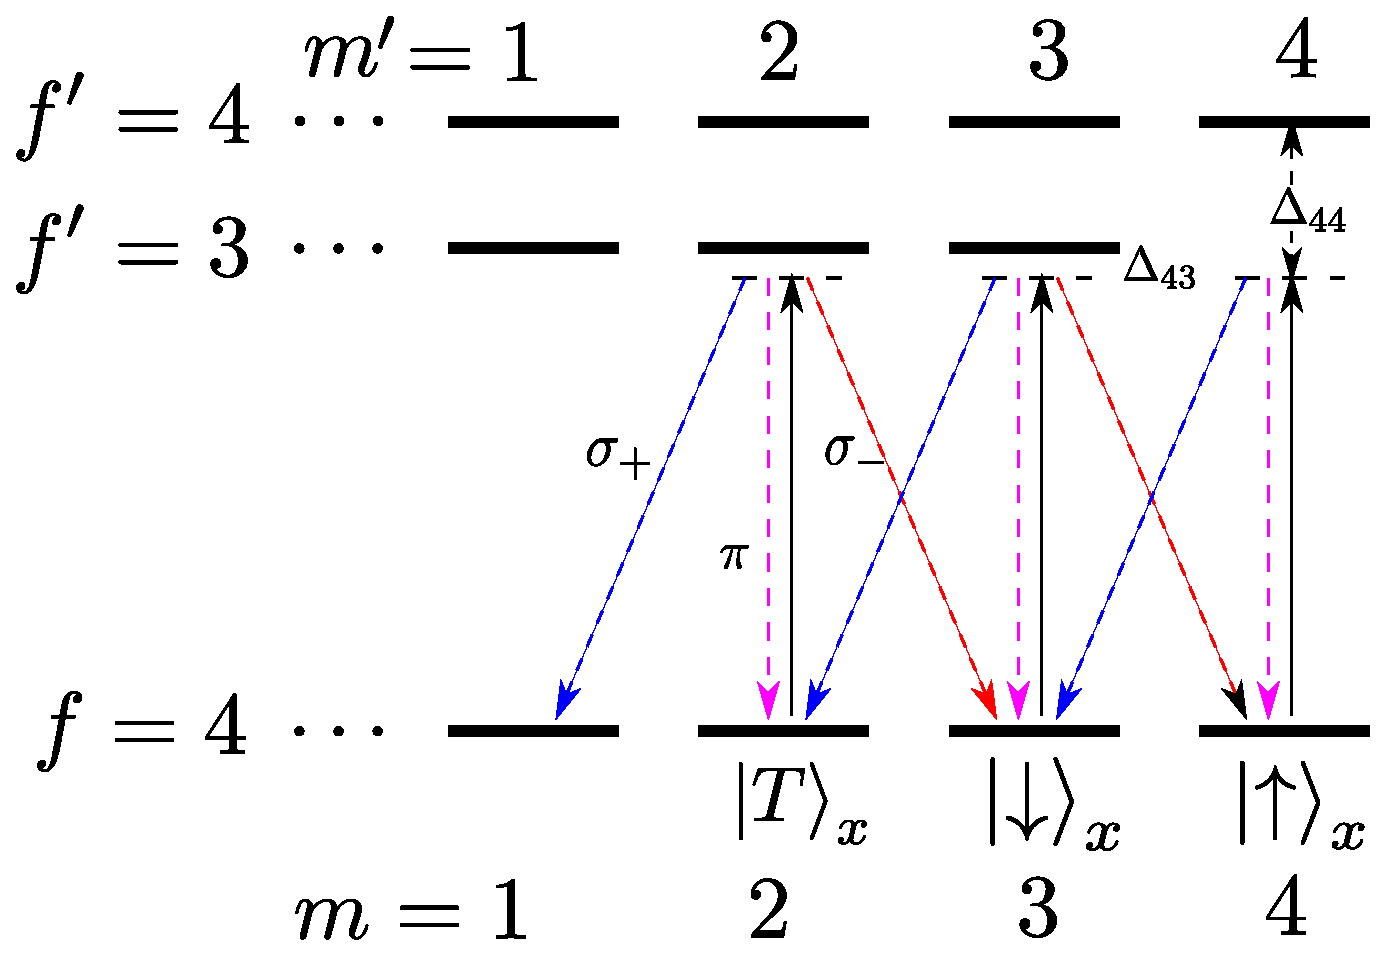
\includegraphics[width=.98\textwidth]{fig/stretchedstatestransitions_dashline}
        \label{fig:stretchedstatestransitions}
    \end{minipage}}
    %\end{subfloat}
  \caption{Illustrated are the schematic polarization spectroscopy setup for the QND measurement and spin squeezing generation based on the Faraday effect (a), evolution of the light (top row of (b)) and collective spin states (bottom row of (b)) before and after the measurement, and the internal atomic state transitions in the optical pumping process (c). Diagram (a) is adapted from Ref.~\cite{Qi2016}.}\label{fig:spinsqueezingschematic}
\end{figure}


In the following discussions, we will define the spin squeezing operator $ \hat{F}_\perp=\hat{F}_z=\sum_i\hat{f}_z^{(i)} $. 
We define the fiducial state of an atom as the \textit{up state}, or $ \ket{\uparrow} $. 
Applying $ \hat{f}_z $ on the fiducial state will yield the coupled state or $ \ket{\downarrow} $.
That is, $ \hat{f}_z^{(i)}\ket{\uparrow}^{(i)}\rightarrow \ket{\downarrow}^{(i)} $ for each atom.

To study the spin dynamics, we formally define a stochastic master equation of the atomic ensemble by
\begin{align}\label{eq:totaldrhodt}
\mathrm{d}\hat{\rho}=\left.\mathrm{d}\hat{\rho}\right|_{op} + \left.\mathrm{d}\hat{\rho}\right|_{QND}.
\end{align}
It includes two collective spin dynamic processes. 
The first process is the optical pumping dynamics on each individual atom $i$ positioned at $\br'$ which yields the $\mathrm{d}\hat{\rho}|_{op}=\sum_i^{N_A} \left.\mathrm{d}\hat{\rho}^{(i)}\right|_{op} $ term given by
\begin{align}
&\quad\left.\mathrm{d}\hat{\rho}^{(i)}\right|_{op} =\gamma_s\mathcal{D}^{(i)}\mathrm{d}t\\
&= -\frac{i\gamma_s}{\hbar} \left\{\hat{h}_{\rm eff},\hat{\rho}^{i} \right\}\mathrm{d}t + \gamma_s\sum_q \hat{W}_q(\br')\hat{\rho}^{i}\hat{W}_q^\dagger(\br')\mathrm{d}t,
\end{align}
where the characteristic photon scattering rate $ \gamma_s\equiv \frac{\Gamma_0\Omega^2}{4\Delta_F}=\frac{\sigma_0}{A_{in}}\frac{\Gamma_0^2}{4\Delta_F^2}\dot{N}_L $ with the effective input mode area $ A_{in}=1/n_g|u_{\mathrm{in}}(\br'\!_\perp)|^2 $ and the effective detuning $ \Delta_F $ defined by $ \frac{1}{\Delta_F}=\sum_{f'}\frac{C_{f'ff'}^{(1)}}{\Delta_{ff'}} $ and $ \Delta_{ff'}=\omega-\omega_{ff'} $, where $ \omega_{ff'} $ is the resonance angular frequency between the ground hyperfine structure level $ f $ and the excited hyperfine structure level $ f' $, and $ C_{j'ff'}^{(K)} $ are the coefficients for irreducible rank-$K$ components defined in \cite{Deutsch2010a}.
$\gamma_s$ characterizes the rate of decoherence dynamics and is proportional to the local photon flux of the probe light, $ \dot{N}_L $.

The second term on the right-hand side of Eq.\eqref{eq:totaldrhodt} gives rise to the collective spin dynamics due to QND measurement,
\begin{align}
\left.\mathrm{d}\hat{\rho}\right|_{QND} &= \sqrt{\frac{\kappa}{4}}\mathcal{H}\left[\hat{\rho} \right]\mathrm{d}W + \frac{\kappa}{4}\mathcal{L}\left[ \hat{\rho}\right]\mathrm{d}t.
\end{align}
Above, we have defined the measurement strength $\kappa \equiv |\chi|^2\dot{N}_L\equiv \frac{\sigma_0A_{in}}{A_{int}^2}\gamma_s $ determining the rate of the spin squeezing in absence of decoherent processes, where $\dot{N}_L$ is the photon number flux, $\chi$ is the light-atom coupling strength and $A_{int}$ is the effective interaction mode area which can be specified for a particular QND measurement protocol. We have also assumed the measurement backation is a stochastic Weiner process where $\mathrm{d}W$ is the increment satisfying $\mathrm{d}W^2 = \mathrm{d}t$. The conditional dynamics responding to the measurement evolve under the superoperator
\begin{align}
\mathcal{H}\left[ \hat{\rho}\right] &= \hat{F}_\perp\hat{\rho} + \hat{\rho}\hat{F}_\perp -2\expect{\hat{F}_\perp}\hat{\rho}
\end{align}
and the collective Lindblad map due to the direct photon scattering of the guided modes from the atoms
\begin{align}
\mathcal{L}\left[ \hat{\rho} \right] &= \hat{F}_\perp\hat{\rho}\hat{F}_\perp-\frac{1}{2}\left(\hat{\rho}\hat{F}_\perp^2+\hat{F}_\perp^2\hat{\rho} \right)=\frac{1}{2}\left[\hat{F}_\perp,\left[\hat{\rho},\hat{F}_\perp \right] \right].
\end{align}

As shown in the equations above, the spin squeezing dynamics is a competition between the coherent squeezing process and all decoherent processes which are characterized by $\kappa$ and $\gamma_s$, respectively. 
If we define an effective cooperativity or optical depth (OD) per atom quantity for the spin squeezing dynamics by
\begin{align}
\frac{\mathrm{OD}_{\rm eff}}{N_A} \equiv \frac{\kappa}{\gamma_s}=\frac{\sigma_0A_{in}}{A_F^2},
\end{align}
the peaking spin squeezing dynamics can then be characterized by $\frac{\mathrm{OD}_{\rm eff}}{N_A}$, and the geometry of the spin squeezing protocol can then be roughly designed with the goal to maximize $\frac{\mathrm{OD}_{\rm eff}}{N_A}$ by minimizing $A_{in}$ and maximizing $A_{int}$.  

We can bring in the spin coherence operator $\hat{\sigma}_{ba}=\ket{b}\bra{a}$ to represent the matrix element of any atomic angular momentum operator $ \hat{f}_m $ ($ m=x,y,z $) of a single atom, and hence the spin squeezing dynamics can be characterized by the expectation value of single-body spin coherence operators $\expect{\hat{\sigma}_{ba}}$ and the symmetric two-body covariances $\expect{\Delta \sigma_{ba}^{(1)}\Delta\sigma_{dc}^{(2)} }_s$. 
%the symmetric three-body correlations $\expect{\Delta \sigma^{(1)}_{b_1a_1}\Delta \sigma^{(2)}_{b_2a_2}\Delta \sigma^{(3)}_{b_3a_3} }_s$ and so on. 
%As higher-order correlations becomes negligible, one can cut off the correlation terms at a certain order.
If one can truncate the spin dynamics up to the two-body correlations, we only need the following two sets of stochastic differential equations:
\begin{subequations}
\begin{align}
d\expect{\hat{\sigma}_{ba}} &=\left. d{\expect{\hat{\sigma}_{ba}}}\right|_{op} + \left. d{\expect{\hat{\sigma}_{ba}}}\right|_{\mathcal{H}}+\left. d{\expect{\hat{\sigma}_{ba}}}\right|_{\mathcal{L}} \\
d\expect{\Delta \sigma_{ba}^{(1)}\Delta \sigma_{dc}^{(2)}}_s &= \left. d{\expect{\Delta \sigma_{ba}^{(1)}\Delta \sigma_{dc}^{(2)}}_s}\right|_{op} + \left. d{\expect{\Delta \sigma_{ba}^{(1)}\Delta \sigma_{dc}^{(2)}}_s}\right|_{\mathcal{H}} + \left. d{\expect{\Delta \sigma_{ba}^{(1)}\Delta \sigma_{dc}^{(2)}}_s}\right|_{\mathcal{L}}.
\end{align}
\end{subequations}

In details, the optical dynamics part can be given by
\begin{align}
\left. \dt{\expect{\hat{\sigma}_{ba}}}\right|_{op} &= \gamma_s\expect{\mathcal{D}^\dagger \left[ \hat{\sigma}_{ba}\right]}\\
&= \gamma_s\sum_{d,c}\tr\left(\mathcal{D}^\dagger \left[ \hat{\sigma}_{ba}\right]\hat{\sigma}_{dc} \right)\expect{\hat{\sigma}_{dc} }\\
\left. \dt{\expect{\Delta \sigma_{ba}^{(1)}\Delta \sigma_{dc}^{(2)}}_s}\right|_{op} &=\gamma_s\expect{\Delta\mathcal{D}^\dagger[\hat{\sigma}_{ba}^{(1)}]\Delta\sigma_{dc}^{(2)} }_s + \gamma_s\expect{\Delta\sigma_{ba}^{(1)}\Delta\mathcal{D}^\dagger[\hat{\sigma}_{dc}^{(2)}] }_s\\
&= \gamma_s\sum_{m,n}\tr\left(\mathcal{D}^\dagger[\hat{\sigma}_{ba}]\hat{\sigma}_{mn} \right)\expect{\Delta \sigma_{mn}^{(1)}\Delta \sigma_{dc}^{(2)} }_s + \gamma_s\sum_{m,n}\tr\left(\mathcal{D}^\dagger[\hat{\sigma}_{dc}]\hat{\sigma}_{mn} \right) \expect{\Delta \sigma_{ba}^{(1)}\Delta \sigma_{mn}^{(2)} }_s.
\end{align} 
Similarly, we will need the one- and two-body correlations due to the $ \mathcal{H} $ and $ \mathcal{L} $ superoperators given by the following.
\begin{subequations}
\begin{align}
\left.d\expect{\hat{\sigma}_{ba}}\right|_\mathcal{H} &=\sqrt{\frac{\kappa}{4}}\expect{\mathcal{H}^\dagger\left[\hat{\sigma}_{ba} \right]}dW \\
\left.d\expect{\hat{\sigma}_{ba}}\right|_\mathcal{L} &= \frac{\kappa}{4}\expect{\mathcal{L}^\dagger\left[\hat{\sigma}_{ba} \right]}dt
\end{align}
\end{subequations}
In principle, the two-body covariance terms can be coupled to high-order many-body terms. 
In our case, we assume the state of the ensemble can be well captured in the symmetric Gaussian state limit, and hence the two-body covariance equations due to the collective measurement can be given by
\begin{subequations}
\begin{align}
\left.d\expect{\Delta \sigma_{ba}^{(1)} \Delta \sigma_{dc}^{(2)}}_s \right|_\mathcal{H} &= -\kappa\expect{\Delta\sigma_{ba}^{(1)}\Delta F_\perp }_s \expect{\Delta F_\perp \Delta \sigma_{dc}^{(2)} }_s dt \\
\left.d\expect{\Delta \sigma_{ba}^{(1)} \Delta \sigma_{dc}^{(2)}}_s\right|_\mathcal{L} &= 0.
\end{align}
\end{subequations}

\subsection{A spin squeezing protocol using Faraday interaction with spin coherent states}

\begin{figure}[htb]
\centering
  \begin{subfloat}[h][Field components of the $H$-modes]{
    \centering
    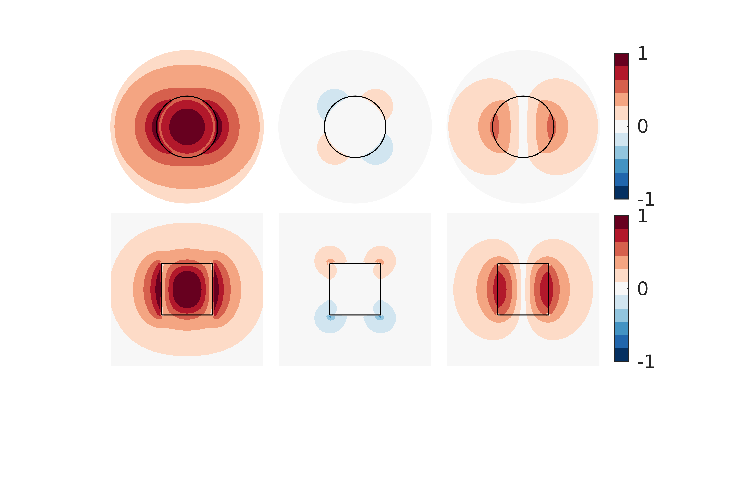
\includegraphics[width=.48\textwidth]{fig/nanofiberswg_Hmode_E_xy}
    \label{fig:nanofiber_Hmode_E_xy} }
  \end{subfloat}\\%   
  \begin{subfloat}[h][Intensity and field vector along $ y $-axis]{
    \centering
    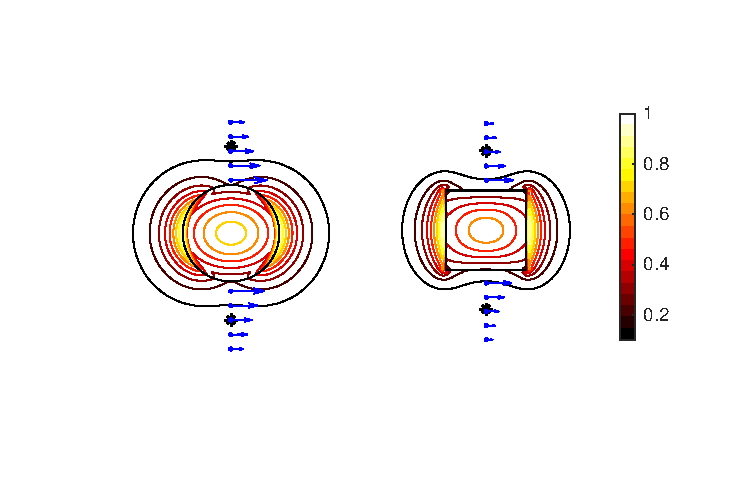
\includegraphics[width=.48\textwidth]{fig/nanofiberswg_Hmode_Ints_xy}
    \label{fig:nanofiber_Hmode_Ints_xy}}
  \end{subfloat}%  
  \caption{$H$-mode components and intensity distribution in the $ xy $-plane for the optical nanofiber and SWG. Shown on the first row, from left to right, are the real part of $ E_x(\br\!_\perp) $, the real part of $ E_z(\br\!_\perp) $ and the imaginary part of $ E_z(\br\!_\perp) $ for the nanofiber. White lines outline the waveguide boundary. The scale is normalized to the maximum value of all field components shown on the subplots. Plots on the second row are the same components as the first row but for the SWG. All the other parts of the electric field components of the $ H $- or TE$_{01}$-mode not shown in these plots for both waveguide geometries are zero everywhere. On the third row, we plot the normalized intensity distribution on the transverse plane for both geometries. The arrows indicates the local field's direction and amplitude (relative length) along the vertical waveguide axis, which only have an $ x $-component. The $ V $-mode is the $ H $-mode rotated by $ 90^\circ $ around the waveguide axis. }\label{fig:nanofiberswg_E_ints}
\end{figure}

\comment{To be done: Double check all equations in this section.}

Following the process demonstrated in our previous work~\cite{Qi2016}, the light-atom interaction Hamiltonian with one atom can be written as
\begin{align}
\hat{h}_\eff &= -\hat{\mathbf{E}}^{(-)}(\br')\cdot\hat{\tensor{\mathbf{\alpha}}}\cdot\hat{\mathbf{E}}^{(+)}(\br')\nn\\
&= -\frac{2\pi\hbar\omega}{v_g}\left[\mathbf{u}_H^*\cdot\hat{\tensor{\mathbf{\alpha}}}\cdot \mathbf{u}_H\hat{a}_H^\dagger\hat{a}_H\right.
+ \mathbf{u}_H^*\cdot\hat{\tensor{\mathbf{\alpha}}}\cdot \mathbf{u}_V\hat{a}_H^\dagger\hat{a}_V\nn\\
&\quad\quad + \mathbf{u}_V^*\cdot\hat{\tensor{\mathbf{\alpha}}}\cdot \mathbf{u}_H\hat{a}_V^\dagger\hat{a}_H 
\left. + \mathbf{u}_V^*\cdot\hat{\tensor{\mathbf{\alpha}}}\cdot \mathbf{u}_V\hat{a}_V^\dagger\hat{a}_V\right]\\
&= \hbar\left[(\hat{\chi}_{HH}+\hat{\chi}_{VV})\hat{S}_0 + (\hat{\chi}_{HH}-\hat{\chi}_{VV})\hat{S}_1 + (\hat{\chi}_{HV}+\hat{\chi}_{VH})\hat{S}_2 + i(\hat{\chi}_{HV}-\hat{\chi}_{VH})\hat{S}_3 \right]\\
%\hbar \left[\left(\chi_{RR\uparrow} + \chi_{RR\downarrow} +\chi_{LL\uparrow}+\chi_{LL\downarrow} \right)\hat{F}_0\hat{S}_0 \right.\nonumber\\
%&\quad+\left(\chi_{RR\uparrow} + \chi_{RR\downarrow} -\chi_{LL\uparrow}-\chi_{LL\downarrow} \right)\hat{F}_0\hat{S}_3\nonumber\\
%&\quad+\left(\chi_{RR\uparrow} + \chi_{LL\uparrow} -\chi_{RR\downarrow}-\chi_{LL\downarrow} \right)\hat{F}_3\hat{S}_0\nonumber\\
%&\quad+\left(\chi_{RR\uparrow} - \chi_{RR\downarrow} +\chi_{LL\downarrow}-\chi_{LL\uparrow} \right)\hat{F}_3\hat{S}_3\nonumber\\
%&\quad+i\left(\chi_{LR\uparrow} - \chi_{RL\uparrow} +\chi_{RL\downarrow}-\chi_{RL\downarrow} \right)\hat{F}_0\hat{S}_1\nonumber\\
%&\quad+\left(\chi_{RL\uparrow} + \chi_{LR\uparrow} +\chi_{RL\downarrow}+\chi_{LR\downarrow} \right)\hat{F}_0\hat{S}_2\nonumber\\
%&\quad+i\left(\chi_{LR\uparrow} - \chi_{RL\uparrow} +\chi_{RL\downarrow}-\chi_{LR\downarrow} \right)\hat{F}_3\hat{S}_1\nonumber\\
%&\quad+\left.\left(\chi_{LR\uparrow} + \chi_{RL\uparrow} -\chi_{LR\downarrow}-\chi_{RL\downarrow} \right)\hat{F}_3\hat{S}_2 \right]\\
&=\hbar\sum_{i=0}^3 \hat{\chi}_{i}\hat{S}_i\\
&=\hbar\sum_{i,j=0} \chi_{ij}\hat{f}_i\hat{S}_j,
\end{align}
where $ \hat{S}_i $ are the Stokes vector operators of the light indicating its polarization, and the mode-atom coupling operator
\begin{align}
\hat{\chi}_{pp'} 
&=-\frac{2\pi \omega}{v_g}\mathbf{u}_{p}^*(r'\!_\perp,\phi')\cdot \hat{\tensor{\alpha}}\cdot \mathbf{u}_{p'}(r'\!_\perp,\phi')\\
&= \sum_{f'} \frac{n_g\sigma_0}{4}\frac{\Gamma_{f'}}{\Delta_{ff'}+i\Gamma_{f'}/2}\cdot \left\{ C_{j'ff'}^{(0)}\mathbf{u}_p^*(r'\!_\perp)\cdot \mathbf{u}_{p'}(r'\!_\perp)\hat{\mathbbm{1}}\right.\nn\\
&\quad\quad +iC_{j'ff'}^{(1)}\left(\mathbf{u}_p^*(r'\!_\perp)\times\mathbf{u}_{p'}(r'\!_\perp) \right)\cdot \hat{\mathbf{f}} \nonumber\\
&\quad\quad\left. + C_{j'ff'}^{(2)}\sum_{i,j}\left[u^*_{p,i}u_{p',j}(\frac{\hat{f}_i\hat{f}_j+\hat{f}_j\hat{f}_i}{2}-\frac{\delta_{ij}}{3}\hat{\mathbf{f}}\cdot\hat{\mathbf{f}}) \right]\right\}
%&\left.+C_{jj'ff'}^{(2)}\left[\mathbf{u}_p^*(r'\!_\perp)\cdot \mathbf{u}_{p'}(r'\!_\perp)\left(\frac{f(f+1)}{6}-\frac{m^2}{2} \right)+\mathbf{u}_p^*(r'\!_\perp)\cdot (\hat{e}^*_{\tilde{z}}\hat{e}_{\tilde{z}})\cdot \mathbf{u}_{p'}(r'\!_\perp)\left(\frac{3m^2}{2}-\frac{f(f+1)}{2} \right) \right] \right\}
\label{eq:chippp}
\end{align}
with the horizontally(H)- and vertically(V)-linearly polarized guided modes, $ \mathbf{u}_p(r'\!_\perp) $, at the atom position $ \br'=(r'\!_\perp,\phi',z') $. 
$ \chi_{ij}=\tr[\hat{f}_i\hat{\chi}_j]/(2f+1) $ is the coupling strength between spin operator $ \hat{f}_i $ and Stokes operator $ \hat{S}_j $. 
For example, $ \chi_{33} $ is the coupling strength between $ \hat{f}_z $ and $ \hat{S}_3 $.
The fundamental guided modes of an optical nanofiber has been defined in the appendix of our previous paper~\cite{Qi2016}. 
In general, for a cylindrical waveguide, the H- and V-modes are the guided modes adiabatically transferred from a corresponding linearly polarized input light from one end of the waveguide, where H- and V-directions are orthogonal to each other in the transverse plane.
The coupling operator or Eq.\eqref{eq:chippp} includes three terms corresponding to scalar, vector and tensor interactions between atoms and the probe light which are proportional to $ C_{j'ff'}^{(K)} $ with $ K=0,\,1,\,2 $, respectively.

Faraday interaction is the interaction when the helicity of the input and output of the light signal is preserved. 
In the context of QND measurement, a Faraday interaction based protocol is the protocol when the phase change of the output light on the equator of the \Poincare sphere with a linear polarization input is used to calibrate the spin state after the atom-light interaction.
This phase change of light polarization corresponds to a rotation about $ \mathbf{S}_3 $ axis on the \Poincare sphere. 
From Eq.\eqref{eq:chippp}, the coupling atomic term is proportional to 
\begin{align}
\hat{\chi}_{i3} &= \hat{\chi}_{HV}-\hat{\chi}_{VH}=\hat{\chi}_{RR}-\hat{\chi}_{LL},
\end{align}
where the last step is derived in appendix~\ref{Appendix:LRbases}. These relationships indicate the Faraday effect is generated by the intensity or photon number difference between the right- and left-polarized modes or by the phase difference between two linearly polarized modes due to the polarizability of the atoms.
One can prove that the strength of the Faraday interaction is dominated by the vector interaction term in Eq.\eqref{eq:chippp}.
This implies that, to maximize the Faraday interaction, it is optimal to choose a quantization axis along the direction of $ \mathbf{v}_F=\mathbf{u}_H^*(\br'\!_\perp)\!\times\!\mathbf{u}_{V}(\br'\!_\perp)\!-\!\mathbf{u}_V^*(\br'\!_\perp)\!\times\!\mathbf{u}_{H}(\br'\!_\perp)$ given the atoms are placed at $ \br'\!_\perp $ position in the transverse plane of the waveguide. 
In reality, this product of modes may be elliptical with at least one direction component is imaginary while others are real.
If this happens, since the quantization axis is the direction in which a magnetic field is pointing to in 3D real space, the optimal choice of quantization axis should be the direction corresponding to the largest component of the $ \mathbf{v}_F $ vector. 
For a cylindrical waveguide, this doesn't seem to happen.
Take the example of a nanofiber, at an arbitrary position $ \br'\!_\perp=(r'\!_\perp,\phi') $ of atoms in the transverse plane,
\begin{align}
\mathbf{u}_H^*(r'\!_\perp,\phi')\times \mathbf{u}_V(r'\!_\perp,\phi') &= 2u_{r\!_\perp} u_\phi\mathbf{e}_z - 2iu_zu_{r\!_\perp}\sin2\phi \mathbf{e}_\phi + 2iu_\phi u_z\cos2\phi \mathbf{e}_{r\!_\perp} \\
\mathbf{u}_V^*(r'\!_\perp,\phi')\times \mathbf{u}_H(r'\!_\perp,\phi') &= -2u_{r\!_\perp} u_\phi\mathbf{e}_z - 2iu_zu_{r\!_\perp}\sin2\phi \mathbf{e}_\phi + 2iu_\phi u_z\cos2\phi \mathbf{e}_{r\!_\perp},
\end{align}
and therefore,
\begin{align}\label{eq:Faradayaxis}
\mathbf{v}_F=\mathbf{u}_H^*(\br'\!_\perp)\!\times\!\mathbf{u}_{V}(\br'\!_\perp)\!-\!\mathbf{u}_V^*(\br'\!_\perp)\!\times\!\mathbf{u}_{H}(\br'\!_\perp) = 4u_{r\!_\perp} u_\phi\mathbf{e}_z,
\end{align}
where $ u_{r\!_\perp}=u_{r\!_\perp}(r'\!_\perp) $, $ u_\phi=u_\phi(r'\!_\perp) $ and $ u_z=u_z(r'\!_\perp) $ are the right-circularly polarized mode components independent of longitudinal and azimuthal positions defined in the appendix A of Ref~\cite{Qi2016} or the corresponding appendix in this dissertation.
Based on this result, choosing $ z $-direction as the quantization axis is optimal for the QND measurement and spin squeezing protocol for atoms trapped near an optical nanofiber.

This conclusion can be generalized to cylindrical waveguides at large, which have a smooth or slow change of index of refraction along the light propagation direction in the wavelength scale while the cross-section of the waveguides can be arbitrary.
From the perspective of transformation optics~\cite{Leonhardt2006Optical,Kundtz2011Electromagnetic}, we can consider a set of $H$- and $V$-modes for the new waveguide are generated by adiabatically transforming the orthogonal set of modes from a cylindrical nanofiber to the target cross-section shape of the waveguide.
Since the transformation is approximately limited to the $xy$-plane of the coordinate system transformation determined by a Jacobian matrix, Eq.\eqref{eq:Faradayaxis} will preserve the form in the new waveguide coordinate system where only $ z $-component is non-zero and should be chosen as the optimal choice of the quantization axis.

With the quantization axis chosen along $ \mathbf{e}_{\tilde{z}}=\mathbf{e}_z $, one can define the effective QND measurement Hamiltonian for an atomic ensemble by
\begin{align}
\hat{H}_F &= \hbar \chi_{33}\hat{F}_z \hat{S}_3,
\end{align}
where $ \chi_{33} $ is the measurement strength characterizing the entanglement between the collective spin state of $ \hat{F}_z $ and the probe's polarization state of $ \hat{S}_3 $.
Now that $ \hat{F}_\perp=\hat{F}_z $ is the squeezing operator. 
Let us consider an ensemble of $ ^{133} $Cs atoms initially prepared as a spin coherent state (SCS) with every atom in the stretch state of the $ 6S_{1/2}$ $f=4 $ ground manifold in the $ x $-basis, where the quantization $ x $-direction is along the diagonal or $ \phi=\pi/4 $ direction in the $ H $-$ V $ Cartesian coordinate system sitting on the fiber axis.
One can show that a stretch state can generate the maximum coupling between atoms and light when all atoms are prepared in a SCS.
We call this initial state of one atom as the fiducial state or $ \ket{\phi_0}=\ket{\uparrow}_x = \ket{6S_{1/2},f=4,m_x=4} $ and the collective SCS can be written as $ \ket{\Psi_0}=\ket{\uparrow}_x^{\otimes N_A} $.
We define the coupled state by applying the individual squeezing operator $ \hat{f}_z$ on the fiducial state $\ket{\uparrow}_x $.
In our case, the coupled state can be defined as $ \ket{\downarrow}_x=\ket{6S_{1/2},f=4,m_x=3} $.
Similarly, to include the transfer of coherence in the squeezing process, we define the transfer state as $ \ket{T}_x=\ket{6S_{1/2},f=4,m_x=2} $ resulted from applying $ \hat{f}_z$ on the coupled state. 
For simplicity, we remove all the subscript $ x $ of quantum states and assume we always work in the $ x $-basis if no explicit notations for the Faraday interaction protocol. 

We consider the far-detuning regime, where we may be able to set the decay rates of the excited levels $ \Gamma_{f'}= \Gamma_0$ as constant for all $ f' $ in the same fine structure manifold, where we consider $ \Gamma_0 $ as the averaged modified decay rates from the excite fine structure level to the ground level when atoms are in a completely mixed state for simplicity.
We also ignore the tensor coupling strength related to $ C_{jj'ff'}^{(2)} $ terms in Eq.\eqref{eq:chippp} as the tensor interaction strength ($ \sim 1/\Delta^2 $) is relatively small compared to the vector interaction strength ($ \sim 1/\Delta $)~\cite{Deutsch2010a}. 
For a nanofiber geometry, the Faraday interaction coupling strength is independent of the azimuthal position of the atoms and can be simplified as
\begin{align}
\chi_{33} &= -\sum_{f'}n_g\sigma_0\frac{\Gamma_0}{\Delta_{ff'}+i\Gamma_0/2}C_{jj'ff'}^{(1)}u_{r\!_\perp}(r'\!_\perp)u_\phi(r'\!_\perp)\\
&=\frac{\sigma_0}{A_F}\frac{\Gamma_0}{\Delta_F},
\end{align}
where the effective Faraday interaction mode area $ A_F=1/2n_g|u_{r\!_\perp}(r'\!_\perp)u_\phi(r\!_\perp)| $, and the effective detuning $ \Delta_F=\sum_{f'}\frac{-C_{j'ff'}^{(1)}}{\Delta_{ff'}} $.
The measurement strength is now defined as
\begin{align}
\kappa\equiv|\chi_{33}|^2\dot{N}_L=\frac{\sigma_0A_{in}}{A_F^2}\gamma_s,
\end{align}
where the characteristic photon scattering rate $ \gamma_s\equiv \frac{\Gamma_0\Omega^2}{4\Delta_F}=\frac{\sigma_0}{A_{in}}\frac{\Gamma_0^2}{4\Delta_F^2}\dot{N}_L $ and the effective mode area $ A_{in}=1/n_g|u_{\mathrm{in}}(\br'\!_\perp)|^2 $.
Now we can define the OD per atom for the Faraday interaction using SCS by
\begin{align}
\frac{\mathrm{OD}}{N_A} \equiv \frac{\kappa}{\gamma_s}=\frac{\sigma_0A_{in}}{A_F^2}.
\end{align}

Since the Faraday measurement strength doesn't depend on the azimuthal direction of the atom position, ideally, to implement an optimal Faraday interaction geometry, it is preferable to place atoms along some azimuthal direction with the minimum impact from birefringence effects as well as the decoherence due to the presence of the nanofiber. 

Firstly, in the far-detuning regime, since the birefringence effect is dominated by the scalar coupling which is proportional to the intensity difference between the $H$ ($x$)- and $V$ ($ y $)-mode components at the atom positions, both diagonal and anti-diagonal directions in the transverse plane yields a minimum birefringence effect where the intensity of the $ H $- and $ V $-mode components are equal, based on the symmetry of the fiber and given a diagonally polarized $ D $-mode input.
That is the optimal position of atoms with vanished birefringence effect due to the intensity difference of the local $ H $- and $ V $-modes could be along the $ \phi'=n\pi/4 $ ($ n=1,3,5,7 $) radial directions. 
Secondly, to minimize the decoherence damages to spin squeezing, the optimal position of the atom should be chosen so that $ A_{\mathrm{in}} $ reaches the minimum value, which yields $ \phi'=3\pi/4 $ or $ 7\pi/4 $ where $ A_{\mathrm{in}}=1/2n_g|u_\phi(r'\!_\perp)|^2 $.
Combining these two factors, we find the optimal choice of atoms' azimuthal positions are along the anti-diagonal direction, that is $\phi'=3\pi/4 $ or $ 7\pi/4 $.

The number of equations needed to include different subspace...

\subsection{Decoherence and total angular momentum quantum number of atoms}

%=================== Simulations with waveguides =====================%
\section{Discussions} \label{Sec::Discussions}
\comment{Leave discussions on how does the internal structure of atoms and the total atomic quantum number affect the spin squeezing parameter for future works.}

% set package options
\captionsetup[subfloat]{position=top,singlelinecheck=off,labelfont={normalsize,sf}, %justification=raggedright,
  labelformat=simple,listofformat=subparens,aboveskip=0pt,parskip=0pt,farskip=5pt,
  captionskip=0pt}

% customize subfigure label to capitals
\renewcommand{\thesubfigure}{(\alph{subfigure})}

%\newlength\figureheight
%\newlength\figurewidth
\begin{figure}[htb]
\centering
%\pgfplotsset{yticklabel style={text width=3em,align=right}}
 \begin{minipage}[h]{0.2\linewidth}
 %\begin{tabular}{*{2}{b{0.2\textwidth-2\tabcolsep}}}
  \subfloat[h][$1/\AF$]{
    %\setlength\figureheight{0.3\textwidth}
    %\setlength\figurewidth{0.3\textwidth}
    % This file was created by matlab2tikz.
%
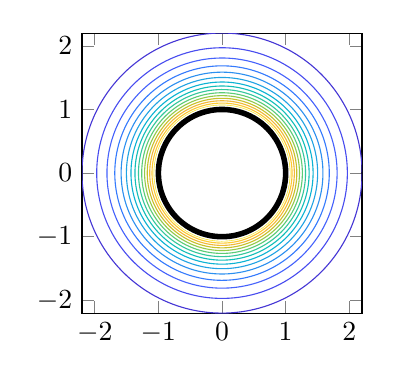
\begin{tikzpicture}

\begin{axis}[%
width=1.4in,
height=1.4in,
at={(0in,0in)},
scale only axis,
colormap={mymap}{[1pt] rgb(0pt)=(0.2422,0.1504,0.6603); rgb(1pt)=(0.25039,0.164995,0.707614); rgb(2pt)=(0.257771,0.181781,0.751138); rgb(3pt)=(0.264729,0.197757,0.795214); rgb(4pt)=(0.270648,0.214676,0.836371); rgb(5pt)=(0.275114,0.234238,0.870986); rgb(6pt)=(0.2783,0.255871,0.899071); rgb(7pt)=(0.280333,0.278233,0.9221); rgb(8pt)=(0.281338,0.300595,0.941376); rgb(9pt)=(0.281014,0.322757,0.957886); rgb(10pt)=(0.279467,0.344671,0.971676); rgb(11pt)=(0.275971,0.366681,0.982905); rgb(12pt)=(0.269914,0.3892,0.9906); rgb(13pt)=(0.260243,0.412329,0.995157); rgb(14pt)=(0.244033,0.435833,0.998833); rgb(15pt)=(0.220643,0.460257,0.997286); rgb(16pt)=(0.196333,0.484719,0.989152); rgb(17pt)=(0.183405,0.507371,0.979795); rgb(18pt)=(0.178643,0.528857,0.968157); rgb(19pt)=(0.176438,0.549905,0.952019); rgb(20pt)=(0.168743,0.570262,0.935871); rgb(21pt)=(0.154,0.5902,0.9218); rgb(22pt)=(0.146029,0.609119,0.907857); rgb(23pt)=(0.138024,0.627629,0.89729); rgb(24pt)=(0.124814,0.645929,0.888343); rgb(25pt)=(0.111252,0.6635,0.876314); rgb(26pt)=(0.0952095,0.679829,0.859781); rgb(27pt)=(0.0688714,0.694771,0.839357); rgb(28pt)=(0.0296667,0.708167,0.816333); rgb(29pt)=(0.00357143,0.720267,0.7917); rgb(30pt)=(0.00665714,0.731214,0.766014); rgb(31pt)=(0.0433286,0.741095,0.73941); rgb(32pt)=(0.0963952,0.75,0.712038); rgb(33pt)=(0.140771,0.7584,0.684157); rgb(34pt)=(0.1717,0.766962,0.655443); rgb(35pt)=(0.193767,0.775767,0.6251); rgb(36pt)=(0.216086,0.7843,0.5923); rgb(37pt)=(0.246957,0.791795,0.556743); rgb(38pt)=(0.290614,0.79729,0.518829); rgb(39pt)=(0.340643,0.8008,0.478857); rgb(40pt)=(0.3909,0.802871,0.435448); rgb(41pt)=(0.445629,0.802419,0.390919); rgb(42pt)=(0.5044,0.7993,0.348); rgb(43pt)=(0.561562,0.794233,0.304481); rgb(44pt)=(0.617395,0.787619,0.261238); rgb(45pt)=(0.671986,0.779271,0.2227); rgb(46pt)=(0.7242,0.769843,0.191029); rgb(47pt)=(0.773833,0.759805,0.16461); rgb(48pt)=(0.820314,0.749814,0.153529); rgb(49pt)=(0.863433,0.7406,0.159633); rgb(50pt)=(0.903543,0.733029,0.177414); rgb(51pt)=(0.939257,0.728786,0.209957); rgb(52pt)=(0.972757,0.729771,0.239443); rgb(53pt)=(0.995648,0.743371,0.237148); rgb(54pt)=(0.996986,0.765857,0.219943); rgb(55pt)=(0.995205,0.789252,0.202762); rgb(56pt)=(0.9892,0.813567,0.188533); rgb(57pt)=(0.978629,0.838629,0.176557); rgb(58pt)=(0.967648,0.8639,0.16429); rgb(59pt)=(0.96101,0.889019,0.153676); rgb(60pt)=(0.959671,0.913457,0.142257); rgb(61pt)=(0.962795,0.937338,0.12651); rgb(62pt)=(0.969114,0.960629,0.106362); rgb(63pt)=(0.9769,0.9839,0.0805)},
xmin=-2.2000,
xmax=2.2000,
ymin=-2.2000,
ymax=2.2000,
axis background/.style={fill=white}
]
\addplot[contour prepared, contour prepared format=matlab, contour/labels=false] table[row sep=crcr] {%
%
0.0556	180.0000\\
0.9932	-0.0000\\
0.9925	-0.0349\\
0.9907	-0.0697\\
0.9877	-0.1044\\
0.9834	-0.1390\\
0.9779	-0.1734\\
0.9712	-0.2076\\
0.9633	-0.2416\\
0.9543	-0.2752\\
0.9440	-0.3086\\
0.9326	-0.3415\\
0.9200	-0.3740\\
0.9063	-0.4061\\
0.8915	-0.4376\\
0.8756	-0.4687\\
0.8586	-0.4991\\
0.8406	-0.5289\\
0.8215	-0.5581\\
0.8014	-0.5866\\
0.7804	-0.6143\\
0.7583	-0.6414\\
0.7353	-0.6676\\
0.7115	-0.6930\\
0.6867	-0.7175\\
0.6611	-0.7412\\
0.6347	-0.7639\\
0.6075	-0.7857\\
0.5795	-0.8065\\
0.5509	-0.8264\\
0.5215	-0.8452\\
0.4915	-0.8630\\
0.4610	-0.8797\\
0.4298	-0.8953\\
0.3981	-0.9099\\
0.3659	-0.9233\\
0.3333	-0.9356\\
0.3003	-0.9467\\
0.2669	-0.9566\\
0.2331	-0.9654\\
0.1991	-0.9730\\
0.1648	-0.9794\\
0.1304	-0.9846\\
0.0957	-0.9885\\
0.0610	-0.9913\\
0.0261	-0.9928\\
-0.0087	-0.9931\\
-0.0436	-0.9922\\
-0.0784	-0.9901\\
-0.1131	-0.9867\\
-0.1476	-0.9821\\
-0.1820	-0.9763\\
-0.2161	-0.9694\\
-0.2500	-0.9612\\
-0.2836	-0.9518\\
-0.3168	-0.9413\\
-0.3497	-0.9296\\
-0.3821	-0.9167\\
-0.4140	-0.9028\\
-0.4454	-0.8877\\
-0.4763	-0.8715\\
-0.5066	-0.8542\\
-0.5363	-0.8359\\
-0.5653	-0.8166\\
-0.5936	-0.7963\\
-0.6212	-0.7749\\
-0.6480	-0.7527\\
-0.6740	-0.7294\\
-0.6992	-0.7053\\
-0.7235	-0.6804\\
-0.7469	-0.6546\\
-0.7694	-0.6279\\
-0.7910	-0.6006\\
-0.8116	-0.5724\\
-0.8312	-0.5436\\
-0.8498	-0.5141\\
-0.8673	-0.4839\\
-0.8837	-0.4532\\
-0.8991	-0.4219\\
-0.9133	-0.3901\\
-0.9265	-0.3578\\
-0.9385	-0.3251\\
-0.9493	-0.2919\\
-0.9589	-0.2585\\
-0.9674	-0.2246\\
-0.9747	-0.1905\\
-0.9808	-0.1562\\
-0.9857	-0.1217\\
-0.9893	-0.0870\\
-0.9918	-0.0523\\
-0.9930	-0.0174\\
-0.9930	0.0174\\
-0.9918	0.0523\\
-0.9893	0.0870\\
-0.9857	0.1217\\
-0.9808	0.1562\\
-0.9747	0.1905\\
-0.9674	0.2246\\
-0.9589	0.2585\\
-0.9493	0.2919\\
-0.9385	0.3251\\
-0.9265	0.3578\\
-0.9133	0.3901\\
-0.8991	0.4219\\
-0.8837	0.4532\\
-0.8673	0.4839\\
-0.8498	0.5141\\
-0.8312	0.5436\\
-0.8116	0.5724\\
-0.7910	0.6006\\
-0.7694	0.6279\\
-0.7469	0.6546\\
-0.7235	0.6804\\
-0.6992	0.7053\\
-0.6740	0.7294\\
-0.6480	0.7527\\
-0.6212	0.7749\\
-0.5936	0.7963\\
-0.5653	0.8166\\
-0.5363	0.8359\\
-0.5066	0.8542\\
-0.4763	0.8715\\
-0.4454	0.8877\\
-0.4140	0.9028\\
-0.3821	0.9167\\
-0.3497	0.9296\\
-0.3168	0.9413\\
-0.2836	0.9518\\
-0.2500	0.9612\\
-0.2161	0.9694\\
-0.1820	0.9763\\
-0.1476	0.9821\\
-0.1131	0.9867\\
-0.0784	0.9901\\
-0.0436	0.9922\\
-0.0087	0.9931\\
0.0261	0.9928\\
0.0610	0.9913\\
0.0957	0.9885\\
0.1304	0.9846\\
0.1648	0.9794\\
0.1991	0.9730\\
0.2331	0.9654\\
0.2669	0.9566\\
0.3003	0.9467\\
0.3333	0.9356\\
0.3659	0.9233\\
0.3981	0.9099\\
0.4298	0.8953\\
0.4610	0.8797\\
0.4915	0.8630\\
0.5215	0.8452\\
0.5509	0.8264\\
0.5795	0.8065\\
0.6075	0.7857\\
0.6347	0.7639\\
0.6611	0.7412\\
0.6867	0.7175\\
0.7115	0.6930\\
0.7353	0.6676\\
0.7583	0.6414\\
0.7804	0.6143\\
0.8014	0.5866\\
0.8215	0.5581\\
0.8406	0.5289\\
0.8586	0.4991\\
0.8756	0.4687\\
0.8915	0.4376\\
0.9063	0.4061\\
0.9200	0.3740\\
0.9326	0.3415\\
0.9440	0.3086\\
0.9543	0.2752\\
0.9633	0.2416\\
0.9712	0.2076\\
0.9779	0.1734\\
0.9834	0.1390\\
0.9877	0.1044\\
0.9907	0.0697\\
0.9925	0.0349\\
0.9932	0.0000\\
0.1111	180.0000\\
2.2008	0.0000\\
2.1995	0.0772\\
2.1954	0.1544\\
2.1887	0.2313\\
2.1792	0.3080\\
2.1670	0.3843\\
2.1522	0.4601\\
2.1347	0.5353\\
2.1146	0.6099\\
2.0919	0.6838\\
2.0667	0.7568\\
2.0388	0.8288\\
2.0085	0.8999\\
1.9757	0.9698\\
1.9404	1.0385\\
1.9028	1.1060\\
1.8628	1.1721\\
1.8205	1.2367\\
1.7760	1.2999\\
1.7293	1.3614\\
1.6804	1.4212\\
1.6295	1.4793\\
1.5766	1.5356\\
1.5217	1.5900\\
1.4650	1.6424\\
1.4064	1.6928\\
1.3462	1.7411\\
1.2842	1.7873\\
1.2207	1.8313\\
1.1557	1.8730\\
1.0893	1.9124\\
1.0215	1.9494\\
0.9524	1.9841\\
0.8822	2.0163\\
0.8109	2.0460\\
0.7386	2.0732\\
0.6654	2.0979\\
0.5914	2.1199\\
0.5166	2.1394\\
0.4412	2.1562\\
0.3653	2.1703\\
0.2889	2.1818\\
0.2121	2.1906\\
0.1351	2.1967\\
0.0579	2.2001\\
-0.0193	2.2008\\
-0.0965	2.1987\\
-0.1736	2.1940\\
-0.2505	2.1865\\
-0.3271	2.1764\\
-0.4033	2.1636\\
-0.4790	2.1481\\
-0.5541	2.1300\\
-0.6285	2.1092\\
-0.7021	2.0859\\
-0.7749	2.0599\\
-0.8467	2.0315\\
-0.9175	2.0005\\
-0.9871	1.9671\\
-1.0555	1.9312\\
-1.1227	1.8930\\
-1.1884	1.8524\\
-1.2527	1.8096\\
-1.3154	1.7645\\
-1.3765	1.7172\\
-1.4359	1.6679\\
-1.4936	1.6165\\
-1.5494	1.5630\\
-1.6033	1.5077\\
-1.6552	1.4505\\
-1.7051	1.3915\\
-1.7529	1.3308\\
-1.7985	1.2685\\
-1.8419	1.2046\\
-1.8831	1.1392\\
-1.9219	1.0724\\
-1.9583	1.0043\\
-1.9924	0.9350\\
-2.0240	0.8645\\
-2.0531	0.7929\\
-2.0796	0.7204\\
-2.1036	0.6470\\
-2.1250	0.5727\\
-2.1438	0.4978\\
-2.1600	0.4223\\
-2.1735	0.3462\\
-2.1843	0.2697\\
-2.1924	0.1929\\
-2.1978	0.1158\\
-2.2005	0.0386\\
-2.2005	-0.0386\\
-2.1978	-0.1158\\
-2.1924	-0.1929\\
-2.1843	-0.2697\\
-2.1735	-0.3462\\
-2.1600	-0.4223\\
-2.1438	-0.4978\\
-2.1250	-0.5727\\
-2.1036	-0.6470\\
-2.0796	-0.7204\\
-2.0531	-0.7929\\
-2.0240	-0.8645\\
-1.9924	-0.9350\\
-1.9583	-1.0043\\
-1.9219	-1.0724\\
-1.8831	-1.1392\\
-1.8419	-1.2046\\
-1.7985	-1.2685\\
-1.7529	-1.3308\\
-1.7051	-1.3915\\
-1.6552	-1.4505\\
-1.6033	-1.5077\\
-1.5494	-1.5630\\
-1.4936	-1.6165\\
-1.4359	-1.6679\\
-1.3765	-1.7172\\
-1.3154	-1.7645\\
-1.2527	-1.8096\\
-1.1884	-1.8524\\
-1.1227	-1.8930\\
-1.0555	-1.9312\\
-0.9871	-1.9671\\
-0.9175	-2.0005\\
-0.8467	-2.0315\\
-0.7749	-2.0599\\
-0.7021	-2.0859\\
-0.6285	-2.1092\\
-0.5541	-2.1300\\
-0.4790	-2.1481\\
-0.4033	-2.1636\\
-0.3271	-2.1764\\
-0.2505	-2.1865\\
-0.1736	-2.1940\\
-0.0965	-2.1987\\
-0.0193	-2.2008\\
0.0579	-2.2001\\
0.1351	-2.1967\\
0.2121	-2.1906\\
0.2889	-2.1818\\
0.3653	-2.1703\\
0.4412	-2.1562\\
0.5166	-2.1394\\
0.5914	-2.1199\\
0.6654	-2.0979\\
0.7386	-2.0732\\
0.8109	-2.0460\\
0.8822	-2.0163\\
0.9524	-1.9841\\
1.0215	-1.9494\\
1.0893	-1.9124\\
1.1557	-1.8730\\
1.2207	-1.8313\\
1.2842	-1.7873\\
1.3462	-1.7411\\
1.4064	-1.6928\\
1.4650	-1.6424\\
1.5217	-1.5900\\
1.5766	-1.5356\\
1.6295	-1.4793\\
1.6804	-1.4212\\
1.7293	-1.3614\\
1.7760	-1.2999\\
1.8205	-1.2367\\
1.8628	-1.1721\\
1.9028	-1.1060\\
1.9404	-1.0385\\
1.9757	-0.9698\\
2.0085	-0.8999\\
2.0388	-0.8288\\
2.0667	-0.7568\\
2.0919	-0.6838\\
2.1146	-0.6099\\
2.1347	-0.5353\\
2.1522	-0.4601\\
2.1670	-0.3843\\
2.1792	-0.3080\\
2.1887	-0.2313\\
2.1954	-0.1544\\
2.1995	-0.0772\\
2.2008	-0.0000\\
0.1111	180.0000\\
0.9939	-0.0000\\
0.9932	-0.0349\\
0.9914	-0.0697\\
0.9884	-0.1045\\
0.9841	-0.1391\\
0.9786	-0.1735\\
0.9719	-0.2078\\
0.9640	-0.2418\\
0.9549	-0.2754\\
0.9447	-0.3088\\
0.9333	-0.3417\\
0.9207	-0.3743\\
0.9070	-0.4064\\
0.8922	-0.4379\\
0.8762	-0.4690\\
0.8592	-0.4994\\
0.8412	-0.5293\\
0.8221	-0.5585\\
0.8020	-0.5870\\
0.7809	-0.6148\\
0.7588	-0.6418\\
0.7359	-0.6680\\
0.7120	-0.6935\\
0.6872	-0.7180\\
0.6616	-0.7417\\
0.6351	-0.7644\\
0.6079	-0.7863\\
0.5799	-0.8071\\
0.5513	-0.8270\\
0.5219	-0.8458\\
0.4919	-0.8636\\
0.4613	-0.8803\\
0.4301	-0.8960\\
0.3984	-0.9105\\
0.3662	-0.9239\\
0.3335	-0.9362\\
0.3005	-0.9473\\
0.2670	-0.9573\\
0.2333	-0.9661\\
0.1992	-0.9737\\
0.1649	-0.9801\\
0.1304	-0.9853\\
0.0958	-0.9892\\
0.0610	-0.9920\\
0.0262	-0.9935\\
-0.0087	-0.9938\\
-0.0436	-0.9929\\
-0.0784	-0.9908\\
-0.1131	-0.9874\\
-0.1477	-0.9828\\
-0.1821	-0.9770\\
-0.2163	-0.9700\\
-0.2502	-0.9618\\
-0.2838	-0.9525\\
-0.3171	-0.9419\\
-0.3499	-0.9302\\
-0.3823	-0.9174\\
-0.4143	-0.9034\\
-0.4458	-0.8883\\
-0.4767	-0.8721\\
-0.5070	-0.8548\\
-0.5367	-0.8365\\
-0.5657	-0.8172\\
-0.5940	-0.7968\\
-0.6216	-0.7755\\
-0.6484	-0.7532\\
-0.6745	-0.7300\\
-0.6997	-0.7058\\
-0.7240	-0.6809\\
-0.7475	-0.6550\\
-0.7700	-0.6284\\
-0.7916	-0.6010\\
-0.8122	-0.5728\\
-0.8318	-0.5440\\
-0.8504	-0.5144\\
-0.8679	-0.4843\\
-0.8843	-0.4535\\
-0.8997	-0.4222\\
-0.9140	-0.3904\\
-0.9271	-0.3581\\
-0.9391	-0.3253\\
-0.9499	-0.2922\\
-0.9596	-0.2586\\
-0.9681	-0.2248\\
-0.9754	-0.1907\\
-0.9815	-0.1563\\
-0.9864	-0.1218\\
-0.9900	-0.0871\\
-0.9925	-0.0523\\
-0.9937	-0.0174\\
-0.9937	0.0174\\
-0.9925	0.0523\\
-0.9900	0.0871\\
-0.9864	0.1218\\
-0.9815	0.1563\\
-0.9754	0.1907\\
-0.9681	0.2248\\
-0.9596	0.2586\\
-0.9499	0.2922\\
-0.9391	0.3253\\
-0.9271	0.3581\\
-0.9140	0.3904\\
-0.8997	0.4222\\
-0.8843	0.4535\\
-0.8679	0.4843\\
-0.8504	0.5144\\
-0.8318	0.5440\\
-0.8122	0.5728\\
-0.7916	0.6010\\
-0.7700	0.6284\\
-0.7475	0.6550\\
-0.7240	0.6809\\
-0.6997	0.7058\\
-0.6745	0.7300\\
-0.6484	0.7532\\
-0.6216	0.7755\\
-0.5940	0.7968\\
-0.5657	0.8172\\
-0.5367	0.8365\\
-0.5070	0.8548\\
-0.4767	0.8721\\
-0.4458	0.8883\\
-0.4143	0.9034\\
-0.3823	0.9174\\
-0.3499	0.9302\\
-0.3171	0.9419\\
-0.2838	0.9525\\
-0.2502	0.9618\\
-0.2163	0.9700\\
-0.1821	0.9770\\
-0.1477	0.9828\\
-0.1131	0.9874\\
-0.0784	0.9908\\
-0.0436	0.9929\\
-0.0087	0.9938\\
0.0262	0.9935\\
0.0610	0.9920\\
0.0958	0.9892\\
0.1304	0.9853\\
0.1649	0.9801\\
0.1992	0.9737\\
0.2333	0.9661\\
0.2670	0.9573\\
0.3005	0.9473\\
0.3335	0.9362\\
0.3662	0.9239\\
0.3984	0.9105\\
0.4301	0.8960\\
0.4613	0.8803\\
0.4919	0.8636\\
0.5219	0.8458\\
0.5513	0.8270\\
0.5799	0.8071\\
0.6079	0.7863\\
0.6351	0.7644\\
0.6616	0.7417\\
0.6872	0.7180\\
0.7120	0.6935\\
0.7359	0.6680\\
0.7588	0.6418\\
0.7809	0.6148\\
0.8020	0.5870\\
0.8221	0.5585\\
0.8412	0.5293\\
0.8592	0.4994\\
0.8762	0.4690\\
0.8922	0.4379\\
0.9070	0.4064\\
0.9207	0.3743\\
0.9333	0.3417\\
0.9447	0.3088\\
0.9549	0.2754\\
0.9640	0.2418\\
0.9719	0.2078\\
0.9786	0.1735\\
0.9841	0.1391\\
0.9884	0.1045\\
0.9914	0.0697\\
0.9932	0.0349\\
0.9939	0.0000\\
0.1667	180.0000\\
1.9696	0.0000\\
1.9684	0.0691\\
1.9648	0.1382\\
1.9587	0.2070\\
1.9503	0.2756\\
1.9394	0.3439\\
1.9261	0.4118\\
1.9105	0.4791\\
1.8925	0.5459\\
1.8722	0.6119\\
1.8495	0.6773\\
1.8246	0.7418\\
1.7975	0.8053\\
1.7681	0.8679\\
1.7366	0.9294\\
1.7029	0.9898\\
1.6671	1.0490\\
1.6292	1.1068\\
1.5894	1.1633\\
1.5476	1.2184\\
1.5039	1.2719\\
1.4583	1.3239\\
1.4110	1.3743\\
1.3619	1.4230\\
1.3111	1.4699\\
1.2587	1.5150\\
1.2047	1.5582\\
1.1493	1.5995\\
1.0925	1.6389\\
1.0343	1.6762\\
0.9748	1.7115\\
0.9142	1.7446\\
0.8524	1.7757\\
0.7895	1.8045\\
0.7257	1.8311\\
0.6610	1.8554\\
0.5955	1.8775\\
0.5292	1.8972\\
0.4623	1.9146\\
0.3948	1.9297\\
0.3269	1.9423\\
0.2585	1.9526\\
0.1898	1.9605\\
0.1209	1.9659\\
0.0518	1.9690\\
-0.0173	1.9696\\
-0.0864	1.9677\\
-0.1554	1.9635\\
-0.2242	1.9568\\
-0.2927	1.9478\\
-0.3609	1.9363\\
-0.4287	1.9224\\
-0.4959	1.9062\\
-0.5624	1.8876\\
-0.6283	1.8667\\
-0.6935	1.8435\\
-0.7577	1.8180\\
-0.8211	1.7903\\
-0.8834	1.7604\\
-0.9446	1.7283\\
-1.0047	1.6941\\
-1.0635	1.6578\\
-1.1211	1.6195\\
-1.1772	1.5791\\
-1.2319	1.5368\\
-1.2851	1.4927\\
-1.3367	1.4466\\
-1.3866	1.3988\\
-1.4349	1.3493\\
-1.4813	1.2981\\
-1.5260	1.2453\\
-1.5687	1.1910\\
-1.6096	1.1352\\
-1.6484	1.0781\\
-1.6852	1.0195\\
-1.7200	0.9598\\
-1.7526	0.8988\\
-1.7831	0.8368\\
-1.8113	0.7737\\
-1.8374	0.7096\\
-1.8611	0.6447\\
-1.8826	0.5790\\
-1.9018	0.5126\\
-1.9186	0.4455\\
-1.9330	0.3779\\
-1.9451	0.3098\\
-1.9548	0.2414\\
-1.9621	0.1726\\
-1.9669	0.1037\\
-1.9693	0.0346\\
-1.9693	-0.0346\\
-1.9669	-0.1037\\
-1.9621	-0.1726\\
-1.9548	-0.2414\\
-1.9451	-0.3098\\
-1.9330	-0.3779\\
-1.9186	-0.4455\\
-1.9018	-0.5126\\
-1.8826	-0.5790\\
-1.8611	-0.6447\\
-1.8374	-0.7096\\
-1.8113	-0.7737\\
-1.7831	-0.8368\\
-1.7526	-0.8988\\
-1.7200	-0.9598\\
-1.6852	-1.0195\\
-1.6484	-1.0781\\
-1.6096	-1.1352\\
-1.5687	-1.1910\\
-1.5260	-1.2453\\
-1.4813	-1.2981\\
-1.4349	-1.3493\\
-1.3866	-1.3988\\
-1.3367	-1.4466\\
-1.2851	-1.4927\\
-1.2319	-1.5368\\
-1.1772	-1.5791\\
-1.1211	-1.6195\\
-1.0635	-1.6578\\
-1.0047	-1.6941\\
-0.9446	-1.7283\\
-0.8834	-1.7604\\
-0.8211	-1.7903\\
-0.7577	-1.8180\\
-0.6935	-1.8435\\
-0.6283	-1.8667\\
-0.5624	-1.8876\\
-0.4959	-1.9062\\
-0.4287	-1.9224\\
-0.3609	-1.9363\\
-0.2927	-1.9478\\
-0.2242	-1.9568\\
-0.1554	-1.9635\\
-0.0864	-1.9677\\
-0.0173	-1.9696\\
0.0518	-1.9690\\
0.1209	-1.9659\\
0.1898	-1.9605\\
0.2585	-1.9526\\
0.3269	-1.9423\\
0.3948	-1.9297\\
0.4623	-1.9146\\
0.5292	-1.8972\\
0.5955	-1.8775\\
0.6610	-1.8554\\
0.7257	-1.8311\\
0.7895	-1.8045\\
0.8524	-1.7757\\
0.9142	-1.7446\\
0.9748	-1.7115\\
1.0343	-1.6762\\
1.0925	-1.6389\\
1.1493	-1.5995\\
1.2047	-1.5582\\
1.2587	-1.5150\\
1.3111	-1.4699\\
1.3619	-1.4230\\
1.4110	-1.3743\\
1.4583	-1.3239\\
1.5039	-1.2719\\
1.5476	-1.2184\\
1.5894	-1.1633\\
1.6292	-1.1068\\
1.6671	-1.0490\\
1.7029	-0.9898\\
1.7366	-0.9294\\
1.7681	-0.8679\\
1.7975	-0.8053\\
1.8246	-0.7418\\
1.8495	-0.6773\\
1.8722	-0.6119\\
1.8925	-0.5459\\
1.9105	-0.4791\\
1.9261	-0.4118\\
1.9394	-0.3439\\
1.9503	-0.2756\\
1.9587	-0.2070\\
1.9648	-0.1382\\
1.9684	-0.0691\\
1.9696	-0.0000\\
0.1667	180.0000\\
0.9946	-0.0000\\
0.9939	-0.0349\\
0.9921	-0.0698\\
0.9890	-0.1045\\
0.9848	-0.1392\\
0.9793	-0.1737\\
0.9726	-0.2079\\
0.9647	-0.2419\\
0.9556	-0.2756\\
0.9453	-0.3090\\
0.9339	-0.3420\\
0.9213	-0.3745\\
0.9076	-0.4066\\
0.8928	-0.4382\\
0.8769	-0.4693\\
0.8599	-0.4998\\
0.8418	-0.5297\\
0.8227	-0.5589\\
0.8026	-0.5874\\
0.7814	-0.6152\\
0.7594	-0.6423\\
0.7364	-0.6685\\
0.7125	-0.6939\\
0.6877	-0.7185\\
0.6620	-0.7422\\
0.6356	-0.7650\\
0.6083	-0.7868\\
0.5803	-0.8077\\
0.5516	-0.8275\\
0.5223	-0.8464\\
0.4922	-0.8642\\
0.4616	-0.8809\\
0.4304	-0.8966\\
0.3987	-0.9112\\
0.3664	-0.9246\\
0.3338	-0.9369\\
0.3007	-0.9480\\
0.2672	-0.9580\\
0.2334	-0.9668\\
0.1994	-0.9744\\
0.1651	-0.9808\\
0.1305	-0.9860\\
0.0959	-0.9899\\
0.0611	-0.9927\\
0.0262	-0.9942\\
-0.0087	-0.9945\\
-0.0436	-0.9936\\
-0.0785	-0.9915\\
-0.1132	-0.9881\\
-0.1478	-0.9835\\
-0.1822	-0.9777\\
-0.2164	-0.9707\\
-0.2504	-0.9625\\
-0.2840	-0.9531\\
-0.3173	-0.9426\\
-0.3502	-0.9309\\
-0.3826	-0.9180\\
-0.4146	-0.9040\\
-0.4461	-0.8889\\
-0.4770	-0.8727\\
-0.5073	-0.8554\\
-0.5370	-0.8371\\
-0.5661	-0.8177\\
-0.5944	-0.7974\\
-0.6220	-0.7760\\
-0.6489	-0.7537\\
-0.6749	-0.7305\\
-0.7002	-0.7063\\
-0.7245	-0.6813\\
-0.7480	-0.6555\\
-0.7705	-0.6288\\
-0.7921	-0.6014\\
-0.8127	-0.5732\\
-0.8324	-0.5444\\
-0.8509	-0.5148\\
-0.8685	-0.4846\\
-0.8850	-0.4539\\
-0.9003	-0.4225\\
-0.9146	-0.3907\\
-0.9278	-0.3583\\
-0.9398	-0.3255\\
-0.9506	-0.2924\\
-0.9603	-0.2588\\
-0.9688	-0.2250\\
-0.9761	-0.1908\\
-0.9822	-0.1564\\
-0.9871	-0.1219\\
-0.9907	-0.0872\\
-0.9932	-0.0523\\
-0.9944	-0.0175\\
-0.9944	0.0175\\
-0.9932	0.0523\\
-0.9907	0.0872\\
-0.9871	0.1219\\
-0.9822	0.1564\\
-0.9761	0.1908\\
-0.9688	0.2250\\
-0.9603	0.2588\\
-0.9506	0.2924\\
-0.9398	0.3255\\
-0.9278	0.3583\\
-0.9146	0.3907\\
-0.9003	0.4225\\
-0.8850	0.4539\\
-0.8685	0.4846\\
-0.8509	0.5148\\
-0.8324	0.5444\\
-0.8127	0.5732\\
-0.7921	0.6014\\
-0.7705	0.6288\\
-0.7480	0.6555\\
-0.7245	0.6813\\
-0.7002	0.7063\\
-0.6749	0.7305\\
-0.6489	0.7537\\
-0.6220	0.7760\\
-0.5944	0.7974\\
-0.5661	0.8177\\
-0.5370	0.8371\\
-0.5073	0.8554\\
-0.4770	0.8727\\
-0.4461	0.8889\\
-0.4146	0.9040\\
-0.3826	0.9180\\
-0.3502	0.9309\\
-0.3173	0.9426\\
-0.2840	0.9531\\
-0.2504	0.9625\\
-0.2164	0.9707\\
-0.1822	0.9777\\
-0.1478	0.9835\\
-0.1132	0.9881\\
-0.0785	0.9915\\
-0.0436	0.9936\\
-0.0087	0.9945\\
0.0262	0.9942\\
0.0611	0.9927\\
0.0959	0.9899\\
0.1305	0.9860\\
0.1651	0.9808\\
0.1994	0.9744\\
0.2334	0.9668\\
0.2672	0.9580\\
0.3007	0.9480\\
0.3338	0.9369\\
0.3664	0.9246\\
0.3987	0.9112\\
0.4304	0.8966\\
0.4616	0.8809\\
0.4922	0.8642\\
0.5223	0.8464\\
0.5516	0.8275\\
0.5803	0.8077\\
0.6083	0.7868\\
0.6356	0.7650\\
0.6620	0.7422\\
0.6877	0.7185\\
0.7125	0.6939\\
0.7364	0.6685\\
0.7594	0.6423\\
0.7814	0.6152\\
0.8026	0.5874\\
0.8227	0.5589\\
0.8418	0.5297\\
0.8599	0.4998\\
0.8769	0.4693\\
0.8928	0.4382\\
0.9076	0.4066\\
0.9213	0.3745\\
0.9339	0.3420\\
0.9453	0.3090\\
0.9556	0.2756\\
0.9647	0.2419\\
0.9726	0.2079\\
0.9793	0.1737\\
0.9848	0.1392\\
0.9890	0.1045\\
0.9921	0.0698\\
0.9939	0.0349\\
0.9946	0.0000\\
0.2222	180.0000\\
1.8085	0.0000\\
1.8074	0.0635\\
1.8041	0.1269\\
1.7985	0.1901\\
1.7907	0.2531\\
1.7807	0.3158\\
1.7686	0.3781\\
1.7542	0.4399\\
1.7377	0.5012\\
1.7190	0.5619\\
1.6982	0.6219\\
1.6754	0.6811\\
1.6504	0.7395\\
1.6235	0.7969\\
1.5945	0.8534\\
1.5636	0.9088\\
1.5307	0.9631\\
1.4960	1.0163\\
1.4594	1.0681\\
1.4210	1.1187\\
1.3809	1.1679\\
1.3390	1.2156\\
1.2955	1.2619\\
1.2505	1.3066\\
1.2038	1.3496\\
1.1557	1.3911\\
1.1062	1.4308\\
1.0553	1.4687\\
1.0031	1.5048\\
0.9497	1.5391\\
0.8951	1.5715\\
0.8394	1.6019\\
0.7826	1.6304\\
0.7249	1.6569\\
0.6663	1.6813\\
0.6069	1.7036\\
0.5468	1.7239\\
0.4859	1.7420\\
0.4245	1.7580\\
0.3625	1.7718\\
0.3001	1.7834\\
0.2374	1.7929\\
0.1743	1.8001\\
0.1110	1.8051\\
0.0476	1.8079\\
-0.0159	1.8084\\
-0.0793	1.8068\\
-0.1427	1.8029\\
-0.2059	1.7968\\
-0.2688	1.7884\\
-0.3314	1.7779\\
-0.3936	1.7652\\
-0.4553	1.7503\\
-0.5164	1.7332\\
-0.5769	1.7140\\
-0.6367	1.6927\\
-0.6958	1.6693\\
-0.7539	1.6439\\
-0.8111	1.6164\\
-0.8674	1.5870\\
-0.9225	1.5555\\
-0.9765	1.5222\\
-1.0294	1.4870\\
-1.0809	1.4500\\
-1.1311	1.4111\\
-1.1800	1.3706\\
-1.2273	1.3283\\
-1.2732	1.2844\\
-1.3175	1.2389\\
-1.3602	1.1919\\
-1.4011	1.1435\\
-1.4404	1.0936\\
-1.4779	1.0424\\
-1.5136	0.9899\\
-1.5474	0.9361\\
-1.5793	0.8813\\
-1.6092	0.8253\\
-1.6372	0.7683\\
-1.6632	0.7104\\
-1.6871	0.6516\\
-1.7089	0.5920\\
-1.7286	0.5316\\
-1.7462	0.4706\\
-1.7616	0.4091\\
-1.7749	0.3470\\
-1.7860	0.2845\\
-1.7949	0.2216\\
-1.8016	0.1585\\
-1.8060	0.0952\\
-1.8082	0.0317\\
-1.8082	-0.0317\\
-1.8060	-0.0952\\
-1.8016	-0.1585\\
-1.7949	-0.2216\\
-1.7860	-0.2845\\
-1.7749	-0.3470\\
-1.7616	-0.4091\\
-1.7462	-0.4706\\
-1.7286	-0.5316\\
-1.7089	-0.5920\\
-1.6871	-0.6516\\
-1.6632	-0.7104\\
-1.6372	-0.7683\\
-1.6092	-0.8253\\
-1.5793	-0.8813\\
-1.5474	-0.9361\\
-1.5136	-0.9899\\
-1.4779	-1.0424\\
-1.4404	-1.0936\\
-1.4011	-1.1435\\
-1.3602	-1.1919\\
-1.3175	-1.2389\\
-1.2732	-1.2844\\
-1.2273	-1.3283\\
-1.1800	-1.3706\\
-1.1311	-1.4111\\
-1.0809	-1.4500\\
-1.0294	-1.4870\\
-0.9765	-1.5222\\
-0.9225	-1.5555\\
-0.8674	-1.5870\\
-0.8111	-1.6164\\
-0.7539	-1.6439\\
-0.6958	-1.6693\\
-0.6367	-1.6927\\
-0.5769	-1.7140\\
-0.5164	-1.7332\\
-0.4553	-1.7503\\
-0.3936	-1.7652\\
-0.3314	-1.7779\\
-0.2688	-1.7884\\
-0.2059	-1.7968\\
-0.1427	-1.8029\\
-0.0793	-1.8068\\
-0.0159	-1.8084\\
0.0476	-1.8079\\
0.1110	-1.8051\\
0.1743	-1.8001\\
0.2374	-1.7929\\
0.3001	-1.7834\\
0.3625	-1.7718\\
0.4245	-1.7580\\
0.4859	-1.7420\\
0.5468	-1.7239\\
0.6069	-1.7036\\
0.6663	-1.6813\\
0.7249	-1.6569\\
0.7826	-1.6304\\
0.8394	-1.6019\\
0.8951	-1.5715\\
0.9497	-1.5391\\
1.0031	-1.5048\\
1.0553	-1.4687\\
1.1062	-1.4308\\
1.1557	-1.3911\\
1.2038	-1.3496\\
1.2505	-1.3066\\
1.2955	-1.2619\\
1.3390	-1.2156\\
1.3809	-1.1679\\
1.4210	-1.1187\\
1.4594	-1.0681\\
1.4960	-1.0163\\
1.5307	-0.9631\\
1.5636	-0.9088\\
1.5945	-0.8534\\
1.6235	-0.7969\\
1.6504	-0.7395\\
1.6754	-0.6811\\
1.6982	-0.6219\\
1.7190	-0.5619\\
1.7377	-0.5012\\
1.7542	-0.4399\\
1.7686	-0.3781\\
1.7807	-0.3158\\
1.7907	-0.2531\\
1.7985	-0.1901\\
1.8041	-0.1269\\
1.8074	-0.0635\\
1.8085	-0.0000\\
0.2222	180.0000\\
0.9953	-0.0000\\
0.9946	-0.0349\\
0.9928	-0.0698\\
0.9897	-0.1046\\
0.9855	-0.1393\\
0.9800	-0.1738\\
0.9733	-0.2081\\
0.9654	-0.2421\\
0.9563	-0.2758\\
0.9460	-0.3092\\
0.9346	-0.3422\\
0.9220	-0.3748\\
0.9083	-0.4069\\
0.8934	-0.4386\\
0.8775	-0.4696\\
0.8605	-0.5001\\
0.8424	-0.5300\\
0.8233	-0.5593\\
0.8031	-0.5878\\
0.7820	-0.6156\\
0.7599	-0.6427\\
0.7369	-0.6690\\
0.7130	-0.6944\\
0.6881	-0.7190\\
0.6625	-0.7427\\
0.6360	-0.7655\\
0.6088	-0.7874\\
0.5807	-0.8082\\
0.5520	-0.8281\\
0.5226	-0.8470\\
0.4926	-0.8648\\
0.4619	-0.8816\\
0.4307	-0.8972\\
0.3989	-0.9118\\
0.3667	-0.9252\\
0.3340	-0.9375\\
0.3009	-0.9487\\
0.2674	-0.9587\\
0.2336	-0.9674\\
0.1995	-0.9751\\
0.1652	-0.9815\\
0.1306	-0.9866\\
0.0959	-0.9906\\
0.0611	-0.9934\\
0.0262	-0.9949\\
-0.0087	-0.9952\\
-0.0437	-0.9943\\
-0.0785	-0.9922\\
-0.1133	-0.9888\\
-0.1479	-0.9842\\
-0.1824	-0.9784\\
-0.2166	-0.9714\\
-0.2506	-0.9632\\
-0.2842	-0.9538\\
-0.3175	-0.9433\\
-0.3504	-0.9315\\
-0.3829	-0.9187\\
-0.4149	-0.9047\\
-0.4464	-0.8895\\
-0.4773	-0.8733\\
-0.5077	-0.8560\\
-0.5374	-0.8377\\
-0.5665	-0.8183\\
-0.5948	-0.7979\\
-0.6225	-0.7766\\
-0.6493	-0.7542\\
-0.6754	-0.7310\\
-0.7007	-0.7068\\
-0.7250	-0.6818\\
-0.7485	-0.6559\\
-0.7711	-0.6293\\
-0.7927	-0.6018\\
-0.8133	-0.5736\\
-0.8329	-0.5447\\
-0.8515	-0.5152\\
-0.8691	-0.4850\\
-0.8856	-0.4542\\
-0.9010	-0.4228\\
-0.9153	-0.3909\\
-0.9284	-0.3586\\
-0.9404	-0.3258\\
-0.9513	-0.2926\\
-0.9610	-0.2590\\
-0.9695	-0.2251\\
-0.9768	-0.1910\\
-0.9829	-0.1566\\
-0.9878	-0.1220\\
-0.9914	-0.0872\\
-0.9939	-0.0524\\
-0.9951	-0.0175\\
-0.9951	0.0175\\
-0.9939	0.0524\\
-0.9914	0.0872\\
-0.9878	0.1220\\
-0.9829	0.1566\\
-0.9768	0.1910\\
-0.9695	0.2251\\
-0.9610	0.2590\\
-0.9513	0.2926\\
-0.9404	0.3258\\
-0.9284	0.3586\\
-0.9153	0.3909\\
-0.9010	0.4228\\
-0.8856	0.4542\\
-0.8691	0.4850\\
-0.8515	0.5152\\
-0.8329	0.5447\\
-0.8133	0.5736\\
-0.7927	0.6018\\
-0.7711	0.6293\\
-0.7485	0.6559\\
-0.7250	0.6818\\
-0.7007	0.7068\\
-0.6754	0.7310\\
-0.6493	0.7542\\
-0.6225	0.7766\\
-0.5948	0.7979\\
-0.5665	0.8183\\
-0.5374	0.8377\\
-0.5077	0.8560\\
-0.4773	0.8733\\
-0.4464	0.8895\\
-0.4149	0.9047\\
-0.3829	0.9187\\
-0.3504	0.9315\\
-0.3175	0.9433\\
-0.2842	0.9538\\
-0.2506	0.9632\\
-0.2166	0.9714\\
-0.1824	0.9784\\
-0.1479	0.9842\\
-0.1133	0.9888\\
-0.0785	0.9922\\
-0.0437	0.9943\\
-0.0087	0.9952\\
0.0262	0.9949\\
0.0611	0.9934\\
0.0959	0.9906\\
0.1306	0.9866\\
0.1652	0.9815\\
0.1995	0.9751\\
0.2336	0.9674\\
0.2674	0.9587\\
0.3009	0.9487\\
0.3340	0.9375\\
0.3667	0.9252\\
0.3989	0.9118\\
0.4307	0.8972\\
0.4619	0.8816\\
0.4926	0.8648\\
0.5226	0.8470\\
0.5520	0.8281\\
0.5807	0.8082\\
0.6088	0.7874\\
0.6360	0.7655\\
0.6625	0.7427\\
0.6881	0.7190\\
0.7130	0.6944\\
0.7369	0.6690\\
0.7599	0.6427\\
0.7820	0.6156\\
0.8031	0.5878\\
0.8233	0.5593\\
0.8424	0.5300\\
0.8605	0.5001\\
0.8775	0.4696\\
0.8934	0.4386\\
0.9083	0.4069\\
0.9220	0.3748\\
0.9346	0.3422\\
0.9460	0.3092\\
0.9563	0.2758\\
0.9654	0.2421\\
0.9733	0.2081\\
0.9800	0.1738\\
0.9855	0.1393\\
0.9897	0.1046\\
0.9928	0.0698\\
0.9946	0.0349\\
0.9953	0.0000\\
0.2778	180.0000\\
1.6853	0.0000\\
1.6843	0.0591\\
1.6812	0.1182\\
1.6760	0.1771\\
1.6688	0.2359\\
1.6595	0.2943\\
1.6481	0.3523\\
1.6347	0.4100\\
1.6193	0.4671\\
1.6019	0.5236\\
1.5826	0.5795\\
1.5613	0.6347\\
1.5380	0.6891\\
1.5129	0.7426\\
1.4859	0.7953\\
1.4571	0.8469\\
1.4265	0.8976\\
1.3941	0.9471\\
1.3600	0.9954\\
1.3242	1.0425\\
1.2868	1.0883\\
1.2478	1.1328\\
1.2073	1.1759\\
1.1653	1.2176\\
1.1218	1.2577\\
1.0770	1.2963\\
1.0309	1.3333\\
0.9834	1.3687\\
0.9348	1.4023\\
0.8850	1.4343\\
0.8341	1.4645\\
0.7822	1.4928\\
0.7293	1.5194\\
0.6756	1.5440\\
0.6210	1.5668\\
0.5656	1.5876\\
0.5095	1.6065\\
0.4528	1.6234\\
0.3956	1.6383\\
0.3379	1.6511\\
0.2797	1.6620\\
0.2212	1.6708\\
0.1624	1.6775\\
0.1035	1.6822\\
0.0444	1.6848\\
-0.0148	1.6853\\
-0.0739	1.6837\\
-0.1330	1.6801\\
-0.1918	1.6744\\
-0.2505	1.6666\\
-0.3088	1.6568\\
-0.3668	1.6450\\
-0.4243	1.6311\\
-0.4813	1.6152\\
-0.5377	1.5973\\
-0.5934	1.5774\\
-0.6484	1.5556\\
-0.7026	1.5319\\
-0.7559	1.5063\\
-0.8083	1.4789\\
-0.8597	1.4496\\
-0.9100	1.4185\\
-0.9593	1.3857\\
-1.0073	1.3512\\
-1.0541	1.3150\\
-1.0996	1.2772\\
-1.1437	1.2378\\
-1.1865	1.1969\\
-1.2278	1.1546\\
-1.2675	1.1108\\
-1.3057	1.0656\\
-1.3423	1.0191\\
-1.3772	0.9714\\
-1.4105	0.9224\\
-1.4420	0.8724\\
-1.4717	0.8212\\
-1.4996	0.7691\\
-1.5257	0.7160\\
-1.5499	0.6620\\
-1.5722	0.6072\\
-1.5925	0.5516\\
-1.6109	0.4954\\
-1.6273	0.4386\\
-1.6417	0.3812\\
-1.6540	0.3234\\
-1.6644	0.2651\\
-1.6726	0.2065\\
-1.6789	0.1477\\
-1.6830	0.0887\\
-1.6851	0.0296\\
-1.6851	-0.0296\\
-1.6830	-0.0887\\
-1.6789	-0.1477\\
-1.6726	-0.2065\\
-1.6644	-0.2651\\
-1.6540	-0.3234\\
-1.6417	-0.3812\\
-1.6273	-0.4386\\
-1.6109	-0.4954\\
-1.5925	-0.5516\\
-1.5722	-0.6072\\
-1.5499	-0.6620\\
-1.5257	-0.7160\\
-1.4996	-0.7691\\
-1.4717	-0.8212\\
-1.4420	-0.8724\\
-1.4105	-0.9224\\
-1.3772	-0.9714\\
-1.3423	-1.0191\\
-1.3057	-1.0656\\
-1.2675	-1.1108\\
-1.2278	-1.1546\\
-1.1865	-1.1969\\
-1.1437	-1.2378\\
-1.0996	-1.2772\\
-1.0541	-1.3150\\
-1.0073	-1.3512\\
-0.9593	-1.3857\\
-0.9100	-1.4185\\
-0.8597	-1.4496\\
-0.8083	-1.4789\\
-0.7559	-1.5063\\
-0.7026	-1.5319\\
-0.6484	-1.5556\\
-0.5934	-1.5774\\
-0.5377	-1.5973\\
-0.4813	-1.6152\\
-0.4243	-1.6311\\
-0.3668	-1.6450\\
-0.3088	-1.6568\\
-0.2505	-1.6666\\
-0.1918	-1.6744\\
-0.1330	-1.6801\\
-0.0739	-1.6837\\
-0.0148	-1.6853\\
0.0444	-1.6848\\
0.1035	-1.6822\\
0.1624	-1.6775\\
0.2212	-1.6708\\
0.2797	-1.6620\\
0.3379	-1.6511\\
0.3956	-1.6383\\
0.4528	-1.6234\\
0.5095	-1.6065\\
0.5656	-1.5876\\
0.6210	-1.5668\\
0.6756	-1.5440\\
0.7293	-1.5194\\
0.7822	-1.4928\\
0.8341	-1.4645\\
0.8850	-1.4343\\
0.9348	-1.4023\\
0.9834	-1.3687\\
1.0309	-1.3333\\
1.0770	-1.2963\\
1.1218	-1.2577\\
1.1653	-1.2176\\
1.2073	-1.1759\\
1.2478	-1.1328\\
1.2868	-1.0883\\
1.3242	-1.0425\\
1.3600	-0.9954\\
1.3941	-0.9471\\
1.4265	-0.8976\\
1.4571	-0.8469\\
1.4859	-0.7953\\
1.5129	-0.7426\\
1.5380	-0.6891\\
1.5613	-0.6347\\
1.5826	-0.5795\\
1.6019	-0.5236\\
1.6193	-0.4671\\
1.6347	-0.4100\\
1.6481	-0.3523\\
1.6595	-0.2943\\
1.6688	-0.2359\\
1.6760	-0.1771\\
1.6812	-0.1182\\
1.6843	-0.0591\\
1.6853	-0.0000\\
0.2778	180.0000\\
0.9960	-0.0000\\
0.9953	-0.0350\\
0.9935	-0.0699\\
0.9904	-0.1047\\
0.9862	-0.1394\\
0.9807	-0.1739\\
0.9739	-0.2082\\
0.9660	-0.2423\\
0.9569	-0.2760\\
0.9467	-0.3094\\
0.9352	-0.3425\\
0.9226	-0.3751\\
0.9089	-0.4072\\
0.8940	-0.4389\\
0.8781	-0.4700\\
0.8611	-0.5005\\
0.8430	-0.5304\\
0.8238	-0.5597\\
0.8037	-0.5882\\
0.7825	-0.6161\\
0.7604	-0.6432\\
0.7374	-0.6694\\
0.7135	-0.6949\\
0.6886	-0.7195\\
0.6630	-0.7432\\
0.6365	-0.7661\\
0.6092	-0.7879\\
0.5812	-0.8088\\
0.5524	-0.8287\\
0.5230	-0.8476\\
0.4929	-0.8654\\
0.4622	-0.8822\\
0.4310	-0.8979\\
0.3992	-0.9124\\
0.3670	-0.9259\\
0.3342	-0.9382\\
0.3011	-0.9493\\
0.2676	-0.9593\\
0.2338	-0.9681\\
0.1997	-0.9757\\
0.1653	-0.9821\\
0.1307	-0.9873\\
0.0960	-0.9913\\
0.0611	-0.9941\\
0.0262	-0.9956\\
-0.0087	-0.9959\\
-0.0437	-0.9950\\
-0.0786	-0.9928\\
-0.1134	-0.9895\\
-0.1480	-0.9849\\
-0.1825	-0.9791\\
-0.2167	-0.9721\\
-0.2507	-0.9639\\
-0.2844	-0.9545\\
-0.3177	-0.9439\\
-0.3507	-0.9322\\
-0.3832	-0.9193\\
-0.4152	-0.9053\\
-0.4467	-0.8902\\
-0.4777	-0.8739\\
-0.5080	-0.8566\\
-0.5378	-0.8383\\
-0.5669	-0.8189\\
-0.5953	-0.7985\\
-0.6229	-0.7771\\
-0.6498	-0.7548\\
-0.6759	-0.7315\\
-0.7011	-0.7073\\
-0.7255	-0.6823\\
-0.7490	-0.6564\\
-0.7716	-0.6297\\
-0.7932	-0.6022\\
-0.8139	-0.5740\\
-0.8335	-0.5451\\
-0.8521	-0.5155\\
-0.8697	-0.4853\\
-0.8862	-0.4545\\
-0.9016	-0.4231\\
-0.9159	-0.3912\\
-0.9291	-0.3588\\
-0.9411	-0.3260\\
-0.9519	-0.2928\\
-0.9616	-0.2592\\
-0.9701	-0.2253\\
-0.9774	-0.1911\\
-0.9836	-0.1567\\
-0.9884	-0.1221\\
-0.9921	-0.0873\\
-0.9946	-0.0524\\
-0.9958	-0.0175\\
-0.9958	0.0175\\
-0.9946	0.0524\\
-0.9921	0.0873\\
-0.9884	0.1221\\
-0.9836	0.1567\\
-0.9774	0.1911\\
-0.9701	0.2253\\
-0.9616	0.2592\\
-0.9519	0.2928\\
-0.9411	0.3260\\
-0.9291	0.3588\\
-0.9159	0.3912\\
-0.9016	0.4231\\
-0.8862	0.4545\\
-0.8697	0.4853\\
-0.8521	0.5155\\
-0.8335	0.5451\\
-0.8139	0.5740\\
-0.7932	0.6022\\
-0.7716	0.6297\\
-0.7490	0.6564\\
-0.7255	0.6823\\
-0.7011	0.7073\\
-0.6759	0.7315\\
-0.6498	0.7548\\
-0.6229	0.7771\\
-0.5953	0.7985\\
-0.5669	0.8189\\
-0.5378	0.8383\\
-0.5080	0.8566\\
-0.4777	0.8739\\
-0.4467	0.8902\\
-0.4152	0.9053\\
-0.3832	0.9193\\
-0.3507	0.9322\\
-0.3177	0.9439\\
-0.2844	0.9545\\
-0.2507	0.9639\\
-0.2167	0.9721\\
-0.1825	0.9791\\
-0.1480	0.9849\\
-0.1134	0.9895\\
-0.0786	0.9928\\
-0.0437	0.9950\\
-0.0087	0.9959\\
0.0262	0.9956\\
0.0611	0.9941\\
0.0960	0.9913\\
0.1307	0.9873\\
0.1653	0.9821\\
0.1997	0.9757\\
0.2338	0.9681\\
0.2676	0.9593\\
0.3011	0.9493\\
0.3342	0.9382\\
0.3670	0.9259\\
0.3992	0.9124\\
0.4310	0.8979\\
0.4622	0.8822\\
0.4929	0.8654\\
0.5230	0.8476\\
0.5524	0.8287\\
0.5812	0.8088\\
0.6092	0.7879\\
0.6365	0.7661\\
0.6630	0.7432\\
0.6886	0.7195\\
0.7135	0.6949\\
0.7374	0.6694\\
0.7604	0.6432\\
0.7825	0.6161\\
0.8037	0.5882\\
0.8238	0.5597\\
0.8430	0.5304\\
0.8611	0.5005\\
0.8781	0.4700\\
0.8940	0.4389\\
0.9089	0.4072\\
0.9226	0.3751\\
0.9352	0.3425\\
0.9467	0.3094\\
0.9569	0.2760\\
0.9660	0.2423\\
0.9739	0.2082\\
0.9807	0.1739\\
0.9862	0.1394\\
0.9904	0.1047\\
0.9935	0.0699\\
0.9953	0.0350\\
0.9960	0.0000\\
0.3333	180.0000\\
1.5859	0.0000\\
1.5849	0.0557\\
1.5820	0.1112\\
1.5771	0.1667\\
1.5703	0.2219\\
1.5615	0.2769\\
1.5508	0.3315\\
1.5383	0.3858\\
1.5238	0.4395\\
1.5074	0.4927\\
1.4892	0.5453\\
1.4691	0.5972\\
1.4473	0.6484\\
1.4236	0.6988\\
1.3982	0.7483\\
1.3711	0.7970\\
1.3423	0.8446\\
1.3118	0.8912\\
1.2797	0.9367\\
1.2461	0.9810\\
1.2109	1.0241\\
1.1742	1.0660\\
1.1361	1.1065\\
1.0965	1.1457\\
1.0556	1.1835\\
1.0135	1.2198\\
0.9700	1.2546\\
0.9254	1.2879\\
0.8796	1.3196\\
0.8328	1.3496\\
0.7849	1.3780\\
0.7360	1.4047\\
0.6863	1.4297\\
0.6357	1.4529\\
0.5843	1.4743\\
0.5322	1.4939\\
0.4795	1.5117\\
0.4261	1.5276\\
0.3722	1.5416\\
0.3179	1.5537\\
0.2632	1.5639\\
0.2081	1.5722\\
0.1528	1.5785\\
0.0974	1.5829\\
0.0417	1.5853\\
-0.0139	1.5858\\
-0.0696	1.5844\\
-0.1251	1.5809\\
-0.1805	1.5756\\
-0.2357	1.5683\\
-0.2906	1.5590\\
-0.3451	1.5479\\
-0.3992	1.5348\\
-0.4529	1.5199\\
-0.5059	1.5030\\
-0.5584	1.4843\\
-0.6101	1.4638\\
-0.6611	1.4415\\
-0.7113	1.4174\\
-0.7606	1.3916\\
-0.8090	1.3640\\
-0.8563	1.3348\\
-0.9026	1.3039\\
-0.9479	1.2715\\
-0.9919	1.2374\\
-1.0347	1.2018\\
-1.0762	1.1648\\
-1.1165	1.1263\\
-1.1553	1.0864\\
-1.1927	1.0452\\
-1.2287	1.0027\\
-1.2631	0.9590\\
-1.2960	0.9141\\
-1.3272	0.8680\\
-1.3569	0.8209\\
-1.3849	0.7728\\
-1.4111	0.7237\\
-1.4357	0.6737\\
-1.4584	0.6229\\
-1.4794	0.5714\\
-1.4985	0.5191\\
-1.5158	0.4662\\
-1.5312	0.4127\\
-1.5448	0.3587\\
-1.5564	0.3043\\
-1.5661	0.2495\\
-1.5739	0.1943\\
-1.5798	0.1390\\
-1.5837	0.0835\\
-1.5856	0.0278\\
-1.5856	-0.0278\\
-1.5837	-0.0835\\
-1.5798	-0.1390\\
-1.5739	-0.1943\\
-1.5661	-0.2495\\
-1.5564	-0.3043\\
-1.5448	-0.3587\\
-1.5312	-0.4127\\
-1.5158	-0.4662\\
-1.4985	-0.5191\\
-1.4794	-0.5714\\
-1.4584	-0.6229\\
-1.4357	-0.6737\\
-1.4111	-0.7237\\
-1.3849	-0.7728\\
-1.3569	-0.8209\\
-1.3272	-0.8680\\
-1.2960	-0.9141\\
-1.2631	-0.9590\\
-1.2287	-1.0027\\
-1.1927	-1.0452\\
-1.1553	-1.0864\\
-1.1165	-1.1263\\
-1.0762	-1.1648\\
-1.0347	-1.2018\\
-0.9919	-1.2374\\
-0.9479	-1.2715\\
-0.9026	-1.3039\\
-0.8563	-1.3348\\
-0.8090	-1.3640\\
-0.7606	-1.3916\\
-0.7113	-1.4174\\
-0.6611	-1.4415\\
-0.6101	-1.4638\\
-0.5584	-1.4843\\
-0.5059	-1.5030\\
-0.4529	-1.5199\\
-0.3992	-1.5348\\
-0.3451	-1.5479\\
-0.2906	-1.5590\\
-0.2357	-1.5683\\
-0.1805	-1.5756\\
-0.1251	-1.5809\\
-0.0696	-1.5844\\
-0.0139	-1.5858\\
0.0417	-1.5853\\
0.0974	-1.5829\\
0.1528	-1.5785\\
0.2081	-1.5722\\
0.2632	-1.5639\\
0.3179	-1.5537\\
0.3722	-1.5416\\
0.4261	-1.5276\\
0.4795	-1.5117\\
0.5322	-1.4939\\
0.5843	-1.4743\\
0.6357	-1.4529\\
0.6863	-1.4297\\
0.7360	-1.4047\\
0.7849	-1.3780\\
0.8328	-1.3496\\
0.8796	-1.3196\\
0.9254	-1.2879\\
0.9700	-1.2546\\
1.0135	-1.2198\\
1.0556	-1.1835\\
1.0965	-1.1457\\
1.1361	-1.1065\\
1.1742	-1.0660\\
1.2109	-1.0241\\
1.2461	-0.9810\\
1.2797	-0.9367\\
1.3118	-0.8912\\
1.3423	-0.8446\\
1.3711	-0.7970\\
1.3982	-0.7483\\
1.4236	-0.6988\\
1.4473	-0.6484\\
1.4691	-0.5972\\
1.4892	-0.5453\\
1.5074	-0.4927\\
1.5238	-0.4395\\
1.5383	-0.3858\\
1.5508	-0.3315\\
1.5615	-0.2769\\
1.5703	-0.2219\\
1.5771	-0.1667\\
1.5820	-0.1112\\
1.5849	-0.0557\\
1.5859	-0.0000\\
0.3333	180.0000\\
0.9966	-0.0000\\
0.9960	-0.0350\\
0.9942	-0.0699\\
0.9911	-0.1048\\
0.9868	-0.1395\\
0.9813	-0.1740\\
0.9746	-0.2084\\
0.9667	-0.2424\\
0.9576	-0.2762\\
0.9473	-0.3096\\
0.9359	-0.3427\\
0.9233	-0.3753\\
0.9095	-0.4075\\
0.8947	-0.4392\\
0.8787	-0.4703\\
0.8617	-0.5008\\
0.8436	-0.5308\\
0.8244	-0.5601\\
0.8042	-0.5886\\
0.7831	-0.6165\\
0.7610	-0.6436\\
0.7379	-0.6699\\
0.7140	-0.6954\\
0.6891	-0.7200\\
0.6634	-0.7438\\
0.6369	-0.7666\\
0.6096	-0.7885\\
0.5816	-0.8094\\
0.5528	-0.8293\\
0.5234	-0.8482\\
0.4933	-0.8660\\
0.4626	-0.8828\\
0.4313	-0.8985\\
0.3995	-0.9131\\
0.3672	-0.9265\\
0.3345	-0.9388\\
0.3013	-0.9500\\
0.2678	-0.9600\\
0.2339	-0.9688\\
0.1998	-0.9764\\
0.1654	-0.9828\\
0.1308	-0.9880\\
0.0961	-0.9920\\
0.0612	-0.9948\\
0.0262	-0.9963\\
-0.0087	-0.9966\\
-0.0437	-0.9957\\
-0.0786	-0.9935\\
-0.1135	-0.9902\\
-0.1481	-0.9856\\
-0.1826	-0.9798\\
-0.2169	-0.9728\\
-0.2509	-0.9646\\
-0.2846	-0.9552\\
-0.3179	-0.9446\\
-0.3509	-0.9328\\
-0.3834	-0.9199\\
-0.4155	-0.9059\\
-0.4470	-0.8908\\
-0.4780	-0.8745\\
-0.5084	-0.8572\\
-0.5382	-0.8389\\
-0.5673	-0.8195\\
-0.5957	-0.7990\\
-0.6234	-0.7777\\
-0.6503	-0.7553\\
-0.6764	-0.7320\\
-0.7016	-0.7078\\
-0.7260	-0.6828\\
-0.7496	-0.6569\\
-0.7722	-0.6302\\
-0.7938	-0.6027\\
-0.8145	-0.5744\\
-0.8341	-0.5455\\
-0.8527	-0.5159\\
-0.8703	-0.4856\\
-0.8868	-0.4548\\
-0.9022	-0.4234\\
-0.9165	-0.3915\\
-0.9297	-0.3591\\
-0.9417	-0.3262\\
-0.9526	-0.2930\\
-0.9623	-0.2594\\
-0.9708	-0.2254\\
-0.9781	-0.1912\\
-0.9842	-0.1568\\
-0.9891	-0.1221\\
-0.9928	-0.0873\\
-0.9953	-0.0525\\
-0.9965	-0.0175\\
-0.9965	0.0175\\
-0.9953	0.0525\\
-0.9928	0.0873\\
-0.9891	0.1221\\
-0.9842	0.1568\\
-0.9781	0.1912\\
-0.9708	0.2254\\
-0.9623	0.2594\\
-0.9526	0.2930\\
-0.9417	0.3262\\
-0.9297	0.3591\\
-0.9165	0.3915\\
-0.9022	0.4234\\
-0.8868	0.4548\\
-0.8703	0.4856\\
-0.8527	0.5159\\
-0.8341	0.5455\\
-0.8145	0.5744\\
-0.7938	0.6027\\
-0.7722	0.6302\\
-0.7496	0.6569\\
-0.7260	0.6828\\
-0.7016	0.7078\\
-0.6764	0.7320\\
-0.6503	0.7553\\
-0.6234	0.7777\\
-0.5957	0.7990\\
-0.5673	0.8195\\
-0.5382	0.8389\\
-0.5084	0.8572\\
-0.4780	0.8745\\
-0.4470	0.8908\\
-0.4155	0.9059\\
-0.3834	0.9199\\
-0.3509	0.9328\\
-0.3179	0.9446\\
-0.2846	0.9552\\
-0.2509	0.9646\\
-0.2169	0.9728\\
-0.1826	0.9798\\
-0.1481	0.9856\\
-0.1135	0.9902\\
-0.0786	0.9935\\
-0.0437	0.9957\\
-0.0087	0.9966\\
0.0262	0.9963\\
0.0612	0.9948\\
0.0961	0.9920\\
0.1308	0.9880\\
0.1654	0.9828\\
0.1998	0.9764\\
0.2339	0.9688\\
0.2678	0.9600\\
0.3013	0.9500\\
0.3345	0.9388\\
0.3672	0.9265\\
0.3995	0.9131\\
0.4313	0.8985\\
0.4626	0.8828\\
0.4933	0.8660\\
0.5234	0.8482\\
0.5528	0.8293\\
0.5816	0.8094\\
0.6096	0.7885\\
0.6369	0.7666\\
0.6634	0.7438\\
0.6891	0.7200\\
0.7140	0.6954\\
0.7379	0.6699\\
0.7610	0.6436\\
0.7831	0.6165\\
0.8042	0.5886\\
0.8244	0.5601\\
0.8436	0.5308\\
0.8617	0.5008\\
0.8787	0.4703\\
0.8947	0.4392\\
0.9095	0.4075\\
0.9233	0.3753\\
0.9359	0.3427\\
0.9473	0.3096\\
0.9576	0.2762\\
0.9667	0.2424\\
0.9746	0.2084\\
0.9813	0.1740\\
0.9868	0.1395\\
0.9911	0.1048\\
0.9942	0.0699\\
0.9960	0.0350\\
0.9966	0.0000\\
0.3889	180.0000\\
1.5026	0.0000\\
1.5017	0.0527\\
1.4989	0.1054\\
1.4943	0.1579\\
1.4878	0.2103\\
1.4795	0.2624\\
1.4694	0.3141\\
1.4575	0.3655\\
1.4438	0.4164\\
1.4283	0.4668\\
1.4110	0.5167\\
1.3920	0.5659\\
1.3713	0.6144\\
1.3489	0.6621\\
1.3248	0.7091\\
1.2991	0.7551\\
1.2718	0.8002\\
1.2429	0.8444\\
1.2125	0.8875\\
1.1806	0.9295\\
1.1473	0.9703\\
1.1125	1.0100\\
1.0764	1.0484\\
1.0390	1.0856\\
1.0002	1.1214\\
0.9602	1.1558\\
0.9191	1.1888\\
0.8768	1.2203\\
0.8334	1.2503\\
0.7890	1.2788\\
0.7437	1.3057\\
0.6974	1.3310\\
0.6503	1.3546\\
0.6023	1.3766\\
0.5536	1.3969\\
0.5043	1.4155\\
0.4543	1.4323\\
0.4037	1.4474\\
0.3527	1.4606\\
0.3012	1.4721\\
0.2494	1.4818\\
0.1972	1.4896\\
0.1448	1.4956\\
0.0922	1.4998\\
0.0396	1.5021\\
-0.0132	1.5026\\
-0.0659	1.5012\\
-0.1186	1.4979\\
-0.1710	1.4929\\
-0.2233	1.4859\\
-0.2753	1.4772\\
-0.3270	1.4666\\
-0.3783	1.4542\\
-0.4291	1.4401\\
-0.4794	1.4241\\
-0.5290	1.4064\\
-0.5781	1.3870\\
-0.6264	1.3658\\
-0.6739	1.3430\\
-0.7207	1.3185\\
-0.7665	1.2924\\
-0.8114	1.2647\\
-0.8553	1.2355\\
-0.8981	1.2047\\
-0.9398	1.1724\\
-0.9804	1.1387\\
-1.0197	1.1036\\
-1.0578	1.0672\\
-1.0946	1.0294\\
-1.1301	0.9903\\
-1.1642	0.9501\\
-1.1968	0.9086\\
-1.2279	0.8661\\
-1.2576	0.8224\\
-1.2857	0.7778\\
-1.3122	0.7322\\
-1.3370	0.6857\\
-1.3603	0.6384\\
-1.3819	0.5902\\
-1.4017	0.5414\\
-1.4198	0.4918\\
-1.4362	0.4417\\
-1.4509	0.3910\\
-1.4637	0.3399\\
-1.4747	0.2883\\
-1.4839	0.2364\\
-1.4913	0.1841\\
-1.4968	0.1317\\
-1.5005	0.0791\\
-1.5024	0.0264\\
-1.5024	-0.0264\\
-1.5005	-0.0791\\
-1.4968	-0.1317\\
-1.4913	-0.1841\\
-1.4839	-0.2364\\
-1.4747	-0.2883\\
-1.4637	-0.3399\\
-1.4509	-0.3910\\
-1.4362	-0.4417\\
-1.4198	-0.4918\\
-1.4017	-0.5414\\
-1.3819	-0.5902\\
-1.3603	-0.6384\\
-1.3370	-0.6857\\
-1.3122	-0.7322\\
-1.2857	-0.7778\\
-1.2576	-0.8224\\
-1.2279	-0.8661\\
-1.1968	-0.9086\\
-1.1642	-0.9501\\
-1.1301	-0.9903\\
-1.0946	-1.0294\\
-1.0578	-1.0672\\
-1.0197	-1.1036\\
-0.9804	-1.1387\\
-0.9398	-1.1724\\
-0.8981	-1.2047\\
-0.8553	-1.2355\\
-0.8114	-1.2647\\
-0.7665	-1.2924\\
-0.7207	-1.3185\\
-0.6739	-1.3430\\
-0.6264	-1.3658\\
-0.5781	-1.3870\\
-0.5290	-1.4064\\
-0.4794	-1.4241\\
-0.4291	-1.4401\\
-0.3783	-1.4542\\
-0.3270	-1.4666\\
-0.2753	-1.4772\\
-0.2233	-1.4859\\
-0.1710	-1.4929\\
-0.1186	-1.4979\\
-0.0659	-1.5012\\
-0.0132	-1.5026\\
0.0396	-1.5021\\
0.0922	-1.4998\\
0.1448	-1.4956\\
0.1972	-1.4896\\
0.2494	-1.4818\\
0.3012	-1.4721\\
0.3527	-1.4606\\
0.4037	-1.4474\\
0.4543	-1.4323\\
0.5043	-1.4155\\
0.5536	-1.3969\\
0.6023	-1.3766\\
0.6503	-1.3546\\
0.6974	-1.3310\\
0.7437	-1.3057\\
0.7890	-1.2788\\
0.8334	-1.2503\\
0.8768	-1.2203\\
0.9191	-1.1888\\
0.9602	-1.1558\\
1.0002	-1.1214\\
1.0390	-1.0856\\
1.0764	-1.0484\\
1.1125	-1.0100\\
1.1473	-0.9703\\
1.1806	-0.9295\\
1.2125	-0.8875\\
1.2429	-0.8444\\
1.2718	-0.8002\\
1.2991	-0.7551\\
1.3248	-0.7091\\
1.3489	-0.6621\\
1.3713	-0.6144\\
1.3920	-0.5659\\
1.4110	-0.5167\\
1.4283	-0.4668\\
1.4438	-0.4164\\
1.4575	-0.3655\\
1.4694	-0.3141\\
1.4795	-0.2624\\
1.4878	-0.2103\\
1.4943	-0.1579\\
1.4989	-0.1054\\
1.5017	-0.0527\\
1.5026	-0.0000\\
0.3889	180.0000\\
0.9973	-0.0000\\
0.9967	-0.0350\\
0.9949	-0.0700\\
0.9918	-0.1048\\
0.9875	-0.1396\\
0.9820	-0.1741\\
0.9753	-0.2085\\
0.9674	-0.2426\\
0.9583	-0.2764\\
0.9480	-0.3099\\
0.9365	-0.3429\\
0.9239	-0.3756\\
0.9102	-0.4078\\
0.8953	-0.4395\\
0.8793	-0.4706\\
0.8623	-0.5012\\
0.8441	-0.5312\\
0.8250	-0.5604\\
0.8048	-0.5891\\
0.7836	-0.6169\\
0.7615	-0.6441\\
0.7384	-0.6704\\
0.7145	-0.6959\\
0.6896	-0.7205\\
0.6639	-0.7443\\
0.6374	-0.7671\\
0.6100	-0.7890\\
0.5820	-0.8099\\
0.5532	-0.8299\\
0.5237	-0.8488\\
0.4936	-0.8666\\
0.4629	-0.8834\\
0.4316	-0.8991\\
0.3998	-0.9137\\
0.3675	-0.9272\\
0.3347	-0.9395\\
0.3015	-0.9507\\
0.2680	-0.9607\\
0.2341	-0.9695\\
0.1999	-0.9771\\
0.1655	-0.9835\\
0.1309	-0.9887\\
0.0961	-0.9927\\
0.0612	-0.9955\\
0.0263	-0.9970\\
-0.0088	-0.9973\\
-0.0437	-0.9964\\
-0.0787	-0.9942\\
-0.1135	-0.9909\\
-0.1482	-0.9863\\
-0.1828	-0.9805\\
-0.2171	-0.9734\\
-0.2511	-0.9652\\
-0.2848	-0.9558\\
-0.3182	-0.9452\\
-0.3511	-0.9335\\
-0.3837	-0.9206\\
-0.4158	-0.9066\\
-0.4473	-0.8914\\
-0.4783	-0.8752\\
-0.5087	-0.8578\\
-0.5385	-0.8395\\
-0.5677	-0.8200\\
-0.5961	-0.7996\\
-0.6238	-0.7782\\
-0.6507	-0.7558\\
-0.6768	-0.7325\\
-0.7021	-0.7083\\
-0.7266	-0.6832\\
-0.7501	-0.6573\\
-0.7727	-0.6306\\
-0.7943	-0.6031\\
-0.8150	-0.5748\\
-0.8347	-0.5459\\
-0.8533	-0.5163\\
-0.8709	-0.4860\\
-0.8874	-0.4551\\
-0.9029	-0.4237\\
-0.9172	-0.3918\\
-0.9304	-0.3593\\
-0.9424	-0.3265\\
-0.9533	-0.2932\\
-0.9630	-0.2595\\
-0.9715	-0.2256\\
-0.9788	-0.1914\\
-0.9849	-0.1569\\
-0.9898	-0.1222\\
-0.9935	-0.0874\\
-0.9960	-0.0525\\
-0.9972	-0.0175\\
-0.9972	0.0175\\
-0.9960	0.0525\\
-0.9935	0.0874\\
-0.9898	0.1222\\
-0.9849	0.1569\\
-0.9788	0.1914\\
-0.9715	0.2256\\
-0.9630	0.2595\\
-0.9533	0.2932\\
-0.9424	0.3265\\
-0.9304	0.3593\\
-0.9172	0.3918\\
-0.9029	0.4237\\
-0.8874	0.4551\\
-0.8709	0.4860\\
-0.8533	0.5163\\
-0.8347	0.5459\\
-0.8150	0.5748\\
-0.7943	0.6031\\
-0.7727	0.6306\\
-0.7501	0.6573\\
-0.7266	0.6832\\
-0.7021	0.7083\\
-0.6768	0.7325\\
-0.6507	0.7558\\
-0.6238	0.7782\\
-0.5961	0.7996\\
-0.5677	0.8200\\
-0.5385	0.8395\\
-0.5087	0.8578\\
-0.4783	0.8752\\
-0.4473	0.8914\\
-0.4158	0.9066\\
-0.3837	0.9206\\
-0.3511	0.9335\\
-0.3182	0.9452\\
-0.2848	0.9558\\
-0.2511	0.9652\\
-0.2171	0.9734\\
-0.1828	0.9805\\
-0.1482	0.9863\\
-0.1135	0.9909\\
-0.0787	0.9942\\
-0.0437	0.9964\\
-0.0088	0.9973\\
0.0263	0.9970\\
0.0612	0.9955\\
0.0961	0.9927\\
0.1309	0.9887\\
0.1655	0.9835\\
0.1999	0.9771\\
0.2341	0.9695\\
0.2680	0.9607\\
0.3015	0.9507\\
0.3347	0.9395\\
0.3675	0.9272\\
0.3998	0.9137\\
0.4316	0.8991\\
0.4629	0.8834\\
0.4936	0.8666\\
0.5237	0.8488\\
0.5532	0.8299\\
0.5820	0.8099\\
0.6100	0.7890\\
0.6374	0.7671\\
0.6639	0.7443\\
0.6896	0.7205\\
0.7145	0.6959\\
0.7384	0.6704\\
0.7615	0.6441\\
0.7836	0.6169\\
0.8048	0.5891\\
0.8250	0.5604\\
0.8441	0.5312\\
0.8623	0.5012\\
0.8793	0.4706\\
0.8953	0.4395\\
0.9102	0.4078\\
0.9239	0.3756\\
0.9365	0.3429\\
0.9480	0.3099\\
0.9583	0.2764\\
0.9674	0.2426\\
0.9753	0.2085\\
0.9820	0.1741\\
0.9875	0.1396\\
0.9918	0.1048\\
0.9949	0.0700\\
0.9967	0.0350\\
0.9973	0.0000\\
0.4444	180.0000\\
1.4311	0.0000\\
1.4302	0.0502\\
1.4275	0.1004\\
1.4231	0.1504\\
1.4170	0.2003\\
1.4091	0.2499\\
1.3994	0.2992\\
1.3881	0.3481\\
1.3750	0.3966\\
1.3602	0.4446\\
1.3438	0.4921\\
1.3257	0.5389\\
1.3060	0.5851\\
1.2846	0.6306\\
1.2617	0.6753\\
1.2372	0.7192\\
1.2112	0.7621\\
1.1837	0.8042\\
1.1548	0.8452\\
1.1244	0.8852\\
1.0927	0.9241\\
1.0596	0.9619\\
1.0251	0.9985\\
0.9895	1.0339\\
0.9526	1.0680\\
0.9145	1.1007\\
0.8753	1.1321\\
0.8351	1.1622\\
0.7938	1.1908\\
0.7515	1.2179\\
0.7083	1.2435\\
0.6642	1.2676\\
0.6193	1.2901\\
0.5736	1.3111\\
0.5273	1.3304\\
0.4803	1.3481\\
0.4327	1.3641\\
0.3845	1.3784\\
0.3359	1.3911\\
0.2869	1.4020\\
0.2375	1.4112\\
0.1878	1.4187\\
0.1379	1.4244\\
0.0879	1.4284\\
0.0377	1.4306\\
-0.0126	1.4310\\
-0.0628	1.4297\\
-0.1129	1.4266\\
-0.1629	1.4218\\
-0.2127	1.4152\\
-0.2622	1.4068\\
-0.3114	1.3968\\
-0.3603	1.3850\\
-0.4087	1.3715\\
-0.4565	1.3563\\
-0.5038	1.3394\\
-0.5505	1.3209\\
-0.5966	1.3008\\
-0.6418	1.2791\\
-0.6863	1.2557\\
-0.7300	1.2309\\
-0.7727	1.2045\\
-0.8145	1.1766\\
-0.8553	1.1473\\
-0.8951	1.1166\\
-0.9337	1.0845\\
-0.9712	1.0511\\
-1.0075	1.0163\\
-1.0425	0.9804\\
-1.0763	0.9432\\
-1.1087	0.9048\\
-1.1398	0.8654\\
-1.1695	0.8248\\
-1.1977	0.7833\\
-1.2244	0.7408\\
-1.2497	0.6973\\
-1.2734	0.6530\\
-1.2955	0.6080\\
-1.3160	0.5621\\
-1.3350	0.5156\\
-1.3522	0.4684\\
-1.3678	0.4207\\
-1.3818	0.3724\\
-1.3940	0.3237\\
-1.4045	0.2746\\
-1.4132	0.2251\\
-1.4203	0.1754\\
-1.4256	0.1254\\
-1.4291	0.0753\\
-1.4308	0.0251\\
-1.4308	-0.0251\\
-1.4291	-0.0753\\
-1.4256	-0.1254\\
-1.4203	-0.1754\\
-1.4132	-0.2251\\
-1.4045	-0.2746\\
-1.3940	-0.3237\\
-1.3818	-0.3724\\
-1.3678	-0.4207\\
-1.3522	-0.4684\\
-1.3350	-0.5156\\
-1.3160	-0.5621\\
-1.2955	-0.6080\\
-1.2734	-0.6530\\
-1.2497	-0.6973\\
-1.2244	-0.7408\\
-1.1977	-0.7833\\
-1.1695	-0.8248\\
-1.1398	-0.8654\\
-1.1087	-0.9048\\
-1.0763	-0.9432\\
-1.0425	-0.9804\\
-1.0075	-1.0163\\
-0.9712	-1.0511\\
-0.9337	-1.0845\\
-0.8951	-1.1166\\
-0.8553	-1.1473\\
-0.8145	-1.1766\\
-0.7727	-1.2045\\
-0.7300	-1.2309\\
-0.6863	-1.2557\\
-0.6418	-1.2791\\
-0.5966	-1.3008\\
-0.5505	-1.3209\\
-0.5038	-1.3394\\
-0.4565	-1.3563\\
-0.4087	-1.3715\\
-0.3603	-1.3850\\
-0.3114	-1.3968\\
-0.2622	-1.4068\\
-0.2127	-1.4152\\
-0.1629	-1.4218\\
-0.1129	-1.4266\\
-0.0628	-1.4297\\
-0.0126	-1.4310\\
0.0377	-1.4306\\
0.0879	-1.4284\\
0.1379	-1.4244\\
0.1878	-1.4187\\
0.2375	-1.4112\\
0.2869	-1.4020\\
0.3359	-1.3911\\
0.3845	-1.3784\\
0.4327	-1.3641\\
0.4803	-1.3481\\
0.5273	-1.3304\\
0.5736	-1.3111\\
0.6193	-1.2901\\
0.6642	-1.2676\\
0.7083	-1.2435\\
0.7515	-1.2179\\
0.7938	-1.1908\\
0.8351	-1.1622\\
0.8753	-1.1321\\
0.9145	-1.1007\\
0.9526	-1.0680\\
0.9895	-1.0339\\
1.0251	-0.9985\\
1.0596	-0.9619\\
1.0927	-0.9241\\
1.1244	-0.8852\\
1.1548	-0.8452\\
1.1837	-0.8042\\
1.2112	-0.7621\\
1.2372	-0.7192\\
1.2617	-0.6753\\
1.2846	-0.6306\\
1.3060	-0.5851\\
1.3257	-0.5389\\
1.3438	-0.4921\\
1.3602	-0.4446\\
1.3750	-0.3966\\
1.3881	-0.3481\\
1.3994	-0.2992\\
1.4091	-0.2499\\
1.4170	-0.2003\\
1.4231	-0.1504\\
1.4275	-0.1004\\
1.4302	-0.0502\\
1.4311	-0.0000\\
0.4444	180.0000\\
0.9980	-0.0000\\
0.9974	-0.0350\\
0.9956	-0.0700\\
0.9925	-0.1049\\
0.9882	-0.1397\\
0.9827	-0.1743\\
0.9760	-0.2086\\
0.9681	-0.2428\\
0.9590	-0.2766\\
0.9487	-0.3101\\
0.9372	-0.3432\\
0.9246	-0.3759\\
0.9108	-0.4081\\
0.8959	-0.4398\\
0.8799	-0.4710\\
0.8629	-0.5015\\
0.8447	-0.5315\\
0.8256	-0.5608\\
0.8054	-0.5895\\
0.7842	-0.6174\\
0.7620	-0.6445\\
0.7390	-0.6709\\
0.7150	-0.6964\\
0.6901	-0.7210\\
0.6643	-0.7448\\
0.6378	-0.7677\\
0.6105	-0.7896\\
0.5824	-0.8105\\
0.5536	-0.8305\\
0.5241	-0.8494\\
0.4940	-0.8672\\
0.4632	-0.8840\\
0.4319	-0.8998\\
0.4001	-0.9144\\
0.3677	-0.9278\\
0.3349	-0.9402\\
0.3017	-0.9513\\
0.2682	-0.9613\\
0.2343	-0.9702\\
0.2001	-0.9778\\
0.1656	-0.9842\\
0.1310	-0.9894\\
0.0962	-0.9934\\
0.0613	-0.9962\\
0.0263	-0.9977\\
-0.0088	-0.9980\\
-0.0438	-0.9971\\
-0.0787	-0.9949\\
-0.1136	-0.9916\\
-0.1483	-0.9870\\
-0.1829	-0.9811\\
-0.2172	-0.9741\\
-0.2513	-0.9659\\
-0.2850	-0.9565\\
-0.3184	-0.9459\\
-0.3514	-0.9341\\
-0.3840	-0.9212\\
-0.4161	-0.9072\\
-0.4476	-0.8920\\
-0.4787	-0.8758\\
-0.5091	-0.8584\\
-0.5389	-0.8400\\
-0.5681	-0.8206\\
-0.5965	-0.8002\\
-0.6242	-0.7787\\
-0.6512	-0.7564\\
-0.6773	-0.7330\\
-0.7026	-0.7088\\
-0.7271	-0.6837\\
-0.7506	-0.6578\\
-0.7732	-0.6310\\
-0.7949	-0.6035\\
-0.8156	-0.5752\\
-0.8353	-0.5463\\
-0.8539	-0.5166\\
-0.8715	-0.4863\\
-0.8881	-0.4554\\
-0.9035	-0.4240\\
-0.9178	-0.3920\\
-0.9310	-0.3596\\
-0.9431	-0.3267\\
-0.9540	-0.2934\\
-0.9637	-0.2597\\
-0.9722	-0.2257\\
-0.9795	-0.1915\\
-0.9856	-0.1570\\
-0.9905	-0.1223\\
-0.9942	-0.0875\\
-0.9967	-0.0525\\
-0.9979	-0.0175\\
-0.9979	0.0175\\
-0.9967	0.0525\\
-0.9942	0.0875\\
-0.9905	0.1223\\
-0.9856	0.1570\\
-0.9795	0.1915\\
-0.9722	0.2257\\
-0.9637	0.2597\\
-0.9540	0.2934\\
-0.9431	0.3267\\
-0.9310	0.3596\\
-0.9178	0.3920\\
-0.9035	0.4240\\
-0.8881	0.4554\\
-0.8715	0.4863\\
-0.8539	0.5166\\
-0.8353	0.5463\\
-0.8156	0.5752\\
-0.7949	0.6035\\
-0.7732	0.6310\\
-0.7506	0.6578\\
-0.7271	0.6837\\
-0.7026	0.7088\\
-0.6773	0.7330\\
-0.6512	0.7564\\
-0.6242	0.7787\\
-0.5965	0.8002\\
-0.5681	0.8206\\
-0.5389	0.8400\\
-0.5091	0.8584\\
-0.4787	0.8758\\
-0.4476	0.8920\\
-0.4161	0.9072\\
-0.3840	0.9212\\
-0.3514	0.9341\\
-0.3184	0.9459\\
-0.2850	0.9565\\
-0.2513	0.9659\\
-0.2172	0.9741\\
-0.1829	0.9811\\
-0.1483	0.9870\\
-0.1136	0.9916\\
-0.0787	0.9949\\
-0.0438	0.9971\\
-0.0088	0.9980\\
0.0263	0.9977\\
0.0613	0.9962\\
0.0962	0.9934\\
0.1310	0.9894\\
0.1656	0.9842\\
0.2001	0.9778\\
0.2343	0.9702\\
0.2682	0.9613\\
0.3017	0.9513\\
0.3349	0.9402\\
0.3677	0.9278\\
0.4001	0.9144\\
0.4319	0.8998\\
0.4632	0.8840\\
0.4940	0.8672\\
0.5241	0.8494\\
0.5536	0.8305\\
0.5824	0.8105\\
0.6105	0.7896\\
0.6378	0.7677\\
0.6643	0.7448\\
0.6901	0.7210\\
0.7150	0.6964\\
0.7390	0.6709\\
0.7620	0.6445\\
0.7842	0.6174\\
0.8054	0.5895\\
0.8256	0.5608\\
0.8447	0.5315\\
0.8629	0.5015\\
0.8799	0.4710\\
0.8959	0.4398\\
0.9108	0.4081\\
0.9246	0.3759\\
0.9372	0.3432\\
0.9487	0.3101\\
0.9590	0.2766\\
0.9681	0.2428\\
0.9760	0.2086\\
0.9827	0.1743\\
0.9882	0.1397\\
0.9925	0.1049\\
0.9956	0.0700\\
0.9974	0.0350\\
0.9980	0.0000\\
0.5000	180.0000\\
1.3684	0.0000\\
1.3676	0.0480\\
1.3650	0.0960\\
1.3608	0.1438\\
1.3549	0.1915\\
1.3474	0.2389\\
1.3382	0.2861\\
1.3273	0.3329\\
1.3148	0.3792\\
1.3007	0.4251\\
1.2850	0.4705\\
1.2677	0.5153\\
1.2488	0.5595\\
1.2284	0.6030\\
1.2065	0.6457\\
1.1831	0.6877\\
1.1582	0.7288\\
1.1319	0.7690\\
1.1042	0.8082\\
1.0752	0.8465\\
1.0448	0.8837\\
1.0132	0.9198\\
0.9803	0.9548\\
0.9462	0.9886\\
0.9109	1.0212\\
0.8745	1.0525\\
0.8370	1.0826\\
0.7985	1.1113\\
0.7590	1.1386\\
0.7186	1.1646\\
0.6773	1.1891\\
0.6351	1.2121\\
0.5922	1.2336\\
0.5485	1.2537\\
0.5042	1.2721\\
0.4592	1.2890\\
0.4137	1.3044\\
0.3677	1.3181\\
0.3212	1.3302\\
0.2743	1.3406\\
0.2271	1.3494\\
0.1796	1.3566\\
0.1319	1.3620\\
0.0840	1.3658\\
0.0360	1.3679\\
-0.0120	1.3684\\
-0.0600	1.3671\\
-0.1080	1.3641\\
-0.1558	1.3595\\
-0.2034	1.3532\\
-0.2508	1.3452\\
-0.2978	1.3356\\
-0.3445	1.3243\\
-0.3908	1.3114\\
-0.4365	1.2969\\
-0.4818	1.2808\\
-0.5264	1.2631\\
-0.5704	1.2438\\
-0.6137	1.2231\\
-0.6563	1.2008\\
-0.6980	1.1770\\
-0.7389	1.1518\\
-0.7789	1.1251\\
-0.8179	1.0971\\
-0.8559	1.0677\\
-0.8928	1.0370\\
-0.9287	1.0051\\
-0.9634	0.9718\\
-0.9969	0.9374\\
-1.0292	0.9019\\
-1.0602	0.8652\\
-1.0899	0.8275\\
-1.1183	0.7887\\
-1.1452	0.7490\\
-1.1708	0.7083\\
-1.1950	0.6668\\
-1.2176	0.6245\\
-1.2388	0.5813\\
-1.2584	0.5375\\
-1.2765	0.4930\\
-1.2930	0.4479\\
-1.3080	0.4023\\
-1.3213	0.3561\\
-1.3329	0.3095\\
-1.3430	0.2625\\
-1.3514	0.2153\\
-1.3581	0.1677\\
-1.3631	0.1199\\
-1.3665	0.0720\\
-1.3682	0.0240\\
-1.3682	-0.0240\\
-1.3665	-0.0720\\
-1.3631	-0.1199\\
-1.3581	-0.1677\\
-1.3514	-0.2153\\
-1.3430	-0.2625\\
-1.3329	-0.3095\\
-1.3213	-0.3561\\
-1.3080	-0.4023\\
-1.2930	-0.4479\\
-1.2765	-0.4930\\
-1.2584	-0.5375\\
-1.2388	-0.5813\\
-1.2176	-0.6245\\
-1.1950	-0.6668\\
-1.1708	-0.7083\\
-1.1452	-0.7490\\
-1.1183	-0.7887\\
-1.0899	-0.8275\\
-1.0602	-0.8652\\
-1.0292	-0.9019\\
-0.9969	-0.9374\\
-0.9634	-0.9718\\
-0.9287	-1.0051\\
-0.8928	-1.0370\\
-0.8559	-1.0677\\
-0.8179	-1.0971\\
-0.7789	-1.1251\\
-0.7389	-1.1518\\
-0.6980	-1.1770\\
-0.6563	-1.2008\\
-0.6137	-1.2231\\
-0.5704	-1.2438\\
-0.5264	-1.2631\\
-0.4818	-1.2808\\
-0.4365	-1.2969\\
-0.3908	-1.3114\\
-0.3445	-1.3243\\
-0.2978	-1.3356\\
-0.2508	-1.3452\\
-0.2034	-1.3532\\
-0.1558	-1.3595\\
-0.1080	-1.3641\\
-0.0600	-1.3671\\
-0.0120	-1.3684\\
0.0360	-1.3679\\
0.0840	-1.3658\\
0.1319	-1.3620\\
0.1796	-1.3566\\
0.2271	-1.3494\\
0.2743	-1.3406\\
0.3212	-1.3302\\
0.3677	-1.3181\\
0.4137	-1.3044\\
0.4592	-1.2890\\
0.5042	-1.2721\\
0.5485	-1.2537\\
0.5922	-1.2336\\
0.6351	-1.2121\\
0.6773	-1.1891\\
0.7186	-1.1646\\
0.7590	-1.1386\\
0.7985	-1.1113\\
0.8370	-1.0826\\
0.8745	-1.0525\\
0.9109	-1.0212\\
0.9462	-0.9886\\
0.9803	-0.9548\\
1.0132	-0.9198\\
1.0448	-0.8837\\
1.0752	-0.8465\\
1.1042	-0.8082\\
1.1319	-0.7690\\
1.1582	-0.7288\\
1.1831	-0.6877\\
1.2065	-0.6457\\
1.2284	-0.6030\\
1.2488	-0.5595\\
1.2677	-0.5153\\
1.2850	-0.4705\\
1.3007	-0.4251\\
1.3148	-0.3792\\
1.3273	-0.3329\\
1.3382	-0.2861\\
1.3474	-0.2389\\
1.3549	-0.1915\\
1.3608	-0.1438\\
1.3650	-0.0960\\
1.3676	-0.0480\\
1.3684	-0.0000\\
0.5000	180.0000\\
0.9987	-0.0000\\
0.9981	-0.0351\\
0.9963	-0.0701\\
0.9932	-0.1050\\
0.9889	-0.1398\\
0.9834	-0.1744\\
0.9767	-0.2088\\
0.9687	-0.2429\\
0.9596	-0.2768\\
0.9493	-0.3103\\
0.9378	-0.3434\\
0.9252	-0.3761\\
0.9114	-0.4084\\
0.8966	-0.4401\\
0.8806	-0.4713\\
0.8635	-0.5019\\
0.8453	-0.5319\\
0.8261	-0.5612\\
0.8059	-0.5899\\
0.7847	-0.6178\\
0.7626	-0.6450\\
0.7395	-0.6713\\
0.7155	-0.6969\\
0.6906	-0.7215\\
0.6648	-0.7453\\
0.6382	-0.7682\\
0.6109	-0.7901\\
0.5828	-0.8111\\
0.5540	-0.8310\\
0.5245	-0.8500\\
0.4943	-0.8678\\
0.4635	-0.8847\\
0.4322	-0.9004\\
0.4003	-0.9150\\
0.3680	-0.9285\\
0.3352	-0.9408\\
0.3020	-0.9520\\
0.2684	-0.9620\\
0.2344	-0.9708\\
0.2002	-0.9785\\
0.1658	-0.9849\\
0.1311	-0.9901\\
0.0963	-0.9941\\
0.0613	-0.9969\\
0.0263	-0.9984\\
-0.0088	-0.9987\\
-0.0438	-0.9978\\
-0.0788	-0.9956\\
-0.1137	-0.9923\\
-0.1484	-0.9877\\
-0.1830	-0.9818\\
-0.2174	-0.9748\\
-0.2514	-0.9666\\
-0.2852	-0.9572\\
-0.3186	-0.9466\\
-0.3516	-0.9348\\
-0.3842	-0.9219\\
-0.4163	-0.9078\\
-0.4479	-0.8927\\
-0.4790	-0.8764\\
-0.5095	-0.8590\\
-0.5393	-0.8406\\
-0.5685	-0.8212\\
-0.5969	-0.8007\\
-0.6247	-0.7793\\
-0.6516	-0.7569\\
-0.6778	-0.7335\\
-0.7031	-0.7093\\
-0.7276	-0.6842\\
-0.7511	-0.6582\\
-0.7738	-0.6315\\
-0.7955	-0.6039\\
-0.8162	-0.5756\\
-0.8359	-0.5466\\
-0.8545	-0.5170\\
-0.8721	-0.4867\\
-0.8887	-0.4558\\
-0.9041	-0.4243\\
-0.9185	-0.3923\\
-0.9317	-0.3598\\
-0.9437	-0.3269\\
-0.9546	-0.2936\\
-0.9643	-0.2599\\
-0.9729	-0.2259\\
-0.9802	-0.1916\\
-0.9863	-0.1571\\
-0.9912	-0.1224\\
-0.9949	-0.0875\\
-0.9974	-0.0526\\
-0.9986	-0.0175\\
-0.9986	0.0175\\
-0.9974	0.0526\\
-0.9949	0.0875\\
-0.9912	0.1224\\
-0.9863	0.1571\\
-0.9802	0.1916\\
-0.9729	0.2259\\
-0.9643	0.2599\\
-0.9546	0.2936\\
-0.9437	0.3269\\
-0.9317	0.3598\\
-0.9185	0.3923\\
-0.9041	0.4243\\
-0.8887	0.4558\\
-0.8721	0.4867\\
-0.8545	0.5170\\
-0.8359	0.5466\\
-0.8162	0.5756\\
-0.7955	0.6039\\
-0.7738	0.6315\\
-0.7511	0.6582\\
-0.7276	0.6842\\
-0.7031	0.7093\\
-0.6778	0.7335\\
-0.6516	0.7569\\
-0.6247	0.7793\\
-0.5969	0.8007\\
-0.5685	0.8212\\
-0.5393	0.8406\\
-0.5095	0.8590\\
-0.4790	0.8764\\
-0.4479	0.8927\\
-0.4163	0.9078\\
-0.3842	0.9219\\
-0.3516	0.9348\\
-0.3186	0.9466\\
-0.2852	0.9572\\
-0.2514	0.9666\\
-0.2174	0.9748\\
-0.1830	0.9818\\
-0.1484	0.9877\\
-0.1137	0.9923\\
-0.0788	0.9956\\
-0.0438	0.9978\\
-0.0088	0.9987\\
0.0263	0.9984\\
0.0613	0.9969\\
0.0963	0.9941\\
0.1311	0.9901\\
0.1658	0.9849\\
0.2002	0.9785\\
0.2344	0.9708\\
0.2684	0.9620\\
0.3020	0.9520\\
0.3352	0.9408\\
0.3680	0.9285\\
0.4003	0.9150\\
0.4322	0.9004\\
0.4635	0.8847\\
0.4943	0.8678\\
0.5245	0.8500\\
0.5540	0.8310\\
0.5828	0.8111\\
0.6109	0.7901\\
0.6382	0.7682\\
0.6648	0.7453\\
0.6906	0.7215\\
0.7155	0.6969\\
0.7395	0.6713\\
0.7626	0.6450\\
0.7847	0.6178\\
0.8059	0.5899\\
0.8261	0.5612\\
0.8453	0.5319\\
0.8635	0.5019\\
0.8806	0.4713\\
0.8966	0.4401\\
0.9114	0.4084\\
0.9252	0.3761\\
0.9378	0.3434\\
0.9493	0.3103\\
0.9596	0.2768\\
0.9687	0.2429\\
0.9767	0.2088\\
0.9834	0.1744\\
0.9889	0.1398\\
0.9932	0.1050\\
0.9963	0.0701\\
0.9981	0.0351\\
0.9987	0.0000\\
0.5556	180.0000\\
1.3127	0.0000\\
1.3119	0.0461\\
1.3095	0.0921\\
1.3055	0.1380\\
1.2998	0.1837\\
1.2926	0.2292\\
1.2837	0.2744\\
1.2733	0.3193\\
1.2613	0.3638\\
1.2478	0.4078\\
1.2327	0.4514\\
1.2161	0.4944\\
1.1980	0.5367\\
1.1784	0.5784\\
1.1574	0.6194\\
1.1349	0.6597\\
1.1111	0.6991\\
1.0859	0.7377\\
1.0593	0.7753\\
1.0314	0.8120\\
1.0023	0.8477\\
0.9719	0.8824\\
0.9404	0.9159\\
0.9076	0.9484\\
0.8738	0.9796\\
0.8389	1.0097\\
0.8029	1.0385\\
0.7660	1.0661\\
0.7281	1.0923\\
0.6893	1.1172\\
0.6497	1.1407\\
0.6093	1.1628\\
0.5681	1.1834\\
0.5262	1.2026\\
0.4837	1.2204\\
0.4405	1.2366\\
0.3969	1.2513\\
0.3527	1.2644\\
0.3081	1.2760\\
0.2632	1.2861\\
0.2179	1.2945\\
0.1723	1.3014\\
0.1265	1.3066\\
0.0806	1.3102\\
0.0346	1.3123\\
-0.0115	1.3127\\
-0.0576	1.3115\\
-0.1036	1.3086\\
-0.1494	1.3042\\
-0.1951	1.2981\\
-0.2405	1.2905\\
-0.2857	1.2813\\
-0.3305	1.2704\\
-0.3749	1.2581\\
-0.4188	1.2441\\
-0.4622	1.2287\\
-0.5050	1.2117\\
-0.5472	1.1932\\
-0.5888	1.1733\\
-0.6296	1.1519\\
-0.6696	1.1291\\
-0.7088	1.1049\\
-0.7472	1.0793\\
-0.7846	1.0525\\
-0.8210	1.0243\\
-0.8565	0.9948\\
-0.8909	0.9642\\
-0.9242	0.9323\\
-0.9563	0.8993\\
-0.9873	0.8652\\
-1.0170	0.8300\\
-1.0455	0.7938\\
-1.0727	0.7566\\
-1.0986	0.7185\\
-1.1232	0.6795\\
-1.1463	0.6397\\
-1.1681	0.5990\\
-1.1884	0.5577\\
-1.2072	0.5156\\
-1.2246	0.4729\\
-1.2404	0.4297\\
-1.2547	0.3859\\
-1.2675	0.3416\\
-1.2787	0.2969\\
-1.2883	0.2519\\
-1.2964	0.2065\\
-1.3028	0.1609\\
-1.3077	0.1150\\
-1.3109	0.0691\\
-1.3125	0.0230\\
-1.3125	-0.0230\\
-1.3109	-0.0691\\
-1.3077	-0.1150\\
-1.3028	-0.1609\\
-1.2964	-0.2065\\
-1.2883	-0.2519\\
-1.2787	-0.2969\\
-1.2675	-0.3416\\
-1.2547	-0.3859\\
-1.2404	-0.4297\\
-1.2246	-0.4729\\
-1.2072	-0.5156\\
-1.1884	-0.5577\\
-1.1681	-0.5990\\
-1.1463	-0.6397\\
-1.1232	-0.6795\\
-1.0986	-0.7185\\
-1.0727	-0.7566\\
-1.0455	-0.7938\\
-1.0170	-0.8300\\
-0.9873	-0.8652\\
-0.9563	-0.8993\\
-0.9242	-0.9323\\
-0.8909	-0.9642\\
-0.8565	-0.9948\\
-0.8210	-1.0243\\
-0.7846	-1.0525\\
-0.7472	-1.0793\\
-0.7088	-1.1049\\
-0.6696	-1.1291\\
-0.6296	-1.1519\\
-0.5888	-1.1733\\
-0.5472	-1.1932\\
-0.5050	-1.2117\\
-0.4622	-1.2287\\
-0.4188	-1.2441\\
-0.3749	-1.2581\\
-0.3305	-1.2704\\
-0.2857	-1.2813\\
-0.2405	-1.2905\\
-0.1951	-1.2981\\
-0.1494	-1.3042\\
-0.1036	-1.3086\\
-0.0576	-1.3115\\
-0.0115	-1.3127\\
0.0346	-1.3123\\
0.0806	-1.3102\\
0.1265	-1.3066\\
0.1723	-1.3014\\
0.2179	-1.2945\\
0.2632	-1.2861\\
0.3081	-1.2760\\
0.3527	-1.2644\\
0.3969	-1.2513\\
0.4405	-1.2366\\
0.4837	-1.2204\\
0.5262	-1.2026\\
0.5681	-1.1834\\
0.6093	-1.1628\\
0.6497	-1.1407\\
0.6893	-1.1172\\
0.7281	-1.0923\\
0.7660	-1.0661\\
0.8029	-1.0385\\
0.8389	-1.0097\\
0.8738	-0.9796\\
0.9076	-0.9484\\
0.9404	-0.9159\\
0.9719	-0.8824\\
1.0023	-0.8477\\
1.0314	-0.8120\\
1.0593	-0.7753\\
1.0859	-0.7377\\
1.1111	-0.6991\\
1.1349	-0.6597\\
1.1574	-0.6194\\
1.1784	-0.5784\\
1.1980	-0.5367\\
1.2161	-0.4944\\
1.2327	-0.4514\\
1.2478	-0.4078\\
1.2613	-0.3638\\
1.2733	-0.3193\\
1.2837	-0.2744\\
1.2926	-0.2292\\
1.2998	-0.1837\\
1.3055	-0.1380\\
1.3095	-0.0921\\
1.3119	-0.0461\\
1.3127	-0.0000\\
0.5556	180.0000\\
0.9994	-0.0000\\
0.9988	-0.0351\\
0.9970	-0.0701\\
0.9939	-0.1051\\
0.9896	-0.1399\\
0.9841	-0.1745\\
0.9774	-0.2089\\
0.9694	-0.2431\\
0.9603	-0.2770\\
0.9500	-0.3105\\
0.9385	-0.3437\\
0.9259	-0.3764\\
0.9121	-0.4086\\
0.8972	-0.4404\\
0.8812	-0.4716\\
0.8641	-0.5023\\
0.8459	-0.5323\\
0.8267	-0.5616\\
0.8065	-0.5903\\
0.7853	-0.6182\\
0.7631	-0.6454\\
0.7400	-0.6718\\
0.7160	-0.6973\\
0.6910	-0.7220\\
0.6653	-0.7459\\
0.6387	-0.7687\\
0.6113	-0.7907\\
0.5832	-0.8116\\
0.5543	-0.8316\\
0.5248	-0.8506\\
0.4946	-0.8685\\
0.4639	-0.8853\\
0.4325	-0.9010\\
0.4006	-0.9156\\
0.3682	-0.9291\\
0.3354	-0.9415\\
0.3022	-0.9527\\
0.2685	-0.9627\\
0.2346	-0.9715\\
0.2004	-0.9792\\
0.1659	-0.9856\\
0.1312	-0.9908\\
0.0963	-0.9948\\
0.0614	-0.9976\\
0.0263	-0.9991\\
-0.0088	-0.9994\\
-0.0438	-0.9985\\
-0.0789	-0.9963\\
-0.1138	-0.9929\\
-0.1485	-0.9883\\
-0.1831	-0.9825\\
-0.2175	-0.9755\\
-0.2516	-0.9673\\
-0.2854	-0.9578\\
-0.3188	-0.9472\\
-0.3519	-0.9354\\
-0.3845	-0.9225\\
-0.4166	-0.9085\\
-0.4483	-0.8933\\
-0.4793	-0.8770\\
-0.5098	-0.8596\\
-0.5397	-0.8412\\
-0.5689	-0.8218\\
-0.5973	-0.8013\\
-0.6251	-0.7798\\
-0.6521	-0.7574\\
-0.6783	-0.7341\\
-0.7036	-0.7098\\
-0.7281	-0.6847\\
-0.7517	-0.6587\\
-0.7743	-0.6319\\
-0.7960	-0.6044\\
-0.8167	-0.5760\\
-0.8364	-0.5470\\
-0.8551	-0.5173\\
-0.8728	-0.4870\\
-0.8893	-0.4561\\
-0.9048	-0.4246\\
-0.9191	-0.3926\\
-0.9323	-0.3601\\
-0.9444	-0.3271\\
-0.9553	-0.2938\\
-0.9650	-0.2601\\
-0.9735	-0.2261\\
-0.9809	-0.1918\\
-0.9870	-0.1572\\
-0.9919	-0.1225\\
-0.9956	-0.0876\\
-0.9981	-0.0526\\
-0.9993	-0.0175\\
-0.9993	0.0175\\
-0.9981	0.0526\\
-0.9956	0.0876\\
-0.9919	0.1225\\
-0.9870	0.1572\\
-0.9809	0.1918\\
-0.9735	0.2261\\
-0.9650	0.2601\\
-0.9553	0.2938\\
-0.9444	0.3271\\
-0.9323	0.3601\\
-0.9191	0.3926\\
-0.9048	0.4246\\
-0.8893	0.4561\\
-0.8728	0.4870\\
-0.8551	0.5173\\
-0.8364	0.5470\\
-0.8167	0.5760\\
-0.7960	0.6044\\
-0.7743	0.6319\\
-0.7517	0.6587\\
-0.7281	0.6847\\
-0.7036	0.7098\\
-0.6783	0.7341\\
-0.6521	0.7574\\
-0.6251	0.7798\\
-0.5973	0.8013\\
-0.5689	0.8218\\
-0.5397	0.8412\\
-0.5098	0.8596\\
-0.4793	0.8770\\
-0.4483	0.8933\\
-0.4166	0.9085\\
-0.3845	0.9225\\
-0.3519	0.9354\\
-0.3188	0.9472\\
-0.2854	0.9578\\
-0.2516	0.9673\\
-0.2175	0.9755\\
-0.1831	0.9825\\
-0.1485	0.9883\\
-0.1138	0.9929\\
-0.0789	0.9963\\
-0.0438	0.9985\\
-0.0088	0.9994\\
0.0263	0.9991\\
0.0614	0.9976\\
0.0963	0.9948\\
0.1312	0.9908\\
0.1659	0.9856\\
0.2004	0.9792\\
0.2346	0.9715\\
0.2685	0.9627\\
0.3022	0.9527\\
0.3354	0.9415\\
0.3682	0.9291\\
0.4006	0.9156\\
0.4325	0.9010\\
0.4639	0.8853\\
0.4946	0.8685\\
0.5248	0.8506\\
0.5543	0.8316\\
0.5832	0.8116\\
0.6113	0.7907\\
0.6387	0.7687\\
0.6653	0.7459\\
0.6910	0.7220\\
0.7160	0.6973\\
0.7400	0.6718\\
0.7631	0.6454\\
0.7853	0.6182\\
0.8065	0.5903\\
0.8267	0.5616\\
0.8459	0.5323\\
0.8641	0.5023\\
0.8812	0.4716\\
0.8972	0.4404\\
0.9121	0.4086\\
0.9259	0.3764\\
0.9385	0.3437\\
0.9500	0.3105\\
0.9603	0.2770\\
0.9694	0.2431\\
0.9774	0.2089\\
0.9841	0.1745\\
0.9896	0.1399\\
0.9939	0.1051\\
0.9970	0.0701\\
0.9988	0.0351\\
0.9994	0.0000\\
0.6111	180.0000\\
1.2626	0.0000\\
1.2618	0.0443\\
1.2595	0.0886\\
1.2556	0.1327\\
1.2501	0.1767\\
1.2432	0.2205\\
1.2347	0.2639\\
1.2246	0.3071\\
1.2131	0.3499\\
1.2001	0.3923\\
1.1856	0.4341\\
1.1696	0.4755\\
1.1522	0.5162\\
1.1334	0.5563\\
1.1132	0.5958\\
1.0916	0.6345\\
1.0686	0.6724\\
1.0444	0.7095\\
1.0188	0.7457\\
0.9920	0.7810\\
0.9640	0.8153\\
0.9348	0.8487\\
0.9044	0.8809\\
0.8730	0.9121\\
0.8404	0.9422\\
0.8068	0.9711\\
0.7723	0.9988\\
0.7367	1.0253\\
0.7003	1.0506\\
0.6630	1.0745\\
0.6249	1.0971\\
0.5860	1.1183\\
0.5464	1.1382\\
0.5061	1.1567\\
0.4652	1.1737\\
0.4237	1.1893\\
0.3817	1.2035\\
0.3392	1.2161\\
0.2964	1.2273\\
0.2531	1.2369\\
0.2095	1.2451\\
0.1657	1.2516\\
0.1217	1.2567\\
0.0775	1.2602\\
0.0332	1.2621\\
-0.0111	1.2625\\
-0.0554	1.2613\\
-0.0996	1.2586\\
-0.1437	1.2544\\
-0.1877	1.2485\\
-0.2314	1.2412\\
-0.2748	1.2323\\
-0.3178	1.2219\\
-0.3605	1.2100\\
-0.4028	1.1966\\
-0.4445	1.1817\\
-0.4857	1.1654\\
-0.5263	1.1476\\
-0.5663	1.1285\\
-0.6055	1.1079\\
-0.6440	1.0860\\
-0.6817	1.0627\\
-0.7186	1.0381\\
-0.7546	1.0122\\
-0.7897	0.9851\\
-0.8238	0.9568\\
-0.8568	0.9273\\
-0.8888	0.8967\\
-0.9198	0.8649\\
-0.9495	0.8321\\
-0.9782	0.7983\\
-1.0056	0.7635\\
-1.0318	0.7277\\
-1.0567	0.6910\\
-1.0803	0.6535\\
-1.1025	0.6152\\
-1.1234	0.5762\\
-1.1430	0.5364\\
-1.1611	0.4959\\
-1.1778	0.4549\\
-1.1930	0.4133\\
-1.2068	0.3711\\
-1.2191	0.3286\\
-1.2298	0.2856\\
-1.2391	0.2422\\
-1.2468	0.1986\\
-1.2530	0.1547\\
-1.2577	0.1107\\
-1.2608	0.0664\\
-1.2624	0.0222\\
-1.2624	-0.0222\\
-1.2608	-0.0664\\
-1.2577	-0.1107\\
-1.2530	-0.1547\\
-1.2468	-0.1986\\
-1.2391	-0.2422\\
-1.2298	-0.2856\\
-1.2191	-0.3286\\
-1.2068	-0.3711\\
-1.1930	-0.4133\\
-1.1778	-0.4549\\
-1.1611	-0.4959\\
-1.1430	-0.5364\\
-1.1234	-0.5762\\
-1.1025	-0.6152\\
-1.0803	-0.6535\\
-1.0567	-0.6910\\
-1.0318	-0.7277\\
-1.0056	-0.7635\\
-0.9782	-0.7983\\
-0.9495	-0.8321\\
-0.9198	-0.8649\\
-0.8888	-0.8967\\
-0.8568	-0.9273\\
-0.8238	-0.9568\\
-0.7897	-0.9851\\
-0.7546	-1.0122\\
-0.7186	-1.0381\\
-0.6817	-1.0627\\
-0.6440	-1.0860\\
-0.6055	-1.1079\\
-0.5663	-1.1285\\
-0.5263	-1.1476\\
-0.4857	-1.1654\\
-0.4445	-1.1817\\
-0.4028	-1.1966\\
-0.3605	-1.2100\\
-0.3178	-1.2219\\
-0.2748	-1.2323\\
-0.2314	-1.2412\\
-0.1877	-1.2485\\
-0.1437	-1.2544\\
-0.0996	-1.2586\\
-0.0554	-1.2613\\
-0.0111	-1.2625\\
0.0332	-1.2621\\
0.0775	-1.2602\\
0.1217	-1.2567\\
0.1657	-1.2516\\
0.2095	-1.2451\\
0.2531	-1.2369\\
0.2964	-1.2273\\
0.3392	-1.2161\\
0.3817	-1.2035\\
0.4237	-1.1893\\
0.4652	-1.1737\\
0.5061	-1.1567\\
0.5464	-1.1382\\
0.5860	-1.1183\\
0.6249	-1.0971\\
0.6630	-1.0745\\
0.7003	-1.0506\\
0.7367	-1.0253\\
0.7723	-0.9988\\
0.8068	-0.9711\\
0.8404	-0.9422\\
0.8730	-0.9121\\
0.9044	-0.8809\\
0.9348	-0.8487\\
0.9640	-0.8153\\
0.9920	-0.7810\\
1.0188	-0.7457\\
1.0444	-0.7095\\
1.0686	-0.6724\\
1.0916	-0.6345\\
1.1132	-0.5958\\
1.1334	-0.5563\\
1.1522	-0.5162\\
1.1696	-0.4755\\
1.1856	-0.4341\\
1.2001	-0.3923\\
1.2131	-0.3499\\
1.2246	-0.3071\\
1.2347	-0.2639\\
1.2432	-0.2205\\
1.2501	-0.1767\\
1.2556	-0.1327\\
1.2595	-0.0886\\
1.2618	-0.0443\\
1.2626	-0.0000\\
0.6111	180.0000\\
1.0001	-0.0000\\
0.9995	-0.0351\\
0.9977	-0.0702\\
0.9946	-0.1051\\
0.9903	-0.1400\\
0.9848	-0.1746\\
0.9780	-0.2091\\
0.9701	-0.2433\\
0.9610	-0.2772\\
0.9506	-0.3107\\
0.9392	-0.3439\\
0.9265	-0.3766\\
0.9127	-0.4089\\
0.8978	-0.4407\\
0.8818	-0.4719\\
0.8647	-0.5026\\
0.8465	-0.5326\\
0.8273	-0.5620\\
0.8071	-0.5907\\
0.7858	-0.6187\\
0.7636	-0.6459\\
0.7405	-0.6723\\
0.7165	-0.6978\\
0.6915	-0.7225\\
0.6657	-0.7464\\
0.6391	-0.7693\\
0.6117	-0.7912\\
0.5836	-0.8122\\
0.5547	-0.8322\\
0.5252	-0.8512\\
0.4950	-0.8691\\
0.4642	-0.8859\\
0.4328	-0.9016\\
0.4009	-0.9163\\
0.3685	-0.9298\\
0.3356	-0.9421\\
0.3024	-0.9533\\
0.2687	-0.9634\\
0.2348	-0.9722\\
0.2005	-0.9798\\
0.1660	-0.9863\\
0.1313	-0.9915\\
0.0964	-0.9955\\
0.0614	-0.9983\\
0.0263	-0.9998\\
-0.0088	-1.0001\\
-0.0439	-0.9992\\
-0.0789	-0.9970\\
-0.1138	-0.9936\\
-0.1486	-0.9890\\
-0.1833	-0.9832\\
-0.2177	-0.9762\\
-0.2518	-0.9679\\
-0.2856	-0.9585\\
-0.3191	-0.9479\\
-0.3521	-0.9361\\
-0.3848	-0.9232\\
-0.4169	-0.9091\\
-0.4486	-0.8939\\
-0.4797	-0.8776\\
-0.5102	-0.8602\\
-0.5400	-0.8418\\
-0.5693	-0.8223\\
-0.5978	-0.8018\\
-0.6255	-0.7804\\
-0.6525	-0.7579\\
-0.6787	-0.7346\\
-0.7041	-0.7103\\
-0.7286	-0.6852\\
-0.7522	-0.6592\\
-0.7749	-0.6324\\
-0.7966	-0.6048\\
-0.8173	-0.5764\\
-0.8370	-0.5474\\
-0.8557	-0.5177\\
-0.8734	-0.4873\\
-0.8899	-0.4564\\
-0.9054	-0.4249\\
-0.9198	-0.3928\\
-0.9330	-0.3603\\
-0.9450	-0.3274\\
-0.9560	-0.2940\\
-0.9657	-0.2603\\
-0.9742	-0.2262\\
-0.9816	-0.1919\\
-0.9877	-0.1573\\
-0.9926	-0.1226\\
-0.9963	-0.0877\\
-0.9988	-0.0526\\
-1.0000	-0.0176\\
-1.0000	0.0176\\
-0.9988	0.0526\\
-0.9963	0.0877\\
-0.9926	0.1226\\
-0.9877	0.1573\\
-0.9816	0.1919\\
-0.9742	0.2262\\
-0.9657	0.2603\\
-0.9560	0.2940\\
-0.9450	0.3274\\
-0.9330	0.3603\\
-0.9198	0.3928\\
-0.9054	0.4249\\
-0.8899	0.4564\\
-0.8734	0.4873\\
-0.8557	0.5177\\
-0.8370	0.5474\\
-0.8173	0.5764\\
-0.7966	0.6048\\
-0.7749	0.6324\\
-0.7522	0.6592\\
-0.7286	0.6852\\
-0.7041	0.7103\\
-0.6787	0.7346\\
-0.6525	0.7579\\
-0.6255	0.7804\\
-0.5978	0.8018\\
-0.5693	0.8223\\
-0.5400	0.8418\\
-0.5102	0.8602\\
-0.4797	0.8776\\
-0.4486	0.8939\\
-0.4169	0.9091\\
-0.3848	0.9232\\
-0.3521	0.9361\\
-0.3191	0.9479\\
-0.2856	0.9585\\
-0.2518	0.9679\\
-0.2177	0.9762\\
-0.1833	0.9832\\
-0.1486	0.9890\\
-0.1138	0.9936\\
-0.0789	0.9970\\
-0.0439	0.9992\\
-0.0088	1.0001\\
0.0263	0.9998\\
0.0614	0.9983\\
0.0964	0.9955\\
0.1313	0.9915\\
0.1660	0.9863\\
0.2005	0.9798\\
0.2348	0.9722\\
0.2687	0.9634\\
0.3024	0.9533\\
0.3356	0.9421\\
0.3685	0.9298\\
0.4009	0.9163\\
0.4328	0.9016\\
0.4642	0.8859\\
0.4950	0.8691\\
0.5252	0.8512\\
0.5547	0.8322\\
0.5836	0.8122\\
0.6117	0.7912\\
0.6391	0.7693\\
0.6657	0.7464\\
0.6915	0.7225\\
0.7165	0.6978\\
0.7405	0.6723\\
0.7636	0.6459\\
0.7858	0.6187\\
0.8071	0.5907\\
0.8273	0.5620\\
0.8465	0.5326\\
0.8647	0.5026\\
0.8818	0.4719\\
0.8978	0.4407\\
0.9127	0.4089\\
0.9265	0.3766\\
0.9392	0.3439\\
0.9506	0.3107\\
0.9610	0.2772\\
0.9701	0.2433\\
0.9780	0.2091\\
0.9848	0.1746\\
0.9903	0.1400\\
0.9946	0.1051\\
0.9977	0.0702\\
0.9995	0.0351\\
1.0001	0.0000\\
0.6667	180.0000\\
1.2169	0.0000\\
1.2162	0.0427\\
1.2139	0.0854\\
1.2102	0.1279\\
1.2049	0.1703\\
1.1982	0.2125\\
1.1900	0.2544\\
1.1804	0.2960\\
1.1693	0.3373\\
1.1567	0.3781\\
1.1427	0.4184\\
1.1273	0.4583\\
1.1106	0.4976\\
1.0924	0.5362\\
1.0729	0.5742\\
1.0521	0.6115\\
1.0300	0.6481\\
1.0066	0.6838\\
0.9820	0.7187\\
0.9562	0.7528\\
0.9292	0.7859\\
0.9010	0.8180\\
0.8717	0.8491\\
0.8414	0.8792\\
0.8100	0.9081\\
0.7777	0.9360\\
0.7443	0.9627\\
0.7101	0.9883\\
0.6750	1.0126\\
0.6390	1.0356\\
0.6023	1.0574\\
0.5648	1.0779\\
0.5266	1.0971\\
0.4878	1.1149\\
0.4484	1.1313\\
0.4084	1.1463\\
0.3679	1.1600\\
0.3270	1.1722\\
0.2856	1.1829\\
0.2440	1.1922\\
0.2020	1.2000\\
0.1597	1.2064\\
0.1173	1.2113\\
0.0747	1.2146\\
0.0320	1.2165\\
-0.0107	1.2169\\
-0.0534	1.2157\\
-0.0960	1.2131\\
-0.1385	1.2090\\
-0.1809	1.2034\\
-0.2230	1.1963\\
-0.2648	1.1878\\
-0.3064	1.1777\\
-0.3475	1.1663\\
-0.3882	1.1533\\
-0.4285	1.1390\\
-0.4682	1.1233\\
-0.5073	1.1061\\
-0.5458	1.0877\\
-0.5836	1.0678\\
-0.6207	1.0467\\
-0.6571	1.0243\\
-0.6926	1.0006\\
-0.7273	0.9756\\
-0.7611	0.9495\\
-0.7940	0.9222\\
-0.8259	0.8938\\
-0.8567	0.8643\\
-0.8865	0.8337\\
-0.9152	0.8020\\
-0.9428	0.7694\\
-0.9692	0.7359\\
-0.9945	0.7014\\
-1.0185	0.6661\\
-1.0412	0.6299\\
-1.0627	0.5930\\
-1.0828	0.5553\\
-1.1016	0.5170\\
-1.1191	0.4780\\
-1.1352	0.4384\\
-1.1499	0.3983\\
-1.1632	0.3577\\
-1.1750	0.3167\\
-1.1854	0.2753\\
-1.1943	0.2335\\
-1.2018	0.1914\\
-1.2077	0.1491\\
-1.2122	0.1067\\
-1.2152	0.0640\\
-1.2167	0.0214\\
-1.2167	-0.0214\\
-1.2152	-0.0640\\
-1.2122	-0.1067\\
-1.2077	-0.1491\\
-1.2018	-0.1914\\
-1.1943	-0.2335\\
-1.1854	-0.2753\\
-1.1750	-0.3167\\
-1.1632	-0.3577\\
-1.1499	-0.3983\\
-1.1352	-0.4384\\
-1.1191	-0.4780\\
-1.1016	-0.5170\\
-1.0828	-0.5553\\
-1.0627	-0.5930\\
-1.0412	-0.6299\\
-1.0185	-0.6661\\
-0.9945	-0.7014\\
-0.9692	-0.7359\\
-0.9428	-0.7694\\
-0.9152	-0.8020\\
-0.8865	-0.8337\\
-0.8567	-0.8643\\
-0.8259	-0.8938\\
-0.7940	-0.9222\\
-0.7611	-0.9495\\
-0.7273	-0.9756\\
-0.6926	-1.0006\\
-0.6571	-1.0243\\
-0.6207	-1.0467\\
-0.5836	-1.0678\\
-0.5458	-1.0877\\
-0.5073	-1.1061\\
-0.4682	-1.1233\\
-0.4285	-1.1390\\
-0.3882	-1.1533\\
-0.3475	-1.1663\\
-0.3064	-1.1777\\
-0.2648	-1.1878\\
-0.2230	-1.1963\\
-0.1809	-1.2034\\
-0.1385	-1.2090\\
-0.0960	-1.2131\\
-0.0534	-1.2157\\
-0.0107	-1.2169\\
0.0320	-1.2165\\
0.0747	-1.2146\\
0.1173	-1.2113\\
0.1597	-1.2064\\
0.2020	-1.2000\\
0.2440	-1.1922\\
0.2856	-1.1829\\
0.3270	-1.1722\\
0.3679	-1.1600\\
0.4084	-1.1463\\
0.4484	-1.1313\\
0.4878	-1.1149\\
0.5266	-1.0971\\
0.5648	-1.0779\\
0.6023	-1.0574\\
0.6390	-1.0356\\
0.6750	-1.0126\\
0.7101	-0.9883\\
0.7443	-0.9627\\
0.7777	-0.9360\\
0.8100	-0.9081\\
0.8414	-0.8792\\
0.8717	-0.8491\\
0.9010	-0.8180\\
0.9292	-0.7859\\
0.9562	-0.7528\\
0.9820	-0.7187\\
1.0066	-0.6838\\
1.0300	-0.6481\\
1.0521	-0.6115\\
1.0729	-0.5742\\
1.0924	-0.5362\\
1.1106	-0.4976\\
1.1273	-0.4583\\
1.1427	-0.4184\\
1.1567	-0.3781\\
1.1693	-0.3373\\
1.1804	-0.2960\\
1.1900	-0.2544\\
1.1982	-0.2125\\
1.2049	-0.1703\\
1.2102	-0.1279\\
1.2139	-0.0854\\
1.2162	-0.0427\\
1.2169	-0.0000\\
0.6667	180.0000\\
1.0008	-0.0000\\
1.0002	-0.0351\\
0.9984	-0.0702\\
0.9953	-0.1052\\
0.9910	-0.1401\\
0.9855	-0.1748\\
0.9787	-0.2092\\
0.9708	-0.2434\\
0.9616	-0.2774\\
0.9513	-0.3109\\
0.9398	-0.3441\\
0.9272	-0.3769\\
0.9134	-0.4092\\
0.8984	-0.4410\\
0.8824	-0.4723\\
0.8653	-0.5030\\
0.8471	-0.5330\\
0.8279	-0.5624\\
0.8076	-0.5911\\
0.7864	-0.6191\\
0.7642	-0.6463\\
0.7410	-0.6727\\
0.7170	-0.6983\\
0.6920	-0.7231\\
0.6662	-0.7469\\
0.6396	-0.7698\\
0.6122	-0.7918\\
0.5840	-0.8128\\
0.5551	-0.8328\\
0.5256	-0.8517\\
0.4953	-0.8697\\
0.4645	-0.8865\\
0.4331	-0.9023\\
0.4012	-0.9169\\
0.3688	-0.9304\\
0.3359	-0.9428\\
0.3026	-0.9540\\
0.2689	-0.9640\\
0.2349	-0.9729\\
0.2006	-0.9805\\
0.1661	-0.9870\\
0.1314	-0.9922\\
0.0965	-0.9962\\
0.0614	-0.9989\\
0.0263	-1.0005\\
-0.0088	-1.0008\\
-0.0439	-0.9999\\
-0.0790	-0.9977\\
-0.1139	-0.9943\\
-0.1488	-0.9897\\
-0.1834	-0.9839\\
-0.2178	-0.9768\\
-0.2520	-0.9686\\
-0.2858	-0.9592\\
-0.3193	-0.9485\\
-0.3524	-0.9368\\
-0.3850	-0.9238\\
-0.4172	-0.9097\\
-0.4489	-0.8945\\
-0.4800	-0.8782\\
-0.5105	-0.8608\\
-0.5404	-0.8424\\
-0.5697	-0.8229\\
-0.5982	-0.8024\\
-0.6260	-0.7809\\
-0.6530	-0.7585\\
-0.6792	-0.7351\\
-0.7046	-0.7108\\
-0.7291	-0.6856\\
-0.7527	-0.6596\\
-0.7754	-0.6328\\
-0.7971	-0.6052\\
-0.8179	-0.5769\\
-0.8376	-0.5478\\
-0.8563	-0.5181\\
-0.8740	-0.4877\\
-0.8906	-0.4567\\
-0.9060	-0.4252\\
-0.9204	-0.3931\\
-0.9336	-0.3606\\
-0.9457	-0.3276\\
-0.9566	-0.2942\\
-0.9664	-0.2604\\
-0.9749	-0.2264\\
-0.9822	-0.1920\\
-0.9884	-0.1574\\
-0.9933	-0.1226\\
-0.9970	-0.0877\\
-0.9995	-0.0527\\
-1.0007	-0.0176\\
-1.0007	0.0176\\
-0.9995	0.0527\\
-0.9970	0.0877\\
-0.9933	0.1226\\
-0.9884	0.1574\\
-0.9822	0.1920\\
-0.9749	0.2264\\
-0.9664	0.2604\\
-0.9566	0.2942\\
-0.9457	0.3276\\
-0.9336	0.3606\\
-0.9204	0.3931\\
-0.9060	0.4252\\
-0.8906	0.4567\\
-0.8740	0.4877\\
-0.8563	0.5181\\
-0.8376	0.5478\\
-0.8179	0.5769\\
-0.7971	0.6052\\
-0.7754	0.6328\\
-0.7527	0.6596\\
-0.7291	0.6856\\
-0.7046	0.7108\\
-0.6792	0.7351\\
-0.6530	0.7585\\
-0.6260	0.7809\\
-0.5982	0.8024\\
-0.5697	0.8229\\
-0.5404	0.8424\\
-0.5105	0.8608\\
-0.4800	0.8782\\
-0.4489	0.8945\\
-0.4172	0.9097\\
-0.3850	0.9238\\
-0.3524	0.9368\\
-0.3193	0.9485\\
-0.2858	0.9592\\
-0.2520	0.9686\\
-0.2178	0.9768\\
-0.1834	0.9839\\
-0.1488	0.9897\\
-0.1139	0.9943\\
-0.0790	0.9977\\
-0.0439	0.9999\\
-0.0088	1.0008\\
0.0263	1.0005\\
0.0614	0.9989\\
0.0965	0.9962\\
0.1314	0.9922\\
0.1661	0.9870\\
0.2006	0.9805\\
0.2349	0.9729\\
0.2689	0.9640\\
0.3026	0.9540\\
0.3359	0.9428\\
0.3688	0.9304\\
0.4012	0.9169\\
0.4331	0.9023\\
0.4645	0.8865\\
0.4953	0.8697\\
0.5256	0.8517\\
0.5551	0.8328\\
0.5840	0.8128\\
0.6122	0.7918\\
0.6396	0.7698\\
0.6662	0.7469\\
0.6920	0.7231\\
0.7170	0.6983\\
0.7410	0.6727\\
0.7642	0.6463\\
0.7864	0.6191\\
0.8076	0.5911\\
0.8279	0.5624\\
0.8471	0.5330\\
0.8653	0.5030\\
0.8824	0.4723\\
0.8984	0.4410\\
0.9134	0.4092\\
0.9272	0.3769\\
0.9398	0.3441\\
0.9513	0.3109\\
0.9616	0.2774\\
0.9708	0.2434\\
0.9787	0.2092\\
0.9855	0.1748\\
0.9910	0.1401\\
0.9953	0.1052\\
0.9984	0.0702\\
1.0002	0.0351\\
1.0008	0.0000\\
0.7222	180.0000\\
1.1751	0.0000\\
1.1744	0.0412\\
1.1722	0.0824\\
1.1686	0.1235\\
1.1635	0.1644\\
1.1570	0.2052\\
1.1491	0.2457\\
1.1398	0.2858\\
1.1291	0.3257\\
1.1169	0.3651\\
1.1034	0.4041\\
1.0886	0.4425\\
1.0724	0.4805\\
1.0549	0.5178\\
1.0360	0.5545\\
1.0159	0.5905\\
0.9946	0.6258\\
0.9720	0.6603\\
0.9482	0.6940\\
0.9233	0.7269\\
0.8972	0.7588\\
0.8700	0.7899\\
0.8418	0.8199\\
0.8125	0.8489\\
0.7822	0.8769\\
0.7509	0.9038\\
0.7188	0.9296\\
0.6857	0.9543\\
0.6518	0.9778\\
0.6171	1.0000\\
0.5816	1.0211\\
0.5454	1.0409\\
0.5085	1.0594\\
0.4710	1.0766\\
0.4330	1.0924\\
0.3944	1.1069\\
0.3553	1.1201\\
0.3157	1.1319\\
0.2758	1.1423\\
0.2356	1.1512\\
0.1950	1.1588\\
0.1542	1.1649\\
0.1133	1.1696\\
0.0721	1.1729\\
0.0309	1.1747\\
-0.0103	1.1750\\
-0.0515	1.1740\\
-0.0927	1.1714\\
-0.1338	1.1675\\
-0.1747	1.1620\\
-0.2153	1.1552\\
-0.2557	1.1469\\
-0.2958	1.1372\\
-0.3356	1.1262\\
-0.3749	1.1137\\
-0.4137	1.0998\\
-0.4521	1.0847\\
-0.4899	1.0681\\
-0.5270	1.0503\\
-0.5636	1.0311\\
-0.5994	1.0107\\
-0.6345	0.9891\\
-0.6688	0.9662\\
-0.7023	0.9421\\
-0.7350	0.9169\\
-0.7667	0.8905\\
-0.7975	0.8631\\
-0.8273	0.8346\\
-0.8560	0.8050\\
-0.8838	0.7745\\
-0.9104	0.7430\\
-0.9359	0.7106\\
-0.9603	0.6773\\
-0.9834	0.6432\\
-1.0054	0.6083\\
-1.0261	0.5726\\
-1.0456	0.5362\\
-1.0638	0.4992\\
-1.0806	0.4616\\
-1.0962	0.4234\\
-1.1104	0.3846\\
-1.1232	0.3454\\
-1.1346	0.3058\\
-1.1446	0.2658\\
-1.1533	0.2255\\
-1.1605	0.1848\\
-1.1662	0.1440\\
-1.1706	0.1030\\
-1.1735	0.0618\\
-1.1749	0.0206\\
-1.1749	-0.0206\\
-1.1735	-0.0618\\
-1.1706	-0.1030\\
-1.1662	-0.1440\\
-1.1605	-0.1848\\
-1.1533	-0.2255\\
-1.1446	-0.2658\\
-1.1346	-0.3058\\
-1.1232	-0.3454\\
-1.1104	-0.3846\\
-1.0962	-0.4234\\
-1.0806	-0.4616\\
-1.0638	-0.4992\\
-1.0456	-0.5362\\
-1.0261	-0.5726\\
-1.0054	-0.6083\\
-0.9834	-0.6432\\
-0.9603	-0.6773\\
-0.9359	-0.7106\\
-0.9104	-0.7430\\
-0.8838	-0.7745\\
-0.8560	-0.8050\\
-0.8273	-0.8346\\
-0.7975	-0.8631\\
-0.7667	-0.8905\\
-0.7350	-0.9169\\
-0.7023	-0.9421\\
-0.6688	-0.9662\\
-0.6345	-0.9891\\
-0.5994	-1.0107\\
-0.5636	-1.0311\\
-0.5270	-1.0503\\
-0.4899	-1.0681\\
-0.4521	-1.0847\\
-0.4137	-1.0998\\
-0.3749	-1.1137\\
-0.3356	-1.1262\\
-0.2958	-1.1372\\
-0.2557	-1.1469\\
-0.2153	-1.1552\\
-0.1747	-1.1620\\
-0.1338	-1.1675\\
-0.0927	-1.1714\\
-0.0515	-1.1740\\
-0.0103	-1.1750\\
0.0309	-1.1747\\
0.0721	-1.1729\\
0.1133	-1.1696\\
0.1542	-1.1649\\
0.1950	-1.1588\\
0.2356	-1.1512\\
0.2758	-1.1423\\
0.3157	-1.1319\\
0.3553	-1.1201\\
0.3944	-1.1069\\
0.4330	-1.0924\\
0.4710	-1.0766\\
0.5085	-1.0594\\
0.5454	-1.0409\\
0.5816	-1.0211\\
0.6171	-1.0000\\
0.6518	-0.9778\\
0.6857	-0.9543\\
0.7188	-0.9296\\
0.7509	-0.9038\\
0.7822	-0.8769\\
0.8125	-0.8489\\
0.8418	-0.8199\\
0.8700	-0.7899\\
0.8972	-0.7588\\
0.9233	-0.7269\\
0.9482	-0.6940\\
0.9720	-0.6603\\
0.9946	-0.6258\\
1.0159	-0.5905\\
1.0360	-0.5545\\
1.0549	-0.5178\\
1.0724	-0.4805\\
1.0886	-0.4425\\
1.1034	-0.4041\\
1.1169	-0.3651\\
1.1291	-0.3257\\
1.1398	-0.2858\\
1.1491	-0.2457\\
1.1570	-0.2052\\
1.1635	-0.1644\\
1.1686	-0.1235\\
1.1722	-0.0824\\
1.1744	-0.0412\\
1.1751	-0.0000\\
0.7222	180.0000\\
1.0015	-0.0000\\
1.0009	-0.0351\\
0.9991	-0.0703\\
0.9960	-0.1053\\
0.9917	-0.1402\\
0.9861	-0.1749\\
0.9794	-0.2094\\
0.9715	-0.2436\\
0.9623	-0.2776\\
0.9520	-0.3112\\
0.9405	-0.3444\\
0.9278	-0.3772\\
0.9140	-0.4095\\
0.8991	-0.4413\\
0.8830	-0.4726\\
0.8659	-0.5033\\
0.8477	-0.5334\\
0.8284	-0.5628\\
0.8082	-0.5915\\
0.7869	-0.6195\\
0.7647	-0.6468\\
0.7415	-0.6732\\
0.7175	-0.6988\\
0.6925	-0.7236\\
0.6667	-0.7474\\
0.6400	-0.7704\\
0.6126	-0.7923\\
0.5844	-0.8133\\
0.5555	-0.8334\\
0.5259	-0.8523\\
0.4957	-0.8703\\
0.4648	-0.8871\\
0.4334	-0.9029\\
0.4015	-0.9176\\
0.3690	-0.9311\\
0.3361	-0.9435\\
0.3028	-0.9547\\
0.2691	-0.9647\\
0.2351	-0.9736\\
0.2008	-0.9812\\
0.1662	-0.9876\\
0.1315	-0.9929\\
0.0965	-0.9969\\
0.0615	-0.9996\\
0.0264	-1.0012\\
-0.0088	-1.0015\\
-0.0439	-1.0006\\
-0.0790	-0.9984\\
-0.1140	-0.9950\\
-0.1489	-0.9904\\
-0.1835	-0.9846\\
-0.2180	-0.9775\\
-0.2521	-0.9693\\
-0.2860	-0.9598\\
-0.3195	-0.9492\\
-0.3526	-0.9374\\
-0.3853	-0.9245\\
-0.4175	-0.9104\\
-0.4492	-0.8952\\
-0.4803	-0.8788\\
-0.5109	-0.8614\\
-0.5408	-0.8430\\
-0.5700	-0.8235\\
-0.5986	-0.8030\\
-0.6264	-0.7815\\
-0.6534	-0.7590\\
-0.6797	-0.7356\\
-0.7051	-0.7113\\
-0.7296	-0.6861\\
-0.7532	-0.6601\\
-0.7759	-0.6332\\
-0.7977	-0.6056\\
-0.8184	-0.5773\\
-0.8382	-0.5482\\
-0.8569	-0.5184\\
-0.8746	-0.4880\\
-0.8912	-0.4570\\
-0.9067	-0.4255\\
-0.9210	-0.3934\\
-0.9343	-0.3608\\
-0.9464	-0.3278\\
-0.9573	-0.2944\\
-0.9670	-0.2606\\
-0.9756	-0.2265\\
-0.9829	-0.1922\\
-0.9891	-0.1575\\
-0.9940	-0.1227\\
-0.9977	-0.0878\\
-1.0001	-0.0527\\
-1.0014	-0.0176\\
-1.0014	0.0176\\
-1.0001	0.0527\\
-0.9977	0.0878\\
-0.9940	0.1227\\
-0.9891	0.1575\\
-0.9829	0.1922\\
-0.9756	0.2265\\
-0.9670	0.2606\\
-0.9573	0.2944\\
-0.9464	0.3278\\
-0.9343	0.3608\\
-0.9210	0.3934\\
-0.9067	0.4255\\
-0.8912	0.4570\\
-0.8746	0.4880\\
-0.8569	0.5184\\
-0.8382	0.5482\\
-0.8184	0.5773\\
-0.7977	0.6056\\
-0.7759	0.6332\\
-0.7532	0.6601\\
-0.7296	0.6861\\
-0.7051	0.7113\\
-0.6797	0.7356\\
-0.6534	0.7590\\
-0.6264	0.7815\\
-0.5986	0.8030\\
-0.5700	0.8235\\
-0.5408	0.8430\\
-0.5109	0.8614\\
-0.4803	0.8788\\
-0.4492	0.8952\\
-0.4175	0.9104\\
-0.3853	0.9245\\
-0.3526	0.9374\\
-0.3195	0.9492\\
-0.2860	0.9598\\
-0.2521	0.9693\\
-0.2180	0.9775\\
-0.1835	0.9846\\
-0.1489	0.9904\\
-0.1140	0.9950\\
-0.0790	0.9984\\
-0.0439	1.0006\\
-0.0088	1.0015\\
0.0264	1.0012\\
0.0615	0.9996\\
0.0965	0.9969\\
0.1315	0.9929\\
0.1662	0.9876\\
0.2008	0.9812\\
0.2351	0.9736\\
0.2691	0.9647\\
0.3028	0.9547\\
0.3361	0.9435\\
0.3690	0.9311\\
0.4015	0.9176\\
0.4334	0.9029\\
0.4648	0.8871\\
0.4957	0.8703\\
0.5259	0.8523\\
0.5555	0.8334\\
0.5844	0.8133\\
0.6126	0.7923\\
0.6400	0.7704\\
0.6667	0.7474\\
0.6925	0.7236\\
0.7175	0.6988\\
0.7415	0.6732\\
0.7647	0.6468\\
0.7869	0.6195\\
0.8082	0.5915\\
0.8284	0.5628\\
0.8477	0.5334\\
0.8659	0.5033\\
0.8830	0.4726\\
0.8991	0.4413\\
0.9140	0.4095\\
0.9278	0.3772\\
0.9405	0.3444\\
0.9520	0.3112\\
0.9623	0.2776\\
0.9715	0.2436\\
0.9794	0.2094\\
0.9861	0.1749\\
0.9917	0.1402\\
0.9960	0.1053\\
0.9991	0.0703\\
1.0009	0.0351\\
1.0015	0.0000\\
0.7778	180.0000\\
1.1364	0.0000\\
1.1357	0.0399\\
1.1336	0.0797\\
1.1301	0.1194\\
1.1252	0.1590\\
1.1189	0.1984\\
1.1113	0.2376\\
1.1023	0.2764\\
1.0919	0.3149\\
1.0802	0.3531\\
1.0671	0.3908\\
1.0527	0.4280\\
1.0371	0.4646\\
1.0201	0.5008\\
1.0019	0.5362\\
0.9825	0.5711\\
0.9618	0.6052\\
0.9400	0.6386\\
0.9170	0.6712\\
0.8929	0.7030\\
0.8677	0.7339\\
0.8414	0.7639\\
0.8141	0.7929\\
0.7857	0.8210\\
0.7564	0.8481\\
0.7262	0.8741\\
0.6951	0.8990\\
0.6631	0.9229\\
0.6303	0.9456\\
0.5967	0.9671\\
0.5624	0.9875\\
0.5274	1.0066\\
0.4918	1.0245\\
0.4555	1.0411\\
0.4187	1.0565\\
0.3814	1.0705\\
0.3436	1.0832\\
0.3053	1.0946\\
0.2667	1.1047\\
0.2278	1.1133\\
0.1886	1.1206\\
0.1492	1.1266\\
0.1095	1.1311\\
0.0698	1.1343\\
0.0299	1.1360\\
-0.0100	1.1364\\
-0.0498	1.1353\\
-0.0897	1.1329\\
-0.1294	1.1290\\
-0.1689	1.1238\\
-0.2082	1.1172\\
-0.2473	1.1092\\
-0.2861	1.0998\\
-0.3245	1.0891\\
-0.3625	1.0770\\
-0.4001	1.0636\\
-0.4372	1.0489\\
-0.4737	1.0330\\
-0.5097	1.0157\\
-0.5450	0.9972\\
-0.5797	0.9774\\
-0.6136	0.9565\\
-0.6468	0.9344\\
-0.6792	0.9111\\
-0.7108	0.8867\\
-0.7414	0.8612\\
-0.7712	0.8347\\
-0.8000	0.8071\\
-0.8279	0.7785\\
-0.8547	0.7490\\
-0.8804	0.7185\\
-0.9051	0.6872\\
-0.9287	0.6550\\
-0.9511	0.6220\\
-0.9723	0.5882\\
-0.9924	0.5537\\
-1.0112	0.5186\\
-1.0288	0.4828\\
-1.0451	0.4464\\
-1.0601	0.4094\\
-1.0738	0.3720\\
-1.0862	0.3341\\
-1.0973	0.2957\\
-1.1070	0.2570\\
-1.1153	0.2180\\
-1.1223	0.1788\\
-1.1278	0.1393\\
-1.1320	0.0996\\
-1.1348	0.0598\\
-1.1362	0.0199\\
-1.1362	-0.0199\\
-1.1348	-0.0598\\
-1.1320	-0.0996\\
-1.1278	-0.1393\\
-1.1223	-0.1788\\
-1.1153	-0.2180\\
-1.1070	-0.2570\\
-1.0973	-0.2957\\
-1.0862	-0.3341\\
-1.0738	-0.3720\\
-1.0601	-0.4094\\
-1.0451	-0.4464\\
-1.0288	-0.4828\\
-1.0112	-0.5186\\
-0.9924	-0.5537\\
-0.9723	-0.5882\\
-0.9511	-0.6220\\
-0.9287	-0.6550\\
-0.9051	-0.6872\\
-0.8804	-0.7185\\
-0.8547	-0.7490\\
-0.8279	-0.7785\\
-0.8000	-0.8071\\
-0.7712	-0.8347\\
-0.7414	-0.8612\\
-0.7108	-0.8867\\
-0.6792	-0.9111\\
-0.6468	-0.9344\\
-0.6136	-0.9565\\
-0.5797	-0.9774\\
-0.5450	-0.9972\\
-0.5097	-1.0157\\
-0.4737	-1.0330\\
-0.4372	-1.0489\\
-0.4001	-1.0636\\
-0.3625	-1.0770\\
-0.3245	-1.0891\\
-0.2861	-1.0998\\
-0.2473	-1.1092\\
-0.2082	-1.1172\\
-0.1689	-1.1238\\
-0.1294	-1.1290\\
-0.0897	-1.1329\\
-0.0498	-1.1353\\
-0.0100	-1.1364\\
0.0299	-1.1360\\
0.0698	-1.1343\\
0.1095	-1.1311\\
0.1492	-1.1266\\
0.1886	-1.1206\\
0.2278	-1.1133\\
0.2667	-1.1047\\
0.3053	-1.0946\\
0.3436	-1.0832\\
0.3814	-1.0705\\
0.4187	-1.0565\\
0.4555	-1.0411\\
0.4918	-1.0245\\
0.5274	-1.0066\\
0.5624	-0.9875\\
0.5967	-0.9671\\
0.6303	-0.9456\\
0.6631	-0.9229\\
0.6951	-0.8990\\
0.7262	-0.8741\\
0.7564	-0.8481\\
0.7857	-0.8210\\
0.8141	-0.7929\\
0.8414	-0.7639\\
0.8677	-0.7339\\
0.8929	-0.7030\\
0.9170	-0.6712\\
0.9400	-0.6386\\
0.9618	-0.6052\\
0.9825	-0.5711\\
1.0019	-0.5362\\
1.0201	-0.5008\\
1.0371	-0.4646\\
1.0527	-0.4280\\
1.0671	-0.3908\\
1.0802	-0.3531\\
1.0919	-0.3149\\
1.1023	-0.2764\\
1.1113	-0.2376\\
1.1189	-0.1984\\
1.1252	-0.1590\\
1.1301	-0.1194\\
1.1336	-0.0797\\
1.1357	-0.0399\\
1.1364	-0.0000\\
0.7778	180.0000\\
1.0022	-0.0000\\
1.0016	-0.0352\\
0.9998	-0.0703\\
0.9967	-0.1053\\
0.9924	-0.1403\\
0.9868	-0.1750\\
0.9801	-0.2095\\
0.9721	-0.2438\\
0.9630	-0.2778\\
0.9526	-0.3114\\
0.9411	-0.3446\\
0.9284	-0.3774\\
0.9146	-0.4098\\
0.8997	-0.4416\\
0.8836	-0.4729\\
0.8665	-0.5037\\
0.8483	-0.5338\\
0.8290	-0.5632\\
0.8088	-0.5919\\
0.7875	-0.6200\\
0.7652	-0.6472\\
0.7421	-0.6737\\
0.7180	-0.6993\\
0.6930	-0.7241\\
0.6671	-0.7479\\
0.6405	-0.7709\\
0.6130	-0.7929\\
0.5848	-0.8139\\
0.5559	-0.8339\\
0.5263	-0.8529\\
0.4960	-0.8709\\
0.4652	-0.8877\\
0.4337	-0.9035\\
0.4017	-0.9182\\
0.3693	-0.9317\\
0.3363	-0.9441\\
0.3030	-0.9553\\
0.2693	-0.9654\\
0.2352	-0.9742\\
0.2009	-0.9819\\
0.1663	-0.9883\\
0.1315	-0.9936\\
0.0966	-0.9976\\
0.0615	-1.0003\\
0.0264	-1.0019\\
-0.0088	-1.0022\\
-0.0440	-1.0013\\
-0.0791	-0.9991\\
-0.1141	-0.9957\\
-0.1490	-0.9911\\
-0.1837	-0.9853\\
-0.2181	-0.9782\\
-0.2523	-0.9700\\
-0.2862	-0.9605\\
-0.3197	-0.9499\\
-0.3529	-0.9381\\
-0.3856	-0.9251\\
-0.4178	-0.9110\\
-0.4495	-0.8958\\
-0.4807	-0.8794\\
-0.5112	-0.8620\\
-0.5412	-0.8436\\
-0.5704	-0.8241\\
-0.5990	-0.8035\\
-0.6268	-0.7820\\
-0.6539	-0.7595\\
-0.6802	-0.7361\\
-0.7056	-0.7118\\
-0.7301	-0.6866\\
-0.7538	-0.6605\\
-0.7765	-0.6337\\
-0.7982	-0.6060\\
-0.8190	-0.5777\\
-0.8388	-0.5486\\
-0.8575	-0.5188\\
-0.8752	-0.4884\\
-0.8918	-0.4574\\
-0.9073	-0.4258\\
-0.9217	-0.3937\\
-0.9349	-0.3611\\
-0.9470	-0.3281\\
-0.9580	-0.2946\\
-0.9677	-0.2608\\
-0.9763	-0.2267\\
-0.9836	-0.1923\\
-0.9898	-0.1577\\
-0.9947	-0.1228\\
-0.9984	-0.0878\\
-1.0008	-0.0527\\
-1.0021	-0.0176\\
-1.0021	0.0176\\
-1.0008	0.0527\\
-0.9984	0.0878\\
-0.9947	0.1228\\
-0.9898	0.1577\\
-0.9836	0.1923\\
-0.9763	0.2267\\
-0.9677	0.2608\\
-0.9580	0.2946\\
-0.9470	0.3281\\
-0.9349	0.3611\\
-0.9217	0.3937\\
-0.9073	0.4258\\
-0.8918	0.4574\\
-0.8752	0.4884\\
-0.8575	0.5188\\
-0.8388	0.5486\\
-0.8190	0.5777\\
-0.7982	0.6060\\
-0.7765	0.6337\\
-0.7538	0.6605\\
-0.7301	0.6866\\
-0.7056	0.7118\\
-0.6802	0.7361\\
-0.6539	0.7595\\
-0.6268	0.7820\\
-0.5990	0.8035\\
-0.5704	0.8241\\
-0.5412	0.8436\\
-0.5112	0.8620\\
-0.4807	0.8794\\
-0.4495	0.8958\\
-0.4178	0.9110\\
-0.3856	0.9251\\
-0.3529	0.9381\\
-0.3197	0.9499\\
-0.2862	0.9605\\
-0.2523	0.9700\\
-0.2181	0.9782\\
-0.1837	0.9853\\
-0.1490	0.9911\\
-0.1141	0.9957\\
-0.0791	0.9991\\
-0.0440	1.0013\\
-0.0088	1.0022\\
0.0264	1.0019\\
0.0615	1.0003\\
0.0966	0.9976\\
0.1315	0.9936\\
0.1663	0.9883\\
0.2009	0.9819\\
0.2352	0.9742\\
0.2693	0.9654\\
0.3030	0.9553\\
0.3363	0.9441\\
0.3693	0.9317\\
0.4017	0.9182\\
0.4337	0.9035\\
0.4652	0.8877\\
0.4960	0.8709\\
0.5263	0.8529\\
0.5559	0.8339\\
0.5848	0.8139\\
0.6130	0.7929\\
0.6405	0.7709\\
0.6671	0.7479\\
0.6930	0.7241\\
0.7180	0.6993\\
0.7421	0.6737\\
0.7652	0.6472\\
0.7875	0.6200\\
0.8088	0.5919\\
0.8290	0.5632\\
0.8483	0.5338\\
0.8665	0.5037\\
0.8836	0.4729\\
0.8997	0.4416\\
0.9146	0.4098\\
0.9284	0.3774\\
0.9411	0.3446\\
0.9526	0.3114\\
0.9630	0.2778\\
0.9721	0.2438\\
0.9801	0.2095\\
0.9868	0.1750\\
0.9924	0.1403\\
0.9967	0.1053\\
0.9998	0.0703\\
1.0016	0.0352\\
1.0022	0.0000\\
0.8333	180.0000\\
1.1004	0.0000\\
1.0997	0.0386\\
1.0977	0.0772\\
1.0943	0.1157\\
1.0896	0.1540\\
1.0835	0.1921\\
1.0761	0.2300\\
1.0674	0.2677\\
1.0573	0.3050\\
1.0460	0.3419\\
1.0333	0.3784\\
1.0194	0.4144\\
1.0042	0.4499\\
0.9878	0.4849\\
0.9702	0.5193\\
0.9514	0.5530\\
0.9314	0.5860\\
0.9102	0.6184\\
0.8880	0.6499\\
0.8646	0.6807\\
0.8402	0.7106\\
0.8147	0.7397\\
0.7883	0.7678\\
0.7609	0.7950\\
0.7325	0.8212\\
0.7032	0.8464\\
0.6731	0.8706\\
0.6421	0.8936\\
0.6104	0.9156\\
0.5778	0.9365\\
0.5446	0.9562\\
0.5107	0.9747\\
0.4762	0.9920\\
0.4411	1.0081\\
0.4054	1.0230\\
0.3693	1.0366\\
0.3327	1.0489\\
0.2957	1.0599\\
0.2583	1.0697\\
0.2206	1.0781\\
0.1826	1.0852\\
0.1444	1.0909\\
0.1061	1.0953\\
0.0676	1.0983\\
0.0290	1.1000\\
-0.0097	1.1004\\
-0.0483	1.0994\\
-0.0868	1.0970\\
-0.1253	1.0933\\
-0.1636	1.0882\\
-0.2016	1.0818\\
-0.2395	1.0740\\
-0.2770	1.0650\\
-0.3142	1.0546\\
-0.3510	1.0429\\
-0.3874	1.0300\\
-0.4233	1.0157\\
-0.4587	1.0002\\
-0.4935	0.9835\\
-0.5278	0.9656\\
-0.5613	0.9465\\
-0.5942	0.9262\\
-0.6263	0.9048\\
-0.6577	0.8822\\
-0.6883	0.8586\\
-0.7180	0.8339\\
-0.7468	0.8082\\
-0.7747	0.7815\\
-0.8016	0.7538\\
-0.8276	0.7252\\
-0.8525	0.6958\\
-0.8764	0.6654\\
-0.8992	0.6342\\
-0.9210	0.6023\\
-0.9415	0.5696\\
-0.9609	0.5362\\
-0.9792	0.5022\\
-0.9962	0.4675\\
-1.0120	0.4322\\
-1.0265	0.3965\\
-1.0398	0.3602\\
-1.0518	0.3235\\
-1.0625	0.2864\\
-1.0719	0.2489\\
-1.0800	0.2111\\
-1.0867	0.1731\\
-1.0921	0.1349\\
-1.0962	0.0964\\
-1.0989	0.0579\\
-1.1002	0.0193\\
-1.1002	-0.0193\\
-1.0989	-0.0579\\
-1.0962	-0.0964\\
-1.0921	-0.1349\\
-1.0867	-0.1731\\
-1.0800	-0.2111\\
-1.0719	-0.2489\\
-1.0625	-0.2864\\
-1.0518	-0.3235\\
-1.0398	-0.3602\\
-1.0265	-0.3965\\
-1.0120	-0.4322\\
-0.9962	-0.4675\\
-0.9792	-0.5022\\
-0.9609	-0.5362\\
-0.9415	-0.5696\\
-0.9210	-0.6023\\
-0.8992	-0.6342\\
-0.8764	-0.6654\\
-0.8525	-0.6958\\
-0.8276	-0.7252\\
-0.8016	-0.7538\\
-0.7747	-0.7815\\
-0.7468	-0.8082\\
-0.7180	-0.8339\\
-0.6883	-0.8586\\
-0.6577	-0.8822\\
-0.6263	-0.9048\\
-0.5942	-0.9262\\
-0.5613	-0.9465\\
-0.5278	-0.9656\\
-0.4935	-0.9835\\
-0.4587	-1.0002\\
-0.4233	-1.0157\\
-0.3874	-1.0300\\
-0.3510	-1.0429\\
-0.3142	-1.0546\\
-0.2770	-1.0650\\
-0.2395	-1.0740\\
-0.2016	-1.0818\\
-0.1636	-1.0882\\
-0.1253	-1.0933\\
-0.0868	-1.0970\\
-0.0483	-1.0994\\
-0.0097	-1.1004\\
0.0290	-1.1000\\
0.0676	-1.0983\\
0.1061	-1.0953\\
0.1444	-1.0909\\
0.1826	-1.0852\\
0.2206	-1.0781\\
0.2583	-1.0697\\
0.2957	-1.0599\\
0.3327	-1.0489\\
0.3693	-1.0366\\
0.4054	-1.0230\\
0.4411	-1.0081\\
0.4762	-0.9920\\
0.5107	-0.9747\\
0.5446	-0.9562\\
0.5778	-0.9365\\
0.6104	-0.9156\\
0.6421	-0.8936\\
0.6731	-0.8706\\
0.7032	-0.8464\\
0.7325	-0.8212\\
0.7609	-0.7950\\
0.7883	-0.7678\\
0.8147	-0.7397\\
0.8402	-0.7106\\
0.8646	-0.6807\\
0.8880	-0.6499\\
0.9102	-0.6184\\
0.9314	-0.5860\\
0.9514	-0.5530\\
0.9702	-0.5193\\
0.9878	-0.4849\\
1.0042	-0.4499\\
1.0194	-0.4144\\
1.0333	-0.3784\\
1.0460	-0.3419\\
1.0573	-0.3050\\
1.0674	-0.2677\\
1.0761	-0.2300\\
1.0835	-0.1921\\
1.0896	-0.1540\\
1.0943	-0.1157\\
1.0977	-0.0772\\
1.0997	-0.0386\\
1.1004	-0.0000\\
0.8333	180.0000\\
1.0029	-0.0000\\
1.0023	-0.0352\\
1.0005	-0.0704\\
0.9974	-0.1054\\
0.9931	-0.1404\\
0.9875	-0.1751\\
0.9808	-0.2097\\
0.9728	-0.2440\\
0.9636	-0.2779\\
0.9533	-0.3116\\
0.9418	-0.3449\\
0.9291	-0.3777\\
0.9153	-0.4101\\
0.9003	-0.4419\\
0.8842	-0.4733\\
0.8671	-0.5040\\
0.8489	-0.5341\\
0.8296	-0.5636\\
0.8093	-0.5924\\
0.7880	-0.6204\\
0.7658	-0.6477\\
0.7426	-0.6741\\
0.7185	-0.6998\\
0.6935	-0.7246\\
0.6676	-0.7485\\
0.6409	-0.7714\\
0.6135	-0.7934\\
0.5852	-0.8145\\
0.5563	-0.8345\\
0.5267	-0.8535\\
0.4964	-0.8715\\
0.4655	-0.8884\\
0.4340	-0.9042\\
0.4020	-0.9188\\
0.3695	-0.9324\\
0.3366	-0.9448\\
0.3032	-0.9560\\
0.2695	-0.9660\\
0.2354	-0.9749\\
0.2011	-0.9826\\
0.1664	-0.9890\\
0.1316	-0.9943\\
0.0967	-0.9983\\
0.0616	-1.0010\\
0.0264	-1.0026\\
-0.0088	-1.0029\\
-0.0440	-1.0020\\
-0.0791	-0.9998\\
-0.1142	-0.9964\\
-0.1491	-0.9918\\
-0.1838	-0.9859\\
-0.2183	-0.9789\\
-0.2525	-0.9706\\
-0.2864	-0.9612\\
-0.3199	-0.9505\\
-0.3531	-0.9387\\
-0.3858	-0.9257\\
-0.4181	-0.9116\\
-0.4498	-0.8964\\
-0.4810	-0.8801\\
-0.5116	-0.8626\\
-0.5416	-0.8442\\
-0.5708	-0.8246\\
-0.5994	-0.8041\\
-0.6273	-0.7826\\
-0.6544	-0.7601\\
-0.6806	-0.7366\\
-0.7061	-0.7123\\
-0.7306	-0.6871\\
-0.7543	-0.6610\\
-0.7770	-0.6341\\
-0.7988	-0.6065\\
-0.8196	-0.5781\\
-0.8394	-0.5489\\
-0.8581	-0.5191\\
-0.8758	-0.4887\\
-0.8924	-0.4577\\
-0.9079	-0.4261\\
-0.9223	-0.3939\\
-0.9356	-0.3613\\
-0.9477	-0.3283\\
-0.9586	-0.2948\\
-0.9684	-0.2610\\
-0.9769	-0.2268\\
-0.9843	-0.1924\\
-0.9904	-0.1578\\
-0.9954	-0.1229\\
-0.9991	-0.0879\\
-1.0015	-0.0528\\
-1.0028	-0.0176\\
-1.0028	0.0176\\
-1.0015	0.0528\\
-0.9991	0.0879\\
-0.9954	0.1229\\
-0.9904	0.1578\\
-0.9843	0.1924\\
-0.9769	0.2268\\
-0.9684	0.2610\\
-0.9586	0.2948\\
-0.9477	0.3283\\
-0.9356	0.3613\\
-0.9223	0.3939\\
-0.9079	0.4261\\
-0.8924	0.4577\\
-0.8758	0.4887\\
-0.8581	0.5191\\
-0.8394	0.5489\\
-0.8196	0.5781\\
-0.7988	0.6065\\
-0.7770	0.6341\\
-0.7543	0.6610\\
-0.7306	0.6871\\
-0.7061	0.7123\\
-0.6806	0.7366\\
-0.6544	0.7601\\
-0.6273	0.7826\\
-0.5994	0.8041\\
-0.5708	0.8246\\
-0.5416	0.8442\\
-0.5116	0.8626\\
-0.4810	0.8801\\
-0.4498	0.8964\\
-0.4181	0.9116\\
-0.3858	0.9257\\
-0.3531	0.9387\\
-0.3199	0.9505\\
-0.2864	0.9612\\
-0.2525	0.9706\\
-0.2183	0.9789\\
-0.1838	0.9859\\
-0.1491	0.9918\\
-0.1142	0.9964\\
-0.0791	0.9998\\
-0.0440	1.0020\\
-0.0088	1.0029\\
0.0264	1.0026\\
0.0616	1.0010\\
0.0967	0.9983\\
0.1316	0.9943\\
0.1664	0.9890\\
0.2011	0.9826\\
0.2354	0.9749\\
0.2695	0.9660\\
0.3032	0.9560\\
0.3366	0.9448\\
0.3695	0.9324\\
0.4020	0.9188\\
0.4340	0.9042\\
0.4655	0.8884\\
0.4964	0.8715\\
0.5267	0.8535\\
0.5563	0.8345\\
0.5852	0.8145\\
0.6135	0.7934\\
0.6409	0.7714\\
0.6676	0.7485\\
0.6935	0.7246\\
0.7185	0.6998\\
0.7426	0.6741\\
0.7658	0.6477\\
0.7880	0.6204\\
0.8093	0.5924\\
0.8296	0.5636\\
0.8489	0.5341\\
0.8671	0.5040\\
0.8842	0.4733\\
0.9003	0.4419\\
0.9153	0.4101\\
0.9291	0.3777\\
0.9418	0.3449\\
0.9533	0.3116\\
0.9636	0.2779\\
0.9728	0.2440\\
0.9808	0.2097\\
0.9875	0.1751\\
0.9931	0.1404\\
0.9974	0.1054\\
1.0005	0.0704\\
1.0023	0.0352\\
1.0029	0.0000\\
0.8889	180.0000\\
1.0667	0.0000\\
1.0660	0.0374\\
1.0641	0.0748\\
1.0608	0.1121\\
1.0562	0.1493\\
1.0503	0.1863\\
1.0431	0.2230\\
1.0347	0.2595\\
1.0249	0.2956\\
1.0139	0.3314\\
1.0017	0.3668\\
0.9882	0.4017\\
0.9735	0.4361\\
0.9576	0.4700\\
0.9405	0.5034\\
0.9222	0.5361\\
0.9028	0.5681\\
0.8824	0.5994\\
0.8608	0.6300\\
0.8381	0.6598\\
0.8145	0.6888\\
0.7898	0.7170\\
0.7641	0.7443\\
0.7375	0.7706\\
0.7100	0.7960\\
0.6817	0.8205\\
0.6525	0.8439\\
0.6224	0.8663\\
0.5917	0.8876\\
0.5601	0.9078\\
0.5279	0.9269\\
0.4951	0.9449\\
0.4616	0.9616\\
0.4276	0.9773\\
0.3930	0.9917\\
0.3580	1.0048\\
0.3225	1.0168\\
0.2866	1.0275\\
0.2504	1.0369\\
0.2138	1.0451\\
0.1770	1.0519\\
0.1400	1.0575\\
0.1028	1.0617\\
0.0655	1.0647\\
0.0281	1.0663\\
-0.0094	1.0667\\
-0.0468	1.0657\\
-0.0842	1.0634\\
-0.1214	1.0598\\
-0.1585	1.0549\\
-0.1955	1.0486\\
-0.2321	1.0411\\
-0.2685	1.0323\\
-0.3046	1.0223\\
-0.3403	1.0110\\
-0.3756	0.9984\\
-0.4104	0.9846\\
-0.4447	0.9696\\
-0.4784	0.9534\\
-0.5116	0.9360\\
-0.5441	0.9175\\
-0.5760	0.8978\\
-0.6071	0.8771\\
-0.6375	0.8552\\
-0.6672	0.8323\\
-0.6960	0.8084\\
-0.7239	0.7835\\
-0.7510	0.7576\\
-0.7771	0.7308\\
-0.8022	0.7030\\
-0.8264	0.6744\\
-0.8496	0.6450\\
-0.8717	0.6148\\
-0.8927	0.5838\\
-0.9127	0.5522\\
-0.9315	0.5198\\
-0.9492	0.4868\\
-0.9657	0.4532\\
-0.9810	0.4190\\
-0.9951	0.3843\\
-1.0079	0.3492\\
-1.0196	0.3136\\
-1.0300	0.2776\\
-1.0391	0.2413\\
-1.0469	0.2047\\
-1.0534	0.1678\\
-1.0587	0.1307\\
-1.0626	0.0935\\
-1.0652	0.0561\\
-1.0665	0.0187\\
-1.0665	-0.0187\\
-1.0652	-0.0561\\
-1.0626	-0.0935\\
-1.0587	-0.1307\\
-1.0534	-0.1678\\
-1.0469	-0.2047\\
-1.0391	-0.2413\\
-1.0300	-0.2776\\
-1.0196	-0.3136\\
-1.0079	-0.3492\\
-0.9951	-0.3843\\
-0.9810	-0.4190\\
-0.9657	-0.4532\\
-0.9492	-0.4868\\
-0.9315	-0.5198\\
-0.9127	-0.5522\\
-0.8927	-0.5838\\
-0.8717	-0.6148\\
-0.8496	-0.6450\\
-0.8264	-0.6744\\
-0.8022	-0.7030\\
-0.7771	-0.7308\\
-0.7510	-0.7576\\
-0.7239	-0.7835\\
-0.6960	-0.8084\\
-0.6672	-0.8323\\
-0.6375	-0.8552\\
-0.6071	-0.8771\\
-0.5760	-0.8978\\
-0.5441	-0.9175\\
-0.5116	-0.9360\\
-0.4784	-0.9534\\
-0.4447	-0.9696\\
-0.4104	-0.9846\\
-0.3756	-0.9984\\
-0.3403	-1.0110\\
-0.3046	-1.0223\\
-0.2685	-1.0323\\
-0.2321	-1.0411\\
-0.1955	-1.0486\\
-0.1585	-1.0549\\
-0.1214	-1.0598\\
-0.0842	-1.0634\\
-0.0468	-1.0657\\
-0.0094	-1.0667\\
0.0281	-1.0663\\
0.0655	-1.0647\\
0.1028	-1.0617\\
0.1400	-1.0575\\
0.1770	-1.0519\\
0.2138	-1.0451\\
0.2504	-1.0369\\
0.2866	-1.0275\\
0.3225	-1.0168\\
0.3580	-1.0048\\
0.3930	-0.9917\\
0.4276	-0.9773\\
0.4616	-0.9616\\
0.4951	-0.9449\\
0.5279	-0.9269\\
0.5601	-0.9078\\
0.5917	-0.8876\\
0.6224	-0.8663\\
0.6525	-0.8439\\
0.6817	-0.8205\\
0.7100	-0.7960\\
0.7375	-0.7706\\
0.7641	-0.7443\\
0.7898	-0.7170\\
0.8145	-0.6888\\
0.8381	-0.6598\\
0.8608	-0.6300\\
0.8824	-0.5994\\
0.9028	-0.5681\\
0.9222	-0.5361\\
0.9405	-0.5034\\
0.9576	-0.4700\\
0.9735	-0.4361\\
0.9882	-0.4017\\
1.0017	-0.3668\\
1.0139	-0.3314\\
1.0249	-0.2956\\
1.0347	-0.2595\\
1.0431	-0.2230\\
1.0503	-0.1863\\
1.0562	-0.1493\\
1.0608	-0.1121\\
1.0641	-0.0748\\
1.0660	-0.0374\\
1.0667	-0.0000\\
0.8889	180.0000\\
1.0036	-0.0000\\
1.0030	-0.0352\\
1.0012	-0.0704\\
0.9981	-0.1055\\
0.9938	-0.1405\\
0.9882	-0.1752\\
0.9815	-0.2098\\
0.9735	-0.2441\\
0.9643	-0.2781\\
0.9540	-0.3118\\
0.9424	-0.3451\\
0.9297	-0.3780\\
0.9159	-0.4104\\
0.9009	-0.4422\\
0.8849	-0.4736\\
0.8677	-0.5044\\
0.8495	-0.5345\\
0.8302	-0.5640\\
0.8099	-0.5928\\
0.7886	-0.6208\\
0.7663	-0.6481\\
0.7431	-0.6746\\
0.7190	-0.7003\\
0.6939	-0.7251\\
0.6681	-0.7490\\
0.6414	-0.7720\\
0.6139	-0.7940\\
0.5856	-0.8150\\
0.5567	-0.8351\\
0.5270	-0.8541\\
0.4967	-0.8721\\
0.4658	-0.8890\\
0.4343	-0.9048\\
0.4023	-0.9195\\
0.3698	-0.9330\\
0.3368	-0.9454\\
0.3034	-0.9567\\
0.2697	-0.9667\\
0.2356	-0.9756\\
0.2012	-0.9833\\
0.1666	-0.9897\\
0.1317	-0.9949\\
0.0967	-0.9990\\
0.0616	-1.0017\\
0.0264	-1.0033\\
-0.0088	-1.0036\\
-0.0440	-1.0027\\
-0.0792	-1.0005\\
-0.1142	-0.9971\\
-0.1492	-0.9925\\
-0.1839	-0.9866\\
-0.2184	-0.9796\\
-0.2527	-0.9713\\
-0.2866	-0.9618\\
-0.3202	-0.9512\\
-0.3534	-0.9394\\
-0.3861	-0.9264\\
-0.4184	-0.9123\\
-0.4501	-0.8970\\
-0.4813	-0.8807\\
-0.5119	-0.8632\\
-0.5419	-0.8447\\
-0.5712	-0.8252\\
-0.5998	-0.8046\\
-0.6277	-0.7831\\
-0.6548	-0.7606\\
-0.6811	-0.7371\\
-0.7066	-0.7128\\
-0.7311	-0.6875\\
-0.7548	-0.6615\\
-0.7776	-0.6346\\
-0.7993	-0.6069\\
-0.8202	-0.5785\\
-0.8400	-0.5493\\
-0.8587	-0.5195\\
-0.8764	-0.4890\\
-0.8930	-0.4580\\
-0.9086	-0.4264\\
-0.9230	-0.3942\\
-0.9362	-0.3616\\
-0.9483	-0.3285\\
-0.9593	-0.2950\\
-0.9691	-0.2612\\
-0.9776	-0.2270\\
-0.9850	-0.1926\\
-0.9911	-0.1579\\
-0.9961	-0.1230\\
-0.9998	-0.0880\\
-1.0022	-0.0528\\
-1.0035	-0.0176\\
-1.0035	0.0176\\
-1.0022	0.0528\\
-0.9998	0.0880\\
-0.9961	0.1230\\
-0.9911	0.1579\\
-0.9850	0.1926\\
-0.9776	0.2270\\
-0.9691	0.2612\\
-0.9593	0.2950\\
-0.9483	0.3285\\
-0.9362	0.3616\\
-0.9230	0.3942\\
-0.9086	0.4264\\
-0.8930	0.4580\\
-0.8764	0.4890\\
-0.8587	0.5195\\
-0.8400	0.5493\\
-0.8202	0.5785\\
-0.7993	0.6069\\
-0.7776	0.6346\\
-0.7548	0.6615\\
-0.7311	0.6875\\
-0.7066	0.7128\\
-0.6811	0.7371\\
-0.6548	0.7606\\
-0.6277	0.7831\\
-0.5998	0.8046\\
-0.5712	0.8252\\
-0.5419	0.8447\\
-0.5119	0.8632\\
-0.4813	0.8807\\
-0.4501	0.8970\\
-0.4184	0.9123\\
-0.3861	0.9264\\
-0.3534	0.9394\\
-0.3202	0.9512\\
-0.2866	0.9618\\
-0.2527	0.9713\\
-0.2184	0.9796\\
-0.1839	0.9866\\
-0.1492	0.9925\\
-0.1142	0.9971\\
-0.0792	1.0005\\
-0.0440	1.0027\\
-0.0088	1.0036\\
0.0264	1.0033\\
0.0616	1.0017\\
0.0967	0.9990\\
0.1317	0.9949\\
0.1666	0.9897\\
0.2012	0.9833\\
0.2356	0.9756\\
0.2697	0.9667\\
0.3034	0.9567\\
0.3368	0.9454\\
0.3698	0.9330\\
0.4023	0.9195\\
0.4343	0.9048\\
0.4658	0.8890\\
0.4967	0.8721\\
0.5270	0.8541\\
0.5567	0.8351\\
0.5856	0.8150\\
0.6139	0.7940\\
0.6414	0.7720\\
0.6681	0.7490\\
0.6939	0.7251\\
0.7190	0.7003\\
0.7431	0.6746\\
0.7663	0.6481\\
0.7886	0.6208\\
0.8099	0.5928\\
0.8302	0.5640\\
0.8495	0.5345\\
0.8677	0.5044\\
0.8849	0.4736\\
0.9009	0.4422\\
0.9159	0.4104\\
0.9297	0.3780\\
0.9424	0.3451\\
0.9540	0.3118\\
0.9643	0.2781\\
0.9735	0.2441\\
0.9815	0.2098\\
0.9882	0.1752\\
0.9938	0.1405\\
0.9981	0.1055\\
1.0012	0.0704\\
1.0030	0.0352\\
1.0036	0.0000\\
0.9444	180.0000\\
1.0350	0.0000\\
1.0344	0.0363\\
1.0325	0.0726\\
1.0293	0.1088\\
1.0248	0.1448\\
1.0191	0.1807\\
1.0122	0.2164\\
1.0039	0.2518\\
0.9945	0.2868\\
0.9838	0.3216\\
0.9719	0.3559\\
0.9588	0.3898\\
0.9446	0.4232\\
0.9291	0.4561\\
0.9125	0.4884\\
0.8948	0.5201\\
0.8760	0.5512\\
0.8562	0.5816\\
0.8352	0.6113\\
0.8132	0.6402\\
0.7903	0.6684\\
0.7663	0.6957\\
0.7414	0.7222\\
0.7156	0.7478\\
0.6890	0.7724\\
0.6614	0.7961\\
0.6331	0.8188\\
0.6040	0.8405\\
0.5741	0.8612\\
0.5435	0.8808\\
0.5123	0.8994\\
0.4804	0.9168\\
0.4479	0.9331\\
0.4149	0.9482\\
0.3814	0.9622\\
0.3474	0.9750\\
0.3129	0.9866\\
0.2781	0.9970\\
0.2429	1.0061\\
0.2075	1.0140\\
0.1718	1.0207\\
0.1358	1.0261\\
0.0998	1.0302\\
0.0635	1.0331\\
0.0272	1.0347\\
-0.0091	1.0350\\
-0.0454	1.0340\\
-0.0817	1.0318\\
-0.1178	1.0283\\
-0.1538	1.0235\\
-0.1897	1.0175\\
-0.2253	1.0102\\
-0.2606	1.0017\\
-0.2956	0.9919\\
-0.3302	0.9810\\
-0.3644	0.9688\\
-0.3982	0.9554\\
-0.4315	0.9408\\
-0.4642	0.9251\\
-0.4964	0.9082\\
-0.5280	0.8902\\
-0.5589	0.8712\\
-0.5891	0.8510\\
-0.6186	0.8298\\
-0.6474	0.8076\\
-0.6753	0.7844\\
-0.7024	0.7602\\
-0.7287	0.7351\\
-0.7540	0.7091\\
-0.7784	0.6822\\
-0.8019	0.6544\\
-0.8244	0.6259\\
-0.8458	0.5966\\
-0.8662	0.5665\\
-0.8856	0.5358\\
-0.9038	0.5044\\
-0.9210	0.4723\\
-0.9370	0.4397\\
-0.9518	0.4066\\
-0.9655	0.3729\\
-0.9780	0.3388\\
-0.9893	0.3043\\
-0.9994	0.2693\\
-1.0082	0.2341\\
-1.0158	0.1986\\
-1.0221	0.1628\\
-1.0272	0.1268\\
-1.0310	0.0907\\
-1.0336	0.0545\\
-1.0349	0.0182\\
-1.0349	-0.0182\\
-1.0336	-0.0545\\
-1.0310	-0.0907\\
-1.0272	-0.1268\\
-1.0221	-0.1628\\
-1.0158	-0.1986\\
-1.0082	-0.2341\\
-0.9994	-0.2693\\
-0.9893	-0.3043\\
-0.9780	-0.3388\\
-0.9655	-0.3729\\
-0.9518	-0.4066\\
-0.9370	-0.4397\\
-0.9210	-0.4723\\
-0.9038	-0.5044\\
-0.8856	-0.5358\\
-0.8662	-0.5665\\
-0.8458	-0.5966\\
-0.8244	-0.6259\\
-0.8019	-0.6544\\
-0.7784	-0.6822\\
-0.7540	-0.7091\\
-0.7287	-0.7351\\
-0.7024	-0.7602\\
-0.6753	-0.7844\\
-0.6474	-0.8076\\
-0.6186	-0.8298\\
-0.5891	-0.8510\\
-0.5589	-0.8712\\
-0.5280	-0.8902\\
-0.4964	-0.9082\\
-0.4642	-0.9251\\
-0.4315	-0.9408\\
-0.3982	-0.9554\\
-0.3644	-0.9688\\
-0.3302	-0.9810\\
-0.2956	-0.9919\\
-0.2606	-1.0017\\
-0.2253	-1.0102\\
-0.1897	-1.0175\\
-0.1538	-1.0235\\
-0.1178	-1.0283\\
-0.0817	-1.0318\\
-0.0454	-1.0340\\
-0.0091	-1.0350\\
0.0272	-1.0347\\
0.0635	-1.0331\\
0.0998	-1.0302\\
0.1358	-1.0261\\
0.1718	-1.0207\\
0.2075	-1.0140\\
0.2429	-1.0061\\
0.2781	-0.9970\\
0.3129	-0.9866\\
0.3474	-0.9750\\
0.3814	-0.9622\\
0.4149	-0.9482\\
0.4479	-0.9331\\
0.4804	-0.9168\\
0.5123	-0.8994\\
0.5435	-0.8808\\
0.5741	-0.8612\\
0.6040	-0.8405\\
0.6331	-0.8188\\
0.6614	-0.7961\\
0.6890	-0.7724\\
0.7156	-0.7478\\
0.7414	-0.7222\\
0.7663	-0.6957\\
0.7903	-0.6684\\
0.8132	-0.6402\\
0.8352	-0.6113\\
0.8562	-0.5816\\
0.8760	-0.5512\\
0.8948	-0.5201\\
0.9125	-0.4884\\
0.9291	-0.4561\\
0.9446	-0.4232\\
0.9588	-0.3898\\
0.9719	-0.3559\\
0.9838	-0.3216\\
0.9945	-0.2868\\
1.0039	-0.2518\\
1.0122	-0.2164\\
1.0191	-0.1807\\
1.0248	-0.1448\\
1.0293	-0.1088\\
1.0325	-0.0726\\
1.0344	-0.0363\\
1.0350	-0.0000\\
0.9444	180.0000\\
1.0043	-0.0000\\
1.0037	-0.0352\\
1.0019	-0.0704\\
0.9988	-0.1056\\
0.9944	-0.1406\\
0.9889	-0.1754\\
0.9821	-0.2100\\
0.9742	-0.2443\\
0.9650	-0.2783\\
0.9546	-0.3120\\
0.9431	-0.3453\\
0.9304	-0.3782\\
0.9165	-0.4106\\
0.9016	-0.4426\\
0.8855	-0.4739\\
0.8683	-0.5047\\
0.8501	-0.5349\\
0.8308	-0.5644\\
0.8104	-0.5932\\
0.7891	-0.6213\\
0.7668	-0.6486\\
0.7436	-0.6751\\
0.7195	-0.7008\\
0.6944	-0.7256\\
0.6685	-0.7495\\
0.6418	-0.7725\\
0.6143	-0.7945\\
0.5860	-0.8156\\
0.5571	-0.8357\\
0.5274	-0.8547\\
0.4971	-0.8727\\
0.4661	-0.8896\\
0.4346	-0.9054\\
0.4026	-0.9201\\
0.3700	-0.9337\\
0.3371	-0.9461\\
0.3036	-0.9573\\
0.2699	-0.9674\\
0.2357	-0.9763\\
0.2013	-0.9839\\
0.1667	-0.9904\\
0.1318	-0.9956\\
0.0968	-0.9997\\
0.0617	-1.0024\\
0.0264	-1.0040\\
-0.0088	-1.0043\\
-0.0441	-1.0034\\
-0.0792	-1.0012\\
-0.1143	-0.9978\\
-0.1493	-0.9932\\
-0.1840	-0.9873\\
-0.2186	-0.9803\\
-0.2528	-0.9720\\
-0.2868	-0.9625\\
-0.3204	-0.9519\\
-0.3536	-0.9400\\
-0.3864	-0.9270\\
-0.4187	-0.9129\\
-0.4504	-0.8976\\
-0.4817	-0.8813\\
-0.5123	-0.8638\\
-0.5423	-0.8453\\
-0.5716	-0.8258\\
-0.6003	-0.8052\\
-0.6282	-0.7836\\
-0.6553	-0.7611\\
-0.6816	-0.7376\\
-0.7070	-0.7133\\
-0.7316	-0.6880\\
-0.7553	-0.6619\\
-0.7781	-0.6350\\
-0.7999	-0.6073\\
-0.8207	-0.5789\\
-0.8405	-0.5497\\
-0.8593	-0.5199\\
-0.8770	-0.4894\\
-0.8937	-0.4583\\
-0.9092	-0.4267\\
-0.9236	-0.3945\\
-0.9369	-0.3618\\
-0.9490	-0.3287\\
-0.9600	-0.2952\\
-0.9697	-0.2614\\
-0.9783	-0.2272\\
-0.9857	-0.1927\\
-0.9918	-0.1580\\
-0.9968	-0.1231\\
-1.0005	-0.0880\\
-1.0029	-0.0529\\
-1.0042	-0.0176\\
-1.0042	0.0176\\
-1.0029	0.0529\\
-1.0005	0.0880\\
-0.9968	0.1231\\
-0.9918	0.1580\\
-0.9857	0.1927\\
-0.9783	0.2272\\
-0.9697	0.2614\\
-0.9600	0.2952\\
-0.9490	0.3287\\
-0.9369	0.3618\\
-0.9236	0.3945\\
-0.9092	0.4267\\
-0.8937	0.4583\\
-0.8770	0.4894\\
-0.8593	0.5199\\
-0.8405	0.5497\\
-0.8207	0.5789\\
-0.7999	0.6073\\
-0.7781	0.6350\\
-0.7553	0.6619\\
-0.7316	0.6880\\
-0.7070	0.7133\\
-0.6816	0.7376\\
-0.6553	0.7611\\
-0.6282	0.7836\\
-0.6003	0.8052\\
-0.5716	0.8258\\
-0.5423	0.8453\\
-0.5123	0.8638\\
-0.4817	0.8813\\
-0.4504	0.8976\\
-0.4187	0.9129\\
-0.3864	0.9270\\
-0.3536	0.9400\\
-0.3204	0.9519\\
-0.2868	0.9625\\
-0.2528	0.9720\\
-0.2186	0.9803\\
-0.1840	0.9873\\
-0.1493	0.9932\\
-0.1143	0.9978\\
-0.0792	1.0012\\
-0.0441	1.0034\\
-0.0088	1.0043\\
0.0264	1.0040\\
0.0617	1.0024\\
0.0968	0.9997\\
0.1318	0.9956\\
0.1667	0.9904\\
0.2013	0.9839\\
0.2357	0.9763\\
0.2699	0.9674\\
0.3036	0.9573\\
0.3371	0.9461\\
0.3700	0.9337\\
0.4026	0.9201\\
0.4346	0.9054\\
0.4661	0.8896\\
0.4971	0.8727\\
0.5274	0.8547\\
0.5571	0.8357\\
0.5860	0.8156\\
0.6143	0.7945\\
0.6418	0.7725\\
0.6685	0.7495\\
0.6944	0.7256\\
0.7195	0.7008\\
0.7436	0.6751\\
0.7668	0.6486\\
0.7891	0.6213\\
0.8104	0.5932\\
0.8308	0.5644\\
0.8501	0.5349\\
0.8683	0.5047\\
0.8855	0.4739\\
0.9016	0.4426\\
0.9165	0.4106\\
0.9304	0.3782\\
0.9431	0.3453\\
0.9546	0.3120\\
0.9650	0.2783\\
0.9742	0.2443\\
0.9821	0.2100\\
0.9889	0.1754\\
0.9944	0.1406\\
0.9988	0.1056\\
1.0019	0.0704\\
1.0037	0.0352\\
1.0043	0.0000\\
};
\addplot [color=white, line width=3.0pt, forget plot]
  table[row sep=crcr]{%
1.0000	0.0000\\
0.9976	0.0698\\
0.9903	0.1392\\
0.9781	0.2079\\
0.9613	0.2756\\
0.9397	0.3420\\
0.9135	0.4067\\
0.8829	0.4695\\
0.8480	0.5299\\
0.8090	0.5878\\
0.7660	0.6428\\
0.7193	0.6947\\
0.6691	0.7431\\
0.6157	0.7880\\
0.5592	0.8290\\
0.5000	0.8660\\
0.4384	0.8988\\
0.3746	0.9272\\
0.3090	0.9511\\
0.2419	0.9703\\
0.1736	0.9848\\
0.1045	0.9945\\
0.0349	0.9994\\
-0.0349	0.9994\\
-0.1045	0.9945\\
-0.1736	0.9848\\
-0.2419	0.9703\\
-0.3090	0.9511\\
-0.3746	0.9272\\
-0.4384	0.8988\\
-0.5000	0.8660\\
-0.5592	0.8290\\
-0.6157	0.7880\\
-0.6691	0.7431\\
-0.7193	0.6947\\
-0.7660	0.6428\\
-0.8090	0.5878\\
-0.8480	0.5299\\
-0.8829	0.4695\\
-0.9135	0.4067\\
-0.9397	0.3420\\
-0.9613	0.2756\\
-0.9781	0.2079\\
-0.9903	0.1392\\
-0.9976	0.0698\\
-1.0000	0.0000\\
-0.9976	-0.0698\\
-0.9903	-0.1392\\
-0.9781	-0.2079\\
-0.9613	-0.2756\\
-0.9397	-0.3420\\
-0.9135	-0.4067\\
-0.8829	-0.4695\\
-0.8480	-0.5299\\
-0.8090	-0.5878\\
-0.7660	-0.6428\\
-0.7193	-0.6947\\
-0.6691	-0.7431\\
-0.6157	-0.7880\\
-0.5592	-0.8290\\
-0.5000	-0.8660\\
-0.4384	-0.8988\\
-0.3746	-0.9272\\
-0.3090	-0.9511\\
-0.2419	-0.9703\\
-0.1736	-0.9848\\
-0.1045	-0.9945\\
-0.0349	-0.9994\\
0.0349	-0.9994\\
0.1045	-0.9945\\
0.1736	-0.9848\\
0.2419	-0.9703\\
0.3090	-0.9511\\
0.3746	-0.9272\\
0.4384	-0.8988\\
0.5000	-0.8660\\
0.5592	-0.8290\\
0.6157	-0.7880\\
0.6691	-0.7431\\
0.7193	-0.6947\\
0.7660	-0.6428\\
0.8090	-0.5878\\
0.8480	-0.5299\\
0.8829	-0.4695\\
0.9135	-0.4067\\
0.9397	-0.3420\\
0.9613	-0.2756\\
0.9781	-0.2079\\
0.9903	-0.1392\\
0.9976	-0.0698\\
1.0000	-0.0000\\
};
\addplot [color=black, line width=2.0pt, forget plot]
  table[row sep=crcr]{%
1.0000	0.0000\\
0.9976	0.0698\\
0.9903	0.1392\\
0.9781	0.2079\\
0.9613	0.2756\\
0.9397	0.3420\\
0.9135	0.4067\\
0.8829	0.4695\\
0.8480	0.5299\\
0.8090	0.5878\\
0.7660	0.6428\\
0.7193	0.6947\\
0.6691	0.7431\\
0.6157	0.7880\\
0.5592	0.8290\\
0.5000	0.8660\\
0.4384	0.8988\\
0.3746	0.9272\\
0.3090	0.9511\\
0.2419	0.9703\\
0.1736	0.9848\\
0.1045	0.9945\\
0.0349	0.9994\\
-0.0349	0.9994\\
-0.1045	0.9945\\
-0.1736	0.9848\\
-0.2419	0.9703\\
-0.3090	0.9511\\
-0.3746	0.9272\\
-0.4384	0.8988\\
-0.5000	0.8660\\
-0.5592	0.8290\\
-0.6157	0.7880\\
-0.6691	0.7431\\
-0.7193	0.6947\\
-0.7660	0.6428\\
-0.8090	0.5878\\
-0.8480	0.5299\\
-0.8829	0.4695\\
-0.9135	0.4067\\
-0.9397	0.3420\\
-0.9613	0.2756\\
-0.9781	0.2079\\
-0.9903	0.1392\\
-0.9976	0.0698\\
-1.0000	0.0000\\
-0.9976	-0.0698\\
-0.9903	-0.1392\\
-0.9781	-0.2079\\
-0.9613	-0.2756\\
-0.9397	-0.3420\\
-0.9135	-0.4067\\
-0.8829	-0.4695\\
-0.8480	-0.5299\\
-0.8090	-0.5878\\
-0.7660	-0.6428\\
-0.7193	-0.6947\\
-0.6691	-0.7431\\
-0.6157	-0.7880\\
-0.5592	-0.8290\\
-0.5000	-0.8660\\
-0.4384	-0.8988\\
-0.3746	-0.9272\\
-0.3090	-0.9511\\
-0.2419	-0.9703\\
-0.1736	-0.9848\\
-0.1045	-0.9945\\
-0.0349	-0.9994\\
0.0349	-0.9994\\
0.1045	-0.9945\\
0.1736	-0.9848\\
0.2419	-0.9703\\
0.3090	-0.9511\\
0.3746	-0.9272\\
0.4384	-0.8988\\
0.5000	-0.8660\\
0.5592	-0.8290\\
0.6157	-0.7880\\
0.6691	-0.7431\\
0.7193	-0.6947\\
0.7660	-0.6428\\
0.8090	-0.5878\\
0.8480	-0.5299\\
0.8829	-0.4695\\
0.9135	-0.4067\\
0.9397	-0.3420\\
0.9613	-0.2756\\
0.9781	-0.2079\\
0.9903	-0.1392\\
0.9976	-0.0698\\
1.0000	-0.0000\\
};
\end{axis}
\end{tikzpicture}%\label{fig:nanofiber_invAFarxy}
    }
    \hfill
  \subfloat[h][$ 1/\Ain $]{
      %\setlength\figureheight{0.3\textwidth}
      %\setlength\figurewidth{0.3\textwidth}
      \label{fig:nanofiber_invAin_xy}
      % This file was created by matlab2tikz.
%
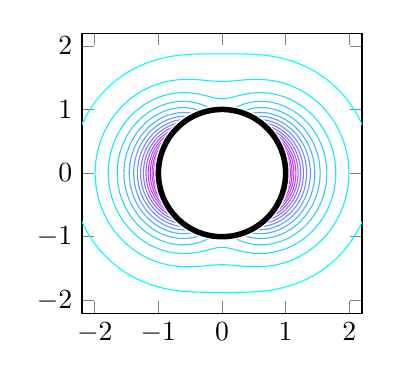
\begin{tikzpicture}

\begin{axis}[%
width=1.4in,
height=1.4in,
at={(0in,0in)},
scale only axis,
colormap={mymap}{[1pt] rgb(0pt)=(0,1,1); rgb(63pt)=(1,0,1)},
xmin=-2.2000,
xmax=2.2000,
ymin=-2.2000,
ymax=2.2000,
axis background/.style={fill=white}
]
\addplot[contour prepared, contour prepared format=matlab, contour/labels=false] table[row sep=crcr] {%
%
0.0556	336.0000\\
2.3637	0.0000\\
2.3619	0.0829\\
2.3564	0.1657\\
2.3545	0.1823\\
2.3473	0.2481\\
2.3346	0.3300\\
2.3183	0.4111\\
2.2984	0.4914\\
2.2930	0.5097\\
2.2751	0.5706\\
2.2484	0.6485\\
2.2322	0.6896\\
2.2183	0.7251\\
2.1849	0.8001\\
2.1722	0.8256\\
2.1484	0.8734\\
2.1129	0.9372\\
2.1087	0.9448\\
2.0661	1.0142\\
2.0542	1.0317\\
2.0205	1.0814\\
1.9962	1.1142\\
1.9722	1.1464\\
1.9389	1.1873\\
1.9213	1.2089\\
1.8822	1.2528\\
1.8679	1.2689\\
1.8261	1.3118\\
1.8121	1.3263\\
1.7706	1.3653\\
1.7540	1.3809\\
1.7157	1.4140\\
1.6940	1.4327\\
1.6613	1.4585\\
1.6320	1.4816\\
1.6075	1.4993\\
1.5683	1.5275\\
1.5542	1.5368\\
1.5029	1.5704\\
1.5016	1.5712\\
1.4490	1.6027\\
1.4363	1.6102\\
1.3969	1.6316\\
1.3684	1.6470\\
1.3453	1.6583\\
1.2994	1.6806\\
1.2943	1.6829\\
1.2432	1.7053\\
1.2296	1.7112\\
1.1924	1.7258\\
1.1590	1.7387\\
1.1419	1.7447\\
1.0918	1.7619\\
1.0880	1.7632\\
1.0412	1.7775\\
1.0166	1.7849\\
0.9909	1.7917\\
0.9450	1.8036\\
0.9409	1.8045\\
0.8900	1.8160\\
0.8735	1.8197\\
0.8389	1.8263\\
0.8021	1.8331\\
0.7876	1.8354\\
0.7357	1.8435\\
0.7309	1.8442\\
0.6821	1.8504\\
0.6602	1.8531\\
0.6273	1.8564\\
0.5899	1.8600\\
0.5710	1.8614\\
0.5203	1.8651\\
0.5121	1.8655\\
0.4512	1.8687\\
0.4495	1.8688\\
0.3829	1.8712\\
0.3805	1.8712\\
0.3152	1.8727\\
0.3004	1.8729\\
0.2480	1.8735\\
0.1982	1.8737\\
0.1814	1.8738\\
0.1153	1.8740\\
0.0493	1.8740\\
-0.0164	1.8740\\
-0.0823	1.8740\\
-0.1483	1.8739\\
-0.1983	1.8737\\
-0.2147	1.8737\\
-0.2815	1.8731\\
-0.3002	1.8729\\
-0.3489	1.8720\\
-0.3793	1.8712\\
-0.4170	1.8701\\
-0.4484	1.8688\\
-0.4857	1.8671\\
-0.5116	1.8655\\
-0.5550	1.8627\\
-0.5710	1.8614\\
-0.6250	1.8567\\
-0.6280	1.8564\\
-0.6822	1.8504\\
-0.6955	1.8489\\
-0.7352	1.8434\\
-0.7665	1.8390\\
-0.7875	1.8354\\
-0.8377	1.8267\\
-0.8394	1.8263\\
-0.8900	1.8160\\
-0.9093	1.8120\\
-0.9405	1.8045\\
-0.9808	1.7946\\
-0.9911	1.7917\\
-1.0414	1.7775\\
-1.0523	1.7744\\
-1.0915	1.7619\\
-1.1236	1.7514\\
-1.1419	1.7447\\
-1.1927	1.7259\\
-1.1944	1.7253\\
-1.2431	1.7053\\
-1.2646	1.6963\\
-1.2940	1.6828\\
-1.3340	1.6642\\
-1.3454	1.6583\\
-1.3971	1.6317\\
-1.4024	1.6290\\
-1.4489	1.6026\\
-1.4698	1.5907\\
-1.5013	1.5710\\
-1.5358	1.5493\\
-1.5542	1.5367\\
-1.6003	1.5049\\
-1.6076	1.4994\\
-1.6615	1.4588\\
-1.6632	1.4575\\
-1.7158	1.4142\\
-1.7242	1.4072\\
-1.7707	1.3654\\
-1.7833	1.3539\\
-1.8261	1.3119\\
-1.8402	1.2979\\
-1.8822	1.2529\\
-1.8949	1.2392\\
-1.9389	1.1875\\
-1.9471	1.1779\\
-1.9963	1.1147\\
-1.9967	1.1142\\
-2.0436	1.0481\\
-2.0542	1.0317\\
-2.0878	0.9797\\
-2.1128	0.9368\\
-2.1289	0.9093\\
-2.1670	0.8369\\
-2.1722	0.8260\\
-2.2020	0.7628\\
-2.2323	0.6905\\
-2.2337	0.6870\\
-2.2622	0.6097\\
-2.2872	0.5311\\
-2.2930	0.5096\\
-2.3088	0.4514\\
-2.3269	0.3706\\
-2.3414	0.2891\\
-2.3523	0.2070\\
-2.3545	0.1813\\
-2.3596	0.1244\\
-2.3632	0.0415\\
-2.3632	-0.0415\\
-2.3596	-0.1244\\
-2.3545	-0.1813\\
-2.3523	-0.2070\\
-2.3414	-0.2891\\
-2.3269	-0.3706\\
-2.3088	-0.4514\\
-2.2930	-0.5096\\
-2.2872	-0.5311\\
-2.2622	-0.6097\\
-2.2337	-0.6870\\
-2.2323	-0.6905\\
-2.2020	-0.7628\\
-2.1722	-0.8260\\
-2.1670	-0.8369\\
-2.1289	-0.9093\\
-2.1128	-0.9368\\
-2.0878	-0.9797\\
-2.0542	-1.0317\\
-2.0436	-1.0481\\
-1.9967	-1.1142\\
-1.9963	-1.1147\\
-1.9471	-1.1779\\
-1.9389	-1.1875\\
-1.8949	-1.2392\\
-1.8822	-1.2529\\
-1.8402	-1.2979\\
-1.8261	-1.3119\\
-1.7833	-1.3539\\
-1.7707	-1.3654\\
-1.7242	-1.4072\\
-1.7158	-1.4142\\
-1.6632	-1.4575\\
-1.6615	-1.4588\\
-1.6076	-1.4994\\
-1.6003	-1.5049\\
-1.5542	-1.5367\\
-1.5358	-1.5493\\
-1.5013	-1.5710\\
-1.4698	-1.5907\\
-1.4489	-1.6026\\
-1.4024	-1.6290\\
-1.3971	-1.6317\\
-1.3454	-1.6583\\
-1.3340	-1.6642\\
-1.2940	-1.6828\\
-1.2646	-1.6963\\
-1.2431	-1.7053\\
-1.1944	-1.7253\\
-1.1927	-1.7259\\
-1.1419	-1.7447\\
-1.1236	-1.7514\\
-1.0915	-1.7619\\
-1.0523	-1.7744\\
-1.0414	-1.7775\\
-0.9911	-1.7917\\
-0.9808	-1.7946\\
-0.9405	-1.8045\\
-0.9093	-1.8120\\
-0.8900	-1.8160\\
-0.8394	-1.8263\\
-0.8377	-1.8267\\
-0.7875	-1.8354\\
-0.7665	-1.8390\\
-0.7352	-1.8434\\
-0.6955	-1.8489\\
-0.6822	-1.8504\\
-0.6280	-1.8564\\
-0.6250	-1.8567\\
-0.5710	-1.8614\\
-0.5550	-1.8627\\
-0.5116	-1.8655\\
-0.4857	-1.8671\\
-0.4484	-1.8688\\
-0.4170	-1.8701\\
-0.3793	-1.8712\\
-0.3489	-1.8720\\
-0.3002	-1.8729\\
-0.2815	-1.8731\\
-0.2147	-1.8737\\
-0.1983	-1.8737\\
-0.1483	-1.8739\\
-0.0823	-1.8740\\
-0.0164	-1.8740\\
0.0493	-1.8740\\
0.1153	-1.8740\\
0.1814	-1.8738\\
0.1982	-1.8737\\
0.2480	-1.8735\\
0.3004	-1.8729\\
0.3152	-1.8727\\
0.3805	-1.8712\\
0.3829	-1.8712\\
0.4495	-1.8688\\
0.4512	-1.8687\\
0.5121	-1.8655\\
0.5203	-1.8651\\
0.5710	-1.8614\\
0.5899	-1.8600\\
0.6273	-1.8564\\
0.6602	-1.8531\\
0.6821	-1.8504\\
0.7309	-1.8442\\
0.7357	-1.8435\\
0.7876	-1.8354\\
0.8021	-1.8331\\
0.8389	-1.8263\\
0.8735	-1.8197\\
0.8900	-1.8160\\
0.9409	-1.8045\\
0.9450	-1.8036\\
0.9909	-1.7917\\
1.0166	-1.7849\\
1.0412	-1.7775\\
1.0880	-1.7632\\
1.0918	-1.7619\\
1.1419	-1.7447\\
1.1590	-1.7387\\
1.1924	-1.7258\\
1.2296	-1.7112\\
1.2432	-1.7053\\
1.2943	-1.6829\\
1.2994	-1.6806\\
1.3453	-1.6583\\
1.3684	-1.6470\\
1.3969	-1.6316\\
1.4363	-1.6102\\
1.4490	-1.6027\\
1.5016	-1.5712\\
1.5029	-1.5704\\
1.5542	-1.5368\\
1.5683	-1.5275\\
1.6075	-1.4993\\
1.6320	-1.4816\\
1.6613	-1.4585\\
1.6940	-1.4327\\
1.7157	-1.4140\\
1.7540	-1.3809\\
1.7706	-1.3653\\
1.8121	-1.3263\\
1.8261	-1.3118\\
1.8679	-1.2689\\
1.8822	-1.2528\\
1.9213	-1.2089\\
1.9389	-1.1873\\
1.9722	-1.1464\\
1.9962	-1.1142\\
2.0205	-1.0814\\
2.0542	-1.0317\\
2.0661	-1.0142\\
2.1087	-0.9448\\
2.1129	-0.9372\\
2.1484	-0.8734\\
2.1722	-0.8256\\
2.1849	-0.8001\\
2.2183	-0.7251\\
2.2322	-0.6896\\
2.2484	-0.6485\\
2.2751	-0.5706\\
2.2930	-0.5097\\
2.2984	-0.4914\\
2.3183	-0.4111\\
2.3346	-0.3300\\
2.3473	-0.2481\\
2.3545	-0.1823\\
2.3564	-0.1657\\
2.3619	-0.0829\\
2.3637	-0.0000\\
0.0556	180.0000\\
0.9932	-0.0000\\
0.9925	-0.0349\\
0.9907	-0.0697\\
0.9877	-0.1044\\
0.9834	-0.1390\\
0.9779	-0.1734\\
0.9712	-0.2076\\
0.9634	-0.2416\\
0.9543	-0.2753\\
0.9441	-0.3086\\
0.9327	-0.3415\\
0.9201	-0.3741\\
0.9064	-0.4061\\
0.8917	-0.4377\\
0.8758	-0.4687\\
0.8588	-0.4992\\
0.8408	-0.5290\\
0.8217	-0.5582\\
0.8016	-0.5867\\
0.7806	-0.6145\\
0.7586	-0.6416\\
0.7356	-0.6678\\
0.7118	-0.6933\\
0.6870	-0.7179\\
0.6615	-0.7416\\
0.6351	-0.7644\\
0.6079	-0.7863\\
0.5800	-0.8072\\
0.5513	-0.8271\\
0.5220	-0.8460\\
0.4921	-0.8639\\
0.4615	-0.8807\\
0.4303	-0.8965\\
0.3987	-0.9112\\
0.3665	-0.9247\\
0.3339	-0.9371\\
0.3008	-0.9484\\
0.2674	-0.9585\\
0.2336	-0.9675\\
0.1995	-0.9752\\
0.1652	-0.9817\\
0.1307	-0.9871\\
0.0960	-0.9911\\
0.0611	-0.9940\\
0.0262	-0.9955\\
-0.0087	-0.9958\\
-0.0437	-0.9949\\
-0.0786	-0.9927\\
-0.1133	-0.9892\\
-0.1480	-0.9846\\
-0.1824	-0.9786\\
-0.2166	-0.9715\\
-0.2505	-0.9632\\
-0.2841	-0.9536\\
-0.3174	-0.9429\\
-0.3502	-0.9311\\
-0.3826	-0.9181\\
-0.4146	-0.9040\\
-0.4460	-0.8888\\
-0.4768	-0.8725\\
-0.5071	-0.8551\\
-0.5368	-0.8367\\
-0.5657	-0.8173\\
-0.5940	-0.7968\\
-0.6216	-0.7754\\
-0.6484	-0.7531\\
-0.6744	-0.7298\\
-0.6995	-0.7057\\
-0.7238	-0.6807\\
-0.7472	-0.6548\\
-0.7697	-0.6282\\
-0.7912	-0.6007\\
-0.8118	-0.5726\\
-0.8314	-0.5437\\
-0.8499	-0.5142\\
-0.8674	-0.4840\\
-0.8838	-0.4533\\
-0.8992	-0.4220\\
-0.9134	-0.3901\\
-0.9265	-0.3578\\
-0.9385	-0.3251\\
-0.9493	-0.2920\\
-0.9590	-0.2585\\
-0.9675	-0.2246\\
-0.9747	-0.1906\\
-0.9808	-0.1562\\
-0.9857	-0.1217\\
-0.9893	-0.0870\\
-0.9918	-0.0523\\
-0.9930	-0.0174\\
-0.9930	0.0174\\
-0.9918	0.0523\\
-0.9893	0.0870\\
-0.9857	0.1217\\
-0.9808	0.1562\\
-0.9747	0.1906\\
-0.9675	0.2246\\
-0.9590	0.2585\\
-0.9493	0.2920\\
-0.9385	0.3251\\
-0.9265	0.3578\\
-0.9134	0.3901\\
-0.8992	0.4220\\
-0.8838	0.4533\\
-0.8674	0.4840\\
-0.8499	0.5142\\
-0.8314	0.5437\\
-0.8118	0.5726\\
-0.7912	0.6007\\
-0.7697	0.6282\\
-0.7472	0.6548\\
-0.7238	0.6807\\
-0.6995	0.7057\\
-0.6744	0.7298\\
-0.6484	0.7531\\
-0.6216	0.7754\\
-0.5940	0.7968\\
-0.5657	0.8173\\
-0.5368	0.8367\\
-0.5071	0.8551\\
-0.4768	0.8725\\
-0.4460	0.8888\\
-0.4146	0.9040\\
-0.3826	0.9181\\
-0.3502	0.9311\\
-0.3174	0.9429\\
-0.2841	0.9536\\
-0.2505	0.9632\\
-0.2166	0.9715\\
-0.1824	0.9786\\
-0.1480	0.9846\\
-0.1133	0.9892\\
-0.0786	0.9927\\
-0.0437	0.9949\\
-0.0087	0.9958\\
0.0262	0.9955\\
0.0611	0.9940\\
0.0960	0.9911\\
0.1307	0.9871\\
0.1652	0.9817\\
0.1995	0.9752\\
0.2336	0.9675\\
0.2674	0.9585\\
0.3008	0.9484\\
0.3339	0.9371\\
0.3665	0.9247\\
0.3987	0.9112\\
0.4303	0.8965\\
0.4615	0.8807\\
0.4921	0.8639\\
0.5220	0.8460\\
0.5513	0.8271\\
0.5800	0.8072\\
0.6079	0.7863\\
0.6351	0.7644\\
0.6615	0.7416\\
0.6870	0.7179\\
0.7118	0.6933\\
0.7356	0.6678\\
0.7586	0.6416\\
0.7806	0.6145\\
0.8016	0.5867\\
0.8217	0.5582\\
0.8408	0.5290\\
0.8588	0.4992\\
0.8758	0.4687\\
0.8917	0.4377\\
0.9064	0.4061\\
0.9201	0.3741\\
0.9327	0.3415\\
0.9441	0.3086\\
0.9543	0.2753\\
0.9634	0.2416\\
0.9712	0.2076\\
0.9779	0.1734\\
0.9834	0.1390\\
0.9877	0.1044\\
0.9907	0.0697\\
0.9925	0.0349\\
0.9932	0.0000\\
0.1111	356.0000\\
1.9939	0.0000\\
1.9923	0.0700\\
1.9875	0.1398\\
1.9795	0.2092\\
1.9683	0.2782\\
1.9558	0.3378\\
1.9540	0.3465\\
1.9366	0.4140\\
1.9162	0.4805\\
1.9031	0.5169\\
1.8927	0.5459\\
1.8663	0.6100\\
1.8512	0.6424\\
1.8371	0.6727\\
1.8050	0.7338\\
1.8000	0.7423\\
1.7703	0.7932\\
1.7496	0.8250\\
1.7330	0.8507\\
1.7000	0.8967\\
1.6931	0.9062\\
1.6510	0.9594\\
1.6509	0.9596\\
1.6064	1.0108\\
1.6028	1.0146\\
1.5597	1.0596\\
1.5552	1.0639\\
1.5111	1.1060\\
1.5084	1.1083\\
1.4622	1.1484\\
1.4605	1.1498\\
1.4166	1.1845\\
1.4083	1.1911\\
1.3717	1.2173\\
1.3544	1.2296\\
1.3274	1.2471\\
1.2991	1.2653\\
1.2838	1.2742\\
1.2424	1.2982\\
1.2409	1.2990\\
1.1983	1.3212\\
1.1847	1.3282\\
1.1564	1.3415\\
1.1261	1.3554\\
1.1151	1.3599\\
1.0744	1.3764\\
1.0666	1.3796\\
1.0339	1.3913\\
1.0066	1.4009\\
0.9942	1.4047\\
0.9550	1.4166\\
0.9461	1.4192\\
0.9159	1.4271\\
0.8853	1.4347\\
0.8776	1.4364\\
0.8395	1.4444\\
0.8244	1.4475\\
0.8017	1.4514\\
0.7647	1.4573\\
0.7637	1.4574\\
0.7272	1.4621\\
0.7032	1.4648\\
0.6905	1.4660\\
0.6538	1.4690\\
0.6431	1.4697\\
0.6171	1.4711\\
0.5835	1.4723\\
0.5810	1.4724\\
0.5440	1.4729\\
0.5247	1.4729\\
0.5073	1.4727\\
0.4706	1.4718\\
0.4668	1.4716\\
0.4325	1.4701\\
0.4097	1.4689\\
0.3942	1.4679\\
0.3552	1.4651\\
0.3537	1.4649\\
0.3132	1.4616\\
0.2988	1.4603\\
0.2687	1.4576\\
0.2449	1.4553\\
0.2198	1.4531\\
0.1920	1.4505\\
0.1617	1.4481\\
0.1400	1.4463\\
0.0888	1.4430\\
0.0763	1.4425\\
0.0379	1.4411\\
-0.0126	1.4407\\
-0.0633	1.4419\\
-0.0762	1.4425\\
-0.1143	1.4445\\
-0.1633	1.4481\\
-0.1659	1.4483\\
-0.2184	1.4528\\
-0.2210	1.4531\\
-0.2697	1.4576\\
-0.2717	1.4578\\
-0.3132	1.4616\\
-0.3261	1.4627\\
-0.3544	1.4651\\
-0.3816	1.4670\\
-0.3943	1.4679\\
-0.4330	1.4702\\
-0.4381	1.4704\\
-0.4701	1.4717\\
-0.4956	1.4725\\
-0.5074	1.4727\\
-0.5442	1.4729\\
-0.5540	1.4729\\
-0.5805	1.4724\\
-0.6132	1.4713\\
-0.6174	1.4711\\
-0.6537	1.4689\\
-0.6731	1.4676\\
-0.6904	1.4660\\
-0.7275	1.4621\\
-0.7334	1.4614\\
-0.7643	1.4572\\
-0.7940	1.4528\\
-0.8019	1.4514\\
-0.8395	1.4444\\
-0.8549	1.4415\\
-0.8775	1.4364\\
-0.9157	1.4273\\
-0.9162	1.4272\\
-0.9548	1.4165\\
-0.9764	1.4104\\
-0.9942	1.4047\\
-1.0342	1.3914\\
-1.0366	1.3906\\
-1.0742	1.3764\\
-1.0964	1.3678\\
-1.1151	1.3598\\
-1.1555	1.3421\\
-1.1566	1.3416\\
-1.1983	1.3212\\
-1.2137	1.3136\\
-1.2407	1.2988\\
-1.2709	1.2821\\
-1.2838	1.2742\\
-1.3269	1.2478\\
-1.3276	1.2473\\
-1.3717	1.2173\\
-1.3815	1.2107\\
-1.4166	1.1844\\
-1.4346	1.1708\\
-1.4621	1.1481\\
-1.4861	1.1283\\
-1.5083	1.1081\\
-1.5357	1.0831\\
-1.5552	1.0637\\
-1.5834	1.0355\\
-1.6027	1.0143\\
-1.6289	0.9855\\
-1.6510	0.9589\\
-1.6723	0.9332\\
-1.6999	0.8965\\
-1.7134	0.8787\\
-1.7497	0.8255\\
-1.7519	0.8221\\
-1.7880	0.7637\\
-1.8000	0.7420\\
-1.8214	0.7035\\
-1.8512	0.6432\\
-1.8520	0.6415\\
-1.8799	0.5782\\
-1.9031	0.5177\\
-1.9048	0.5134\\
-1.9268	0.4474\\
-1.9457	0.3804\\
-1.9558	0.3369\\
-1.9616	0.3124\\
-1.9743	0.2438\\
-1.9839	0.1745\\
-1.9903	0.1049\\
-1.9935	0.0350\\
-1.9935	-0.0350\\
-1.9903	-0.1049\\
-1.9839	-0.1745\\
-1.9743	-0.2438\\
-1.9616	-0.3124\\
-1.9558	-0.3369\\
-1.9457	-0.3804\\
-1.9268	-0.4474\\
-1.9048	-0.5134\\
-1.9031	-0.5177\\
-1.8799	-0.5782\\
-1.8520	-0.6415\\
-1.8512	-0.6432\\
-1.8214	-0.7035\\
-1.8000	-0.7420\\
-1.7880	-0.7637\\
-1.7519	-0.8221\\
-1.7497	-0.8255\\
-1.7134	-0.8787\\
-1.6999	-0.8965\\
-1.6723	-0.9332\\
-1.6510	-0.9589\\
-1.6289	-0.9855\\
-1.6027	-1.0143\\
-1.5834	-1.0355\\
-1.5552	-1.0637\\
-1.5357	-1.0831\\
-1.5083	-1.1081\\
-1.4861	-1.1283\\
-1.4621	-1.1481\\
-1.4346	-1.1708\\
-1.4166	-1.1844\\
-1.3815	-1.2107\\
-1.3717	-1.2173\\
-1.3276	-1.2473\\
-1.3269	-1.2478\\
-1.2838	-1.2742\\
-1.2709	-1.2821\\
-1.2407	-1.2988\\
-1.2137	-1.3136\\
-1.1983	-1.3212\\
-1.1566	-1.3416\\
-1.1555	-1.3421\\
-1.1151	-1.3598\\
-1.0964	-1.3678\\
-1.0742	-1.3764\\
-1.0366	-1.3906\\
-1.0342	-1.3914\\
-0.9942	-1.4047\\
-0.9764	-1.4104\\
-0.9548	-1.4165\\
-0.9162	-1.4272\\
-0.9157	-1.4273\\
-0.8775	-1.4364\\
-0.8549	-1.4415\\
-0.8395	-1.4444\\
-0.8019	-1.4514\\
-0.7940	-1.4528\\
-0.7643	-1.4572\\
-0.7334	-1.4614\\
-0.7275	-1.4621\\
-0.6904	-1.4660\\
-0.6731	-1.4676\\
-0.6537	-1.4689\\
-0.6174	-1.4711\\
-0.6132	-1.4713\\
-0.5805	-1.4724\\
-0.5540	-1.4729\\
-0.5442	-1.4729\\
-0.5074	-1.4727\\
-0.4956	-1.4725\\
-0.4701	-1.4717\\
-0.4381	-1.4704\\
-0.4330	-1.4702\\
-0.3943	-1.4679\\
-0.3816	-1.4670\\
-0.3544	-1.4651\\
-0.3261	-1.4627\\
-0.3132	-1.4616\\
-0.2717	-1.4578\\
-0.2697	-1.4576\\
-0.2210	-1.4531\\
-0.2184	-1.4528\\
-0.1659	-1.4483\\
-0.1633	-1.4481\\
-0.1143	-1.4445\\
-0.0762	-1.4425\\
-0.0633	-1.4419\\
-0.0126	-1.4407\\
0.0379	-1.4411\\
0.0763	-1.4425\\
0.0888	-1.4430\\
0.1400	-1.4463\\
0.1617	-1.4481\\
0.1920	-1.4505\\
0.2198	-1.4531\\
0.2449	-1.4553\\
0.2687	-1.4576\\
0.2988	-1.4603\\
0.3132	-1.4616\\
0.3537	-1.4649\\
0.3552	-1.4651\\
0.3942	-1.4679\\
0.4097	-1.4689\\
0.4325	-1.4701\\
0.4668	-1.4716\\
0.4706	-1.4718\\
0.5073	-1.4727\\
0.5247	-1.4729\\
0.5440	-1.4729\\
0.5810	-1.4724\\
0.5835	-1.4723\\
0.6171	-1.4711\\
0.6431	-1.4697\\
0.6538	-1.4690\\
0.6905	-1.4660\\
0.7032	-1.4648\\
0.7272	-1.4621\\
0.7637	-1.4574\\
0.7647	-1.4573\\
0.8017	-1.4514\\
0.8244	-1.4475\\
0.8395	-1.4444\\
0.8776	-1.4364\\
0.8853	-1.4347\\
0.9159	-1.4271\\
0.9461	-1.4192\\
0.9550	-1.4166\\
0.9942	-1.4047\\
1.0066	-1.4009\\
1.0339	-1.3913\\
1.0666	-1.3796\\
1.0744	-1.3764\\
1.1151	-1.3599\\
1.1261	-1.3554\\
1.1564	-1.3415\\
1.1847	-1.3282\\
1.1983	-1.3212\\
1.2409	-1.2990\\
1.2424	-1.2982\\
1.2838	-1.2742\\
1.2991	-1.2653\\
1.3274	-1.2471\\
1.3544	-1.2296\\
1.3717	-1.2173\\
1.4083	-1.1911\\
1.4166	-1.1845\\
1.4605	-1.1498\\
1.4622	-1.1484\\
1.5084	-1.1083\\
1.5111	-1.1060\\
1.5552	-1.0639\\
1.5597	-1.0596\\
1.6028	-1.0146\\
1.6064	-1.0108\\
1.6509	-0.9596\\
1.6510	-0.9594\\
1.6931	-0.9062\\
1.7000	-0.8967\\
1.7330	-0.8507\\
1.7496	-0.8250\\
1.7703	-0.7932\\
1.8000	-0.7423\\
1.8050	-0.7338\\
1.8371	-0.6727\\
1.8512	-0.6424\\
1.8663	-0.6100\\
1.8927	-0.5459\\
1.9031	-0.5169\\
1.9162	-0.4805\\
1.9366	-0.4140\\
1.9540	-0.3465\\
1.9558	-0.3378\\
1.9683	-0.2782\\
1.9795	-0.2092\\
1.9875	-0.1398\\
1.9923	-0.0700\\
1.9939	-0.0000\\
0.1111	180.0000\\
0.9939	-0.0000\\
0.9932	-0.0349\\
0.9914	-0.0697\\
0.9884	-0.1045\\
0.9841	-0.1391\\
0.9786	-0.1735\\
0.9719	-0.2078\\
0.9641	-0.2418\\
0.9550	-0.2755\\
0.9448	-0.3088\\
0.9334	-0.3418\\
0.9209	-0.3743\\
0.9072	-0.4064\\
0.8924	-0.4381\\
0.8765	-0.4691\\
0.8596	-0.4996\\
0.8415	-0.5295\\
0.8225	-0.5588\\
0.8024	-0.5873\\
0.7814	-0.6152\\
0.7594	-0.6423\\
0.7364	-0.6686\\
0.7126	-0.6941\\
0.6879	-0.7187\\
0.6623	-0.7425\\
0.6359	-0.7654\\
0.6087	-0.7874\\
0.5808	-0.8084\\
0.5522	-0.8284\\
0.5229	-0.8474\\
0.4929	-0.8654\\
0.4624	-0.8824\\
0.4312	-0.8983\\
0.3995	-0.9131\\
0.3673	-0.9268\\
0.3347	-0.9394\\
0.3016	-0.9508\\
0.2681	-0.9611\\
0.2343	-0.9702\\
0.2001	-0.9781\\
0.1657	-0.9848\\
0.1311	-0.9902\\
0.0963	-0.9944\\
0.0613	-0.9973\\
0.0263	-0.9989\\
-0.0088	-0.9993\\
-0.0438	-0.9983\\
-0.0788	-0.9960\\
-0.1137	-0.9925\\
-0.1484	-0.9877\\
-0.1830	-0.9816\\
-0.2172	-0.9743\\
-0.2512	-0.9658\\
-0.2849	-0.9561\\
-0.3182	-0.9452\\
-0.3510	-0.9332\\
-0.3835	-0.9201\\
-0.4154	-0.9058\\
-0.4468	-0.8905\\
-0.4777	-0.8740\\
-0.5080	-0.8566\\
-0.5376	-0.8380\\
-0.5666	-0.8185\\
-0.5949	-0.7980\\
-0.6224	-0.7765\\
-0.6492	-0.7541\\
-0.6752	-0.7307\\
-0.7003	-0.7065\\
-0.7246	-0.6814\\
-0.7480	-0.6555\\
-0.7705	-0.6288\\
-0.7920	-0.6013\\
-0.8126	-0.5731\\
-0.8321	-0.5442\\
-0.8507	-0.5146\\
-0.8682	-0.4844\\
-0.8846	-0.4537\\
-0.8999	-0.4223\\
-0.9142	-0.3905\\
-0.9273	-0.3581\\
-0.9392	-0.3254\\
-0.9500	-0.2922\\
-0.9597	-0.2587\\
-0.9682	-0.2248\\
-0.9754	-0.1907\\
-0.9815	-0.1563\\
-0.9864	-0.1218\\
-0.9900	-0.0871\\
-0.9925	-0.0523\\
-0.9937	-0.0174\\
-0.9937	0.0174\\
-0.9925	0.0523\\
-0.9900	0.0871\\
-0.9864	0.1218\\
-0.9815	0.1563\\
-0.9754	0.1907\\
-0.9682	0.2248\\
-0.9597	0.2587\\
-0.9500	0.2922\\
-0.9392	0.3254\\
-0.9273	0.3581\\
-0.9142	0.3905\\
-0.8999	0.4223\\
-0.8846	0.4537\\
-0.8682	0.4844\\
-0.8507	0.5146\\
-0.8321	0.5442\\
-0.8126	0.5731\\
-0.7920	0.6013\\
-0.7705	0.6288\\
-0.7480	0.6555\\
-0.7246	0.6814\\
-0.7003	0.7065\\
-0.6752	0.7307\\
-0.6492	0.7541\\
-0.6224	0.7765\\
-0.5949	0.7980\\
-0.5666	0.8185\\
-0.5376	0.8380\\
-0.5080	0.8566\\
-0.4777	0.8740\\
-0.4468	0.8905\\
-0.4154	0.9058\\
-0.3835	0.9201\\
-0.3510	0.9332\\
-0.3182	0.9452\\
-0.2849	0.9561\\
-0.2512	0.9658\\
-0.2172	0.9743\\
-0.1830	0.9816\\
-0.1484	0.9877\\
-0.1137	0.9925\\
-0.0788	0.9960\\
-0.0438	0.9983\\
-0.0088	0.9993\\
0.0263	0.9989\\
0.0613	0.9973\\
0.0963	0.9944\\
0.1311	0.9902\\
0.1657	0.9848\\
0.2001	0.9781\\
0.2343	0.9702\\
0.2681	0.9611\\
0.3016	0.9508\\
0.3347	0.9394\\
0.3673	0.9268\\
0.3995	0.9131\\
0.4312	0.8983\\
0.4624	0.8824\\
0.4929	0.8654\\
0.5229	0.8474\\
0.5522	0.8284\\
0.5808	0.8084\\
0.6087	0.7874\\
0.6359	0.7654\\
0.6623	0.7425\\
0.6879	0.7187\\
0.7126	0.6941\\
0.7364	0.6686\\
0.7594	0.6423\\
0.7814	0.6152\\
0.8024	0.5873\\
0.8225	0.5588\\
0.8415	0.5295\\
0.8596	0.4996\\
0.8765	0.4691\\
0.8924	0.4381\\
0.9072	0.4064\\
0.9209	0.3743\\
0.9334	0.3418\\
0.9448	0.3088\\
0.9550	0.2755\\
0.9641	0.2418\\
0.9719	0.2078\\
0.9786	0.1735\\
0.9841	0.1391\\
0.9884	0.1045\\
0.9914	0.0697\\
0.9932	0.0349\\
0.9939	0.0000\\
0.1667	380.0000\\
1.7880	0.0000\\
1.7865	0.0627\\
1.7821	0.1253\\
1.7747	0.1876\\
1.7721	0.2033\\
1.7644	0.2494\\
1.7513	0.3106\\
1.7352	0.3710\\
1.7236	0.4076\\
1.7163	0.4304\\
1.6947	0.4888\\
1.6758	0.5332\\
1.6704	0.5460\\
1.6435	0.6018\\
1.6289	0.6286\\
1.6139	0.6561\\
1.5827	0.7074\\
1.5819	0.7088\\
1.5476	0.7597\\
1.5373	0.7734\\
1.5109	0.8087\\
1.4926	0.8308\\
1.4721	0.8557\\
1.4487	0.8813\\
1.4312	0.9005\\
1.4055	0.9260\\
1.3883	0.9431\\
1.3631	0.9659\\
1.3436	0.9834\\
1.3213	1.0016\\
1.2972	1.0212\\
1.2803	1.0337\\
1.2492	1.0565\\
1.2400	1.0626\\
1.2004	1.0887\\
1.1997	1.0892\\
1.1613	1.1120\\
1.1491	1.1192\\
1.1229	1.1330\\
1.0972	1.1464\\
1.0853	1.1520\\
1.0483	1.1691\\
1.0444	1.1709\\
1.0118	1.1842\\
0.9908	1.1925\\
0.9760	1.1977\\
0.9409	1.2098\\
0.9365	1.2113\\
0.9061	1.2202\\
0.8817	1.2271\\
0.8722	1.2295\\
0.8387	1.2374\\
0.8266	1.2401\\
0.8057	1.2441\\
0.7736	1.2498\\
0.7714	1.2502\\
0.7415	1.2543\\
0.7162	1.2574\\
0.7103	1.2579\\
0.6793	1.2606\\
0.6612	1.2618\\
0.6490	1.2624\\
0.6191	1.2633\\
0.6065	1.2636\\
0.5896	1.2635\\
0.5607	1.2629\\
0.5525	1.2626\\
0.5319	1.2616\\
0.5040	1.2596\\
0.4991	1.2593\\
0.4757	1.2570\\
0.4485	1.2538\\
0.4466	1.2536\\
0.4207	1.2500\\
0.3951	1.2458\\
0.3941	1.2457\\
0.3666	1.2408\\
0.3449	1.2364\\
0.3401	1.2354\\
0.3127	1.2295\\
0.2959	1.2255\\
0.2858	1.2232\\
0.2583	1.2165\\
0.2484	1.2138\\
0.2299	1.2093\\
0.2023	1.2019\\
0.2017	1.2018\\
0.1700	1.1938\\
0.1576	1.1905\\
0.1355	1.1856\\
0.1143	1.1805\\
0.0944	1.1769\\
0.0721	1.1728\\
0.0308	1.1682\\
0.0238	1.1680\\
-0.0102	1.1672\\
-0.0216	1.1680\\
-0.0514	1.1700\\
-0.0931	1.1763\\
-0.0961	1.1769\\
-0.1358	1.1853\\
-0.1369	1.1856\\
-0.1701	1.1938\\
-0.1798	1.1961\\
-0.2007	1.2018\\
-0.2251	1.2079\\
-0.2304	1.2093\\
-0.2581	1.2165\\
-0.2720	1.2198\\
-0.2856	1.2232\\
-0.3130	1.2295\\
-0.3202	1.2311\\
-0.3396	1.2354\\
-0.3671	1.2408\\
-0.3699	1.2413\\
-0.3936	1.2456\\
-0.4207	1.2499\\
-0.4213	1.2500\\
-0.4481	1.2538\\
-0.4727	1.2567\\
-0.4761	1.2570\\
-0.5036	1.2596\\
-0.5257	1.2612\\
-0.5322	1.2616\\
-0.5606	1.2629\\
-0.5794	1.2634\\
-0.5897	1.2635\\
-0.6191	1.2633\\
-0.6338	1.2630\\
-0.6490	1.2624\\
-0.6794	1.2606\\
-0.6886	1.2600\\
-0.7101	1.2579\\
-0.7417	1.2544\\
-0.7438	1.2541\\
-0.7733	1.2497\\
-0.7990	1.2455\\
-0.8058	1.2441\\
-0.8386	1.2374\\
-0.8542	1.2340\\
-0.8721	1.2294\\
-0.9063	1.2203\\
-0.9091	1.2195\\
-0.9407	1.2097\\
-0.9637	1.2023\\
-0.9760	1.1978\\
-1.0119	1.1843\\
-1.0177	1.1821\\
-1.0482	1.1690\\
-1.0709	1.1590\\
-1.0853	1.1520\\
-1.1231	1.1332\\
-1.1232	1.1331\\
-1.1613	1.1120\\
-1.1746	1.1045\\
-1.2003	1.0885\\
-1.2246	1.0732\\
-1.2400	1.0625\\
-1.2733	1.0392\\
-1.2804	1.0338\\
-1.3205	1.0026\\
-1.3215	1.0018\\
-1.3632	0.9661\\
-1.3661	0.9635\\
-1.4056	0.9262\\
-1.4099	0.9221\\
-1.4488	0.8816\\
-1.4519	0.8783\\
-1.4917	0.8324\\
-1.4927	0.8312\\
-1.5295	0.7844\\
-1.5373	0.7735\\
-1.5651	0.7345\\
-1.5827	0.7069\\
-1.5983	0.6827\\
-1.6289	0.6293\\
-1.6290	0.6291\\
-1.6573	0.5741\\
-1.6758	0.5331\\
-1.6829	0.5176\\
-1.7059	0.4598\\
-1.7236	0.4082\\
-1.7261	0.4008\\
-1.7436	0.3409\\
-1.7582	0.2801\\
-1.7699	0.2185\\
-1.7721	0.2033\\
-1.7788	0.1565\\
-1.7847	0.0941\\
-1.7877	0.0314\\
-1.7877	-0.0314\\
-1.7847	-0.0941\\
-1.7788	-0.1565\\
-1.7721	-0.2033\\
-1.7699	-0.2185\\
-1.7582	-0.2801\\
-1.7436	-0.3409\\
-1.7261	-0.4008\\
-1.7236	-0.4082\\
-1.7059	-0.4598\\
-1.6829	-0.5176\\
-1.6758	-0.5331\\
-1.6573	-0.5741\\
-1.6290	-0.6291\\
-1.6289	-0.6293\\
-1.5983	-0.6827\\
-1.5827	-0.7069\\
-1.5651	-0.7345\\
-1.5373	-0.7735\\
-1.5295	-0.7844\\
-1.4927	-0.8312\\
-1.4917	-0.8324\\
-1.4519	-0.8783\\
-1.4488	-0.8816\\
-1.4099	-0.9221\\
-1.4056	-0.9262\\
-1.3661	-0.9635\\
-1.3632	-0.9661\\
-1.3215	-1.0018\\
-1.3205	-1.0026\\
-1.2804	-1.0338\\
-1.2733	-1.0392\\
-1.2400	-1.0625\\
-1.2246	-1.0732\\
-1.2003	-1.0885\\
-1.1746	-1.1045\\
-1.1613	-1.1120\\
-1.1232	-1.1331\\
-1.1231	-1.1332\\
-1.0853	-1.1520\\
-1.0709	-1.1590\\
-1.0482	-1.1690\\
-1.0177	-1.1821\\
-1.0119	-1.1843\\
-0.9760	-1.1978\\
-0.9637	-1.2023\\
-0.9407	-1.2097\\
-0.9091	-1.2195\\
-0.9063	-1.2203\\
-0.8721	-1.2294\\
-0.8542	-1.2340\\
-0.8386	-1.2374\\
-0.8058	-1.2441\\
-0.7990	-1.2455\\
-0.7733	-1.2497\\
-0.7438	-1.2541\\
-0.7417	-1.2544\\
-0.7101	-1.2579\\
-0.6886	-1.2600\\
-0.6794	-1.2606\\
-0.6490	-1.2624\\
-0.6338	-1.2630\\
-0.6191	-1.2633\\
-0.5897	-1.2635\\
-0.5794	-1.2634\\
-0.5606	-1.2629\\
-0.5322	-1.2616\\
-0.5257	-1.2612\\
-0.5036	-1.2596\\
-0.4761	-1.2570\\
-0.4727	-1.2567\\
-0.4481	-1.2538\\
-0.4213	-1.2500\\
-0.4207	-1.2499\\
-0.3936	-1.2456\\
-0.3699	-1.2413\\
-0.3671	-1.2408\\
-0.3396	-1.2354\\
-0.3202	-1.2311\\
-0.3130	-1.2295\\
-0.2856	-1.2232\\
-0.2720	-1.2198\\
-0.2581	-1.2165\\
-0.2304	-1.2093\\
-0.2251	-1.2079\\
-0.2007	-1.2018\\
-0.1798	-1.1961\\
-0.1701	-1.1938\\
-0.1369	-1.1856\\
-0.1358	-1.1853\\
-0.0961	-1.1769\\
-0.0931	-1.1763\\
-0.0514	-1.1700\\
-0.0216	-1.1680\\
-0.0102	-1.1672\\
0.0238	-1.1680\\
0.0308	-1.1682\\
0.0721	-1.1728\\
0.0944	-1.1769\\
0.1143	-1.1805\\
0.1355	-1.1856\\
0.1576	-1.1905\\
0.1700	-1.1938\\
0.2017	-1.2018\\
0.2023	-1.2019\\
0.2299	-1.2093\\
0.2484	-1.2138\\
0.2583	-1.2165\\
0.2858	-1.2232\\
0.2959	-1.2255\\
0.3127	-1.2295\\
0.3401	-1.2354\\
0.3449	-1.2364\\
0.3666	-1.2408\\
0.3941	-1.2457\\
0.3951	-1.2458\\
0.4207	-1.2500\\
0.4466	-1.2536\\
0.4485	-1.2538\\
0.4757	-1.2570\\
0.4991	-1.2593\\
0.5040	-1.2596\\
0.5319	-1.2616\\
0.5525	-1.2626\\
0.5607	-1.2629\\
0.5896	-1.2635\\
0.6065	-1.2636\\
0.6191	-1.2633\\
0.6490	-1.2624\\
0.6612	-1.2618\\
0.6793	-1.2606\\
0.7103	-1.2579\\
0.7162	-1.2574\\
0.7415	-1.2543\\
0.7714	-1.2502\\
0.7736	-1.2498\\
0.8057	-1.2441\\
0.8266	-1.2401\\
0.8387	-1.2374\\
0.8722	-1.2295\\
0.8817	-1.2271\\
0.9061	-1.2202\\
0.9365	-1.2113\\
0.9409	-1.2098\\
0.9760	-1.1977\\
0.9908	-1.1925\\
1.0118	-1.1842\\
1.0444	-1.1709\\
1.0483	-1.1691\\
1.0853	-1.1520\\
1.0972	-1.1464\\
1.1229	-1.1330\\
1.1491	-1.1192\\
1.1613	-1.1120\\
1.1997	-1.0892\\
1.2004	-1.0887\\
1.2400	-1.0626\\
1.2492	-1.0565\\
1.2803	-1.0337\\
1.2972	-1.0212\\
1.3213	-1.0016\\
1.3436	-0.9834\\
1.3631	-0.9659\\
1.3883	-0.9431\\
1.4055	-0.9260\\
1.4312	-0.9005\\
1.4487	-0.8813\\
1.4721	-0.8557\\
1.4926	-0.8308\\
1.5109	-0.8087\\
1.5373	-0.7734\\
1.5476	-0.7597\\
1.5819	-0.7088\\
1.5827	-0.7074\\
1.6139	-0.6561\\
1.6289	-0.6286\\
1.6435	-0.6018\\
1.6704	-0.5460\\
1.6758	-0.5332\\
1.6947	-0.4888\\
1.7163	-0.4304\\
1.7236	-0.4076\\
1.7352	-0.3710\\
1.7513	-0.3106\\
1.7644	-0.2494\\
1.7721	-0.2033\\
1.7747	-0.1876\\
1.7821	-0.1253\\
1.7865	-0.0627\\
1.7880	-0.0000\\
0.1667	180.0000\\
0.9946	-0.0000\\
0.9939	-0.0349\\
0.9921	-0.0698\\
0.9891	-0.1045\\
0.9848	-0.1392\\
0.9793	-0.1737\\
0.9727	-0.2079\\
0.9648	-0.2419\\
0.9557	-0.2757\\
0.9455	-0.3090\\
0.9341	-0.3421\\
0.9216	-0.3746\\
0.9079	-0.4068\\
0.8931	-0.4384\\
0.8773	-0.4695\\
0.8603	-0.5001\\
0.8423	-0.5300\\
0.8233	-0.5593\\
0.8032	-0.5879\\
0.7822	-0.6158\\
0.7602	-0.6429\\
0.7372	-0.6693\\
0.7134	-0.6949\\
0.6887	-0.7196\\
0.6631	-0.7434\\
0.6368	-0.7664\\
0.6096	-0.7885\\
0.5817	-0.8096\\
0.5531	-0.8297\\
0.5238	-0.8488\\
0.4938	-0.8669\\
0.4632	-0.8840\\
0.4321	-0.9001\\
0.4004	-0.9150\\
0.3681	-0.9289\\
0.3355	-0.9416\\
0.3023	-0.9532\\
0.2688	-0.9637\\
0.2349	-0.9729\\
0.2007	-0.9810\\
0.1662	-0.9878\\
0.1315	-0.9934\\
0.0966	-0.9977\\
0.0615	-1.0007\\
0.0264	-1.0023\\
-0.0088	-1.0027\\
-0.0440	-1.0017\\
-0.0791	-0.9993\\
-0.1141	-0.9957\\
-0.1489	-0.9908\\
-0.1835	-0.9846\\
-0.2179	-0.9771\\
-0.2519	-0.9685\\
-0.2856	-0.9586\\
-0.3190	-0.9476\\
-0.3519	-0.9354\\
-0.3843	-0.9221\\
-0.4163	-0.9077\\
-0.4477	-0.8922\\
-0.4786	-0.8756\\
-0.5089	-0.8580\\
-0.5385	-0.8394\\
-0.5675	-0.8197\\
-0.5957	-0.7991\\
-0.6233	-0.7776\\
-0.6500	-0.7550\\
-0.6760	-0.7316\\
-0.7012	-0.7073\\
-0.7254	-0.6822\\
-0.7488	-0.6562\\
-0.7713	-0.6294\\
-0.7928	-0.6019\\
-0.8134	-0.5737\\
-0.8329	-0.5447\\
-0.8514	-0.5151\\
-0.8689	-0.4849\\
-0.8853	-0.4540\\
-0.9007	-0.4227\\
-0.9149	-0.3908\\
-0.9280	-0.3584\\
-0.9400	-0.3256\\
-0.9508	-0.2924\\
-0.9604	-0.2588\\
-0.9689	-0.2250\\
-0.9761	-0.1908\\
-0.9822	-0.1565\\
-0.9871	-0.1219\\
-0.9907	-0.0872\\
-0.9932	-0.0523\\
-0.9944	-0.0175\\
-0.9944	0.0175\\
-0.9932	0.0523\\
-0.9907	0.0872\\
-0.9871	0.1219\\
-0.9822	0.1565\\
-0.9761	0.1908\\
-0.9689	0.2250\\
-0.9604	0.2588\\
-0.9508	0.2924\\
-0.9400	0.3256\\
-0.9280	0.3584\\
-0.9149	0.3908\\
-0.9007	0.4227\\
-0.8853	0.4540\\
-0.8689	0.4849\\
-0.8514	0.5151\\
-0.8329	0.5447\\
-0.8134	0.5737\\
-0.7928	0.6019\\
-0.7713	0.6294\\
-0.7488	0.6562\\
-0.7254	0.6822\\
-0.7012	0.7073\\
-0.6760	0.7316\\
-0.6500	0.7550\\
-0.6233	0.7776\\
-0.5957	0.7991\\
-0.5675	0.8197\\
-0.5385	0.8394\\
-0.5089	0.8580\\
-0.4786	0.8756\\
-0.4477	0.8922\\
-0.4163	0.9077\\
-0.3843	0.9221\\
-0.3519	0.9354\\
-0.3190	0.9476\\
-0.2856	0.9586\\
-0.2519	0.9685\\
-0.2179	0.9771\\
-0.1835	0.9846\\
-0.1489	0.9908\\
-0.1141	0.9957\\
-0.0791	0.9993\\
-0.0440	1.0017\\
-0.0088	1.0027\\
0.0264	1.0023\\
0.0615	1.0007\\
0.0966	0.9977\\
0.1315	0.9934\\
0.1662	0.9878\\
0.2007	0.9810\\
0.2349	0.9729\\
0.2688	0.9637\\
0.3023	0.9532\\
0.3355	0.9416\\
0.3681	0.9289\\
0.4004	0.9150\\
0.4321	0.9001\\
0.4632	0.8840\\
0.4938	0.8669\\
0.5238	0.8488\\
0.5531	0.8297\\
0.5817	0.8096\\
0.6096	0.7885\\
0.6368	0.7664\\
0.6631	0.7434\\
0.6887	0.7196\\
0.7134	0.6949\\
0.7372	0.6693\\
0.7602	0.6429\\
0.7822	0.6158\\
0.8032	0.5879\\
0.8233	0.5593\\
0.8423	0.5300\\
0.8603	0.5001\\
0.8773	0.4695\\
0.8931	0.4384\\
0.9079	0.4068\\
0.9216	0.3746\\
0.9341	0.3421\\
0.9455	0.3090\\
0.9557	0.2757\\
0.9648	0.2419\\
0.9727	0.2079\\
0.9793	0.1737\\
0.9848	0.1392\\
0.9891	0.1045\\
0.9921	0.0698\\
0.9939	0.0349\\
0.9946	0.0000\\
0.2222	134.0000\\
1.6474	0.0000\\
1.6460	0.0578\\
1.6418	0.1154\\
1.6414	0.1184\\
1.6348	0.1728\\
1.6252	0.2297\\
1.6127	0.2860\\
1.5976	0.3415\\
1.5957	0.3474\\
1.5799	0.3962\\
1.5595	0.4498\\
1.5508	0.4698\\
1.5366	0.5023\\
1.5112	0.5534\\
1.5066	0.5616\\
1.4835	0.6031\\
1.4633	0.6353\\
1.4534	0.6512\\
1.4210	0.6975\\
1.4208	0.6978\\
1.3865	0.7421\\
1.3790	0.7509\\
1.3500	0.7847\\
1.3380	0.7975\\
1.3116	0.8253\\
1.2977	0.8385\\
1.2713	0.8636\\
1.2582	0.8749\\
1.2292	0.8997\\
1.2194	0.9074\\
1.1856	0.9334\\
1.1813	0.9364\\
1.1440	0.9623\\
1.1406	0.9647\\
1.1073	0.9853\\
1.0942	0.9934\\
1.0713	1.0060\\
1.0466	1.0194\\
1.0361	1.0246\\
1.0016	1.0411\\
0.9980	1.0428\\
0.9675	1.0557\\
0.9485	1.0634\\
0.9343	1.0686\\
0.9018	1.0800\\
0.8983	1.0812\\
0.8697	1.0898\\
0.8475	1.0961\\
0.8384	1.0984\\
0.8077	1.1056\\
0.7962	1.1082\\
0.7775	1.1117\\
0.7482	1.1167\\
0.7447	1.1172\\
0.7192	1.1205\\
0.6931	1.1234\\
0.6911	1.1235\\
0.6632	1.1255\\
0.6416	1.1265\\
0.6363	1.1266\\
0.6095	1.1269\\
0.5904	1.1267\\
0.5837	1.1265\\
0.5581	1.1253\\
0.5395	1.1240\\
0.5334	1.1234\\
0.5089	1.1209\\
0.4893	1.1183\\
0.4853	1.1177\\
0.4618	1.1139\\
0.4398	1.1097\\
0.4394	1.1096\\
0.4167	1.1048\\
0.3952	1.0994\\
0.3913	1.0984\\
0.3736	1.0936\\
0.3529	1.0873\\
0.3439	1.0843\\
0.3325	1.0805\\
0.3125	1.0734\\
0.2978	1.0676\\
0.2933	1.0658\\
0.2739	1.0579\\
0.2557	1.0497\\
0.2532	1.0484\\
0.2370	1.0411\\
0.2193	1.0321\\
0.2102	1.0272\\
0.2017	1.0229\\
0.1842	1.0134\\
0.1690	1.0042\\
0.1679	1.0036\\
0.1502	0.9936\\
0.1668	0.9909\\
0.2013	0.9839\\
0.2356	0.9757\\
0.2695	0.9662\\
0.3031	0.9556\\
0.3363	0.9439\\
0.3690	0.9310\\
0.4012	0.9169\\
0.4329	0.9018\\
0.4641	0.8857\\
0.4947	0.8685\\
0.5246	0.8502\\
0.5539	0.8310\\
0.5825	0.8108\\
0.6104	0.7896\\
0.6376	0.7674\\
0.6640	0.7444\\
0.6895	0.7205\\
0.7142	0.6957\\
0.7380	0.6700\\
0.7610	0.6436\\
0.7830	0.6164\\
0.8040	0.5885\\
0.8240	0.5598\\
0.8431	0.5305\\
0.8611	0.5005\\
0.8780	0.4699\\
0.8939	0.4388\\
0.9087	0.4071\\
0.9223	0.3749\\
0.9348	0.3423\\
0.9462	0.3093\\
0.9564	0.2759\\
0.9655	0.2421\\
0.9734	0.2081\\
0.9800	0.1738\\
0.9855	0.1393\\
0.9898	0.1046\\
0.9928	0.0698\\
0.9946	0.0349\\
0.9953	0.0000\\
0.2222	134.0000\\
0.9953	-0.0000\\
0.9946	-0.0349\\
0.9928	-0.0698\\
0.9898	-0.1046\\
0.9855	-0.1393\\
0.9800	-0.1738\\
0.9734	-0.2081\\
0.9655	-0.2421\\
0.9564	-0.2759\\
0.9462	-0.3093\\
0.9348	-0.3423\\
0.9223	-0.3749\\
0.9087	-0.4071\\
0.8939	-0.4388\\
0.8780	-0.4699\\
0.8611	-0.5005\\
0.8431	-0.5305\\
0.8240	-0.5598\\
0.8040	-0.5885\\
0.7830	-0.6164\\
0.7610	-0.6436\\
0.7380	-0.6700\\
0.7142	-0.6957\\
0.6895	-0.7205\\
0.6640	-0.7444\\
0.6376	-0.7674\\
0.6104	-0.7896\\
0.5825	-0.8108\\
0.5539	-0.8310\\
0.5246	-0.8502\\
0.4947	-0.8685\\
0.4641	-0.8857\\
0.4329	-0.9018\\
0.4012	-0.9169\\
0.3690	-0.9310\\
0.3363	-0.9439\\
0.3031	-0.9556\\
0.2695	-0.9662\\
0.2356	-0.9757\\
0.2013	-0.9839\\
0.1668	-0.9909\\
0.1502	-0.9936\\
0.1679	-1.0036\\
0.1690	-1.0042\\
0.1842	-1.0134\\
0.2017	-1.0229\\
0.2102	-1.0272\\
0.2193	-1.0321\\
0.2370	-1.0411\\
0.2532	-1.0484\\
0.2557	-1.0497\\
0.2739	-1.0579\\
0.2933	-1.0658\\
0.2978	-1.0676\\
0.3125	-1.0734\\
0.3325	-1.0805\\
0.3439	-1.0843\\
0.3529	-1.0873\\
0.3736	-1.0936\\
0.3913	-1.0984\\
0.3952	-1.0994\\
0.4167	-1.1048\\
0.4394	-1.1096\\
0.4398	-1.1097\\
0.4618	-1.1139\\
0.4853	-1.1177\\
0.4893	-1.1183\\
0.5089	-1.1209\\
0.5334	-1.1234\\
0.5395	-1.1240\\
0.5581	-1.1253\\
0.5837	-1.1265\\
0.5904	-1.1267\\
0.6095	-1.1269\\
0.6363	-1.1266\\
0.6416	-1.1265\\
0.6632	-1.1255\\
0.6911	-1.1235\\
0.6931	-1.1234\\
0.7192	-1.1205\\
0.7447	-1.1172\\
0.7482	-1.1167\\
0.7775	-1.1117\\
0.7962	-1.1082\\
0.8077	-1.1056\\
0.8384	-1.0984\\
0.8475	-1.0961\\
0.8697	-1.0898\\
0.8983	-1.0812\\
0.9018	-1.0800\\
0.9343	-1.0686\\
0.9485	-1.0634\\
0.9675	-1.0557\\
0.9980	-1.0428\\
1.0016	-1.0411\\
1.0361	-1.0246\\
1.0466	-1.0194\\
1.0713	-1.0060\\
1.0942	-0.9934\\
1.1073	-0.9853\\
1.1406	-0.9647\\
1.1440	-0.9623\\
1.1813	-0.9364\\
1.1856	-0.9334\\
1.2194	-0.9074\\
1.2292	-0.8997\\
1.2582	-0.8749\\
1.2713	-0.8636\\
1.2977	-0.8385\\
1.3116	-0.8253\\
1.3380	-0.7975\\
1.3500	-0.7847\\
1.3790	-0.7509\\
1.3865	-0.7421\\
1.4208	-0.6978\\
1.4210	-0.6975\\
1.4534	-0.6512\\
1.4633	-0.6353\\
1.4835	-0.6031\\
1.5066	-0.5616\\
1.5112	-0.5534\\
1.5366	-0.5023\\
1.5508	-0.4698\\
1.5595	-0.4498\\
1.5799	-0.3962\\
1.5957	-0.3474\\
1.5976	-0.3415\\
1.6127	-0.2860\\
1.6252	-0.2297\\
1.6348	-0.1728\\
1.6414	-0.1184\\
1.6418	-0.1154\\
1.6460	-0.0578\\
1.6474	-0.0000\\
0.2222	265.0000\\
-0.1841	0.9875\\
-0.1510	0.9936\\
-0.1671	1.0036\\
-0.1846	1.0134\\
-0.1894	1.0159\\
-0.2016	1.0229\\
-0.2191	1.0321\\
-0.2315	1.0380\\
-0.2373	1.0411\\
-0.2552	1.0497\\
-0.2745	1.0579\\
-0.2753	1.0583\\
-0.2930	1.0658\\
-0.3127	1.0734\\
-0.3207	1.0762\\
-0.3325	1.0805\\
-0.3528	1.0873\\
-0.3675	1.0917\\
-0.3738	1.0936\\
-0.3949	1.0994\\
-0.4154	1.1044\\
-0.4171	1.1048\\
-0.4390	1.1096\\
-0.4621	1.1140\\
-0.4645	1.1144\\
-0.4851	1.1177\\
-0.5091	1.1209\\
-0.5143	1.1215\\
-0.5332	1.1234\\
-0.5583	1.1253\\
-0.5649	1.1257\\
-0.5836	1.1265\\
-0.6097	1.1270\\
-0.6160	1.1270\\
-0.6361	1.1266\\
-0.6634	1.1255\\
-0.6674	1.1253\\
-0.6909	1.1235\\
-0.7189	1.1207\\
-0.7194	1.1206\\
-0.7480	1.1166\\
-0.7705	1.1131\\
-0.7777	1.1117\\
-0.8077	1.1056\\
-0.8219	1.1025\\
-0.8383	1.0983\\
-0.8698	1.0899\\
-0.8729	1.0890\\
-0.9016	1.0799\\
-0.9235	1.0727\\
-0.9343	1.0686\\
-0.9676	1.0557\\
-0.9734	1.0535\\
-1.0014	1.0410\\
-1.0225	1.0315\\
-1.0361	1.0246\\
-1.0705	1.0067\\
-1.0714	1.0062\\
-1.1073	0.9854\\
-1.1176	0.9793\\
-1.1439	0.9622\\
-1.1633	0.9494\\
-1.1813	0.9363\\
-1.2076	0.9169\\
-1.2194	0.9073\\
-1.2504	0.8819\\
-1.2582	0.8750\\
-1.2916	0.8447\\
-1.2977	0.8386\\
-1.3310	0.8052\\
-1.3380	0.7975\\
-1.3685	0.7637\\
-1.3790	0.7509\\
-1.4041	0.7201\\
-1.4207	0.6974\\
-1.4375	0.6746\\
-1.4633	0.6355\\
-1.4687	0.6273\\
-1.4977	0.5784\\
-1.5066	0.5614\\
-1.5242	0.5280\\
-1.5484	0.4762\\
-1.5508	0.4703\\
-1.5700	0.4231\\
-1.5891	0.3690\\
-1.5957	0.3468\\
-1.6055	0.3139\\
-1.6193	0.2579\\
-1.6304	0.2013\\
-1.6387	0.1442\\
-1.6414	0.1155\\
-1.6442	0.0867\\
-1.6470	0.0289\\
-1.6470	-0.0289\\
-1.6442	-0.0867\\
-1.6414	-0.1155\\
-1.6387	-0.1442\\
-1.6304	-0.2013\\
-1.6193	-0.2579\\
-1.6055	-0.3139\\
-1.5957	-0.3468\\
-1.5891	-0.3690\\
-1.5700	-0.4231\\
-1.5508	-0.4703\\
-1.5484	-0.4762\\
-1.5242	-0.5280\\
-1.5066	-0.5614\\
-1.4977	-0.5784\\
-1.4687	-0.6273\\
-1.4633	-0.6355\\
-1.4375	-0.6746\\
-1.4207	-0.6974\\
-1.4041	-0.7201\\
-1.3790	-0.7509\\
-1.3685	-0.7637\\
-1.3380	-0.7975\\
-1.3310	-0.8052\\
-1.2977	-0.8386\\
-1.2916	-0.8447\\
-1.2582	-0.8750\\
-1.2504	-0.8819\\
-1.2194	-0.9073\\
-1.2076	-0.9169\\
-1.1813	-0.9363\\
-1.1633	-0.9494\\
-1.1439	-0.9622\\
-1.1176	-0.9793\\
-1.1073	-0.9854\\
-1.0714	-1.0062\\
-1.0705	-1.0067\\
-1.0361	-1.0246\\
-1.0225	-1.0315\\
-1.0014	-1.0410\\
-0.9734	-1.0535\\
-0.9676	-1.0557\\
-0.9343	-1.0686\\
-0.9235	-1.0727\\
-0.9016	-1.0799\\
-0.8729	-1.0890\\
-0.8698	-1.0899\\
-0.8383	-1.0983\\
-0.8219	-1.1025\\
-0.8077	-1.1056\\
-0.7777	-1.1117\\
-0.7705	-1.1131\\
-0.7480	-1.1166\\
-0.7194	-1.1206\\
-0.7189	-1.1207\\
-0.6909	-1.1235\\
-0.6674	-1.1253\\
-0.6634	-1.1255\\
-0.6361	-1.1266\\
-0.6160	-1.1270\\
-0.6097	-1.1270\\
-0.5836	-1.1265\\
-0.5649	-1.1257\\
-0.5583	-1.1253\\
-0.5332	-1.1234\\
-0.5143	-1.1215\\
-0.5091	-1.1209\\
-0.4851	-1.1177\\
-0.4645	-1.1144\\
-0.4621	-1.1140\\
-0.4390	-1.1096\\
-0.4171	-1.1048\\
-0.4154	-1.1044\\
-0.3949	-1.0994\\
-0.3738	-1.0936\\
-0.3675	-1.0917\\
-0.3528	-1.0873\\
-0.3325	-1.0805\\
-0.3207	-1.0762\\
-0.3127	-1.0734\\
-0.2930	-1.0658\\
-0.2753	-1.0583\\
-0.2745	-1.0579\\
-0.2552	-1.0497\\
-0.2373	-1.0411\\
-0.2315	-1.0380\\
-0.2191	-1.0321\\
-0.2016	-1.0229\\
-0.1894	-1.0159\\
-0.1846	-1.0134\\
-0.1671	-1.0036\\
-0.1510	-0.9936\\
-0.1841	-0.9875\\
-0.2185	-0.9799\\
-0.2526	-0.9711\\
-0.2864	-0.9611\\
-0.3197	-0.9499\\
-0.3527	-0.9375\\
-0.3851	-0.9241\\
-0.4171	-0.9095\\
-0.4486	-0.8939\\
-0.4794	-0.8772\\
-0.5097	-0.8595\\
-0.5394	-0.8407\\
-0.5683	-0.8210\\
-0.5966	-0.8003\\
-0.6241	-0.7786\\
-0.6509	-0.7560\\
-0.6768	-0.7325\\
-0.7020	-0.7082\\
-0.7262	-0.6829\\
-0.7496	-0.6569\\
-0.7721	-0.6301\\
-0.7936	-0.6025\\
-0.8141	-0.5742\\
-0.8337	-0.5452\\
-0.8522	-0.5156\\
-0.8697	-0.4853\\
-0.8861	-0.4544\\
-0.9014	-0.4230\\
-0.9156	-0.3911\\
-0.9287	-0.3587\\
-0.9407	-0.3259\\
-0.9515	-0.2926\\
-0.9611	-0.2590\\
-0.9696	-0.2251\\
-0.9768	-0.1910\\
-0.9829	-0.1566\\
-0.9878	-0.1220\\
-0.9914	-0.0872\\
-0.9939	-0.0524\\
-0.9951	-0.0175\\
-0.9951	0.0175\\
-0.9939	0.0524\\
-0.9914	0.0872\\
-0.9878	0.1220\\
-0.9829	0.1566\\
-0.9768	0.1910\\
-0.9696	0.2251\\
-0.9611	0.2590\\
-0.9515	0.2926\\
-0.9407	0.3259\\
-0.9287	0.3587\\
-0.9156	0.3911\\
-0.9014	0.4230\\
-0.8861	0.4544\\
-0.8697	0.4853\\
-0.8522	0.5156\\
-0.8337	0.5452\\
-0.8141	0.5742\\
-0.7936	0.6025\\
-0.7721	0.6301\\
-0.7496	0.6569\\
-0.7262	0.6829\\
-0.7020	0.7082\\
-0.6768	0.7325\\
-0.6509	0.7560\\
-0.6241	0.7786\\
-0.5966	0.8003\\
-0.5683	0.8210\\
-0.5394	0.8407\\
-0.5097	0.8595\\
-0.4794	0.8772\\
-0.4486	0.8939\\
-0.4171	0.9095\\
-0.3851	0.9241\\
-0.3527	0.9375\\
-0.3197	0.9499\\
-0.2864	0.9611\\
-0.2526	0.9711\\
-0.2185	0.9799\\
-0.1841	0.9875\\
0.2778	115.0000\\
1.5417	0.0000\\
1.5404	0.0541\\
1.5364	0.1080\\
1.5298	0.1617\\
1.5205	0.2149\\
1.5103	0.2604\\
1.5087	0.2675\\
1.4943	0.3195\\
1.4774	0.3705\\
1.4672	0.3967\\
1.4580	0.4205\\
1.4362	0.4694\\
1.4249	0.4916\\
1.4120	0.5170\\
1.3855	0.5632\\
1.3834	0.5664\\
1.3569	0.6079\\
1.3427	0.6276\\
1.3261	0.6509\\
1.3028	0.6801\\
1.2932	0.6922\\
1.2637	0.7255\\
1.2584	0.7315\\
1.2254	0.7651\\
1.2218	0.7688\\
1.1878	0.8000\\
1.1834	0.8040\\
1.1509	0.8308\\
1.1435	0.8369\\
1.1148	0.8582\\
1.1020	0.8676\\
1.0794	0.8826\\
1.0592	0.8958\\
1.0447	0.9043\\
1.0150	0.9215\\
1.0108	0.9237\\
0.9775	0.9407\\
0.9698	0.9446\\
0.9449	0.9558\\
0.9236	0.9651\\
0.9131	0.9691\\
0.8819	0.9808\\
0.8766	0.9828\\
0.8513	0.9908\\
0.8289	0.9977\\
0.8216	0.9996\\
0.7923	1.0069\\
0.7806	1.0097\\
0.7638	1.0130\\
0.7360	1.0180\\
0.7320	1.0187\\
0.7086	1.0219\\
0.6831	1.0248\\
0.6822	1.0249\\
0.6560	1.0268\\
0.6342	1.0278\\
0.6308	1.0279\\
0.6058	1.0281\\
0.5854	1.0277\\
0.5819	1.0275\\
0.5581	1.0262\\
0.5368	1.0244\\
0.5354	1.0243\\
0.5128	1.0216\\
0.4913	1.0183\\
0.4886	1.0178\\
0.4699	1.0144\\
0.4494	1.0100\\
0.4410	1.0079\\
0.4293	1.0050\\
0.4098	0.9995\\
0.3942	0.9945\\
0.3912	0.9936\\
0.3726	0.9871\\
0.3551	0.9803\\
0.3482	0.9774\\
0.3379	0.9731\\
0.3212	0.9654\\
0.3055	0.9574\\
0.3371	0.9461\\
0.3698	0.9330\\
0.4020	0.9189\\
0.4338	0.9036\\
0.4649	0.8873\\
0.4955	0.8700\\
0.5255	0.8516\\
0.5548	0.8323\\
0.5834	0.8119\\
0.6113	0.7907\\
0.6384	0.7684\\
0.6648	0.7453\\
0.6903	0.7213\\
0.7150	0.6965\\
0.7389	0.6708\\
0.7618	0.6443\\
0.7837	0.6170\\
0.8048	0.5890\\
0.8248	0.5603\\
0.8438	0.5309\\
0.8618	0.5009\\
0.8788	0.4703\\
0.8946	0.4391\\
0.9094	0.4074\\
0.9230	0.3752\\
0.9356	0.3426\\
0.9469	0.3095\\
0.9572	0.2761\\
0.9662	0.2423\\
0.9741	0.2082\\
0.9807	0.1739\\
0.9862	0.1394\\
0.9905	0.1047\\
0.9935	0.0699\\
0.9953	0.0350\\
0.9960	0.0000\\
0.2778	115.0000\\
0.9960	-0.0000\\
0.9953	-0.0350\\
0.9935	-0.0699\\
0.9905	-0.1047\\
0.9862	-0.1394\\
0.9807	-0.1739\\
0.9741	-0.2082\\
0.9662	-0.2423\\
0.9572	-0.2761\\
0.9469	-0.3095\\
0.9356	-0.3426\\
0.9230	-0.3752\\
0.9094	-0.4074\\
0.8946	-0.4391\\
0.8788	-0.4703\\
0.8618	-0.5009\\
0.8438	-0.5309\\
0.8248	-0.5603\\
0.8048	-0.5890\\
0.7837	-0.6170\\
0.7618	-0.6443\\
0.7389	-0.6708\\
0.7150	-0.6965\\
0.6903	-0.7213\\
0.6648	-0.7453\\
0.6384	-0.7684\\
0.6113	-0.7907\\
0.5834	-0.8119\\
0.5548	-0.8323\\
0.5255	-0.8516\\
0.4955	-0.8700\\
0.4649	-0.8873\\
0.4338	-0.9036\\
0.4020	-0.9189\\
0.3698	-0.9330\\
0.3371	-0.9461\\
0.3055	-0.9574\\
0.3212	-0.9654\\
0.3379	-0.9731\\
0.3482	-0.9774\\
0.3551	-0.9803\\
0.3726	-0.9871\\
0.3912	-0.9936\\
0.3942	-0.9945\\
0.4098	-0.9995\\
0.4293	-1.0050\\
0.4410	-1.0079\\
0.4494	-1.0100\\
0.4699	-1.0144\\
0.4886	-1.0178\\
0.4913	-1.0183\\
0.5128	-1.0216\\
0.5354	-1.0243\\
0.5368	-1.0244\\
0.5581	-1.0262\\
0.5819	-1.0275\\
0.5854	-1.0277\\
0.6058	-1.0281\\
0.6308	-1.0279\\
0.6342	-1.0278\\
0.6560	-1.0268\\
0.6822	-1.0249\\
0.6831	-1.0248\\
0.7086	-1.0219\\
0.7320	-1.0187\\
0.7360	-1.0180\\
0.7638	-1.0130\\
0.7806	-1.0097\\
0.7923	-1.0069\\
0.8216	-0.9996\\
0.8289	-0.9977\\
0.8513	-0.9908\\
0.8766	-0.9828\\
0.8819	-0.9808\\
0.9131	-0.9691\\
0.9236	-0.9651\\
0.9449	-0.9558\\
0.9698	-0.9446\\
0.9775	-0.9407\\
1.0108	-0.9237\\
1.0150	-0.9215\\
1.0447	-0.9043\\
1.0592	-0.8958\\
1.0794	-0.8826\\
1.1020	-0.8676\\
1.1148	-0.8582\\
1.1435	-0.8369\\
1.1509	-0.8308\\
1.1834	-0.8040\\
1.1878	-0.8000\\
1.2218	-0.7688\\
1.2254	-0.7651\\
1.2584	-0.7315\\
1.2637	-0.7255\\
1.2932	-0.6922\\
1.3028	-0.6801\\
1.3261	-0.6509\\
1.3427	-0.6276\\
1.3569	-0.6079\\
1.3834	-0.5664\\
1.3855	-0.5632\\
1.4120	-0.5170\\
1.4249	-0.4916\\
1.4362	-0.4694\\
1.4580	-0.4205\\
1.4672	-0.3967\\
1.4774	-0.3705\\
1.4943	-0.3195\\
1.5087	-0.2675\\
1.5103	-0.2604\\
1.5205	-0.2149\\
1.5298	-0.1617\\
1.5364	-0.1080\\
1.5404	-0.0541\\
1.5417	-0.0000\\
0.2778	231.0000\\
-0.3205	0.9522\\
-0.3051	0.9574\\
-0.3214	0.9654\\
-0.3256	0.9674\\
-0.3378	0.9730\\
-0.3549	0.9803\\
-0.3711	0.9864\\
-0.3730	0.9871\\
-0.3909	0.9935\\
-0.4100	0.9995\\
-0.4175	1.0017\\
-0.4293	1.0050\\
-0.4493	1.0099\\
-0.4647	1.0133\\
-0.4701	1.0144\\
-0.4910	1.0183\\
-0.5126	1.0215\\
-0.5131	1.0216\\
-0.5352	1.0242\\
-0.5583	1.0262\\
-0.5610	1.0265\\
-0.5817	1.0275\\
-0.6060	1.0281\\
-0.6098	1.0282\\
-0.6306	1.0278\\
-0.6562	1.0268\\
-0.6587	1.0267\\
-0.6820	1.0248\\
-0.7076	1.0221\\
-0.7088	1.0220\\
-0.7358	1.0180\\
-0.7564	1.0146\\
-0.7638	1.0130\\
-0.7923	1.0069\\
-0.8048	1.0040\\
-0.8215	0.9995\\
-0.8515	0.9909\\
-0.8528	0.9905\\
-0.8819	0.9807\\
-0.9002	0.9743\\
-0.9131	0.9691\\
-0.9450	0.9559\\
-0.9468	0.9552\\
-0.9775	0.9407\\
-0.9926	0.9334\\
-1.0107	0.9236\\
-1.0372	0.9090\\
-1.0447	0.9044\\
-1.0795	0.8828\\
-1.0807	0.8820\\
-1.1148	0.8583\\
-1.1229	0.8525\\
-1.1509	0.8308\\
-1.1637	0.8207\\
-1.1877	0.7998\\
-1.2029	0.7867\\
-1.2253	0.7649\\
-1.2404	0.7504\\
-1.2637	0.7253\\
-1.2761	0.7121\\
-1.3028	0.6801\\
-1.3099	0.6718\\
-1.3417	0.6296\\
-1.3428	0.6280\\
-1.3715	0.5858\\
-1.3834	0.5661\\
-1.3990	0.5403\\
-1.4243	0.4934\\
-1.4249	0.4922\\
-1.4474	0.4451\\
-1.4672	0.3975\\
-1.4679	0.3956\\
-1.4862	0.3451\\
-1.5018	0.2936\\
-1.5103	0.2598\\
-1.5149	0.2413\\
-1.5255	0.1884\\
-1.5334	0.1349\\
-1.5387	0.0811\\
-1.5414	0.0271\\
-1.5414	-0.0271\\
-1.5387	-0.0811\\
-1.5334	-0.1349\\
-1.5255	-0.1884\\
-1.5149	-0.2413\\
-1.5103	-0.2598\\
-1.5018	-0.2936\\
-1.4862	-0.3451\\
-1.4679	-0.3956\\
-1.4672	-0.3975\\
-1.4474	-0.4451\\
-1.4249	-0.4922\\
-1.4243	-0.4934\\
-1.3990	-0.5403\\
-1.3834	-0.5661\\
-1.3715	-0.5858\\
-1.3428	-0.6280\\
-1.3417	-0.6296\\
-1.3099	-0.6718\\
-1.3028	-0.6801\\
-1.2761	-0.7121\\
-1.2637	-0.7253\\
-1.2404	-0.7504\\
-1.2253	-0.7649\\
-1.2029	-0.7867\\
-1.1877	-0.7998\\
-1.1637	-0.8207\\
-1.1509	-0.8308\\
-1.1229	-0.8525\\
-1.1148	-0.8583\\
-1.0807	-0.8820\\
-1.0795	-0.8828\\
-1.0447	-0.9044\\
-1.0372	-0.9090\\
-1.0107	-0.9236\\
-0.9926	-0.9334\\
-0.9775	-0.9407\\
-0.9468	-0.9552\\
-0.9450	-0.9559\\
-0.9131	-0.9691\\
-0.9002	-0.9743\\
-0.8819	-0.9807\\
-0.8528	-0.9905\\
-0.8515	-0.9909\\
-0.8215	-0.9995\\
-0.8048	-1.0040\\
-0.7923	-1.0069\\
-0.7638	-1.0130\\
-0.7564	-1.0146\\
-0.7358	-1.0180\\
-0.7088	-1.0220\\
-0.7076	-1.0221\\
-0.6820	-1.0248\\
-0.6587	-1.0267\\
-0.6562	-1.0268\\
-0.6306	-1.0278\\
-0.6098	-1.0282\\
-0.6060	-1.0281\\
-0.5817	-1.0275\\
-0.5610	-1.0265\\
-0.5583	-1.0262\\
-0.5352	-1.0242\\
-0.5131	-1.0216\\
-0.5126	-1.0215\\
-0.4910	-1.0183\\
-0.4701	-1.0144\\
-0.4647	-1.0133\\
-0.4493	-1.0099\\
-0.4293	-1.0050\\
-0.4175	-1.0017\\
-0.4100	-0.9995\\
-0.3909	-0.9935\\
-0.3730	-0.9871\\
-0.3711	-0.9864\\
-0.3549	-0.9803\\
-0.3378	-0.9730\\
-0.3256	-0.9674\\
-0.3214	-0.9654\\
-0.3051	-0.9574\\
-0.3205	-0.9522\\
-0.3535	-0.9397\\
-0.3860	-0.9261\\
-0.4180	-0.9114\\
-0.4494	-0.8956\\
-0.4803	-0.8788\\
-0.5106	-0.8609\\
-0.5402	-0.8421\\
-0.5692	-0.8222\\
-0.5974	-0.8014\\
-0.6250	-0.7797\\
-0.6517	-0.7570\\
-0.6777	-0.7334\\
-0.7028	-0.7090\\
-0.7271	-0.6837\\
-0.7504	-0.6576\\
-0.7729	-0.6307\\
-0.7944	-0.6031\\
-0.8149	-0.5748\\
-0.8344	-0.5457\\
-0.8530	-0.5160\\
-0.8704	-0.4857\\
-0.8868	-0.4548\\
-0.9021	-0.4234\\
-0.9164	-0.3914\\
-0.9294	-0.3590\\
-0.9414	-0.3261\\
-0.9522	-0.2928\\
-0.9618	-0.2592\\
-0.9703	-0.2253\\
-0.9776	-0.1911\\
-0.9836	-0.1567\\
-0.9885	-0.1221\\
-0.9921	-0.0873\\
-0.9946	-0.0524\\
-0.9958	-0.0175\\
-0.9958	0.0175\\
-0.9946	0.0524\\
-0.9921	0.0873\\
-0.9885	0.1221\\
-0.9836	0.1567\\
-0.9776	0.1911\\
-0.9703	0.2253\\
-0.9618	0.2592\\
-0.9522	0.2928\\
-0.9414	0.3261\\
-0.9294	0.3590\\
-0.9164	0.3914\\
-0.9021	0.4234\\
-0.8868	0.4548\\
-0.8704	0.4857\\
-0.8530	0.5160\\
-0.8344	0.5457\\
-0.8149	0.5748\\
-0.7944	0.6031\\
-0.7729	0.6307\\
-0.7504	0.6576\\
-0.7271	0.6837\\
-0.7028	0.7090\\
-0.6777	0.7334\\
-0.6517	0.7570\\
-0.6250	0.7797\\
-0.5974	0.8014\\
-0.5692	0.8222\\
-0.5402	0.8421\\
-0.5106	0.8609\\
-0.4803	0.8788\\
-0.4494	0.8956\\
-0.4180	0.9114\\
-0.3860	0.9261\\
-0.3535	0.9397\\
-0.3205	0.9522\\
0.3333	103.0000\\
1.4577	0.0000\\
1.4565	0.0511\\
1.4562	0.0545\\
1.4527	0.1021\\
1.4463	0.1529\\
1.4374	0.2032\\
1.4261	0.2529\\
1.4142	0.2946\\
1.4122	0.3019\\
1.3960	0.3501\\
1.3773	0.3973\\
1.3731	0.4066\\
1.3564	0.4434\\
1.3331	0.4882\\
1.3328	0.4888\\
1.3078	0.5316\\
1.2932	0.5538\\
1.2803	0.5736\\
1.2545	0.6087\\
1.2507	0.6139\\
1.2191	0.6525\\
1.2166	0.6553\\
1.1858	0.6892\\
1.1794	0.6956\\
1.1506	0.7240\\
1.1430	0.7308\\
1.1138	0.7567\\
1.1073	0.7618\\
1.0755	0.7871\\
1.0725	0.7893\\
1.0383	0.8135\\
1.0357	0.8154\\
1.0049	0.8348\\
0.9946	0.8412\\
0.9721	0.8537\\
0.9523	0.8645\\
0.9402	0.8704\\
0.9090	0.8852\\
0.9089	0.8853\\
0.8783	0.8980\\
0.8647	0.9035\\
0.8485	0.9091\\
0.8196	0.9188\\
0.8194	0.9189\\
0.7908	0.9269\\
0.7739	0.9314\\
0.7630	0.9338\\
0.7358	0.9395\\
0.7276	0.9411\\
0.7093	0.9440\\
0.6836	0.9475\\
0.6810	0.9478\\
0.6582	0.9498\\
0.6342	0.9514\\
0.6339	0.9514\\
0.6097	0.9520\\
0.5873	0.9518\\
0.5867	0.9518\\
0.5638	0.9508\\
0.5420	0.9491\\
0.5405	0.9490\\
0.5203	0.9467\\
0.4997	0.9436\\
0.4940	0.9427\\
0.4793	0.9400\\
0.4598	0.9357\\
0.4478	0.9328\\
0.4409	0.9310\\
0.4223	0.9256\\
0.4048	0.9199\\
0.4346	0.9054\\
0.4658	0.8890\\
0.4964	0.8715\\
0.5263	0.8530\\
0.5556	0.8336\\
0.5843	0.8131\\
0.6122	0.7918\\
0.6393	0.7695\\
0.6656	0.7463\\
0.6912	0.7222\\
0.7159	0.6972\\
0.7397	0.6715\\
0.7626	0.6450\\
0.7845	0.6176\\
0.8055	0.5896\\
0.8256	0.5608\\
0.8446	0.5314\\
0.8626	0.5014\\
0.8795	0.4707\\
0.8954	0.4395\\
0.9101	0.4078\\
0.9238	0.3755\\
0.9363	0.3428\\
0.9477	0.3098\\
0.9579	0.2763\\
0.9669	0.2425\\
0.9748	0.2084\\
0.9814	0.1740\\
0.9869	0.1395\\
0.9912	0.1048\\
0.9942	0.0699\\
0.9960	0.0350\\
0.9966	0.0000\\
0.3333	103.0000\\
0.9966	-0.0000\\
0.9960	-0.0350\\
0.9942	-0.0699\\
0.9912	-0.1048\\
0.9869	-0.1395\\
0.9814	-0.1740\\
0.9748	-0.2084\\
0.9669	-0.2425\\
0.9579	-0.2763\\
0.9477	-0.3098\\
0.9363	-0.3428\\
0.9238	-0.3755\\
0.9101	-0.4078\\
0.8954	-0.4395\\
0.8795	-0.4707\\
0.8626	-0.5014\\
0.8446	-0.5314\\
0.8256	-0.5608\\
0.8055	-0.5896\\
0.7845	-0.6176\\
0.7626	-0.6450\\
0.7397	-0.6715\\
0.7159	-0.6972\\
0.6912	-0.7222\\
0.6656	-0.7463\\
0.6393	-0.7695\\
0.6122	-0.7918\\
0.5843	-0.8131\\
0.5556	-0.8336\\
0.5263	-0.8530\\
0.4964	-0.8715\\
0.4658	-0.8890\\
0.4346	-0.9054\\
0.4048	-0.9199\\
0.4223	-0.9256\\
0.4409	-0.9310\\
0.4478	-0.9328\\
0.4598	-0.9357\\
0.4793	-0.9400\\
0.4940	-0.9427\\
0.4997	-0.9436\\
0.5203	-0.9467\\
0.5405	-0.9490\\
0.5420	-0.9491\\
0.5638	-0.9508\\
0.5867	-0.9518\\
0.5873	-0.9518\\
0.6097	-0.9520\\
0.6339	-0.9514\\
0.6342	-0.9514\\
0.6582	-0.9498\\
0.6810	-0.9478\\
0.6836	-0.9475\\
0.7093	-0.9440\\
0.7276	-0.9411\\
0.7358	-0.9395\\
0.7630	-0.9338\\
0.7739	-0.9314\\
0.7908	-0.9269\\
0.8194	-0.9189\\
0.8196	-0.9188\\
0.8485	-0.9091\\
0.8647	-0.9035\\
0.8783	-0.8980\\
0.9089	-0.8853\\
0.9090	-0.8852\\
0.9402	-0.8704\\
0.9523	-0.8645\\
0.9721	-0.8537\\
0.9946	-0.8412\\
1.0049	-0.8348\\
1.0357	-0.8154\\
1.0383	-0.8135\\
1.0725	-0.7893\\
1.0755	-0.7871\\
1.1073	-0.7618\\
1.1138	-0.7567\\
1.1430	-0.7308\\
1.1506	-0.7240\\
1.1794	-0.6956\\
1.1858	-0.6892\\
1.2166	-0.6553\\
1.2191	-0.6525\\
1.2507	-0.6139\\
1.2545	-0.6087\\
1.2803	-0.5736\\
1.2932	-0.5538\\
1.3078	-0.5316\\
1.3328	-0.4888\\
1.3331	-0.4882\\
1.3564	-0.4434\\
1.3731	-0.4066\\
1.3773	-0.3973\\
1.3960	-0.3501\\
1.4122	-0.3019\\
1.4142	-0.2946\\
1.4261	-0.2529\\
1.4374	-0.2032\\
1.4463	-0.1529\\
1.4527	-0.1021\\
1.4562	-0.0545\\
1.4565	-0.0511\\
1.4577	-0.0000\\
0.3333	207.0000\\
-0.4188	0.9132\\
-0.4045	0.9199\\
-0.4226	0.9257\\
-0.4248	0.9264\\
-0.4407	0.9309\\
-0.4598	0.9357\\
-0.4708	0.9382\\
-0.4794	0.9400\\
-0.4995	0.9436\\
-0.5172	0.9463\\
-0.5205	0.9467\\
-0.5417	0.9491\\
-0.5639	0.9508\\
-0.5640	0.9508\\
-0.5864	0.9518\\
-0.6099	0.9520\\
-0.6107	0.9520\\
-0.6336	0.9513\\
-0.6576	0.9500\\
-0.6584	0.9499\\
-0.6834	0.9474\\
-0.7043	0.9448\\
-0.7094	0.9440\\
-0.7358	0.9395\\
-0.7508	0.9366\\
-0.7630	0.9338\\
-0.7908	0.9270\\
-0.7968	0.9255\\
-0.8193	0.9187\\
-0.8422	0.9115\\
-0.8485	0.9092\\
-0.8784	0.8980\\
-0.8869	0.8947\\
-0.9089	0.8851\\
-0.9307	0.8753\\
-0.9402	0.8705\\
-0.9722	0.8538\\
-0.9736	0.8532\\
-1.0049	0.8348\\
-1.0153	0.8286\\
-1.0383	0.8133\\
-1.0558	0.8016\\
-1.0724	0.7891\\
-1.0948	0.7722\\
-1.1073	0.7618\\
-1.1324	0.7406\\
-1.1430	0.7308\\
-1.1684	0.7069\\
-1.1794	0.6955\\
-1.2027	0.6711\\
-1.2165	0.6551\\
-1.2352	0.6335\\
-1.2545	0.6085\\
-1.2657	0.5940\\
-1.2933	0.5542\\
-1.2942	0.5528\\
-1.3207	0.5101\\
-1.3328	0.4883\\
-1.3451	0.4659\\
-1.3671	0.4205\\
-1.3731	0.4064\\
-1.3870	0.3738\\
-1.4044	0.3261\\
-1.4142	0.2942\\
-1.4194	0.2775\\
-1.4321	0.2281\\
-1.4422	0.1781\\
-1.4498	0.1276\\
-1.4549	0.0767\\
-1.4562	0.0498\\
-1.4574	0.0256\\
-1.4574	-0.0256\\
-1.4562	-0.0498\\
-1.4549	-0.0767\\
-1.4498	-0.1276\\
-1.4422	-0.1781\\
-1.4321	-0.2281\\
-1.4194	-0.2775\\
-1.4142	-0.2942\\
-1.4044	-0.3261\\
-1.3870	-0.3738\\
-1.3731	-0.4064\\
-1.3671	-0.4205\\
-1.3451	-0.4659\\
-1.3328	-0.4883\\
-1.3207	-0.5101\\
-1.2942	-0.5528\\
-1.2933	-0.5542\\
-1.2657	-0.5940\\
-1.2545	-0.6085\\
-1.2352	-0.6335\\
-1.2165	-0.6551\\
-1.2027	-0.6711\\
-1.1794	-0.6955\\
-1.1684	-0.7069\\
-1.1430	-0.7308\\
-1.1324	-0.7406\\
-1.1073	-0.7618\\
-1.0948	-0.7722\\
-1.0724	-0.7891\\
-1.0558	-0.8016\\
-1.0383	-0.8133\\
-1.0153	-0.8286\\
-1.0049	-0.8348\\
-0.9736	-0.8532\\
-0.9722	-0.8538\\
-0.9402	-0.8705\\
-0.9307	-0.8753\\
-0.9089	-0.8851\\
-0.8869	-0.8947\\
-0.8784	-0.8980\\
-0.8485	-0.9092\\
-0.8422	-0.9115\\
-0.8193	-0.9187\\
-0.7968	-0.9255\\
-0.7908	-0.9270\\
-0.7630	-0.9338\\
-0.7508	-0.9366\\
-0.7358	-0.9395\\
-0.7094	-0.9440\\
-0.7043	-0.9448\\
-0.6834	-0.9474\\
-0.6584	-0.9499\\
-0.6576	-0.9500\\
-0.6336	-0.9513\\
-0.6107	-0.9520\\
-0.6099	-0.9520\\
-0.5864	-0.9518\\
-0.5640	-0.9508\\
-0.5639	-0.9508\\
-0.5417	-0.9491\\
-0.5205	-0.9467\\
-0.5172	-0.9463\\
-0.4995	-0.9436\\
-0.4794	-0.9400\\
-0.4708	-0.9382\\
-0.4598	-0.9357\\
-0.4407	-0.9309\\
-0.4248	-0.9264\\
-0.4226	-0.9257\\
-0.4045	-0.9199\\
-0.4188	-0.9132\\
-0.4503	-0.8973\\
-0.4812	-0.8804\\
-0.5114	-0.8624\\
-0.5411	-0.8434\\
-0.5700	-0.8235\\
-0.5983	-0.8026\\
-0.6258	-0.7807\\
-0.6526	-0.7580\\
-0.6785	-0.7343\\
-0.7036	-0.7098\\
-0.7279	-0.6845\\
-0.7512	-0.6583\\
-0.7737	-0.6314\\
-0.7952	-0.6037\\
-0.8157	-0.5753\\
-0.8352	-0.5462\\
-0.8537	-0.5165\\
-0.8712	-0.4861\\
-0.8876	-0.4552\\
-0.9029	-0.4237\\
-0.9171	-0.3917\\
-0.9302	-0.3592\\
-0.9421	-0.3264\\
-0.9529	-0.2931\\
-0.9625	-0.2594\\
-0.9710	-0.2255\\
-0.9783	-0.1912\\
-0.9843	-0.1568\\
-0.9892	-0.1221\\
-0.9928	-0.0874\\
-0.9953	-0.0525\\
-0.9965	-0.0175\\
-0.9965	0.0175\\
-0.9953	0.0525\\
-0.9928	0.0874\\
-0.9892	0.1221\\
-0.9843	0.1568\\
-0.9783	0.1912\\
-0.9710	0.2255\\
-0.9625	0.2594\\
-0.9529	0.2931\\
-0.9421	0.3264\\
-0.9302	0.3592\\
-0.9171	0.3917\\
-0.9029	0.4237\\
-0.8876	0.4552\\
-0.8712	0.4861\\
-0.8537	0.5165\\
-0.8352	0.5462\\
-0.8157	0.5753\\
-0.7952	0.6037\\
-0.7737	0.6314\\
-0.7512	0.6583\\
-0.7279	0.6845\\
-0.7036	0.7098\\
-0.6785	0.7343\\
-0.6526	0.7580\\
-0.6258	0.7807\\
-0.5983	0.8026\\
-0.5700	0.8235\\
-0.5411	0.8434\\
-0.5114	0.8624\\
-0.4812	0.8804\\
-0.4503	0.8973\\
-0.4188	0.9132\\
0.3889	93.0000\\
1.3886	0.0000\\
1.3874	0.0487\\
1.3837	0.0973\\
1.3775	0.1456\\
1.3689	0.1935\\
1.3669	0.2019\\
1.3580	0.2408\\
1.3446	0.2875\\
1.3289	0.3333\\
1.3267	0.3386\\
1.3109	0.3781\\
1.2907	0.4219\\
1.2874	0.4281\\
1.2683	0.4644\\
1.2488	0.4971\\
1.2437	0.5056\\
1.2172	0.5453\\
1.2110	0.5536\\
1.1886	0.5835\\
1.1740	0.6010\\
1.1582	0.6199\\
1.1378	0.6418\\
1.1260	0.6545\\
1.1024	0.6772\\
1.0921	0.6871\\
1.0678	0.7081\\
1.0565	0.7178\\
1.0339	0.7353\\
1.0195	0.7462\\
1.0007	0.7592\\
0.9812	0.7724\\
0.9683	0.7802\\
0.9415	0.7963\\
0.9367	0.7988\\
0.9058	0.8151\\
0.9007	0.8177\\
0.8755	0.8292\\
0.8589	0.8366\\
0.8460	0.8416\\
0.8173	0.8524\\
0.8162	0.8528\\
0.7891	0.8614\\
0.7727	0.8663\\
0.7617	0.8691\\
0.7350	0.8755\\
0.7286	0.8770\\
0.7088	0.8807\\
0.6840	0.8847\\
0.6836	0.8848\\
0.6587	0.8877\\
0.6391	0.8895\\
0.6347	0.8897\\
0.6112	0.8907\\
0.5940	0.8910\\
0.5885	0.8910\\
0.5662	0.8903\\
0.5487	0.8893\\
0.5449	0.8890\\
0.5238	0.8868\\
0.5038	0.8841\\
0.5036	0.8841\\
0.4839	0.8807\\
0.4973	0.8730\\
0.5272	0.8544\\
0.5565	0.8349\\
0.5851	0.8143\\
0.6130	0.7929\\
0.6401	0.7705\\
0.6665	0.7472\\
0.6920	0.7230\\
0.7167	0.6980\\
0.7405	0.6722\\
0.7634	0.6456\\
0.7853	0.6183\\
0.8063	0.5902\\
0.8263	0.5614\\
0.8454	0.5319\\
0.8633	0.5018\\
0.8803	0.4711\\
0.8961	0.4399\\
0.9109	0.4081\\
0.9245	0.3758\\
0.9370	0.3431\\
0.9484	0.3100\\
0.9586	0.2765\\
0.9676	0.2427\\
0.9755	0.2085\\
0.9821	0.1742\\
0.9876	0.1396\\
0.9919	0.1048\\
0.9949	0.0700\\
0.9967	0.0350\\
0.9973	0.0000\\
0.3889	93.0000\\
0.9973	-0.0000\\
0.9967	-0.0350\\
0.9949	-0.0700\\
0.9919	-0.1048\\
0.9876	-0.1396\\
0.9821	-0.1742\\
0.9755	-0.2085\\
0.9676	-0.2427\\
0.9586	-0.2765\\
0.9484	-0.3100\\
0.9370	-0.3431\\
0.9245	-0.3758\\
0.9109	-0.4081\\
0.8961	-0.4399\\
0.8803	-0.4711\\
0.8633	-0.5018\\
0.8454	-0.5319\\
0.8263	-0.5614\\
0.8063	-0.5902\\
0.7853	-0.6183\\
0.7634	-0.6456\\
0.7405	-0.6722\\
0.7167	-0.6980\\
0.6920	-0.7230\\
0.6665	-0.7472\\
0.6401	-0.7705\\
0.6130	-0.7929\\
0.5851	-0.8143\\
0.5565	-0.8349\\
0.5272	-0.8544\\
0.4973	-0.8730\\
0.4839	-0.8807\\
0.5036	-0.8841\\
0.5038	-0.8841\\
0.5238	-0.8868\\
0.5449	-0.8890\\
0.5487	-0.8893\\
0.5662	-0.8903\\
0.5885	-0.8910\\
0.5940	-0.8910\\
0.6112	-0.8907\\
0.6347	-0.8897\\
0.6391	-0.8895\\
0.6587	-0.8877\\
0.6836	-0.8848\\
0.6840	-0.8847\\
0.7088	-0.8807\\
0.7286	-0.8770\\
0.7350	-0.8755\\
0.7617	-0.8691\\
0.7727	-0.8663\\
0.7891	-0.8614\\
0.8162	-0.8528\\
0.8173	-0.8524\\
0.8460	-0.8416\\
0.8589	-0.8366\\
0.8755	-0.8292\\
0.9007	-0.8177\\
0.9058	-0.8151\\
0.9367	-0.7988\\
0.9415	-0.7963\\
0.9683	-0.7802\\
0.9812	-0.7724\\
1.0007	-0.7592\\
1.0195	-0.7462\\
1.0339	-0.7353\\
1.0565	-0.7178\\
1.0678	-0.7081\\
1.0921	-0.6871\\
1.1024	-0.6772\\
1.1260	-0.6545\\
1.1378	-0.6418\\
1.1582	-0.6199\\
1.1740	-0.6010\\
1.1886	-0.5835\\
1.2110	-0.5536\\
1.2172	-0.5453\\
1.2437	-0.5056\\
1.2488	-0.4971\\
1.2683	-0.4644\\
1.2874	-0.4281\\
1.2907	-0.4219\\
1.3109	-0.3781\\
1.3267	-0.3386\\
1.3289	-0.3333\\
1.3446	-0.2875\\
1.3580	-0.2408\\
1.3669	-0.2019\\
1.3689	-0.1935\\
1.3775	-0.1456\\
1.3837	-0.0973\\
1.3874	-0.0487\\
1.3886	-0.0000\\
0.3889	183.0000\\
-0.5123	0.8639\\
-0.4841	0.8807\\
-0.5036	0.8841\\
-0.5240	0.8869\\
-0.5261	0.8871\\
-0.5447	0.8889\\
-0.5664	0.8903\\
-0.5713	0.8906\\
-0.5884	0.8909\\
-0.6113	0.8908\\
-0.6166	0.8907\\
-0.6346	0.8897\\
-0.6588	0.8877\\
-0.6616	0.8875\\
-0.6834	0.8847\\
-0.7064	0.8812\\
-0.7089	0.8807\\
-0.7349	0.8755\\
-0.7507	0.8720\\
-0.7617	0.8691\\
-0.7891	0.8615\\
-0.7945	0.8599\\
-0.8172	0.8523\\
-0.8376	0.8450\\
-0.8460	0.8416\\
-0.8756	0.8293\\
-0.8799	0.8275\\
-0.9057	0.8150\\
-0.9212	0.8073\\
-0.9367	0.7987\\
-0.9615	0.7847\\
-0.9684	0.7803\\
-1.0005	0.7596\\
-1.0008	0.7594\\
-1.0339	0.7354\\
-1.0382	0.7323\\
-1.0678	0.7082\\
-1.0745	0.7027\\
-1.1024	0.6773\\
-1.1092	0.6711\\
-1.1378	0.6419\\
-1.1423	0.6374\\
-1.1736	0.6019\\
-1.1741	0.6013\\
-1.2031	0.5646\\
-1.2110	0.5535\\
-1.2307	0.5257\\
-1.2488	0.4970\\
-1.2563	0.4852\\
-1.2797	0.4433\\
-1.2873	0.4279\\
-1.3011	0.4001\\
-1.3202	0.3558\\
-1.3267	0.3381\\
-1.3370	0.3105\\
-1.3516	0.2642\\
-1.3637	0.2172\\
-1.3669	0.2015\\
-1.3735	0.1696\\
-1.3809	0.1215\\
-1.3858	0.0730\\
-1.3883	0.0244\\
-1.3883	-0.0244\\
-1.3858	-0.0730\\
-1.3809	-0.1215\\
-1.3735	-0.1696\\
-1.3669	-0.2015\\
-1.3637	-0.2172\\
-1.3516	-0.2642\\
-1.3370	-0.3105\\
-1.3267	-0.3381\\
-1.3202	-0.3558\\
-1.3011	-0.4001\\
-1.2873	-0.4279\\
-1.2797	-0.4433\\
-1.2563	-0.4852\\
-1.2488	-0.4970\\
-1.2307	-0.5257\\
-1.2110	-0.5535\\
-1.2031	-0.5646\\
-1.1741	-0.6013\\
-1.1736	-0.6019\\
-1.1423	-0.6374\\
-1.1378	-0.6419\\
-1.1092	-0.6711\\
-1.1024	-0.6773\\
-1.0745	-0.7027\\
-1.0678	-0.7082\\
-1.0382	-0.7323\\
-1.0339	-0.7354\\
-1.0008	-0.7594\\
-1.0005	-0.7596\\
-0.9684	-0.7803\\
-0.9615	-0.7847\\
-0.9367	-0.7987\\
-0.9212	-0.8073\\
-0.9057	-0.8150\\
-0.8799	-0.8275\\
-0.8756	-0.8293\\
-0.8460	-0.8416\\
-0.8376	-0.8450\\
-0.8172	-0.8523\\
-0.7945	-0.8599\\
-0.7891	-0.8615\\
-0.7617	-0.8691\\
-0.7507	-0.8720\\
-0.7349	-0.8755\\
-0.7089	-0.8807\\
-0.7064	-0.8812\\
-0.6834	-0.8847\\
-0.6616	-0.8875\\
-0.6588	-0.8877\\
-0.6346	-0.8897\\
-0.6166	-0.8907\\
-0.6113	-0.8908\\
-0.5884	-0.8909\\
-0.5713	-0.8906\\
-0.5664	-0.8903\\
-0.5447	-0.8889\\
-0.5261	-0.8871\\
-0.5240	-0.8869\\
-0.5036	-0.8841\\
-0.4841	-0.8807\\
-0.5123	-0.8639\\
-0.5419	-0.8448\\
-0.5709	-0.8247\\
-0.5992	-0.8037\\
-0.6267	-0.7818\\
-0.6534	-0.7589\\
-0.6793	-0.7352\\
-0.7044	-0.7106\\
-0.7287	-0.6852\\
-0.7520	-0.6590\\
-0.7745	-0.6320\\
-0.7959	-0.6043\\
-0.8165	-0.5759\\
-0.8360	-0.5467\\
-0.8545	-0.5169\\
-0.8719	-0.4865\\
-0.8883	-0.4556\\
-0.9036	-0.4240\\
-0.9178	-0.3920\\
-0.9309	-0.3595\\
-0.9428	-0.3266\\
-0.9536	-0.2933\\
-0.9633	-0.2596\\
-0.9717	-0.2256\\
-0.9790	-0.1914\\
-0.9850	-0.1569\\
-0.9899	-0.1222\\
-0.9935	-0.0874\\
-0.9960	-0.0525\\
-0.9972	-0.0175\\
-0.9972	0.0175\\
-0.9960	0.0525\\
-0.9935	0.0874\\
-0.9899	0.1222\\
-0.9850	0.1569\\
-0.9790	0.1914\\
-0.9717	0.2256\\
-0.9633	0.2596\\
-0.9536	0.2933\\
-0.9428	0.3266\\
-0.9309	0.3595\\
-0.9178	0.3920\\
-0.9036	0.4240\\
-0.8883	0.4556\\
-0.8719	0.4865\\
-0.8545	0.5169\\
-0.8360	0.5467\\
-0.8165	0.5759\\
-0.7959	0.6043\\
-0.7745	0.6320\\
-0.7520	0.6590\\
-0.7287	0.6852\\
-0.7044	0.7106\\
-0.6793	0.7352\\
-0.6534	0.7589\\
-0.6267	0.7818\\
-0.5992	0.8037\\
-0.5709	0.8247\\
-0.5419	0.8448\\
-0.5123	0.8639\\
0.4444	84.0000\\
1.3300	0.0000\\
1.3288	0.0467\\
1.3253	0.0932\\
1.3193	0.1394\\
1.3110	0.1853\\
1.3003	0.2306\\
1.2956	0.2468\\
1.2874	0.2752\\
1.2722	0.3190\\
1.2568	0.3567\\
1.2547	0.3619\\
1.2351	0.4037\\
1.2188	0.4341\\
1.2134	0.4443\\
1.1896	0.4836\\
1.1816	0.4953\\
1.1638	0.5214\\
1.1453	0.5458\\
1.1362	0.5577\\
1.1097	0.5887\\
1.1067	0.5923\\
1.0754	0.6251\\
1.0749	0.6255\\
1.0426	0.6560\\
1.0409	0.6574\\
1.0081	0.6849\\
1.0077	0.6852\\
0.9752	0.7095\\
0.9723	0.7116\\
0.9434	0.7308\\
0.9351	0.7362\\
0.9124	0.7494\\
0.8967	0.7584\\
0.8821	0.7658\\
0.8572	0.7782\\
0.8527	0.7802\\
0.8238	0.7925\\
0.8167	0.7955\\
0.7957	0.8031\\
0.7753	0.8101\\
0.7683	0.8122\\
0.7416	0.8198\\
0.7332	0.8220\\
0.7155	0.8260\\
0.6905	0.8311\\
0.6903	0.8311\\
0.6655	0.8349\\
0.6473	0.8372\\
0.6416	0.8378\\
0.6182	0.8395\\
0.6038	0.8403\\
0.5955	0.8405\\
0.5734	0.8405\\
0.5600	0.8402\\
0.5521	0.8397\\
0.5574	0.8362\\
0.5860	0.8155\\
0.6139	0.7940\\
0.6410	0.7715\\
0.6673	0.7481\\
0.6928	0.7239\\
0.7175	0.6988\\
0.7413	0.6730\\
0.7642	0.6463\\
0.7861	0.6189\\
0.8071	0.5907\\
0.8271	0.5619\\
0.8461	0.5324\\
0.8641	0.5023\\
0.8810	0.4715\\
0.8968	0.4402\\
0.9116	0.4084\\
0.9252	0.3761\\
0.9377	0.3434\\
0.9491	0.3102\\
0.9593	0.2767\\
0.9683	0.2428\\
0.9762	0.2087\\
0.9829	0.1743\\
0.9883	0.1397\\
0.9926	0.1049\\
0.9956	0.0700\\
0.9974	0.0350\\
0.9980	0.0000\\
0.4444	84.0000\\
0.9980	-0.0000\\
0.9974	-0.0350\\
0.9956	-0.0700\\
0.9926	-0.1049\\
0.9883	-0.1397\\
0.9829	-0.1743\\
0.9762	-0.2087\\
0.9683	-0.2428\\
0.9593	-0.2767\\
0.9491	-0.3102\\
0.9377	-0.3434\\
0.9252	-0.3761\\
0.9116	-0.4084\\
0.8968	-0.4402\\
0.8810	-0.4715\\
0.8641	-0.5023\\
0.8461	-0.5324\\
0.8271	-0.5619\\
0.8071	-0.5907\\
0.7861	-0.6189\\
0.7642	-0.6463\\
0.7413	-0.6730\\
0.7175	-0.6988\\
0.6928	-0.7239\\
0.6673	-0.7481\\
0.6410	-0.7715\\
0.6139	-0.7940\\
0.5860	-0.8155\\
0.5574	-0.8362\\
0.5521	-0.8397\\
0.5600	-0.8402\\
0.5734	-0.8405\\
0.5955	-0.8405\\
0.6038	-0.8403\\
0.6182	-0.8395\\
0.6416	-0.8378\\
0.6473	-0.8372\\
0.6655	-0.8349\\
0.6903	-0.8311\\
0.6905	-0.8311\\
0.7155	-0.8260\\
0.7332	-0.8220\\
0.7416	-0.8198\\
0.7683	-0.8122\\
0.7753	-0.8101\\
0.7957	-0.8031\\
0.8167	-0.7955\\
0.8238	-0.7925\\
0.8527	-0.7802\\
0.8572	-0.7782\\
0.8821	-0.7658\\
0.8967	-0.7584\\
0.9124	-0.7494\\
0.9351	-0.7362\\
0.9434	-0.7308\\
0.9723	-0.7116\\
0.9752	-0.7095\\
1.0077	-0.6852\\
1.0081	-0.6849\\
1.0409	-0.6574\\
1.0426	-0.6560\\
1.0749	-0.6255\\
1.0754	-0.6251\\
1.1067	-0.5923\\
1.1097	-0.5887\\
1.1362	-0.5577\\
1.1453	-0.5458\\
1.1638	-0.5214\\
1.1816	-0.4953\\
1.1896	-0.4836\\
1.2134	-0.4443\\
1.2188	-0.4341\\
1.2351	-0.4037\\
1.2547	-0.3619\\
1.2568	-0.3567\\
1.2722	-0.3190\\
1.2874	-0.2752\\
1.2956	-0.2468\\
1.3003	-0.2306\\
1.3110	-0.1853\\
1.3193	-0.1394\\
1.3253	-0.0932\\
1.3288	-0.0467\\
1.3300	-0.0000\\
0.4444	165.0000\\
-0.5718	0.8260\\
-0.5520	0.8397\\
-0.5735	0.8405\\
-0.5819	0.8406\\
-0.5955	0.8404\\
-0.6182	0.8396\\
-0.6256	0.8392\\
-0.6415	0.8377\\
-0.6656	0.8350\\
-0.6690	0.8345\\
-0.6902	0.8310\\
-0.7119	0.8269\\
-0.7156	0.8261\\
-0.7416	0.8197\\
-0.7544	0.8164\\
-0.7683	0.8121\\
-0.7958	0.8032\\
-0.7961	0.8031\\
-0.8238	0.7924\\
-0.8371	0.7872\\
-0.8526	0.7801\\
-0.8771	0.7686\\
-0.8822	0.7659\\
-0.9125	0.7495\\
-0.9160	0.7476\\
-0.9434	0.7307\\
-0.9539	0.7242\\
-0.9751	0.7094\\
-0.9904	0.6985\\
-1.0076	0.6850\\
-1.0256	0.6707\\
-1.0409	0.6572\\
-1.0592	0.6408\\
-1.0749	0.6253\\
-1.0913	0.6090\\
-1.1097	0.5885\\
-1.1217	0.5752\\
-1.1453	0.5459\\
-1.1502	0.5398\\
-1.1769	0.5027\\
-1.1817	0.4954\\
-1.2018	0.4641\\
-1.2188	0.4341\\
-1.2245	0.4242\\
-1.2452	0.3830\\
-1.2568	0.3563\\
-1.2637	0.3406\\
-1.2801	0.2972\\
-1.2941	0.2530\\
-1.2956	0.2473\\
-1.3060	0.2080\\
-1.3155	0.1624\\
-1.3226	0.1164\\
-1.3274	0.0700\\
-1.3297	0.0233\\
-1.3297	-0.0233\\
-1.3274	-0.0700\\
-1.3226	-0.1164\\
-1.3155	-0.1624\\
-1.3060	-0.2080\\
-1.2956	-0.2473\\
-1.2941	-0.2530\\
-1.2801	-0.2972\\
-1.2637	-0.3406\\
-1.2568	-0.3563\\
-1.2452	-0.3830\\
-1.2245	-0.4242\\
-1.2188	-0.4341\\
-1.2018	-0.4641\\
-1.1817	-0.4954\\
-1.1769	-0.5027\\
-1.1502	-0.5398\\
-1.1453	-0.5459\\
-1.1217	-0.5752\\
-1.1097	-0.5885\\
-1.0913	-0.6090\\
-1.0749	-0.6253\\
-1.0592	-0.6408\\
-1.0409	-0.6572\\
-1.0256	-0.6707\\
-1.0076	-0.6850\\
-0.9904	-0.6985\\
-0.9751	-0.7094\\
-0.9539	-0.7242\\
-0.9434	-0.7307\\
-0.9160	-0.7476\\
-0.9125	-0.7495\\
-0.8822	-0.7659\\
-0.8771	-0.7686\\
-0.8526	-0.7801\\
-0.8371	-0.7872\\
-0.8238	-0.7924\\
-0.7961	-0.8031\\
-0.7958	-0.8032\\
-0.7683	-0.8121\\
-0.7544	-0.8164\\
-0.7416	-0.8197\\
-0.7156	-0.8261\\
-0.7119	-0.8269\\
-0.6902	-0.8310\\
-0.6690	-0.8345\\
-0.6656	-0.8350\\
-0.6415	-0.8377\\
-0.6256	-0.8392\\
-0.6182	-0.8396\\
-0.5955	-0.8404\\
-0.5819	-0.8406\\
-0.5735	-0.8405\\
-0.5520	-0.8397\\
-0.5718	-0.8260\\
-0.6000	-0.8049\\
-0.6275	-0.7828\\
-0.6542	-0.7599\\
-0.6802	-0.7361\\
-0.7053	-0.7115\\
-0.7295	-0.6860\\
-0.7528	-0.6597\\
-0.7753	-0.6327\\
-0.7967	-0.6049\\
-0.8172	-0.5764\\
-0.8367	-0.5472\\
-0.8552	-0.5174\\
-0.8727	-0.4870\\
-0.8891	-0.4559\\
-0.9044	-0.4244\\
-0.9185	-0.3923\\
-0.9316	-0.3598\\
-0.9436	-0.3268\\
-0.9543	-0.2935\\
-0.9640	-0.2598\\
-0.9724	-0.2258\\
-0.9797	-0.1915\\
-0.9857	-0.1570\\
-0.9906	-0.1223\\
-0.9942	-0.0875\\
-0.9967	-0.0525\\
-0.9979	-0.0175\\
-0.9979	0.0175\\
-0.9967	0.0525\\
-0.9942	0.0875\\
-0.9906	0.1223\\
-0.9857	0.1570\\
-0.9797	0.1915\\
-0.9724	0.2258\\
-0.9640	0.2598\\
-0.9543	0.2935\\
-0.9436	0.3268\\
-0.9316	0.3598\\
-0.9185	0.3923\\
-0.9044	0.4244\\
-0.8891	0.4559\\
-0.8727	0.4870\\
-0.8552	0.5174\\
-0.8367	0.5472\\
-0.8172	0.5764\\
-0.7967	0.6049\\
-0.7753	0.6327\\
-0.7528	0.6597\\
-0.7295	0.6860\\
-0.7053	0.7115\\
-0.6802	0.7361\\
-0.6542	0.7599\\
-0.6275	0.7828\\
-0.6000	0.8049\\
-0.5718	0.8260\\
0.5000	76.0000\\
1.2795	0.0000\\
1.2783	0.0449\\
1.2749	0.0896\\
1.2691	0.1341\\
1.2610	0.1782\\
1.2506	0.2218\\
1.2468	0.2348\\
1.2380	0.2647\\
1.2232	0.3068\\
1.2089	0.3414\\
1.2062	0.3479\\
1.1872	0.3880\\
1.1718	0.4163\\
1.1660	0.4270\\
1.1429	0.4646\\
1.1356	0.4752\\
1.1179	0.5008\\
1.1002	0.5237\\
1.0910	0.5355\\
1.0655	0.5648\\
1.0623	0.5685\\
1.0319	0.5998\\
1.0317	0.5999\\
0.9999	0.6292\\
0.9986	0.6302\\
0.9665	0.6566\\
0.9664	0.6566\\
0.9348	0.6796\\
0.9316	0.6819\\
0.9040	0.6996\\
0.8955	0.7050\\
0.8739	0.7171\\
0.8582	0.7258\\
0.8446	0.7324\\
0.8197	0.7442\\
0.8161	0.7457\\
0.7882	0.7570\\
0.7804	0.7601\\
0.7610	0.7667\\
0.7402	0.7734\\
0.7346	0.7749\\
0.7088	0.7816\\
0.6993	0.7840\\
0.6837	0.7871\\
0.6595	0.7914\\
0.6577	0.7917\\
0.6356	0.7944\\
0.6158	0.7964\\
0.6127	0.7966\\
0.6147	0.7951\\
0.6418	0.7725\\
0.6681	0.7491\\
0.6936	0.7248\\
0.7183	0.6996\\
0.7421	0.6737\\
0.7650	0.6470\\
0.7869	0.6195\\
0.8079	0.5913\\
0.8279	0.5624\\
0.8469	0.5329\\
0.8648	0.5027\\
0.8817	0.4719\\
0.8976	0.4406\\
0.9123	0.4088\\
0.9260	0.3764\\
0.9385	0.3436\\
0.9498	0.3105\\
0.9600	0.2769\\
0.9690	0.2430\\
0.9769	0.2088\\
0.9836	0.1744\\
0.9890	0.1398\\
0.9933	0.1050\\
0.9963	0.0701\\
0.9981	0.0351\\
0.9987	0.0000\\
0.5000	76.0000\\
0.9987	-0.0000\\
0.9981	-0.0351\\
0.9963	-0.0701\\
0.9933	-0.1050\\
0.9890	-0.1398\\
0.9836	-0.1744\\
0.9769	-0.2088\\
0.9690	-0.2430\\
0.9600	-0.2769\\
0.9498	-0.3105\\
0.9385	-0.3436\\
0.9260	-0.3764\\
0.9123	-0.4088\\
0.8976	-0.4406\\
0.8817	-0.4719\\
0.8648	-0.5027\\
0.8469	-0.5329\\
0.8279	-0.5624\\
0.8079	-0.5913\\
0.7869	-0.6195\\
0.7650	-0.6470\\
0.7421	-0.6737\\
0.7183	-0.6996\\
0.6936	-0.7248\\
0.6681	-0.7491\\
0.6418	-0.7725\\
0.6147	-0.7951\\
0.6127	-0.7966\\
0.6158	-0.7964\\
0.6356	-0.7944\\
0.6577	-0.7917\\
0.6595	-0.7914\\
0.6837	-0.7871\\
0.6993	-0.7840\\
0.7088	-0.7816\\
0.7346	-0.7749\\
0.7402	-0.7734\\
0.7610	-0.7667\\
0.7804	-0.7601\\
0.7882	-0.7570\\
0.8161	-0.7457\\
0.8197	-0.7442\\
0.8446	-0.7324\\
0.8582	-0.7258\\
0.8739	-0.7171\\
0.8955	-0.7050\\
0.9040	-0.6996\\
0.9316	-0.6819\\
0.9348	-0.6796\\
0.9664	-0.6566\\
0.9665	-0.6566\\
0.9986	-0.6302\\
0.9999	-0.6292\\
1.0317	-0.5999\\
1.0319	-0.5998\\
1.0623	-0.5685\\
1.0655	-0.5648\\
1.0910	-0.5355\\
1.1002	-0.5237\\
1.1179	-0.5008\\
1.1356	-0.4752\\
1.1429	-0.4646\\
1.1660	-0.4270\\
1.1718	-0.4163\\
1.1872	-0.3880\\
1.2062	-0.3479\\
1.2089	-0.3414\\
1.2232	-0.3068\\
1.2380	-0.2647\\
1.2468	-0.2348\\
1.2506	-0.2218\\
1.2610	-0.1782\\
1.2691	-0.1341\\
1.2749	-0.0896\\
1.2783	-0.0449\\
1.2795	-0.0000\\
0.5000	149.0000\\
-0.6284	0.7839\\
-0.6126	0.7966\\
-0.6358	0.7945\\
-0.6368	0.7944\\
-0.6593	0.7913\\
-0.6786	0.7882\\
-0.6838	0.7871\\
-0.7088	0.7816\\
-0.7198	0.7790\\
-0.7346	0.7748\\
-0.7603	0.7671\\
-0.7611	0.7668\\
-0.7882	0.7570\\
-0.8002	0.7525\\
-0.8160	0.7456\\
-0.8391	0.7353\\
-0.8447	0.7325\\
-0.8740	0.7172\\
-0.8769	0.7157\\
-0.9040	0.6996\\
-0.9137	0.6937\\
-0.9347	0.6795\\
-0.9492	0.6695\\
-0.9663	0.6564\\
-0.9834	0.6431\\
-0.9986	0.6300\\
-1.0161	0.6147\\
-1.0317	0.5997\\
-1.0473	0.5844\\
-1.0655	0.5646\\
-1.0768	0.5523\\
-1.1002	0.5238\\
-1.1046	0.5184\\
-1.1306	0.4829\\
-1.1356	0.4753\\
-1.1547	0.4460\\
-1.1718	0.4163\\
-1.1768	0.4077\\
-1.1970	0.3681\\
-1.2089	0.3412\\
-1.2150	0.3275\\
-1.2309	0.2858\\
-1.2446	0.2433\\
-1.2468	0.2350\\
-1.2561	0.2001\\
-1.2653	0.1562\\
-1.2723	0.1119\\
-1.2769	0.0673\\
-1.2792	0.0225\\
-1.2792	-0.0225\\
-1.2769	-0.0673\\
-1.2723	-0.1119\\
-1.2653	-0.1562\\
-1.2561	-0.2001\\
-1.2468	-0.2350\\
-1.2446	-0.2433\\
-1.2309	-0.2858\\
-1.2150	-0.3275\\
-1.2089	-0.3412\\
-1.1970	-0.3681\\
-1.1768	-0.4077\\
-1.1718	-0.4163\\
-1.1547	-0.4460\\
-1.1356	-0.4753\\
-1.1306	-0.4829\\
-1.1046	-0.5184\\
-1.1002	-0.5238\\
-1.0768	-0.5523\\
-1.0655	-0.5646\\
-1.0473	-0.5844\\
-1.0317	-0.5997\\
-1.0161	-0.6147\\
-0.9986	-0.6300\\
-0.9834	-0.6431\\
-0.9663	-0.6564\\
-0.9492	-0.6695\\
-0.9347	-0.6795\\
-0.9137	-0.6937\\
-0.9040	-0.6996\\
-0.8769	-0.7157\\
-0.8740	-0.7172\\
-0.8447	-0.7325\\
-0.8391	-0.7353\\
-0.8160	-0.7456\\
-0.8002	-0.7525\\
-0.7882	-0.7570\\
-0.7611	-0.7668\\
-0.7603	-0.7671\\
-0.7346	-0.7748\\
-0.7198	-0.7790\\
-0.7088	-0.7816\\
-0.6838	-0.7871\\
-0.6786	-0.7882\\
-0.6593	-0.7913\\
-0.6368	-0.7944\\
-0.6358	-0.7945\\
-0.6126	-0.7966\\
-0.6284	-0.7839\\
-0.6551	-0.7609\\
-0.6810	-0.7370\\
-0.7061	-0.7123\\
-0.7303	-0.6868\\
-0.7536	-0.6604\\
-0.7760	-0.6333\\
-0.7975	-0.6055\\
-0.8180	-0.5769\\
-0.8375	-0.5477\\
-0.8560	-0.5179\\
-0.8734	-0.4874\\
-0.8898	-0.4563\\
-0.9051	-0.4247\\
-0.9193	-0.3926\\
-0.9323	-0.3601\\
-0.9443	-0.3271\\
-0.9551	-0.2937\\
-0.9647	-0.2600\\
-0.9731	-0.2260\\
-0.9804	-0.1917\\
-0.9864	-0.1571\\
-0.9913	-0.1224\\
-0.9949	-0.0875\\
-0.9974	-0.0526\\
-0.9986	-0.0175\\
-0.9986	0.0175\\
-0.9974	0.0526\\
-0.9949	0.0875\\
-0.9913	0.1224\\
-0.9864	0.1571\\
-0.9804	0.1917\\
-0.9731	0.2260\\
-0.9647	0.2600\\
-0.9551	0.2937\\
-0.9443	0.3271\\
-0.9323	0.3601\\
-0.9193	0.3926\\
-0.9051	0.4247\\
-0.8898	0.4563\\
-0.8734	0.4874\\
-0.8560	0.5179\\
-0.8375	0.5477\\
-0.8180	0.5769\\
-0.7975	0.6055\\
-0.7760	0.6333\\
-0.7536	0.6604\\
-0.7303	0.6868\\
-0.7061	0.7123\\
-0.6810	0.7370\\
-0.6551	0.7609\\
-0.6284	0.7839\\
0.5556	69.0000\\
1.2352	0.0000\\
1.2341	0.0433\\
1.2307	0.0865\\
1.2250	0.1295\\
1.2230	0.1404\\
1.2171	0.1720\\
1.2071	0.2141\\
1.1948	0.2554\\
1.1855	0.2814\\
1.1803	0.2960\\
1.1638	0.3357\\
1.1488	0.3667\\
1.1452	0.3743\\
1.1246	0.4118\\
1.1129	0.4304\\
1.1020	0.4480\\
1.0779	0.4822\\
1.0776	0.4828\\
1.0514	0.5161\\
1.0437	0.5248\\
1.0234	0.5478\\
1.0102	0.5611\\
0.9938	0.5777\\
0.9776	0.5923\\
0.9627	0.6057\\
0.9457	0.6194\\
0.9301	0.6318\\
0.9146	0.6428\\
0.8961	0.6559\\
0.8843	0.6633\\
0.8609	0.6777\\
0.8547	0.6811\\
0.8259	0.6965\\
0.8244	0.6973\\
0.7977	0.7097\\
0.7871	0.7145\\
0.7702	0.7211\\
0.7487	0.7292\\
0.7436	0.7309\\
0.7176	0.7389\\
0.7095	0.7414\\
0.6923	0.7456\\
0.6696	0.7507\\
0.6678	0.7511\\
0.6690	0.7500\\
0.6945	0.7256\\
0.7191	0.7004\\
0.7429	0.6744\\
0.7658	0.6476\\
0.7877	0.6201\\
0.8087	0.5919\\
0.8287	0.5629\\
0.8476	0.5333\\
0.8656	0.5031\\
0.8825	0.4723\\
0.8983	0.4410\\
0.9131	0.4091\\
0.9267	0.3767\\
0.9392	0.3439\\
0.9505	0.3107\\
0.9607	0.2771\\
0.9698	0.2432\\
0.9776	0.2090\\
0.9843	0.1745\\
0.9897	0.1399\\
0.9940	0.1051\\
0.9970	0.0701\\
0.9988	0.0351\\
0.9994	0.0000\\
0.5556	69.0000\\
0.9994	-0.0000\\
0.9988	-0.0351\\
0.9970	-0.0701\\
0.9940	-0.1051\\
0.9897	-0.1399\\
0.9843	-0.1745\\
0.9776	-0.2090\\
0.9698	-0.2432\\
0.9607	-0.2771\\
0.9505	-0.3107\\
0.9392	-0.3439\\
0.9267	-0.3767\\
0.9131	-0.4091\\
0.8983	-0.4410\\
0.8825	-0.4723\\
0.8656	-0.5031\\
0.8476	-0.5333\\
0.8287	-0.5629\\
0.8087	-0.5919\\
0.7877	-0.6201\\
0.7658	-0.6476\\
0.7429	-0.6744\\
0.7191	-0.7004\\
0.6945	-0.7256\\
0.6690	-0.7500\\
0.6678	-0.7511\\
0.6696	-0.7507\\
0.6923	-0.7456\\
0.7095	-0.7414\\
0.7176	-0.7389\\
0.7436	-0.7309\\
0.7487	-0.7292\\
0.7702	-0.7211\\
0.7871	-0.7145\\
0.7977	-0.7097\\
0.8244	-0.6973\\
0.8259	-0.6965\\
0.8547	-0.6811\\
0.8609	-0.6777\\
0.8843	-0.6633\\
0.8961	-0.6559\\
0.9146	-0.6428\\
0.9301	-0.6318\\
0.9457	-0.6194\\
0.9627	-0.6057\\
0.9776	-0.5923\\
0.9938	-0.5777\\
1.0102	-0.5611\\
1.0234	-0.5478\\
1.0437	-0.5248\\
1.0514	-0.5161\\
1.0776	-0.4828\\
1.0779	-0.4822\\
1.1020	-0.4480\\
1.1129	-0.4304\\
1.1246	-0.4118\\
1.1452	-0.3743\\
1.1488	-0.3667\\
1.1638	-0.3357\\
1.1803	-0.2960\\
1.1855	-0.2814\\
1.1948	-0.2554\\
1.2071	-0.2141\\
1.2171	-0.1720\\
1.2230	-0.1404\\
1.2250	-0.1295\\
1.2307	-0.0865\\
1.2341	-0.0433\\
1.2352	-0.0000\\
0.5556	135.0000\\
-0.6818	0.7379\\
-0.6677	0.7510\\
-0.6896	0.7464\\
-0.6924	0.7457\\
-0.7176	0.7389\\
-0.7292	0.7356\\
-0.7436	0.7308\\
-0.7680	0.7222\\
-0.7703	0.7212\\
-0.7977	0.7098\\
-0.8059	0.7062\\
-0.8258	0.6964\\
-0.8428	0.6878\\
-0.8547	0.6810\\
-0.8786	0.6671\\
-0.8843	0.6633\\
-0.9132	0.6441\\
-0.9147	0.6430\\
-0.9458	0.6196\\
-0.9465	0.6190\\
-0.9776	0.5926\\
-0.9784	0.5919\\
-1.0088	0.5629\\
-1.0103	0.5613\\
-1.0376	0.5321\\
-1.0437	0.5248\\
-1.0647	0.4996\\
-1.0779	0.4819\\
-1.0900	0.4656\\
-1.1130	0.4308\\
-1.1135	0.4300\\
-1.1351	0.3932\\
-1.1488	0.3666\\
-1.1547	0.3551\\
-1.1723	0.3160\\
-1.1855	0.2818\\
-1.1878	0.2758\\
-1.2012	0.2348\\
-1.2124	0.1931\\
-1.2213	0.1508\\
-1.2230	0.1405\\
-1.2281	0.1081\\
-1.2327	0.0650\\
-1.2350	0.0217\\
-1.2350	-0.0217\\
-1.2327	-0.0650\\
-1.2281	-0.1081\\
-1.2230	-0.1405\\
-1.2213	-0.1508\\
-1.2124	-0.1931\\
-1.2012	-0.2348\\
-1.1878	-0.2758\\
-1.1855	-0.2818\\
-1.1723	-0.3160\\
-1.1547	-0.3551\\
-1.1488	-0.3666\\
-1.1351	-0.3932\\
-1.1135	-0.4300\\
-1.1130	-0.4308\\
-1.0900	-0.4656\\
-1.0779	-0.4819\\
-1.0647	-0.4996\\
-1.0437	-0.5248\\
-1.0376	-0.5321\\
-1.0103	-0.5613\\
-1.0088	-0.5629\\
-0.9784	-0.5919\\
-0.9776	-0.5926\\
-0.9465	-0.6190\\
-0.9458	-0.6196\\
-0.9147	-0.6430\\
-0.9132	-0.6441\\
-0.8843	-0.6633\\
-0.8786	-0.6671\\
-0.8547	-0.6810\\
-0.8428	-0.6878\\
-0.8258	-0.6964\\
-0.8059	-0.7062\\
-0.7977	-0.7098\\
-0.7703	-0.7212\\
-0.7680	-0.7222\\
-0.7436	-0.7308\\
-0.7292	-0.7356\\
-0.7176	-0.7389\\
-0.6924	-0.7457\\
-0.6896	-0.7464\\
-0.6677	-0.7510\\
-0.6818	-0.7379\\
-0.7069	-0.7131\\
-0.7311	-0.6875\\
-0.7544	-0.6611\\
-0.7768	-0.6340\\
-0.7983	-0.6061\\
-0.8188	-0.5775\\
-0.8383	-0.5482\\
-0.8567	-0.5183\\
-0.8742	-0.4878\\
-0.8905	-0.4567\\
-0.9058	-0.4251\\
-0.9200	-0.3930\\
-0.9331	-0.3604\\
-0.9450	-0.3273\\
-0.9558	-0.2939\\
-0.9654	-0.2602\\
-0.9738	-0.2261\\
-0.9811	-0.1918\\
-0.9871	-0.1572\\
-0.9920	-0.1225\\
-0.9956	-0.0876\\
-0.9981	-0.0526\\
-0.9993	-0.0175\\
-0.9993	0.0175\\
-0.9981	0.0526\\
-0.9956	0.0876\\
-0.9920	0.1225\\
-0.9871	0.1572\\
-0.9811	0.1918\\
-0.9738	0.2261\\
-0.9654	0.2602\\
-0.9558	0.2939\\
-0.9450	0.3273\\
-0.9331	0.3604\\
-0.9200	0.3930\\
-0.9058	0.4251\\
-0.8905	0.4567\\
-0.8742	0.4878\\
-0.8567	0.5183\\
-0.8383	0.5482\\
-0.8188	0.5775\\
-0.7983	0.6061\\
-0.7768	0.6340\\
-0.7544	0.6611\\
-0.7311	0.6875\\
-0.7069	0.7131\\
-0.6818	0.7379\\
0.6111	62.0000\\
1.1959	0.0000\\
1.1948	0.0420\\
1.1915	0.0838\\
1.1887	0.1047\\
1.1859	0.1253\\
1.1783	0.1665\\
1.1684	0.2072\\
1.1564	0.2472\\
1.1518	0.2599\\
1.1423	0.2865\\
1.1261	0.3248\\
1.1157	0.3461\\
1.1079	0.3621\\
1.0878	0.3983\\
1.0805	0.4099\\
1.0658	0.4333\\
1.0461	0.4609\\
1.0419	0.4668\\
1.0163	0.4989\\
1.0125	0.5031\\
0.9890	0.5293\\
0.9796	0.5386\\
0.9601	0.5581\\
0.9476	0.5691\\
0.9297	0.5850\\
0.9163	0.5954\\
0.8978	0.6099\\
0.8858	0.6182\\
0.8646	0.6328\\
0.8561	0.6380\\
0.8302	0.6536\\
0.8272	0.6552\\
0.7990	0.6699\\
0.7947	0.6721\\
0.7714	0.6825\\
0.7581	0.6883\\
0.7446	0.6933\\
0.7207	0.7019\\
0.7186	0.7025\\
0.7199	0.7012\\
0.7437	0.6752\\
0.7665	0.6483\\
0.7885	0.6207\\
0.8094	0.5924\\
0.8294	0.5635\\
0.8484	0.5338\\
0.8663	0.5036\\
0.8832	0.4727\\
0.8991	0.4413\\
0.9138	0.4094\\
0.9274	0.3770\\
0.9399	0.3442\\
0.9513	0.3109\\
0.9614	0.2773\\
0.9705	0.2434\\
0.9783	0.2091\\
0.9850	0.1747\\
0.9904	0.1400\\
0.9947	0.1051\\
0.9977	0.0702\\
0.9995	0.0351\\
1.0001	0.0000\\
0.6111	62.0000\\
1.0001	-0.0000\\
0.9995	-0.0351\\
0.9977	-0.0702\\
0.9947	-0.1051\\
0.9904	-0.1400\\
0.9850	-0.1747\\
0.9783	-0.2091\\
0.9705	-0.2434\\
0.9614	-0.2773\\
0.9513	-0.3109\\
0.9399	-0.3442\\
0.9274	-0.3770\\
0.9138	-0.4094\\
0.8991	-0.4413\\
0.8832	-0.4727\\
0.8663	-0.5036\\
0.8484	-0.5338\\
0.8294	-0.5635\\
0.8094	-0.5924\\
0.7885	-0.6207\\
0.7665	-0.6483\\
0.7437	-0.6752\\
0.7199	-0.7012\\
0.7186	-0.7025\\
0.7207	-0.7019\\
0.7446	-0.6933\\
0.7581	-0.6883\\
0.7714	-0.6825\\
0.7947	-0.6721\\
0.7990	-0.6699\\
0.8272	-0.6552\\
0.8302	-0.6536\\
0.8561	-0.6380\\
0.8646	-0.6328\\
0.8858	-0.6182\\
0.8978	-0.6099\\
0.9163	-0.5954\\
0.9297	-0.5850\\
0.9476	-0.5691\\
0.9601	-0.5581\\
0.9796	-0.5386\\
0.9890	-0.5293\\
1.0125	-0.5031\\
1.0163	-0.4989\\
1.0419	-0.4668\\
1.0461	-0.4609\\
1.0658	-0.4333\\
1.0805	-0.4099\\
1.0878	-0.3983\\
1.1079	-0.3621\\
1.1157	-0.3461\\
1.1261	-0.3248\\
1.1423	-0.2865\\
1.1518	-0.2599\\
1.1564	-0.2472\\
1.1684	-0.2072\\
1.1783	-0.1665\\
1.1859	-0.1253\\
1.1887	-0.1047\\
1.1915	-0.0838\\
1.1948	-0.0420\\
1.1959	-0.0000\\
0.6111	121.0000\\
-0.7319	0.6883\\
-0.7186	0.7025\\
-0.7395	0.6954\\
-0.7447	0.6934\\
-0.7714	0.6826\\
-0.7765	0.6805\\
-0.7989	0.6698\\
-0.8126	0.6632\\
-0.8271	0.6551\\
-0.8476	0.6435\\
-0.8561	0.6380\\
-0.8814	0.6216\\
-0.8859	0.6183\\
-0.9139	0.5977\\
-0.9164	0.5956\\
-0.9450	0.5717\\
-0.9476	0.5693\\
-0.9747	0.5439\\
-0.9796	0.5387\\
-1.0028	0.5143\\
-1.0124	0.5030\\
-1.0293	0.4830\\
-1.0461	0.4608\\
-1.0541	0.4502\\
-1.0770	0.4160\\
-1.0805	0.4101\\
-1.0981	0.3804\\
-1.1157	0.3465\\
-1.1172	0.3436\\
-1.1345	0.3058\\
-1.1496	0.2669\\
-1.1518	0.2602\\
-1.1627	0.2273\\
-1.1736	0.1869\\
-1.1824	0.1460\\
-1.1887	0.1064\\
-1.1890	0.1046\\
-1.1934	0.0629\\
-1.1956	0.0210\\
-1.1956	-0.0210\\
-1.1934	-0.0629\\
-1.1890	-0.1046\\
-1.1887	-0.1064\\
-1.1824	-0.1460\\
-1.1736	-0.1869\\
-1.1627	-0.2273\\
-1.1518	-0.2602\\
-1.1496	-0.2669\\
-1.1345	-0.3058\\
-1.1172	-0.3436\\
-1.1157	-0.3465\\
-1.0981	-0.3804\\
-1.0805	-0.4101\\
-1.0770	-0.4160\\
-1.0541	-0.4502\\
-1.0461	-0.4608\\
-1.0293	-0.4830\\
-1.0124	-0.5030\\
-1.0028	-0.5143\\
-0.9796	-0.5387\\
-0.9747	-0.5439\\
-0.9476	-0.5693\\
-0.9450	-0.5717\\
-0.9164	-0.5956\\
-0.9139	-0.5977\\
-0.8859	-0.6183\\
-0.8814	-0.6216\\
-0.8561	-0.6380\\
-0.8476	-0.6435\\
-0.8271	-0.6551\\
-0.8126	-0.6632\\
-0.7989	-0.6698\\
-0.7765	-0.6805\\
-0.7714	-0.6826\\
-0.7447	-0.6934\\
-0.7395	-0.6954\\
-0.7186	-0.7025\\
-0.7319	-0.6883\\
-0.7552	-0.6618\\
-0.7776	-0.6346\\
-0.7991	-0.6067\\
-0.8196	-0.5780\\
-0.8390	-0.5487\\
-0.8575	-0.5188\\
-0.8749	-0.4882\\
-0.8913	-0.4571\\
-0.9066	-0.4254\\
-0.9207	-0.3933\\
-0.9338	-0.3606\\
-0.9457	-0.3276\\
-0.9565	-0.2942\\
-0.9661	-0.2604\\
-0.9745	-0.2263\\
-0.9818	-0.1919\\
-0.9878	-0.1573\\
-0.9927	-0.1226\\
-0.9963	-0.0877\\
-0.9988	-0.0526\\
-1.0000	-0.0176\\
-1.0000	0.0176\\
-0.9988	0.0526\\
-0.9963	0.0877\\
-0.9927	0.1226\\
-0.9878	0.1573\\
-0.9818	0.1919\\
-0.9745	0.2263\\
-0.9661	0.2604\\
-0.9565	0.2942\\
-0.9457	0.3276\\
-0.9338	0.3606\\
-0.9207	0.3933\\
-0.9066	0.4254\\
-0.8913	0.4571\\
-0.8749	0.4882\\
-0.8575	0.5188\\
-0.8390	0.5487\\
-0.8196	0.5780\\
-0.7991	0.6067\\
-0.7776	0.6346\\
-0.7552	0.6618\\
-0.7319	0.6883\\
0.6667	55.0000\\
1.1607	0.0000\\
1.1596	0.0407\\
1.1564	0.0813\\
1.1509	0.1216\\
1.1464	0.1455\\
1.1434	0.1616\\
1.1338	0.2011\\
1.1220	0.2399\\
1.1103	0.2719\\
1.1081	0.2779\\
1.0924	0.3151\\
1.0750	0.3502\\
1.0745	0.3512\\
1.0549	0.3863\\
1.0406	0.4086\\
1.0333	0.4201\\
1.0099	0.4525\\
1.0070	0.4562\\
0.9849	0.4835\\
0.9741	0.4953\\
0.9582	0.5128\\
0.9421	0.5286\\
0.9299	0.5405\\
0.9108	0.5571\\
0.9001	0.5664\\
0.8804	0.5816\\
0.8690	0.5903\\
0.8507	0.6027\\
0.8365	0.6122\\
0.8217	0.6210\\
0.8028	0.6320\\
0.7935	0.6368\\
0.7680	0.6496\\
0.7661	0.6504\\
0.7673	0.6490\\
0.7893	0.6214\\
0.8102	0.5930\\
0.8302	0.5640\\
0.8492	0.5343\\
0.8671	0.5040\\
0.8840	0.4731\\
0.8998	0.4417\\
0.9145	0.4097\\
0.9281	0.3773\\
0.9406	0.3444\\
0.9520	0.3112\\
0.9622	0.2775\\
0.9712	0.2436\\
0.9790	0.2093\\
0.9857	0.1748\\
0.9911	0.1401\\
0.9954	0.1052\\
0.9984	0.0702\\
1.0002	0.0351\\
1.0008	0.0000\\
0.6667	55.0000\\
1.0008	-0.0000\\
1.0002	-0.0351\\
0.9984	-0.0702\\
0.9954	-0.1052\\
0.9911	-0.1401\\
0.9857	-0.1748\\
0.9790	-0.2093\\
0.9712	-0.2436\\
0.9622	-0.2775\\
0.9520	-0.3112\\
0.9406	-0.3444\\
0.9281	-0.3773\\
0.9145	-0.4097\\
0.8998	-0.4417\\
0.8840	-0.4731\\
0.8671	-0.5040\\
0.8492	-0.5343\\
0.8302	-0.5640\\
0.8102	-0.5930\\
0.7893	-0.6214\\
0.7673	-0.6490\\
0.7661	-0.6504\\
0.7680	-0.6496\\
0.7935	-0.6368\\
0.8028	-0.6320\\
0.8217	-0.6210\\
0.8365	-0.6122\\
0.8507	-0.6027\\
0.8690	-0.5903\\
0.8804	-0.5816\\
0.9001	-0.5664\\
0.9108	-0.5571\\
0.9299	-0.5405\\
0.9421	-0.5286\\
0.9582	-0.5128\\
0.9741	-0.4953\\
0.9849	-0.4835\\
1.0070	-0.4562\\
1.0099	-0.4525\\
1.0333	-0.4201\\
1.0406	-0.4086\\
1.0549	-0.3863\\
1.0745	-0.3512\\
1.0750	-0.3502\\
1.0924	-0.3151\\
1.1081	-0.2779\\
1.1103	-0.2719\\
1.1220	-0.2399\\
1.1338	-0.2011\\
1.1434	-0.1616\\
1.1464	-0.1455\\
1.1509	-0.1216\\
1.1564	-0.0813\\
1.1596	-0.0407\\
1.1607	-0.0000\\
0.6667	107.0000\\
-0.7784	0.6353\\
-0.7661	0.6503\\
-0.7856	0.6411\\
-0.7935	0.6368\\
-0.8198	0.6224\\
-0.8218	0.6211\\
-0.8507	0.6029\\
-0.8528	0.6015\\
-0.8804	0.5817\\
-0.8847	0.5786\\
-0.9109	0.5572\\
-0.9152	0.5536\\
-0.9421	0.5288\\
-0.9442	0.5269\\
-0.9717	0.4983\\
-0.9741	0.4955\\
-0.9976	0.4682\\
-1.0069	0.4560\\
-1.0219	0.4365\\
-1.0406	0.4088\\
-1.0443	0.4033\\
-1.0650	0.3689\\
-1.0750	0.3497\\
-1.0837	0.3333\\
-1.1005	0.2966\\
-1.1103	0.2717\\
-1.1153	0.2590\\
-1.1281	0.2205\\
-1.1388	0.1814\\
-1.1464	0.1463\\
-1.1474	0.1417\\
-1.1539	0.1015\\
-1.1583	0.0610\\
-1.1604	0.0204\\
-1.1604	-0.0204\\
-1.1583	-0.0610\\
-1.1539	-0.1015\\
-1.1474	-0.1417\\
-1.1464	-0.1463\\
-1.1388	-0.1814\\
-1.1281	-0.2205\\
-1.1153	-0.2590\\
-1.1103	-0.2717\\
-1.1005	-0.2966\\
-1.0837	-0.3333\\
-1.0750	-0.3497\\
-1.0650	-0.3689\\
-1.0443	-0.4033\\
-1.0406	-0.4088\\
-1.0219	-0.4365\\
-1.0069	-0.4560\\
-0.9976	-0.4682\\
-0.9741	-0.4955\\
-0.9717	-0.4983\\
-0.9442	-0.5269\\
-0.9421	-0.5288\\
-0.9152	-0.5536\\
-0.9109	-0.5572\\
-0.8847	-0.5786\\
-0.8804	-0.5817\\
-0.8528	-0.6015\\
-0.8507	-0.6029\\
-0.8218	-0.6211\\
-0.8198	-0.6224\\
-0.7935	-0.6368\\
-0.7856	-0.6411\\
-0.7661	-0.6503\\
-0.7784	-0.6353\\
-0.7999	-0.6073\\
-0.8203	-0.5786\\
-0.8398	-0.5492\\
-0.8583	-0.5192\\
-0.8757	-0.4886\\
-0.8920	-0.4575\\
-0.9073	-0.4258\\
-0.9215	-0.3936\\
-0.9345	-0.3609\\
-0.9464	-0.3278\\
-0.9572	-0.2944\\
-0.9668	-0.2606\\
-0.9752	-0.2265\\
-0.9825	-0.1921\\
-0.9885	-0.1575\\
-0.9934	-0.1227\\
-0.9970	-0.0877\\
-0.9995	-0.0527\\
-1.0007	-0.0176\\
-1.0007	0.0176\\
-0.9995	0.0527\\
-0.9970	0.0877\\
-0.9934	0.1227\\
-0.9885	0.1575\\
-0.9825	0.1921\\
-0.9752	0.2265\\
-0.9668	0.2606\\
-0.9572	0.2944\\
-0.9464	0.3278\\
-0.9345	0.3609\\
-0.9215	0.3936\\
-0.9073	0.4258\\
-0.8920	0.4575\\
-0.8757	0.4886\\
-0.8583	0.5192\\
-0.8398	0.5492\\
-0.8203	0.5786\\
-0.7999	0.6073\\
-0.7784	0.6353\\
0.7222	48.0000\\
1.1288	0.0000\\
1.1278	0.0396\\
1.1246	0.0791\\
1.1193	0.1183\\
1.1119	0.1572\\
1.1024	0.1955\\
1.0982	0.2094\\
1.0909	0.2332\\
1.0774	0.2702\\
1.0630	0.3035\\
1.0618	0.3063\\
1.0444	0.3414\\
1.0287	0.3691\\
1.0251	0.3754\\
1.0040	0.4081\\
0.9951	0.4203\\
0.9811	0.4396\\
0.9625	0.4623\\
0.9565	0.4695\\
0.9306	0.4976\\
0.9303	0.4979\\
0.9026	0.5246\\
0.8995	0.5273\\
0.8734	0.5496\\
0.8692	0.5528\\
0.8429	0.5726\\
0.8396	0.5748\\
0.8111	0.5936\\
0.8109	0.5938\\
0.8110	0.5936\\
0.8310	0.5645\\
0.8499	0.5348\\
0.8679	0.5044\\
0.8847	0.4735\\
0.9005	0.4421\\
0.9153	0.4101\\
0.9289	0.3776\\
0.9414	0.3447\\
0.9527	0.3114\\
0.9629	0.2777\\
0.9719	0.2437\\
0.9797	0.2094\\
0.9864	0.1749\\
0.9918	0.1402\\
0.9961	0.1053\\
0.9991	0.0703\\
1.0009	0.0351\\
1.0015	0.0000\\
0.7222	48.0000\\
1.0015	-0.0000\\
1.0009	-0.0351\\
0.9991	-0.0703\\
0.9961	-0.1053\\
0.9918	-0.1402\\
0.9864	-0.1749\\
0.9797	-0.2094\\
0.9719	-0.2437\\
0.9629	-0.2777\\
0.9527	-0.3114\\
0.9414	-0.3447\\
0.9289	-0.3776\\
0.9153	-0.4101\\
0.9005	-0.4421\\
0.8847	-0.4735\\
0.8679	-0.5044\\
0.8499	-0.5348\\
0.8310	-0.5645\\
0.8110	-0.5936\\
0.8109	-0.5938\\
0.8111	-0.5936\\
0.8396	-0.5748\\
0.8429	-0.5726\\
0.8692	-0.5528\\
0.8734	-0.5496\\
0.8995	-0.5273\\
0.9026	-0.5246\\
0.9303	-0.4979\\
0.9306	-0.4976\\
0.9565	-0.4695\\
0.9625	-0.4623\\
0.9811	-0.4396\\
0.9951	-0.4203\\
1.0040	-0.4081\\
1.0251	-0.3754\\
1.0287	-0.3691\\
1.0444	-0.3414\\
1.0618	-0.3063\\
1.0630	-0.3035\\
1.0774	-0.2702\\
1.0909	-0.2332\\
1.0982	-0.2094\\
1.1024	-0.1955\\
1.1119	-0.1572\\
1.1193	-0.1183\\
1.1246	-0.0791\\
1.1278	-0.0396\\
1.1288	-0.0000\\
0.7222	93.0000\\
-0.8211	0.5791\\
-0.8108	0.5936\\
-0.8272	0.5834\\
-0.8396	0.5747\\
-0.8584	0.5614\\
-0.8691	0.5527\\
-0.8882	0.5374\\
-0.8995	0.5272\\
-0.9167	0.5115\\
-0.9305	0.4973\\
-0.9436	0.4839\\
-0.9625	0.4623\\
-0.9690	0.4547\\
-0.9927	0.4240\\
-0.9952	0.4205\\
-1.0148	0.3919\\
-1.0287	0.3690\\
-1.0350	0.3585\\
-1.0534	0.3240\\
-1.0630	0.3031\\
-1.0698	0.2883\\
-1.0844	0.2518\\
-1.0969	0.2144\\
-1.0982	0.2098\\
-1.1074	0.1764\\
-1.1159	0.1378\\
-1.1222	0.0987\\
-1.1265	0.0594\\
-1.1286	0.0198\\
-1.1286	-0.0198\\
-1.1265	-0.0594\\
-1.1222	-0.0987\\
-1.1159	-0.1378\\
-1.1074	-0.1764\\
-1.0982	-0.2098\\
-1.0969	-0.2144\\
-1.0844	-0.2518\\
-1.0698	-0.2883\\
-1.0630	-0.3031\\
-1.0534	-0.3240\\
-1.0350	-0.3585\\
-1.0287	-0.3690\\
-1.0148	-0.3919\\
-0.9952	-0.4205\\
-0.9927	-0.4240\\
-0.9690	-0.4547\\
-0.9625	-0.4623\\
-0.9436	-0.4839\\
-0.9305	-0.4973\\
-0.9167	-0.5115\\
-0.8995	-0.5272\\
-0.8882	-0.5374\\
-0.8691	-0.5527\\
-0.8584	-0.5614\\
-0.8396	-0.5747\\
-0.8272	-0.5834\\
-0.8108	-0.5936\\
-0.8211	-0.5791\\
-0.8406	-0.5497\\
-0.8590	-0.5197\\
-0.8764	-0.4891\\
-0.8928	-0.4579\\
-0.9080	-0.4261\\
-0.9222	-0.3939\\
-0.9353	-0.3612\\
-0.9472	-0.3281\\
-0.9579	-0.2946\\
-0.9675	-0.2608\\
-0.9760	-0.2266\\
-0.9832	-0.1922\\
-0.9892	-0.1576\\
-0.9941	-0.1227\\
-0.9977	-0.0878\\
-1.0002	-0.0527\\
-1.0014	-0.0176\\
-1.0014	0.0176\\
-1.0002	0.0527\\
-0.9977	0.0878\\
-0.9941	0.1227\\
-0.9892	0.1576\\
-0.9832	0.1922\\
-0.9760	0.2266\\
-0.9675	0.2608\\
-0.9579	0.2946\\
-0.9472	0.3281\\
-0.9353	0.3612\\
-0.9222	0.3939\\
-0.9080	0.4261\\
-0.8928	0.4579\\
-0.8764	0.4891\\
-0.8590	0.5197\\
-0.8406	0.5497\\
-0.8211	0.5791\\
0.7778	40.0000\\
1.0999	0.0000\\
1.0988	0.0386\\
1.0957	0.0770\\
1.0905	0.1153\\
1.0832	0.1531\\
1.0804	0.1640\\
1.0739	0.1904\\
1.0626	0.2272\\
1.0493	0.2631\\
1.0455	0.2718\\
1.0341	0.2983\\
1.0170	0.3324\\
1.0114	0.3421\\
0.9980	0.3655\\
0.9782	0.3959\\
0.9773	0.3973\\
0.9548	0.4278\\
0.9457	0.4388\\
0.9307	0.4569\\
0.9141	0.4747\\
0.9050	0.4844\\
0.8833	0.5051\\
0.8778	0.5102\\
0.8532	0.5310\\
0.8686	0.5049\\
0.8855	0.4739\\
0.9013	0.4424\\
0.9160	0.4104\\
0.9296	0.3779\\
0.9421	0.3450\\
0.9534	0.3116\\
0.9636	0.2779\\
0.9726	0.2439\\
0.9804	0.2096\\
0.9871	0.1750\\
0.9925	0.1403\\
0.9968	0.1054\\
0.9998	0.0703\\
1.0016	0.0352\\
1.0022	0.0000\\
0.7778	40.0000\\
1.0022	-0.0000\\
1.0016	-0.0352\\
0.9998	-0.0703\\
0.9968	-0.1054\\
0.9925	-0.1403\\
0.9871	-0.1750\\
0.9804	-0.2096\\
0.9726	-0.2439\\
0.9636	-0.2779\\
0.9534	-0.3116\\
0.9421	-0.3450\\
0.9296	-0.3779\\
0.9160	-0.4104\\
0.9013	-0.4424\\
0.8855	-0.4739\\
0.8686	-0.5049\\
0.8532	-0.5310\\
0.8778	-0.5102\\
0.8833	-0.5051\\
0.9050	-0.4844\\
0.9141	-0.4747\\
0.9307	-0.4569\\
0.9457	-0.4388\\
0.9548	-0.4278\\
0.9773	-0.3973\\
0.9782	-0.3959\\
0.9980	-0.3655\\
1.0114	-0.3421\\
1.0170	-0.3324\\
1.0341	-0.2983\\
1.0455	-0.2718\\
1.0493	-0.2631\\
1.0626	-0.2272\\
1.0739	-0.1904\\
1.0804	-0.1640\\
1.0832	-0.1531\\
1.0905	-0.1153\\
1.0957	-0.0770\\
1.0988	-0.0386\\
1.0999	-0.0000\\
0.7778	81.0000\\
-0.8598	0.5202\\
-0.8532	0.5309\\
-0.8637	0.5225\\
-0.8832	0.5051\\
-0.8916	0.4975\\
-0.9141	0.4748\\
-0.9181	0.4708\\
-0.9430	0.4425\\
-0.9457	0.4390\\
-0.9663	0.4127\\
-0.9782	0.3956\\
-0.9879	0.3815\\
-1.0077	0.3491\\
-1.0114	0.3421\\
-1.0258	0.3155\\
-1.0419	0.2808\\
-1.0455	0.2718\\
-1.0562	0.2453\\
-1.0685	0.2089\\
-1.0788	0.1718\\
-1.0804	0.1642\\
-1.0871	0.1342\\
-1.0933	0.0962\\
-1.0975	0.0578\\
-1.0996	0.0193\\
-1.0996	-0.0193\\
-1.0975	-0.0578\\
-1.0933	-0.0962\\
-1.0871	-0.1342\\
-1.0804	-0.1642\\
-1.0788	-0.1718\\
-1.0685	-0.2089\\
-1.0562	-0.2453\\
-1.0455	-0.2718\\
-1.0419	-0.2808\\
-1.0258	-0.3155\\
-1.0114	-0.3421\\
-1.0077	-0.3491\\
-0.9879	-0.3815\\
-0.9782	-0.3956\\
-0.9663	-0.4127\\
-0.9457	-0.4390\\
-0.9430	-0.4425\\
-0.9181	-0.4708\\
-0.9141	-0.4748\\
-0.8916	-0.4975\\
-0.8832	-0.5051\\
-0.8637	-0.5225\\
-0.8532	-0.5309\\
-0.8598	-0.5202\\
-0.8772	-0.4895\\
-0.8935	-0.4582\\
-0.9088	-0.4265\\
-0.9229	-0.3942\\
-0.9360	-0.3615\\
-0.9479	-0.3283\\
-0.9586	-0.2948\\
-0.9682	-0.2610\\
-0.9767	-0.2268\\
-0.9839	-0.1923\\
-0.9900	-0.1577\\
-0.9948	-0.1228\\
-0.9984	-0.0878\\
-1.0009	-0.0527\\
-1.0021	-0.0176\\
-1.0021	0.0176\\
-1.0009	0.0527\\
-0.9984	0.0878\\
-0.9948	0.1228\\
-0.9900	0.1577\\
-0.9839	0.1923\\
-0.9767	0.2268\\
-0.9682	0.2610\\
-0.9586	0.2948\\
-0.9479	0.3283\\
-0.9360	0.3615\\
-0.9229	0.3942\\
-0.9088	0.4265\\
-0.8935	0.4582\\
-0.8772	0.4895\\
-0.8598	0.5202\\
0.8333	34.0000\\
1.0733	0.0000\\
1.0723	0.0377\\
1.0692	0.0752\\
1.0640	0.1125\\
1.0581	0.1428\\
1.0569	0.1494\\
1.0478	0.1858\\
1.0367	0.2216\\
1.0236	0.2567\\
1.0236	0.2567\\
1.0087	0.2909\\
0.9918	0.3242\\
0.9898	0.3276\\
0.9733	0.3564\\
0.9569	0.3811\\
0.9529	0.3874\\
0.9308	0.4170\\
0.9249	0.4241\\
0.9071	0.4453\\
0.8936	0.4597\\
0.9020	0.4428\\
0.9167	0.4107\\
0.9303	0.3782\\
0.9428	0.3452\\
0.9541	0.3119\\
0.9643	0.2781\\
0.9733	0.2441\\
0.9811	0.2097\\
0.9878	0.1752\\
0.9932	0.1404\\
0.9975	0.1054\\
1.0005	0.0704\\
1.0023	0.0352\\
1.0029	0.0000\\
0.8333	34.0000\\
1.0029	-0.0000\\
1.0023	-0.0352\\
1.0005	-0.0704\\
0.9975	-0.1054\\
0.9932	-0.1404\\
0.9878	-0.1752\\
0.9811	-0.2097\\
0.9733	-0.2441\\
0.9643	-0.2781\\
0.9541	-0.3119\\
0.9428	-0.3452\\
0.9303	-0.3782\\
0.9167	-0.4107\\
0.9020	-0.4428\\
0.8936	-0.4597\\
0.9071	-0.4453\\
0.9249	-0.4241\\
0.9308	-0.4170\\
0.9529	-0.3874\\
0.9569	-0.3811\\
0.9733	-0.3564\\
0.9898	-0.3276\\
0.9918	-0.3242\\
1.0087	-0.2909\\
1.0236	-0.2567\\
1.0236	-0.2567\\
1.0367	-0.2216\\
1.0478	-0.1858\\
1.0569	-0.1494\\
1.0581	-0.1428\\
1.0640	-0.1125\\
1.0692	-0.0752\\
1.0723	-0.0377\\
1.0733	-0.0000\\
0.8333	69.0000\\
-0.8943	0.4586\\
-0.8936	0.4599\\
-0.8947	0.4588\\
-0.9192	0.4313\\
-0.9249	0.4241\\
-0.9421	0.4024\\
-0.9569	0.3811\\
-0.9633	0.3720\\
-0.9828	0.3404\\
-0.9898	0.3273\\
-1.0005	0.3077\\
-1.0164	0.2739\\
-1.0236	0.2561\\
-1.0304	0.2393\\
-1.0425	0.2038\\
-1.0526	0.1677\\
-1.0581	0.1425\\
-1.0607	0.1310\\
-1.0669	0.0939\\
-1.0710	0.0564\\
-1.0730	0.0188\\
-1.0730	-0.0188\\
-1.0710	-0.0564\\
-1.0669	-0.0939\\
-1.0607	-0.1310\\
-1.0581	-0.1425\\
-1.0526	-0.1677\\
-1.0425	-0.2038\\
-1.0304	-0.2393\\
-1.0236	-0.2561\\
-1.0164	-0.2739\\
-1.0005	-0.3077\\
-0.9898	-0.3273\\
-0.9828	-0.3404\\
-0.9633	-0.3720\\
-0.9569	-0.3811\\
-0.9421	-0.4024\\
-0.9249	-0.4241\\
-0.9192	-0.4313\\
-0.8947	-0.4588\\
-0.8936	-0.4599\\
-0.8943	-0.4586\\
-0.9095	-0.4268\\
-0.9237	-0.3945\\
-0.9367	-0.3618\\
-0.9486	-0.3286\\
-0.9594	-0.2950\\
-0.9690	-0.2611\\
-0.9774	-0.2269\\
-0.9846	-0.1925\\
-0.9907	-0.1578\\
-0.9955	-0.1229\\
-0.9991	-0.0879\\
-1.0016	-0.0528\\
-1.0028	-0.0176\\
-1.0028	0.0176\\
-1.0016	0.0528\\
-0.9991	0.0879\\
-0.9955	0.1229\\
-0.9907	0.1578\\
-0.9846	0.1925\\
-0.9774	0.2269\\
-0.9690	0.2611\\
-0.9594	0.2950\\
-0.9486	0.3286\\
-0.9367	0.3618\\
-0.9237	0.3945\\
-0.9095	0.4268\\
-0.8943	0.4586\\
0.8889	26.0000\\
1.0488	0.0000\\
1.0478	0.0368\\
1.0448	0.0735\\
1.0397	0.1099\\
1.0327	0.1460\\
1.0321	0.1484\\
1.0237	0.1815\\
1.0128	0.2165\\
0.9999	0.2508\\
0.9979	0.2553\\
0.9853	0.2842\\
0.9687	0.3166\\
0.9647	0.3236\\
0.9504	0.3480\\
0.9322	0.3754\\
0.9435	0.3455\\
0.9548	0.3121\\
0.9650	0.2783\\
0.9740	0.2443\\
0.9818	0.2099\\
0.9885	0.1753\\
0.9939	0.1405\\
0.9982	0.1055\\
1.0012	0.0704\\
1.0030	0.0352\\
1.0036	0.0000\\
0.8889	26.0000\\
1.0036	-0.0000\\
1.0030	-0.0352\\
1.0012	-0.0704\\
0.9982	-0.1055\\
0.9939	-0.1405\\
0.9885	-0.1753\\
0.9818	-0.2099\\
0.9740	-0.2443\\
0.9650	-0.2783\\
0.9548	-0.3121\\
0.9435	-0.3455\\
0.9322	-0.3754\\
0.9504	-0.3480\\
0.9647	-0.3236\\
0.9687	-0.3166\\
0.9853	-0.2842\\
0.9979	-0.2553\\
0.9999	-0.2508\\
1.0128	-0.2165\\
1.0237	-0.1815\\
1.0321	-0.1484\\
1.0327	-0.1460\\
1.0397	-0.1099\\
1.0448	-0.0735\\
1.0478	-0.0368\\
1.0488	-0.0000\\
0.8889	53.0000\\
-0.9374	0.3620\\
-0.9322	0.3752\\
-0.9406	0.3633\\
-0.9598	0.3325\\
-0.9647	0.3235\\
-0.9772	0.3005\\
-0.9928	0.2676\\
-0.9979	0.2550\\
-1.0066	0.2337\\
-1.0185	0.1991\\
-1.0284	0.1638\\
-1.0321	0.1475\\
-1.0365	0.1280\\
-1.0425	0.0917\\
-1.0465	0.0552\\
-1.0486	0.0184\\
-1.0486	-0.0184\\
-1.0465	-0.0552\\
-1.0425	-0.0917\\
-1.0365	-0.1280\\
-1.0321	-0.1475\\
-1.0284	-0.1638\\
-1.0185	-0.1991\\
-1.0066	-0.2337\\
-0.9979	-0.2550\\
-0.9928	-0.2676\\
-0.9772	-0.3005\\
-0.9647	-0.3235\\
-0.9598	-0.3325\\
-0.9406	-0.3633\\
-0.9322	-0.3752\\
-0.9374	-0.3620\\
-0.9493	-0.3288\\
-0.9601	-0.2953\\
-0.9697	-0.2613\\
-0.9781	-0.2271\\
-0.9853	-0.1926\\
-0.9914	-0.1579\\
-0.9962	-0.1230\\
-0.9998	-0.0880\\
-1.0023	-0.0528\\
-1.0035	-0.0176\\
-1.0035	0.0176\\
-1.0023	0.0528\\
-0.9998	0.0880\\
-0.9962	0.1230\\
-0.9914	0.1579\\
-0.9853	0.1926\\
-0.9781	0.2271\\
-0.9697	0.2613\\
-0.9601	0.2953\\
-0.9493	0.3288\\
-0.9374	0.3620\\
0.9444	18.0000\\
1.0261	0.0000\\
1.0252	0.0360\\
1.0222	0.0719\\
1.0172	0.1075\\
1.0103	0.1428\\
1.0029	0.1718\\
1.0014	0.1776\\
0.9907	0.2118\\
0.9781	0.2453\\
0.9693	0.2650\\
0.9747	0.2444\\
0.9826	0.2101\\
0.9892	0.1754\\
0.9946	0.1406\\
0.9989	0.1056\\
1.0019	0.0705\\
1.0037	0.0352\\
1.0043	0.0000\\
0.9444	18.0000\\
1.0043	-0.0000\\
1.0037	-0.0352\\
1.0019	-0.0705\\
0.9989	-0.1056\\
0.9946	-0.1406\\
0.9892	-0.1754\\
0.9826	-0.2101\\
0.9747	-0.2444\\
0.9693	-0.2650\\
0.9781	-0.2453\\
0.9907	-0.2118\\
1.0014	-0.1776\\
1.0029	-0.1718\\
1.0103	-0.1428\\
1.0172	-0.1075\\
1.0222	-0.0719\\
1.0252	-0.0360\\
1.0261	-0.0000\\
0.9444	37.0000\\
-0.9704	0.2615\\
-0.9693	0.2653\\
-0.9710	0.2617\\
-0.9846	0.2286\\
-0.9963	0.1948\\
-1.0029	0.1715\\
-1.0061	0.1603\\
-1.0140	0.1252\\
-1.0200	0.0897\\
-1.0239	0.0540\\
-1.0259	0.0180\\
-1.0259	-0.0180\\
-1.0239	-0.0540\\
-1.0200	-0.0897\\
-1.0140	-0.1252\\
-1.0061	-0.1603\\
-1.0029	-0.1715\\
-0.9963	-0.1948\\
-0.9846	-0.2286\\
-0.9710	-0.2617\\
-0.9693	-0.2653\\
-0.9704	-0.2615\\
-0.9788	-0.2273\\
-0.9860	-0.1928\\
-0.9921	-0.1580\\
-0.9969	-0.1231\\
-1.0005	-0.0880\\
-1.0030	-0.0529\\
-1.0042	-0.0176\\
-1.0042	0.0176\\
-1.0030	0.0529\\
-1.0005	0.0880\\
-0.9969	0.1231\\
-0.9921	0.1580\\
-0.9860	0.1928\\
-0.9788	0.2273\\
-0.9704	0.2615\\
};
\addplot [color=white, line width=3.0pt, forget plot]
  table[row sep=crcr]{%
1.0000	0.0000\\
0.9976	0.0698\\
0.9903	0.1392\\
0.9781	0.2079\\
0.9613	0.2756\\
0.9397	0.3420\\
0.9135	0.4067\\
0.8829	0.4695\\
0.8480	0.5299\\
0.8090	0.5878\\
0.7660	0.6428\\
0.7193	0.6947\\
0.6691	0.7431\\
0.6157	0.7880\\
0.5592	0.8290\\
0.5000	0.8660\\
0.4384	0.8988\\
0.3746	0.9272\\
0.3090	0.9511\\
0.2419	0.9703\\
0.1736	0.9848\\
0.1045	0.9945\\
0.0349	0.9994\\
-0.0349	0.9994\\
-0.1045	0.9945\\
-0.1736	0.9848\\
-0.2419	0.9703\\
-0.3090	0.9511\\
-0.3746	0.9272\\
-0.4384	0.8988\\
-0.5000	0.8660\\
-0.5592	0.8290\\
-0.6157	0.7880\\
-0.6691	0.7431\\
-0.7193	0.6947\\
-0.7660	0.6428\\
-0.8090	0.5878\\
-0.8480	0.5299\\
-0.8829	0.4695\\
-0.9135	0.4067\\
-0.9397	0.3420\\
-0.9613	0.2756\\
-0.9781	0.2079\\
-0.9903	0.1392\\
-0.9976	0.0698\\
-1.0000	0.0000\\
-0.9976	-0.0698\\
-0.9903	-0.1392\\
-0.9781	-0.2079\\
-0.9613	-0.2756\\
-0.9397	-0.3420\\
-0.9135	-0.4067\\
-0.8829	-0.4695\\
-0.8480	-0.5299\\
-0.8090	-0.5878\\
-0.7660	-0.6428\\
-0.7193	-0.6947\\
-0.6691	-0.7431\\
-0.6157	-0.7880\\
-0.5592	-0.8290\\
-0.5000	-0.8660\\
-0.4384	-0.8988\\
-0.3746	-0.9272\\
-0.3090	-0.9511\\
-0.2419	-0.9703\\
-0.1736	-0.9848\\
-0.1045	-0.9945\\
-0.0349	-0.9994\\
0.0349	-0.9994\\
0.1045	-0.9945\\
0.1736	-0.9848\\
0.2419	-0.9703\\
0.3090	-0.9511\\
0.3746	-0.9272\\
0.4384	-0.8988\\
0.5000	-0.8660\\
0.5592	-0.8290\\
0.6157	-0.7880\\
0.6691	-0.7431\\
0.7193	-0.6947\\
0.7660	-0.6428\\
0.8090	-0.5878\\
0.8480	-0.5299\\
0.8829	-0.4695\\
0.9135	-0.4067\\
0.9397	-0.3420\\
0.9613	-0.2756\\
0.9781	-0.2079\\
0.9903	-0.1392\\
0.9976	-0.0698\\
1.0000	-0.0000\\
};
\addplot [color=black, line width=2.0pt, forget plot]
  table[row sep=crcr]{%
1.0000	0.0000\\
0.9976	0.0698\\
0.9903	0.1392\\
0.9781	0.2079\\
0.9613	0.2756\\
0.9397	0.3420\\
0.9135	0.4067\\
0.8829	0.4695\\
0.8480	0.5299\\
0.8090	0.5878\\
0.7660	0.6428\\
0.7193	0.6947\\
0.6691	0.7431\\
0.6157	0.7880\\
0.5592	0.8290\\
0.5000	0.8660\\
0.4384	0.8988\\
0.3746	0.9272\\
0.3090	0.9511\\
0.2419	0.9703\\
0.1736	0.9848\\
0.1045	0.9945\\
0.0349	0.9994\\
-0.0349	0.9994\\
-0.1045	0.9945\\
-0.1736	0.9848\\
-0.2419	0.9703\\
-0.3090	0.9511\\
-0.3746	0.9272\\
-0.4384	0.8988\\
-0.5000	0.8660\\
-0.5592	0.8290\\
-0.6157	0.7880\\
-0.6691	0.7431\\
-0.7193	0.6947\\
-0.7660	0.6428\\
-0.8090	0.5878\\
-0.8480	0.5299\\
-0.8829	0.4695\\
-0.9135	0.4067\\
-0.9397	0.3420\\
-0.9613	0.2756\\
-0.9781	0.2079\\
-0.9903	0.1392\\
-0.9976	0.0698\\
-1.0000	0.0000\\
-0.9976	-0.0698\\
-0.9903	-0.1392\\
-0.9781	-0.2079\\
-0.9613	-0.2756\\
-0.9397	-0.3420\\
-0.9135	-0.4067\\
-0.8829	-0.4695\\
-0.8480	-0.5299\\
-0.8090	-0.5878\\
-0.7660	-0.6428\\
-0.7193	-0.6947\\
-0.6691	-0.7431\\
-0.6157	-0.7880\\
-0.5592	-0.8290\\
-0.5000	-0.8660\\
-0.4384	-0.8988\\
-0.3746	-0.9272\\
-0.3090	-0.9511\\
-0.2419	-0.9703\\
-0.1736	-0.9848\\
-0.1045	-0.9945\\
-0.0349	-0.9994\\
0.0349	-0.9994\\
0.1045	-0.9945\\
0.1736	-0.9848\\
0.2419	-0.9703\\
0.3090	-0.9511\\
0.3746	-0.9272\\
0.4384	-0.8988\\
0.5000	-0.8660\\
0.5592	-0.8290\\
0.6157	-0.7880\\
0.6691	-0.7431\\
0.7193	-0.6947\\
0.7660	-0.6428\\
0.8090	-0.5878\\
0.8480	-0.5299\\
0.8829	-0.4695\\
0.9135	-0.4067\\
0.9397	-0.3420\\
0.9613	-0.2756\\
0.9781	-0.2079\\
0.9903	-0.1392\\
0.9976	-0.0698\\
1.0000	-0.0000\\
};
\end{axis}
\end{tikzpicture}%
      }
   \end{minipage}\hfill
   \begin{minipage}[h]{0.75\linewidth}
   \subfloat[h][$ C_1 $]{
      %\setlength\figureheight{0.6\textwidth}
      %\setlength\figurewidth{0.6\textwidth}
      \label{fig:nanofiber_C1_xy}
      % This file was created by matlab2tikz.
%
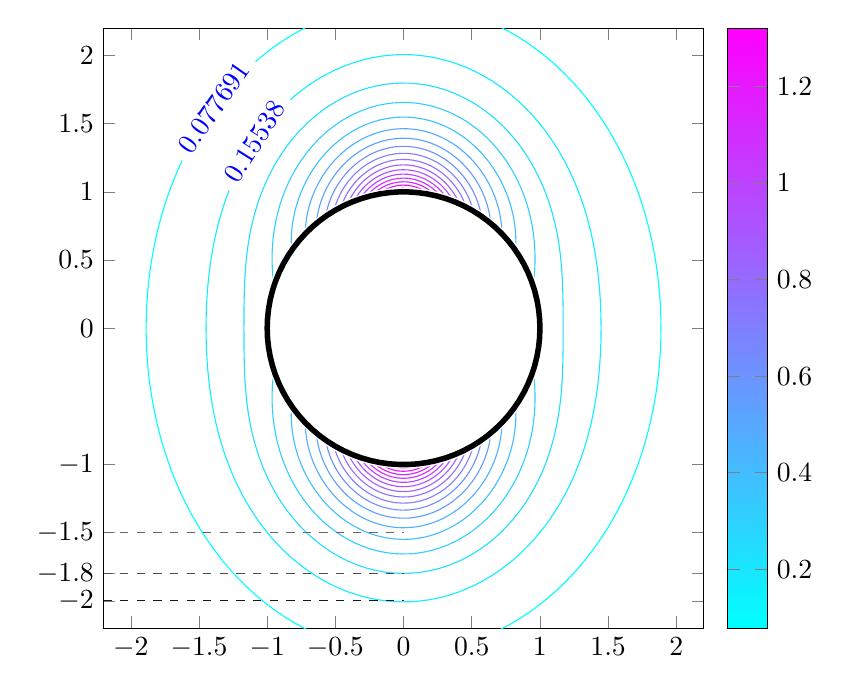
\begin{tikzpicture}

\begin{axis}[%
width=3in,
height=3in,
at={(0in,0in)},
scale only axis,
point meta min=0.0777,
point meta max=1.3207,
colormap={mymap}{[1pt] rgb(0pt)=(0,1,1); rgb(63pt)=(1,0,1)},
xmin=-2.2000,
xmax=2.2000,
ymin=-2.2000,
ymax=2.2000,
ytick={-2.0000,-1.8000,-1.5000,-1.0000,0.0000,0.5000,1.0000,1.5000,2.0000},
axis background/.style={fill=white},
colorbar
]
\addplot[contour prepared, contour prepared format=matlab, contour/labels=false] table[row sep=crcr] {%
%
0.0777	336.0000\\
1.8878	0.0000\\
1.8871	0.0663\\
1.8850	0.1326\\
1.8815	0.1989\\
1.8765	0.2652\\
1.8738	0.2940\\
1.8702	0.3316\\
1.8623	0.3981\\
1.8542	0.4560\\
1.8529	0.4647\\
1.8421	0.5313\\
1.8341	0.5742\\
1.8296	0.5980\\
1.8155	0.6648\\
1.8134	0.6738\\
1.7998	0.7317\\
1.7922	0.7606\\
1.7823	0.7985\\
1.7705	0.8397\\
1.7630	0.8654\\
1.7481	0.9129\\
1.7420	0.9323\\
1.7252	0.9812\\
1.7190	0.9992\\
1.7016	1.0457\\
1.6940	1.0659\\
1.6774	1.1070\\
1.6670	1.1325\\
1.6526	1.1657\\
1.6380	1.1989\\
1.6270	1.2221\\
1.6067	1.2649\\
1.6007	1.2768\\
1.5736	1.3299\\
1.5732	1.3306\\
1.5459	1.3806\\
1.5375	1.3958\\
1.5173	1.4302\\
1.4994	1.4604\\
1.4878	1.4788\\
1.4589	1.5243\\
1.4573	1.5266\\
1.4260	1.5726\\
1.4159	1.5874\\
1.3937	1.6178\\
1.3704	1.6494\\
1.3602	1.6625\\
1.3255	1.7064\\
1.3224	1.7103\\
1.2896	1.7490\\
1.2718	1.7699\\
1.2523	1.7912\\
1.2185	1.8280\\
1.2135	1.8331\\
1.1732	1.8739\\
1.1627	1.8844\\
1.1310	1.9141\\
1.1043	1.9389\\
1.0868	1.9540\\
1.0433	1.9912\\
1.0404	1.9935\\
0.9914	2.0322\\
0.9798	2.0412\\
0.9394	2.0704\\
0.9139	2.0887\\
0.8839	2.1083\\
0.8455	2.1333\\
0.8244	2.1458\\
0.7748	2.1749\\
0.7597	2.1829\\
0.7020	2.2133\\
0.6885	2.2196\\
0.6271	2.2482\\
0.6082	2.2559\\
0.5504	2.2794\\
0.5147	2.2918\\
0.4720	2.3067\\
0.4005	2.3275\\
0.3921	2.3299\\
0.3110	2.3490\\
0.2338	2.3628\\
0.2289	2.3636\\
0.1460	2.3739\\
0.0627	2.3796\\
-0.0209	2.3808\\
-0.1044	2.3773\\
-0.1875	2.3693\\
-0.2310	2.3627\\
-0.2700	2.3569\\
-0.3517	2.3400\\
-0.3994	2.3274\\
-0.4322	2.3188\\
-0.5114	2.2935\\
-0.5157	2.2919\\
-0.5890	2.2642\\
-0.6082	2.2559\\
-0.6648	2.2312\\
-0.6883	2.2195\\
-0.7387	2.1945\\
-0.7597	2.1829\\
-0.8104	2.1545\\
-0.8245	2.1458\\
-0.8800	2.1113\\
-0.8842	2.1085\\
-0.9395	2.0706\\
-0.9472	2.0653\\
-0.9914	2.0321\\
-1.0119	2.0165\\
-1.0404	1.9932\\
-1.0742	1.9653\\
-1.0868	1.9540\\
-1.1310	1.9144\\
-1.1338	1.9119\\
-1.1732	1.8738\\
-1.1910	1.8564\\
-1.2136	1.8328\\
-1.2455	1.7992\\
-1.2523	1.7915\\
-1.2896	1.7492\\
-1.2974	1.7403\\
-1.3255	1.7061\\
-1.3467	1.6801\\
-1.3602	1.6624\\
-1.3934	1.6185\\
-1.3935	1.6184\\
-1.4260	1.5726\\
-1.4377	1.5560\\
-1.4574	1.5261\\
-1.4794	1.4925\\
-1.4878	1.4789\\
-1.5172	1.4307\\
-1.5187	1.4282\\
-1.5459	1.3806\\
-1.5557	1.3633\\
-1.5737	1.3293\\
-1.5903	1.2978\\
-1.6007	1.2766\\
-1.6226	1.2319\\
-1.6269	1.2224\\
-1.6524	1.1663\\
-1.6527	1.1657\\
-1.6774	1.1073\\
-1.6808	1.0992\\
-1.7016	1.0458\\
-1.7067	1.0325\\
-1.7252	0.9813\\
-1.7307	0.9658\\
-1.7481	0.9130\\
-1.7527	0.8989\\
-1.7704	0.8402\\
-1.7729	0.8320\\
-1.7912	0.7651\\
-1.7922	0.7613\\
-1.8079	0.6982\\
-1.8134	0.6733\\
-1.8228	0.6314\\
-1.8341	0.5746\\
-1.8360	0.5647\\
-1.8477	0.4980\\
-1.8542	0.4554\\
-1.8578	0.4314\\
-1.8664	0.3649\\
-1.8735	0.2984\\
-1.8738	0.2956\\
-1.8792	0.2320\\
-1.8834	0.1657\\
-1.8862	0.0994\\
-1.8876	0.0331\\
-1.8876	-0.0331\\
-1.8862	-0.0994\\
-1.8834	-0.1657\\
-1.8792	-0.2320\\
-1.8738	-0.2956\\
-1.8735	-0.2984\\
-1.8664	-0.3649\\
-1.8578	-0.4314\\
-1.8542	-0.4554\\
-1.8477	-0.4980\\
-1.8360	-0.5647\\
-1.8341	-0.5746\\
-1.8228	-0.6314\\
-1.8134	-0.6733\\
-1.8079	-0.6982\\
-1.7922	-0.7613\\
-1.7912	-0.7651\\
-1.7729	-0.8320\\
-1.7704	-0.8402\\
-1.7527	-0.8989\\
-1.7481	-0.9130\\
-1.7307	-0.9658\\
-1.7252	-0.9813\\
-1.7067	-1.0325\\
-1.7016	-1.0458\\
-1.6808	-1.0992\\
-1.6774	-1.1073\\
-1.6527	-1.1657\\
-1.6524	-1.1663\\
-1.6269	-1.2224\\
-1.6226	-1.2319\\
-1.6007	-1.2766\\
-1.5903	-1.2978\\
-1.5737	-1.3293\\
-1.5557	-1.3633\\
-1.5459	-1.3806\\
-1.5187	-1.4282\\
-1.5172	-1.4307\\
-1.4878	-1.4789\\
-1.4794	-1.4925\\
-1.4574	-1.5261\\
-1.4377	-1.5560\\
-1.4260	-1.5726\\
-1.3935	-1.6184\\
-1.3934	-1.6185\\
-1.3602	-1.6624\\
-1.3467	-1.6801\\
-1.3255	-1.7061\\
-1.2974	-1.7403\\
-1.2896	-1.7492\\
-1.2523	-1.7915\\
-1.2455	-1.7992\\
-1.2136	-1.8328\\
-1.1910	-1.8564\\
-1.1732	-1.8738\\
-1.1338	-1.9119\\
-1.1310	-1.9144\\
-1.0868	-1.9540\\
-1.0742	-1.9653\\
-1.0404	-1.9932\\
-1.0119	-2.0165\\
-0.9914	-2.0321\\
-0.9472	-2.0653\\
-0.9395	-2.0706\\
-0.8842	-2.1085\\
-0.8800	-2.1113\\
-0.8245	-2.1458\\
-0.8104	-2.1545\\
-0.7597	-2.1829\\
-0.7387	-2.1945\\
-0.6883	-2.2195\\
-0.6648	-2.2312\\
-0.6082	-2.2559\\
-0.5890	-2.2642\\
-0.5157	-2.2919\\
-0.5114	-2.2935\\
-0.4322	-2.3188\\
-0.3994	-2.3274\\
-0.3517	-2.3400\\
-0.2700	-2.3569\\
-0.2310	-2.3627\\
-0.1875	-2.3693\\
-0.1044	-2.3773\\
-0.0209	-2.3808\\
0.0627	-2.3796\\
0.1460	-2.3739\\
0.2289	-2.3636\\
0.2338	-2.3628\\
0.3110	-2.3490\\
0.3921	-2.3299\\
0.4005	-2.3275\\
0.4720	-2.3067\\
0.5147	-2.2918\\
0.5504	-2.2794\\
0.6082	-2.2559\\
0.6271	-2.2482\\
0.6885	-2.2196\\
0.7020	-2.2133\\
0.7597	-2.1829\\
0.7748	-2.1749\\
0.8244	-2.1458\\
0.8455	-2.1333\\
0.8839	-2.1083\\
0.9139	-2.0887\\
0.9394	-2.0704\\
0.9798	-2.0412\\
0.9914	-2.0322\\
1.0404	-1.9935\\
1.0433	-1.9912\\
1.0868	-1.9540\\
1.1043	-1.9389\\
1.1310	-1.9141\\
1.1627	-1.8844\\
1.1732	-1.8739\\
1.2135	-1.8331\\
1.2185	-1.8280\\
1.2523	-1.7912\\
1.2718	-1.7699\\
1.2896	-1.7490\\
1.3224	-1.7103\\
1.3255	-1.7064\\
1.3602	-1.6625\\
1.3704	-1.6494\\
1.3937	-1.6178\\
1.4159	-1.5874\\
1.4260	-1.5726\\
1.4573	-1.5266\\
1.4589	-1.5243\\
1.4878	-1.4788\\
1.4994	-1.4604\\
1.5173	-1.4302\\
1.5375	-1.3958\\
1.5459	-1.3806\\
1.5732	-1.3306\\
1.5736	-1.3299\\
1.6007	-1.2768\\
1.6067	-1.2649\\
1.6270	-1.2221\\
1.6380	-1.1989\\
1.6526	-1.1657\\
1.6670	-1.1325\\
1.6774	-1.1070\\
1.6940	-1.0659\\
1.7016	-1.0457\\
1.7190	-0.9992\\
1.7252	-0.9812\\
1.7420	-0.9323\\
1.7481	-0.9129\\
1.7630	-0.8654\\
1.7705	-0.8397\\
1.7823	-0.7985\\
1.7922	-0.7606\\
1.7998	-0.7317\\
1.8134	-0.6738\\
1.8155	-0.6648\\
1.8296	-0.5980\\
1.8341	-0.5742\\
1.8421	-0.5313\\
1.8529	-0.4647\\
1.8542	-0.4560\\
1.8623	-0.3981\\
1.8702	-0.3316\\
1.8738	-0.2940\\
1.8765	-0.2652\\
1.8815	-0.1989\\
1.8850	-0.1326\\
1.8871	-0.0663\\
1.8878	-0.0000\\
0.0777	180.0000\\
0.9959	-0.0000\\
0.9953	-0.0349\\
0.9934	-0.0699\\
0.9903	-0.1047\\
0.9860	-0.1394\\
0.9805	-0.1739\\
0.9738	-0.2082\\
0.9658	-0.2422\\
0.9567	-0.2759\\
0.9463	-0.3093\\
0.9349	-0.3423\\
0.9222	-0.3749\\
0.9084	-0.4070\\
0.8935	-0.4386\\
0.8775	-0.4697\\
0.8604	-0.5001\\
0.8422	-0.5300\\
0.8231	-0.5591\\
0.8029	-0.5876\\
0.7817	-0.6154\\
0.7595	-0.6424\\
0.7364	-0.6686\\
0.7125	-0.6939\\
0.6876	-0.7184\\
0.6619	-0.7421\\
0.6354	-0.7648\\
0.6081	-0.7865\\
0.5801	-0.8073\\
0.5513	-0.8271\\
0.5219	-0.8458\\
0.4919	-0.8636\\
0.4612	-0.8802\\
0.4300	-0.8958\\
0.3983	-0.9103\\
0.3661	-0.9236\\
0.3334	-0.9359\\
0.3003	-0.9469\\
0.2669	-0.9568\\
0.2332	-0.9656\\
0.1991	-0.9731\\
0.1648	-0.9795\\
0.1304	-0.9846\\
0.0957	-0.9886\\
0.0610	-0.9913\\
0.0261	-0.9928\\
-0.0087	-0.9931\\
-0.0436	-0.9922\\
-0.0784	-0.9901\\
-0.1131	-0.9867\\
-0.1476	-0.9822\\
-0.1820	-0.9764\\
-0.2162	-0.9695\\
-0.2501	-0.9613\\
-0.2837	-0.9520\\
-0.3169	-0.9415\\
-0.3498	-0.9299\\
-0.3822	-0.9171\\
-0.4142	-0.9032\\
-0.4457	-0.8882\\
-0.4766	-0.8720\\
-0.5070	-0.8548\\
-0.5367	-0.8366\\
-0.5658	-0.8173\\
-0.5942	-0.7970\\
-0.6218	-0.7758\\
-0.6487	-0.7535\\
-0.6748	-0.7304\\
-0.7001	-0.7063\\
-0.7246	-0.6814\\
-0.7481	-0.6556\\
-0.7707	-0.6290\\
-0.7924	-0.6016\\
-0.8131	-0.5735\\
-0.8328	-0.5446\\
-0.8515	-0.5151\\
-0.8691	-0.4850\\
-0.8856	-0.4542\\
-0.9011	-0.4229\\
-0.9155	-0.3910\\
-0.9287	-0.3587\\
-0.9407	-0.3259\\
-0.9517	-0.2927\\
-0.9614	-0.2591\\
-0.9699	-0.2252\\
-0.9773	-0.1911\\
-0.9834	-0.1566\\
-0.9883	-0.1220\\
-0.9920	-0.0873\\
-0.9945	-0.0524\\
-0.9957	-0.0175\\
-0.9957	0.0175\\
-0.9945	0.0524\\
-0.9920	0.0873\\
-0.9883	0.1220\\
-0.9834	0.1566\\
-0.9773	0.1911\\
-0.9699	0.2252\\
-0.9614	0.2591\\
-0.9517	0.2927\\
-0.9407	0.3259\\
-0.9287	0.3587\\
-0.9155	0.3910\\
-0.9011	0.4229\\
-0.8856	0.4542\\
-0.8691	0.4850\\
-0.8515	0.5151\\
-0.8328	0.5446\\
-0.8131	0.5735\\
-0.7924	0.6016\\
-0.7707	0.6290\\
-0.7481	0.6556\\
-0.7246	0.6814\\
-0.7001	0.7063\\
-0.6748	0.7304\\
-0.6487	0.7535\\
-0.6218	0.7758\\
-0.5942	0.7970\\
-0.5658	0.8173\\
-0.5367	0.8366\\
-0.5070	0.8548\\
-0.4766	0.8720\\
-0.4457	0.8882\\
-0.4142	0.9032\\
-0.3822	0.9171\\
-0.3498	0.9299\\
-0.3169	0.9415\\
-0.2837	0.9520\\
-0.2501	0.9613\\
-0.2162	0.9695\\
-0.1820	0.9764\\
-0.1476	0.9822\\
-0.1131	0.9867\\
-0.0784	0.9901\\
-0.0436	0.9922\\
-0.0087	0.9931\\
0.0261	0.9928\\
0.0610	0.9913\\
0.0957	0.9886\\
0.1304	0.9846\\
0.1648	0.9795\\
0.1991	0.9731\\
0.2332	0.9656\\
0.2669	0.9568\\
0.3003	0.9469\\
0.3334	0.9359\\
0.3661	0.9236\\
0.3983	0.9103\\
0.4300	0.8958\\
0.4612	0.8802\\
0.4919	0.8636\\
0.5219	0.8458\\
0.5513	0.8271\\
0.5801	0.8073\\
0.6081	0.7865\\
0.6354	0.7648\\
0.6619	0.7421\\
0.6876	0.7184\\
0.7125	0.6939\\
0.7364	0.6686\\
0.7595	0.6424\\
0.7817	0.6154\\
0.8029	0.5876\\
0.8231	0.5591\\
0.8422	0.5300\\
0.8604	0.5001\\
0.8775	0.4697\\
0.8935	0.4386\\
0.9084	0.4070\\
0.9222	0.3749\\
0.9349	0.3423\\
0.9463	0.3093\\
0.9567	0.2759\\
0.9658	0.2422\\
0.9738	0.2082\\
0.9805	0.1739\\
0.9860	0.1394\\
0.9903	0.1047\\
0.9934	0.0699\\
0.9953	0.0349\\
0.9959	0.0000\\
0.1554	356.0000\\
1.4485	0.0000\\
1.4481	0.0509\\
1.4471	0.1018\\
1.4453	0.1528\\
1.4428	0.2039\\
1.4427	0.2054\\
1.4396	0.2553\\
1.4355	0.3069\\
1.4341	0.3212\\
1.4306	0.3588\\
1.4251	0.4082\\
1.4247	0.4109\\
1.4180	0.4635\\
1.4155	0.4802\\
1.4102	0.5164\\
1.4055	0.5446\\
1.4013	0.5697\\
1.3950	0.6034\\
1.3912	0.6233\\
1.3839	0.6582\\
1.3799	0.6773\\
1.3724	0.7097\\
1.3672	0.7317\\
1.3603	0.7586\\
1.3531	0.7865\\
1.3477	0.8056\\
1.3374	0.8415\\
1.3345	0.8511\\
1.3207	0.8951\\
1.3202	0.8968\\
1.3065	0.9371\\
1.3012	0.9524\\
1.2917	0.9783\\
1.2805	1.0081\\
1.2762	1.0188\\
1.2601	1.0585\\
1.2579	1.0638\\
1.2434	1.0968\\
1.2333	1.1196\\
1.2261	1.1348\\
1.2079	1.1725\\
1.2066	1.1752\\
1.1893	1.2088\\
1.1778	1.2306\\
1.1697	1.2451\\
1.1494	1.2810\\
1.1467	1.2856\\
1.1284	1.3158\\
1.1134	1.3401\\
1.1064	1.3508\\
1.0836	1.3852\\
1.0777	1.3939\\
1.0598	1.4190\\
1.0396	1.4468\\
1.0350	1.4529\\
1.0091	1.4860\\
0.9991	1.4988\\
0.9821	1.5189\\
0.9560	1.5494\\
0.9537	1.5519\\
0.9241	1.5841\\
0.9105	1.5986\\
0.8929	1.6162\\
0.8625	1.6461\\
0.8601	1.6483\\
0.8254	1.6798\\
0.8121	1.6917\\
0.7886	1.7111\\
0.7592	1.7352\\
0.7495	1.7424\\
0.7077	1.7735\\
0.7040	1.7762\\
0.6623	1.8041\\
0.6465	1.8147\\
0.6130	1.8347\\
0.5868	1.8502\\
0.5586	1.8651\\
0.5252	1.8826\\
0.4975	1.8953\\
0.4616	1.9117\\
0.4267	1.9253\\
0.3964	1.9372\\
0.3410	1.9552\\
0.3297	1.9589\\
0.2617	1.9768\\
0.2210	1.9849\\
0.1927	1.9906\\
0.1230	2.0002\\
0.0528	2.0056\\
-0.0176	2.0067\\
-0.0880	2.0034\\
-0.1580	1.9959\\
-0.2229	1.9849\\
-0.2273	1.9842\\
-0.2958	1.9684\\
-0.3405	1.9552\\
-0.3632	1.9485\\
-0.4276	1.9254\\
-0.4292	1.9249\\
-0.4936	1.8975\\
-0.4980	1.8954\\
-0.5562	1.8668\\
-0.5591	1.8652\\
-0.6133	1.8348\\
-0.6169	1.8328\\
-0.6623	1.8042\\
-0.6755	1.7958\\
-0.7075	1.7733\\
-0.7319	1.7560\\
-0.7495	1.7424\\
-0.7859	1.7137\\
-0.7887	1.7114\\
-0.8254	1.6798\\
-0.8376	1.6692\\
-0.8601	1.6481\\
-0.8868	1.6226\\
-0.8929	1.6164\\
-0.9241	1.5842\\
-0.9336	1.5742\\
-0.9538	1.5516\\
-0.9779	1.5242\\
-0.9820	1.5192\\
-1.0091	1.4860\\
-1.0196	1.4730\\
-1.0350	1.4526\\
-1.0589	1.4205\\
-1.0597	1.4194\\
-1.0836	1.3850\\
-1.0958	1.3671\\
-1.1064	1.3507\\
-1.1283	1.3162\\
-1.1303	1.3129\\
-1.1495	1.2806\\
-1.1625	1.2582\\
-1.1697	1.2451\\
-1.1892	1.2091\\
-1.1924	1.2029\\
-1.2080	1.1721\\
-1.2202	1.1474\\
-1.2260	1.1349\\
-1.2434	1.0971\\
-1.2458	1.0917\\
-1.2602	1.0581\\
-1.2694	1.0360\\
-1.2762	1.0187\\
-1.2911	0.9802\\
-1.2916	0.9788\\
-1.3065	0.9371\\
-1.3109	0.9246\\
-1.3208	0.8945\\
-1.3290	0.8692\\
-1.3345	0.8509\\
-1.3454	0.8140\\
-1.3476	0.8059\\
-1.3602	0.7593\\
-1.3603	0.7590\\
-1.3723	0.7101\\
-1.3737	0.7045\\
-1.3839	0.6584\\
-1.3857	0.6503\\
-1.3949	0.6038\\
-1.3964	0.5964\\
-1.4055	0.5452\\
-1.4059	0.5430\\
-1.4142	0.4899\\
-1.4155	0.4805\\
-1.4215	0.4372\\
-1.4251	0.4075\\
-1.4278	0.3848\\
-1.4331	0.3328\\
-1.4341	0.3213\\
-1.4376	0.2810\\
-1.4413	0.2296\\
-1.4427	0.2039\\
-1.4442	0.1783\\
-1.4463	0.1272\\
-1.4477	0.0763\\
-1.4484	0.0254\\
-1.4484	-0.0254\\
-1.4477	-0.0763\\
-1.4463	-0.1272\\
-1.4442	-0.1783\\
-1.4427	-0.2039\\
-1.4413	-0.2296\\
-1.4376	-0.2810\\
-1.4341	-0.3213\\
-1.4331	-0.3328\\
-1.4278	-0.3848\\
-1.4251	-0.4075\\
-1.4215	-0.4372\\
-1.4155	-0.4805\\
-1.4142	-0.4899\\
-1.4059	-0.5430\\
-1.4055	-0.5452\\
-1.3964	-0.5964\\
-1.3949	-0.6038\\
-1.3857	-0.6503\\
-1.3839	-0.6584\\
-1.3737	-0.7045\\
-1.3723	-0.7101\\
-1.3603	-0.7590\\
-1.3602	-0.7593\\
-1.3476	-0.8059\\
-1.3454	-0.8140\\
-1.3345	-0.8509\\
-1.3290	-0.8692\\
-1.3208	-0.8945\\
-1.3109	-0.9246\\
-1.3065	-0.9371\\
-1.2916	-0.9788\\
-1.2911	-0.9802\\
-1.2762	-1.0187\\
-1.2694	-1.0360\\
-1.2602	-1.0581\\
-1.2458	-1.0917\\
-1.2434	-1.0971\\
-1.2260	-1.1349\\
-1.2202	-1.1474\\
-1.2080	-1.1721\\
-1.1924	-1.2029\\
-1.1892	-1.2091\\
-1.1697	-1.2451\\
-1.1625	-1.2582\\
-1.1495	-1.2806\\
-1.1303	-1.3129\\
-1.1283	-1.3162\\
-1.1064	-1.3507\\
-1.0958	-1.3671\\
-1.0836	-1.3850\\
-1.0597	-1.4194\\
-1.0589	-1.4205\\
-1.0350	-1.4526\\
-1.0196	-1.4730\\
-1.0091	-1.4860\\
-0.9820	-1.5192\\
-0.9779	-1.5242\\
-0.9538	-1.5516\\
-0.9336	-1.5742\\
-0.9241	-1.5842\\
-0.8929	-1.6164\\
-0.8868	-1.6226\\
-0.8601	-1.6481\\
-0.8376	-1.6692\\
-0.8254	-1.6798\\
-0.7887	-1.7114\\
-0.7859	-1.7137\\
-0.7495	-1.7424\\
-0.7319	-1.7560\\
-0.7075	-1.7733\\
-0.6755	-1.7958\\
-0.6623	-1.8042\\
-0.6169	-1.8328\\
-0.6133	-1.8348\\
-0.5591	-1.8652\\
-0.5562	-1.8668\\
-0.4980	-1.8954\\
-0.4936	-1.8975\\
-0.4292	-1.9249\\
-0.4276	-1.9254\\
-0.3632	-1.9485\\
-0.3405	-1.9552\\
-0.2958	-1.9684\\
-0.2273	-1.9842\\
-0.2229	-1.9849\\
-0.1580	-1.9959\\
-0.0880	-2.0034\\
-0.0176	-2.0067\\
0.0528	-2.0056\\
0.1230	-2.0002\\
0.1927	-1.9906\\
0.2210	-1.9849\\
0.2617	-1.9768\\
0.3297	-1.9589\\
0.3410	-1.9552\\
0.3964	-1.9372\\
0.4267	-1.9253\\
0.4616	-1.9117\\
0.4975	-1.8953\\
0.5252	-1.8826\\
0.5586	-1.8651\\
0.5868	-1.8502\\
0.6130	-1.8347\\
0.6465	-1.8147\\
0.6623	-1.8041\\
0.7040	-1.7762\\
0.7077	-1.7735\\
0.7495	-1.7424\\
0.7592	-1.7352\\
0.7886	-1.7111\\
0.8121	-1.6917\\
0.8254	-1.6798\\
0.8601	-1.6483\\
0.8625	-1.6461\\
0.8929	-1.6162\\
0.9105	-1.5986\\
0.9241	-1.5841\\
0.9537	-1.5519\\
0.9560	-1.5494\\
0.9821	-1.5189\\
0.9991	-1.4988\\
1.0091	-1.4860\\
1.0350	-1.4529\\
1.0396	-1.4468\\
1.0598	-1.4190\\
1.0777	-1.3939\\
1.0836	-1.3852\\
1.1064	-1.3508\\
1.1134	-1.3401\\
1.1284	-1.3158\\
1.1467	-1.2856\\
1.1494	-1.2810\\
1.1697	-1.2451\\
1.1778	-1.2306\\
1.1893	-1.2088\\
1.2066	-1.1752\\
1.2079	-1.1725\\
1.2261	-1.1348\\
1.2333	-1.1196\\
1.2434	-1.0968\\
1.2579	-1.0638\\
1.2601	-1.0585\\
1.2762	-1.0188\\
1.2805	-1.0081\\
1.2917	-0.9783\\
1.3012	-0.9524\\
1.3065	-0.9371\\
1.3202	-0.8968\\
1.3207	-0.8951\\
1.3345	-0.8511\\
1.3374	-0.8415\\
1.3477	-0.8056\\
1.3531	-0.7865\\
1.3603	-0.7586\\
1.3672	-0.7317\\
1.3724	-0.7097\\
1.3799	-0.6773\\
1.3839	-0.6582\\
1.3912	-0.6233\\
1.3950	-0.6034\\
1.4013	-0.5697\\
1.4055	-0.5446\\
1.4102	-0.5164\\
1.4155	-0.4802\\
1.4180	-0.4635\\
1.4247	-0.4109\\
1.4251	-0.4082\\
1.4306	-0.3588\\
1.4341	-0.3212\\
1.4355	-0.3069\\
1.4396	-0.2553\\
1.4427	-0.2054\\
1.4428	-0.2039\\
1.4453	-0.1528\\
1.4471	-0.1018\\
1.4481	-0.0509\\
1.4485	-0.0000\\
0.1554	180.0000\\
0.9993	-0.0000\\
0.9987	-0.0351\\
0.9968	-0.0701\\
0.9937	-0.1050\\
0.9894	-0.1398\\
0.9838	-0.1745\\
0.9770	-0.2089\\
0.9690	-0.2430\\
0.9598	-0.2768\\
0.9493	-0.3103\\
0.9378	-0.3434\\
0.9250	-0.3760\\
0.9111	-0.4082\\
0.8961	-0.4399\\
0.8800	-0.4710\\
0.8628	-0.5015\\
0.8445	-0.5314\\
0.8252	-0.5606\\
0.8048	-0.5891\\
0.7835	-0.6169\\
0.7613	-0.6439\\
0.7381	-0.6700\\
0.7140	-0.6954\\
0.6890	-0.7199\\
0.6632	-0.7435\\
0.6365	-0.7662\\
0.6091	-0.7879\\
0.5810	-0.8086\\
0.5522	-0.8284\\
0.5227	-0.8471\\
0.4925	-0.8648\\
0.4618	-0.8814\\
0.4305	-0.8969\\
0.3987	-0.9113\\
0.3665	-0.9246\\
0.3337	-0.9368\\
0.3006	-0.9478\\
0.2671	-0.9577\\
0.2334	-0.9664\\
0.1993	-0.9739\\
0.1650	-0.9802\\
0.1305	-0.9854\\
0.0958	-0.9893\\
0.0610	-0.9920\\
0.0262	-0.9935\\
-0.0087	-0.9938\\
-0.0436	-0.9929\\
-0.0784	-0.9908\\
-0.1131	-0.9875\\
-0.1477	-0.9829\\
-0.1822	-0.9772\\
-0.2163	-0.9703\\
-0.2503	-0.9622\\
-0.2839	-0.9529\\
-0.3172	-0.9425\\
-0.3502	-0.9309\\
-0.3827	-0.9181\\
-0.4147	-0.9042\\
-0.4462	-0.8893\\
-0.4773	-0.8732\\
-0.5077	-0.8561\\
-0.5375	-0.8378\\
-0.5667	-0.8186\\
-0.5952	-0.7984\\
-0.6229	-0.7771\\
-0.6499	-0.7549\\
-0.6762	-0.7318\\
-0.7016	-0.7078\\
-0.7261	-0.6828\\
-0.7498	-0.6570\\
-0.7725	-0.6305\\
-0.7943	-0.6031\\
-0.8151	-0.5749\\
-0.8350	-0.5461\\
-0.8538	-0.5165\\
-0.8715	-0.4863\\
-0.8882	-0.4555\\
-0.9037	-0.4241\\
-0.9182	-0.3922\\
-0.9315	-0.3598\\
-0.9437	-0.3269\\
-0.9547	-0.2936\\
-0.9645	-0.2600\\
-0.9731	-0.2260\\
-0.9805	-0.1917\\
-0.9867	-0.1572\\
-0.9917	-0.1225\\
-0.9954	-0.0876\\
-0.9979	-0.0526\\
-0.9991	-0.0175\\
-0.9991	0.0175\\
-0.9979	0.0526\\
-0.9954	0.0876\\
-0.9917	0.1225\\
-0.9867	0.1572\\
-0.9805	0.1917\\
-0.9731	0.2260\\
-0.9645	0.2600\\
-0.9547	0.2936\\
-0.9437	0.3269\\
-0.9315	0.3598\\
-0.9182	0.3922\\
-0.9037	0.4241\\
-0.8882	0.4555\\
-0.8715	0.4863\\
-0.8538	0.5165\\
-0.8350	0.5461\\
-0.8151	0.5749\\
-0.7943	0.6031\\
-0.7725	0.6305\\
-0.7498	0.6570\\
-0.7261	0.6828\\
-0.7016	0.7078\\
-0.6762	0.7318\\
-0.6499	0.7549\\
-0.6229	0.7771\\
-0.5952	0.7984\\
-0.5667	0.8186\\
-0.5375	0.8378\\
-0.5077	0.8561\\
-0.4773	0.8732\\
-0.4462	0.8893\\
-0.4147	0.9042\\
-0.3827	0.9181\\
-0.3502	0.9309\\
-0.3172	0.9425\\
-0.2839	0.9529\\
-0.2503	0.9622\\
-0.2163	0.9703\\
-0.1822	0.9772\\
-0.1477	0.9829\\
-0.1131	0.9875\\
-0.0784	0.9908\\
-0.0436	0.9929\\
-0.0087	0.9938\\
0.0262	0.9935\\
0.0610	0.9920\\
0.0958	0.9893\\
0.1305	0.9854\\
0.1650	0.9802\\
0.1993	0.9739\\
0.2334	0.9664\\
0.2671	0.9577\\
0.3006	0.9478\\
0.3337	0.9368\\
0.3665	0.9246\\
0.3987	0.9113\\
0.4305	0.8969\\
0.4618	0.8814\\
0.4925	0.8648\\
0.5227	0.8471\\
0.5522	0.8284\\
0.5810	0.8086\\
0.6091	0.7879\\
0.6365	0.7662\\
0.6632	0.7435\\
0.6890	0.7199\\
0.7140	0.6954\\
0.7381	0.6700\\
0.7613	0.6439\\
0.7835	0.6169\\
0.8048	0.5891\\
0.8252	0.5606\\
0.8445	0.5314\\
0.8628	0.5015\\
0.8800	0.4710\\
0.8961	0.4399\\
0.9111	0.4082\\
0.9250	0.3760\\
0.9378	0.3434\\
0.9493	0.3103\\
0.9598	0.2768\\
0.9690	0.2430\\
0.9770	0.2089\\
0.9838	0.1745\\
0.9894	0.1398\\
0.9937	0.1050\\
0.9968	0.0701\\
0.9987	0.0351\\
0.9993	0.0000\\
0.2331	380.0000\\
1.1705	0.0000\\
1.1704	0.0411\\
1.1703	0.0823\\
1.1700	0.1237\\
1.1697	0.1622\\
1.1696	0.1653\\
1.1690	0.2073\\
1.1683	0.2435\\
1.1681	0.2497\\
1.1669	0.2926\\
1.1664	0.3060\\
1.1652	0.3361\\
1.1641	0.3598\\
1.1630	0.3801\\
1.1612	0.4084\\
1.1601	0.4248\\
1.1579	0.4534\\
1.1565	0.4702\\
1.1542	0.4957\\
1.1521	0.5162\\
1.1499	0.5359\\
1.1467	0.5629\\
1.1451	0.5747\\
1.1402	0.6102\\
1.1398	0.6124\\
1.1341	0.6484\\
1.1325	0.6583\\
1.1279	0.6836\\
1.1234	0.7069\\
1.1211	0.7184\\
1.1138	0.7525\\
1.1130	0.7561\\
1.1061	0.7854\\
1.1010	0.8058\\
1.0977	0.8183\\
1.0888	0.8509\\
1.0873	0.8560\\
1.0795	0.8824\\
1.0719	0.9066\\
1.0694	0.9142\\
1.0589	0.9453\\
1.0546	0.9574\\
1.0478	0.9760\\
1.0359	1.0070\\
1.0353	1.0084\\
1.0237	1.0369\\
1.0140	1.0595\\
1.0106	1.0672\\
0.9969	1.0969\\
0.9905	1.1105\\
0.9826	1.1264\\
0.9674	1.1561\\
0.9648	1.1612\\
0.9517	1.1850\\
0.9367	1.2115\\
0.9350	1.2144\\
0.9177	1.2430\\
0.9063	1.2613\\
0.8993	1.2718\\
0.8801	1.3003\\
0.8734	1.3102\\
0.8600	1.3287\\
0.8387	1.3573\\
0.8380	1.3581\\
0.8164	1.3851\\
0.8002	1.4049\\
0.7929	1.4132\\
0.7680	1.4411\\
0.7599	1.4502\\
0.7418	1.4688\\
0.7170	1.4937\\
0.7139	1.4967\\
0.6843	1.5241\\
0.6718	1.5354\\
0.6526	1.5515\\
0.6242	1.5749\\
0.6186	1.5790\\
0.5819	1.6062\\
0.5742	1.6119\\
0.5418	1.6333\\
0.5221	1.6462\\
0.4977	1.6604\\
0.4680	1.6776\\
0.4484	1.6874\\
0.4119	1.7057\\
0.3919	1.7143\\
0.3541	1.7305\\
0.3243	1.7411\\
0.2948	1.7517\\
0.2380	1.7679\\
0.2342	1.7690\\
0.1726	1.7825\\
0.1102	1.7918\\
0.0774	1.7945\\
0.0473	1.7971\\
-0.0158	1.7981\\
-0.0788	1.7949\\
-0.0822	1.7945\\
-0.1415	1.7877\\
-0.2035	1.7762\\
-0.2367	1.7679\\
-0.2646	1.7608\\
-0.3246	1.7415\\
-0.3254	1.7412\\
-0.3832	1.7185\\
-0.3923	1.7143\\
-0.4401	1.6920\\
-0.4487	1.6875\\
-0.4953	1.6622\\
-0.4981	1.6605\\
-0.5420	1.6334\\
-0.5485	1.6294\\
-0.5818	1.6062\\
-0.5995	1.5937\\
-0.6186	1.5789\\
-0.6483	1.5554\\
-0.6526	1.5517\\
-0.6843	1.5241\\
-0.6947	1.5148\\
-0.7139	1.4965\\
-0.7388	1.4722\\
-0.7418	1.4690\\
-0.7681	1.4411\\
-0.7803	1.4277\\
-0.7929	1.4131\\
-0.8164	1.3853\\
-0.8194	1.3817\\
-0.8388	1.3569\\
-0.8560	1.3343\\
-0.8599	1.3289\\
-0.8801	1.3003\\
-0.8901	1.2858\\
-0.8994	1.2717\\
-0.9176	1.2431\\
-0.9218	1.2365\\
-0.9351	1.2141\\
-0.9510	1.1864\\
-0.9516	1.1854\\
-0.9675	1.1558\\
-0.9779	1.1359\\
-0.9826	1.1266\\
-0.9969	1.0969\\
-1.0025	1.0850\\
-1.0106	1.0670\\
-1.0236	1.0372\\
-1.0249	1.0340\\
-1.0360	1.0066\\
-1.0452	0.9829\\
-1.0477	0.9763\\
-1.0589	0.9453\\
-1.0635	0.9320\\
-1.0695	0.9140\\
-1.0793	0.8829\\
-1.0798	0.8813\\
-1.0889	0.8506\\
-1.0944	0.8309\\
-1.0977	0.8184\\
-1.1060	0.7858\\
-1.1072	0.7809\\
-1.1139	0.7521\\
-1.1184	0.7314\\
-1.1211	0.7183\\
-1.1278	0.6841\\
-1.1281	0.6825\\
-1.1341	0.6483\\
-1.1365	0.6342\\
-1.1399	0.6120\\
-1.1436	0.5865\\
-1.1451	0.5747\\
-1.1495	0.5394\\
-1.1498	0.5364\\
-1.1541	0.4961\\
-1.1544	0.4931\\
-1.1579	0.4537\\
-1.1584	0.4474\\
-1.1612	0.4087\\
-1.1616	0.4024\\
-1.1640	0.3604\\
-1.1642	0.3580\\
-1.1661	0.3143\\
-1.1664	0.3062\\
-1.1676	0.2711\\
-1.1683	0.2431\\
-1.1686	0.2285\\
-1.1694	0.1863\\
-1.1697	0.1613\\
-1.1699	0.1445\\
-1.1702	0.1030\\
-1.1704	0.0617\\
-1.1705	0.0205\\
-1.1705	-0.0205\\
-1.1704	-0.0617\\
-1.1702	-0.1030\\
-1.1699	-0.1445\\
-1.1697	-0.1613\\
-1.1694	-0.1863\\
-1.1686	-0.2285\\
-1.1683	-0.2431\\
-1.1676	-0.2711\\
-1.1664	-0.3062\\
-1.1661	-0.3143\\
-1.1642	-0.3580\\
-1.1640	-0.3604\\
-1.1616	-0.4024\\
-1.1612	-0.4087\\
-1.1584	-0.4474\\
-1.1579	-0.4537\\
-1.1544	-0.4931\\
-1.1541	-0.4961\\
-1.1498	-0.5364\\
-1.1495	-0.5394\\
-1.1451	-0.5747\\
-1.1436	-0.5865\\
-1.1399	-0.6120\\
-1.1365	-0.6342\\
-1.1341	-0.6483\\
-1.1281	-0.6825\\
-1.1278	-0.6841\\
-1.1211	-0.7183\\
-1.1184	-0.7314\\
-1.1139	-0.7521\\
-1.1072	-0.7809\\
-1.1060	-0.7858\\
-1.0977	-0.8184\\
-1.0944	-0.8309\\
-1.0889	-0.8506\\
-1.0798	-0.8813\\
-1.0793	-0.8829\\
-1.0695	-0.9140\\
-1.0635	-0.9320\\
-1.0589	-0.9453\\
-1.0477	-0.9763\\
-1.0452	-0.9829\\
-1.0360	-1.0066\\
-1.0249	-1.0340\\
-1.0236	-1.0372\\
-1.0106	-1.0670\\
-1.0025	-1.0850\\
-0.9969	-1.0969\\
-0.9826	-1.1266\\
-0.9779	-1.1359\\
-0.9675	-1.1558\\
-0.9516	-1.1854\\
-0.9510	-1.1864\\
-0.9351	-1.2141\\
-0.9218	-1.2365\\
-0.9176	-1.2431\\
-0.8994	-1.2717\\
-0.8901	-1.2858\\
-0.8801	-1.3003\\
-0.8599	-1.3289\\
-0.8560	-1.3343\\
-0.8388	-1.3569\\
-0.8194	-1.3817\\
-0.8164	-1.3853\\
-0.7929	-1.4131\\
-0.7803	-1.4277\\
-0.7681	-1.4411\\
-0.7418	-1.4690\\
-0.7388	-1.4722\\
-0.7139	-1.4965\\
-0.6947	-1.5148\\
-0.6843	-1.5241\\
-0.6526	-1.5517\\
-0.6483	-1.5554\\
-0.6186	-1.5789\\
-0.5995	-1.5937\\
-0.5818	-1.6062\\
-0.5485	-1.6294\\
-0.5420	-1.6334\\
-0.4981	-1.6605\\
-0.4953	-1.6622\\
-0.4487	-1.6875\\
-0.4401	-1.6920\\
-0.3923	-1.7143\\
-0.3832	-1.7185\\
-0.3254	-1.7412\\
-0.3246	-1.7415\\
-0.2646	-1.7608\\
-0.2367	-1.7679\\
-0.2035	-1.7762\\
-0.1415	-1.7877\\
-0.0822	-1.7945\\
-0.0788	-1.7949\\
-0.0158	-1.7981\\
0.0473	-1.7971\\
0.0774	-1.7945\\
0.1102	-1.7918\\
0.1726	-1.7825\\
0.2342	-1.7690\\
0.2380	-1.7679\\
0.2948	-1.7517\\
0.3243	-1.7411\\
0.3541	-1.7305\\
0.3919	-1.7143\\
0.4119	-1.7057\\
0.4484	-1.6874\\
0.4680	-1.6776\\
0.4977	-1.6604\\
0.5221	-1.6462\\
0.5418	-1.6333\\
0.5742	-1.6119\\
0.5819	-1.6062\\
0.6186	-1.5790\\
0.6242	-1.5749\\
0.6526	-1.5515\\
0.6718	-1.5354\\
0.6843	-1.5241\\
0.7139	-1.4967\\
0.7170	-1.4937\\
0.7418	-1.4688\\
0.7599	-1.4502\\
0.7680	-1.4411\\
0.7929	-1.4132\\
0.8002	-1.4049\\
0.8164	-1.3851\\
0.8380	-1.3581\\
0.8387	-1.3573\\
0.8600	-1.3287\\
0.8734	-1.3102\\
0.8801	-1.3003\\
0.8993	-1.2718\\
0.9063	-1.2613\\
0.9177	-1.2430\\
0.9350	-1.2144\\
0.9367	-1.2115\\
0.9517	-1.1850\\
0.9648	-1.1612\\
0.9674	-1.1561\\
0.9826	-1.1264\\
0.9905	-1.1105\\
0.9969	-1.0969\\
1.0106	-1.0672\\
1.0140	-1.0595\\
1.0237	-1.0369\\
1.0353	-1.0084\\
1.0359	-1.0070\\
1.0478	-0.9760\\
1.0546	-0.9574\\
1.0589	-0.9453\\
1.0694	-0.9142\\
1.0719	-0.9066\\
1.0795	-0.8824\\
1.0873	-0.8560\\
1.0888	-0.8509\\
1.0977	-0.8183\\
1.1010	-0.8058\\
1.1061	-0.7854\\
1.1130	-0.7561\\
1.1138	-0.7525\\
1.1211	-0.7184\\
1.1234	-0.7069\\
1.1279	-0.6836\\
1.1325	-0.6583\\
1.1341	-0.6484\\
1.1398	-0.6124\\
1.1402	-0.6102\\
1.1451	-0.5747\\
1.1467	-0.5629\\
1.1499	-0.5359\\
1.1521	-0.5162\\
1.1542	-0.4957\\
1.1565	-0.4702\\
1.1579	-0.4534\\
1.1601	-0.4248\\
1.1612	-0.4084\\
1.1630	-0.3801\\
1.1641	-0.3598\\
1.1652	-0.3361\\
1.1664	-0.3060\\
1.1669	-0.2926\\
1.1681	-0.2497\\
1.1683	-0.2435\\
1.1690	-0.2073\\
1.1696	-0.1653\\
1.1697	-0.1622\\
1.1700	-0.1237\\
1.1703	-0.0823\\
1.1704	-0.0411\\
1.1705	-0.0000\\
0.2331	180.0000\\
1.0027	-0.0000\\
1.0021	-0.0352\\
1.0002	-0.0703\\
0.9971	-0.1054\\
0.9927	-0.1403\\
0.9871	-0.1750\\
0.9802	-0.2095\\
0.9721	-0.2438\\
0.9628	-0.2777\\
0.9523	-0.3113\\
0.9407	-0.3445\\
0.9278	-0.3772\\
0.9138	-0.4094\\
0.8987	-0.4411\\
0.8825	-0.4723\\
0.8651	-0.5029\\
0.8467	-0.5328\\
0.8273	-0.5620\\
0.8068	-0.5905\\
0.7854	-0.6183\\
0.7630	-0.6453\\
0.7397	-0.6715\\
0.7155	-0.6969\\
0.6904	-0.7213\\
0.6644	-0.7449\\
0.6377	-0.7675\\
0.6102	-0.7892\\
0.5820	-0.8099\\
0.5530	-0.8296\\
0.5234	-0.8483\\
0.4932	-0.8659\\
0.4624	-0.8825\\
0.4311	-0.8980\\
0.3992	-0.9124\\
0.3669	-0.9256\\
0.3341	-0.9377\\
0.3009	-0.9487\\
0.2674	-0.9585\\
0.2336	-0.9672\\
0.1994	-0.9747\\
0.1651	-0.9810\\
0.1306	-0.9861\\
0.0959	-0.9900\\
0.0611	-0.9927\\
0.0262	-0.9942\\
-0.0087	-0.9945\\
-0.0436	-0.9936\\
-0.0785	-0.9915\\
-0.1132	-0.9882\\
-0.1478	-0.9837\\
-0.1823	-0.9780\\
-0.2165	-0.9711\\
-0.2505	-0.9630\\
-0.2842	-0.9538\\
-0.3175	-0.9434\\
-0.3505	-0.9318\\
-0.3831	-0.9191\\
-0.4152	-0.9053\\
-0.4468	-0.8904\\
-0.4779	-0.8744\\
-0.5084	-0.8573\\
-0.5383	-0.8391\\
-0.5676	-0.8199\\
-0.5962	-0.7997\\
-0.6240	-0.7785\\
-0.6512	-0.7563\\
-0.6775	-0.7332\\
-0.7030	-0.7092\\
-0.7277	-0.6843\\
-0.7515	-0.6585\\
-0.7743	-0.6319\\
-0.7962	-0.6045\\
-0.8172	-0.5764\\
-0.8371	-0.5475\\
-0.8561	-0.5179\\
-0.8739	-0.4877\\
-0.8907	-0.4568\\
-0.9064	-0.4254\\
-0.9210	-0.3934\\
-0.9344	-0.3609\\
-0.9467	-0.3279\\
-0.9577	-0.2945\\
-0.9676	-0.2608\\
-0.9763	-0.2267\\
-0.9838	-0.1923\\
-0.9900	-0.1577\\
-0.9950	-0.1229\\
-0.9988	-0.0879\\
-1.0013	-0.0528\\
-1.0026	-0.0176\\
-1.0026	0.0176\\
-1.0013	0.0528\\
-0.9988	0.0879\\
-0.9950	0.1229\\
-0.9900	0.1577\\
-0.9838	0.1923\\
-0.9763	0.2267\\
-0.9676	0.2608\\
-0.9577	0.2945\\
-0.9467	0.3279\\
-0.9344	0.3609\\
-0.9210	0.3934\\
-0.9064	0.4254\\
-0.8907	0.4568\\
-0.8739	0.4877\\
-0.8561	0.5179\\
-0.8371	0.5475\\
-0.8172	0.5764\\
-0.7962	0.6045\\
-0.7743	0.6319\\
-0.7515	0.6585\\
-0.7277	0.6843\\
-0.7030	0.7092\\
-0.6775	0.7332\\
-0.6512	0.7563\\
-0.6240	0.7785\\
-0.5962	0.7997\\
-0.5676	0.8199\\
-0.5383	0.8391\\
-0.5084	0.8573\\
-0.4779	0.8744\\
-0.4468	0.8904\\
-0.4152	0.9053\\
-0.3831	0.9191\\
-0.3505	0.9318\\
-0.3175	0.9434\\
-0.2842	0.9538\\
-0.2505	0.9630\\
-0.2165	0.9711\\
-0.1823	0.9780\\
-0.1478	0.9837\\
-0.1132	0.9882\\
-0.0785	0.9915\\
-0.0436	0.9936\\
-0.0087	0.9945\\
0.0262	0.9942\\
0.0611	0.9927\\
0.0959	0.9900\\
0.1306	0.9861\\
0.1651	0.9810\\
0.1994	0.9747\\
0.2336	0.9672\\
0.2674	0.9585\\
0.3009	0.9487\\
0.3341	0.9377\\
0.3669	0.9256\\
0.3992	0.9124\\
0.4311	0.8980\\
0.4624	0.8825\\
0.4932	0.8659\\
0.5234	0.8483\\
0.5530	0.8296\\
0.5820	0.8099\\
0.6102	0.7892\\
0.6377	0.7675\\
0.6644	0.7449\\
0.6904	0.7213\\
0.7155	0.6969\\
0.7397	0.6715\\
0.7630	0.6453\\
0.7854	0.6183\\
0.8068	0.5905\\
0.8273	0.5620\\
0.8467	0.5328\\
0.8651	0.5029\\
0.8825	0.4723\\
0.8987	0.4411\\
0.9138	0.4094\\
0.9278	0.3772\\
0.9407	0.3445\\
0.9523	0.3113\\
0.9628	0.2777\\
0.9721	0.2438\\
0.9802	0.2095\\
0.9871	0.1750\\
0.9927	0.1403\\
0.9971	0.1054\\
1.0002	0.0703\\
1.0021	0.0352\\
1.0027	0.0000\\
0.3108	247.0000\\
0.9436	0.3455\\
0.9527	0.3198\\
0.9558	0.3493\\
0.9558	0.3500\\
0.9584	0.3773\\
0.9593	0.3900\\
0.9605	0.4053\\
0.9620	0.4310\\
0.9621	0.4334\\
0.9633	0.4604\\
0.9636	0.4730\\
0.9640	0.4875\\
0.9641	0.5149\\
0.9641	0.5160\\
0.9638	0.5412\\
0.9632	0.5599\\
0.9630	0.5680\\
0.9616	0.5944\\
0.9610	0.6046\\
0.9598	0.6207\\
0.9574	0.6473\\
0.9572	0.6502\\
0.9547	0.6731\\
0.9517	0.6966\\
0.9513	0.6996\\
0.9476	0.7253\\
0.9445	0.7436\\
0.9432	0.7515\\
0.9383	0.7773\\
0.9355	0.7912\\
0.9329	0.8032\\
0.9269	0.8290\\
0.9244	0.8392\\
0.9205	0.8547\\
0.9134	0.8806\\
0.9113	0.8877\\
0.9058	0.9061\\
0.8975	0.9320\\
0.8961	0.9363\\
0.8889	0.9573\\
0.8793	0.9832\\
0.8786	0.9850\\
0.8694	1.0084\\
0.8588	1.0337\\
0.8586	1.0343\\
0.8474	1.0593\\
0.8367	1.0821\\
0.8352	1.0851\\
0.8226	1.1102\\
0.8120	1.1301\\
0.8089	1.1357\\
0.7947	1.1609\\
0.7849	1.1775\\
0.7795	1.1863\\
0.7635	1.2115\\
0.7553	1.2240\\
0.7465	1.2367\\
0.7285	1.2620\\
0.7231	1.2695\\
0.7095	1.2870\\
0.6893	1.3124\\
0.6883	1.3136\\
0.6679	1.3372\\
0.6510	1.3562\\
0.6450	1.3624\\
0.6207	1.3874\\
0.6112	1.3970\\
0.5946	1.4124\\
0.5690	1.4356\\
0.5667	1.4375\\
0.5364	1.4623\\
0.5244	1.4720\\
0.5034	1.4872\\
0.4776	1.5057\\
0.4674	1.5122\\
0.4286	1.5365\\
0.4276	1.5371\\
0.3822	1.5619\\
0.3777	1.5643\\
0.3296	1.5867\\
0.3251	1.5887\\
0.2709	1.6096\\
0.2651	1.6114\\
0.2154	1.6268\\
0.1756	1.6361\\
0.1588	1.6401\\
0.1014	1.6494\\
0.0436	1.6545\\
-0.0145	1.6556\\
-0.0726	1.6525\\
-0.1302	1.6452\\
-0.1760	1.6361\\
-0.1872	1.6339\\
-0.2433	1.6187\\
-0.2644	1.6114\\
-0.2982	1.5997\\
-0.3290	1.5866\\
-0.3516	1.5770\\
-0.3818	1.5618\\
-0.4034	1.5508\\
-0.4272	1.5370\\
-0.4534	1.5215\\
-0.4674	1.5121\\
-0.5012	1.4891\\
-0.5036	1.4874\\
-0.5364	1.4624\\
-0.5470	1.4541\\
-0.5666	1.4373\\
-0.5904	1.4166\\
-0.5947	1.4125\\
-0.6207	1.3874\\
-0.6314	1.3768\\
-0.6451	1.3623\\
-0.6678	1.3375\\
-0.6700	1.3351\\
-0.6893	1.3121\\
-0.7060	1.2917\\
-0.7095	1.2872\\
-0.7286	1.2619\\
-0.7395	1.2469\\
-0.7465	1.2367\\
-0.7635	1.2115\\
-0.7704	1.2009\\
-0.7795	1.1862\\
-0.7946	1.1610\\
-0.7988	1.1539\\
-0.8090	1.1355\\
-0.8225	1.1104\\
-0.8247	1.1062\\
-0.8354	1.0848\\
-0.8472	1.0597\\
-0.8480	1.0580\\
-0.8588	1.0339\\
-0.8690	1.0094\\
-0.8693	1.0088\\
-0.8795	0.9829\\
-0.8876	0.9607\\
-0.8887	0.9576\\
-0.8976	0.9317\\
-0.9040	0.9120\\
-0.9057	0.9063\\
-0.9134	0.8804\\
-0.9182	0.8634\\
-0.9204	0.8548\\
-0.9270	0.8290\\
-0.9302	0.8152\\
-0.9329	0.8032\\
-0.9383	0.7774\\
-0.9402	0.7673\\
-0.9432	0.7513\\
-0.9475	0.7256\\
-0.9483	0.7200\\
-0.9514	0.6993\\
-0.9546	0.6736\\
-0.9546	0.6733\\
-0.9575	0.6470\\
-0.9593	0.6273\\
-0.9598	0.6209\\
-0.9616	0.5944\\
-0.9623	0.5822\\
-0.9630	0.5679\\
-0.9638	0.5415\\
-0.9638	0.5378\\
-0.9641	0.5144\\
-0.9640	0.4944\\
-0.9639	0.4877\\
-0.9633	0.4605\\
-0.9629	0.4519\\
-0.9622	0.4330\\
-0.9608	0.4104\\
-0.9605	0.4056\\
-0.9584	0.3775\\
-0.9577	0.3699\\
-0.9558	0.3488\\
-0.9538	0.3304\\
-0.9527	0.3198\\
-0.9496	0.3289\\
-0.9372	0.3620\\
-0.9237	0.3945\\
-0.9090	0.4266\\
-0.8932	0.4581\\
-0.8763	0.4890\\
-0.8584	0.5193\\
-0.8393	0.5489\\
-0.8192	0.5778\\
-0.7982	0.6060\\
-0.7761	0.6334\\
-0.7531	0.6600\\
-0.7292	0.6858\\
-0.7045	0.7107\\
-0.6788	0.7347\\
-0.6524	0.7577\\
-0.6251	0.7799\\
-0.5972	0.8010\\
-0.5685	0.8212\\
-0.5391	0.8404\\
-0.5091	0.8585\\
-0.4785	0.8755\\
-0.4474	0.8915\\
-0.4157	0.9064\\
-0.3835	0.9201\\
-0.3509	0.9328\\
-0.3179	0.9443\\
-0.2845	0.9547\\
-0.2507	0.9639\\
-0.2167	0.9719\\
-0.1824	0.9788\\
-0.1480	0.9844\\
-0.1133	0.9889\\
-0.0785	0.9922\\
-0.0437	0.9943\\
-0.0087	0.9952\\
0.0262	0.9949\\
0.0611	0.9934\\
0.0959	0.9907\\
0.1307	0.9868\\
0.1652	0.9817\\
0.1996	0.9755\\
0.2338	0.9680\\
0.2676	0.9594\\
0.3012	0.9496\\
0.3344	0.9387\\
0.3672	0.9266\\
0.3996	0.9134\\
0.4316	0.8991\\
0.4630	0.8836\\
0.4939	0.8671\\
0.5242	0.8495\\
0.5539	0.8309\\
0.5829	0.8113\\
0.6112	0.7906\\
0.6389	0.7689\\
0.6657	0.7463\\
0.6917	0.7228\\
0.7170	0.6983\\
0.7413	0.6730\\
0.7647	0.6468\\
0.7873	0.6198\\
0.8088	0.5920\\
0.8294	0.5635\\
0.8490	0.5342\\
0.8675	0.5042\\
0.8849	0.4736\\
0.9013	0.4424\\
0.9165	0.4106\\
0.9306	0.3783\\
0.9436	0.3455\\
0.3108	247.0000\\
-0.9496	-0.3289\\
-0.9527	-0.3198\\
-0.9538	-0.3304\\
-0.9558	-0.3488\\
-0.9577	-0.3699\\
-0.9584	-0.3775\\
-0.9605	-0.4056\\
-0.9608	-0.4104\\
-0.9622	-0.4330\\
-0.9629	-0.4519\\
-0.9633	-0.4605\\
-0.9639	-0.4877\\
-0.9640	-0.4944\\
-0.9641	-0.5144\\
-0.9638	-0.5378\\
-0.9638	-0.5415\\
-0.9630	-0.5679\\
-0.9623	-0.5822\\
-0.9616	-0.5944\\
-0.9598	-0.6209\\
-0.9593	-0.6273\\
-0.9575	-0.6470\\
-0.9546	-0.6733\\
-0.9546	-0.6736\\
-0.9514	-0.6993\\
-0.9483	-0.7200\\
-0.9475	-0.7256\\
-0.9432	-0.7513\\
-0.9402	-0.7673\\
-0.9383	-0.7774\\
-0.9329	-0.8032\\
-0.9302	-0.8152\\
-0.9270	-0.8290\\
-0.9204	-0.8548\\
-0.9182	-0.8634\\
-0.9134	-0.8804\\
-0.9057	-0.9063\\
-0.9040	-0.9120\\
-0.8976	-0.9317\\
-0.8887	-0.9576\\
-0.8876	-0.9607\\
-0.8795	-0.9829\\
-0.8693	-1.0088\\
-0.8690	-1.0094\\
-0.8588	-1.0339\\
-0.8480	-1.0580\\
-0.8472	-1.0597\\
-0.8354	-1.0848\\
-0.8247	-1.1062\\
-0.8225	-1.1104\\
-0.8090	-1.1355\\
-0.7988	-1.1539\\
-0.7946	-1.1610\\
-0.7795	-1.1862\\
-0.7704	-1.2009\\
-0.7635	-1.2115\\
-0.7465	-1.2367\\
-0.7395	-1.2469\\
-0.7286	-1.2619\\
-0.7095	-1.2872\\
-0.7060	-1.2917\\
-0.6893	-1.3121\\
-0.6700	-1.3351\\
-0.6678	-1.3375\\
-0.6451	-1.3623\\
-0.6314	-1.3768\\
-0.6207	-1.3874\\
-0.5947	-1.4125\\
-0.5904	-1.4166\\
-0.5666	-1.4373\\
-0.5470	-1.4541\\
-0.5364	-1.4624\\
-0.5036	-1.4874\\
-0.5012	-1.4891\\
-0.4674	-1.5121\\
-0.4534	-1.5215\\
-0.4272	-1.5370\\
-0.4034	-1.5508\\
-0.3818	-1.5618\\
-0.3516	-1.5770\\
-0.3290	-1.5866\\
-0.2982	-1.5997\\
-0.2644	-1.6114\\
-0.2433	-1.6187\\
-0.1872	-1.6339\\
-0.1760	-1.6361\\
-0.1302	-1.6452\\
-0.0726	-1.6525\\
-0.0145	-1.6556\\
0.0436	-1.6545\\
0.1014	-1.6494\\
0.1588	-1.6401\\
0.1756	-1.6361\\
0.2154	-1.6268\\
0.2651	-1.6114\\
0.2709	-1.6096\\
0.3251	-1.5887\\
0.3296	-1.5867\\
0.3777	-1.5643\\
0.3822	-1.5619\\
0.4276	-1.5371\\
0.4286	-1.5365\\
0.4674	-1.5122\\
0.4776	-1.5057\\
0.5034	-1.4872\\
0.5244	-1.4720\\
0.5364	-1.4623\\
0.5667	-1.4375\\
0.5690	-1.4356\\
0.5946	-1.4124\\
0.6112	-1.3970\\
0.6207	-1.3874\\
0.6450	-1.3624\\
0.6510	-1.3562\\
0.6679	-1.3372\\
0.6883	-1.3136\\
0.6893	-1.3124\\
0.7095	-1.2870\\
0.7231	-1.2695\\
0.7285	-1.2620\\
0.7465	-1.2367\\
0.7553	-1.2240\\
0.7635	-1.2115\\
0.7795	-1.1863\\
0.7849	-1.1775\\
0.7947	-1.1609\\
0.8089	-1.1357\\
0.8120	-1.1301\\
0.8226	-1.1102\\
0.8352	-1.0851\\
0.8367	-1.0821\\
0.8474	-1.0593\\
0.8586	-1.0343\\
0.8588	-1.0337\\
0.8694	-1.0084\\
0.8786	-0.9850\\
0.8793	-0.9832\\
0.8889	-0.9573\\
0.8961	-0.9363\\
0.8975	-0.9320\\
0.9058	-0.9061\\
0.9113	-0.8877\\
0.9134	-0.8806\\
0.9205	-0.8547\\
0.9244	-0.8392\\
0.9269	-0.8290\\
0.9329	-0.8032\\
0.9355	-0.7912\\
0.9383	-0.7773\\
0.9432	-0.7515\\
0.9445	-0.7436\\
0.9476	-0.7253\\
0.9513	-0.6996\\
0.9517	-0.6966\\
0.9547	-0.6731\\
0.9572	-0.6502\\
0.9574	-0.6473\\
0.9598	-0.6207\\
0.9610	-0.6046\\
0.9616	-0.5944\\
0.9630	-0.5680\\
0.9632	-0.5599\\
0.9638	-0.5412\\
0.9641	-0.5160\\
0.9641	-0.5149\\
0.9640	-0.4875\\
0.9636	-0.4730\\
0.9633	-0.4604\\
0.9621	-0.4334\\
0.9620	-0.4310\\
0.9605	-0.4053\\
0.9593	-0.3900\\
0.9584	-0.3773\\
0.9558	-0.3500\\
0.9558	-0.3493\\
0.9527	-0.3198\\
0.9436	-0.3455\\
0.9306	-0.3783\\
0.9165	-0.4106\\
0.9013	-0.4424\\
0.8849	-0.4736\\
0.8675	-0.5042\\
0.8490	-0.5342\\
0.8294	-0.5635\\
0.8088	-0.5920\\
0.7873	-0.6198\\
0.7647	-0.6468\\
0.7413	-0.6730\\
0.7170	-0.6983\\
0.6917	-0.7228\\
0.6657	-0.7463\\
0.6389	-0.7689\\
0.6112	-0.7906\\
0.5829	-0.8113\\
0.5539	-0.8309\\
0.5242	-0.8495\\
0.4939	-0.8671\\
0.4630	-0.8836\\
0.4316	-0.8991\\
0.3996	-0.9134\\
0.3672	-0.9266\\
0.3344	-0.9387\\
0.3012	-0.9496\\
0.2676	-0.9594\\
0.2338	-0.9680\\
0.1996	-0.9755\\
0.1652	-0.9817\\
0.1307	-0.9868\\
0.0959	-0.9907\\
0.0611	-0.9934\\
0.0262	-0.9949\\
-0.0087	-0.9952\\
-0.0437	-0.9943\\
-0.0785	-0.9922\\
-0.1133	-0.9889\\
-0.1480	-0.9844\\
-0.1824	-0.9788\\
-0.2167	-0.9719\\
-0.2507	-0.9639\\
-0.2845	-0.9547\\
-0.3179	-0.9443\\
-0.3509	-0.9328\\
-0.3835	-0.9201\\
-0.4157	-0.9064\\
-0.4474	-0.8915\\
-0.4785	-0.8755\\
-0.5091	-0.8585\\
-0.5391	-0.8404\\
-0.5685	-0.8212\\
-0.5972	-0.8010\\
-0.6251	-0.7799\\
-0.6524	-0.7577\\
-0.6788	-0.7347\\
-0.7045	-0.7107\\
-0.7292	-0.6858\\
-0.7531	-0.6600\\
-0.7761	-0.6334\\
-0.7982	-0.6060\\
-0.8192	-0.5778\\
-0.8393	-0.5489\\
-0.8584	-0.5193\\
-0.8763	-0.4890\\
-0.8932	-0.4581\\
-0.9090	-0.4266\\
-0.9237	-0.3945\\
-0.9372	-0.3620\\
-0.9496	-0.3289\\
0.3885	197.0000\\
0.8108	0.5935\\
0.8212	0.5791\\
0.8224	0.5993\\
0.8225	0.6020\\
0.8232	0.6190\\
0.8234	0.6395\\
0.8233	0.6482\\
0.8232	0.6600\\
0.8225	0.6808\\
0.8216	0.6949\\
0.8212	0.7020\\
0.8194	0.7230\\
0.8173	0.7420\\
0.8170	0.7447\\
0.8143	0.7659\\
0.8108	0.7880\\
0.8105	0.7895\\
0.8070	0.8095\\
0.8025	0.8317\\
0.8013	0.8372\\
0.7976	0.8535\\
0.7919	0.8758\\
0.7894	0.8851\\
0.7858	0.8980\\
0.7791	0.9204\\
0.7751	0.9329\\
0.7717	0.9429\\
0.7638	0.9654\\
0.7581	0.9805\\
0.7551	0.9881\\
0.7459	1.0107\\
0.7385	1.0277\\
0.7358	1.0336\\
0.7252	1.0562\\
0.7162	1.0744\\
0.7137	1.0793\\
0.7016	1.1020\\
0.6913	1.1203\\
0.6884	1.1251\\
0.6746	1.1479\\
0.6637	1.1652\\
0.6597	1.1711\\
0.6440	1.1940\\
0.6334	1.2088\\
0.6271	1.2172\\
0.6091	1.2402\\
0.6005	1.2510\\
0.5899	1.2634\\
0.5692	1.2866\\
0.5650	1.2913\\
0.5471	1.3097\\
0.5270	1.3297\\
0.5233	1.3331\\
0.4975	1.3562\\
0.4866	1.3658\\
0.4694	1.3794\\
0.4438	1.3992\\
0.4388	1.4027\\
0.4048	1.4260\\
0.3989	1.4299\\
0.3663	1.4492\\
0.3520	1.4576\\
0.3222	1.4725\\
0.3032	1.4819\\
0.2697	1.4958\\
0.2529	1.5027\\
0.2031	1.5191\\
0.2012	1.5197\\
0.1484	1.5330\\
0.0949	1.5422\\
0.0930	1.5424\\
0.0407	1.5474\\
-0.0136	1.5484\\
-0.0678	1.5453\\
-0.0897	1.5424\\
-0.1217	1.5381\\
-0.1749	1.5269\\
-0.2018	1.5191\\
-0.2272	1.5117\\
-0.2699	1.4958\\
-0.2782	1.4927\\
-0.3225	1.4725\\
-0.3278	1.4701\\
-0.3664	1.4492\\
-0.3757	1.4441\\
-0.4045	1.4259\\
-0.4216	1.4150\\
-0.4386	1.4026\\
-0.4655	1.3828\\
-0.4695	1.3795\\
-0.4975	1.3562\\
-0.5071	1.3480\\
-0.5233	1.3329\\
-0.5463	1.3108\\
-0.5471	1.3099\\
-0.5693	1.2865\\
-0.5831	1.2714\\
-0.5899	1.2634\\
-0.6091	1.2403\\
-0.6173	1.2301\\
-0.6271	1.2171\\
-0.6439	1.1941\\
-0.6489	1.1872\\
-0.6598	1.1709\\
-0.6745	1.1481\\
-0.6778	1.1429\\
-0.6885	1.1249\\
-0.7015	1.1022\\
-0.7041	1.0975\\
-0.7138	1.0791\\
-0.7251	1.0564\\
-0.7277	1.0512\\
-0.7359	1.0334\\
-0.7458	1.0108\\
-0.7486	1.0042\\
-0.7552	0.9880\\
-0.7637	0.9655\\
-0.7669	0.9567\\
-0.7717	0.9429\\
-0.7791	0.9204\\
-0.7826	0.9090\\
-0.7858	0.8981\\
-0.7920	0.8757\\
-0.7957	0.8611\\
-0.7975	0.8537\\
-0.8026	0.8314\\
-0.8062	0.8133\\
-0.8069	0.8098\\
-0.8110	0.7876\\
-0.8142	0.7663\\
-0.8142	0.7657\\
-0.8171	0.7444\\
-0.8194	0.7233\\
-0.8198	0.7184\\
-0.8212	0.7018\\
-0.8225	0.6809\\
-0.8228	0.6715\\
-0.8232	0.6600\\
-0.8235	0.6394\\
-0.8232	0.6250\\
-0.8232	0.6192\\
-0.8225	0.5989\\
-0.8211	0.5796\\
-0.8001	0.6075\\
-0.7779	0.6349\\
-0.7548	0.6615\\
-0.7308	0.6872\\
-0.7059	0.7121\\
-0.6801	0.7361\\
-0.6536	0.7592\\
-0.6262	0.7813\\
-0.5982	0.8024\\
-0.5694	0.8225\\
-0.5399	0.8416\\
-0.5098	0.8597\\
-0.4792	0.8767\\
-0.4479	0.8926\\
-0.4162	0.9074\\
-0.3839	0.9212\\
-0.3512	0.9338\\
-0.3182	0.9452\\
-0.2847	0.9555\\
-0.2509	0.9647\\
-0.2169	0.9727\\
-0.1826	0.9795\\
-0.1481	0.9852\\
-0.1134	0.9897\\
-0.0786	0.9929\\
-0.0437	0.9950\\
-0.0087	0.9959\\
0.0262	0.9956\\
0.0611	0.9941\\
0.0960	0.9914\\
0.1308	0.9876\\
0.1654	0.9825\\
0.1998	0.9763\\
0.2340	0.9689\\
0.2679	0.9603\\
0.3015	0.9505\\
0.3348	0.9396\\
0.3676	0.9276\\
0.4001	0.9144\\
0.4321	0.9002\\
0.4636	0.8848\\
0.4946	0.8683\\
0.5250	0.8508\\
0.5547	0.8322\\
0.5839	0.8126\\
0.6123	0.7919\\
0.6400	0.7703\\
0.6670	0.7477\\
0.6931	0.7242\\
0.7185	0.6998\\
0.7429	0.6745\\
0.7665	0.6483\\
0.7891	0.6213\\
0.8108	0.5935\\
0.3885	197.0000\\
-0.8001	-0.6075\\
-0.8211	-0.5796\\
-0.8225	-0.5989\\
-0.8232	-0.6192\\
-0.8232	-0.6250\\
-0.8235	-0.6394\\
-0.8232	-0.6600\\
-0.8228	-0.6715\\
-0.8225	-0.6809\\
-0.8212	-0.7018\\
-0.8198	-0.7184\\
-0.8194	-0.7233\\
-0.8171	-0.7444\\
-0.8142	-0.7657\\
-0.8142	-0.7663\\
-0.8110	-0.7876\\
-0.8069	-0.8098\\
-0.8062	-0.8133\\
-0.8026	-0.8314\\
-0.7975	-0.8537\\
-0.7957	-0.8611\\
-0.7920	-0.8757\\
-0.7858	-0.8981\\
-0.7826	-0.9090\\
-0.7791	-0.9204\\
-0.7717	-0.9429\\
-0.7669	-0.9567\\
-0.7637	-0.9655\\
-0.7552	-0.9880\\
-0.7486	-1.0042\\
-0.7458	-1.0108\\
-0.7359	-1.0334\\
-0.7277	-1.0512\\
-0.7251	-1.0564\\
-0.7138	-1.0791\\
-0.7041	-1.0975\\
-0.7015	-1.1022\\
-0.6885	-1.1249\\
-0.6778	-1.1429\\
-0.6745	-1.1481\\
-0.6598	-1.1709\\
-0.6489	-1.1872\\
-0.6439	-1.1941\\
-0.6271	-1.2171\\
-0.6173	-1.2301\\
-0.6091	-1.2403\\
-0.5899	-1.2634\\
-0.5831	-1.2714\\
-0.5693	-1.2865\\
-0.5471	-1.3099\\
-0.5463	-1.3108\\
-0.5233	-1.3329\\
-0.5071	-1.3480\\
-0.4975	-1.3562\\
-0.4695	-1.3795\\
-0.4655	-1.3828\\
-0.4386	-1.4026\\
-0.4216	-1.4150\\
-0.4045	-1.4259\\
-0.3757	-1.4441\\
-0.3664	-1.4492\\
-0.3278	-1.4701\\
-0.3225	-1.4725\\
-0.2782	-1.4927\\
-0.2699	-1.4958\\
-0.2272	-1.5117\\
-0.2018	-1.5191\\
-0.1749	-1.5269\\
-0.1217	-1.5381\\
-0.0897	-1.5424\\
-0.0678	-1.5453\\
-0.0136	-1.5484\\
0.0407	-1.5474\\
0.0930	-1.5424\\
0.0949	-1.5422\\
0.1484	-1.5330\\
0.2012	-1.5197\\
0.2031	-1.5191\\
0.2529	-1.5027\\
0.2697	-1.4958\\
0.3032	-1.4819\\
0.3222	-1.4725\\
0.3520	-1.4576\\
0.3663	-1.4492\\
0.3989	-1.4299\\
0.4048	-1.4260\\
0.4388	-1.4027\\
0.4438	-1.3992\\
0.4694	-1.3794\\
0.4866	-1.3658\\
0.4975	-1.3562\\
0.5233	-1.3331\\
0.5270	-1.3297\\
0.5471	-1.3097\\
0.5650	-1.2913\\
0.5692	-1.2866\\
0.5899	-1.2634\\
0.6005	-1.2510\\
0.6091	-1.2402\\
0.6271	-1.2172\\
0.6334	-1.2088\\
0.6440	-1.1940\\
0.6597	-1.1711\\
0.6637	-1.1652\\
0.6746	-1.1479\\
0.6884	-1.1251\\
0.6913	-1.1203\\
0.7016	-1.1020\\
0.7137	-1.0793\\
0.7162	-1.0744\\
0.7252	-1.0562\\
0.7358	-1.0336\\
0.7385	-1.0277\\
0.7459	-1.0107\\
0.7551	-0.9881\\
0.7581	-0.9805\\
0.7638	-0.9654\\
0.7717	-0.9429\\
0.7751	-0.9329\\
0.7791	-0.9204\\
0.7858	-0.8980\\
0.7894	-0.8851\\
0.7919	-0.8758\\
0.7976	-0.8535\\
0.8013	-0.8372\\
0.8025	-0.8317\\
0.8070	-0.8095\\
0.8105	-0.7895\\
0.8108	-0.7880\\
0.8143	-0.7659\\
0.8170	-0.7447\\
0.8173	-0.7420\\
0.8194	-0.7230\\
0.8212	-0.7020\\
0.8216	-0.6949\\
0.8225	-0.6808\\
0.8232	-0.6600\\
0.8233	-0.6482\\
0.8234	-0.6395\\
0.8232	-0.6190\\
0.8225	-0.6020\\
0.8224	-0.5993\\
0.8212	-0.5791\\
0.8108	-0.5935\\
0.7891	-0.6213\\
0.7665	-0.6483\\
0.7429	-0.6745\\
0.7185	-0.6998\\
0.6931	-0.7242\\
0.6670	-0.7477\\
0.6400	-0.7703\\
0.6123	-0.7919\\
0.5839	-0.8126\\
0.5547	-0.8322\\
0.5250	-0.8508\\
0.4946	-0.8683\\
0.4636	-0.8848\\
0.4321	-0.9002\\
0.4001	-0.9144\\
0.3676	-0.9276\\
0.3348	-0.9396\\
0.3015	-0.9505\\
0.2679	-0.9603\\
0.2340	-0.9689\\
0.1998	-0.9763\\
0.1654	-0.9825\\
0.1308	-0.9876\\
0.0960	-0.9914\\
0.0611	-0.9941\\
0.0262	-0.9956\\
-0.0087	-0.9959\\
-0.0437	-0.9950\\
-0.0786	-0.9929\\
-0.1134	-0.9897\\
-0.1481	-0.9852\\
-0.1826	-0.9795\\
-0.2169	-0.9727\\
-0.2509	-0.9647\\
-0.2847	-0.9555\\
-0.3182	-0.9452\\
-0.3512	-0.9338\\
-0.3839	-0.9212\\
-0.4162	-0.9074\\
-0.4479	-0.8926\\
-0.4792	-0.8767\\
-0.5098	-0.8597\\
-0.5399	-0.8416\\
-0.5694	-0.8225\\
-0.5982	-0.8024\\
-0.6262	-0.7813\\
-0.6536	-0.7592\\
-0.6801	-0.7361\\
-0.7059	-0.7121\\
-0.7308	-0.6872\\
-0.7548	-0.6615\\
-0.7779	-0.6349\\
-0.8001	-0.6075\\
0.4661	167.0000\\
0.7199	0.7012\\
0.7202	0.7010\\
0.7201	0.7014\\
0.7200	0.7189\\
0.7191	0.7375\\
0.7181	0.7503\\
0.7176	0.7564\\
0.7158	0.7752\\
0.7132	0.7947\\
0.7125	0.7988\\
0.7103	0.8139\\
0.7066	0.8336\\
0.7038	0.8471\\
0.7024	0.8536\\
0.6978	0.8734\\
0.6923	0.8939\\
0.6920	0.8950\\
0.6865	0.9139\\
0.6798	0.9346\\
0.6771	0.9424\\
0.6727	0.9551\\
0.6648	0.9758\\
0.6594	0.9892\\
0.6562	0.9968\\
0.6469	1.0176\\
0.6387	1.0351\\
0.6368	1.0389\\
0.6261	1.0599\\
0.6151	1.0800\\
0.6143	1.0814\\
0.6019	1.1025\\
0.5887	1.1236\\
0.5883	1.1242\\
0.5740	1.1454\\
0.5596	1.1657\\
0.5584	1.1673\\
0.5418	1.1887\\
0.5277	1.2061\\
0.5238	1.2105\\
0.5045	1.2322\\
0.4932	1.2444\\
0.4835	1.2541\\
0.4609	1.2760\\
0.4562	1.2805\\
0.4360	1.2978\\
0.4168	1.3140\\
0.4089	1.3199\\
0.3789	1.3419\\
0.3751	1.3447\\
0.3448	1.3639\\
0.3314	1.3723\\
0.3059	1.3860\\
0.2858	1.3967\\
0.2598	1.4082\\
0.2386	1.4175\\
0.2021	1.4304\\
0.1899	1.4346\\
0.1402	1.4479\\
0.1146	1.4526\\
0.0896	1.4571\\
0.0385	1.4623\\
-0.0128	1.4634\\
-0.0641	1.4602\\
-0.1150	1.4530\\
-0.1169	1.4526\\
-0.1652	1.4418\\
-0.2020	1.4304\\
-0.2144	1.4265\\
-0.2606	1.4082\\
-0.2624	1.4075\\
-0.3064	1.3861\\
-0.3088	1.3849\\
-0.3449	1.3640\\
-0.3535	1.3589\\
-0.3787	1.3419\\
-0.3962	1.3297\\
-0.4089	1.3198\\
-0.4362	1.2980\\
-0.4368	1.2975\\
-0.4608	1.2759\\
-0.4750	1.2628\\
-0.4836	1.2541\\
-0.5045	1.2323\\
-0.5108	1.2255\\
-0.5238	1.2104\\
-0.5417	1.1889\\
-0.5440	1.1861\\
-0.5585	1.1670\\
-0.5739	1.1457\\
-0.5745	1.1448\\
-0.5884	1.1239\\
-0.6018	1.1028\\
-0.6023	1.1019\\
-0.6144	1.0811\\
-0.6259	1.0601\\
-0.6273	1.0577\\
-0.6369	1.0387\\
-0.6468	1.0178\\
-0.6494	1.0122\\
-0.6562	0.9967\\
-0.6648	0.9759\\
-0.6686	0.9659\\
-0.6727	0.9551\\
-0.6799	0.9344\\
-0.6849	0.9188\\
-0.6864	0.9142\\
-0.6924	0.8936\\
-0.6976	0.8737\\
-0.6983	0.8711\\
-0.7025	0.8534\\
-0.7066	0.8337\\
-0.7086	0.8230\\
-0.7102	0.8140\\
-0.7133	0.7944\\
-0.7156	0.7756\\
-0.7157	0.7746\\
-0.7177	0.7562\\
-0.7191	0.7375\\
-0.7196	0.7259\\
-0.7199	0.7191\\
-0.7203	0.7006\\
-0.7073	0.7136\\
-0.6815	0.7375\\
-0.6548	0.7606\\
-0.6273	0.7826\\
-0.5992	0.8037\\
-0.5703	0.8238\\
-0.5407	0.8429\\
-0.5106	0.8609\\
-0.4798	0.8778\\
-0.4485	0.8937\\
-0.4167	0.9085\\
-0.3843	0.9222\\
-0.3516	0.9347\\
-0.3185	0.9461\\
-0.2850	0.9564\\
-0.2512	0.9655\\
-0.2171	0.9735\\
-0.1827	0.9803\\
-0.1482	0.9859\\
-0.1135	0.9904\\
-0.0786	0.9936\\
-0.0437	0.9957\\
-0.0087	0.9966\\
0.0262	0.9963\\
0.0612	0.9948\\
0.0961	0.9922\\
0.1308	0.9883\\
0.1655	0.9833\\
0.1999	0.9771\\
0.2341	0.9697\\
0.2681	0.9611\\
0.3018	0.9514\\
0.3351	0.9406\\
0.3680	0.9286\\
0.4006	0.9155\\
0.4326	0.9012\\
0.4642	0.8859\\
0.4952	0.8695\\
0.5257	0.8520\\
0.5556	0.8335\\
0.5848	0.8139\\
0.6133	0.7933\\
0.6412	0.7717\\
0.6682	0.7492\\
0.6945	0.7257\\
0.7199	0.7012\\
0.4661	167.0000\\
-0.7073	-0.7136\\
-0.7203	-0.7006\\
-0.7199	-0.7191\\
-0.7196	-0.7259\\
-0.7191	-0.7375\\
-0.7177	-0.7562\\
-0.7157	-0.7746\\
-0.7156	-0.7756\\
-0.7133	-0.7944\\
-0.7102	-0.8140\\
-0.7086	-0.8230\\
-0.7066	-0.8337\\
-0.7025	-0.8534\\
-0.6983	-0.8711\\
-0.6976	-0.8737\\
-0.6924	-0.8936\\
-0.6864	-0.9142\\
-0.6849	-0.9188\\
-0.6799	-0.9344\\
-0.6727	-0.9551\\
-0.6686	-0.9659\\
-0.6648	-0.9759\\
-0.6562	-0.9967\\
-0.6494	-1.0122\\
-0.6468	-1.0178\\
-0.6369	-1.0387\\
-0.6273	-1.0577\\
-0.6259	-1.0601\\
-0.6144	-1.0811\\
-0.6023	-1.1019\\
-0.6018	-1.1028\\
-0.5884	-1.1239\\
-0.5745	-1.1448\\
-0.5739	-1.1457\\
-0.5585	-1.1670\\
-0.5440	-1.1861\\
-0.5417	-1.1889\\
-0.5238	-1.2104\\
-0.5108	-1.2255\\
-0.5045	-1.2323\\
-0.4836	-1.2541\\
-0.4750	-1.2628\\
-0.4608	-1.2759\\
-0.4368	-1.2975\\
-0.4362	-1.2980\\
-0.4089	-1.3198\\
-0.3962	-1.3297\\
-0.3787	-1.3419\\
-0.3535	-1.3589\\
-0.3449	-1.3640\\
-0.3088	-1.3849\\
-0.3064	-1.3861\\
-0.2624	-1.4075\\
-0.2606	-1.4082\\
-0.2144	-1.4265\\
-0.2020	-1.4304\\
-0.1652	-1.4418\\
-0.1169	-1.4526\\
-0.1150	-1.4530\\
-0.0641	-1.4602\\
-0.0128	-1.4634\\
0.0385	-1.4623\\
0.0896	-1.4571\\
0.1146	-1.4526\\
0.1402	-1.4479\\
0.1899	-1.4346\\
0.2021	-1.4304\\
0.2386	-1.4175\\
0.2598	-1.4082\\
0.2858	-1.3967\\
0.3059	-1.3860\\
0.3314	-1.3723\\
0.3448	-1.3639\\
0.3751	-1.3447\\
0.3789	-1.3419\\
0.4089	-1.3199\\
0.4168	-1.3140\\
0.4360	-1.2978\\
0.4562	-1.2805\\
0.4609	-1.2760\\
0.4835	-1.2541\\
0.4932	-1.2444\\
0.5045	-1.2322\\
0.5238	-1.2105\\
0.5277	-1.2061\\
0.5418	-1.1887\\
0.5584	-1.1673\\
0.5596	-1.1657\\
0.5740	-1.1454\\
0.5883	-1.1242\\
0.5887	-1.1236\\
0.6019	-1.1025\\
0.6143	-1.0814\\
0.6151	-1.0800\\
0.6261	-1.0599\\
0.6368	-1.0389\\
0.6387	-1.0351\\
0.6469	-1.0176\\
0.6562	-0.9968\\
0.6594	-0.9892\\
0.6648	-0.9758\\
0.6727	-0.9551\\
0.6771	-0.9424\\
0.6798	-0.9346\\
0.6865	-0.9139\\
0.6920	-0.8950\\
0.6923	-0.8939\\
0.6978	-0.8734\\
0.7024	-0.8536\\
0.7038	-0.8471\\
0.7066	-0.8336\\
0.7103	-0.8139\\
0.7125	-0.7988\\
0.7132	-0.7947\\
0.7158	-0.7752\\
0.7176	-0.7564\\
0.7181	-0.7503\\
0.7191	-0.7375\\
0.7200	-0.7189\\
0.7201	-0.7014\\
0.7202	-0.7010\\
0.7199	-0.7012\\
0.6945	-0.7257\\
0.6682	-0.7492\\
0.6412	-0.7717\\
0.6133	-0.7933\\
0.5848	-0.8139\\
0.5556	-0.8335\\
0.5257	-0.8520\\
0.4952	-0.8695\\
0.4642	-0.8859\\
0.4326	-0.9012\\
0.4006	-0.9155\\
0.3680	-0.9286\\
0.3351	-0.9406\\
0.3018	-0.9514\\
0.2681	-0.9611\\
0.2341	-0.9697\\
0.1999	-0.9771\\
0.1655	-0.9833\\
0.1308	-0.9883\\
0.0961	-0.9922\\
0.0612	-0.9948\\
0.0262	-0.9963\\
-0.0087	-0.9966\\
-0.0437	-0.9957\\
-0.0786	-0.9936\\
-0.1135	-0.9904\\
-0.1482	-0.9859\\
-0.1827	-0.9803\\
-0.2171	-0.9735\\
-0.2512	-0.9655\\
-0.2850	-0.9564\\
-0.3185	-0.9461\\
-0.3516	-0.9347\\
-0.3843	-0.9222\\
-0.4167	-0.9085\\
-0.4485	-0.8937\\
-0.4798	-0.8778\\
-0.5106	-0.8609\\
-0.5407	-0.8429\\
-0.5703	-0.8238\\
-0.5992	-0.8037\\
-0.6273	-0.7826\\
-0.6548	-0.7606\\
-0.6815	-0.7375\\
-0.7073	-0.7136\\
0.5438	141.0000\\
0.6144	0.7947\\
0.6385	0.7761\\
0.6367	0.7936\\
0.6342	0.8117\\
0.6331	0.8188\\
0.6313	0.8297\\
0.6278	0.8480\\
0.6235	0.8669\\
0.6233	0.8675\\
0.6189	0.8854\\
0.6135	0.9044\\
0.6101	0.9152\\
0.6074	0.9236\\
0.6008	0.9427\\
0.5935	0.9619\\
0.5933	0.9625\\
0.5853	0.9818\\
0.5764	1.0017\\
0.5737	1.0073\\
0.5668	1.0214\\
0.5563	1.0415\\
0.5509	1.0514\\
0.5450	1.0616\\
0.5328	1.0818\\
0.5251	1.0939\\
0.5195	1.1022\\
0.5052	1.1226\\
0.4964	1.1345\\
0.4896	1.1431\\
0.4728	1.1637\\
0.4649	1.1731\\
0.4546	1.1844\\
0.4348	1.2053\\
0.4309	1.2094\\
0.4131	1.2261\\
0.3943	1.2431\\
0.3893	1.2471\\
0.3630	1.2680\\
0.3554	1.2739\\
0.3333	1.2891\\
0.3143	1.3017\\
0.2996	1.3102\\
0.2714	1.3262\\
0.2603	1.3314\\
0.2267	1.3471\\
0.2120	1.3527\\
0.1806	1.3643\\
0.1465	1.3739\\
0.1334	1.3776\\
0.0853	1.3870\\
0.0367	1.3922\\
-0.0122	1.3932\\
-0.0610	1.3901\\
-0.1094	1.3828\\
-0.1467	1.3740\\
-0.1571	1.3715\\
-0.2038	1.3562\\
-0.2123	1.3527\\
-0.2492	1.3371\\
-0.2603	1.3314\\
-0.2931	1.3144\\
-0.2998	1.3102\\
-0.3336	1.2892\\
-0.3351	1.2882\\
-0.3629	1.2680\\
-0.3751	1.2589\\
-0.3893	1.2470\\
-0.4129	1.2265\\
-0.4132	1.2262\\
-0.4348	1.2052\\
-0.4482	1.1916\\
-0.4546	1.1845\\
-0.4728	1.1637\\
-0.4810	1.1541\\
-0.4896	1.1431\\
-0.5051	1.1226\\
-0.5111	1.1144\\
-0.5195	1.1021\\
-0.5327	1.0818\\
-0.5384	1.0728\\
-0.5450	1.0616\\
-0.5564	1.0415\\
-0.5627	1.0295\\
-0.5668	1.0215\\
-0.5765	1.0016\\
-0.5840	0.9848\\
-0.5852	0.9820\\
-0.5935	0.9622\\
-0.6007	0.9430\\
-0.6022	0.9387\\
-0.6075	0.9235\\
-0.6135	0.9044\\
-0.6171	0.8915\\
-0.6188	0.8855\\
-0.6237	0.8666\\
-0.6277	0.8482\\
-0.6287	0.8433\\
-0.6313	0.8297\\
-0.6343	0.8115\\
-0.6365	0.7941\\
-0.6365	0.7939\\
-0.6385	0.7759\\
-0.6284	0.7840\\
-0.6002	0.8051\\
-0.5712	0.8251\\
-0.5415	0.8441\\
-0.5113	0.8621\\
-0.4804	0.8790\\
-0.4490	0.8948\\
-0.4171	0.9096\\
-0.3848	0.9232\\
-0.3520	0.9357\\
-0.3188	0.9471\\
-0.2852	0.9573\\
-0.2514	0.9664\\
-0.2172	0.9743\\
-0.1829	0.9811\\
-0.1483	0.9867\\
-0.1136	0.9911\\
-0.0787	0.9944\\
-0.0437	0.9964\\
-0.0088	0.9973\\
0.0263	0.9970\\
0.0612	0.9955\\
0.0961	0.9929\\
0.1309	0.9890\\
0.1656	0.9840\\
0.2001	0.9779\\
0.2343	0.9705\\
0.2684	0.9620\\
0.3021	0.9523\\
0.3354	0.9415\\
0.3684	0.9296\\
0.4010	0.9165\\
0.4331	0.9023\\
0.4648	0.8871\\
0.4959	0.8707\\
0.5265	0.8532\\
0.5564	0.8347\\
0.5858	0.8152\\
0.6144	0.7947\\
0.5438	141.0000\\
-0.6284	-0.7840\\
-0.6385	-0.7759\\
-0.6365	-0.7939\\
-0.6365	-0.7941\\
-0.6343	-0.8115\\
-0.6313	-0.8297\\
-0.6287	-0.8433\\
-0.6277	-0.8482\\
-0.6237	-0.8666\\
-0.6188	-0.8855\\
-0.6171	-0.8915\\
-0.6135	-0.9044\\
-0.6075	-0.9235\\
-0.6022	-0.9387\\
-0.6007	-0.9430\\
-0.5935	-0.9622\\
-0.5852	-0.9820\\
-0.5840	-0.9848\\
-0.5765	-1.0016\\
-0.5668	-1.0215\\
-0.5627	-1.0295\\
-0.5564	-1.0415\\
-0.5450	-1.0616\\
-0.5384	-1.0728\\
-0.5327	-1.0818\\
-0.5195	-1.1021\\
-0.5111	-1.1144\\
-0.5051	-1.1226\\
-0.4896	-1.1431\\
-0.4810	-1.1541\\
-0.4728	-1.1637\\
-0.4546	-1.1845\\
-0.4482	-1.1916\\
-0.4348	-1.2052\\
-0.4132	-1.2262\\
-0.4129	-1.2265\\
-0.3893	-1.2470\\
-0.3751	-1.2589\\
-0.3629	-1.2680\\
-0.3351	-1.2882\\
-0.3336	-1.2892\\
-0.2998	-1.3102\\
-0.2931	-1.3144\\
-0.2603	-1.3314\\
-0.2492	-1.3371\\
-0.2123	-1.3527\\
-0.2038	-1.3562\\
-0.1571	-1.3715\\
-0.1467	-1.3740\\
-0.1094	-1.3828\\
-0.0610	-1.3901\\
-0.0122	-1.3932\\
0.0367	-1.3922\\
0.0853	-1.3870\\
0.1334	-1.3776\\
0.1465	-1.3739\\
0.1806	-1.3643\\
0.2120	-1.3527\\
0.2267	-1.3471\\
0.2603	-1.3314\\
0.2714	-1.3262\\
0.2996	-1.3102\\
0.3143	-1.3017\\
0.3333	-1.2891\\
0.3554	-1.2739\\
0.3630	-1.2680\\
0.3893	-1.2471\\
0.3943	-1.2431\\
0.4131	-1.2261\\
0.4309	-1.2094\\
0.4348	-1.2053\\
0.4546	-1.1844\\
0.4649	-1.1731\\
0.4728	-1.1637\\
0.4896	-1.1431\\
0.4964	-1.1345\\
0.5052	-1.1226\\
0.5195	-1.1022\\
0.5251	-1.0939\\
0.5328	-1.0818\\
0.5450	-1.0616\\
0.5509	-1.0514\\
0.5563	-1.0415\\
0.5668	-1.0214\\
0.5737	-1.0073\\
0.5764	-1.0017\\
0.5853	-0.9818\\
0.5933	-0.9625\\
0.5935	-0.9619\\
0.6008	-0.9427\\
0.6074	-0.9236\\
0.6101	-0.9152\\
0.6135	-0.9044\\
0.6189	-0.8854\\
0.6233	-0.8675\\
0.6235	-0.8669\\
0.6278	-0.8480\\
0.6313	-0.8297\\
0.6331	-0.8188\\
0.6342	-0.8117\\
0.6367	-0.7936\\
0.6385	-0.7761\\
0.6144	-0.7947\\
0.5858	-0.8152\\
0.5564	-0.8347\\
0.5265	-0.8532\\
0.4959	-0.8707\\
0.4648	-0.8871\\
0.4331	-0.9023\\
0.4010	-0.9165\\
0.3684	-0.9296\\
0.3354	-0.9415\\
0.3021	-0.9523\\
0.2684	-0.9620\\
0.2343	-0.9705\\
0.2001	-0.9779\\
0.1656	-0.9840\\
0.1309	-0.9890\\
0.0961	-0.9929\\
0.0612	-0.9955\\
0.0263	-0.9970\\
-0.0088	-0.9973\\
-0.0437	-0.9964\\
-0.0787	-0.9944\\
-0.1136	-0.9911\\
-0.1483	-0.9867\\
-0.1829	-0.9811\\
-0.2172	-0.9743\\
-0.2514	-0.9664\\
-0.2852	-0.9573\\
-0.3188	-0.9471\\
-0.3520	-0.9357\\
-0.3848	-0.9232\\
-0.4171	-0.9096\\
-0.4490	-0.8948\\
-0.4804	-0.8790\\
-0.5113	-0.8621\\
-0.5415	-0.8441\\
-0.5712	-0.8251\\
-0.6002	-0.8051\\
-0.6284	-0.7840\\
0.6215	123.0000\\
0.5573	0.8360\\
0.5696	0.8279\\
0.5661	0.8455\\
0.5655	0.8484\\
0.5624	0.8629\\
0.5579	0.8808\\
0.5533	0.8966\\
0.5526	0.8990\\
0.5469	0.9170\\
0.5403	0.9355\\
0.5373	0.9433\\
0.5330	0.9540\\
0.5251	0.9727\\
0.5178	0.9883\\
0.5161	0.9918\\
0.5066	1.0106\\
0.4960	1.0300\\
0.4951	1.0315\\
0.4846	1.0491\\
0.4720	1.0687\\
0.4694	1.0727\\
0.4585	1.0881\\
0.4436	1.1079\\
0.4406	1.1118\\
0.4275	1.1275\\
0.4099	1.1476\\
0.4091	1.1484\\
0.3906	1.1674\\
0.3751	1.1825\\
0.3693	1.1875\\
0.3458	1.2076\\
0.3385	1.2136\\
0.3192	1.2278\\
0.2998	1.2417\\
0.2892	1.2482\\
0.2591	1.2663\\
0.2546	1.2686\\
0.2167	1.2874\\
0.2125	1.2891\\
0.1727	1.3048\\
0.1566	1.3096\\
0.1276	1.3182\\
0.0817	1.3276\\
0.0583	1.3302\\
0.0351	1.3328\\
-0.0117	1.3339\\
-0.0584	1.3307\\
-0.0616	1.3302\\
-0.1047	1.3234\\
-0.1503	1.3120\\
-0.1573	1.3096\\
-0.1949	1.2966\\
-0.2120	1.2890\\
-0.2381	1.2773\\
-0.2542	1.2686\\
-0.2797	1.2544\\
-0.2893	1.2482\\
-0.3194	1.2280\\
-0.3195	1.2279\\
-0.3457	1.2076\\
-0.3571	1.1984\\
-0.3693	1.1874\\
-0.3906	1.1675\\
-0.3924	1.1658\\
-0.4099	1.1474\\
-0.4252	1.1304\\
-0.4275	1.1277\\
-0.4437	1.1077\\
-0.4554	1.0925\\
-0.4584	1.0882\\
-0.4721	1.0685\\
-0.4826	1.0523\\
-0.4845	1.0493\\
-0.4961	1.0298\\
-0.5065	1.0109\\
-0.5069	1.0101\\
-0.5163	0.9916\\
-0.5250	0.9728\\
-0.5280	0.9660\\
-0.5331	0.9540\\
-0.5403	0.9354\\
-0.5457	0.9202\\
-0.5467	0.9172\\
-0.5527	0.8988\\
-0.5578	0.8809\\
-0.5599	0.8727\\
-0.5623	0.8630\\
-0.5663	0.8453\\
-0.5694	0.8281\\
-0.5423	0.8454\\
-0.5120	0.8633\\
-0.4811	0.8802\\
-0.4496	0.8959\\
-0.4176	0.9106\\
-0.3852	0.9242\\
-0.3523	0.9367\\
-0.3191	0.9480\\
-0.2855	0.9582\\
-0.2516	0.9672\\
-0.2174	0.9751\\
-0.1830	0.9819\\
-0.1484	0.9874\\
-0.1136	0.9918\\
-0.0788	0.9951\\
-0.0438	0.9971\\
-0.0088	0.9980\\
0.0263	0.9977\\
0.0613	0.9962\\
0.0962	0.9936\\
0.1310	0.9898\\
0.1657	0.9848\\
0.2002	0.9786\\
0.2345	0.9713\\
0.2686	0.9629\\
0.3023	0.9532\\
0.3358	0.9425\\
0.3688	0.9306\\
0.4015	0.9176\\
0.4337	0.9034\\
0.4654	0.8882\\
0.4966	0.8719\\
0.5272	0.8545\\
0.5573	0.8360\\
0.6215	123.0000\\
-0.5423	-0.8454\\
-0.5694	-0.8281\\
-0.5663	-0.8453\\
-0.5623	-0.8630\\
-0.5599	-0.8727\\
-0.5578	-0.8809\\
-0.5527	-0.8988\\
-0.5467	-0.9172\\
-0.5457	-0.9202\\
-0.5403	-0.9354\\
-0.5331	-0.9540\\
-0.5280	-0.9660\\
-0.5250	-0.9728\\
-0.5163	-0.9916\\
-0.5069	-1.0101\\
-0.5065	-1.0109\\
-0.4961	-1.0298\\
-0.4845	-1.0493\\
-0.4826	-1.0523\\
-0.4721	-1.0685\\
-0.4584	-1.0882\\
-0.4554	-1.0925\\
-0.4437	-1.1077\\
-0.4275	-1.1277\\
-0.4252	-1.1304\\
-0.4099	-1.1474\\
-0.3924	-1.1658\\
-0.3906	-1.1675\\
-0.3693	-1.1874\\
-0.3571	-1.1984\\
-0.3457	-1.2076\\
-0.3195	-1.2279\\
-0.3194	-1.2280\\
-0.2893	-1.2482\\
-0.2797	-1.2544\\
-0.2542	-1.2686\\
-0.2381	-1.2773\\
-0.2120	-1.2890\\
-0.1949	-1.2966\\
-0.1573	-1.3096\\
-0.1503	-1.3120\\
-0.1047	-1.3234\\
-0.0616	-1.3302\\
-0.0584	-1.3307\\
-0.0117	-1.3339\\
0.0351	-1.3328\\
0.0583	-1.3302\\
0.0817	-1.3276\\
0.1276	-1.3182\\
0.1566	-1.3096\\
0.1727	-1.3048\\
0.2125	-1.2891\\
0.2167	-1.2874\\
0.2546	-1.2686\\
0.2591	-1.2663\\
0.2892	-1.2482\\
0.2998	-1.2417\\
0.3192	-1.2278\\
0.3385	-1.2136\\
0.3458	-1.2076\\
0.3693	-1.1875\\
0.3751	-1.1825\\
0.3906	-1.1674\\
0.4091	-1.1484\\
0.4099	-1.1476\\
0.4275	-1.1275\\
0.4406	-1.1118\\
0.4436	-1.1079\\
0.4585	-1.0881\\
0.4694	-1.0727\\
0.4720	-1.0687\\
0.4846	-1.0491\\
0.4951	-1.0315\\
0.4960	-1.0300\\
0.5066	-1.0106\\
0.5161	-0.9918\\
0.5178	-0.9883\\
0.5251	-0.9727\\
0.5330	-0.9540\\
0.5373	-0.9433\\
0.5403	-0.9355\\
0.5469	-0.9170\\
0.5526	-0.8990\\
0.5533	-0.8966\\
0.5579	-0.8808\\
0.5624	-0.8629\\
0.5655	-0.8484\\
0.5661	-0.8455\\
0.5696	-0.8279\\
0.5573	-0.8360\\
0.5272	-0.8545\\
0.4966	-0.8719\\
0.4654	-0.8882\\
0.4337	-0.9034\\
0.4015	-0.9176\\
0.3688	-0.9306\\
0.3358	-0.9425\\
0.3023	-0.9532\\
0.2686	-0.9629\\
0.2345	-0.9713\\
0.2002	-0.9786\\
0.1657	-0.9848\\
0.1310	-0.9898\\
0.0962	-0.9936\\
0.0613	-0.9962\\
0.0263	-0.9977\\
-0.0088	-0.9980\\
-0.0438	-0.9971\\
-0.0788	-0.9951\\
-0.1136	-0.9918\\
-0.1484	-0.9874\\
-0.1830	-0.9819\\
-0.2174	-0.9751\\
-0.2516	-0.9672\\
-0.2855	-0.9582\\
-0.3191	-0.9480\\
-0.3523	-0.9367\\
-0.3852	-0.9242\\
-0.4176	-0.9106\\
-0.4496	-0.8959\\
-0.4811	-0.8802\\
-0.5120	-0.8633\\
-0.5423	-0.8454\\
0.6992	107.0000\\
0.4973	0.8731\\
0.5095	0.8661\\
0.5046	0.8837\\
0.5041	0.8851\\
0.4993	0.9009\\
0.4932	0.9186\\
0.4882	0.9316\\
0.4862	0.9365\\
0.4787	0.9543\\
0.4701	0.9727\\
0.4685	0.9760\\
0.4609	0.9909\\
0.4506	1.0094\\
0.4455	1.0181\\
0.4393	1.0280\\
0.4270	1.0468\\
0.4193	1.0579\\
0.4135	1.0657\\
0.3987	1.0847\\
0.3902	1.0952\\
0.3824	1.1038\\
0.3646	1.1231\\
0.3583	1.1297\\
0.3447	1.1424\\
0.3239	1.1612\\
0.3229	1.1620\\
0.2979	1.1815\\
0.2872	1.1895\\
0.2695	1.2011\\
0.2485	1.2145\\
0.2365	1.2209\\
0.2080	1.2358\\
0.1963	1.2407\\
0.1659	1.2533\\
0.1426	1.2606\\
0.1227	1.2669\\
0.0785	1.2763\\
0.0419	1.2806\\
0.0337	1.2816\\
-0.0113	1.2826\\
-0.0398	1.2806\\
-0.0562	1.2795\\
-0.1007	1.2721\\
-0.1441	1.2606\\
-0.1444	1.2605\\
-0.1871	1.2450\\
-0.1964	1.2407\\
-0.2284	1.2256\\
-0.2366	1.2209\\
-0.2681	1.2024\\
-0.2699	1.2012\\
-0.2979	1.1815\\
-0.3058	1.1758\\
-0.3227	1.1619\\
-0.3414	1.1458\\
-0.3448	1.1425\\
-0.3645	1.1231\\
-0.3746	1.1128\\
-0.3824	1.1038\\
-0.3987	1.0847\\
-0.4051	1.0769\\
-0.4135	1.0657\\
-0.4270	1.0468\\
-0.4328	1.0383\\
-0.4393	1.0280\\
-0.4506	1.0094\\
-0.4574	0.9973\\
-0.4608	0.9910\\
-0.4702	0.9725\\
-0.4785	0.9546\\
-0.4788	0.9541\\
-0.4863	0.9364\\
-0.4932	0.9186\\
-0.4966	0.9086\\
-0.4992	0.9010\\
-0.5048	0.8834\\
-0.5093	0.8663\\
-0.4817	0.8813\\
-0.4502	0.8971\\
-0.4181	0.9117\\
-0.3856	0.9252\\
-0.3527	0.9376\\
-0.3194	0.9489\\
-0.2858	0.9591\\
-0.2518	0.9681\\
-0.2176	0.9759\\
-0.1832	0.9826\\
-0.1485	0.9882\\
-0.1137	0.9926\\
-0.0788	0.9958\\
-0.0438	0.9978\\
-0.0088	0.9987\\
0.0263	0.9984\\
0.0613	0.9970\\
0.0963	0.9943\\
0.1311	0.9905\\
0.1659	0.9856\\
0.2004	0.9794\\
0.2347	0.9721\\
0.2688	0.9637\\
0.3026	0.9541\\
0.3361	0.9434\\
0.3692	0.9316\\
0.4019	0.9186\\
0.4342	0.9045\\
0.4660	0.8893\\
0.4973	0.8731\\
0.6992	107.0000\\
-0.4817	-0.8813\\
-0.5093	-0.8663\\
-0.5048	-0.8834\\
-0.4992	-0.9010\\
-0.4966	-0.9086\\
-0.4932	-0.9186\\
-0.4863	-0.9364\\
-0.4788	-0.9541\\
-0.4785	-0.9546\\
-0.4702	-0.9725\\
-0.4608	-0.9910\\
-0.4574	-0.9973\\
-0.4506	-1.0094\\
-0.4393	-1.0280\\
-0.4328	-1.0383\\
-0.4270	-1.0468\\
-0.4135	-1.0657\\
-0.4051	-1.0769\\
-0.3987	-1.0847\\
-0.3824	-1.1038\\
-0.3746	-1.1128\\
-0.3645	-1.1231\\
-0.3448	-1.1425\\
-0.3414	-1.1458\\
-0.3227	-1.1619\\
-0.3058	-1.1758\\
-0.2979	-1.1815\\
-0.2699	-1.2012\\
-0.2681	-1.2024\\
-0.2366	-1.2209\\
-0.2284	-1.2256\\
-0.1964	-1.2407\\
-0.1871	-1.2450\\
-0.1444	-1.2605\\
-0.1441	-1.2606\\
-0.1007	-1.2721\\
-0.0562	-1.2795\\
-0.0398	-1.2806\\
-0.0113	-1.2826\\
0.0337	-1.2816\\
0.0419	-1.2806\\
0.0785	-1.2763\\
0.1227	-1.2669\\
0.1426	-1.2606\\
0.1659	-1.2533\\
0.1963	-1.2407\\
0.2080	-1.2358\\
0.2365	-1.2209\\
0.2485	-1.2145\\
0.2695	-1.2011\\
0.2872	-1.1895\\
0.2979	-1.1815\\
0.3229	-1.1620\\
0.3239	-1.1612\\
0.3447	-1.1424\\
0.3583	-1.1297\\
0.3646	-1.1231\\
0.3824	-1.1038\\
0.3902	-1.0952\\
0.3987	-1.0847\\
0.4135	-1.0657\\
0.4193	-1.0579\\
0.4270	-1.0468\\
0.4393	-1.0280\\
0.4455	-1.0181\\
0.4506	-1.0094\\
0.4609	-0.9909\\
0.4685	-0.9760\\
0.4701	-0.9727\\
0.4787	-0.9543\\
0.4862	-0.9365\\
0.4882	-0.9316\\
0.4932	-0.9186\\
0.4993	-0.9009\\
0.5041	-0.8851\\
0.5046	-0.8837\\
0.5095	-0.8661\\
0.4973	-0.8731\\
0.4660	-0.8893\\
0.4342	-0.9045\\
0.4019	-0.9186\\
0.3692	-0.9316\\
0.3361	-0.9434\\
0.3026	-0.9541\\
0.2688	-0.9637\\
0.2347	-0.9721\\
0.2004	-0.9794\\
0.1659	-0.9856\\
0.1311	-0.9905\\
0.0963	-0.9943\\
0.0613	-0.9970\\
0.0263	-0.9984\\
-0.0088	-0.9987\\
-0.0438	-0.9978\\
-0.0788	-0.9958\\
-0.1137	-0.9926\\
-0.1485	-0.9882\\
-0.1832	-0.9826\\
-0.2176	-0.9759\\
-0.2518	-0.9681\\
-0.2858	-0.9591\\
-0.3194	-0.9489\\
-0.3527	-0.9376\\
-0.3856	-0.9252\\
-0.4181	-0.9117\\
-0.4502	-0.8971\\
-0.4817	-0.8813\\
0.7769	93.0000\\
0.4347	0.9056\\
0.4557	0.8956\\
0.4494	0.9128\\
0.4443	0.9256\\
0.4423	0.9303\\
0.4346	0.9477\\
0.4257	0.9655\\
0.4240	0.9689\\
0.4161	0.9833\\
0.4054	1.0013\\
0.4002	1.0097\\
0.3936	1.0195\\
0.3807	1.0378\\
0.3733	1.0477\\
0.3663	1.0562\\
0.3505	1.0748\\
0.3434	1.0828\\
0.3329	1.0935\\
0.3135	1.1124\\
0.3110	1.1148\\
0.2914	1.1312\\
0.2761	1.1436\\
0.2665	1.1503\\
0.2392	1.1688\\
0.2379	1.1695\\
0.2034	1.1887\\
0.2003	1.1904\\
0.1600	1.2080\\
0.1599	1.2081\\
0.1183	1.2218\\
0.0932	1.2274\\
0.0757	1.2314\\
0.0326	1.2367\\
-0.0109	1.2378\\
-0.0542	1.2346\\
-0.0950	1.2275\\
-0.0971	1.2271\\
-0.1393	1.2155\\
-0.1589	1.2080\\
-0.1803	1.1998\\
-0.2028	1.1887\\
-0.2200	1.1801\\
-0.2375	1.1694\\
-0.2579	1.1566\\
-0.2665	1.1503\\
-0.2916	1.1313\\
-0.2938	1.1296\\
-0.3134	1.1123\\
-0.3275	1.0992\\
-0.3330	1.0935\\
-0.3505	1.0748\\
-0.3587	1.0656\\
-0.3663	1.0562\\
-0.3806	1.0378\\
-0.3871	1.0291\\
-0.3936	1.0195\\
-0.4054	1.0013\\
-0.4125	0.9897\\
-0.4161	0.9833\\
-0.4258	0.9654\\
-0.4344	0.9479\\
-0.4346	0.9476\\
-0.4424	0.9301\\
-0.4494	0.9129\\
-0.4531	0.9029\\
-0.4556	0.8957\\
-0.4507	0.8982\\
-0.4186	0.9128\\
-0.3860	0.9262\\
-0.3531	0.9386\\
-0.3197	0.9498\\
-0.2860	0.9599\\
-0.2520	0.9689\\
-0.2178	0.9767\\
-0.1833	0.9834\\
-0.1486	0.9889\\
-0.1138	0.9933\\
-0.0789	0.9965\\
-0.0438	0.9985\\
-0.0088	0.9994\\
0.0263	0.9991\\
0.0614	0.9977\\
0.0963	0.9950\\
0.1312	0.9913\\
0.1660	0.9863\\
0.2006	0.9802\\
0.2349	0.9730\\
0.2691	0.9646\\
0.3029	0.9550\\
0.3364	0.9444\\
0.3696	0.9326\\
0.4024	0.9196\\
0.4347	0.9056\\
0.7769	93.0000\\
-0.4507	-0.8982\\
-0.4556	-0.8957\\
-0.4531	-0.9029\\
-0.4494	-0.9129\\
-0.4424	-0.9301\\
-0.4346	-0.9476\\
-0.4344	-0.9479\\
-0.4258	-0.9654\\
-0.4161	-0.9833\\
-0.4125	-0.9897\\
-0.4054	-1.0013\\
-0.3936	-1.0195\\
-0.3871	-1.0291\\
-0.3806	-1.0378\\
-0.3663	-1.0562\\
-0.3587	-1.0656\\
-0.3505	-1.0748\\
-0.3330	-1.0935\\
-0.3275	-1.0992\\
-0.3134	-1.1123\\
-0.2938	-1.1296\\
-0.2916	-1.1313\\
-0.2665	-1.1503\\
-0.2579	-1.1566\\
-0.2375	-1.1694\\
-0.2200	-1.1801\\
-0.2028	-1.1887\\
-0.1803	-1.1998\\
-0.1589	-1.2080\\
-0.1393	-1.2155\\
-0.0971	-1.2271\\
-0.0950	-1.2275\\
-0.0542	-1.2346\\
-0.0109	-1.2378\\
0.0326	-1.2367\\
0.0757	-1.2314\\
0.0932	-1.2274\\
0.1183	-1.2218\\
0.1599	-1.2081\\
0.1600	-1.2080\\
0.2003	-1.1904\\
0.2034	-1.1887\\
0.2379	-1.1695\\
0.2392	-1.1688\\
0.2665	-1.1503\\
0.2761	-1.1436\\
0.2914	-1.1312\\
0.3110	-1.1148\\
0.3135	-1.1124\\
0.3329	-1.0935\\
0.3434	-1.0828\\
0.3505	-1.0748\\
0.3663	-1.0562\\
0.3733	-1.0477\\
0.3807	-1.0378\\
0.3936	-1.0195\\
0.4002	-1.0097\\
0.4054	-1.0013\\
0.4161	-0.9833\\
0.4240	-0.9689\\
0.4257	-0.9655\\
0.4346	-0.9477\\
0.4423	-0.9303\\
0.4443	-0.9256\\
0.4494	-0.9128\\
0.4557	-0.8956\\
0.4347	-0.9056\\
0.4024	-0.9196\\
0.3696	-0.9326\\
0.3364	-0.9444\\
0.3029	-0.9550\\
0.2691	-0.9646\\
0.2349	-0.9730\\
0.2006	-0.9802\\
0.1660	-0.9863\\
0.1312	-0.9913\\
0.0963	-0.9950\\
0.0614	-0.9977\\
0.0263	-0.9991\\
-0.0088	-0.9994\\
-0.0438	-0.9985\\
-0.0789	-0.9965\\
-0.1138	-0.9933\\
-0.1486	-0.9889\\
-0.1833	-0.9834\\
-0.2178	-0.9767\\
-0.2520	-0.9689\\
-0.2860	-0.9599\\
-0.3197	-0.9498\\
-0.3531	-0.9386\\
-0.3860	-0.9262\\
-0.4186	-0.9128\\
-0.4507	-0.8982\\
0.8546	81.0000\\
0.4028	0.9207\\
0.4064	0.9191\\
0.4042	0.9239\\
0.3985	0.9362\\
0.3897	0.9535\\
0.3828	0.9659\\
0.3798	0.9710\\
0.3690	0.9885\\
0.3580	1.0048\\
0.3568	1.0064\\
0.3434	1.0242\\
0.3301	1.0407\\
0.3286	1.0424\\
0.3119	1.0604\\
0.2994	1.0733\\
0.2934	1.0788\\
0.2724	1.0972\\
0.2662	1.1025\\
0.2482	1.1158\\
0.2308	1.1281\\
0.2203	1.1344\\
0.1935	1.1500\\
0.1866	1.1532\\
0.1546	1.1679\\
0.1426	1.1721\\
0.1144	1.1818\\
0.0749	1.1911\\
0.0733	1.1915\\
0.0315	1.1969\\
-0.0105	1.1980\\
-0.0525	1.1947\\
-0.0725	1.1911\\
-0.0940	1.1872\\
-0.1347	1.1754\\
-0.1429	1.1721\\
-0.1743	1.1595\\
-0.1864	1.1532\\
-0.2124	1.1396\\
-0.2204	1.1345\\
-0.2486	1.1159\\
-0.2488	1.1157\\
-0.2723	1.0972\\
-0.2831	1.0884\\
-0.2933	1.0788\\
-0.3120	1.0605\\
-0.3151	1.0574\\
-0.3285	1.0422\\
-0.3434	1.0243\\
-0.3444	1.0231\\
-0.3569	1.0063\\
-0.3689	0.9886\\
-0.3708	0.9857\\
-0.3799	0.9709\\
-0.3897	0.9535\\
-0.3940	0.9453\\
-0.3985	0.9362\\
-0.4064	0.9190\\
-0.3865	0.9273\\
-0.3534	0.9396\\
-0.3200	0.9508\\
-0.2863	0.9608\\
-0.2523	0.9698\\
-0.2180	0.9775\\
-0.1835	0.9842\\
-0.1487	0.9897\\
-0.1139	0.9940\\
-0.0789	0.9972\\
-0.0439	0.9992\\
-0.0088	1.0001\\
0.0263	0.9998\\
0.0614	0.9984\\
0.0964	0.9958\\
0.1313	0.9920\\
0.1661	0.9871\\
0.2007	0.9810\\
0.2351	0.9738\\
0.2693	0.9654\\
0.3032	0.9559\\
0.3368	0.9453\\
0.3700	0.9335\\
0.4028	0.9207\\
0.8546	81.0000\\
-0.3865	-0.9273\\
-0.4064	-0.9190\\
-0.3985	-0.9362\\
-0.3940	-0.9453\\
-0.3897	-0.9535\\
-0.3799	-0.9709\\
-0.3708	-0.9857\\
-0.3689	-0.9886\\
-0.3569	-1.0063\\
-0.3444	-1.0231\\
-0.3434	-1.0243\\
-0.3285	-1.0422\\
-0.3151	-1.0574\\
-0.3120	-1.0605\\
-0.2933	-1.0788\\
-0.2831	-1.0884\\
-0.2723	-1.0972\\
-0.2488	-1.1157\\
-0.2486	-1.1159\\
-0.2204	-1.1345\\
-0.2124	-1.1396\\
-0.1864	-1.1532\\
-0.1743	-1.1595\\
-0.1429	-1.1721\\
-0.1347	-1.1754\\
-0.0940	-1.1872\\
-0.0725	-1.1911\\
-0.0525	-1.1947\\
-0.0105	-1.1980\\
0.0315	-1.1969\\
0.0733	-1.1915\\
0.0749	-1.1911\\
0.1144	-1.1818\\
0.1426	-1.1721\\
0.1546	-1.1679\\
0.1866	-1.1532\\
0.1935	-1.1500\\
0.2203	-1.1344\\
0.2308	-1.1281\\
0.2482	-1.1158\\
0.2662	-1.1025\\
0.2724	-1.0972\\
0.2934	-1.0788\\
0.2994	-1.0733\\
0.3119	-1.0604\\
0.3286	-1.0424\\
0.3301	-1.0407\\
0.3434	-1.0242\\
0.3568	-1.0064\\
0.3580	-1.0048\\
0.3690	-0.9885\\
0.3798	-0.9710\\
0.3828	-0.9659\\
0.3897	-0.9535\\
0.3985	-0.9362\\
0.4042	-0.9239\\
0.4064	-0.9191\\
0.4028	-0.9207\\
0.3700	-0.9335\\
0.3368	-0.9453\\
0.3032	-0.9559\\
0.2693	-0.9654\\
0.2351	-0.9738\\
0.2007	-0.9810\\
0.1661	-0.9871\\
0.1313	-0.9920\\
0.0964	-0.9958\\
0.0614	-0.9984\\
0.0263	-0.9998\\
-0.0088	-1.0001\\
-0.0439	-0.9992\\
-0.0789	-0.9972\\
-0.1139	-0.9940\\
-0.1487	-0.9897\\
-0.1835	-0.9842\\
-0.2180	-0.9775\\
-0.2523	-0.9698\\
-0.2863	-0.9608\\
-0.3200	-0.9508\\
-0.3534	-0.9396\\
-0.3865	-0.9273\\
0.9323	69.0000\\
0.3371	0.9463\\
0.3603	0.9381\\
0.3505	0.9552\\
0.3440	0.9657\\
0.3395	0.9725\\
0.3274	0.9898\\
0.3179	1.0024\\
0.3138	1.0075\\
0.2986	1.0251\\
0.2889	1.0357\\
0.2815	1.0430\\
0.2623	1.0609\\
0.2573	1.0655\\
0.2400	1.0790\\
0.2233	1.0915\\
0.2143	1.0972\\
0.1874	1.1137\\
0.1835	1.1156\\
0.1499	1.1319\\
0.1440	1.1340\\
0.1110	1.1460\\
0.0840	1.1526\\
0.0711	1.1557\\
0.0306	1.1612\\
-0.0102	1.1623\\
-0.0509	1.1591\\
-0.0848	1.1526\\
-0.0911	1.1514\\
-0.1306	1.1395\\
-0.1436	1.1340\\
-0.1688	1.1233\\
-0.1832	1.1156\\
-0.2056	1.1031\\
-0.2143	1.0972\\
-0.2403	1.0791\\
-0.2406	1.0789\\
-0.2621	1.0609\\
-0.2734	1.0510\\
-0.2815	1.0429\\
-0.2986	1.0251\\
-0.3038	1.0195\\
-0.3138	1.0074\\
-0.3274	0.9899\\
-0.3314	0.9845\\
-0.3396	0.9724\\
-0.3505	0.9552\\
-0.3559	0.9460\\
-0.3602	0.9381\\
-0.3538	0.9405\\
-0.3203	0.9517\\
-0.2866	0.9617\\
-0.2525	0.9706\\
-0.2181	0.9784\\
-0.1836	0.9850\\
-0.1489	0.9904\\
-0.1140	0.9947\\
-0.0790	0.9979\\
-0.0439	0.9999\\
-0.0088	1.0008\\
0.0263	1.0005\\
0.0614	0.9991\\
0.0965	0.9965\\
0.1314	0.9927\\
0.1662	0.9878\\
0.2009	0.9818\\
0.2353	0.9746\\
0.2696	0.9663\\
0.3035	0.9568\\
0.3371	0.9463\\
0.9323	69.0000\\
-0.3538	-0.9405\\
-0.3602	-0.9381\\
-0.3559	-0.9460\\
-0.3505	-0.9552\\
-0.3396	-0.9724\\
-0.3314	-0.9845\\
-0.3274	-0.9899\\
-0.3138	-1.0074\\
-0.3038	-1.0195\\
-0.2986	-1.0251\\
-0.2815	-1.0429\\
-0.2734	-1.0510\\
-0.2621	-1.0609\\
-0.2406	-1.0789\\
-0.2403	-1.0791\\
-0.2143	-1.0972\\
-0.2056	-1.1031\\
-0.1832	-1.1156\\
-0.1688	-1.1233\\
-0.1436	-1.1340\\
-0.1306	-1.1395\\
-0.0911	-1.1514\\
-0.0848	-1.1526\\
-0.0509	-1.1591\\
-0.0102	-1.1623\\
0.0306	-1.1612\\
0.0711	-1.1557\\
0.0840	-1.1526\\
0.1110	-1.1460\\
0.1440	-1.1340\\
0.1499	-1.1319\\
0.1835	-1.1156\\
0.1874	-1.1137\\
0.2143	-1.0972\\
0.2233	-1.0915\\
0.2400	-1.0790\\
0.2573	-1.0655\\
0.2623	-1.0609\\
0.2815	-1.0430\\
0.2889	-1.0357\\
0.2986	-1.0251\\
0.3138	-1.0075\\
0.3179	-1.0024\\
0.3274	-0.9898\\
0.3395	-0.9725\\
0.3440	-0.9657\\
0.3505	-0.9552\\
0.3603	-0.9381\\
0.3371	-0.9463\\
0.3035	-0.9568\\
0.2696	-0.9663\\
0.2353	-0.9746\\
0.2009	-0.9818\\
0.1662	-0.9878\\
0.1314	-0.9927\\
0.0965	-0.9965\\
0.0614	-0.9991\\
0.0263	-1.0005\\
-0.0088	-1.0008\\
-0.0439	-0.9999\\
-0.0790	-0.9979\\
-0.1140	-0.9947\\
-0.1489	-0.9904\\
-0.1836	-0.9850\\
-0.2181	-0.9784\\
-0.2525	-0.9706\\
-0.2866	-0.9617\\
-0.3203	-0.9517\\
-0.3538	-0.9405\\
1.0100	57.0000\\
0.3038	0.9577\\
0.3160	0.9539\\
0.3068	0.9673\\
0.3039	0.9711\\
0.2904	0.9882\\
0.2793	1.0013\\
0.2753	1.0056\\
0.2580	1.0231\\
0.2491	1.0317\\
0.2383	1.0408\\
0.2165	1.0582\\
0.2159	1.0586\\
0.1887	1.0764\\
0.1819	1.0808\\
0.1551	1.0945\\
0.1455	1.0992\\
0.1101	1.1126\\
0.1078	1.1135\\
0.0691	1.1235\\
0.0297	1.1290\\
-0.0099	1.1301\\
-0.0495	1.1268\\
-0.0886	1.1190\\
-0.1089	1.1126\\
-0.1268	1.1069\\
-0.1551	1.0945\\
-0.1639	1.0905\\
-0.1885	1.0764\\
-0.1994	1.0700\\
-0.2155	1.0585\\
-0.2331	1.0454\\
-0.2385	1.0408\\
-0.2580	1.0231\\
-0.2645	1.0170\\
-0.2752	1.0056\\
-0.2904	0.9883\\
-0.2934	0.9848\\
-0.3039	0.9710\\
-0.3159	0.9540\\
-0.2868	0.9626\\
-0.2527	0.9714\\
-0.2183	0.9792\\
-0.1837	0.9857\\
-0.1490	0.9912\\
-0.1141	0.9955\\
-0.0790	0.9986\\
-0.0439	1.0006\\
-0.0088	1.0015\\
0.0264	1.0012\\
0.0615	0.9998\\
0.0966	0.9972\\
0.1315	0.9935\\
0.1664	0.9886\\
0.2011	0.9826\\
0.2355	0.9754\\
0.2698	0.9672\\
0.3038	0.9577\\
1.0100	57.0000\\
-0.2868	-0.9626\\
-0.3159	-0.9540\\
-0.3039	-0.9710\\
-0.2934	-0.9848\\
-0.2904	-0.9883\\
-0.2752	-1.0056\\
-0.2645	-1.0170\\
-0.2580	-1.0231\\
-0.2385	-1.0408\\
-0.2331	-1.0454\\
-0.2155	-1.0585\\
-0.1994	-1.0700\\
-0.1885	-1.0764\\
-0.1639	-1.0905\\
-0.1551	-1.0945\\
-0.1268	-1.1069\\
-0.1089	-1.1126\\
-0.0886	-1.1190\\
-0.0495	-1.1268\\
-0.0099	-1.1301\\
0.0297	-1.1290\\
0.0691	-1.1235\\
0.1078	-1.1135\\
0.1101	-1.1126\\
0.1455	-1.0992\\
0.1551	-1.0945\\
0.1819	-1.0808\\
0.1887	-1.0764\\
0.2159	-1.0586\\
0.2165	-1.0582\\
0.2383	-1.0408\\
0.2491	-1.0317\\
0.2580	-1.0231\\
0.2753	-1.0056\\
0.2793	-1.0013\\
0.2904	-0.9882\\
0.3039	-0.9711\\
0.3068	-0.9673\\
0.3160	-0.9539\\
0.3038	-0.9577\\
0.2698	-0.9672\\
0.2355	-0.9754\\
0.2011	-0.9826\\
0.1664	-0.9886\\
0.1315	-0.9935\\
0.0966	-0.9972\\
0.0615	-0.9998\\
0.0264	-1.0012\\
-0.0088	-1.0015\\
-0.0439	-1.0006\\
-0.0790	-0.9986\\
-0.1141	-0.9955\\
-0.1490	-0.9912\\
-0.1837	-0.9857\\
-0.2183	-0.9792\\
-0.2527	-0.9714\\
-0.2868	-0.9626\\
1.0877	49.0000\\
0.2700	0.9680\\
0.2723	0.9674\\
0.2705	0.9697\\
0.2574	0.9843\\
0.2416	1.0007\\
0.2406	1.0016\\
0.2209	1.0189\\
0.2103	1.0278\\
0.1980	1.0364\\
0.1768	1.0507\\
0.1707	1.0540\\
0.1416	1.0694\\
0.1359	1.0717\\
0.1050	1.0839\\
0.0839	1.0896\\
0.0673	1.0940\\
0.0290	1.0997\\
-0.0097	1.1008\\
-0.0482	1.0974\\
-0.0857	1.0896\\
-0.0862	1.0895\\
-0.1234	1.0772\\
-0.1355	1.0717\\
-0.1594	1.0606\\
-0.1706	1.0540\\
-0.1938	1.0397\\
-0.1983	1.0364\\
-0.2210	1.0189\\
-0.2263	1.0147\\
-0.2404	1.0015\\
-0.2564	0.9857\\
-0.2575	0.9845\\
-0.2722	0.9673\\
-0.2529	0.9723\\
-0.2185	0.9800\\
-0.1839	0.9865\\
-0.1491	0.9919\\
-0.1141	0.9962\\
-0.0791	0.9993\\
-0.0440	1.0013\\
-0.0088	1.0022\\
0.0264	1.0019\\
0.0615	1.0005\\
0.0966	0.9979\\
0.1316	0.9942\\
0.1665	0.9894\\
0.2012	0.9834\\
0.2357	0.9763\\
0.2700	0.9680\\
1.0877	49.0000\\
-0.2529	-0.9723\\
-0.2722	-0.9673\\
-0.2575	-0.9845\\
-0.2564	-0.9857\\
-0.2404	-1.0015\\
-0.2263	-1.0147\\
-0.2210	-1.0189\\
-0.1983	-1.0364\\
-0.1938	-1.0397\\
-0.1706	-1.0540\\
-0.1594	-1.0606\\
-0.1355	-1.0717\\
-0.1234	-1.0772\\
-0.0862	-1.0895\\
-0.0857	-1.0896\\
-0.0482	-1.0974\\
-0.0097	-1.1008\\
0.0290	-1.0997\\
0.0673	-1.0940\\
0.0839	-1.0896\\
0.1050	-1.0839\\
0.1359	-1.0717\\
0.1416	-1.0694\\
0.1707	-1.0540\\
0.1768	-1.0507\\
0.1980	-1.0364\\
0.2103	-1.0278\\
0.2209	-1.0189\\
0.2406	-1.0016\\
0.2416	-1.0007\\
0.2574	-0.9843\\
0.2705	-0.9697\\
0.2723	-0.9674\\
0.2700	-0.9680\\
0.2357	-0.9763\\
0.2012	-0.9834\\
0.1665	-0.9894\\
0.1316	-0.9942\\
0.0966	-0.9979\\
0.0615	-1.0005\\
0.0264	-1.0019\\
-0.0088	-1.0022\\
-0.0440	-1.0013\\
-0.0791	-0.9993\\
-0.1141	-0.9962\\
-0.1491	-0.9919\\
-0.1839	-0.9865\\
-0.2185	-0.9800\\
-0.2529	-0.9723\\
1.1654	39.0000\\
0.2014	0.9842\\
0.2277	0.9788\\
0.2089	0.9958\\
0.2046	0.9997\\
0.1865	1.0130\\
0.1722	1.0231\\
0.1594	1.0303\\
0.1380	1.0421\\
0.1245	1.0478\\
0.1023	1.0568\\
0.0717	1.0653\\
0.0656	1.0670\\
0.0282	1.0728\\
-0.0094	1.0739\\
-0.0470	1.0705\\
-0.0708	1.0653\\
-0.0841	1.0625\\
-0.1203	1.0500\\
-0.1250	1.0478\\
-0.1553	1.0331\\
-0.1598	1.0303\\
-0.1868	1.0130\\
-0.1886	1.0119\\
-0.2088	0.9958\\
-0.2199	0.9864\\
-0.2277	0.9788\\
-0.2187	0.9808\\
-0.1840	0.9873\\
-0.1492	0.9927\\
-0.1142	0.9969\\
-0.0791	1.0001\\
-0.0440	1.0020\\
-0.0088	1.0029\\
0.0264	1.0026\\
0.0616	1.0012\\
0.0967	0.9986\\
0.1317	0.9949\\
0.1666	0.9901\\
0.2014	0.9842\\
1.1654	39.0000\\
-0.2187	-0.9808\\
-0.2277	-0.9788\\
-0.2199	-0.9864\\
-0.2088	-0.9958\\
-0.1886	-1.0119\\
-0.1868	-1.0130\\
-0.1598	-1.0303\\
-0.1553	-1.0331\\
-0.1250	-1.0478\\
-0.1203	-1.0500\\
-0.0841	-1.0625\\
-0.0708	-1.0653\\
-0.0470	-1.0705\\
-0.0094	-1.0739\\
0.0282	-1.0728\\
0.0656	-1.0670\\
0.0717	-1.0653\\
0.1023	-1.0568\\
0.1245	-1.0478\\
0.1380	-1.0421\\
0.1594	-1.0303\\
0.1722	-1.0231\\
0.1865	-1.0130\\
0.2046	-0.9997\\
0.2089	-0.9958\\
0.2277	-0.9788\\
0.2014	-0.9842\\
0.1666	-0.9901\\
0.1317	-0.9949\\
0.0967	-0.9986\\
0.0616	-1.0012\\
0.0264	-1.0026\\
-0.0088	-1.0029\\
-0.0440	-1.0020\\
-0.0791	-1.0001\\
-0.1142	-0.9969\\
-0.1492	-0.9927\\
-0.1840	-0.9873\\
-0.2187	-0.9808\\
1.2431	29.0000\\
0.1668	0.9909\\
0.1798	0.9887\\
0.1679	0.9975\\
0.1541	1.0057\\
0.1346	1.0169\\
0.1209	1.0229\\
0.0999	1.0318\\
0.0711	1.0402\\
0.0641	1.0422\\
0.0276	1.0480\\
-0.0092	1.0492\\
-0.0459	1.0457\\
-0.0704	1.0402\\
-0.0821	1.0376\\
-0.1174	1.0249\\
-0.1215	1.0229\\
-0.1515	1.0077\\
-0.1545	1.0057\\
-0.1800	0.9887\\
-0.1493	0.9934\\
-0.1143	0.9977\\
-0.0792	1.0008\\
-0.0440	1.0027\\
-0.0088	1.0036\\
0.0264	1.0033\\
0.0616	1.0019\\
0.0968	0.9994\\
0.1318	0.9957\\
0.1668	0.9909\\
1.2431	29.0000\\
-0.1493	-0.9934\\
-0.1800	-0.9887\\
-0.1545	-1.0057\\
-0.1515	-1.0077\\
-0.1215	-1.0229\\
-0.1174	-1.0249\\
-0.0821	-1.0376\\
-0.0704	-1.0402\\
-0.0459	-1.0457\\
-0.0092	-1.0492\\
0.0276	-1.0480\\
0.0641	-1.0422\\
0.0711	-1.0402\\
0.0999	-1.0318\\
0.1209	-1.0229\\
0.1346	-1.0169\\
0.1541	-1.0057\\
0.1679	-0.9975\\
0.1798	-0.9887\\
0.1668	-0.9909\\
0.1318	-0.9957\\
0.0968	-0.9994\\
0.0616	-1.0019\\
0.0264	-1.0033\\
-0.0088	-1.0036\\
-0.0440	-1.0027\\
-0.0792	-1.0008\\
-0.1143	-0.9977\\
-0.1493	-0.9934\\
1.3207	19.0000\\
0.0968	1.0001\\
0.1231	0.9973\\
0.0977	1.0087\\
0.0788	1.0144\\
0.0627	1.0192\\
0.0270	1.0251\\
-0.0090	1.0263\\
-0.0449	1.0228\\
-0.0803	1.0145\\
-0.0806	1.0144\\
-0.1148	1.0017\\
-0.1231	0.9973\\
-0.1144	0.9984\\
-0.0793	1.0015\\
-0.0441	1.0034\\
-0.0088	1.0043\\
0.0264	1.0040\\
0.0617	1.0026\\
0.0968	1.0001\\
1.3207	19.0000\\
-0.1144	-0.9984\\
-0.1231	-0.9973\\
-0.1148	-1.0017\\
-0.0806	-1.0144\\
-0.0803	-1.0145\\
-0.0449	-1.0228\\
-0.0090	-1.0263\\
0.0270	-1.0251\\
0.0627	-1.0192\\
0.0788	-1.0144\\
0.0977	-1.0087\\
0.1231	-0.9973\\
0.0968	-1.0001\\
0.0617	-1.0026\\
0.0264	-1.0040\\
-0.0088	-1.0043\\
-0.0441	-1.0034\\
-0.0793	-1.0015\\
-0.1144	-0.9984\\
};
\addplot [color=white, line width=3.0pt, forget plot]
  table[row sep=crcr]{%
1.0000	0.0000\\
0.9976	0.0698\\
0.9903	0.1392\\
0.9781	0.2079\\
0.9613	0.2756\\
0.9397	0.3420\\
0.9135	0.4067\\
0.8829	0.4695\\
0.8480	0.5299\\
0.8090	0.5878\\
0.7660	0.6428\\
0.7193	0.6947\\
0.6691	0.7431\\
0.6157	0.7880\\
0.5592	0.8290\\
0.5000	0.8660\\
0.4384	0.8988\\
0.3746	0.9272\\
0.3090	0.9511\\
0.2419	0.9703\\
0.1736	0.9848\\
0.1045	0.9945\\
0.0349	0.9994\\
-0.0349	0.9994\\
-0.1045	0.9945\\
-0.1736	0.9848\\
-0.2419	0.9703\\
-0.3090	0.9511\\
-0.3746	0.9272\\
-0.4384	0.8988\\
-0.5000	0.8660\\
-0.5592	0.8290\\
-0.6157	0.7880\\
-0.6691	0.7431\\
-0.7193	0.6947\\
-0.7660	0.6428\\
-0.8090	0.5878\\
-0.8480	0.5299\\
-0.8829	0.4695\\
-0.9135	0.4067\\
-0.9397	0.3420\\
-0.9613	0.2756\\
-0.9781	0.2079\\
-0.9903	0.1392\\
-0.9976	0.0698\\
-1.0000	0.0000\\
-0.9976	-0.0698\\
-0.9903	-0.1392\\
-0.9781	-0.2079\\
-0.9613	-0.2756\\
-0.9397	-0.3420\\
-0.9135	-0.4067\\
-0.8829	-0.4695\\
-0.8480	-0.5299\\
-0.8090	-0.5878\\
-0.7660	-0.6428\\
-0.7193	-0.6947\\
-0.6691	-0.7431\\
-0.6157	-0.7880\\
-0.5592	-0.8290\\
-0.5000	-0.8660\\
-0.4384	-0.8988\\
-0.3746	-0.9272\\
-0.3090	-0.9511\\
-0.2419	-0.9703\\
-0.1736	-0.9848\\
-0.1045	-0.9945\\
-0.0349	-0.9994\\
0.0349	-0.9994\\
0.1045	-0.9945\\
0.1736	-0.9848\\
0.2419	-0.9703\\
0.3090	-0.9511\\
0.3746	-0.9272\\
0.4384	-0.8988\\
0.5000	-0.8660\\
0.5592	-0.8290\\
0.6157	-0.7880\\
0.6691	-0.7431\\
0.7193	-0.6947\\
0.7660	-0.6428\\
0.8090	-0.5878\\
0.8480	-0.5299\\
0.8829	-0.4695\\
0.9135	-0.4067\\
0.9397	-0.3420\\
0.9613	-0.2756\\
0.9781	-0.2079\\
0.9903	-0.1392\\
0.9976	-0.0698\\
1.0000	-0.0000\\
};
\addplot [color=black, line width=2.0pt, forget plot]
  table[row sep=crcr]{%
1.0000	0.0000\\
0.9976	0.0698\\
0.9903	0.1392\\
0.9781	0.2079\\
0.9613	0.2756\\
0.9397	0.3420\\
0.9135	0.4067\\
0.8829	0.4695\\
0.8480	0.5299\\
0.8090	0.5878\\
0.7660	0.6428\\
0.7193	0.6947\\
0.6691	0.7431\\
0.6157	0.7880\\
0.5592	0.8290\\
0.5000	0.8660\\
0.4384	0.8988\\
0.3746	0.9272\\
0.3090	0.9511\\
0.2419	0.9703\\
0.1736	0.9848\\
0.1045	0.9945\\
0.0349	0.9994\\
-0.0349	0.9994\\
-0.1045	0.9945\\
-0.1736	0.9848\\
-0.2419	0.9703\\
-0.3090	0.9511\\
-0.3746	0.9272\\
-0.4384	0.8988\\
-0.5000	0.8660\\
-0.5592	0.8290\\
-0.6157	0.7880\\
-0.6691	0.7431\\
-0.7193	0.6947\\
-0.7660	0.6428\\
-0.8090	0.5878\\
-0.8480	0.5299\\
-0.8829	0.4695\\
-0.9135	0.4067\\
-0.9397	0.3420\\
-0.9613	0.2756\\
-0.9781	0.2079\\
-0.9903	0.1392\\
-0.9976	0.0698\\
-1.0000	0.0000\\
-0.9976	-0.0698\\
-0.9903	-0.1392\\
-0.9781	-0.2079\\
-0.9613	-0.2756\\
-0.9397	-0.3420\\
-0.9135	-0.4067\\
-0.8829	-0.4695\\
-0.8480	-0.5299\\
-0.8090	-0.5878\\
-0.7660	-0.6428\\
-0.7193	-0.6947\\
-0.6691	-0.7431\\
-0.6157	-0.7880\\
-0.5592	-0.8290\\
-0.5000	-0.8660\\
-0.4384	-0.8988\\
-0.3746	-0.9272\\
-0.3090	-0.9511\\
-0.2419	-0.9703\\
-0.1736	-0.9848\\
-0.1045	-0.9945\\
-0.0349	-0.9994\\
0.0349	-0.9994\\
0.1045	-0.9945\\
0.1736	-0.9848\\
0.2419	-0.9703\\
0.3090	-0.9511\\
0.3746	-0.9272\\
0.4384	-0.8988\\
0.5000	-0.8660\\
0.5592	-0.8290\\
0.6157	-0.7880\\
0.6691	-0.7431\\
0.7193	-0.6947\\
0.7660	-0.6428\\
0.8090	-0.5878\\
0.8480	-0.5299\\
0.8829	-0.4695\\
0.9135	-0.4067\\
0.9397	-0.3420\\
0.9613	-0.2756\\
0.9781	-0.2079\\
0.9903	-0.1392\\
0.9976	-0.0698\\
1.0000	-0.0000\\
};
\node[fill=white, align=center, rotate=55.1266, font=\color{blue}]
at (axis cs:-1.393,1.618) {0.077691};
\node[fill=white, align=center, rotate=57.7462, font=\color{blue}]
at (axis cs:-1.095,1.367) {0.15538};
\addplot [color=white!10!black, dashed, forget plot]
  table[row sep=crcr]{%
-2.2000	-2.0000\\
0.0000	-2.0000\\
};
\addplot [color=white!30!black, dashed, forget plot]
  table[row sep=crcr]{%
-2.2000	-1.8000\\
0.0000	-1.8000\\
};
\addplot [color=white!40!black, dashed, forget plot]
  table[row sep=crcr]{%
-2.2000	-1.5000\\
0.0000	-1.5000\\
};
\end{axis}
\end{tikzpicture}%
      }
   \end{minipage}
   %\end{tabular}
\caption{Distributions of effective mode areas and cooperativity per atom near an optical nanofiber.}\label{fig:nanofiber_Aeffgeometry}
\end{figure}

\begin{figure}[htb]
\centering
%\pgfplotsset{yticklabel style={text width=3em,align=right}}
 \begin{minipage}[h]{0.2\linewidth}
 %\begin{tabular}{*{2}{b{0.2\textwidth-2\tabcolsep}}}
  \subfloat[h][$1/\AF$]{
    %\setlength\figureheight{0.3\textwidth}
    %\setlength\figurewidth{0.3\textwidth}
    % This file was created by matlab2tikz.
%
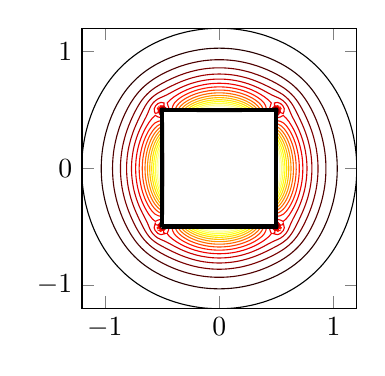
\begin{tikzpicture}

\begin{axis}[%
width=1.372in,
height=1.4in,
at={(0in,0in)},
scale only axis,
colormap/hot2,
xmin=-1.2000,
xmax=1.2000,
ymin=-1.2000,
ymax=1.2000,
axis background/.style={fill=white}
]
\addplot[contour prepared, contour prepared format=matlab, contour/labels=false] table[row sep=crcr] {%
%
0.0526	385.0000\\
-1.1816	-0.2387\\
-1.1821	-0.2363\\
-1.1864	-0.2114\\
-1.1903	-0.1866\\
-1.1935	-0.1617\\
-1.1963	-0.1368\\
-1.1986	-0.1119\\
-1.2003	-0.0871\\
-1.2017	-0.0622\\
-1.2025	-0.0373\\
-1.2029	-0.0124\\
-1.2029	0.0124\\
-1.2024	0.0373\\
-1.2014	0.0622\\
-1.2000	0.0871\\
-1.1981	0.1119\\
-1.1958	0.1368\\
-1.1929	0.1617\\
-1.1895	0.1866\\
-1.1856	0.2114\\
-1.1816	0.2337\\
-1.1812	0.2363\\
-1.1765	0.2612\\
-1.1713	0.2861\\
-1.1655	0.3109\\
-1.1590	0.3358\\
-1.1567	0.3438\\
-1.1522	0.3607\\
-1.1450	0.3856\\
-1.1369	0.4104\\
-1.1318	0.4249\\
-1.1284	0.4353\\
-1.1194	0.4602\\
-1.1096	0.4851\\
-1.1070	0.4913\\
-1.0994	0.5100\\
-1.0884	0.5348\\
-1.0821	0.5482\\
-1.0768	0.5597\\
-1.0645	0.5846\\
-1.0572	0.5983\\
-1.0515	0.6095\\
-1.0376	0.6343\\
-1.0323	0.6432\\
-1.0230	0.6592\\
-1.0075	0.6838\\
-1.0073	0.6841\\
-0.9910	0.7090\\
-0.9826	0.7209\\
-0.9735	0.7338\\
-0.9577	0.7549\\
-0.9549	0.7587\\
-0.9351	0.7836\\
-0.9328	0.7864\\
-0.9143	0.8085\\
-0.9080	0.8156\\
-0.8919	0.8333\\
-0.8831	0.8427\\
-0.8680	0.8582\\
-0.8582	0.8680\\
-0.8425	0.8831\\
-0.8333	0.8916\\
-0.8150	0.9080\\
-0.8085	0.9137\\
-0.7855	0.9328\\
-0.7836	0.9344\\
-0.7587	0.9540\\
-0.7537	0.9577\\
-0.7338	0.9725\\
-0.7192	0.9826\\
-0.7090	0.9897\\
-0.6841	1.0059\\
-0.6816	1.0075\\
-0.6592	1.0215\\
-0.6404	1.0323\\
-0.6343	1.0359\\
-0.6095	1.0497\\
-0.5948	1.0572\\
-0.5846	1.0626\\
-0.5597	1.0749\\
-0.5438	1.0821\\
-0.5348	1.0863\\
-0.5100	1.0973\\
-0.4858	1.1070\\
-0.4851	1.1073\\
-0.4602	1.1171\\
-0.4353	1.1261\\
-0.4177	1.1318\\
-0.4104	1.1344\\
-0.3856	1.1424\\
-0.3607	1.1497\\
-0.3358	1.1563\\
-0.3340	1.1567\\
-0.3109	1.1627\\
-0.2861	1.1686\\
-0.2612	1.1738\\
-0.2363	1.1784\\
-0.2169	1.1816\\
-0.2114	1.1826\\
-0.1866	1.1865\\
-0.1617	1.1899\\
-0.1368	1.1927\\
-0.1119	1.1951\\
-0.0871	1.1969\\
-0.0622	1.1983\\
-0.0373	1.1992\\
-0.0124	1.1997\\
0.0124	1.1997\\
0.0373	1.1992\\
0.0622	1.1983\\
0.0871	1.1969\\
0.1119	1.1951\\
0.1368	1.1927\\
0.1617	1.1899\\
0.1866	1.1865\\
0.2114	1.1826\\
0.2169	1.1816\\
0.2363	1.1784\\
0.2612	1.1738\\
0.2861	1.1686\\
0.3109	1.1627\\
0.3340	1.1567\\
0.3358	1.1563\\
0.3607	1.1497\\
0.3856	1.1424\\
0.4104	1.1344\\
0.4177	1.1318\\
0.4353	1.1261\\
0.4602	1.1171\\
0.4851	1.1073\\
0.4858	1.1070\\
0.5100	1.0973\\
0.5348	1.0863\\
0.5438	1.0821\\
0.5597	1.0749\\
0.5846	1.0626\\
0.5948	1.0572\\
0.6095	1.0497\\
0.6343	1.0359\\
0.6404	1.0323\\
0.6592	1.0215\\
0.6816	1.0075\\
0.6841	1.0059\\
0.7090	0.9897\\
0.7192	0.9826\\
0.7338	0.9725\\
0.7537	0.9577\\
0.7587	0.9540\\
0.7836	0.9344\\
0.7855	0.9328\\
0.8085	0.9137\\
0.8150	0.9080\\
0.8333	0.8916\\
0.8425	0.8831\\
0.8582	0.8680\\
0.8680	0.8582\\
0.8831	0.8427\\
0.8919	0.8333\\
0.9080	0.8156\\
0.9143	0.8085\\
0.9328	0.7864\\
0.9351	0.7836\\
0.9549	0.7587\\
0.9577	0.7549\\
0.9735	0.7338\\
0.9826	0.7209\\
0.9910	0.7090\\
1.0073	0.6841\\
1.0075	0.6838\\
1.0230	0.6592\\
1.0323	0.6432\\
1.0376	0.6343\\
1.0515	0.6095\\
1.0572	0.5983\\
1.0645	0.5846\\
1.0768	0.5597\\
1.0821	0.5482\\
1.0884	0.5348\\
1.0994	0.5100\\
1.1070	0.4913\\
1.1096	0.4851\\
1.1194	0.4602\\
1.1284	0.4353\\
1.1318	0.4249\\
1.1369	0.4104\\
1.1450	0.3856\\
1.1522	0.3607\\
1.1567	0.3438\\
1.1590	0.3358\\
1.1655	0.3109\\
1.1713	0.2861\\
1.1765	0.2612\\
1.1812	0.2363\\
1.1816	0.2337\\
1.1856	0.2114\\
1.1895	0.1866\\
1.1929	0.1617\\
1.1958	0.1368\\
1.1981	0.1119\\
1.2000	0.0871\\
1.2014	0.0622\\
1.2024	0.0373\\
1.2029	0.0124\\
1.2029	-0.0124\\
1.2025	-0.0373\\
1.2017	-0.0622\\
1.2003	-0.0871\\
1.1986	-0.1119\\
1.1963	-0.1368\\
1.1935	-0.1617\\
1.1903	-0.1866\\
1.1864	-0.2114\\
1.1821	-0.2363\\
1.1816	-0.2387\\
1.1775	-0.2612\\
1.1724	-0.2861\\
1.1667	-0.3109\\
1.1604	-0.3358\\
1.1567	-0.3488\\
1.1536	-0.3607\\
1.1465	-0.3856\\
1.1386	-0.4104\\
1.1318	-0.4299\\
1.1301	-0.4353\\
1.1213	-0.4602\\
1.1116	-0.4851\\
1.1070	-0.4962\\
1.1015	-0.5100\\
1.0907	-0.5348\\
1.0821	-0.5532\\
1.0791	-0.5597\\
1.0671	-0.5846\\
1.0572	-0.6033\\
1.0541	-0.6095\\
1.0405	-0.6343\\
1.0323	-0.6482\\
1.0260	-0.6592\\
1.0105	-0.6841\\
1.0075	-0.6888\\
0.9944	-0.7090\\
0.9826	-0.7259\\
0.9771	-0.7338\\
0.9586	-0.7587\\
0.9577	-0.7599\\
0.9393	-0.7836\\
0.9328	-0.7914\\
0.9186	-0.8085\\
0.9080	-0.8206\\
0.8965	-0.8333\\
0.8831	-0.8477\\
0.8730	-0.8582\\
0.8582	-0.8730\\
0.8477	-0.8831\\
0.8333	-0.8966\\
0.8207	-0.9080\\
0.8085	-0.9187\\
0.7916	-0.9328\\
0.7836	-0.9395\\
0.7602	-0.9577\\
0.7587	-0.9589\\
0.7338	-0.9774\\
0.7263	-0.9826\\
0.7090	-0.9947\\
0.6894	-1.0075\\
0.6841	-1.0109\\
0.6592	-1.0264\\
0.6489	-1.0323\\
0.6343	-1.0410\\
0.6095	-1.0546\\
0.6043	-1.0572\\
0.5846	-1.0677\\
0.5597	-1.0797\\
0.5545	-1.0821\\
0.5348	-1.0914\\
0.5100	-1.1022\\
0.4980	-1.1070\\
0.4851	-1.1124\\
0.4602	-1.1221\\
0.4353	-1.1309\\
0.4324	-1.1318\\
0.4104	-1.1395\\
0.3856	-1.1474\\
0.3607	-1.1545\\
0.3525	-1.1567\\
0.3358	-1.1614\\
0.3109	-1.1678\\
0.2861	-1.1735\\
0.2612	-1.1786\\
0.2450	-1.1816\\
0.2363	-1.1833\\
0.2114	-1.1877\\
0.1866	-1.1916\\
0.1617	-1.1949\\
0.1368	-1.1977\\
0.1119	-1.2000\\
0.0871	-1.2018\\
0.0622	-1.2031\\
0.0373	-1.2040\\
0.0124	-1.2045\\
-0.0124	-1.2045\\
-0.0373	-1.2040\\
-0.0622	-1.2031\\
-0.0871	-1.2018\\
-0.1119	-1.2000\\
-0.1368	-1.1977\\
-0.1617	-1.1949\\
-0.1866	-1.1916\\
-0.2114	-1.1877\\
-0.2363	-1.1833\\
-0.2450	-1.1816\\
-0.2612	-1.1786\\
-0.2861	-1.1735\\
-0.3109	-1.1678\\
-0.3358	-1.1614\\
-0.3525	-1.1567\\
-0.3607	-1.1545\\
-0.3856	-1.1474\\
-0.4104	-1.1395\\
-0.4324	-1.1318\\
-0.4353	-1.1309\\
-0.4602	-1.1221\\
-0.4851	-1.1124\\
-0.4980	-1.1070\\
-0.5100	-1.1022\\
-0.5348	-1.0914\\
-0.5545	-1.0821\\
-0.5597	-1.0797\\
-0.5846	-1.0677\\
-0.6043	-1.0572\\
-0.6095	-1.0546\\
-0.6343	-1.0410\\
-0.6489	-1.0323\\
-0.6592	-1.0264\\
-0.6841	-1.0109\\
-0.6894	-1.0075\\
-0.7090	-0.9947\\
-0.7263	-0.9826\\
-0.7338	-0.9774\\
-0.7587	-0.9589\\
-0.7602	-0.9577\\
-0.7836	-0.9395\\
-0.7916	-0.9328\\
-0.8085	-0.9187\\
-0.8207	-0.9080\\
-0.8333	-0.8966\\
-0.8477	-0.8831\\
-0.8582	-0.8730\\
-0.8730	-0.8582\\
-0.8831	-0.8477\\
-0.8965	-0.8333\\
-0.9080	-0.8206\\
-0.9186	-0.8085\\
-0.9328	-0.7914\\
-0.9393	-0.7836\\
-0.9577	-0.7599\\
-0.9586	-0.7587\\
-0.9771	-0.7338\\
-0.9826	-0.7259\\
-0.9944	-0.7090\\
-1.0075	-0.6888\\
-1.0105	-0.6841\\
-1.0260	-0.6592\\
-1.0323	-0.6482\\
-1.0405	-0.6343\\
-1.0541	-0.6095\\
-1.0572	-0.6033\\
-1.0671	-0.5846\\
-1.0791	-0.5597\\
-1.0821	-0.5532\\
-1.0907	-0.5348\\
-1.1015	-0.5100\\
-1.1070	-0.4962\\
-1.1116	-0.4851\\
-1.1213	-0.4602\\
-1.1301	-0.4353\\
-1.1318	-0.4299\\
-1.1386	-0.4104\\
-1.1465	-0.3856\\
-1.1536	-0.3607\\
-1.1567	-0.3488\\
-1.1604	-0.3358\\
-1.1667	-0.3109\\
-1.1724	-0.2861\\
-1.1775	-0.2612\\
-1.1816	-0.2387\\
0.0526	177.0000\\
-0.5100	-0.4810\\
-0.5136	-0.4851\\
-0.5129	-0.5100\\
-0.5100	-0.5129\\
-0.4851	-0.5136\\
-0.4810	-0.5100\\
-0.4602	-0.4892\\
-0.4353	-0.4885\\
-0.4104	-0.4882\\
-0.3856	-0.4878\\
-0.3607	-0.4876\\
-0.3358	-0.4874\\
-0.3109	-0.4872\\
-0.2861	-0.4870\\
-0.2612	-0.4869\\
-0.2363	-0.4868\\
-0.2114	-0.4867\\
-0.1866	-0.4866\\
-0.1617	-0.4866\\
-0.1368	-0.4865\\
-0.1119	-0.4865\\
-0.0871	-0.4864\\
-0.0622	-0.4864\\
-0.0373	-0.4864\\
-0.0124	-0.4864\\
0.0124	-0.4864\\
0.0373	-0.4864\\
0.0622	-0.4864\\
0.0871	-0.4864\\
0.1119	-0.4865\\
0.1368	-0.4865\\
0.1617	-0.4866\\
0.1866	-0.4866\\
0.2114	-0.4867\\
0.2363	-0.4868\\
0.2612	-0.4869\\
0.2861	-0.4870\\
0.3109	-0.4872\\
0.3358	-0.4874\\
0.3607	-0.4876\\
0.3856	-0.4878\\
0.4104	-0.4882\\
0.4353	-0.4885\\
0.4602	-0.4892\\
0.4810	-0.5100\\
0.4851	-0.5136\\
0.5100	-0.5129\\
0.5129	-0.5100\\
0.5136	-0.4851\\
0.5100	-0.4810\\
0.4892	-0.4602\\
0.4886	-0.4353\\
0.4882	-0.4104\\
0.4878	-0.3856\\
0.4876	-0.3607\\
0.4874	-0.3358\\
0.4872	-0.3109\\
0.4870	-0.2861\\
0.4869	-0.2612\\
0.4868	-0.2363\\
0.4867	-0.2114\\
0.4866	-0.1866\\
0.4866	-0.1617\\
0.4865	-0.1368\\
0.4865	-0.1119\\
0.4864	-0.0871\\
0.4864	-0.0622\\
0.4864	-0.0373\\
0.4864	-0.0124\\
0.4864	0.0124\\
0.4864	0.0373\\
0.4864	0.0622\\
0.4864	0.0871\\
0.4865	0.1119\\
0.4865	0.1368\\
0.4866	0.1617\\
0.4866	0.1866\\
0.4867	0.2114\\
0.4868	0.2363\\
0.4869	0.2612\\
0.4871	0.2861\\
0.4872	0.3109\\
0.4874	0.3358\\
0.4876	0.3607\\
0.4879	0.3856\\
0.4882	0.4104\\
0.4886	0.4353\\
0.4894	0.4602\\
0.5100	0.4807\\
0.5134	0.4851\\
0.5130	0.5100\\
0.5100	0.5130\\
0.4851	0.5135\\
0.4810	0.5100\\
0.4602	0.4892\\
0.4353	0.4885\\
0.4104	0.4882\\
0.3856	0.4879\\
0.3607	0.4876\\
0.3358	0.4874\\
0.3109	0.4872\\
0.2861	0.4871\\
0.2612	0.4869\\
0.2363	0.4868\\
0.2114	0.4867\\
0.1866	0.4866\\
0.1617	0.4866\\
0.1368	0.4865\\
0.1119	0.4865\\
0.0871	0.4865\\
0.0622	0.4864\\
0.0373	0.4864\\
0.0124	0.4864\\
-0.0124	0.4864\\
-0.0373	0.4864\\
-0.0622	0.4864\\
-0.0871	0.4865\\
-0.1119	0.4865\\
-0.1368	0.4865\\
-0.1617	0.4866\\
-0.1866	0.4866\\
-0.2114	0.4867\\
-0.2363	0.4868\\
-0.2612	0.4869\\
-0.2861	0.4871\\
-0.3109	0.4872\\
-0.3358	0.4874\\
-0.3607	0.4876\\
-0.3856	0.4879\\
-0.4104	0.4882\\
-0.4353	0.4885\\
-0.4602	0.4892\\
-0.4810	0.5100\\
-0.4851	0.5135\\
-0.5100	0.5130\\
-0.5130	0.5100\\
-0.5134	0.4851\\
-0.5100	0.4807\\
-0.4894	0.4602\\
-0.4886	0.4353\\
-0.4882	0.4104\\
-0.4879	0.3856\\
-0.4876	0.3607\\
-0.4874	0.3358\\
-0.4872	0.3109\\
-0.4871	0.2861\\
-0.4869	0.2612\\
-0.4868	0.2363\\
-0.4867	0.2114\\
-0.4866	0.1866\\
-0.4866	0.1617\\
-0.4865	0.1368\\
-0.4865	0.1119\\
-0.4864	0.0871\\
-0.4864	0.0622\\
-0.4864	0.0373\\
-0.4864	0.0124\\
-0.4864	-0.0124\\
-0.4864	-0.0373\\
-0.4864	-0.0622\\
-0.4864	-0.0871\\
-0.4865	-0.1119\\
-0.4865	-0.1368\\
-0.4866	-0.1617\\
-0.4866	-0.1866\\
-0.4867	-0.2114\\
-0.4868	-0.2363\\
-0.4869	-0.2612\\
-0.4870	-0.2861\\
-0.4872	-0.3109\\
-0.4874	-0.3358\\
-0.4876	-0.3607\\
-0.4878	-0.3856\\
-0.4882	-0.4104\\
-0.4886	-0.4353\\
-0.4892	-0.4602\\
-0.5100	-0.4810\\
0.1053	331.0000\\
-1.0075	-0.2398\\
-1.0082	-0.2363\\
-1.0132	-0.2114\\
-1.0176	-0.1866\\
-1.0213	-0.1617\\
-1.0245	-0.1368\\
-1.0270	-0.1119\\
-1.0291	-0.0871\\
-1.0306	-0.0622\\
-1.0315	-0.0373\\
-1.0320	-0.0124\\
-1.0319	0.0124\\
-1.0314	0.0373\\
-1.0303	0.0622\\
-1.0287	0.0871\\
-1.0266	0.1119\\
-1.0239	0.1368\\
-1.0206	0.1617\\
-1.0168	0.1866\\
-1.0123	0.2114\\
-1.0075	0.2348\\
-1.0072	0.2363\\
-1.0019	0.2612\\
-0.9959	0.2861\\
-0.9892	0.3109\\
-0.9826	0.3328\\
-0.9817	0.3358\\
-0.9741	0.3607\\
-0.9657	0.3856\\
-0.9577	0.4067\\
-0.9564	0.4104\\
-0.9469	0.4353\\
-0.9363	0.4602\\
-0.9328	0.4678\\
-0.9253	0.4851\\
-0.9133	0.5100\\
-0.9080	0.5203\\
-0.9007	0.5348\\
-0.8870	0.5597\\
-0.8831	0.5664\\
-0.8726	0.5846\\
-0.8582	0.6073\\
-0.8569	0.6095\\
-0.8403	0.6343\\
-0.8333	0.6440\\
-0.8224	0.6592\\
-0.8085	0.6770\\
-0.8029	0.6841\\
-0.7836	0.7068\\
-0.7817	0.7090\\
-0.7587	0.7338\\
-0.7587	0.7338\\
-0.7338	0.7585\\
-0.7337	0.7587\\
-0.7090	0.7812\\
-0.7062	0.7836\\
-0.6841	0.8021\\
-0.6759	0.8085\\
-0.6592	0.8214\\
-0.6424	0.8333\\
-0.6343	0.8391\\
-0.6095	0.8555\\
-0.6051	0.8582\\
-0.5846	0.8710\\
-0.5634	0.8831\\
-0.5597	0.8852\\
-0.5348	0.8988\\
-0.5164	0.9080\\
-0.5100	0.9113\\
-0.4851	0.9232\\
-0.4629	0.9328\\
-0.4602	0.9341\\
-0.4353	0.9446\\
-0.4104	0.9542\\
-0.4004	0.9577\\
-0.3856	0.9632\\
-0.3607	0.9717\\
-0.3358	0.9793\\
-0.3241	0.9826\\
-0.3109	0.9865\\
-0.2861	0.9932\\
-0.2612	0.9992\\
-0.2363	1.0045\\
-0.2208	1.0075\\
-0.2114	1.0094\\
-0.1866	1.0138\\
-0.1617	1.0177\\
-0.1368	1.0209\\
-0.1119	1.0236\\
-0.0871	1.0257\\
-0.0622	1.0273\\
-0.0373	1.0283\\
-0.0124	1.0288\\
0.0124	1.0288\\
0.0373	1.0283\\
0.0622	1.0273\\
0.0871	1.0257\\
0.1119	1.0236\\
0.1368	1.0209\\
0.1617	1.0177\\
0.1866	1.0138\\
0.2114	1.0094\\
0.2208	1.0075\\
0.2363	1.0045\\
0.2612	0.9992\\
0.2861	0.9932\\
0.3109	0.9865\\
0.3241	0.9826\\
0.3358	0.9793\\
0.3607	0.9717\\
0.3856	0.9632\\
0.4004	0.9577\\
0.4104	0.9542\\
0.4353	0.9446\\
0.4602	0.9341\\
0.4629	0.9328\\
0.4851	0.9232\\
0.5100	0.9113\\
0.5164	0.9080\\
0.5348	0.8988\\
0.5597	0.8852\\
0.5634	0.8831\\
0.5846	0.8710\\
0.6051	0.8582\\
0.6095	0.8555\\
0.6343	0.8391\\
0.6424	0.8333\\
0.6592	0.8214\\
0.6759	0.8085\\
0.6841	0.8021\\
0.7062	0.7836\\
0.7090	0.7812\\
0.7337	0.7587\\
0.7338	0.7585\\
0.7587	0.7338\\
0.7587	0.7338\\
0.7817	0.7090\\
0.7836	0.7068\\
0.8029	0.6841\\
0.8085	0.6770\\
0.8224	0.6592\\
0.8333	0.6440\\
0.8403	0.6343\\
0.8569	0.6095\\
0.8582	0.6073\\
0.8726	0.5846\\
0.8831	0.5664\\
0.8870	0.5597\\
0.9007	0.5348\\
0.9080	0.5203\\
0.9133	0.5100\\
0.9253	0.4851\\
0.9328	0.4678\\
0.9363	0.4602\\
0.9469	0.4353\\
0.9564	0.4104\\
0.9577	0.4067\\
0.9657	0.3856\\
0.9741	0.3607\\
0.9817	0.3358\\
0.9826	0.3328\\
0.9892	0.3109\\
0.9959	0.2861\\
1.0019	0.2612\\
1.0072	0.2363\\
1.0075	0.2348\\
1.0123	0.2114\\
1.0168	0.1866\\
1.0206	0.1617\\
1.0239	0.1368\\
1.0266	0.1119\\
1.0287	0.0871\\
1.0303	0.0622\\
1.0314	0.0373\\
1.0319	0.0124\\
1.0320	-0.0124\\
1.0315	-0.0373\\
1.0306	-0.0622\\
1.0291	-0.0871\\
1.0270	-0.1119\\
1.0245	-0.1368\\
1.0213	-0.1617\\
1.0176	-0.1866\\
1.0132	-0.2114\\
1.0082	-0.2363\\
1.0075	-0.2398\\
1.0030	-0.2612\\
0.9971	-0.2861\\
0.9906	-0.3109\\
0.9832	-0.3358\\
0.9826	-0.3378\\
0.9757	-0.3607\\
0.9674	-0.3856\\
0.9582	-0.4104\\
0.9577	-0.4117\\
0.9488	-0.4353\\
0.9385	-0.4602\\
0.9328	-0.4727\\
0.9275	-0.4851\\
0.9158	-0.5100\\
0.9080	-0.5253\\
0.9032	-0.5348\\
0.8899	-0.5597\\
0.8831	-0.5714\\
0.8756	-0.5846\\
0.8601	-0.6095\\
0.8582	-0.6123\\
0.8438	-0.6343\\
0.8333	-0.6490\\
0.8261	-0.6592\\
0.8085	-0.6819\\
0.8068	-0.6841\\
0.7861	-0.7090\\
0.7836	-0.7118\\
0.7636	-0.7338\\
0.7587	-0.7389\\
0.7390	-0.7587\\
0.7338	-0.7636\\
0.7119	-0.7836\\
0.7090	-0.7862\\
0.6841	-0.8070\\
0.6822	-0.8085\\
0.6592	-0.8263\\
0.6494	-0.8333\\
0.6343	-0.8441\\
0.6128	-0.8582\\
0.6095	-0.8605\\
0.5846	-0.8760\\
0.5721	-0.8831\\
0.5597	-0.8903\\
0.5348	-0.9037\\
0.5263	-0.9080\\
0.5100	-0.9164\\
0.4851	-0.9281\\
0.4742	-0.9328\\
0.4602	-0.9392\\
0.4353	-0.9496\\
0.4138	-0.9577\\
0.4104	-0.9590\\
0.3856	-0.9683\\
0.3607	-0.9766\\
0.3409	-0.9826\\
0.3358	-0.9842\\
0.3109	-0.9916\\
0.2861	-0.9982\\
0.2612	-1.0041\\
0.2452	-1.0075\\
0.2363	-1.0095\\
0.2114	-1.0145\\
0.1866	-1.0189\\
0.1617	-1.0227\\
0.1368	-1.0258\\
0.1119	-1.0284\\
0.0871	-1.0305\\
0.0622	-1.0320\\
0.0550	-1.0323\\
0.0373	-1.0331\\
0.0124	-1.0337\\
-0.0124	-1.0337\\
-0.0373	-1.0331\\
-0.0550	-1.0323\\
-0.0622	-1.0320\\
-0.0871	-1.0305\\
-0.1119	-1.0284\\
-0.1368	-1.0258\\
-0.1617	-1.0227\\
-0.1866	-1.0189\\
-0.2114	-1.0145\\
-0.2363	-1.0095\\
-0.2452	-1.0075\\
-0.2612	-1.0041\\
-0.2861	-0.9982\\
-0.3109	-0.9916\\
-0.3358	-0.9842\\
-0.3409	-0.9826\\
-0.3607	-0.9766\\
-0.3856	-0.9683\\
-0.4104	-0.9590\\
-0.4138	-0.9577\\
-0.4353	-0.9496\\
-0.4602	-0.9392\\
-0.4742	-0.9328\\
-0.4851	-0.9281\\
-0.5100	-0.9164\\
-0.5263	-0.9080\\
-0.5348	-0.9037\\
-0.5597	-0.8903\\
-0.5721	-0.8831\\
-0.5846	-0.8760\\
-0.6095	-0.8605\\
-0.6128	-0.8582\\
-0.6343	-0.8441\\
-0.6494	-0.8333\\
-0.6592	-0.8263\\
-0.6822	-0.8085\\
-0.6841	-0.8070\\
-0.7090	-0.7862\\
-0.7119	-0.7836\\
-0.7338	-0.7636\\
-0.7390	-0.7587\\
-0.7587	-0.7389\\
-0.7636	-0.7338\\
-0.7836	-0.7118\\
-0.7861	-0.7090\\
-0.8068	-0.6841\\
-0.8085	-0.6819\\
-0.8261	-0.6592\\
-0.8333	-0.6490\\
-0.8438	-0.6343\\
-0.8582	-0.6123\\
-0.8601	-0.6095\\
-0.8756	-0.5846\\
-0.8831	-0.5714\\
-0.8899	-0.5597\\
-0.9032	-0.5348\\
-0.9080	-0.5253\\
-0.9158	-0.5100\\
-0.9275	-0.4851\\
-0.9328	-0.4727\\
-0.9385	-0.4602\\
-0.9488	-0.4353\\
-0.9577	-0.4117\\
-0.9582	-0.4104\\
-0.9674	-0.3856\\
-0.9757	-0.3607\\
-0.9826	-0.3378\\
-0.9832	-0.3358\\
-0.9906	-0.3109\\
-0.9971	-0.2861\\
-1.0030	-0.2612\\
-1.0075	-0.2398\\
0.1053	177.0000\\
-0.5100	-0.4768\\
-0.5172	-0.4851\\
-0.5159	-0.5100\\
-0.5100	-0.5159\\
-0.4851	-0.5172\\
-0.4769	-0.5100\\
-0.4602	-0.4933\\
-0.4353	-0.4920\\
-0.4104	-0.4912\\
-0.3856	-0.4906\\
-0.3607	-0.4901\\
-0.3358	-0.4896\\
-0.3109	-0.4893\\
-0.2861	-0.4890\\
-0.2612	-0.4887\\
-0.2363	-0.4885\\
-0.2114	-0.4883\\
-0.1866	-0.4882\\
-0.1617	-0.4880\\
-0.1368	-0.4879\\
-0.1119	-0.4878\\
-0.0871	-0.4878\\
-0.0622	-0.4877\\
-0.0373	-0.4877\\
-0.0124	-0.4877\\
0.0124	-0.4877\\
0.0373	-0.4877\\
0.0622	-0.4877\\
0.0871	-0.4878\\
0.1119	-0.4878\\
0.1368	-0.4879\\
0.1617	-0.4880\\
0.1866	-0.4882\\
0.2114	-0.4883\\
0.2363	-0.4885\\
0.2612	-0.4887\\
0.2861	-0.4890\\
0.3109	-0.4893\\
0.3358	-0.4896\\
0.3607	-0.4901\\
0.3856	-0.4906\\
0.4104	-0.4912\\
0.4353	-0.4920\\
0.4602	-0.4933\\
0.4769	-0.5100\\
0.4851	-0.5172\\
0.5100	-0.5159\\
0.5159	-0.5100\\
0.5172	-0.4851\\
0.5100	-0.4768\\
0.4933	-0.4602\\
0.4920	-0.4353\\
0.4912	-0.4104\\
0.4906	-0.3856\\
0.4901	-0.3607\\
0.4896	-0.3358\\
0.4893	-0.3109\\
0.4890	-0.2861\\
0.4887	-0.2612\\
0.4885	-0.2363\\
0.4883	-0.2114\\
0.4882	-0.1866\\
0.4880	-0.1617\\
0.4879	-0.1368\\
0.4879	-0.1119\\
0.4878	-0.0871\\
0.4878	-0.0622\\
0.4877	-0.0373\\
0.4877	-0.0124\\
0.4877	0.0124\\
0.4877	0.0373\\
0.4878	0.0622\\
0.4878	0.0871\\
0.4879	0.1119\\
0.4880	0.1368\\
0.4881	0.1617\\
0.4882	0.1866\\
0.4884	0.2114\\
0.4885	0.2363\\
0.4888	0.2612\\
0.4890	0.2861\\
0.4893	0.3109\\
0.4897	0.3358\\
0.4902	0.3607\\
0.4907	0.3856\\
0.4914	0.4104\\
0.4922	0.4353\\
0.4938	0.4602\\
0.5100	0.4763\\
0.5168	0.4851\\
0.5160	0.5100\\
0.5100	0.5161\\
0.4851	0.5170\\
0.4769	0.5100\\
0.4602	0.4933\\
0.4353	0.4920\\
0.4104	0.4913\\
0.3856	0.4906\\
0.3607	0.4901\\
0.3358	0.4897\\
0.3109	0.4893\\
0.2861	0.4890\\
0.2612	0.4888\\
0.2363	0.4886\\
0.2114	0.4884\\
0.1866	0.4882\\
0.1617	0.4881\\
0.1368	0.4880\\
0.1119	0.4879\\
0.0871	0.4878\\
0.0622	0.4878\\
0.0373	0.4878\\
0.0124	0.4878\\
-0.0124	0.4878\\
-0.0373	0.4878\\
-0.0622	0.4878\\
-0.0871	0.4878\\
-0.1119	0.4879\\
-0.1368	0.4880\\
-0.1617	0.4881\\
-0.1866	0.4882\\
-0.2114	0.4884\\
-0.2363	0.4886\\
-0.2612	0.4888\\
-0.2861	0.4890\\
-0.3109	0.4893\\
-0.3358	0.4897\\
-0.3607	0.4901\\
-0.3856	0.4906\\
-0.4104	0.4913\\
-0.4353	0.4920\\
-0.4602	0.4933\\
-0.4769	0.5100\\
-0.4851	0.5170\\
-0.5100	0.5161\\
-0.5160	0.5100\\
-0.5168	0.4851\\
-0.5100	0.4763\\
-0.4938	0.4602\\
-0.4922	0.4353\\
-0.4914	0.4104\\
-0.4907	0.3856\\
-0.4902	0.3607\\
-0.4897	0.3358\\
-0.4893	0.3109\\
-0.4890	0.2861\\
-0.4888	0.2612\\
-0.4885	0.2363\\
-0.4884	0.2114\\
-0.4882	0.1866\\
-0.4881	0.1617\\
-0.4880	0.1368\\
-0.4879	0.1119\\
-0.4878	0.0871\\
-0.4878	0.0622\\
-0.4877	0.0373\\
-0.4877	0.0124\\
-0.4877	-0.0124\\
-0.4877	-0.0373\\
-0.4878	-0.0622\\
-0.4878	-0.0871\\
-0.4879	-0.1119\\
-0.4879	-0.1368\\
-0.4880	-0.1617\\
-0.4882	-0.1866\\
-0.4883	-0.2114\\
-0.4885	-0.2363\\
-0.4887	-0.2612\\
-0.4890	-0.2861\\
-0.4893	-0.3109\\
-0.4896	-0.3358\\
-0.4901	-0.3607\\
-0.4906	-0.3856\\
-0.4912	-0.4104\\
-0.4920	-0.4353\\
-0.4933	-0.4602\\
-0.5100	-0.4768\\
0.1579	303.0000\\
-0.9328	-0.0264\\
-0.9332	-0.0124\\
-0.9331	0.0124\\
-0.9328	0.0216\\
-0.9324	0.0373\\
-0.9313	0.0622\\
-0.9295	0.0871\\
-0.9271	0.1119\\
-0.9241	0.1368\\
-0.9205	0.1617\\
-0.9162	0.1866\\
-0.9112	0.2114\\
-0.9080	0.2257\\
-0.9057	0.2363\\
-0.8998	0.2612\\
-0.8931	0.2861\\
-0.8855	0.3109\\
-0.8831	0.3184\\
-0.8777	0.3358\\
-0.8691	0.3607\\
-0.8596	0.3856\\
-0.8582	0.3890\\
-0.8499	0.4104\\
-0.8392	0.4353\\
-0.8333	0.4480\\
-0.8279	0.4602\\
-0.8158	0.4851\\
-0.8085	0.4990\\
-0.8029	0.5100\\
-0.7890	0.5348\\
-0.7836	0.5439\\
-0.7742	0.5597\\
-0.7587	0.5833\\
-0.7579	0.5846\\
-0.7404	0.6095\\
-0.7338	0.6179\\
-0.7210	0.6343\\
-0.7090	0.6484\\
-0.6994	0.6592\\
-0.6841	0.6752\\
-0.6751	0.6841\\
-0.6592	0.6990\\
-0.6477	0.7090\\
-0.6343	0.7202\\
-0.6166	0.7338\\
-0.6095	0.7393\\
-0.5846	0.7565\\
-0.5812	0.7587\\
-0.5597	0.7727\\
-0.5410	0.7836\\
-0.5348	0.7873\\
-0.5100	0.8011\\
-0.4953	0.8085\\
-0.4851	0.8138\\
-0.4602	0.8259\\
-0.4433	0.8333\\
-0.4353	0.8370\\
-0.4104	0.8477\\
-0.3856	0.8573\\
-0.3832	0.8582\\
-0.3607	0.8668\\
-0.3358	0.8753\\
-0.3109	0.8830\\
-0.3106	0.8831\\
-0.2861	0.8905\\
-0.2612	0.8972\\
-0.2363	0.9031\\
-0.2133	0.9080\\
-0.2114	0.9084\\
-0.1866	0.9134\\
-0.1617	0.9177\\
-0.1368	0.9213\\
-0.1119	0.9242\\
-0.0871	0.9266\\
-0.0622	0.9283\\
-0.0373	0.9294\\
-0.0124	0.9300\\
0.0124	0.9300\\
0.0373	0.9294\\
0.0622	0.9283\\
0.0871	0.9266\\
0.1119	0.9242\\
0.1368	0.9213\\
0.1617	0.9177\\
0.1866	0.9134\\
0.2114	0.9084\\
0.2133	0.9080\\
0.2363	0.9031\\
0.2612	0.8972\\
0.2861	0.8905\\
0.3106	0.8831\\
0.3109	0.8830\\
0.3358	0.8753\\
0.3607	0.8668\\
0.3832	0.8582\\
0.3856	0.8573\\
0.4104	0.8477\\
0.4353	0.8370\\
0.4433	0.8333\\
0.4602	0.8259\\
0.4851	0.8138\\
0.4953	0.8085\\
0.5100	0.8011\\
0.5348	0.7873\\
0.5410	0.7836\\
0.5597	0.7727\\
0.5812	0.7587\\
0.5846	0.7565\\
0.6095	0.7393\\
0.6166	0.7338\\
0.6343	0.7202\\
0.6477	0.7090\\
0.6592	0.6990\\
0.6751	0.6841\\
0.6841	0.6752\\
0.6994	0.6592\\
0.7090	0.6484\\
0.7210	0.6343\\
0.7338	0.6179\\
0.7404	0.6095\\
0.7579	0.5846\\
0.7587	0.5833\\
0.7742	0.5597\\
0.7836	0.5439\\
0.7890	0.5348\\
0.8029	0.5100\\
0.8085	0.4990\\
0.8158	0.4851\\
0.8279	0.4602\\
0.8333	0.4480\\
0.8392	0.4353\\
0.8499	0.4104\\
0.8582	0.3890\\
0.8596	0.3856\\
0.8691	0.3607\\
0.8777	0.3358\\
0.8831	0.3184\\
0.8855	0.3109\\
0.8931	0.2861\\
0.8998	0.2612\\
0.9057	0.2363\\
0.9080	0.2257\\
0.9112	0.2114\\
0.9162	0.1866\\
0.9205	0.1617\\
0.9241	0.1368\\
0.9271	0.1119\\
0.9295	0.0871\\
0.9313	0.0622\\
0.9324	0.0373\\
0.9328	0.0216\\
0.9331	0.0124\\
0.9332	-0.0124\\
0.9328	-0.0264\\
0.9326	-0.0373\\
0.9315	-0.0622\\
0.9299	-0.0871\\
0.9276	-0.1119\\
0.9248	-0.1368\\
0.9213	-0.1617\\
0.9171	-0.1866\\
0.9123	-0.2114\\
0.9080	-0.2307\\
0.9068	-0.2363\\
0.9010	-0.2612\\
0.8945	-0.2861\\
0.8871	-0.3109\\
0.8831	-0.3233\\
0.8793	-0.3358\\
0.8709	-0.3607\\
0.8616	-0.3856\\
0.8582	-0.3940\\
0.8519	-0.4104\\
0.8414	-0.4353\\
0.8333	-0.4530\\
0.8301	-0.4602\\
0.8183	-0.4851\\
0.8085	-0.5040\\
0.8055	-0.5100\\
0.7919	-0.5348\\
0.7836	-0.5488\\
0.7772	-0.5597\\
0.7613	-0.5846\\
0.7587	-0.5883\\
0.7441	-0.6095\\
0.7338	-0.6229\\
0.7250	-0.6343\\
0.7090	-0.6533\\
0.7038	-0.6592\\
0.6841	-0.6801\\
0.6801	-0.6841\\
0.6592	-0.7039\\
0.6534	-0.7090\\
0.6343	-0.7252\\
0.6231	-0.7338\\
0.6095	-0.7443\\
0.5887	-0.7587\\
0.5846	-0.7615\\
0.5597	-0.7776\\
0.5494	-0.7836\\
0.5348	-0.7924\\
0.5100	-0.8059\\
0.5049	-0.8085\\
0.4851	-0.8189\\
0.4602	-0.8307\\
0.4543	-0.8333\\
0.4353	-0.8421\\
0.4104	-0.8526\\
0.3960	-0.8582\\
0.3856	-0.8624\\
0.3607	-0.8718\\
0.3358	-0.8802\\
0.3264	-0.8831\\
0.3109	-0.8881\\
0.2861	-0.8955\\
0.2612	-0.9021\\
0.2363	-0.9079\\
0.2361	-0.9080\\
0.2114	-0.9135\\
0.1866	-0.9184\\
0.1617	-0.9226\\
0.1368	-0.9262\\
0.1119	-0.9291\\
0.0871	-0.9314\\
0.0653	-0.9328\\
0.0622	-0.9331\\
0.0373	-0.9343\\
0.0124	-0.9349\\
-0.0124	-0.9349\\
-0.0373	-0.9343\\
-0.0622	-0.9331\\
-0.0653	-0.9328\\
-0.0871	-0.9314\\
-0.1119	-0.9291\\
-0.1368	-0.9262\\
-0.1617	-0.9226\\
-0.1866	-0.9184\\
-0.2114	-0.9135\\
-0.2361	-0.9080\\
-0.2363	-0.9079\\
-0.2612	-0.9021\\
-0.2861	-0.8955\\
-0.3109	-0.8881\\
-0.3264	-0.8831\\
-0.3358	-0.8802\\
-0.3607	-0.8718\\
-0.3856	-0.8624\\
-0.3960	-0.8582\\
-0.4104	-0.8526\\
-0.4353	-0.8421\\
-0.4543	-0.8333\\
-0.4602	-0.8307\\
-0.4851	-0.8189\\
-0.5049	-0.8085\\
-0.5100	-0.8059\\
-0.5348	-0.7924\\
-0.5494	-0.7836\\
-0.5597	-0.7776\\
-0.5846	-0.7615\\
-0.5887	-0.7587\\
-0.6095	-0.7443\\
-0.6231	-0.7338\\
-0.6343	-0.7252\\
-0.6534	-0.7090\\
-0.6592	-0.7039\\
-0.6801	-0.6841\\
-0.6841	-0.6801\\
-0.7038	-0.6592\\
-0.7090	-0.6533\\
-0.7250	-0.6343\\
-0.7338	-0.6229\\
-0.7441	-0.6095\\
-0.7587	-0.5883\\
-0.7613	-0.5846\\
-0.7772	-0.5597\\
-0.7836	-0.5488\\
-0.7919	-0.5348\\
-0.8055	-0.5100\\
-0.8085	-0.5040\\
-0.8183	-0.4851\\
-0.8301	-0.4602\\
-0.8333	-0.4530\\
-0.8414	-0.4353\\
-0.8519	-0.4104\\
-0.8582	-0.3940\\
-0.8616	-0.3856\\
-0.8709	-0.3607\\
-0.8793	-0.3358\\
-0.8831	-0.3233\\
-0.8871	-0.3109\\
-0.8945	-0.2861\\
-0.9010	-0.2612\\
-0.9068	-0.2363\\
-0.9080	-0.2307\\
-0.9123	-0.2114\\
-0.9171	-0.1866\\
-0.9213	-0.1617\\
-0.9248	-0.1368\\
-0.9276	-0.1119\\
-0.9299	-0.0871\\
-0.9315	-0.0622\\
-0.9326	-0.0373\\
-0.9328	-0.0264\\
0.1579	177.0000\\
-0.5100	-0.4727\\
-0.5208	-0.4851\\
-0.5189	-0.5100\\
-0.5100	-0.5189\\
-0.4851	-0.5208\\
-0.4728	-0.5100\\
-0.4602	-0.4974\\
-0.4353	-0.4955\\
-0.4104	-0.4943\\
-0.3856	-0.4934\\
-0.3607	-0.4926\\
-0.3358	-0.4919\\
-0.3109	-0.4914\\
-0.2861	-0.4909\\
-0.2612	-0.4905\\
-0.2363	-0.4902\\
-0.2114	-0.4899\\
-0.1866	-0.4897\\
-0.1617	-0.4895\\
-0.1368	-0.4894\\
-0.1119	-0.4892\\
-0.0871	-0.4891\\
-0.0622	-0.4891\\
-0.0373	-0.4890\\
-0.0124	-0.4890\\
0.0124	-0.4890\\
0.0373	-0.4890\\
0.0622	-0.4891\\
0.0871	-0.4891\\
0.1119	-0.4892\\
0.1368	-0.4894\\
0.1617	-0.4895\\
0.1866	-0.4897\\
0.2114	-0.4899\\
0.2363	-0.4902\\
0.2612	-0.4905\\
0.2861	-0.4909\\
0.3109	-0.4914\\
0.3358	-0.4919\\
0.3607	-0.4926\\
0.3856	-0.4934\\
0.4104	-0.4943\\
0.4353	-0.4955\\
0.4602	-0.4974\\
0.4728	-0.5100\\
0.4851	-0.5208\\
0.5100	-0.5189\\
0.5189	-0.5100\\
0.5208	-0.4851\\
0.5100	-0.4727\\
0.4974	-0.4602\\
0.4955	-0.4353\\
0.4943	-0.4104\\
0.4934	-0.3856\\
0.4926	-0.3607\\
0.4919	-0.3358\\
0.4914	-0.3109\\
0.4909	-0.2861\\
0.4905	-0.2612\\
0.4902	-0.2363\\
0.4899	-0.2114\\
0.4897	-0.1866\\
0.4895	-0.1617\\
0.4894	-0.1368\\
0.4893	-0.1119\\
0.4892	-0.0871\\
0.4891	-0.0622\\
0.4891	-0.0373\\
0.4890	-0.0124\\
0.4890	0.0124\\
0.4891	0.0373\\
0.4891	0.0622\\
0.4892	0.0871\\
0.4893	0.1119\\
0.4894	0.1368\\
0.4896	0.1617\\
0.4898	0.1866\\
0.4900	0.2114\\
0.4903	0.2363\\
0.4906	0.2612\\
0.4910	0.2861\\
0.4915	0.3109\\
0.4920	0.3358\\
0.4927	0.3607\\
0.4936	0.3856\\
0.4945	0.4104\\
0.4958	0.4353\\
0.4982	0.4602\\
0.5100	0.4720\\
0.5203	0.4851\\
0.5190	0.5100\\
0.5100	0.5192\\
0.4851	0.5206\\
0.4728	0.5100\\
0.4602	0.4974\\
0.4353	0.4955\\
0.4104	0.4943\\
0.3856	0.4934\\
0.3607	0.4927\\
0.3358	0.4920\\
0.3109	0.4915\\
0.2861	0.4910\\
0.2612	0.4906\\
0.2363	0.4903\\
0.2114	0.4900\\
0.1866	0.4898\\
0.1617	0.4896\\
0.1368	0.4895\\
0.1119	0.4893\\
0.0871	0.4892\\
0.0622	0.4892\\
0.0373	0.4891\\
0.0124	0.4891\\
-0.0124	0.4891\\
-0.0373	0.4891\\
-0.0622	0.4892\\
-0.0871	0.4892\\
-0.1119	0.4893\\
-0.1368	0.4895\\
-0.1617	0.4896\\
-0.1866	0.4898\\
-0.2114	0.4900\\
-0.2363	0.4903\\
-0.2612	0.4906\\
-0.2861	0.4910\\
-0.3109	0.4915\\
-0.3358	0.4920\\
-0.3607	0.4927\\
-0.3856	0.4934\\
-0.4104	0.4943\\
-0.4353	0.4955\\
-0.4602	0.4974\\
-0.4728	0.5100\\
-0.4851	0.5206\\
-0.5100	0.5192\\
-0.5190	0.5100\\
-0.5203	0.4851\\
-0.5100	0.4720\\
-0.4982	0.4602\\
-0.4958	0.4353\\
-0.4945	0.4104\\
-0.4936	0.3856\\
-0.4927	0.3607\\
-0.4920	0.3358\\
-0.4915	0.3109\\
-0.4910	0.2861\\
-0.4906	0.2612\\
-0.4903	0.2363\\
-0.4900	0.2114\\
-0.4898	0.1866\\
-0.4896	0.1617\\
-0.4894	0.1368\\
-0.4893	0.1119\\
-0.4892	0.0871\\
-0.4891	0.0622\\
-0.4891	0.0373\\
-0.4890	0.0124\\
-0.4890	-0.0124\\
-0.4891	-0.0373\\
-0.4891	-0.0622\\
-0.4892	-0.0871\\
-0.4893	-0.1119\\
-0.4894	-0.1368\\
-0.4895	-0.1617\\
-0.4897	-0.1866\\
-0.4899	-0.2114\\
-0.4902	-0.2363\\
-0.4905	-0.2612\\
-0.4909	-0.2861\\
-0.4914	-0.3109\\
-0.4919	-0.3358\\
-0.4926	-0.3607\\
-0.4934	-0.3856\\
-0.4943	-0.4104\\
-0.4955	-0.4353\\
-0.4974	-0.4602\\
-0.5100	-0.4727\\
0.2105	281.0000\\
-0.8582	-0.1040\\
-0.8600	-0.0871\\
-0.8620	-0.0622\\
-0.8633	-0.0373\\
-0.8639	-0.0124\\
-0.8638	0.0124\\
-0.8631	0.0373\\
-0.8617	0.0622\\
-0.8596	0.0871\\
-0.8582	0.0990\\
-0.8569	0.1119\\
-0.8537	0.1368\\
-0.8497	0.1617\\
-0.8451	0.1866\\
-0.8397	0.2114\\
-0.8334	0.2363\\
-0.8333	0.2366\\
-0.8269	0.2612\\
-0.8196	0.2861\\
-0.8114	0.3109\\
-0.8085	0.3190\\
-0.8027	0.3358\\
-0.7934	0.3607\\
-0.7836	0.3843\\
-0.7831	0.3856\\
-0.7726	0.4104\\
-0.7611	0.4353\\
-0.7587	0.4403\\
-0.7493	0.4602\\
-0.7366	0.4851\\
-0.7338	0.4901\\
-0.7233	0.5100\\
-0.7090	0.5343\\
-0.7087	0.5348\\
-0.6931	0.5597\\
-0.6841	0.5725\\
-0.6755	0.5846\\
-0.6592	0.6047\\
-0.6552	0.6095\\
-0.6343	0.6317\\
-0.6317	0.6343\\
-0.6095	0.6546\\
-0.6038	0.6592\\
-0.5846	0.6744\\
-0.5706	0.6841\\
-0.5597	0.6916\\
-0.5348	0.7070\\
-0.5314	0.7090\\
-0.5100	0.7215\\
-0.4864	0.7338\\
-0.4851	0.7346\\
-0.4602	0.7473\\
-0.4360	0.7587\\
-0.4353	0.7590\\
-0.4104	0.7705\\
-0.3856	0.7810\\
-0.3791	0.7836\\
-0.3607	0.7911\\
-0.3358	0.8005\\
-0.3123	0.8085\\
-0.3109	0.8089\\
-0.2861	0.8172\\
-0.2612	0.8245\\
-0.2363	0.8310\\
-0.2261	0.8333\\
-0.2114	0.8370\\
-0.1866	0.8424\\
-0.1617	0.8470\\
-0.1368	0.8509\\
-0.1119	0.8541\\
-0.0871	0.8566\\
-0.0657	0.8582\\
-0.0622	0.8585\\
-0.0373	0.8599\\
-0.0124	0.8605\\
0.0124	0.8605\\
0.0373	0.8599\\
0.0622	0.8585\\
0.0657	0.8582\\
0.0871	0.8566\\
0.1119	0.8541\\
0.1368	0.8509\\
0.1617	0.8470\\
0.1866	0.8424\\
0.2114	0.8370\\
0.2261	0.8333\\
0.2363	0.8310\\
0.2612	0.8245\\
0.2861	0.8172\\
0.3109	0.8089\\
0.3123	0.8085\\
0.3358	0.8005\\
0.3607	0.7911\\
0.3791	0.7836\\
0.3856	0.7810\\
0.4104	0.7705\\
0.4353	0.7590\\
0.4360	0.7587\\
0.4602	0.7473\\
0.4851	0.7346\\
0.4864	0.7338\\
0.5100	0.7215\\
0.5314	0.7090\\
0.5348	0.7070\\
0.5597	0.6916\\
0.5706	0.6841\\
0.5846	0.6744\\
0.6038	0.6592\\
0.6095	0.6546\\
0.6317	0.6343\\
0.6343	0.6317\\
0.6552	0.6095\\
0.6592	0.6047\\
0.6755	0.5846\\
0.6841	0.5725\\
0.6931	0.5597\\
0.7087	0.5348\\
0.7090	0.5343\\
0.7233	0.5100\\
0.7338	0.4901\\
0.7366	0.4851\\
0.7493	0.4602\\
0.7587	0.4403\\
0.7611	0.4353\\
0.7726	0.4104\\
0.7831	0.3856\\
0.7836	0.3843\\
0.7934	0.3607\\
0.8027	0.3358\\
0.8085	0.3190\\
0.8114	0.3109\\
0.8196	0.2861\\
0.8269	0.2612\\
0.8333	0.2366\\
0.8334	0.2363\\
0.8397	0.2114\\
0.8451	0.1866\\
0.8497	0.1617\\
0.8537	0.1368\\
0.8569	0.1119\\
0.8582	0.0990\\
0.8596	0.0871\\
0.8617	0.0622\\
0.8631	0.0373\\
0.8638	0.0124\\
0.8639	-0.0124\\
0.8633	-0.0373\\
0.8620	-0.0622\\
0.8600	-0.0871\\
0.8582	-0.1040\\
0.8574	-0.1119\\
0.8544	-0.1368\\
0.8506	-0.1617\\
0.8461	-0.1866\\
0.8408	-0.2114\\
0.8347	-0.2363\\
0.8333	-0.2414\\
0.8283	-0.2612\\
0.8211	-0.2861\\
0.8131	-0.3109\\
0.8085	-0.3240\\
0.8045	-0.3358\\
0.7953	-0.3607\\
0.7852	-0.3856\\
0.7836	-0.3893\\
0.7748	-0.4104\\
0.7635	-0.4353\\
0.7587	-0.4453\\
0.7517	-0.4602\\
0.7392	-0.4851\\
0.7338	-0.4950\\
0.7260	-0.5100\\
0.7117	-0.5348\\
0.7090	-0.5392\\
0.6964	-0.5597\\
0.6841	-0.5774\\
0.6791	-0.5846\\
0.6594	-0.6095\\
0.6592	-0.6097\\
0.6367	-0.6343\\
0.6343	-0.6367\\
0.6098	-0.6592\\
0.6095	-0.6595\\
0.5846	-0.6793\\
0.5777	-0.6841\\
0.5597	-0.6967\\
0.5397	-0.7090\\
0.5348	-0.7120\\
0.5100	-0.7264\\
0.4958	-0.7338\\
0.4851	-0.7397\\
0.4602	-0.7523\\
0.4465	-0.7587\\
0.4353	-0.7641\\
0.4104	-0.7755\\
0.3911	-0.7836\\
0.3856	-0.7860\\
0.3607	-0.7962\\
0.3358	-0.8054\\
0.3267	-0.8085\\
0.3109	-0.8141\\
0.2861	-0.8222\\
0.2612	-0.8294\\
0.2459	-0.8333\\
0.2363	-0.8360\\
0.2114	-0.8421\\
0.1866	-0.8474\\
0.1617	-0.8519\\
0.1368	-0.8557\\
0.1171	-0.8582\\
0.1119	-0.8589\\
0.0871	-0.8617\\
0.0622	-0.8637\\
0.0373	-0.8650\\
0.0124	-0.8657\\
-0.0124	-0.8657\\
-0.0373	-0.8650\\
-0.0622	-0.8637\\
-0.0871	-0.8617\\
-0.1119	-0.8589\\
-0.1171	-0.8582\\
-0.1368	-0.8557\\
-0.1617	-0.8519\\
-0.1866	-0.8474\\
-0.2114	-0.8421\\
-0.2363	-0.8360\\
-0.2459	-0.8333\\
-0.2612	-0.8294\\
-0.2861	-0.8222\\
-0.3109	-0.8141\\
-0.3267	-0.8085\\
-0.3358	-0.8054\\
-0.3607	-0.7962\\
-0.3856	-0.7860\\
-0.3911	-0.7836\\
-0.4104	-0.7755\\
-0.4353	-0.7641\\
-0.4465	-0.7587\\
-0.4602	-0.7523\\
-0.4851	-0.7397\\
-0.4958	-0.7338\\
-0.5100	-0.7264\\
-0.5348	-0.7120\\
-0.5397	-0.7090\\
-0.5597	-0.6967\\
-0.5777	-0.6841\\
-0.5846	-0.6793\\
-0.6095	-0.6595\\
-0.6098	-0.6592\\
-0.6343	-0.6367\\
-0.6367	-0.6343\\
-0.6592	-0.6097\\
-0.6594	-0.6095\\
-0.6791	-0.5846\\
-0.6841	-0.5774\\
-0.6964	-0.5597\\
-0.7090	-0.5392\\
-0.7117	-0.5348\\
-0.7260	-0.5100\\
-0.7338	-0.4950\\
-0.7392	-0.4851\\
-0.7517	-0.4602\\
-0.7587	-0.4453\\
-0.7635	-0.4353\\
-0.7748	-0.4104\\
-0.7836	-0.3893\\
-0.7852	-0.3856\\
-0.7953	-0.3607\\
-0.8045	-0.3358\\
-0.8085	-0.3240\\
-0.8131	-0.3109\\
-0.8211	-0.2861\\
-0.8283	-0.2612\\
-0.8333	-0.2414\\
-0.8347	-0.2363\\
-0.8408	-0.2114\\
-0.8461	-0.1866\\
-0.8506	-0.1617\\
-0.8544	-0.1368\\
-0.8574	-0.1119\\
-0.8582	-0.1040\\
0.2105	177.0000\\
-0.5100	-0.4686\\
-0.5245	-0.4851\\
-0.5219	-0.5100\\
-0.5100	-0.5219\\
-0.4851	-0.5245\\
-0.4686	-0.5100\\
-0.4602	-0.5015\\
-0.4353	-0.4990\\
-0.4104	-0.4974\\
-0.3856	-0.4961\\
-0.3607	-0.4951\\
-0.3358	-0.4942\\
-0.3109	-0.4934\\
-0.2861	-0.4928\\
-0.2612	-0.4923\\
-0.2363	-0.4919\\
-0.2114	-0.4915\\
-0.1866	-0.4912\\
-0.1617	-0.4910\\
-0.1368	-0.4908\\
-0.1119	-0.4906\\
-0.0871	-0.4905\\
-0.0622	-0.4904\\
-0.0373	-0.4903\\
-0.0124	-0.4903\\
0.0124	-0.4903\\
0.0373	-0.4903\\
0.0622	-0.4904\\
0.0871	-0.4905\\
0.1119	-0.4906\\
0.1368	-0.4908\\
0.1617	-0.4910\\
0.1866	-0.4912\\
0.2114	-0.4915\\
0.2363	-0.4919\\
0.2612	-0.4923\\
0.2861	-0.4928\\
0.3109	-0.4934\\
0.3358	-0.4942\\
0.3607	-0.4951\\
0.3856	-0.4961\\
0.4104	-0.4974\\
0.4353	-0.4990\\
0.4602	-0.5015\\
0.4686	-0.5100\\
0.4851	-0.5245\\
0.5100	-0.5219\\
0.5219	-0.5100\\
0.5245	-0.4851\\
0.5100	-0.4686\\
0.5015	-0.4602\\
0.4990	-0.4353\\
0.4974	-0.4104\\
0.4961	-0.3856\\
0.4951	-0.3607\\
0.4942	-0.3358\\
0.4935	-0.3109\\
0.4929	-0.2861\\
0.4924	-0.2612\\
0.4919	-0.2363\\
0.4916	-0.2114\\
0.4913	-0.1866\\
0.4910	-0.1617\\
0.4908	-0.1368\\
0.4907	-0.1119\\
0.4905	-0.0871\\
0.4904	-0.0622\\
0.4904	-0.0373\\
0.4904	-0.0124\\
0.4904	0.0124\\
0.4904	0.0373\\
0.4905	0.0622\\
0.4906	0.0871\\
0.4907	0.1119\\
0.4909	0.1368\\
0.4911	0.1617\\
0.4913	0.1866\\
0.4916	0.2114\\
0.4920	0.2363\\
0.4924	0.2612\\
0.4930	0.2861\\
0.4936	0.3109\\
0.4944	0.3358\\
0.4953	0.3607\\
0.4964	0.3856\\
0.4977	0.4104\\
0.4994	0.4353\\
0.5026	0.4602\\
0.5100	0.4676\\
0.5237	0.4851\\
0.5220	0.5100\\
0.5100	0.5223\\
0.4851	0.5241\\
0.4687	0.5100\\
0.4602	0.5015\\
0.4353	0.4989\\
0.4104	0.4974\\
0.3856	0.4962\\
0.3607	0.4952\\
0.3358	0.4943\\
0.3109	0.4936\\
0.2861	0.4930\\
0.2612	0.4925\\
0.2363	0.4920\\
0.2114	0.4917\\
0.1866	0.4914\\
0.1617	0.4911\\
0.1368	0.4909\\
0.1119	0.4907\\
0.0871	0.4906\\
0.0622	0.4905\\
0.0373	0.4905\\
0.0124	0.4904\\
-0.0124	0.4904\\
-0.0373	0.4905\\
-0.0622	0.4905\\
-0.0871	0.4906\\
-0.1119	0.4907\\
-0.1368	0.4909\\
-0.1617	0.4911\\
-0.1866	0.4914\\
-0.2114	0.4917\\
-0.2363	0.4920\\
-0.2612	0.4925\\
-0.2861	0.4930\\
-0.3109	0.4936\\
-0.3358	0.4943\\
-0.3607	0.4952\\
-0.3856	0.4962\\
-0.4104	0.4974\\
-0.4353	0.4989\\
-0.4602	0.5015\\
-0.4687	0.5100\\
-0.4851	0.5241\\
-0.5100	0.5223\\
-0.5220	0.5100\\
-0.5237	0.4851\\
-0.5100	0.4676\\
-0.5026	0.4602\\
-0.4994	0.4353\\
-0.4977	0.4104\\
-0.4964	0.3856\\
-0.4953	0.3607\\
-0.4944	0.3358\\
-0.4936	0.3109\\
-0.4930	0.2861\\
-0.4924	0.2612\\
-0.4920	0.2363\\
-0.4916	0.2114\\
-0.4913	0.1866\\
-0.4911	0.1617\\
-0.4909	0.1368\\
-0.4907	0.1119\\
-0.4906	0.0871\\
-0.4905	0.0622\\
-0.4904	0.0373\\
-0.4904	0.0124\\
-0.4904	-0.0124\\
-0.4904	-0.0373\\
-0.4904	-0.0622\\
-0.4905	-0.0871\\
-0.4907	-0.1119\\
-0.4908	-0.1368\\
-0.4910	-0.1617\\
-0.4913	-0.1866\\
-0.4916	-0.2114\\
-0.4919	-0.2363\\
-0.4924	-0.2612\\
-0.4929	-0.2861\\
-0.4935	-0.3109\\
-0.4942	-0.3358\\
-0.4951	-0.3607\\
-0.4961	-0.3856\\
-0.4974	-0.4104\\
-0.4990	-0.4353\\
-0.5015	-0.4602\\
-0.5100	-0.4686\\
0.2632	263.0000\\
-0.8085	-0.0591\\
-0.8097	-0.0373\\
-0.8104	-0.0124\\
-0.8103	0.0124\\
-0.8095	0.0373\\
-0.8085	0.0535\\
-0.8080	0.0622\\
-0.8059	0.0871\\
-0.8030	0.1119\\
-0.7995	0.1368\\
-0.7951	0.1617\\
-0.7899	0.1866\\
-0.7838	0.2114\\
-0.7836	0.2123\\
-0.7774	0.2363\\
-0.7701	0.2612\\
-0.7618	0.2861\\
-0.7587	0.2945\\
-0.7529	0.3109\\
-0.7433	0.3358\\
-0.7338	0.3582\\
-0.7328	0.3607\\
-0.7220	0.3856\\
-0.7102	0.4104\\
-0.7090	0.4131\\
-0.6984	0.4353\\
-0.6859	0.4602\\
-0.6841	0.4638\\
-0.6735	0.4851\\
-0.6603	0.5100\\
-0.6592	0.5119\\
-0.6465	0.5348\\
-0.6343	0.5531\\
-0.6300	0.5597\\
-0.6100	0.5846\\
-0.6095	0.5852\\
-0.5846	0.6094\\
-0.5845	0.6095\\
-0.5597	0.6287\\
-0.5508	0.6343\\
-0.5348	0.6446\\
-0.5100	0.6583\\
-0.5081	0.6592\\
-0.4851	0.6715\\
-0.4602	0.6839\\
-0.4598	0.6841\\
-0.4353	0.6964\\
-0.4104	0.7083\\
-0.4090	0.7090\\
-0.3856	0.7200\\
-0.3607	0.7308\\
-0.3534	0.7338\\
-0.3358	0.7412\\
-0.3109	0.7508\\
-0.2882	0.7587\\
-0.2861	0.7595\\
-0.2612	0.7678\\
-0.2363	0.7751\\
-0.2114	0.7814\\
-0.2018	0.7836\\
-0.1866	0.7872\\
-0.1617	0.7924\\
-0.1368	0.7967\\
-0.1119	0.8003\\
-0.0871	0.8031\\
-0.0622	0.8051\\
-0.0373	0.8065\\
-0.0124	0.8072\\
0.0124	0.8072\\
0.0373	0.8065\\
0.0622	0.8051\\
0.0871	0.8031\\
0.1119	0.8003\\
0.1368	0.7967\\
0.1617	0.7924\\
0.1866	0.7872\\
0.2018	0.7836\\
0.2114	0.7814\\
0.2363	0.7751\\
0.2612	0.7678\\
0.2861	0.7595\\
0.2882	0.7587\\
0.3109	0.7508\\
0.3358	0.7412\\
0.3534	0.7338\\
0.3607	0.7308\\
0.3856	0.7200\\
0.4090	0.7090\\
0.4104	0.7083\\
0.4353	0.6964\\
0.4598	0.6841\\
0.4602	0.6839\\
0.4851	0.6715\\
0.5081	0.6592\\
0.5100	0.6583\\
0.5348	0.6446\\
0.5508	0.6343\\
0.5597	0.6287\\
0.5845	0.6095\\
0.5846	0.6094\\
0.6095	0.5852\\
0.6100	0.5846\\
0.6300	0.5597\\
0.6343	0.5531\\
0.6465	0.5348\\
0.6592	0.5119\\
0.6603	0.5100\\
0.6735	0.4851\\
0.6841	0.4638\\
0.6859	0.4602\\
0.6984	0.4353\\
0.7090	0.4131\\
0.7102	0.4104\\
0.7220	0.3856\\
0.7328	0.3607\\
0.7338	0.3582\\
0.7433	0.3358\\
0.7529	0.3109\\
0.7587	0.2945\\
0.7618	0.2861\\
0.7701	0.2612\\
0.7774	0.2363\\
0.7836	0.2123\\
0.7838	0.2114\\
0.7899	0.1866\\
0.7951	0.1617\\
0.7995	0.1368\\
0.8030	0.1119\\
0.8059	0.0871\\
0.8080	0.0622\\
0.8085	0.0535\\
0.8095	0.0373\\
0.8103	0.0124\\
0.8104	-0.0124\\
0.8097	-0.0373\\
0.8085	-0.0591\\
0.8083	-0.0622\\
0.8063	-0.0871\\
0.8037	-0.1119\\
0.8002	-0.1368\\
0.7960	-0.1617\\
0.7910	-0.1866\\
0.7851	-0.2114\\
0.7836	-0.2171\\
0.7788	-0.2363\\
0.7716	-0.2612\\
0.7635	-0.2861\\
0.7587	-0.2995\\
0.7547	-0.3109\\
0.7453	-0.3358\\
0.7349	-0.3607\\
0.7338	-0.3632\\
0.7242	-0.3856\\
0.7126	-0.4104\\
0.7090	-0.4181\\
0.7008	-0.4353\\
0.6885	-0.4602\\
0.6841	-0.4688\\
0.6760	-0.4851\\
0.6631	-0.5100\\
0.6592	-0.5167\\
0.6494	-0.5348\\
0.6343	-0.5582\\
0.6334	-0.5597\\
0.6145	-0.5846\\
0.6095	-0.5902\\
0.5902	-0.6095\\
0.5846	-0.6145\\
0.5597	-0.6335\\
0.5584	-0.6343\\
0.5348	-0.6496\\
0.5172	-0.6592\\
0.5100	-0.6634\\
0.4851	-0.6764\\
0.4697	-0.6841\\
0.4602	-0.6890\\
0.4353	-0.7013\\
0.4194	-0.7090\\
0.4104	-0.7133\\
0.3856	-0.7250\\
0.3651	-0.7338\\
0.3607	-0.7358\\
0.3358	-0.7463\\
0.3109	-0.7557\\
0.3023	-0.7587\\
0.2861	-0.7646\\
0.2612	-0.7727\\
0.2363	-0.7799\\
0.2219	-0.7836\\
0.2114	-0.7864\\
0.1866	-0.7924\\
0.1617	-0.7974\\
0.1368	-0.8017\\
0.1119	-0.8051\\
0.0871	-0.8078\\
0.0795	-0.8085\\
0.0622	-0.8100\\
0.0373	-0.8115\\
0.0124	-0.8122\\
-0.0124	-0.8122\\
-0.0373	-0.8115\\
-0.0622	-0.8100\\
-0.0795	-0.8085\\
-0.0871	-0.8078\\
-0.1119	-0.8051\\
-0.1368	-0.8017\\
-0.1617	-0.7974\\
-0.1866	-0.7924\\
-0.2114	-0.7864\\
-0.2219	-0.7836\\
-0.2363	-0.7799\\
-0.2612	-0.7727\\
-0.2861	-0.7646\\
-0.3023	-0.7587\\
-0.3109	-0.7557\\
-0.3358	-0.7463\\
-0.3607	-0.7358\\
-0.3651	-0.7338\\
-0.3856	-0.7250\\
-0.4104	-0.7133\\
-0.4194	-0.7090\\
-0.4353	-0.7013\\
-0.4602	-0.6890\\
-0.4697	-0.6841\\
-0.4851	-0.6764\\
-0.5100	-0.6634\\
-0.5172	-0.6592\\
-0.5348	-0.6496\\
-0.5584	-0.6343\\
-0.5597	-0.6335\\
-0.5846	-0.6145\\
-0.5902	-0.6095\\
-0.6095	-0.5902\\
-0.6145	-0.5846\\
-0.6334	-0.5597\\
-0.6343	-0.5582\\
-0.6494	-0.5348\\
-0.6592	-0.5167\\
-0.6631	-0.5100\\
-0.6760	-0.4851\\
-0.6841	-0.4688\\
-0.6885	-0.4602\\
-0.7008	-0.4353\\
-0.7090	-0.4181\\
-0.7126	-0.4104\\
-0.7242	-0.3856\\
-0.7338	-0.3632\\
-0.7349	-0.3607\\
-0.7453	-0.3358\\
-0.7547	-0.3109\\
-0.7587	-0.2995\\
-0.7635	-0.2861\\
-0.7716	-0.2612\\
-0.7788	-0.2363\\
-0.7836	-0.2171\\
-0.7851	-0.2114\\
-0.7910	-0.1866\\
-0.7960	-0.1617\\
-0.8002	-0.1368\\
-0.8037	-0.1119\\
-0.8063	-0.0871\\
-0.8083	-0.0622\\
-0.8085	-0.0591\\
0.2632	177.0000\\
-0.5100	-0.4645\\
-0.5281	-0.4851\\
-0.5249	-0.5100\\
-0.5100	-0.5249\\
-0.4851	-0.5281\\
-0.4645	-0.5100\\
-0.4602	-0.5056\\
-0.4353	-0.5024\\
-0.4104	-0.5005\\
-0.3856	-0.4989\\
-0.3607	-0.4976\\
-0.3358	-0.4965\\
-0.3109	-0.4955\\
-0.2861	-0.4948\\
-0.2612	-0.4941\\
-0.2363	-0.4936\\
-0.2114	-0.4931\\
-0.1866	-0.4928\\
-0.1617	-0.4925\\
-0.1368	-0.4922\\
-0.1119	-0.4920\\
-0.0871	-0.4918\\
-0.0622	-0.4917\\
-0.0373	-0.4917\\
-0.0124	-0.4916\\
0.0124	-0.4916\\
0.0373	-0.4917\\
0.0622	-0.4917\\
0.0871	-0.4918\\
0.1119	-0.4920\\
0.1368	-0.4922\\
0.1617	-0.4925\\
0.1866	-0.4928\\
0.2114	-0.4931\\
0.2363	-0.4936\\
0.2612	-0.4941\\
0.2861	-0.4948\\
0.3109	-0.4955\\
0.3358	-0.4965\\
0.3607	-0.4976\\
0.3856	-0.4989\\
0.4104	-0.5005\\
0.4353	-0.5024\\
0.4602	-0.5056\\
0.4645	-0.5100\\
0.4851	-0.5281\\
0.5100	-0.5249\\
0.5249	-0.5100\\
0.5281	-0.4851\\
0.5100	-0.4645\\
0.5056	-0.4602\\
0.5025	-0.4353\\
0.5005	-0.4104\\
0.4989	-0.3856\\
0.4976	-0.3607\\
0.4965	-0.3358\\
0.4956	-0.3109\\
0.4948	-0.2861\\
0.4942	-0.2612\\
0.4936	-0.2363\\
0.4932	-0.2114\\
0.4928	-0.1866\\
0.4925	-0.1617\\
0.4923	-0.1368\\
0.4921	-0.1119\\
0.4919	-0.0871\\
0.4918	-0.0622\\
0.4917	-0.0373\\
0.4917	-0.0124\\
0.4917	0.0124\\
0.4917	0.0373\\
0.4918	0.0622\\
0.4919	0.0871\\
0.4921	0.1119\\
0.4923	0.1368\\
0.4926	0.1617\\
0.4929	0.1866\\
0.4933	0.2114\\
0.4937	0.2363\\
0.4943	0.2612\\
0.4950	0.2861\\
0.4957	0.3109\\
0.4967	0.3358\\
0.4978	0.3607\\
0.4992	0.3856\\
0.5009	0.4104\\
0.5029	0.4353\\
0.5069	0.4602\\
0.5100	0.4632\\
0.5271	0.4851\\
0.5250	0.5100\\
0.5100	0.5254\\
0.4851	0.5277\\
0.4646	0.5100\\
0.4602	0.5056\\
0.4353	0.5024\\
0.4104	0.5005\\
0.3856	0.4990\\
0.3607	0.4977\\
0.3358	0.4966\\
0.3109	0.4957\\
0.2861	0.4950\\
0.2612	0.4943\\
0.2363	0.4938\\
0.2114	0.4933\\
0.1866	0.4929\\
0.1617	0.4926\\
0.1368	0.4924\\
0.1119	0.4922\\
0.0871	0.4920\\
0.0622	0.4919\\
0.0373	0.4918\\
0.0124	0.4918\\
-0.0124	0.4918\\
-0.0373	0.4918\\
-0.0622	0.4919\\
-0.0871	0.4920\\
-0.1119	0.4922\\
-0.1368	0.4924\\
-0.1617	0.4926\\
-0.1866	0.4929\\
-0.2114	0.4933\\
-0.2363	0.4938\\
-0.2612	0.4943\\
-0.2861	0.4950\\
-0.3109	0.4957\\
-0.3358	0.4966\\
-0.3607	0.4977\\
-0.3856	0.4990\\
-0.4104	0.5005\\
-0.4353	0.5024\\
-0.4602	0.5056\\
-0.4646	0.5100\\
-0.4851	0.5277\\
-0.5100	0.5254\\
-0.5250	0.5100\\
-0.5271	0.4851\\
-0.5100	0.4632\\
-0.5069	0.4602\\
-0.5029	0.4353\\
-0.5009	0.4104\\
-0.4992	0.3856\\
-0.4978	0.3607\\
-0.4967	0.3358\\
-0.4957	0.3109\\
-0.4950	0.2861\\
-0.4943	0.2612\\
-0.4937	0.2363\\
-0.4933	0.2114\\
-0.4929	0.1866\\
-0.4926	0.1617\\
-0.4923	0.1368\\
-0.4921	0.1119\\
-0.4919	0.0871\\
-0.4918	0.0622\\
-0.4917	0.0373\\
-0.4917	0.0124\\
-0.4917	-0.0124\\
-0.4917	-0.0373\\
-0.4918	-0.0622\\
-0.4919	-0.0871\\
-0.4921	-0.1119\\
-0.4923	-0.1368\\
-0.4925	-0.1617\\
-0.4928	-0.1866\\
-0.4932	-0.2114\\
-0.4936	-0.2363\\
-0.4942	-0.2612\\
-0.4948	-0.2861\\
-0.4956	-0.3109\\
-0.4965	-0.3358\\
-0.4976	-0.3607\\
-0.4989	-0.3856\\
-0.5005	-0.4104\\
-0.5025	-0.4353\\
-0.5056	-0.4602\\
-0.5100	-0.4645\\
0.3158	249.0000\\
-0.7587	-0.1185\\
-0.7597	-0.1119\\
-0.7629	-0.0871\\
-0.7652	-0.0622\\
-0.7667	-0.0373\\
-0.7674	-0.0124\\
-0.7673	0.0124\\
-0.7664	0.0373\\
-0.7648	0.0622\\
-0.7623	0.0871\\
-0.7590	0.1119\\
-0.7587	0.1138\\
-0.7552	0.1368\\
-0.7506	0.1617\\
-0.7450	0.1866\\
-0.7385	0.2114\\
-0.7338	0.2269\\
-0.7311	0.2363\\
-0.7231	0.2612\\
-0.7140	0.2861\\
-0.7090	0.2985\\
-0.7040	0.3109\\
-0.6932	0.3358\\
-0.6841	0.3549\\
-0.6813	0.3607\\
-0.6688	0.3856\\
-0.6592	0.4039\\
-0.6556	0.4104\\
-0.6424	0.4353\\
-0.6343	0.4517\\
-0.6300	0.4602\\
-0.6193	0.4851\\
-0.6095	0.5082\\
-0.6088	0.5100\\
-0.5967	0.5348\\
-0.5846	0.5519\\
-0.5786	0.5597\\
-0.5597	0.5779\\
-0.5499	0.5846\\
-0.5348	0.5947\\
-0.5100	0.6063\\
-0.5016	0.6095\\
-0.4851	0.6166\\
-0.4602	0.6279\\
-0.4478	0.6343\\
-0.4353	0.6407\\
-0.4104	0.6540\\
-0.4008	0.6592\\
-0.3856	0.6672\\
-0.3607	0.6796\\
-0.3513	0.6841\\
-0.3358	0.6914\\
-0.3109	0.7021\\
-0.2935	0.7090\\
-0.2861	0.7119\\
-0.2612	0.7210\\
-0.2363	0.7290\\
-0.2189	0.7338\\
-0.2114	0.7360\\
-0.1866	0.7425\\
-0.1617	0.7480\\
-0.1368	0.7526\\
-0.1119	0.7564\\
-0.0921	0.7587\\
-0.0871	0.7594\\
-0.0622	0.7618\\
-0.0373	0.7634\\
-0.0124	0.7641\\
0.0124	0.7641\\
0.0373	0.7634\\
0.0622	0.7618\\
0.0871	0.7594\\
0.0921	0.7587\\
0.1119	0.7564\\
0.1368	0.7526\\
0.1617	0.7480\\
0.1866	0.7425\\
0.2114	0.7360\\
0.2189	0.7338\\
0.2363	0.7290\\
0.2612	0.7210\\
0.2861	0.7119\\
0.2935	0.7090\\
0.3109	0.7021\\
0.3358	0.6914\\
0.3513	0.6841\\
0.3607	0.6796\\
0.3856	0.6672\\
0.4008	0.6592\\
0.4104	0.6540\\
0.4353	0.6407\\
0.4478	0.6343\\
0.4602	0.6279\\
0.4851	0.6166\\
0.5016	0.6095\\
0.5100	0.6063\\
0.5348	0.5947\\
0.5499	0.5846\\
0.5597	0.5779\\
0.5786	0.5597\\
0.5846	0.5519\\
0.5967	0.5348\\
0.6088	0.5100\\
0.6095	0.5082\\
0.6193	0.4851\\
0.6300	0.4602\\
0.6343	0.4517\\
0.6424	0.4353\\
0.6556	0.4104\\
0.6592	0.4039\\
0.6688	0.3856\\
0.6813	0.3607\\
0.6841	0.3549\\
0.6932	0.3358\\
0.7040	0.3109\\
0.7090	0.2985\\
0.7140	0.2861\\
0.7231	0.2612\\
0.7311	0.2363\\
0.7338	0.2269\\
0.7385	0.2114\\
0.7450	0.1866\\
0.7506	0.1617\\
0.7552	0.1368\\
0.7587	0.1138\\
0.7590	0.1119\\
0.7623	0.0871\\
0.7648	0.0622\\
0.7664	0.0373\\
0.7673	0.0124\\
0.7674	-0.0124\\
0.7667	-0.0373\\
0.7652	-0.0622\\
0.7629	-0.0871\\
0.7597	-0.1119\\
0.7587	-0.1185\\
0.7560	-0.1368\\
0.7516	-0.1617\\
0.7462	-0.1866\\
0.7399	-0.2114\\
0.7338	-0.2319\\
0.7326	-0.2363\\
0.7248	-0.2612\\
0.7159	-0.2861\\
0.7090	-0.3035\\
0.7060	-0.3109\\
0.6955	-0.3358\\
0.6841	-0.3599\\
0.6837	-0.3607\\
0.6714	-0.3856\\
0.6592	-0.4088\\
0.6583	-0.4104\\
0.6450	-0.4353\\
0.6343	-0.4566\\
0.6324	-0.4602\\
0.6213	-0.4851\\
0.6110	-0.5100\\
0.6095	-0.5130\\
0.5996	-0.5348\\
0.5846	-0.5571\\
0.5827	-0.5597\\
0.5597	-0.5828\\
0.5571	-0.5846\\
0.5348	-0.5997\\
0.5133	-0.6095\\
0.5100	-0.6112\\
0.4851	-0.6216\\
0.4602	-0.6329\\
0.4575	-0.6343\\
0.4353	-0.6456\\
0.4104	-0.6590\\
0.4100	-0.6592\\
0.3856	-0.6722\\
0.3616	-0.6841\\
0.3607	-0.6845\\
0.3358	-0.6964\\
0.3109	-0.7070\\
0.3060	-0.7090\\
0.2861	-0.7170\\
0.2612	-0.7260\\
0.2363	-0.7337\\
0.2360	-0.7338\\
0.2114	-0.7412\\
0.1866	-0.7475\\
0.1617	-0.7529\\
0.1368	-0.7574\\
0.1282	-0.7587\\
0.1119	-0.7613\\
0.0871	-0.7645\\
0.0622	-0.7669\\
0.0373	-0.7684\\
0.0124	-0.7692\\
-0.0124	-0.7692\\
-0.0373	-0.7684\\
-0.0622	-0.7669\\
-0.0871	-0.7645\\
-0.1119	-0.7613\\
-0.1282	-0.7587\\
-0.1368	-0.7574\\
-0.1617	-0.7529\\
-0.1866	-0.7475\\
-0.2114	-0.7412\\
-0.2360	-0.7338\\
-0.2363	-0.7337\\
-0.2612	-0.7260\\
-0.2861	-0.7170\\
-0.3060	-0.7090\\
-0.3109	-0.7070\\
-0.3358	-0.6964\\
-0.3607	-0.6845\\
-0.3616	-0.6841\\
-0.3856	-0.6722\\
-0.4100	-0.6592\\
-0.4104	-0.6590\\
-0.4353	-0.6456\\
-0.4575	-0.6343\\
-0.4602	-0.6329\\
-0.4851	-0.6216\\
-0.5100	-0.6112\\
-0.5133	-0.6095\\
-0.5348	-0.5997\\
-0.5571	-0.5846\\
-0.5597	-0.5828\\
-0.5827	-0.5597\\
-0.5846	-0.5571\\
-0.5996	-0.5348\\
-0.6095	-0.5130\\
-0.6110	-0.5100\\
-0.6213	-0.4851\\
-0.6324	-0.4602\\
-0.6343	-0.4566\\
-0.6450	-0.4353\\
-0.6583	-0.4104\\
-0.6592	-0.4088\\
-0.6714	-0.3856\\
-0.6837	-0.3607\\
-0.6841	-0.3599\\
-0.6955	-0.3358\\
-0.7060	-0.3109\\
-0.7090	-0.3035\\
-0.7159	-0.2861\\
-0.7248	-0.2612\\
-0.7326	-0.2363\\
-0.7338	-0.2319\\
-0.7399	-0.2114\\
-0.7462	-0.1866\\
-0.7516	-0.1617\\
-0.7560	-0.1368\\
-0.7587	-0.1185\\
0.3158	177.0000\\
-0.5100	-0.4604\\
-0.5317	-0.4851\\
-0.5279	-0.5100\\
-0.5100	-0.5279\\
-0.4851	-0.5317\\
-0.4604	-0.5100\\
-0.4602	-0.5097\\
-0.4353	-0.5059\\
-0.4104	-0.5035\\
-0.3856	-0.5016\\
-0.3607	-0.5001\\
-0.3358	-0.4987\\
-0.3109	-0.4976\\
-0.2861	-0.4967\\
-0.2612	-0.4959\\
-0.2363	-0.4953\\
-0.2114	-0.4948\\
-0.1866	-0.4943\\
-0.1617	-0.4939\\
-0.1368	-0.4936\\
-0.1119	-0.4934\\
-0.0871	-0.4932\\
-0.0622	-0.4931\\
-0.0373	-0.4930\\
-0.0124	-0.4929\\
0.0124	-0.4929\\
0.0373	-0.4930\\
0.0622	-0.4931\\
0.0871	-0.4932\\
0.1119	-0.4934\\
0.1368	-0.4936\\
0.1617	-0.4939\\
0.1866	-0.4943\\
0.2114	-0.4948\\
0.2363	-0.4953\\
0.2612	-0.4959\\
0.2861	-0.4967\\
0.3109	-0.4976\\
0.3358	-0.4987\\
0.3607	-0.5001\\
0.3856	-0.5016\\
0.4104	-0.5035\\
0.4353	-0.5059\\
0.4602	-0.5097\\
0.4604	-0.5100\\
0.4851	-0.5317\\
0.5100	-0.5279\\
0.5279	-0.5100\\
0.5317	-0.4851\\
0.5100	-0.4604\\
0.5098	-0.4602\\
0.5059	-0.4353\\
0.5036	-0.4104\\
0.5017	-0.3856\\
0.5001	-0.3607\\
0.4988	-0.3358\\
0.4977	-0.3109\\
0.4968	-0.2861\\
0.4960	-0.2612\\
0.4953	-0.2363\\
0.4948	-0.2114\\
0.4944	-0.1866\\
0.4940	-0.1617\\
0.4937	-0.1368\\
0.4934	-0.1119\\
0.4933	-0.0871\\
0.4931	-0.0622\\
0.4930	-0.0373\\
0.4930	-0.0124\\
0.4930	0.0124\\
0.4931	0.0373\\
0.4931	0.0622\\
0.4933	0.0871\\
0.4935	0.1119\\
0.4937	0.1368\\
0.4941	0.1617\\
0.4944	0.1866\\
0.4949	0.2114\\
0.4955	0.2363\\
0.4961	0.2612\\
0.4969	0.2861\\
0.4979	0.3109\\
0.4990	0.3358\\
0.5004	0.3607\\
0.5020	0.3856\\
0.5040	0.4104\\
0.5065	0.4353\\
0.5100	0.4542\\
0.5191	0.4602\\
0.5306	0.4851\\
0.5280	0.5100\\
0.5100	0.5285\\
0.4851	0.5312\\
0.4605	0.5100\\
0.4602	0.5096\\
0.4353	0.5059\\
0.4104	0.5036\\
0.3856	0.5018\\
0.3607	0.5002\\
0.3358	0.4989\\
0.3109	0.4978\\
0.2861	0.4969\\
0.2612	0.4962\\
0.2363	0.4955\\
0.2114	0.4950\\
0.1866	0.4945\\
0.1617	0.4941\\
0.1368	0.4938\\
0.1119	0.4936\\
0.0871	0.4934\\
0.0622	0.4933\\
0.0373	0.4932\\
0.0124	0.4931\\
-0.0124	0.4931\\
-0.0373	0.4932\\
-0.0622	0.4933\\
-0.0871	0.4934\\
-0.1119	0.4936\\
-0.1368	0.4938\\
-0.1617	0.4941\\
-0.1866	0.4945\\
-0.2114	0.4950\\
-0.2363	0.4955\\
-0.2612	0.4962\\
-0.2861	0.4969\\
-0.3109	0.4978\\
-0.3358	0.4989\\
-0.3607	0.5002\\
-0.3856	0.5018\\
-0.4104	0.5036\\
-0.4353	0.5059\\
-0.4602	0.5096\\
-0.4605	0.5100\\
-0.4851	0.5312\\
-0.5100	0.5285\\
-0.5280	0.5100\\
-0.5306	0.4851\\
-0.5191	0.4602\\
-0.5100	0.4542\\
-0.5065	0.4353\\
-0.5040	0.4104\\
-0.5020	0.3856\\
-0.5004	0.3607\\
-0.4990	0.3358\\
-0.4979	0.3109\\
-0.4969	0.2861\\
-0.4961	0.2612\\
-0.4955	0.2363\\
-0.4949	0.2114\\
-0.4944	0.1866\\
-0.4941	0.1617\\
-0.4937	0.1368\\
-0.4935	0.1119\\
-0.4933	0.0871\\
-0.4931	0.0622\\
-0.4931	0.0373\\
-0.4930	0.0124\\
-0.4930	-0.0124\\
-0.4930	-0.0373\\
-0.4931	-0.0622\\
-0.4933	-0.0871\\
-0.4934	-0.1119\\
-0.4937	-0.1368\\
-0.4940	-0.1617\\
-0.4944	-0.1866\\
-0.4948	-0.2114\\
-0.4953	-0.2363\\
-0.4960	-0.2612\\
-0.4968	-0.2861\\
-0.4977	-0.3109\\
-0.4988	-0.3358\\
-0.5001	-0.3607\\
-0.5017	-0.3856\\
-0.5036	-0.4104\\
-0.5059	-0.4353\\
-0.5098	-0.4602\\
-0.5100	-0.4604\\
0.3684	91.0000\\
-0.7090	-0.1829\\
-0.7142	-0.1617\\
-0.7192	-0.1368\\
-0.7233	-0.1119\\
-0.7265	-0.0871\\
-0.7288	-0.0622\\
-0.7303	-0.0373\\
-0.7310	-0.0124\\
-0.7310	0.0124\\
-0.7301	0.0373\\
-0.7284	0.0622\\
-0.7259	0.0871\\
-0.7226	0.1119\\
-0.7183	0.1368\\
-0.7130	0.1617\\
-0.7090	0.1778\\
-0.7069	0.1866\\
-0.7001	0.2114\\
-0.6921	0.2363\\
-0.6841	0.2578\\
-0.6828	0.2612\\
-0.6729	0.2861\\
-0.6614	0.3109\\
-0.6592	0.3153\\
-0.6488	0.3358\\
-0.6346	0.3607\\
-0.6343	0.3611\\
-0.6187	0.3856\\
-0.6095	0.3994\\
-0.6003	0.4104\\
-0.5846	0.4306\\
-0.5772	0.4353\\
-0.5597	0.4525\\
-0.5348	0.4393\\
-0.5170	0.4353\\
-0.5100	0.4344\\
-0.5072	0.4104\\
-0.5049	0.3856\\
-0.5029	0.3607\\
-0.5013	0.3358\\
-0.5000	0.3109\\
-0.4989	0.2861\\
-0.4980	0.2612\\
-0.4972	0.2363\\
-0.4965	0.2114\\
-0.4960	0.1866\\
-0.4956	0.1617\\
-0.4952	0.1368\\
-0.4949	0.1119\\
-0.4947	0.0871\\
-0.4945	0.0622\\
-0.4944	0.0373\\
-0.4943	0.0124\\
-0.4943	-0.0124\\
-0.4944	-0.0373\\
-0.4945	-0.0622\\
-0.4946	-0.0871\\
-0.4948	-0.1119\\
-0.4951	-0.1368\\
-0.4955	-0.1617\\
-0.4959	-0.1866\\
-0.4964	-0.2114\\
-0.4971	-0.2363\\
-0.4978	-0.2612\\
-0.4987	-0.2861\\
-0.4998	-0.3109\\
-0.5011	-0.3358\\
-0.5026	-0.3607\\
-0.5044	-0.3856\\
-0.5067	-0.4104\\
-0.5094	-0.4353\\
-0.5100	-0.4388\\
-0.5348	-0.4444\\
-0.5597	-0.4555\\
-0.5840	-0.4353\\
-0.5846	-0.4349\\
-0.6043	-0.4104\\
-0.6095	-0.4042\\
-0.6220	-0.3856\\
-0.6343	-0.3662\\
-0.6376	-0.3607\\
-0.6514	-0.3358\\
-0.6592	-0.3203\\
-0.6638	-0.3109\\
-0.6750	-0.2861\\
-0.6841	-0.2628\\
-0.6847	-0.2612\\
-0.6938	-0.2363\\
-0.7015	-0.2114\\
-0.7081	-0.1866\\
-0.7090	-0.1829\\
0.3684	17.0000\\
-0.5597	-0.5354\\
-0.5601	-0.5348\\
-0.5694	-0.5100\\
-0.5635	-0.4851\\
-0.5597	-0.4718\\
-0.5527	-0.4851\\
-0.5348	-0.4875\\
-0.5309	-0.5100\\
-0.5100	-0.5309\\
-0.4875	-0.5348\\
-0.4851	-0.5525\\
-0.4705	-0.5597\\
-0.4851	-0.5638\\
-0.5100	-0.5695\\
-0.5348	-0.5602\\
-0.5354	-0.5597\\
-0.5597	-0.5354\\
0.3684	17.0000\\
-0.5597	0.4688\\
-0.5662	0.4851\\
-0.5686	0.5100\\
-0.5597	0.5288\\
-0.5569	0.5348\\
-0.5348	0.5554\\
-0.5216	0.5597\\
-0.5100	0.5642\\
-0.4851	0.5599\\
-0.4834	0.5597\\
-0.4830	0.5348\\
-0.4851	0.5347\\
-0.5100	0.5316\\
-0.5310	0.5100\\
-0.5340	0.4851\\
-0.5348	0.4767\\
-0.5597	0.4688\\
0.3684	91.0000\\
-0.4353	-0.5850\\
-0.4360	-0.5846\\
-0.4562	-0.5597\\
-0.4448	-0.5348\\
-0.4390	-0.5100\\
-0.4353	-0.5094\\
-0.4104	-0.5066\\
-0.3856	-0.5044\\
-0.3607	-0.5025\\
-0.3358	-0.5010\\
-0.3109	-0.4997\\
-0.2861	-0.4987\\
-0.2612	-0.4978\\
-0.2363	-0.4970\\
-0.2114	-0.4964\\
-0.1866	-0.4958\\
-0.1617	-0.4954\\
-0.1368	-0.4951\\
-0.1119	-0.4948\\
-0.0871	-0.4946\\
-0.0622	-0.4944\\
-0.0373	-0.4943\\
-0.0124	-0.4942\\
0.0124	-0.4942\\
0.0373	-0.4943\\
0.0622	-0.4944\\
0.0871	-0.4946\\
0.1119	-0.4948\\
0.1368	-0.4951\\
0.1617	-0.4954\\
0.1866	-0.4958\\
0.2114	-0.4964\\
0.2363	-0.4970\\
0.2612	-0.4978\\
0.2861	-0.4987\\
0.3109	-0.4997\\
0.3358	-0.5010\\
0.3607	-0.5025\\
0.3856	-0.5044\\
0.4104	-0.5066\\
0.4353	-0.5094\\
0.4390	-0.5100\\
0.4448	-0.5348\\
0.4562	-0.5597\\
0.4360	-0.5846\\
0.4353	-0.5850\\
0.4104	-0.6052\\
0.4053	-0.6095\\
0.3856	-0.6229\\
0.3677	-0.6343\\
0.3607	-0.6385\\
0.3358	-0.6524\\
0.3223	-0.6592\\
0.3109	-0.6648\\
0.2861	-0.6761\\
0.2657	-0.6841\\
0.2612	-0.6859\\
0.2363	-0.6950\\
0.2114	-0.7028\\
0.1883	-0.7090\\
0.1866	-0.7094\\
0.1617	-0.7156\\
0.1368	-0.7207\\
0.1119	-0.7248\\
0.0871	-0.7281\\
0.0622	-0.7304\\
0.0373	-0.7320\\
0.0124	-0.7328\\
-0.0124	-0.7328\\
-0.0373	-0.7320\\
-0.0622	-0.7304\\
-0.0871	-0.7281\\
-0.1119	-0.7248\\
-0.1368	-0.7207\\
-0.1617	-0.7156\\
-0.1866	-0.7094\\
-0.1883	-0.7090\\
-0.2114	-0.7028\\
-0.2363	-0.6950\\
-0.2612	-0.6859\\
-0.2657	-0.6841\\
-0.2861	-0.6761\\
-0.3109	-0.6648\\
-0.3223	-0.6592\\
-0.3358	-0.6524\\
-0.3607	-0.6385\\
-0.3677	-0.6343\\
-0.3856	-0.6229\\
-0.4053	-0.6095\\
-0.4104	-0.6052\\
-0.4353	-0.5850\\
0.3684	91.0000\\
-0.4353	0.5093\\
-0.4392	0.5100\\
-0.4475	0.5348\\
-0.4553	0.5597\\
-0.4353	0.5788\\
-0.4308	0.5846\\
-0.4104	0.6001\\
-0.3985	0.6095\\
-0.3856	0.6179\\
-0.3607	0.6334\\
-0.3592	0.6343\\
-0.3358	0.6475\\
-0.3120	0.6592\\
-0.3109	0.6597\\
-0.2861	0.6711\\
-0.2612	0.6810\\
-0.2524	0.6841\\
-0.2363	0.6899\\
-0.2114	0.6979\\
-0.1866	0.7046\\
-0.1677	0.7090\\
-0.1617	0.7104\\
-0.1368	0.7157\\
-0.1119	0.7199\\
-0.0871	0.7232\\
-0.0622	0.7256\\
-0.0373	0.7272\\
-0.0124	0.7280\\
0.0124	0.7280\\
0.0373	0.7272\\
0.0622	0.7256\\
0.0871	0.7232\\
0.1119	0.7199\\
0.1368	0.7157\\
0.1617	0.7104\\
0.1677	0.7090\\
0.1866	0.7046\\
0.2114	0.6979\\
0.2363	0.6899\\
0.2524	0.6841\\
0.2612	0.6810\\
0.2861	0.6711\\
0.3109	0.6597\\
0.3120	0.6592\\
0.3358	0.6475\\
0.3592	0.6343\\
0.3607	0.6334\\
0.3856	0.6179\\
0.3985	0.6095\\
0.4104	0.6001\\
0.4308	0.5846\\
0.4353	0.5788\\
0.4553	0.5597\\
0.4475	0.5348\\
0.4392	0.5100\\
0.4353	0.5093\\
0.4104	0.5067\\
0.3856	0.5046\\
0.3607	0.5028\\
0.3358	0.5012\\
0.3109	0.5000\\
0.2861	0.4989\\
0.2612	0.4980\\
0.2363	0.4972\\
0.2114	0.4966\\
0.1866	0.4961\\
0.1617	0.4956\\
0.1368	0.4953\\
0.1119	0.4950\\
0.0871	0.4948\\
0.0622	0.4946\\
0.0373	0.4945\\
0.0124	0.4945\\
-0.0124	0.4945\\
-0.0373	0.4945\\
-0.0622	0.4946\\
-0.0871	0.4948\\
-0.1119	0.4950\\
-0.1368	0.4953\\
-0.1617	0.4956\\
-0.1866	0.4961\\
-0.2114	0.4966\\
-0.2363	0.4972\\
-0.2612	0.4980\\
-0.2861	0.4989\\
-0.3109	0.5000\\
-0.3358	0.5012\\
-0.3607	0.5028\\
-0.3856	0.5046\\
-0.4104	0.5067\\
-0.4353	0.5093\\
0.3684	17.0000\\
0.4851	-0.5638\\
0.4705	-0.5597\\
0.4851	-0.5525\\
0.4875	-0.5348\\
0.5100	-0.5309\\
0.5309	-0.5100\\
0.5348	-0.4875\\
0.5527	-0.4851\\
0.5597	-0.4718\\
0.5635	-0.4851\\
0.5694	-0.5100\\
0.5601	-0.5348\\
0.5597	-0.5354\\
0.5354	-0.5597\\
0.5348	-0.5602\\
0.5100	-0.5695\\
0.4851	-0.5638\\
0.3684	17.0000\\
0.4851	0.5347\\
0.4830	0.5348\\
0.4834	0.5597\\
0.4851	0.5599\\
0.5100	0.5642\\
0.5216	0.5597\\
0.5348	0.5554\\
0.5569	0.5348\\
0.5597	0.5288\\
0.5686	0.5100\\
0.5662	0.4851\\
0.5597	0.4688\\
0.5348	0.4767\\
0.5340	0.4851\\
0.5310	0.5100\\
0.5100	0.5316\\
0.4851	0.5347\\
0.3684	91.0000\\
0.5100	-0.4388\\
0.5094	-0.4353\\
0.5067	-0.4104\\
0.5044	-0.3856\\
0.5026	-0.3607\\
0.5011	-0.3358\\
0.4998	-0.3109\\
0.4987	-0.2861\\
0.4978	-0.2612\\
0.4971	-0.2363\\
0.4964	-0.2114\\
0.4959	-0.1866\\
0.4955	-0.1617\\
0.4951	-0.1368\\
0.4948	-0.1119\\
0.4946	-0.0871\\
0.4945	-0.0622\\
0.4944	-0.0373\\
0.4943	-0.0124\\
0.4943	0.0124\\
0.4944	0.0373\\
0.4945	0.0622\\
0.4947	0.0871\\
0.4949	0.1119\\
0.4952	0.1368\\
0.4956	0.1617\\
0.4960	0.1866\\
0.4965	0.2114\\
0.4972	0.2363\\
0.4980	0.2612\\
0.4989	0.2861\\
0.5000	0.3109\\
0.5013	0.3358\\
0.5029	0.3607\\
0.5049	0.3856\\
0.5072	0.4104\\
0.5100	0.4344\\
0.5170	0.4353\\
0.5348	0.4393\\
0.5597	0.4525\\
0.5772	0.4353\\
0.5846	0.4306\\
0.6003	0.4104\\
0.6095	0.3994\\
0.6187	0.3856\\
0.6343	0.3611\\
0.6346	0.3607\\
0.6488	0.3358\\
0.6592	0.3153\\
0.6614	0.3109\\
0.6729	0.2861\\
0.6828	0.2612\\
0.6841	0.2578\\
0.6921	0.2363\\
0.7001	0.2114\\
0.7069	0.1866\\
0.7090	0.1778\\
0.7130	0.1617\\
0.7183	0.1368\\
0.7226	0.1119\\
0.7259	0.0871\\
0.7284	0.0622\\
0.7301	0.0373\\
0.7310	0.0124\\
0.7310	-0.0124\\
0.7303	-0.0373\\
0.7288	-0.0622\\
0.7265	-0.0871\\
0.7233	-0.1119\\
0.7192	-0.1368\\
0.7142	-0.1617\\
0.7090	-0.1829\\
0.7081	-0.1866\\
0.7015	-0.2114\\
0.6938	-0.2363\\
0.6847	-0.2612\\
0.6841	-0.2628\\
0.6750	-0.2861\\
0.6638	-0.3109\\
0.6592	-0.3203\\
0.6514	-0.3358\\
0.6376	-0.3607\\
0.6343	-0.3662\\
0.6220	-0.3856\\
0.6095	-0.4042\\
0.6043	-0.4104\\
0.5846	-0.4349\\
0.5840	-0.4353\\
0.5597	-0.4555\\
0.5348	-0.4444\\
0.5100	-0.4388\\
0.4211	83.0000\\
-0.6841	-0.1510\\
-0.6872	-0.1368\\
-0.6917	-0.1119\\
-0.6952	-0.0871\\
-0.6978	-0.0622\\
-0.6994	-0.0373\\
-0.7002	-0.0124\\
-0.7001	0.0124\\
-0.6992	0.0373\\
-0.6973	0.0622\\
-0.6946	0.0871\\
-0.6909	0.1119\\
-0.6862	0.1368\\
-0.6841	0.1461\\
-0.6807	0.1617\\
-0.6744	0.1866\\
-0.6667	0.2114\\
-0.6592	0.2323\\
-0.6578	0.2363\\
-0.6480	0.2612\\
-0.6364	0.2861\\
-0.6343	0.2900\\
-0.6234	0.3109\\
-0.6095	0.3336\\
-0.6080	0.3358\\
-0.5895	0.3607\\
-0.5846	0.3667\\
-0.5644	0.3856\\
-0.5597	0.3894\\
-0.5348	0.4018\\
-0.5100	0.4073\\
-0.5077	0.3856\\
-0.5055	0.3607\\
-0.5037	0.3358\\
-0.5022	0.3109\\
-0.5009	0.2861\\
-0.4998	0.2612\\
-0.4989	0.2363\\
-0.4982	0.2114\\
-0.4976	0.1866\\
-0.4971	0.1617\\
-0.4966	0.1368\\
-0.4963	0.1119\\
-0.4960	0.0871\\
-0.4958	0.0622\\
-0.4957	0.0373\\
-0.4956	0.0124\\
-0.4956	-0.0124\\
-0.4957	-0.0373\\
-0.4958	-0.0622\\
-0.4960	-0.0871\\
-0.4962	-0.1119\\
-0.4966	-0.1368\\
-0.4970	-0.1617\\
-0.4975	-0.1866\\
-0.4981	-0.2114\\
-0.4988	-0.2363\\
-0.4996	-0.2612\\
-0.5007	-0.2861\\
-0.5019	-0.3109\\
-0.5033	-0.3358\\
-0.5051	-0.3607\\
-0.5072	-0.3856\\
-0.5097	-0.4104\\
-0.5100	-0.4122\\
-0.5194	-0.4104\\
-0.5348	-0.4067\\
-0.5597	-0.3945\\
-0.5703	-0.3856\\
-0.5846	-0.3717\\
-0.5936	-0.3607\\
-0.6095	-0.3386\\
-0.6112	-0.3358\\
-0.6262	-0.3109\\
-0.6343	-0.2950\\
-0.6389	-0.2861\\
-0.6501	-0.2612\\
-0.6592	-0.2373\\
-0.6596	-0.2363\\
-0.6684	-0.2114\\
-0.6757	-0.1866\\
-0.6819	-0.1617\\
-0.6841	-0.1510\\
0.4211	5.0000\\
-0.5348	-0.5245\\
-0.5425	-0.5100\\
-0.5348	-0.5044\\
-0.5338	-0.5100\\
-0.5348	-0.5245\\
0.4211	5.0000\\
-0.5348	0.5036\\
-0.5412	0.5100\\
-0.5348	0.5200\\
-0.5340	0.5100\\
-0.5348	0.5036\\
0.4211	5.0000\\
-0.5100	-0.5425\\
-0.5245	-0.5348\\
-0.5100	-0.5338\\
-0.5044	-0.5348\\
-0.5100	-0.5425\\
0.4211	5.0000\\
-0.5100	0.5347\\
-0.5128	0.5348\\
-0.5100	0.5361\\
-0.5088	0.5348\\
-0.5100	0.5347\\
0.4211	85.0000\\
-0.4104	-0.5218\\
-0.4127	-0.5100\\
-0.4104	-0.5097\\
-0.3856	-0.5072\\
-0.3607	-0.5050\\
-0.3358	-0.5033\\
-0.3109	-0.5018\\
-0.2861	-0.5006\\
-0.2612	-0.4996\\
-0.2363	-0.4987\\
-0.2114	-0.4980\\
-0.1866	-0.4974\\
-0.1617	-0.4969\\
-0.1368	-0.4965\\
-0.1119	-0.4962\\
-0.0871	-0.4959\\
-0.0622	-0.4957\\
-0.0373	-0.4956\\
-0.0124	-0.4955\\
0.0124	-0.4955\\
0.0373	-0.4956\\
0.0622	-0.4957\\
0.0871	-0.4959\\
0.1119	-0.4962\\
0.1368	-0.4965\\
0.1617	-0.4969\\
0.1866	-0.4974\\
0.2114	-0.4980\\
0.2363	-0.4987\\
0.2612	-0.4996\\
0.2861	-0.5006\\
0.3109	-0.5018\\
0.3358	-0.5033\\
0.3607	-0.5050\\
0.3856	-0.5072\\
0.4104	-0.5097\\
0.4127	-0.5100\\
0.4104	-0.5218\\
0.4073	-0.5348\\
0.3954	-0.5597\\
0.3856	-0.5714\\
0.3729	-0.5846\\
0.3607	-0.5946\\
0.3401	-0.6095\\
0.3358	-0.6123\\
0.3109	-0.6272\\
0.2971	-0.6343\\
0.2861	-0.6400\\
0.2612	-0.6512\\
0.2405	-0.6592\\
0.2363	-0.6609\\
0.2114	-0.6697\\
0.1866	-0.6771\\
0.1617	-0.6832\\
0.1576	-0.6841\\
0.1368	-0.6888\\
0.1119	-0.6933\\
0.0871	-0.6969\\
0.0622	-0.6995\\
0.0373	-0.7012\\
0.0124	-0.7020\\
-0.0124	-0.7020\\
-0.0373	-0.7012\\
-0.0622	-0.6995\\
-0.0871	-0.6969\\
-0.1119	-0.6933\\
-0.1368	-0.6888\\
-0.1576	-0.6841\\
-0.1617	-0.6832\\
-0.1866	-0.6771\\
-0.2114	-0.6697\\
-0.2363	-0.6609\\
-0.2405	-0.6592\\
-0.2612	-0.6512\\
-0.2861	-0.6400\\
-0.2971	-0.6343\\
-0.3109	-0.6272\\
-0.3358	-0.6123\\
-0.3401	-0.6095\\
-0.3607	-0.5946\\
-0.3729	-0.5846\\
-0.3856	-0.5714\\
-0.3954	-0.5597\\
-0.4073	-0.5348\\
-0.4104	-0.5218\\
0.4211	85.0000\\
-0.4104	0.5098\\
-0.4119	0.5100\\
-0.4104	0.5170\\
-0.4056	0.5348\\
-0.3917	0.5597\\
-0.3856	0.5665\\
-0.3671	0.5846\\
-0.3607	0.5896\\
-0.3358	0.6073\\
-0.3324	0.6095\\
-0.3109	0.6222\\
-0.2871	0.6343\\
-0.2861	0.6348\\
-0.2612	0.6463\\
-0.2363	0.6559\\
-0.2267	0.6592\\
-0.2114	0.6646\\
-0.1866	0.6721\\
-0.1617	0.6784\\
-0.1368	0.6836\\
-0.1341	0.6841\\
-0.1119	0.6882\\
-0.0871	0.6918\\
-0.0622	0.6945\\
-0.0373	0.6962\\
-0.0124	0.6971\\
0.0124	0.6971\\
0.0373	0.6962\\
0.0622	0.6945\\
0.0871	0.6918\\
0.1119	0.6882\\
0.1341	0.6841\\
0.1368	0.6836\\
0.1617	0.6784\\
0.1866	0.6721\\
0.2114	0.6646\\
0.2267	0.6592\\
0.2363	0.6559\\
0.2612	0.6463\\
0.2861	0.6348\\
0.2871	0.6343\\
0.3109	0.6222\\
0.3324	0.6095\\
0.3358	0.6073\\
0.3607	0.5896\\
0.3671	0.5846\\
0.3856	0.5665\\
0.3917	0.5597\\
0.4056	0.5348\\
0.4104	0.5170\\
0.4119	0.5100\\
0.4104	0.5098\\
0.3856	0.5073\\
0.3607	0.5053\\
0.3358	0.5036\\
0.3109	0.5021\\
0.2861	0.5009\\
0.2612	0.4999\\
0.2363	0.4990\\
0.2114	0.4983\\
0.1866	0.4977\\
0.1617	0.4972\\
0.1368	0.4967\\
0.1119	0.4964\\
0.0871	0.4962\\
0.0622	0.4960\\
0.0373	0.4959\\
0.0124	0.4958\\
-0.0124	0.4958\\
-0.0373	0.4959\\
-0.0622	0.4960\\
-0.0871	0.4962\\
-0.1119	0.4964\\
-0.1368	0.4967\\
-0.1617	0.4972\\
-0.1866	0.4977\\
-0.2114	0.4983\\
-0.2363	0.4990\\
-0.2612	0.4999\\
-0.2861	0.5009\\
-0.3109	0.5021\\
-0.3358	0.5036\\
-0.3607	0.5053\\
-0.3856	0.5073\\
-0.4104	0.5098\\
0.4211	5.0000\\
0.5100	-0.5425\\
0.5044	-0.5348\\
0.5100	-0.5338\\
0.5245	-0.5348\\
0.5100	-0.5425\\
0.4211	83.0000\\
0.5100	-0.4122\\
0.5097	-0.4104\\
0.5072	-0.3856\\
0.5051	-0.3607\\
0.5033	-0.3358\\
0.5019	-0.3109\\
0.5007	-0.2861\\
0.4996	-0.2612\\
0.4988	-0.2363\\
0.4981	-0.2114\\
0.4975	-0.1866\\
0.4970	-0.1617\\
0.4966	-0.1368\\
0.4962	-0.1119\\
0.4960	-0.0871\\
0.4958	-0.0622\\
0.4957	-0.0373\\
0.4956	-0.0124\\
0.4956	0.0124\\
0.4957	0.0373\\
0.4958	0.0622\\
0.4960	0.0871\\
0.4963	0.1119\\
0.4966	0.1368\\
0.4971	0.1617\\
0.4976	0.1866\\
0.4982	0.2114\\
0.4989	0.2363\\
0.4998	0.2612\\
0.5009	0.2861\\
0.5022	0.3109\\
0.5037	0.3358\\
0.5055	0.3607\\
0.5077	0.3856\\
0.5100	0.4073\\
0.5348	0.4018\\
0.5597	0.3894\\
0.5644	0.3856\\
0.5846	0.3667\\
0.5895	0.3607\\
0.6080	0.3358\\
0.6095	0.3336\\
0.6234	0.3109\\
0.6343	0.2900\\
0.6364	0.2861\\
0.6480	0.2612\\
0.6578	0.2363\\
0.6592	0.2323\\
0.6667	0.2114\\
0.6744	0.1866\\
0.6807	0.1617\\
0.6841	0.1461\\
0.6862	0.1368\\
0.6909	0.1119\\
0.6946	0.0871\\
0.6973	0.0622\\
0.6992	0.0373\\
0.7001	0.0124\\
0.7002	-0.0124\\
0.6994	-0.0373\\
0.6978	-0.0622\\
0.6952	-0.0871\\
0.6917	-0.1119\\
0.6872	-0.1368\\
0.6841	-0.1510\\
0.6819	-0.1617\\
0.6757	-0.1866\\
0.6684	-0.2114\\
0.6596	-0.2363\\
0.6592	-0.2373\\
0.6501	-0.2612\\
0.6389	-0.2861\\
0.6343	-0.2950\\
0.6262	-0.3109\\
0.6112	-0.3358\\
0.6095	-0.3386\\
0.5936	-0.3607\\
0.5846	-0.3717\\
0.5703	-0.3856\\
0.5597	-0.3945\\
0.5348	-0.4067\\
0.5194	-0.4104\\
0.5100	-0.4122\\
0.4211	5.0000\\
0.5100	0.5347\\
0.5088	0.5348\\
0.5100	0.5361\\
0.5128	0.5348\\
0.5100	0.5347\\
0.4211	5.0000\\
0.5348	-0.5245\\
0.5338	-0.5100\\
0.5348	-0.5044\\
0.5425	-0.5100\\
0.5348	-0.5245\\
0.4211	5.0000\\
0.5348	0.5036\\
0.5340	0.5100\\
0.5348	0.5200\\
0.5412	0.5100\\
0.5348	0.5036\\
0.4737	75.0000\\
-0.6592	-0.1370\\
-0.6592	-0.1368\\
-0.6641	-0.1119\\
-0.6678	-0.0871\\
-0.6705	-0.0622\\
-0.6723	-0.0373\\
-0.6731	-0.0124\\
-0.6730	0.0124\\
-0.6720	0.0373\\
-0.6701	0.0622\\
-0.6672	0.0871\\
-0.6632	0.1119\\
-0.6592	0.1317\\
-0.6582	0.1368\\
-0.6526	0.1617\\
-0.6457	0.1866\\
-0.6373	0.2114\\
-0.6343	0.2190\\
-0.6278	0.2363\\
-0.6168	0.2612\\
-0.6095	0.2754\\
-0.6039	0.2861\\
-0.5886	0.3109\\
-0.5846	0.3166\\
-0.5698	0.3358\\
-0.5597	0.3468\\
-0.5440	0.3607\\
-0.5348	0.3674\\
-0.5100	0.3804\\
-0.5080	0.3607\\
-0.5060	0.3358\\
-0.5043	0.3109\\
-0.5029	0.2861\\
-0.5017	0.2612\\
-0.5007	0.2363\\
-0.4998	0.2114\\
-0.4991	0.1866\\
-0.4985	0.1617\\
-0.4981	0.1368\\
-0.4977	0.1119\\
-0.4974	0.0871\\
-0.4972	0.0622\\
-0.4970	0.0373\\
-0.4970	0.0124\\
-0.4970	-0.0124\\
-0.4970	-0.0373\\
-0.4972	-0.0622\\
-0.4974	-0.0871\\
-0.4976	-0.1119\\
-0.4980	-0.1368\\
-0.4984	-0.1617\\
-0.4990	-0.1866\\
-0.4997	-0.2114\\
-0.5005	-0.2363\\
-0.5015	-0.2612\\
-0.5026	-0.2861\\
-0.5040	-0.3109\\
-0.5056	-0.3358\\
-0.5076	-0.3607\\
-0.5100	-0.3853\\
-0.5348	-0.3724\\
-0.5500	-0.3607\\
-0.5597	-0.3517\\
-0.5739	-0.3358\\
-0.5846	-0.3216\\
-0.5919	-0.3109\\
-0.6065	-0.2861\\
-0.6095	-0.2804\\
-0.6192	-0.2612\\
-0.6298	-0.2363\\
-0.6343	-0.2239\\
-0.6391	-0.2114\\
-0.6471	-0.1866\\
-0.6538	-0.1617\\
-0.6592	-0.1370\\
0.4737	79.0000\\
-0.3856	-0.5109\\
-0.3860	-0.5100\\
-0.3856	-0.5099\\
-0.3607	-0.5075\\
-0.3358	-0.5056\\
-0.3109	-0.5039\\
-0.2861	-0.5025\\
-0.2612	-0.5014\\
-0.2363	-0.5004\\
-0.2114	-0.4996\\
-0.1866	-0.4989\\
-0.1617	-0.4984\\
-0.1368	-0.4979\\
-0.1119	-0.4975\\
-0.0871	-0.4973\\
-0.0622	-0.4971\\
-0.0373	-0.4969\\
-0.0124	-0.4969\\
0.0124	-0.4969\\
0.0373	-0.4969\\
0.0622	-0.4971\\
0.0871	-0.4973\\
0.1119	-0.4975\\
0.1368	-0.4979\\
0.1617	-0.4984\\
0.1866	-0.4989\\
0.2114	-0.4996\\
0.2363	-0.5004\\
0.2612	-0.5014\\
0.2861	-0.5025\\
0.3109	-0.5039\\
0.3358	-0.5056\\
0.3607	-0.5075\\
0.3856	-0.5099\\
0.3860	-0.5100\\
0.3856	-0.5109\\
0.3732	-0.5348\\
0.3607	-0.5512\\
0.3528	-0.5597\\
0.3358	-0.5750\\
0.3231	-0.5846\\
0.3109	-0.5930\\
0.2861	-0.6076\\
0.2825	-0.6095\\
0.2612	-0.6204\\
0.2363	-0.6310\\
0.2273	-0.6343\\
0.2114	-0.6404\\
0.1866	-0.6485\\
0.1617	-0.6552\\
0.1435	-0.6592\\
0.1368	-0.6608\\
0.1119	-0.6657\\
0.0871	-0.6695\\
0.0622	-0.6722\\
0.0373	-0.6741\\
0.0124	-0.6750\\
-0.0124	-0.6750\\
-0.0373	-0.6741\\
-0.0622	-0.6722\\
-0.0871	-0.6695\\
-0.1119	-0.6657\\
-0.1368	-0.6608\\
-0.1435	-0.6592\\
-0.1617	-0.6552\\
-0.1866	-0.6485\\
-0.2114	-0.6404\\
-0.2273	-0.6343\\
-0.2363	-0.6310\\
-0.2612	-0.6204\\
-0.2825	-0.6095\\
-0.2861	-0.6076\\
-0.3109	-0.5930\\
-0.3231	-0.5846\\
-0.3358	-0.5750\\
-0.3528	-0.5597\\
-0.3607	-0.5512\\
-0.3732	-0.5348\\
-0.3856	-0.5109\\
0.4737	75.0000\\
-0.3607	0.5078\\
-0.3839	0.5100\\
-0.3698	0.5348\\
-0.3607	0.5462\\
-0.3477	0.5597\\
-0.3358	0.5700\\
-0.3159	0.5846\\
-0.3109	0.5879\\
-0.2861	0.6028\\
-0.2728	0.6095\\
-0.2612	0.6153\\
-0.2363	0.6261\\
-0.2138	0.6343\\
-0.2114	0.6352\\
-0.1866	0.6435\\
-0.1617	0.6503\\
-0.1368	0.6559\\
-0.1185	0.6592\\
-0.1119	0.6605\\
-0.0871	0.6644\\
-0.0622	0.6672\\
-0.0373	0.6691\\
-0.0124	0.6700\\
0.0124	0.6700\\
0.0373	0.6691\\
0.0622	0.6672\\
0.0871	0.6644\\
0.1119	0.6605\\
0.1185	0.6592\\
0.1368	0.6559\\
0.1617	0.6503\\
0.1866	0.6435\\
0.2114	0.6352\\
0.2138	0.6343\\
0.2363	0.6261\\
0.2612	0.6153\\
0.2728	0.6095\\
0.2861	0.6028\\
0.3109	0.5879\\
0.3159	0.5846\\
0.3358	0.5700\\
0.3477	0.5597\\
0.3607	0.5462\\
0.3698	0.5348\\
0.3839	0.5100\\
0.3607	0.5078\\
0.3358	0.5059\\
0.3109	0.5042\\
0.2861	0.5029\\
0.2612	0.5017\\
0.2363	0.5007\\
0.2114	0.4999\\
0.1866	0.4992\\
0.1617	0.4987\\
0.1368	0.4982\\
0.1119	0.4978\\
0.0871	0.4976\\
0.0622	0.4973\\
0.0373	0.4972\\
0.0124	0.4971\\
-0.0124	0.4971\\
-0.0373	0.4972\\
-0.0622	0.4973\\
-0.0871	0.4976\\
-0.1119	0.4978\\
-0.1368	0.4982\\
-0.1617	0.4987\\
-0.1866	0.4992\\
-0.2114	0.4999\\
-0.2363	0.5007\\
-0.2612	0.5017\\
-0.2861	0.5029\\
-0.3109	0.5042\\
-0.3358	0.5059\\
-0.3607	0.5078\\
0.4737	75.0000\\
0.5100	-0.3853\\
0.5076	-0.3607\\
0.5056	-0.3358\\
0.5040	-0.3109\\
0.5026	-0.2861\\
0.5015	-0.2612\\
0.5005	-0.2363\\
0.4997	-0.2114\\
0.4990	-0.1866\\
0.4984	-0.1617\\
0.4980	-0.1368\\
0.4976	-0.1119\\
0.4974	-0.0871\\
0.4972	-0.0622\\
0.4970	-0.0373\\
0.4970	-0.0124\\
0.4970	0.0124\\
0.4970	0.0373\\
0.4972	0.0622\\
0.4974	0.0871\\
0.4977	0.1119\\
0.4981	0.1368\\
0.4985	0.1617\\
0.4991	0.1866\\
0.4998	0.2114\\
0.5007	0.2363\\
0.5017	0.2612\\
0.5029	0.2861\\
0.5043	0.3109\\
0.5060	0.3358\\
0.5080	0.3607\\
0.5100	0.3804\\
0.5348	0.3674\\
0.5440	0.3607\\
0.5597	0.3468\\
0.5698	0.3358\\
0.5846	0.3166\\
0.5886	0.3109\\
0.6039	0.2861\\
0.6095	0.2754\\
0.6168	0.2612\\
0.6278	0.2363\\
0.6343	0.2190\\
0.6373	0.2114\\
0.6457	0.1866\\
0.6526	0.1617\\
0.6582	0.1368\\
0.6592	0.1317\\
0.6632	0.1119\\
0.6672	0.0871\\
0.6701	0.0622\\
0.6720	0.0373\\
0.6730	0.0124\\
0.6731	-0.0124\\
0.6723	-0.0373\\
0.6705	-0.0622\\
0.6678	-0.0871\\
0.6641	-0.1119\\
0.6592	-0.1368\\
0.6592	-0.1370\\
0.6538	-0.1617\\
0.6471	-0.1866\\
0.6391	-0.2114\\
0.6343	-0.2239\\
0.6298	-0.2363\\
0.6192	-0.2612\\
0.6095	-0.2804\\
0.6065	-0.2861\\
0.5919	-0.3109\\
0.5846	-0.3216\\
0.5739	-0.3358\\
0.5597	-0.3517\\
0.5500	-0.3607\\
0.5348	-0.3724\\
0.5100	-0.3853\\
0.5263	69.0000\\
-0.6343	-0.1377\\
-0.6345	-0.1368\\
-0.6396	-0.1119\\
-0.6436	-0.0871\\
-0.6464	-0.0622\\
-0.6482	-0.0373\\
-0.6491	-0.0124\\
-0.6490	0.0124\\
-0.6480	0.0373\\
-0.6459	0.0622\\
-0.6429	0.0871\\
-0.6387	0.1119\\
-0.6343	0.1325\\
-0.6335	0.1368\\
-0.6275	0.1617\\
-0.6201	0.1866\\
-0.6111	0.2114\\
-0.6095	0.2153\\
-0.6010	0.2363\\
-0.5888	0.2612\\
-0.5846	0.2686\\
-0.5745	0.2861\\
-0.5597	0.3069\\
-0.5567	0.3109\\
-0.5348	0.3346\\
-0.5336	0.3358\\
-0.5100	0.3541\\
-0.5083	0.3358\\
-0.5064	0.3109\\
-0.5048	0.2861\\
-0.5035	0.2612\\
-0.5024	0.2363\\
-0.5015	0.2114\\
-0.5007	0.1866\\
-0.5000	0.1617\\
-0.4995	0.1368\\
-0.4991	0.1119\\
-0.4988	0.0871\\
-0.4985	0.0622\\
-0.4984	0.0373\\
-0.4983	0.0124\\
-0.4983	-0.0124\\
-0.4983	-0.0373\\
-0.4985	-0.0622\\
-0.4987	-0.0871\\
-0.4990	-0.1119\\
-0.4994	-0.1368\\
-0.4999	-0.1617\\
-0.5005	-0.1866\\
-0.5013	-0.2114\\
-0.5022	-0.2363\\
-0.5033	-0.2612\\
-0.5046	-0.2861\\
-0.5061	-0.3109\\
-0.5079	-0.3358\\
-0.5100	-0.3590\\
-0.5348	-0.3396\\
-0.5389	-0.3358\\
-0.5597	-0.3119\\
-0.5605	-0.3109\\
-0.5775	-0.2861\\
-0.5846	-0.2735\\
-0.5914	-0.2612\\
-0.6031	-0.2363\\
-0.6095	-0.2202\\
-0.6130	-0.2114\\
-0.6217	-0.1866\\
-0.6288	-0.1617\\
-0.6343	-0.1377\\
0.5263	69.0000\\
-0.3358	-0.5400\\
-0.3407	-0.5348\\
-0.3598	-0.5100\\
-0.3358	-0.5078\\
-0.3109	-0.5060\\
-0.2861	-0.5045\\
-0.2612	-0.5032\\
-0.2363	-0.5021\\
-0.2114	-0.5012\\
-0.1866	-0.5005\\
-0.1617	-0.4998\\
-0.1368	-0.4993\\
-0.1119	-0.4989\\
-0.0871	-0.4986\\
-0.0622	-0.4984\\
-0.0373	-0.4982\\
-0.0124	-0.4982\\
0.0124	-0.4982\\
0.0373	-0.4982\\
0.0622	-0.4984\\
0.0871	-0.4986\\
0.1119	-0.4989\\
0.1368	-0.4993\\
0.1617	-0.4998\\
0.1866	-0.5005\\
0.2114	-0.5012\\
0.2363	-0.5021\\
0.2612	-0.5032\\
0.2861	-0.5045\\
0.3109	-0.5060\\
0.3358	-0.5078\\
0.3598	-0.5100\\
0.3407	-0.5348\\
0.3358	-0.5400\\
0.3133	-0.5597\\
0.3109	-0.5616\\
0.2861	-0.5786\\
0.2756	-0.5846\\
0.2612	-0.5926\\
0.2363	-0.6043\\
0.2234	-0.6095\\
0.2114	-0.6143\\
0.1866	-0.6230\\
0.1617	-0.6301\\
0.1438	-0.6343\\
0.1368	-0.6361\\
0.1119	-0.6412\\
0.0871	-0.6452\\
0.0622	-0.6481\\
0.0373	-0.6500\\
0.0124	-0.6509\\
-0.0124	-0.6509\\
-0.0373	-0.6500\\
-0.0622	-0.6481\\
-0.0871	-0.6452\\
-0.1119	-0.6412\\
-0.1368	-0.6361\\
-0.1438	-0.6343\\
-0.1617	-0.6301\\
-0.1866	-0.6230\\
-0.2114	-0.6143\\
-0.2234	-0.6095\\
-0.2363	-0.6043\\
-0.2612	-0.5926\\
-0.2756	-0.5846\\
-0.2861	-0.5786\\
-0.3109	-0.5616\\
-0.3133	-0.5597\\
-0.3358	-0.5400\\
0.5263	69.0000\\
-0.3358	0.5082\\
-0.3565	0.5100\\
-0.3359	0.5348\\
-0.3358	0.5349\\
-0.3109	0.5567\\
-0.3067	0.5597\\
-0.2861	0.5737\\
-0.2665	0.5846\\
-0.2612	0.5875\\
-0.2363	0.5994\\
-0.2114	0.6092\\
-0.2106	0.6095\\
-0.1866	0.6180\\
-0.1617	0.6253\\
-0.1368	0.6312\\
-0.1203	0.6343\\
-0.1119	0.6361\\
-0.0871	0.6401\\
-0.0622	0.6431\\
-0.0373	0.6450\\
-0.0124	0.6460\\
0.0124	0.6460\\
0.0373	0.6450\\
0.0622	0.6431\\
0.0871	0.6401\\
0.1119	0.6361\\
0.1203	0.6343\\
0.1368	0.6312\\
0.1617	0.6253\\
0.1866	0.6180\\
0.2106	0.6095\\
0.2114	0.6092\\
0.2363	0.5994\\
0.2612	0.5875\\
0.2665	0.5846\\
0.2861	0.5737\\
0.3067	0.5597\\
0.3109	0.5567\\
0.3358	0.5349\\
0.3359	0.5348\\
0.3565	0.5100\\
0.3358	0.5082\\
0.3109	0.5064\\
0.2861	0.5048\\
0.2612	0.5035\\
0.2363	0.5025\\
0.2114	0.5016\\
0.1866	0.5008\\
0.1617	0.5002\\
0.1368	0.4997\\
0.1119	0.4993\\
0.0871	0.4989\\
0.0622	0.4987\\
0.0373	0.4986\\
0.0124	0.4985\\
-0.0124	0.4985\\
-0.0373	0.4986\\
-0.0622	0.4987\\
-0.0871	0.4989\\
-0.1119	0.4993\\
-0.1368	0.4997\\
-0.1617	0.5002\\
-0.1866	0.5008\\
-0.2114	0.5016\\
-0.2363	0.5025\\
-0.2612	0.5035\\
-0.2861	0.5048\\
-0.3109	0.5064\\
-0.3358	0.5082\\
0.5263	69.0000\\
0.5100	-0.3590\\
0.5079	-0.3358\\
0.5061	-0.3109\\
0.5046	-0.2861\\
0.5033	-0.2612\\
0.5022	-0.2363\\
0.5013	-0.2114\\
0.5005	-0.1866\\
0.4999	-0.1617\\
0.4994	-0.1368\\
0.4990	-0.1119\\
0.4987	-0.0871\\
0.4985	-0.0622\\
0.4983	-0.0373\\
0.4983	-0.0124\\
0.4983	0.0124\\
0.4984	0.0373\\
0.4985	0.0622\\
0.4988	0.0871\\
0.4991	0.1119\\
0.4995	0.1368\\
0.5000	0.1617\\
0.5007	0.1866\\
0.5015	0.2114\\
0.5024	0.2363\\
0.5035	0.2612\\
0.5048	0.2861\\
0.5064	0.3109\\
0.5083	0.3358\\
0.5100	0.3541\\
0.5336	0.3358\\
0.5348	0.3346\\
0.5567	0.3109\\
0.5597	0.3069\\
0.5745	0.2861\\
0.5846	0.2686\\
0.5888	0.2612\\
0.6010	0.2363\\
0.6095	0.2153\\
0.6111	0.2114\\
0.6201	0.1866\\
0.6275	0.1617\\
0.6335	0.1368\\
0.6343	0.1325\\
0.6387	0.1119\\
0.6429	0.0871\\
0.6459	0.0622\\
0.6480	0.0373\\
0.6490	0.0124\\
0.6491	-0.0124\\
0.6482	-0.0373\\
0.6464	-0.0622\\
0.6436	-0.0871\\
0.6396	-0.1119\\
0.6345	-0.1368\\
0.6343	-0.1377\\
0.6288	-0.1617\\
0.6217	-0.1866\\
0.6130	-0.2114\\
0.6095	-0.2202\\
0.6031	-0.2363\\
0.5914	-0.2612\\
0.5846	-0.2735\\
0.5775	-0.2861\\
0.5605	-0.3109\\
0.5597	-0.3119\\
0.5389	-0.3358\\
0.5348	-0.3396\\
0.5100	-0.3590\\
0.5789	63.0000\\
-0.6095	-0.1485\\
-0.6125	-0.1368\\
-0.6178	-0.1119\\
-0.6219	-0.0871\\
-0.6248	-0.0622\\
-0.6266	-0.0373\\
-0.6275	-0.0124\\
-0.6274	0.0124\\
-0.6264	0.0373\\
-0.6243	0.0622\\
-0.6211	0.0871\\
-0.6169	0.1119\\
-0.6113	0.1368\\
-0.6095	0.1437\\
-0.6049	0.1617\\
-0.5972	0.1866\\
-0.5876	0.2114\\
-0.5846	0.2183\\
-0.5768	0.2363\\
-0.5635	0.2612\\
-0.5597	0.2673\\
-0.5477	0.2861\\
-0.5348	0.3025\\
-0.5277	0.3109\\
-0.5100	0.3280\\
-0.5086	0.3109\\
-0.5068	0.2861\\
-0.5054	0.2612\\
-0.5041	0.2363\\
-0.5031	0.2114\\
-0.5022	0.1866\\
-0.5015	0.1617\\
-0.5010	0.1368\\
-0.5005	0.1119\\
-0.5001	0.0871\\
-0.4999	0.0622\\
-0.4997	0.0373\\
-0.4996	0.0124\\
-0.4996	-0.0124\\
-0.4997	-0.0373\\
-0.4998	-0.0622\\
-0.5001	-0.0871\\
-0.5004	-0.1119\\
-0.5009	-0.1368\\
-0.5014	-0.1617\\
-0.5021	-0.1866\\
-0.5029	-0.2114\\
-0.5039	-0.2363\\
-0.5051	-0.2612\\
-0.5065	-0.2861\\
-0.5082	-0.3109\\
-0.5100	-0.3329\\
-0.5320	-0.3109\\
-0.5348	-0.3074\\
-0.5512	-0.2861\\
-0.5597	-0.2722\\
-0.5664	-0.2612\\
-0.5791	-0.2363\\
-0.5846	-0.2232\\
-0.5897	-0.2114\\
-0.5989	-0.1866\\
-0.6063	-0.1617\\
-0.6095	-0.1485\\
0.5789	63.0000\\
-0.3109	-0.5331\\
-0.3339	-0.5100\\
-0.3109	-0.5081\\
-0.2861	-0.5064\\
-0.2612	-0.5050\\
-0.2363	-0.5038\\
-0.2114	-0.5028\\
-0.1866	-0.5020\\
-0.1617	-0.5013\\
-0.1368	-0.5008\\
-0.1119	-0.5003\\
-0.0871	-0.5000\\
-0.0622	-0.4997\\
-0.0373	-0.4996\\
-0.0124	-0.4995\\
0.0124	-0.4995\\
0.0373	-0.4996\\
0.0622	-0.4997\\
0.0871	-0.5000\\
0.1119	-0.5003\\
0.1368	-0.5008\\
0.1617	-0.5013\\
0.1866	-0.5020\\
0.2114	-0.5028\\
0.2363	-0.5038\\
0.2612	-0.5050\\
0.2861	-0.5064\\
0.3109	-0.5081\\
0.3339	-0.5100\\
0.3109	-0.5331\\
0.3088	-0.5348\\
0.2861	-0.5523\\
0.2741	-0.5597\\
0.2612	-0.5676\\
0.2363	-0.5802\\
0.2261	-0.5846\\
0.2114	-0.5910\\
0.1866	-0.6002\\
0.1617	-0.6076\\
0.1541	-0.6095\\
0.1368	-0.6141\\
0.1119	-0.6194\\
0.0871	-0.6235\\
0.0622	-0.6264\\
0.0373	-0.6284\\
0.0124	-0.6294\\
-0.0124	-0.6294\\
-0.0373	-0.6284\\
-0.0622	-0.6264\\
-0.0871	-0.6235\\
-0.1119	-0.6194\\
-0.1368	-0.6141\\
-0.1541	-0.6095\\
-0.1617	-0.6076\\
-0.1866	-0.6002\\
-0.2114	-0.5910\\
-0.2261	-0.5846\\
-0.2363	-0.5802\\
-0.2612	-0.5676\\
-0.2741	-0.5597\\
-0.2861	-0.5523\\
-0.3088	-0.5348\\
-0.3109	-0.5331\\
0.5789	63.0000\\
-0.3109	0.5085\\
-0.3295	0.5100\\
-0.3109	0.5282\\
-0.3027	0.5348\\
-0.2861	0.5473\\
-0.2658	0.5597\\
-0.2612	0.5625\\
-0.2363	0.5754\\
-0.2144	0.5846\\
-0.2114	0.5858\\
-0.1866	0.5952\\
-0.1617	0.6028\\
-0.1368	0.6089\\
-0.1341	0.6095\\
-0.1119	0.6143\\
-0.0871	0.6185\\
-0.0622	0.6215\\
-0.0373	0.6235\\
-0.0124	0.6245\\
0.0124	0.6245\\
0.0373	0.6235\\
0.0622	0.6215\\
0.0871	0.6185\\
0.1119	0.6143\\
0.1341	0.6095\\
0.1368	0.6089\\
0.1617	0.6028\\
0.1866	0.5952\\
0.2114	0.5858\\
0.2144	0.5846\\
0.2363	0.5754\\
0.2612	0.5625\\
0.2658	0.5597\\
0.2861	0.5473\\
0.3027	0.5348\\
0.3109	0.5282\\
0.3295	0.5100\\
0.3109	0.5085\\
0.2861	0.5068\\
0.2612	0.5054\\
0.2363	0.5042\\
0.2114	0.5032\\
0.1866	0.5024\\
0.1617	0.5017\\
0.1368	0.5011\\
0.1119	0.5007\\
0.0871	0.5003\\
0.0622	0.5001\\
0.0373	0.4999\\
0.0124	0.4998\\
-0.0124	0.4998\\
-0.0373	0.4999\\
-0.0622	0.5001\\
-0.0871	0.5003\\
-0.1119	0.5007\\
-0.1368	0.5011\\
-0.1617	0.5017\\
-0.1866	0.5024\\
-0.2114	0.5032\\
-0.2363	0.5042\\
-0.2612	0.5054\\
-0.2861	0.5068\\
-0.3109	0.5085\\
0.5789	63.0000\\
0.5100	-0.3329\\
0.5082	-0.3109\\
0.5065	-0.2861\\
0.5051	-0.2612\\
0.5039	-0.2363\\
0.5029	-0.2114\\
0.5021	-0.1866\\
0.5014	-0.1617\\
0.5009	-0.1368\\
0.5004	-0.1119\\
0.5001	-0.0871\\
0.4998	-0.0622\\
0.4997	-0.0373\\
0.4996	-0.0124\\
0.4996	0.0124\\
0.4997	0.0373\\
0.4999	0.0622\\
0.5001	0.0871\\
0.5005	0.1119\\
0.5010	0.1368\\
0.5015	0.1617\\
0.5022	0.1866\\
0.5031	0.2114\\
0.5041	0.2363\\
0.5054	0.2612\\
0.5068	0.2861\\
0.5086	0.3109\\
0.5100	0.3280\\
0.5277	0.3109\\
0.5348	0.3025\\
0.5477	0.2861\\
0.5597	0.2673\\
0.5635	0.2612\\
0.5768	0.2363\\
0.5846	0.2183\\
0.5876	0.2114\\
0.5972	0.1866\\
0.6049	0.1617\\
0.6095	0.1437\\
0.6113	0.1368\\
0.6169	0.1119\\
0.6211	0.0871\\
0.6243	0.0622\\
0.6264	0.0373\\
0.6274	0.0124\\
0.6275	-0.0124\\
0.6266	-0.0373\\
0.6248	-0.0622\\
0.6219	-0.0871\\
0.6178	-0.1119\\
0.6125	-0.1368\\
0.6095	-0.1485\\
0.6063	-0.1617\\
0.5989	-0.1866\\
0.5897	-0.2114\\
0.5846	-0.2232\\
0.5791	-0.2363\\
0.5664	-0.2612\\
0.5597	-0.2722\\
0.5512	-0.2861\\
0.5348	-0.3074\\
0.5320	-0.3109\\
0.5100	-0.3329\\
0.6316	57.0000\\
-0.5846	-0.1655\\
-0.5858	-0.1617\\
-0.5927	-0.1368\\
-0.5980	-0.1119\\
-0.6021	-0.0871\\
-0.6051	-0.0622\\
-0.6070	-0.0373\\
-0.6079	-0.0124\\
-0.6078	0.0124\\
-0.6067	0.0373\\
-0.6046	0.0622\\
-0.6014	0.0871\\
-0.5971	0.1119\\
-0.5914	0.1368\\
-0.5846	0.1607\\
-0.5843	0.1617\\
-0.5764	0.1866\\
-0.5665	0.2114\\
-0.5597	0.2256\\
-0.5547	0.2363\\
-0.5407	0.2612\\
-0.5348	0.2698\\
-0.5235	0.2861\\
-0.5100	0.3017\\
-0.5088	0.2861\\
-0.5072	0.2612\\
-0.5059	0.2363\\
-0.5047	0.2114\\
-0.5038	0.1866\\
-0.5030	0.1617\\
-0.5024	0.1368\\
-0.5019	0.1119\\
-0.5015	0.0871\\
-0.5012	0.0622\\
-0.5010	0.0373\\
-0.5009	0.0124\\
-0.5009	-0.0124\\
-0.5010	-0.0373\\
-0.5012	-0.0622\\
-0.5014	-0.0871\\
-0.5018	-0.1119\\
-0.5023	-0.1368\\
-0.5029	-0.1617\\
-0.5036	-0.1866\\
-0.5045	-0.2114\\
-0.5056	-0.2363\\
-0.5069	-0.2612\\
-0.5084	-0.2861\\
-0.5100	-0.3067\\
-0.5272	-0.2861\\
-0.5348	-0.2747\\
-0.5438	-0.2612\\
-0.5571	-0.2363\\
-0.5597	-0.2307\\
-0.5686	-0.2114\\
-0.5781	-0.1866\\
-0.5846	-0.1655\\
0.6316	59.0000\\
-0.2861	-0.5283\\
-0.3079	-0.5100\\
-0.2861	-0.5084\\
-0.2612	-0.5068\\
-0.2363	-0.5055\\
-0.2114	-0.5044\\
-0.1866	-0.5035\\
-0.1617	-0.5028\\
-0.1368	-0.5022\\
-0.1119	-0.5017\\
-0.0871	-0.5013\\
-0.0622	-0.5011\\
-0.0373	-0.5009\\
-0.0124	-0.5008\\
0.0124	-0.5008\\
0.0373	-0.5009\\
0.0622	-0.5011\\
0.0871	-0.5013\\
0.1119	-0.5017\\
0.1368	-0.5022\\
0.1617	-0.5028\\
0.1866	-0.5035\\
0.2114	-0.5044\\
0.2363	-0.5055\\
0.2612	-0.5068\\
0.2861	-0.5084\\
0.3079	-0.5100\\
0.2861	-0.5283\\
0.2764	-0.5348\\
0.2612	-0.5449\\
0.2363	-0.5583\\
0.2332	-0.5597\\
0.2114	-0.5699\\
0.1866	-0.5794\\
0.1699	-0.5846\\
0.1617	-0.5873\\
0.1368	-0.5941\\
0.1119	-0.5995\\
0.0871	-0.6037\\
0.0622	-0.6067\\
0.0373	-0.6087\\
0.0170	-0.6095\\
0.0124	-0.6097\\
-0.0124	-0.6097\\
-0.0170	-0.6095\\
-0.0373	-0.6087\\
-0.0622	-0.6067\\
-0.0871	-0.6037\\
-0.1119	-0.5995\\
-0.1368	-0.5941\\
-0.1617	-0.5873\\
-0.1699	-0.5846\\
-0.1866	-0.5794\\
-0.2114	-0.5699\\
-0.2332	-0.5597\\
-0.2363	-0.5583\\
-0.2612	-0.5449\\
-0.2764	-0.5348\\
-0.2861	-0.5283\\
0.6316	57.0000\\
-0.2861	0.5088\\
-0.3023	0.5100\\
-0.2861	0.5234\\
-0.2689	0.5348\\
-0.2612	0.5398\\
-0.2363	0.5535\\
-0.2225	0.5597\\
-0.2114	0.5648\\
-0.1866	0.5745\\
-0.1617	0.5823\\
-0.1529	0.5846\\
-0.1368	0.5890\\
-0.1119	0.5946\\
-0.0871	0.5988\\
-0.0622	0.6019\\
-0.0373	0.6039\\
-0.0124	0.6049\\
0.0124	0.6049\\
0.0373	0.6039\\
0.0622	0.6019\\
0.0871	0.5988\\
0.1119	0.5946\\
0.1368	0.5890\\
0.1529	0.5846\\
0.1617	0.5823\\
0.1866	0.5745\\
0.2114	0.5648\\
0.2225	0.5597\\
0.2363	0.5535\\
0.2612	0.5398\\
0.2689	0.5348\\
0.2861	0.5234\\
0.3023	0.5100\\
0.2861	0.5088\\
0.2612	0.5072\\
0.2363	0.5059\\
0.2114	0.5049\\
0.1866	0.5040\\
0.1617	0.5032\\
0.1368	0.5026\\
0.1119	0.5021\\
0.0871	0.5017\\
0.0622	0.5014\\
0.0373	0.5012\\
0.0124	0.5012\\
-0.0124	0.5012\\
-0.0373	0.5012\\
-0.0622	0.5014\\
-0.0871	0.5017\\
-0.1119	0.5021\\
-0.1368	0.5026\\
-0.1617	0.5032\\
-0.1866	0.5040\\
-0.2114	0.5049\\
-0.2363	0.5059\\
-0.2612	0.5072\\
-0.2861	0.5088\\
0.6316	57.0000\\
0.5100	-0.3067\\
0.5084	-0.2861\\
0.5069	-0.2612\\
0.5056	-0.2363\\
0.5045	-0.2114\\
0.5036	-0.1866\\
0.5029	-0.1617\\
0.5023	-0.1368\\
0.5018	-0.1119\\
0.5014	-0.0871\\
0.5012	-0.0622\\
0.5010	-0.0373\\
0.5009	-0.0124\\
0.5009	0.0124\\
0.5010	0.0373\\
0.5012	0.0622\\
0.5015	0.0871\\
0.5019	0.1119\\
0.5024	0.1368\\
0.5030	0.1617\\
0.5038	0.1866\\
0.5047	0.2114\\
0.5059	0.2363\\
0.5072	0.2612\\
0.5088	0.2861\\
0.5100	0.3017\\
0.5235	0.2861\\
0.5348	0.2698\\
0.5407	0.2612\\
0.5547	0.2363\\
0.5597	0.2256\\
0.5665	0.2114\\
0.5764	0.1866\\
0.5843	0.1617\\
0.5846	0.1607\\
0.5914	0.1368\\
0.5971	0.1119\\
0.6014	0.0871\\
0.6046	0.0622\\
0.6067	0.0373\\
0.6078	0.0124\\
0.6079	-0.0124\\
0.6070	-0.0373\\
0.6051	-0.0622\\
0.6021	-0.0871\\
0.5980	-0.1119\\
0.5927	-0.1368\\
0.5858	-0.1617\\
0.5846	-0.1655\\
0.5781	-0.1866\\
0.5686	-0.2114\\
0.5597	-0.2307\\
0.5571	-0.2363\\
0.5438	-0.2612\\
0.5348	-0.2747\\
0.5272	-0.2861\\
0.5100	-0.3067\\
0.6842	53.0000\\
-0.5846	-0.0815\\
-0.5872	-0.0622\\
-0.5893	-0.0373\\
-0.5903	-0.0124\\
-0.5902	0.0124\\
-0.5890	0.0373\\
-0.5866	0.0622\\
-0.5846	0.0763\\
-0.5832	0.0871\\
-0.5789	0.1119\\
-0.5732	0.1368\\
-0.5660	0.1617\\
-0.5597	0.1793\\
-0.5573	0.1866\\
-0.5472	0.2114\\
-0.5348	0.2357\\
-0.5345	0.2363\\
-0.5199	0.2612\\
-0.5100	0.2747\\
-0.5090	0.2612\\
-0.5076	0.2363\\
-0.5064	0.2114\\
-0.5054	0.1866\\
-0.5045	0.1617\\
-0.5039	0.1368\\
-0.5033	0.1119\\
-0.5029	0.0871\\
-0.5026	0.0622\\
-0.5024	0.0373\\
-0.5023	0.0124\\
-0.5022	-0.0124\\
-0.5023	-0.0373\\
-0.5025	-0.0622\\
-0.5028	-0.0871\\
-0.5032	-0.1119\\
-0.5037	-0.1368\\
-0.5044	-0.1617\\
-0.5052	-0.1866\\
-0.5062	-0.2114\\
-0.5073	-0.2363\\
-0.5087	-0.2612\\
-0.5100	-0.2797\\
-0.5232	-0.2612\\
-0.5348	-0.2406\\
-0.5373	-0.2363\\
-0.5494	-0.2114\\
-0.5590	-0.1866\\
-0.5597	-0.1844\\
-0.5676	-0.1617\\
-0.5744	-0.1368\\
-0.5798	-0.1119\\
-0.5839	-0.0871\\
-0.5846	-0.0815\\
0.6842	53.0000\\
-0.2612	-0.5243\\
-0.2812	-0.5100\\
-0.2612	-0.5086\\
-0.2363	-0.5072\\
-0.2114	-0.5061\\
-0.1866	-0.5051\\
-0.1617	-0.5043\\
-0.1368	-0.5036\\
-0.1119	-0.5031\\
-0.0871	-0.5027\\
-0.0622	-0.5024\\
-0.0373	-0.5022\\
-0.0124	-0.5021\\
0.0124	-0.5021\\
0.0373	-0.5022\\
0.0622	-0.5024\\
0.0871	-0.5027\\
0.1119	-0.5031\\
0.1368	-0.5036\\
0.1617	-0.5043\\
0.1866	-0.5051\\
0.2114	-0.5061\\
0.2363	-0.5072\\
0.2612	-0.5086\\
0.2812	-0.5100\\
0.2612	-0.5243\\
0.2427	-0.5348\\
0.2363	-0.5385\\
0.2114	-0.5506\\
0.1880	-0.5597\\
0.1866	-0.5603\\
0.1617	-0.5690\\
0.1368	-0.5759\\
0.1119	-0.5813\\
0.0922	-0.5846\\
0.0871	-0.5855\\
0.0622	-0.5889\\
0.0373	-0.5911\\
0.0124	-0.5922\\
-0.0124	-0.5922\\
-0.0373	-0.5911\\
-0.0622	-0.5889\\
-0.0871	-0.5855\\
-0.0922	-0.5846\\
-0.1119	-0.5813\\
-0.1368	-0.5759\\
-0.1617	-0.5690\\
-0.1866	-0.5603\\
-0.1880	-0.5597\\
-0.2114	-0.5506\\
-0.2363	-0.5385\\
-0.2427	-0.5348\\
-0.2612	-0.5243\\
0.6842	53.0000\\
-0.2612	0.5091\\
-0.2744	0.5100\\
-0.2612	0.5193\\
-0.2363	0.5334\\
-0.2334	0.5348\\
-0.2114	0.5457\\
-0.1866	0.5555\\
-0.1737	0.5597\\
-0.1617	0.5638\\
-0.1368	0.5709\\
-0.1119	0.5765\\
-0.0871	0.5807\\
-0.0622	0.5838\\
-0.0524	0.5846\\
-0.0373	0.5859\\
-0.0124	0.5871\\
0.0124	0.5871\\
0.0373	0.5859\\
0.0524	0.5846\\
0.0622	0.5838\\
0.0871	0.5807\\
0.1119	0.5765\\
0.1368	0.5709\\
0.1617	0.5638\\
0.1737	0.5597\\
0.1866	0.5555\\
0.2114	0.5457\\
0.2334	0.5348\\
0.2363	0.5334\\
0.2612	0.5193\\
0.2744	0.5100\\
0.2612	0.5091\\
0.2363	0.5077\\
0.2114	0.5065\\
0.1866	0.5055\\
0.1617	0.5047\\
0.1368	0.5040\\
0.1119	0.5035\\
0.0871	0.5031\\
0.0622	0.5028\\
0.0373	0.5026\\
0.0124	0.5025\\
-0.0124	0.5025\\
-0.0373	0.5026\\
-0.0622	0.5028\\
-0.0871	0.5031\\
-0.1119	0.5035\\
-0.1368	0.5040\\
-0.1617	0.5047\\
-0.1866	0.5055\\
-0.2114	0.5065\\
-0.2363	0.5077\\
-0.2612	0.5091\\
0.6842	53.0000\\
0.5100	-0.2797\\
0.5087	-0.2612\\
0.5073	-0.2363\\
0.5062	-0.2114\\
0.5052	-0.1866\\
0.5044	-0.1617\\
0.5037	-0.1368\\
0.5032	-0.1119\\
0.5028	-0.0871\\
0.5025	-0.0622\\
0.5023	-0.0373\\
0.5022	-0.0124\\
0.5023	0.0124\\
0.5024	0.0373\\
0.5026	0.0622\\
0.5029	0.0871\\
0.5033	0.1119\\
0.5039	0.1368\\
0.5045	0.1617\\
0.5054	0.1866\\
0.5064	0.2114\\
0.5076	0.2363\\
0.5090	0.2612\\
0.5100	0.2747\\
0.5199	0.2612\\
0.5345	0.2363\\
0.5348	0.2357\\
0.5472	0.2114\\
0.5573	0.1866\\
0.5597	0.1793\\
0.5660	0.1617\\
0.5732	0.1368\\
0.5789	0.1119\\
0.5832	0.0871\\
0.5846	0.0763\\
0.5866	0.0622\\
0.5890	0.0373\\
0.5902	0.0124\\
0.5903	-0.0124\\
0.5893	-0.0373\\
0.5872	-0.0622\\
0.5846	-0.0815\\
0.5839	-0.0871\\
0.5798	-0.1119\\
0.5744	-0.1368\\
0.5676	-0.1617\\
0.5597	-0.1844\\
0.5590	-0.1866\\
0.5494	-0.2114\\
0.5373	-0.2363\\
0.5348	-0.2406\\
0.5232	-0.2612\\
0.5100	-0.2797\\
0.7368	47.0000\\
-0.5597	-0.1265\\
-0.5632	-0.1119\\
-0.5677	-0.0871\\
-0.5710	-0.0622\\
-0.5731	-0.0373\\
-0.5741	-0.0124\\
-0.5740	0.0124\\
-0.5728	0.0373\\
-0.5705	0.0622\\
-0.5669	0.0871\\
-0.5621	0.1119\\
-0.5597	0.1215\\
-0.5562	0.1368\\
-0.5490	0.1617\\
-0.5400	0.1866\\
-0.5348	0.1984\\
-0.5293	0.2114\\
-0.5165	0.2363\\
-0.5100	0.2467\\
-0.5093	0.2363\\
-0.5080	0.2114\\
-0.5069	0.1866\\
-0.5060	0.1617\\
-0.5053	0.1368\\
-0.5047	0.1119\\
-0.5043	0.0871\\
-0.5039	0.0622\\
-0.5037	0.0373\\
-0.5036	0.0124\\
-0.5036	-0.0124\\
-0.5037	-0.0373\\
-0.5039	-0.0622\\
-0.5042	-0.0871\\
-0.5046	-0.1119\\
-0.5052	-0.1368\\
-0.5059	-0.1617\\
-0.5067	-0.1866\\
-0.5078	-0.2114\\
-0.5090	-0.2363\\
-0.5100	-0.2517\\
-0.5193	-0.2363\\
-0.5315	-0.2114\\
-0.5348	-0.2034\\
-0.5420	-0.1866\\
-0.5506	-0.1617\\
-0.5574	-0.1368\\
-0.5597	-0.1265\\
0.7368	47.0000\\
-0.2363	-0.5205\\
-0.2535	-0.5100\\
-0.2363	-0.5089\\
-0.2114	-0.5077\\
-0.1866	-0.5066\\
-0.1617	-0.5058\\
-0.1368	-0.5050\\
-0.1119	-0.5045\\
-0.0871	-0.5040\\
-0.0622	-0.5037\\
-0.0373	-0.5035\\
-0.0124	-0.5034\\
0.0124	-0.5034\\
0.0373	-0.5035\\
0.0622	-0.5037\\
0.0871	-0.5040\\
0.1119	-0.5045\\
0.1368	-0.5050\\
0.1617	-0.5058\\
0.1866	-0.5066\\
0.2114	-0.5077\\
0.2363	-0.5089\\
0.2535	-0.5100\\
0.2363	-0.5205\\
0.2114	-0.5327\\
0.2063	-0.5348\\
0.1866	-0.5433\\
0.1617	-0.5519\\
0.1368	-0.5588\\
0.1327	-0.5597\\
0.1119	-0.5647\\
0.0871	-0.5694\\
0.0622	-0.5727\\
0.0373	-0.5749\\
0.0124	-0.5760\\
-0.0124	-0.5760\\
-0.0373	-0.5749\\
-0.0622	-0.5727\\
-0.0871	-0.5694\\
-0.1119	-0.5647\\
-0.1327	-0.5597\\
-0.1368	-0.5588\\
-0.1617	-0.5519\\
-0.1866	-0.5433\\
-0.2063	-0.5348\\
-0.2114	-0.5327\\
-0.2363	-0.5205\\
0.7368	47.0000\\
-0.2363	0.5094\\
-0.2453	0.5100\\
-0.2363	0.5154\\
-0.2114	0.5279\\
-0.1944	0.5348\\
-0.1866	0.5382\\
-0.1617	0.5470\\
-0.1368	0.5540\\
-0.1119	0.5595\\
-0.1110	0.5597\\
-0.0871	0.5643\\
-0.0622	0.5677\\
-0.0373	0.5699\\
-0.0124	0.5710\\
0.0124	0.5710\\
0.0373	0.5699\\
0.0622	0.5677\\
0.0871	0.5643\\
0.1110	0.5597\\
0.1119	0.5595\\
0.1368	0.5540\\
0.1617	0.5470\\
0.1866	0.5382\\
0.1944	0.5348\\
0.2114	0.5279\\
0.2363	0.5154\\
0.2453	0.5100\\
0.2363	0.5094\\
0.2114	0.5082\\
0.1866	0.5071\\
0.1617	0.5062\\
0.1368	0.5055\\
0.1119	0.5049\\
0.0871	0.5045\\
0.0622	0.5042\\
0.0373	0.5039\\
0.0124	0.5038\\
-0.0124	0.5038\\
-0.0373	0.5039\\
-0.0622	0.5042\\
-0.0871	0.5045\\
-0.1119	0.5049\\
-0.1368	0.5055\\
-0.1617	0.5062\\
-0.1866	0.5071\\
-0.2114	0.5082\\
-0.2363	0.5094\\
0.7368	47.0000\\
0.5100	-0.2517\\
0.5090	-0.2363\\
0.5078	-0.2114\\
0.5067	-0.1866\\
0.5059	-0.1617\\
0.5052	-0.1368\\
0.5046	-0.1119\\
0.5042	-0.0871\\
0.5039	-0.0622\\
0.5037	-0.0373\\
0.5036	-0.0124\\
0.5036	0.0124\\
0.5037	0.0373\\
0.5039	0.0622\\
0.5043	0.0871\\
0.5047	0.1119\\
0.5053	0.1368\\
0.5060	0.1617\\
0.5069	0.1866\\
0.5080	0.2114\\
0.5093	0.2363\\
0.5100	0.2467\\
0.5165	0.2363\\
0.5293	0.2114\\
0.5348	0.1984\\
0.5400	0.1866\\
0.5490	0.1617\\
0.5562	0.1368\\
0.5597	0.1215\\
0.5621	0.1119\\
0.5669	0.0871\\
0.5705	0.0622\\
0.5728	0.0373\\
0.5740	0.0124\\
0.5741	-0.0124\\
0.5731	-0.0373\\
0.5710	-0.0622\\
0.5677	-0.0871\\
0.5632	-0.1119\\
0.5597	-0.1265\\
0.5574	-0.1368\\
0.5506	-0.1617\\
0.5420	-0.1866\\
0.5348	-0.2034\\
0.5315	-0.2114\\
0.5193	-0.2363\\
0.5100	-0.2517\\
0.7895	41.0000\\
-0.5348	-0.1609\\
-0.5422	-0.1368\\
-0.5481	-0.1119\\
-0.5525	-0.0871\\
-0.5558	-0.0622\\
-0.5578	-0.0373\\
-0.5587	-0.0124\\
-0.5586	0.0124\\
-0.5575	0.0373\\
-0.5552	0.0622\\
-0.5518	0.0871\\
-0.5470	0.1119\\
-0.5408	0.1368\\
-0.5348	0.1557\\
-0.5331	0.1617\\
-0.5242	0.1866\\
-0.5129	0.2114\\
-0.5100	0.2169\\
-0.5097	0.2114\\
-0.5085	0.1866\\
-0.5075	0.1617\\
-0.5067	0.1368\\
-0.5061	0.1119\\
-0.5056	0.0871\\
-0.5053	0.0622\\
-0.5050	0.0373\\
-0.5049	0.0124\\
-0.5049	-0.0124\\
-0.5050	-0.0373\\
-0.5052	-0.0622\\
-0.5055	-0.0871\\
-0.5060	-0.1119\\
-0.5066	-0.1368\\
-0.5074	-0.1617\\
-0.5083	-0.1866\\
-0.5094	-0.2114\\
-0.5100	-0.2218\\
-0.5154	-0.2114\\
-0.5261	-0.1866\\
-0.5346	-0.1617\\
-0.5348	-0.1609\\
0.7895	43.0000\\
-0.2114	-0.5166\\
-0.2241	-0.5100\\
-0.2114	-0.5093\\
-0.1866	-0.5082\\
-0.1617	-0.5072\\
-0.1368	-0.5065\\
-0.1119	-0.5059\\
-0.0871	-0.5054\\
-0.0622	-0.5050\\
-0.0373	-0.5048\\
-0.0124	-0.5047\\
0.0124	-0.5047\\
0.0373	-0.5048\\
0.0622	-0.5050\\
0.0871	-0.5054\\
0.1119	-0.5059\\
0.1368	-0.5065\\
0.1617	-0.5072\\
0.1866	-0.5082\\
0.2114	-0.5093\\
0.2241	-0.5100\\
0.2114	-0.5166\\
0.1866	-0.5274\\
0.1649	-0.5348\\
0.1617	-0.5360\\
0.1368	-0.5436\\
0.1119	-0.5496\\
0.0871	-0.5541\\
0.0622	-0.5573\\
0.0373	-0.5595\\
0.0318	-0.5597\\
0.0124	-0.5606\\
-0.0124	-0.5606\\
-0.0318	-0.5597\\
-0.0373	-0.5595\\
-0.0622	-0.5573\\
-0.0871	-0.5541\\
-0.1119	-0.5496\\
-0.1368	-0.5436\\
-0.1617	-0.5360\\
-0.1649	-0.5348\\
-0.1866	-0.5274\\
-0.2114	-0.5166\\
0.7895	41.0000\\
-0.2114	0.5098\\
-0.2143	0.5100\\
-0.2114	0.5114\\
-0.1866	0.5224\\
-0.1617	0.5312\\
-0.1488	0.5348\\
-0.1368	0.5385\\
-0.1119	0.5446\\
-0.0871	0.5492\\
-0.0622	0.5526\\
-0.0373	0.5547\\
-0.0124	0.5558\\
0.0124	0.5558\\
0.0373	0.5547\\
0.0622	0.5526\\
0.0871	0.5492\\
0.1119	0.5446\\
0.1368	0.5385\\
0.1488	0.5348\\
0.1617	0.5312\\
0.1866	0.5224\\
0.2114	0.5114\\
0.2143	0.5100\\
0.2114	0.5098\\
0.1866	0.5087\\
0.1617	0.5077\\
0.1368	0.5070\\
0.1119	0.5063\\
0.0871	0.5059\\
0.0622	0.5055\\
0.0373	0.5053\\
0.0124	0.5052\\
-0.0124	0.5052\\
-0.0373	0.5053\\
-0.0622	0.5055\\
-0.0871	0.5059\\
-0.1119	0.5063\\
-0.1368	0.5070\\
-0.1617	0.5077\\
-0.1866	0.5087\\
-0.2114	0.5098\\
0.7895	41.0000\\
0.5100	-0.2218\\
0.5094	-0.2114\\
0.5083	-0.1866\\
0.5074	-0.1617\\
0.5066	-0.1368\\
0.5060	-0.1119\\
0.5055	-0.0871\\
0.5052	-0.0622\\
0.5050	-0.0373\\
0.5049	-0.0124\\
0.5049	0.0124\\
0.5050	0.0373\\
0.5053	0.0622\\
0.5056	0.0871\\
0.5061	0.1119\\
0.5067	0.1368\\
0.5075	0.1617\\
0.5085	0.1866\\
0.5097	0.2114\\
0.5100	0.2169\\
0.5129	0.2114\\
0.5242	0.1866\\
0.5331	0.1617\\
0.5348	0.1557\\
0.5408	0.1368\\
0.5470	0.1119\\
0.5518	0.0871\\
0.5552	0.0622\\
0.5575	0.0373\\
0.5586	0.0124\\
0.5587	-0.0124\\
0.5578	-0.0373\\
0.5558	-0.0622\\
0.5525	-0.0871\\
0.5481	-0.1119\\
0.5422	-0.1368\\
0.5348	-0.1609\\
0.5346	-0.1617\\
0.5261	-0.1866\\
0.5154	-0.2114\\
0.5100	-0.2218\\
0.8421	35.0000\\
-0.5348	-0.1048\\
-0.5383	-0.0871\\
-0.5418	-0.0622\\
-0.5441	-0.0373\\
-0.5451	-0.0124\\
-0.5450	0.0124\\
-0.5437	0.0373\\
-0.5412	0.0622\\
-0.5374	0.0871\\
-0.5348	0.0997\\
-0.5325	0.1119\\
-0.5265	0.1368\\
-0.5188	0.1617\\
-0.5100	0.1841\\
-0.5090	0.1617\\
-0.5082	0.1368\\
-0.5075	0.1119\\
-0.5070	0.0871\\
-0.5066	0.0622\\
-0.5064	0.0373\\
-0.5062	0.0124\\
-0.5062	-0.0124\\
-0.5063	-0.0373\\
-0.5065	-0.0622\\
-0.5069	-0.0871\\
-0.5074	-0.1119\\
-0.5080	-0.1368\\
-0.5088	-0.1617\\
-0.5098	-0.1866\\
-0.5100	-0.1891\\
-0.5111	-0.1866\\
-0.5205	-0.1617\\
-0.5278	-0.1368\\
-0.5336	-0.1119\\
-0.5348	-0.1048\\
0.8421	37.0000\\
-0.1866	-0.5124\\
-0.1920	-0.5100\\
-0.1866	-0.5097\\
-0.1617	-0.5087\\
-0.1368	-0.5079\\
-0.1119	-0.5072\\
-0.0871	-0.5067\\
-0.0622	-0.5064\\
-0.0373	-0.5061\\
-0.0124	-0.5060\\
0.0124	-0.5060\\
0.0373	-0.5061\\
0.0622	-0.5064\\
0.0871	-0.5067\\
0.1119	-0.5072\\
0.1368	-0.5079\\
0.1617	-0.5087\\
0.1866	-0.5097\\
0.1920	-0.5100\\
0.1866	-0.5124\\
0.1617	-0.5218\\
0.1368	-0.5292\\
0.1125	-0.5348\\
0.1119	-0.5350\\
0.0871	-0.5399\\
0.0622	-0.5435\\
0.0373	-0.5459\\
0.0124	-0.5470\\
-0.0124	-0.5470\\
-0.0373	-0.5459\\
-0.0622	-0.5435\\
-0.0871	-0.5399\\
-0.1119	-0.5350\\
-0.1125	-0.5348\\
-0.1368	-0.5292\\
-0.1617	-0.5218\\
-0.1866	-0.5124\\
0.8421	33.0000\\
-0.1617	0.5092\\
-0.1795	0.5100\\
-0.1617	0.5167\\
-0.1368	0.5243\\
-0.1119	0.5302\\
-0.0871	0.5347\\
-0.0863	0.5348\\
-0.0622	0.5384\\
-0.0373	0.5408\\
-0.0124	0.5420\\
0.0124	0.5420\\
0.0373	0.5408\\
0.0622	0.5384\\
0.0863	0.5348\\
0.0871	0.5347\\
0.1119	0.5302\\
0.1368	0.5243\\
0.1617	0.5167\\
0.1795	0.5100\\
0.1617	0.5092\\
0.1368	0.5084\\
0.1119	0.5078\\
0.0871	0.5073\\
0.0622	0.5069\\
0.0373	0.5066\\
0.0124	0.5065\\
-0.0124	0.5065\\
-0.0373	0.5066\\
-0.0622	0.5069\\
-0.0871	0.5073\\
-0.1119	0.5078\\
-0.1368	0.5084\\
-0.1617	0.5092\\
0.8421	35.0000\\
0.5100	-0.1891\\
0.5098	-0.1866\\
0.5088	-0.1617\\
0.5080	-0.1368\\
0.5074	-0.1119\\
0.5069	-0.0871\\
0.5065	-0.0622\\
0.5063	-0.0373\\
0.5062	-0.0124\\
0.5062	0.0124\\
0.5064	0.0373\\
0.5066	0.0622\\
0.5070	0.0871\\
0.5075	0.1119\\
0.5082	0.1368\\
0.5090	0.1617\\
0.5100	0.1841\\
0.5188	0.1617\\
0.5265	0.1368\\
0.5325	0.1119\\
0.5348	0.0997\\
0.5374	0.0871\\
0.5412	0.0622\\
0.5437	0.0373\\
0.5450	0.0124\\
0.5451	-0.0124\\
0.5441	-0.0373\\
0.5418	-0.0622\\
0.5383	-0.0871\\
0.5348	-0.1048\\
0.5336	-0.1119\\
0.5278	-0.1368\\
0.5205	-0.1617\\
0.5111	-0.1866\\
0.5100	-0.1891\\
0.8947	27.0000\\
-0.5100	-0.1508\\
-0.5144	-0.1368\\
-0.5206	-0.1119\\
-0.5254	-0.0871\\
-0.5287	-0.0622\\
-0.5309	-0.0373\\
-0.5319	-0.0124\\
-0.5318	0.0124\\
-0.5306	0.0373\\
-0.5282	0.0622\\
-0.5245	0.0871\\
-0.5195	0.1119\\
-0.5129	0.1368\\
-0.5100	0.1458\\
-0.5096	0.1368\\
-0.5089	0.1119\\
-0.5084	0.0871\\
-0.5080	0.0622\\
-0.5077	0.0373\\
-0.5075	0.0124\\
-0.5075	-0.0124\\
-0.5076	-0.0373\\
-0.5079	-0.0622\\
-0.5083	-0.0871\\
-0.5088	-0.1119\\
-0.5095	-0.1368\\
-0.5100	-0.1508\\
0.8947	27.0000\\
-0.1368	-0.5158\\
-0.1551	-0.5100\\
-0.1368	-0.5093\\
-0.1119	-0.5086\\
-0.0871	-0.5081\\
-0.0622	-0.5077\\
-0.0373	-0.5075\\
-0.0124	-0.5073\\
0.0124	-0.5073\\
0.0373	-0.5075\\
0.0622	-0.5077\\
0.0871	-0.5081\\
0.1119	-0.5086\\
0.1368	-0.5093\\
0.1551	-0.5100\\
0.1368	-0.5158\\
0.1119	-0.5221\\
0.0871	-0.5269\\
0.0622	-0.5303\\
0.0373	-0.5326\\
0.0124	-0.5337\\
-0.0124	-0.5337\\
-0.0373	-0.5326\\
-0.0622	-0.5303\\
-0.0871	-0.5269\\
-0.1119	-0.5221\\
-0.1368	-0.5158\\
0.8947	27.0000\\
-0.1368	0.5099\\
-0.1389	0.5100\\
-0.1368	0.5106\\
-0.1119	0.5171\\
-0.0871	0.5220\\
-0.0622	0.5255\\
-0.0373	0.5278\\
-0.0124	0.5289\\
0.0124	0.5289\\
0.0373	0.5278\\
0.0622	0.5255\\
0.0871	0.5220\\
0.1119	0.5171\\
0.1368	0.5106\\
0.1389	0.5100\\
0.1368	0.5099\\
0.1119	0.5092\\
0.0871	0.5086\\
0.0622	0.5082\\
0.0373	0.5080\\
0.0124	0.5079\\
-0.0124	0.5079\\
-0.0373	0.5080\\
-0.0622	0.5082\\
-0.0871	0.5086\\
-0.1119	0.5092\\
-0.1368	0.5099\\
0.8947	27.0000\\
0.5100	-0.1508\\
0.5095	-0.1368\\
0.5088	-0.1119\\
0.5083	-0.0871\\
0.5079	-0.0622\\
0.5076	-0.0373\\
0.5075	-0.0124\\
0.5075	0.0124\\
0.5077	0.0373\\
0.5080	0.0622\\
0.5084	0.0871\\
0.5089	0.1119\\
0.5096	0.1368\\
0.5100	0.1458\\
0.5129	0.1368\\
0.5195	0.1119\\
0.5245	0.0871\\
0.5282	0.0622\\
0.5306	0.0373\\
0.5318	0.0124\\
0.5319	-0.0124\\
0.5309	-0.0373\\
0.5287	-0.0622\\
0.5254	-0.0871\\
0.5206	-0.1119\\
0.5144	-0.1368\\
0.5100	-0.1508\\
0.9474	19.0000\\
-0.5100	-0.1014\\
-0.5129	-0.0871\\
-0.5165	-0.0622\\
-0.5188	-0.0373\\
-0.5199	-0.0124\\
-0.5198	0.0124\\
-0.5185	0.0373\\
-0.5159	0.0622\\
-0.5120	0.0871\\
-0.5100	0.0964\\
-0.5097	0.0871\\
-0.5093	0.0622\\
-0.5090	0.0373\\
-0.5089	0.0124\\
-0.5088	-0.0124\\
-0.5090	-0.0373\\
-0.5092	-0.0622\\
-0.5096	-0.0871\\
-0.5100	-0.1014\\
0.9474	19.0000\\
-0.0871	-0.5145\\
-0.1089	-0.5100\\
-0.0871	-0.5095\\
-0.0622	-0.5090\\
-0.0373	-0.5088\\
-0.0124	-0.5086\\
0.0124	-0.5086\\
0.0373	-0.5088\\
0.0622	-0.5090\\
0.0871	-0.5095\\
0.1089	-0.5100\\
0.0871	-0.5145\\
0.0622	-0.5182\\
0.0373	-0.5206\\
0.0124	-0.5218\\
-0.0124	-0.5218\\
-0.0373	-0.5206\\
-0.0622	-0.5182\\
-0.0871	-0.5145\\
0.9474	15.0000\\
-0.0622	0.5096\\
-0.0824	0.5100\\
-0.0622	0.5130\\
-0.0373	0.5155\\
-0.0124	0.5167\\
0.0124	0.5167\\
0.0373	0.5155\\
0.0622	0.5130\\
0.0824	0.5100\\
0.0622	0.5096\\
0.0373	0.5093\\
0.0124	0.5092\\
-0.0124	0.5092\\
-0.0373	0.5093\\
-0.0622	0.5096\\
0.9474	19.0000\\
0.5100	-0.1014\\
0.5096	-0.0871\\
0.5092	-0.0622\\
0.5090	-0.0373\\
0.5088	-0.0124\\
0.5089	0.0124\\
0.5090	0.0373\\
0.5093	0.0622\\
0.5097	0.0871\\
0.5100	0.0964\\
0.5120	0.0871\\
0.5159	0.0622\\
0.5185	0.0373\\
0.5198	0.0124\\
0.5199	-0.0124\\
0.5188	-0.0373\\
0.5165	-0.0622\\
0.5129	-0.0871\\
0.5100	-0.1014\\
};
\addplot [color=black, line width=1.5pt, forget plot]
  table[row sep=crcr]{%
-0.5000	-0.5000\\
0.5000	-0.5000\\
0.5000	0.5000\\
-0.5000	0.5000\\
-0.5000	-0.5000\\
};
\end{axis}
\end{tikzpicture}%\label{fig:swg_invAFarxy}
    }
    \hfill
  \subfloat[h][$ 1/\Ain $]{
      %\setlength\figureheight{0.3\textwidth}
      %\setlength\figurewidth{0.3\textwidth}
      \label{fig:swg_invAin_xy}
      % This file was created by matlab2tikz.
%
%The latest updates can be retrieved from
%  http://www.mathworks.com/matlabcentral/fileexchange/22022-matlab2tikz-matlab2tikz
%where you can also make suggestions and rate matlab2tikz.
%
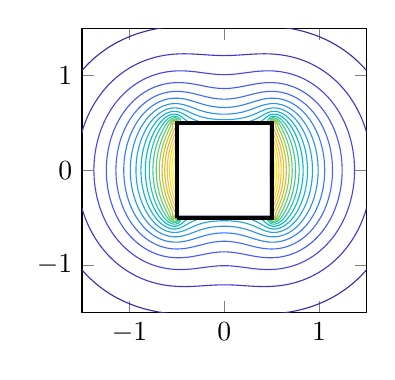
\begin{tikzpicture}

\begin{axis}[%
width=1.422in,
height=1.422in,
at={(0.406in,0.406in)},
scale only axis,
colormap={mymap}{[1pt] rgb(0pt)=(0.2422,0.1504,0.6603); rgb(1pt)=(0.25039,0.164995,0.707614); rgb(2pt)=(0.257771,0.181781,0.751138); rgb(3pt)=(0.264729,0.197757,0.795214); rgb(4pt)=(0.270648,0.214676,0.836371); rgb(5pt)=(0.275114,0.234238,0.870986); rgb(6pt)=(0.2783,0.255871,0.899071); rgb(7pt)=(0.280333,0.278233,0.9221); rgb(8pt)=(0.281338,0.300595,0.941376); rgb(9pt)=(0.281014,0.322757,0.957886); rgb(10pt)=(0.279467,0.344671,0.971676); rgb(11pt)=(0.275971,0.366681,0.982905); rgb(12pt)=(0.269914,0.3892,0.9906); rgb(13pt)=(0.260243,0.412329,0.995157); rgb(14pt)=(0.244033,0.435833,0.998833); rgb(15pt)=(0.220643,0.460257,0.997286); rgb(16pt)=(0.196333,0.484719,0.989152); rgb(17pt)=(0.183405,0.507371,0.979795); rgb(18pt)=(0.178643,0.528857,0.968157); rgb(19pt)=(0.176438,0.549905,0.952019); rgb(20pt)=(0.168743,0.570262,0.935871); rgb(21pt)=(0.154,0.5902,0.9218); rgb(22pt)=(0.146029,0.609119,0.907857); rgb(23pt)=(0.138024,0.627629,0.89729); rgb(24pt)=(0.124814,0.645929,0.888343); rgb(25pt)=(0.111252,0.6635,0.876314); rgb(26pt)=(0.0952095,0.679829,0.859781); rgb(27pt)=(0.0688714,0.694771,0.839357); rgb(28pt)=(0.0296667,0.708167,0.816333); rgb(29pt)=(0.00357143,0.720267,0.7917); rgb(30pt)=(0.00665714,0.731214,0.766014); rgb(31pt)=(0.0433286,0.741095,0.73941); rgb(32pt)=(0.0963952,0.75,0.712038); rgb(33pt)=(0.140771,0.7584,0.684157); rgb(34pt)=(0.1717,0.766962,0.655443); rgb(35pt)=(0.193767,0.775767,0.6251); rgb(36pt)=(0.216086,0.7843,0.5923); rgb(37pt)=(0.246957,0.791795,0.556743); rgb(38pt)=(0.290614,0.79729,0.518829); rgb(39pt)=(0.340643,0.8008,0.478857); rgb(40pt)=(0.3909,0.802871,0.435448); rgb(41pt)=(0.445629,0.802419,0.390919); rgb(42pt)=(0.5044,0.7993,0.348); rgb(43pt)=(0.561562,0.794233,0.304481); rgb(44pt)=(0.617395,0.787619,0.261238); rgb(45pt)=(0.671986,0.779271,0.2227); rgb(46pt)=(0.7242,0.769843,0.191029); rgb(47pt)=(0.773833,0.759805,0.16461); rgb(48pt)=(0.820314,0.749814,0.153529); rgb(49pt)=(0.863433,0.7406,0.159633); rgb(50pt)=(0.903543,0.733029,0.177414); rgb(51pt)=(0.939257,0.728786,0.209957); rgb(52pt)=(0.972757,0.729771,0.239443); rgb(53pt)=(0.995648,0.743371,0.237148); rgb(54pt)=(0.996986,0.765857,0.219943); rgb(55pt)=(0.995205,0.789252,0.202762); rgb(56pt)=(0.9892,0.813567,0.188533); rgb(57pt)=(0.978629,0.838629,0.176557); rgb(58pt)=(0.967648,0.8639,0.16429); rgb(59pt)=(0.96101,0.889019,0.153676); rgb(60pt)=(0.959671,0.913457,0.142257); rgb(61pt)=(0.962795,0.937338,0.12651); rgb(62pt)=(0.969114,0.960629,0.106362); rgb(63pt)=(0.9769,0.9839,0.0805)},
xmin=-1.5000,
xmax=1.5000,
ymin=-1.5000,
ymax=1.5000,
axis background/.style={fill=white}
]
\addplot[contour prepared, contour prepared format=matlab, contour/labels=false] table[row sep=crcr] {%
%
0.0476	549.0000\\
-1.8781	-0.0669\\
-1.8786	-0.0572\\
-1.8794	-0.0323\\
-1.8797	-0.0075\\
-1.8797	0.0174\\
-1.8792	0.0423\\
-1.8784	0.0672\\
-1.8781	0.0722\\
-1.8772	0.0920\\
-1.8757	0.1169\\
-1.8738	0.1418\\
-1.8715	0.1667\\
-1.8688	0.1915\\
-1.8656	0.2164\\
-1.8621	0.2413\\
-1.8580	0.2662\\
-1.8535	0.2910\\
-1.8532	0.2925\\
-1.8490	0.3159\\
-1.8440	0.3408\\
-1.8386	0.3657\\
-1.8326	0.3905\\
-1.8284	0.4068\\
-1.8263	0.4154\\
-1.8198	0.4403\\
-1.8128	0.4652\\
-1.8052	0.4900\\
-1.8035	0.4952\\
-1.7975	0.5149\\
-1.7893	0.5398\\
-1.7804	0.5647\\
-1.7786	0.5695\\
-1.7715	0.5896\\
-1.7619	0.6144\\
-1.7537	0.6344\\
-1.7518	0.6393\\
-1.7415	0.6642\\
-1.7304	0.6891\\
-1.7289	0.6925\\
-1.7192	0.7139\\
-1.7072	0.7388\\
-1.7040	0.7451\\
-1.6948	0.7637\\
-1.6817	0.7886\\
-1.6791	0.7933\\
-1.6682	0.8134\\
-1.6542	0.8377\\
-1.6539	0.8383\\
-1.6393	0.8632\\
-1.6294	0.8790\\
-1.6238	0.8881\\
-1.6076	0.9129\\
-1.6045	0.9175\\
-1.5907	0.9378\\
-1.5796	0.9535\\
-1.5730	0.9627\\
-1.5547	0.9872\\
-1.5544	0.9876\\
-1.5351	1.0124\\
-1.5299	1.0190\\
-1.5149	1.0373\\
-1.5050	1.0489\\
-1.4935	1.0622\\
-1.4801	1.0772\\
-1.4711	1.0871\\
-1.4552	1.1039\\
-1.4475	1.1119\\
-1.4303	1.1292\\
-1.4226	1.1368\\
-1.4055	1.1532\\
-1.3963	1.1617\\
-1.3806	1.1759\\
-1.3685	1.1866\\
-1.3557	1.1975\\
-1.3389	1.2114\\
-1.3308	1.2180\\
-1.3074	1.2363\\
-1.3060	1.2374\\
-1.2811	1.2560\\
-1.2739	1.2612\\
-1.2562	1.2737\\
-1.2378	1.2861\\
-1.2313	1.2904\\
-1.2065	1.3063\\
-1.1990	1.3109\\
-1.1816	1.3215\\
-1.1568	1.3358\\
-1.1567	1.3358\\
-1.1318	1.3497\\
-1.1106	1.3607\\
-1.1070	1.3626\\
-1.0821	1.3750\\
-1.0595	1.3856\\
-1.0572	1.3867\\
-1.0323	1.3979\\
-1.0075	1.4083\\
-1.0021	1.4104\\
-0.9826	1.4184\\
-0.9577	1.4278\\
-0.9363	1.4353\\
-0.9328	1.4366\\
-0.9080	1.4450\\
-0.8831	1.4529\\
-0.8582	1.4602\\
-0.8581	1.4602\\
-0.8333	1.4672\\
-0.8085	1.4737\\
-0.7836	1.4796\\
-0.7589	1.4851\\
-0.7587	1.4851\\
-0.7338	1.4904\\
-0.7090	1.4952\\
-0.6841	1.4995\\
-0.6592	1.5034\\
-0.6343	1.5070\\
-0.6110	1.5100\\
-0.6095	1.5101\\
-0.5846	1.5131\\
-0.5597	1.5157\\
-0.5348	1.5179\\
-0.5100	1.5198\\
-0.4851	1.5215\\
-0.4602	1.5228\\
-0.4353	1.5239\\
-0.4104	1.5248\\
-0.3856	1.5254\\
-0.3607	1.5258\\
-0.3358	1.5261\\
-0.3109	1.5262\\
-0.2861	1.5261\\
-0.2612	1.5260\\
-0.2363	1.5258\\
-0.2114	1.5255\\
-0.1866	1.5252\\
-0.1617	1.5248\\
-0.1368	1.5245\\
-0.1119	1.5242\\
-0.0871	1.5239\\
-0.0622	1.5237\\
-0.0373	1.5235\\
-0.0124	1.5235\\
0.0124	1.5235\\
0.0373	1.5235\\
0.0622	1.5237\\
0.0871	1.5239\\
0.1119	1.5242\\
0.1368	1.5245\\
0.1617	1.5248\\
0.1866	1.5252\\
0.2114	1.5255\\
0.2363	1.5258\\
0.2612	1.5260\\
0.2861	1.5261\\
0.3109	1.5262\\
0.3358	1.5261\\
0.3607	1.5258\\
0.3856	1.5254\\
0.4104	1.5248\\
0.4353	1.5239\\
0.4602	1.5228\\
0.4851	1.5215\\
0.5100	1.5198\\
0.5348	1.5179\\
0.5597	1.5157\\
0.5846	1.5131\\
0.6095	1.5101\\
0.6110	1.5100\\
0.6343	1.5070\\
0.6592	1.5034\\
0.6841	1.4995\\
0.7090	1.4952\\
0.7338	1.4904\\
0.7587	1.4851\\
0.7589	1.4851\\
0.7836	1.4796\\
0.8085	1.4737\\
0.8333	1.4672\\
0.8581	1.4602\\
0.8582	1.4602\\
0.8831	1.4529\\
0.9080	1.4450\\
0.9328	1.4366\\
0.9363	1.4353\\
0.9577	1.4278\\
0.9826	1.4184\\
1.0021	1.4104\\
1.0075	1.4083\\
1.0323	1.3979\\
1.0572	1.3867\\
1.0595	1.3856\\
1.0821	1.3750\\
1.1070	1.3626\\
1.1106	1.3607\\
1.1318	1.3497\\
1.1567	1.3358\\
1.1568	1.3358\\
1.1816	1.3215\\
1.1990	1.3109\\
1.2065	1.3063\\
1.2313	1.2904\\
1.2378	1.2861\\
1.2562	1.2737\\
1.2739	1.2612\\
1.2811	1.2560\\
1.3060	1.2374\\
1.3074	1.2363\\
1.3308	1.2180\\
1.3389	1.2114\\
1.3557	1.1975\\
1.3685	1.1866\\
1.3806	1.1759\\
1.3963	1.1617\\
1.4055	1.1532\\
1.4226	1.1368\\
1.4303	1.1292\\
1.4475	1.1119\\
1.4552	1.1039\\
1.4711	1.0871\\
1.4801	1.0772\\
1.4935	1.0622\\
1.5050	1.0489\\
1.5149	1.0373\\
1.5299	1.0190\\
1.5351	1.0124\\
1.5544	0.9876\\
1.5547	0.9872\\
1.5730	0.9627\\
1.5796	0.9535\\
1.5907	0.9378\\
1.6045	0.9175\\
1.6076	0.9129\\
1.6238	0.8881\\
1.6294	0.8790\\
1.6393	0.8632\\
1.6539	0.8383\\
1.6542	0.8377\\
1.6682	0.8134\\
1.6791	0.7933\\
1.6817	0.7886\\
1.6948	0.7637\\
1.7040	0.7451\\
1.7072	0.7388\\
1.7192	0.7139\\
1.7289	0.6925\\
1.7304	0.6891\\
1.7415	0.6642\\
1.7518	0.6393\\
1.7537	0.6344\\
1.7619	0.6144\\
1.7715	0.5896\\
1.7786	0.5695\\
1.7804	0.5647\\
1.7893	0.5398\\
1.7975	0.5149\\
1.8035	0.4952\\
1.8052	0.4900\\
1.8128	0.4652\\
1.8198	0.4403\\
1.8263	0.4154\\
1.8284	0.4068\\
1.8326	0.3905\\
1.8386	0.3657\\
1.8440	0.3408\\
1.8490	0.3159\\
1.8532	0.2925\\
1.8535	0.2910\\
1.8580	0.2662\\
1.8621	0.2413\\
1.8656	0.2164\\
1.8688	0.1915\\
1.8715	0.1667\\
1.8738	0.1418\\
1.8757	0.1169\\
1.8772	0.0920\\
1.8781	0.0722\\
1.8784	0.0672\\
1.8792	0.0423\\
1.8797	0.0174\\
1.8797	-0.0075\\
1.8794	-0.0323\\
1.8786	-0.0572\\
1.8781	-0.0669\\
1.8775	-0.0821\\
1.8760	-0.1070\\
1.8742	-0.1318\\
1.8720	-0.1567\\
1.8693	-0.1816\\
1.8663	-0.2065\\
1.8628	-0.2313\\
1.8589	-0.2562\\
1.8545	-0.2811\\
1.8532	-0.2874\\
1.8499	-0.3060\\
1.8451	-0.3308\\
1.8397	-0.3557\\
1.8338	-0.3806\\
1.8284	-0.4019\\
1.8275	-0.4055\\
1.8212	-0.4303\\
1.8142	-0.4552\\
1.8067	-0.4801\\
1.8035	-0.4902\\
1.7990	-0.5050\\
1.7910	-0.5299\\
1.7823	-0.5547\\
1.7786	-0.5645\\
1.7733	-0.5796\\
1.7639	-0.6045\\
1.7538	-0.6294\\
1.7537	-0.6295\\
1.7437	-0.6542\\
1.7327	-0.6791\\
1.7289	-0.6875\\
1.7215	-0.7040\\
1.7096	-0.7289\\
1.7040	-0.7401\\
1.6973	-0.7537\\
1.6844	-0.7786\\
1.6791	-0.7883\\
1.6710	-0.8035\\
1.6568	-0.8284\\
1.6542	-0.8328\\
1.6423	-0.8532\\
1.6294	-0.8740\\
1.6268	-0.8781\\
1.6109	-0.9030\\
1.6045	-0.9125\\
1.5942	-0.9279\\
1.5796	-0.9485\\
1.5766	-0.9527\\
1.5583	-0.9776\\
1.5547	-0.9822\\
1.5391	-1.0025\\
1.5299	-1.0140\\
1.5190	-1.0274\\
1.5050	-1.0439\\
1.4979	-1.0522\\
1.4801	-1.0722\\
1.4756	-1.0771\\
1.4552	-1.0989\\
1.4523	-1.1020\\
1.4303	-1.1242\\
1.4276	-1.1269\\
1.4055	-1.1482\\
1.4016	-1.1517\\
1.3806	-1.1709\\
1.3741	-1.1766\\
1.3557	-1.1925\\
1.3450	-1.2015\\
1.3308	-1.2130\\
1.3139	-1.2264\\
1.3060	-1.2325\\
1.2811	-1.2510\\
1.2807	-1.2512\\
1.2562	-1.2687\\
1.2453	-1.2761\\
1.2313	-1.2855\\
1.2070	-1.3010\\
1.2065	-1.3013\\
1.1816	-1.3166\\
1.1655	-1.3259\\
1.1567	-1.3309\\
1.1318	-1.3447\\
1.1202	-1.3507\\
1.1070	-1.3577\\
1.0821	-1.3700\\
1.0702	-1.3756\\
1.0572	-1.3818\\
1.0323	-1.3929\\
1.0142	-1.4005\\
1.0075	-1.4034\\
0.9826	-1.4134\\
0.9577	-1.4227\\
0.9503	-1.4254\\
0.9328	-1.4317\\
0.9080	-1.4401\\
0.8831	-1.4479\\
0.8750	-1.4502\\
0.8582	-1.4553\\
0.8333	-1.4622\\
0.8085	-1.4687\\
0.7836	-1.4746\\
0.7811	-1.4751\\
0.7587	-1.4802\\
0.7338	-1.4854\\
0.7090	-1.4902\\
0.6841	-1.4945\\
0.6592	-1.4984\\
0.6478	-1.5000\\
0.6343	-1.5020\\
0.6095	-1.5053\\
0.5846	-1.5082\\
0.5597	-1.5107\\
0.5348	-1.5130\\
0.5100	-1.5149\\
0.4851	-1.5165\\
0.4602	-1.5178\\
0.4353	-1.5189\\
0.4104	-1.5197\\
0.3856	-1.5204\\
0.3607	-1.5208\\
0.3358	-1.5210\\
0.3109	-1.5211\\
0.2861	-1.5211\\
0.2612	-1.5210\\
0.2363	-1.5208\\
0.2114	-1.5205\\
0.1866	-1.5201\\
0.1617	-1.5198\\
0.1368	-1.5195\\
0.1119	-1.5192\\
0.0871	-1.5189\\
0.0622	-1.5187\\
0.0373	-1.5185\\
0.0124	-1.5185\\
-0.0124	-1.5185\\
-0.0373	-1.5185\\
-0.0622	-1.5187\\
-0.0871	-1.5189\\
-0.1119	-1.5192\\
-0.1368	-1.5195\\
-0.1617	-1.5198\\
-0.1866	-1.5201\\
-0.2114	-1.5205\\
-0.2363	-1.5208\\
-0.2612	-1.5210\\
-0.2861	-1.5211\\
-0.3109	-1.5211\\
-0.3358	-1.5210\\
-0.3607	-1.5208\\
-0.3856	-1.5204\\
-0.4104	-1.5197\\
-0.4353	-1.5189\\
-0.4602	-1.5178\\
-0.4851	-1.5165\\
-0.5100	-1.5149\\
-0.5348	-1.5130\\
-0.5597	-1.5107\\
-0.5846	-1.5082\\
-0.6095	-1.5053\\
-0.6343	-1.5020\\
-0.6478	-1.5000\\
-0.6592	-1.4984\\
-0.6841	-1.4945\\
-0.7090	-1.4902\\
-0.7338	-1.4854\\
-0.7587	-1.4802\\
-0.7811	-1.4751\\
-0.7836	-1.4746\\
-0.8085	-1.4687\\
-0.8333	-1.4622\\
-0.8582	-1.4553\\
-0.8750	-1.4502\\
-0.8831	-1.4479\\
-0.9080	-1.4401\\
-0.9328	-1.4317\\
-0.9503	-1.4254\\
-0.9577	-1.4227\\
-0.9826	-1.4134\\
-1.0075	-1.4034\\
-1.0142	-1.4005\\
-1.0323	-1.3929\\
-1.0572	-1.3818\\
-1.0702	-1.3756\\
-1.0821	-1.3700\\
-1.1070	-1.3577\\
-1.1202	-1.3507\\
-1.1318	-1.3447\\
-1.1567	-1.3309\\
-1.1655	-1.3259\\
-1.1816	-1.3166\\
-1.2065	-1.3013\\
-1.2070	-1.3010\\
-1.2313	-1.2855\\
-1.2453	-1.2761\\
-1.2562	-1.2687\\
-1.2807	-1.2512\\
-1.2811	-1.2510\\
-1.3060	-1.2325\\
-1.3139	-1.2264\\
-1.3308	-1.2130\\
-1.3450	-1.2015\\
-1.3557	-1.1925\\
-1.3741	-1.1766\\
-1.3806	-1.1709\\
-1.4016	-1.1517\\
-1.4055	-1.1482\\
-1.4276	-1.1269\\
-1.4303	-1.1242\\
-1.4523	-1.1020\\
-1.4552	-1.0989\\
-1.4756	-1.0771\\
-1.4801	-1.0722\\
-1.4979	-1.0522\\
-1.5050	-1.0439\\
-1.5190	-1.0274\\
-1.5299	-1.0140\\
-1.5391	-1.0025\\
-1.5547	-0.9822\\
-1.5583	-0.9776\\
-1.5766	-0.9527\\
-1.5796	-0.9485\\
-1.5942	-0.9279\\
-1.6045	-0.9125\\
-1.6109	-0.9030\\
-1.6268	-0.8781\\
-1.6294	-0.8740\\
-1.6423	-0.8532\\
-1.6542	-0.8328\\
-1.6568	-0.8284\\
-1.6710	-0.8035\\
-1.6791	-0.7883\\
-1.6844	-0.7786\\
-1.6973	-0.7537\\
-1.7040	-0.7401\\
-1.7096	-0.7289\\
-1.7215	-0.7040\\
-1.7289	-0.6875\\
-1.7327	-0.6791\\
-1.7437	-0.6542\\
-1.7537	-0.6295\\
-1.7538	-0.6294\\
-1.7639	-0.6045\\
-1.7733	-0.5796\\
-1.7786	-0.5645\\
-1.7823	-0.5547\\
-1.7910	-0.5299\\
-1.7990	-0.5050\\
-1.8035	-0.4902\\
-1.8067	-0.4801\\
-1.8142	-0.4552\\
-1.8212	-0.4303\\
-1.8275	-0.4055\\
-1.8284	-0.4019\\
-1.8338	-0.3806\\
-1.8397	-0.3557\\
-1.8451	-0.3308\\
-1.8499	-0.3060\\
-1.8532	-0.2874\\
-1.8545	-0.2811\\
-1.8589	-0.2562\\
-1.8628	-0.2313\\
-1.8663	-0.2065\\
-1.8693	-0.1816\\
-1.8720	-0.1567\\
-1.8742	-0.1318\\
-1.8760	-0.1070\\
-1.8775	-0.0821\\
-1.8781	-0.0669\\
0.0476	161.0000\\
-0.4851	0.4923\\
-0.4866	0.4900\\
-0.4867	0.4652\\
-0.4866	0.4403\\
-0.4865	0.4154\\
-0.4865	0.3905\\
-0.4865	0.3657\\
-0.4865	0.3408\\
-0.4864	0.3159\\
-0.4864	0.2910\\
-0.4864	0.2662\\
-0.4864	0.2413\\
-0.4863	0.2164\\
-0.4863	0.1915\\
-0.4863	0.1667\\
-0.4863	0.1418\\
-0.4863	0.1169\\
-0.4863	0.0920\\
-0.4863	0.0672\\
-0.4863	0.0423\\
-0.4863	0.0174\\
-0.4863	-0.0075\\
-0.4863	-0.0323\\
-0.4863	-0.0572\\
-0.4863	-0.0821\\
-0.4863	-0.1070\\
-0.4863	-0.1318\\
-0.4863	-0.1567\\
-0.4863	-0.1816\\
-0.4863	-0.2065\\
-0.4863	-0.2313\\
-0.4864	-0.2562\\
-0.4864	-0.2811\\
-0.4864	-0.3060\\
-0.4864	-0.3308\\
-0.4865	-0.3557\\
-0.4865	-0.3806\\
-0.4865	-0.4055\\
-0.4866	-0.4303\\
-0.4867	-0.4552\\
-0.4870	-0.4801\\
-0.4851	-0.4828\\
-0.4602	-0.4823\\
-0.4353	-0.4824\\
-0.4104	-0.4825\\
-0.3856	-0.4826\\
-0.3607	-0.4826\\
-0.3358	-0.4827\\
-0.3109	-0.4827\\
-0.2861	-0.4828\\
-0.2612	-0.4828\\
-0.2363	-0.4829\\
-0.2114	-0.4829\\
-0.1866	-0.4829\\
-0.1617	-0.4830\\
-0.1368	-0.4830\\
-0.1119	-0.4830\\
-0.0871	-0.4830\\
-0.0622	-0.4830\\
-0.0373	-0.4830\\
-0.0124	-0.4830\\
0.0124	-0.4830\\
0.0373	-0.4830\\
0.0622	-0.4830\\
0.0871	-0.4830\\
0.1119	-0.4830\\
0.1368	-0.4830\\
0.1617	-0.4830\\
0.1866	-0.4829\\
0.2114	-0.4829\\
0.2363	-0.4829\\
0.2612	-0.4828\\
0.2861	-0.4828\\
0.3109	-0.4827\\
0.3358	-0.4827\\
0.3607	-0.4826\\
0.3856	-0.4826\\
0.4104	-0.4825\\
0.4353	-0.4824\\
0.4602	-0.4823\\
0.4851	-0.4828\\
0.4870	-0.4801\\
0.4867	-0.4552\\
0.4866	-0.4303\\
0.4865	-0.4055\\
0.4865	-0.3806\\
0.4865	-0.3557\\
0.4864	-0.3308\\
0.4864	-0.3060\\
0.4864	-0.2811\\
0.4864	-0.2562\\
0.4863	-0.2313\\
0.4863	-0.2065\\
0.4863	-0.1816\\
0.4863	-0.1567\\
0.4863	-0.1318\\
0.4863	-0.1070\\
0.4863	-0.0821\\
0.4863	-0.0572\\
0.4863	-0.0323\\
0.4863	-0.0075\\
0.4863	0.0174\\
0.4863	0.0423\\
0.4863	0.0672\\
0.4863	0.0920\\
0.4863	0.1169\\
0.4863	0.1418\\
0.4863	0.1667\\
0.4863	0.1915\\
0.4863	0.2164\\
0.4864	0.2413\\
0.4864	0.2662\\
0.4864	0.2910\\
0.4864	0.3159\\
0.4865	0.3408\\
0.4865	0.3657\\
0.4865	0.3905\\
0.4865	0.4154\\
0.4866	0.4403\\
0.4867	0.4652\\
0.4866	0.4900\\
0.4851	0.4923\\
0.4602	0.4923\\
0.4353	0.4924\\
0.4104	0.4924\\
0.3856	0.4925\\
0.3607	0.4926\\
0.3358	0.4927\\
0.3109	0.4927\\
0.2861	0.4928\\
0.2612	0.4928\\
0.2363	0.4928\\
0.2114	0.4929\\
0.1866	0.4929\\
0.1617	0.4929\\
0.1368	0.4930\\
0.1119	0.4930\\
0.0871	0.4930\\
0.0622	0.4930\\
0.0373	0.4930\\
0.0124	0.4930\\
-0.0124	0.4930\\
-0.0373	0.4930\\
-0.0622	0.4930\\
-0.0871	0.4930\\
-0.1119	0.4930\\
-0.1368	0.4930\\
-0.1617	0.4929\\
-0.1866	0.4929\\
-0.2114	0.4929\\
-0.2363	0.4928\\
-0.2612	0.4928\\
-0.2861	0.4928\\
-0.3109	0.4927\\
-0.3358	0.4927\\
-0.3607	0.4926\\
-0.3856	0.4925\\
-0.4104	0.4924\\
-0.4353	0.4924\\
-0.4602	0.4923\\
-0.4851	0.4923\\
0.0952	449.0000\\
-1.5547	-0.0869\\
-1.5550	-0.0821\\
-1.5563	-0.0572\\
-1.5571	-0.0323\\
-1.5575	-0.0075\\
-1.5575	0.0174\\
-1.5570	0.0423\\
-1.5561	0.0672\\
-1.5547	0.0920\\
-1.5547	0.0923\\
-1.5531	0.1169\\
-1.5509	0.1418\\
-1.5484	0.1667\\
-1.5454	0.1915\\
-1.5420	0.2164\\
-1.5380	0.2413\\
-1.5336	0.2662\\
-1.5299	0.2852\\
-1.5287	0.2910\\
-1.5236	0.3159\\
-1.5178	0.3408\\
-1.5116	0.3657\\
-1.5050	0.3896\\
-1.5047	0.3905\\
-1.4976	0.4154\\
-1.4899	0.4403\\
-1.4815	0.4652\\
-1.4801	0.4690\\
-1.4727	0.4900\\
-1.4633	0.5149\\
-1.4552	0.5349\\
-1.4533	0.5398\\
-1.4428	0.5647\\
-1.4314	0.5896\\
-1.4303	0.5918\\
-1.4197	0.6144\\
-1.4070	0.6393\\
-1.4055	0.6421\\
-1.3938	0.6642\\
-1.3806	0.6873\\
-1.3796	0.6891\\
-1.3649	0.7139\\
-1.3557	0.7284\\
-1.3492	0.7388\\
-1.3325	0.7637\\
-1.3308	0.7661\\
-1.3151	0.7886\\
-1.3060	0.8008\\
-1.2965	0.8134\\
-1.2811	0.8330\\
-1.2768	0.8383\\
-1.2562	0.8628\\
-1.2559	0.8632\\
-1.2338	0.8881\\
-1.2313	0.8908\\
-1.2103	0.9129\\
-1.2065	0.9168\\
-1.1852	0.9378\\
-1.1816	0.9413\\
-1.1583	0.9627\\
-1.1567	0.9641\\
-1.1318	0.9856\\
-1.1295	0.9876\\
-1.1070	1.0059\\
-1.0985	1.0124\\
-1.0821	1.0249\\
-1.0648	1.0373\\
-1.0572	1.0427\\
-1.0323	1.0594\\
-1.0279	1.0622\\
-1.0075	1.0752\\
-0.9873	1.0871\\
-0.9826	1.0898\\
-0.9577	1.1037\\
-0.9418	1.1119\\
-0.9328	1.1166\\
-0.9080	1.1287\\
-0.8900	1.1368\\
-0.8831	1.1400\\
-0.8582	1.1505\\
-0.8333	1.1601\\
-0.8290	1.1617\\
-0.8085	1.1692\\
-0.7836	1.1775\\
-0.7587	1.1850\\
-0.7530	1.1866\\
-0.7338	1.1920\\
-0.7090	1.1983\\
-0.6841	1.2040\\
-0.6592	1.2089\\
-0.6450	1.2114\\
-0.6343	1.2134\\
-0.6095	1.2174\\
-0.5846	1.2207\\
-0.5597	1.2235\\
-0.5348	1.2258\\
-0.5100	1.2276\\
-0.4851	1.2289\\
-0.4602	1.2297\\
-0.4353	1.2302\\
-0.4104	1.2302\\
-0.3856	1.2299\\
-0.3607	1.2293\\
-0.3358	1.2284\\
-0.3109	1.2272\\
-0.2861	1.2258\\
-0.2612	1.2243\\
-0.2363	1.2226\\
-0.2114	1.2209\\
-0.1866	1.2192\\
-0.1617	1.2176\\
-0.1368	1.2160\\
-0.1119	1.2146\\
-0.0871	1.2134\\
-0.0622	1.2125\\
-0.0373	1.2119\\
-0.0124	1.2116\\
0.0124	1.2116\\
0.0373	1.2119\\
0.0622	1.2125\\
0.0871	1.2134\\
0.1119	1.2146\\
0.1368	1.2160\\
0.1617	1.2176\\
0.1866	1.2192\\
0.2114	1.2209\\
0.2363	1.2226\\
0.2612	1.2243\\
0.2861	1.2258\\
0.3109	1.2272\\
0.3358	1.2284\\
0.3607	1.2293\\
0.3856	1.2299\\
0.4104	1.2302\\
0.4353	1.2302\\
0.4602	1.2297\\
0.4851	1.2289\\
0.5100	1.2276\\
0.5348	1.2258\\
0.5597	1.2235\\
0.5846	1.2207\\
0.6095	1.2174\\
0.6343	1.2134\\
0.6450	1.2114\\
0.6592	1.2089\\
0.6841	1.2040\\
0.7090	1.1983\\
0.7338	1.1920\\
0.7530	1.1866\\
0.7587	1.1850\\
0.7836	1.1775\\
0.8085	1.1692\\
0.8290	1.1617\\
0.8333	1.1601\\
0.8582	1.1505\\
0.8831	1.1400\\
0.8900	1.1368\\
0.9080	1.1287\\
0.9328	1.1166\\
0.9418	1.1119\\
0.9577	1.1037\\
0.9826	1.0898\\
0.9873	1.0871\\
1.0075	1.0752\\
1.0279	1.0622\\
1.0323	1.0594\\
1.0572	1.0427\\
1.0648	1.0373\\
1.0821	1.0249\\
1.0985	1.0124\\
1.1070	1.0059\\
1.1295	0.9876\\
1.1318	0.9856\\
1.1567	0.9641\\
1.1583	0.9627\\
1.1816	0.9413\\
1.1852	0.9378\\
1.2065	0.9168\\
1.2103	0.9129\\
1.2313	0.8908\\
1.2338	0.8881\\
1.2559	0.8632\\
1.2562	0.8628\\
1.2768	0.8383\\
1.2811	0.8330\\
1.2965	0.8134\\
1.3060	0.8008\\
1.3151	0.7886\\
1.3308	0.7661\\
1.3325	0.7637\\
1.3492	0.7388\\
1.3557	0.7284\\
1.3649	0.7139\\
1.3796	0.6891\\
1.3806	0.6873\\
1.3938	0.6642\\
1.4055	0.6421\\
1.4070	0.6393\\
1.4197	0.6144\\
1.4303	0.5918\\
1.4314	0.5896\\
1.4428	0.5647\\
1.4533	0.5398\\
1.4552	0.5349\\
1.4633	0.5149\\
1.4727	0.4900\\
1.4801	0.4690\\
1.4815	0.4652\\
1.4899	0.4403\\
1.4976	0.4154\\
1.5047	0.3905\\
1.5050	0.3896\\
1.5116	0.3657\\
1.5178	0.3408\\
1.5236	0.3159\\
1.5287	0.2910\\
1.5299	0.2852\\
1.5336	0.2662\\
1.5380	0.2413\\
1.5420	0.2164\\
1.5454	0.1915\\
1.5484	0.1667\\
1.5509	0.1418\\
1.5531	0.1169\\
1.5547	0.0923\\
1.5547	0.0920\\
1.5561	0.0672\\
1.5570	0.0423\\
1.5575	0.0174\\
1.5575	-0.0075\\
1.5571	-0.0323\\
1.5563	-0.0572\\
1.5550	-0.0821\\
1.5547	-0.0869\\
1.5534	-0.1070\\
1.5514	-0.1318\\
1.5489	-0.1567\\
1.5460	-0.1816\\
1.5427	-0.2065\\
1.5388	-0.2313\\
1.5345	-0.2562\\
1.5299	-0.2804\\
1.5297	-0.2811\\
1.5246	-0.3060\\
1.5190	-0.3308\\
1.5129	-0.3557\\
1.5061	-0.3806\\
1.5050	-0.3846\\
1.4991	-0.4055\\
1.4915	-0.4303\\
1.4832	-0.4552\\
1.4801	-0.4640\\
1.4745	-0.4801\\
1.4653	-0.5050\\
1.4553	-0.5299\\
1.4552	-0.5300\\
1.4449	-0.5547\\
1.4338	-0.5796\\
1.4303	-0.5868\\
1.4221	-0.6045\\
1.4096	-0.6294\\
1.4055	-0.6371\\
1.3965	-0.6542\\
1.3825	-0.6791\\
1.3806	-0.6824\\
1.3679	-0.7040\\
1.3557	-0.7234\\
1.3523	-0.7289\\
1.3360	-0.7537\\
1.3308	-0.7611\\
1.3187	-0.7786\\
1.3060	-0.7958\\
1.3003	-0.8035\\
1.2811	-0.8280\\
1.2808	-0.8284\\
1.2602	-0.8532\\
1.2562	-0.8579\\
1.2384	-0.8781\\
1.2313	-0.8858\\
1.2152	-0.9030\\
1.2065	-0.9119\\
1.1904	-0.9279\\
1.1816	-0.9363\\
1.1639	-0.9527\\
1.1567	-0.9592\\
1.1355	-0.9776\\
1.1318	-0.9807\\
1.1070	-1.0008\\
1.1049	-1.0025\\
1.0821	-1.0199\\
1.0717	-1.0274\\
1.0572	-1.0377\\
1.0356	-1.0522\\
1.0323	-1.0544\\
1.0075	-1.0702\\
0.9958	-1.0771\\
0.9826	-1.0849\\
0.9577	-1.0987\\
0.9514	-1.1020\\
0.9328	-1.1117\\
0.9080	-1.1237\\
0.9010	-1.1269\\
0.8831	-1.1350\\
0.8582	-1.1455\\
0.8421	-1.1517\\
0.8333	-1.1552\\
0.8085	-1.1643\\
0.7836	-1.1725\\
0.7699	-1.1766\\
0.7587	-1.1801\\
0.7338	-1.1871\\
0.7090	-1.1934\\
0.6841	-1.1989\\
0.6712	-1.2015\\
0.6592	-1.2040\\
0.6343	-1.2085\\
0.6095	-1.2124\\
0.5846	-1.2158\\
0.5597	-1.2185\\
0.5348	-1.2208\\
0.5100	-1.2225\\
0.4851	-1.2238\\
0.4602	-1.2247\\
0.4353	-1.2251\\
0.4104	-1.2252\\
0.3856	-1.2249\\
0.3607	-1.2242\\
0.3358	-1.2233\\
0.3109	-1.2222\\
0.2861	-1.2208\\
0.2612	-1.2193\\
0.2363	-1.2176\\
0.2114	-1.2160\\
0.1866	-1.2143\\
0.1617	-1.2126\\
0.1368	-1.2111\\
0.1119	-1.2097\\
0.0871	-1.2085\\
0.0622	-1.2076\\
0.0373	-1.2070\\
0.0124	-1.2067\\
-0.0124	-1.2067\\
-0.0373	-1.2070\\
-0.0622	-1.2076\\
-0.0871	-1.2085\\
-0.1119	-1.2097\\
-0.1368	-1.2111\\
-0.1617	-1.2126\\
-0.1866	-1.2143\\
-0.2114	-1.2160\\
-0.2363	-1.2176\\
-0.2612	-1.2193\\
-0.2861	-1.2208\\
-0.3109	-1.2222\\
-0.3358	-1.2233\\
-0.3607	-1.2242\\
-0.3856	-1.2249\\
-0.4104	-1.2252\\
-0.4353	-1.2251\\
-0.4602	-1.2247\\
-0.4851	-1.2238\\
-0.5100	-1.2225\\
-0.5348	-1.2208\\
-0.5597	-1.2185\\
-0.5846	-1.2158\\
-0.6095	-1.2124\\
-0.6343	-1.2085\\
-0.6592	-1.2040\\
-0.6712	-1.2015\\
-0.6841	-1.1989\\
-0.7090	-1.1934\\
-0.7338	-1.1871\\
-0.7587	-1.1801\\
-0.7699	-1.1766\\
-0.7836	-1.1725\\
-0.8085	-1.1643\\
-0.8333	-1.1552\\
-0.8421	-1.1517\\
-0.8582	-1.1455\\
-0.8831	-1.1350\\
-0.9010	-1.1269\\
-0.9080	-1.1237\\
-0.9328	-1.1117\\
-0.9514	-1.1020\\
-0.9577	-1.0987\\
-0.9826	-1.0849\\
-0.9958	-1.0771\\
-1.0075	-1.0702\\
-1.0323	-1.0544\\
-1.0356	-1.0522\\
-1.0572	-1.0377\\
-1.0717	-1.0274\\
-1.0821	-1.0199\\
-1.1049	-1.0025\\
-1.1070	-1.0008\\
-1.1318	-0.9807\\
-1.1355	-0.9776\\
-1.1567	-0.9592\\
-1.1639	-0.9527\\
-1.1816	-0.9363\\
-1.1904	-0.9279\\
-1.2065	-0.9119\\
-1.2152	-0.9030\\
-1.2313	-0.8858\\
-1.2384	-0.8781\\
-1.2562	-0.8579\\
-1.2602	-0.8532\\
-1.2808	-0.8284\\
-1.2811	-0.8280\\
-1.3003	-0.8035\\
-1.3060	-0.7958\\
-1.3187	-0.7786\\
-1.3308	-0.7611\\
-1.3360	-0.7537\\
-1.3523	-0.7289\\
-1.3557	-0.7234\\
-1.3679	-0.7040\\
-1.3806	-0.6824\\
-1.3825	-0.6791\\
-1.3965	-0.6542\\
-1.4055	-0.6371\\
-1.4096	-0.6294\\
-1.4221	-0.6045\\
-1.4303	-0.5868\\
-1.4338	-0.5796\\
-1.4449	-0.5547\\
-1.4552	-0.5300\\
-1.4553	-0.5299\\
-1.4653	-0.5050\\
-1.4745	-0.4801\\
-1.4801	-0.4640\\
-1.4832	-0.4552\\
-1.4915	-0.4303\\
-1.4991	-0.4055\\
-1.5050	-0.3846\\
-1.5061	-0.3806\\
-1.5129	-0.3557\\
-1.5190	-0.3308\\
-1.5246	-0.3060\\
-1.5297	-0.2811\\
-1.5299	-0.2804\\
-1.5345	-0.2562\\
-1.5388	-0.2313\\
-1.5427	-0.2065\\
-1.5460	-0.1816\\
-1.5489	-0.1567\\
-1.5514	-0.1318\\
-1.5534	-0.1070\\
-1.5547	-0.0869\\
0.0952	161.0000\\
-0.4851	0.4945\\
-0.4881	0.4900\\
-0.4883	0.4652\\
-0.4881	0.4403\\
-0.4880	0.4154\\
-0.4880	0.3905\\
-0.4879	0.3657\\
-0.4878	0.3408\\
-0.4878	0.3159\\
-0.4877	0.2910\\
-0.4877	0.2662\\
-0.4876	0.2413\\
-0.4876	0.2164\\
-0.4876	0.1915\\
-0.4875	0.1667\\
-0.4875	0.1418\\
-0.4875	0.1169\\
-0.4875	0.0920\\
-0.4875	0.0672\\
-0.4874	0.0423\\
-0.4874	0.0174\\
-0.4874	-0.0075\\
-0.4874	-0.0323\\
-0.4875	-0.0572\\
-0.4875	-0.0821\\
-0.4875	-0.1070\\
-0.4875	-0.1318\\
-0.4875	-0.1567\\
-0.4876	-0.1816\\
-0.4876	-0.2065\\
-0.4876	-0.2313\\
-0.4877	-0.2562\\
-0.4877	-0.2811\\
-0.4878	-0.3060\\
-0.4878	-0.3308\\
-0.4879	-0.3557\\
-0.4879	-0.3806\\
-0.4880	-0.4055\\
-0.4881	-0.4303\\
-0.4882	-0.4552\\
-0.4889	-0.4801\\
-0.4851	-0.4855\\
-0.4602	-0.4846\\
-0.4353	-0.4847\\
-0.4104	-0.4849\\
-0.3856	-0.4850\\
-0.3607	-0.4852\\
-0.3358	-0.4853\\
-0.3109	-0.4854\\
-0.2861	-0.4855\\
-0.2612	-0.4856\\
-0.2363	-0.4856\\
-0.2114	-0.4857\\
-0.1866	-0.4858\\
-0.1617	-0.4858\\
-0.1368	-0.4858\\
-0.1119	-0.4859\\
-0.0871	-0.4859\\
-0.0622	-0.4859\\
-0.0373	-0.4859\\
-0.0124	-0.4859\\
0.0124	-0.4859\\
0.0373	-0.4859\\
0.0622	-0.4859\\
0.0871	-0.4859\\
0.1119	-0.4859\\
0.1368	-0.4858\\
0.1617	-0.4858\\
0.1866	-0.4858\\
0.2114	-0.4857\\
0.2363	-0.4856\\
0.2612	-0.4856\\
0.2861	-0.4855\\
0.3109	-0.4854\\
0.3358	-0.4853\\
0.3607	-0.4852\\
0.3856	-0.4850\\
0.4104	-0.4849\\
0.4353	-0.4847\\
0.4602	-0.4846\\
0.4851	-0.4855\\
0.4889	-0.4801\\
0.4882	-0.4552\\
0.4881	-0.4303\\
0.4880	-0.4055\\
0.4879	-0.3806\\
0.4879	-0.3557\\
0.4878	-0.3308\\
0.4878	-0.3060\\
0.4877	-0.2811\\
0.4877	-0.2562\\
0.4876	-0.2313\\
0.4876	-0.2065\\
0.4876	-0.1816\\
0.4875	-0.1567\\
0.4875	-0.1318\\
0.4875	-0.1070\\
0.4875	-0.0821\\
0.4875	-0.0572\\
0.4874	-0.0323\\
0.4874	-0.0075\\
0.4874	0.0174\\
0.4874	0.0423\\
0.4875	0.0672\\
0.4875	0.0920\\
0.4875	0.1169\\
0.4875	0.1418\\
0.4875	0.1667\\
0.4876	0.1915\\
0.4876	0.2164\\
0.4876	0.2413\\
0.4877	0.2662\\
0.4877	0.2910\\
0.4878	0.3159\\
0.4878	0.3408\\
0.4879	0.3657\\
0.4880	0.3905\\
0.4880	0.4154\\
0.4881	0.4403\\
0.4883	0.4652\\
0.4881	0.4900\\
0.4851	0.4945\\
0.4602	0.4946\\
0.4353	0.4947\\
0.4104	0.4948\\
0.3856	0.4950\\
0.3607	0.4952\\
0.3358	0.4953\\
0.3109	0.4954\\
0.2861	0.4955\\
0.2612	0.4956\\
0.2363	0.4957\\
0.2114	0.4957\\
0.1866	0.4958\\
0.1617	0.4958\\
0.1368	0.4959\\
0.1119	0.4959\\
0.0871	0.4959\\
0.0622	0.4959\\
0.0373	0.4960\\
0.0124	0.4960\\
-0.0124	0.4960\\
-0.0373	0.4960\\
-0.0622	0.4959\\
-0.0871	0.4959\\
-0.1119	0.4959\\
-0.1368	0.4959\\
-0.1617	0.4958\\
-0.1866	0.4958\\
-0.2114	0.4957\\
-0.2363	0.4957\\
-0.2612	0.4956\\
-0.2861	0.4955\\
-0.3109	0.4954\\
-0.3358	0.4953\\
-0.3607	0.4952\\
-0.3856	0.4950\\
-0.4104	0.4948\\
-0.4353	0.4947\\
-0.4602	0.4946\\
-0.4851	0.4945\\
0.1429	395.0000\\
-1.3557	-0.2160\\
-1.3574	-0.2065\\
-1.3614	-0.1816\\
-1.3648	-0.1567\\
-1.3677	-0.1318\\
-1.3701	-0.1070\\
-1.3720	-0.0821\\
-1.3733	-0.0572\\
-1.3742	-0.0323\\
-1.3747	-0.0075\\
-1.3746	0.0174\\
-1.3741	0.0423\\
-1.3731	0.0672\\
-1.3716	0.0920\\
-1.3696	0.1169\\
-1.3672	0.1418\\
-1.3642	0.1667\\
-1.3606	0.1915\\
-1.3566	0.2164\\
-1.3557	0.2211\\
-1.3521	0.2413\\
-1.3472	0.2662\\
-1.3416	0.2910\\
-1.3354	0.3159\\
-1.3308	0.3327\\
-1.3287	0.3408\\
-1.3215	0.3657\\
-1.3137	0.3905\\
-1.3060	0.4128\\
-1.3051	0.4154\\
-1.2961	0.4403\\
-1.2863	0.4652\\
-1.2811	0.4774\\
-1.2758	0.4900\\
-1.2647	0.5149\\
-1.2562	0.5325\\
-1.2527	0.5398\\
-1.2401	0.5647\\
-1.2313	0.5806\\
-1.2265	0.5896\\
-1.2120	0.6144\\
-1.2065	0.6234\\
-1.1967	0.6393\\
-1.1816	0.6621\\
-1.1802	0.6642\\
-1.1628	0.6891\\
-1.1567	0.6972\\
-1.1441	0.7139\\
-1.1318	0.7293\\
-1.1241	0.7388\\
-1.1070	0.7588\\
-1.1027	0.7637\\
-1.0821	0.7860\\
-1.0797	0.7886\\
-1.0572	0.8112\\
-1.0549	0.8134\\
-1.0323	0.8345\\
-1.0280	0.8383\\
-1.0075	0.8561\\
-0.9988	0.8632\\
-0.9826	0.8762\\
-0.9668	0.8881\\
-0.9577	0.8947\\
-0.9328	0.9119\\
-0.9312	0.9129\\
-0.9080	0.9279\\
-0.8913	0.9378\\
-0.8831	0.9426\\
-0.8582	0.9563\\
-0.8454	0.9627\\
-0.8333	0.9688\\
-0.8085	0.9803\\
-0.7910	0.9876\\
-0.7836	0.9907\\
-0.7587	1.0003\\
-0.7338	1.0088\\
-0.7221	1.0124\\
-0.7090	1.0166\\
-0.6841	1.0235\\
-0.6592	1.0295\\
-0.6343	1.0346\\
-0.6187	1.0373\\
-0.6095	1.0390\\
-0.5846	1.0427\\
-0.5597	1.0457\\
-0.5348	1.0479\\
-0.5100	1.0495\\
-0.4851	1.0504\\
-0.4602	1.0506\\
-0.4353	1.0502\\
-0.4104	1.0493\\
-0.3856	1.0479\\
-0.3607	1.0460\\
-0.3358	1.0436\\
-0.3109	1.0409\\
-0.2861	1.0379\\
-0.2816	1.0373\\
-0.2612	1.0348\\
-0.2363	1.0315\\
-0.2114	1.0281\\
-0.1866	1.0248\\
-0.1617	1.0216\\
-0.1368	1.0186\\
-0.1119	1.0160\\
-0.0871	1.0137\\
-0.0694	1.0124\\
-0.0622	1.0119\\
-0.0373	1.0108\\
-0.0124	1.0102\\
0.0124	1.0102\\
0.0373	1.0108\\
0.0622	1.0119\\
0.0694	1.0124\\
0.0871	1.0137\\
0.1119	1.0160\\
0.1368	1.0186\\
0.1617	1.0216\\
0.1866	1.0248\\
0.2114	1.0281\\
0.2363	1.0315\\
0.2612	1.0348\\
0.2816	1.0373\\
0.2861	1.0379\\
0.3109	1.0409\\
0.3358	1.0436\\
0.3607	1.0460\\
0.3856	1.0479\\
0.4104	1.0493\\
0.4353	1.0502\\
0.4602	1.0506\\
0.4851	1.0504\\
0.5100	1.0495\\
0.5348	1.0479\\
0.5597	1.0457\\
0.5846	1.0427\\
0.6095	1.0390\\
0.6187	1.0373\\
0.6343	1.0346\\
0.6592	1.0295\\
0.6841	1.0235\\
0.7090	1.0166\\
0.7221	1.0124\\
0.7338	1.0088\\
0.7587	1.0003\\
0.7836	0.9907\\
0.7910	0.9876\\
0.8085	0.9803\\
0.8333	0.9688\\
0.8454	0.9627\\
0.8582	0.9563\\
0.8831	0.9426\\
0.8913	0.9378\\
0.9080	0.9279\\
0.9312	0.9129\\
0.9328	0.9119\\
0.9577	0.8947\\
0.9668	0.8881\\
0.9826	0.8762\\
0.9988	0.8632\\
1.0075	0.8561\\
1.0280	0.8383\\
1.0323	0.8345\\
1.0549	0.8134\\
1.0572	0.8112\\
1.0797	0.7886\\
1.0821	0.7860\\
1.1027	0.7637\\
1.1070	0.7588\\
1.1241	0.7388\\
1.1318	0.7293\\
1.1441	0.7139\\
1.1567	0.6972\\
1.1628	0.6891\\
1.1802	0.6642\\
1.1816	0.6621\\
1.1967	0.6393\\
1.2065	0.6234\\
1.2120	0.6144\\
1.2265	0.5896\\
1.2313	0.5806\\
1.2401	0.5647\\
1.2527	0.5398\\
1.2562	0.5325\\
1.2647	0.5149\\
1.2758	0.4900\\
1.2811	0.4774\\
1.2863	0.4652\\
1.2961	0.4403\\
1.3051	0.4154\\
1.3060	0.4128\\
1.3137	0.3905\\
1.3215	0.3657\\
1.3287	0.3408\\
1.3308	0.3327\\
1.3354	0.3159\\
1.3416	0.2910\\
1.3472	0.2662\\
1.3521	0.2413\\
1.3557	0.2211\\
1.3566	0.2164\\
1.3606	0.1915\\
1.3642	0.1667\\
1.3672	0.1418\\
1.3696	0.1169\\
1.3716	0.0920\\
1.3731	0.0672\\
1.3741	0.0423\\
1.3746	0.0174\\
1.3747	-0.0075\\
1.3742	-0.0323\\
1.3733	-0.0572\\
1.3720	-0.0821\\
1.3701	-0.1070\\
1.3677	-0.1318\\
1.3648	-0.1567\\
1.3614	-0.1816\\
1.3574	-0.2065\\
1.3557	-0.2160\\
1.3531	-0.2313\\
1.3482	-0.2562\\
1.3428	-0.2811\\
1.3367	-0.3060\\
1.3308	-0.3278\\
1.3301	-0.3308\\
1.3230	-0.3557\\
1.3153	-0.3806\\
1.3068	-0.4055\\
1.3060	-0.4079\\
1.2980	-0.4303\\
1.2883	-0.4552\\
1.2811	-0.4725\\
1.2780	-0.4801\\
1.2670	-0.5050\\
1.2562	-0.5275\\
1.2551	-0.5299\\
1.2427	-0.5547\\
1.2313	-0.5756\\
1.2292	-0.5796\\
1.2150	-0.6045\\
1.2065	-0.6185\\
1.1998	-0.6294\\
1.1836	-0.6542\\
1.1816	-0.6571\\
1.1664	-0.6791\\
1.1567	-0.6922\\
1.1479	-0.7040\\
1.1318	-0.7243\\
1.1282	-0.7289\\
1.1070	-0.7537\\
1.1070	-0.7538\\
1.0844	-0.7786\\
1.0821	-0.7810\\
1.0600	-0.8035\\
1.0572	-0.8062\\
1.0336	-0.8284\\
1.0323	-0.8295\\
1.0075	-0.8511\\
1.0049	-0.8532\\
0.9826	-0.8712\\
0.9734	-0.8781\\
0.9577	-0.8898\\
0.9387	-0.9030\\
0.9328	-0.9070\\
0.9080	-0.9229\\
0.8997	-0.9279\\
0.8831	-0.9377\\
0.8582	-0.9512\\
0.8552	-0.9527\\
0.8333	-0.9638\\
0.8085	-0.9752\\
0.8028	-0.9776\\
0.7836	-0.9858\\
0.7587	-0.9953\\
0.7376	-1.0025\\
0.7338	-1.0038\\
0.7090	-1.0117\\
0.6841	-1.0185\\
0.6592	-1.0244\\
0.6449	-1.0274\\
0.6343	-1.0296\\
0.6095	-1.0341\\
0.5846	-1.0378\\
0.5597	-1.0408\\
0.5348	-1.0430\\
0.5100	-1.0445\\
0.4851	-1.0453\\
0.4602	-1.0456\\
0.4353	-1.0452\\
0.4104	-1.0443\\
0.3856	-1.0429\\
0.3607	-1.0410\\
0.3358	-1.0387\\
0.3109	-1.0360\\
0.2861	-1.0330\\
0.2612	-1.0298\\
0.2435	-1.0274\\
0.2363	-1.0264\\
0.2114	-1.0231\\
0.1866	-1.0198\\
0.1617	-1.0167\\
0.1368	-1.0137\\
0.1119	-1.0111\\
0.0871	-1.0088\\
0.0622	-1.0070\\
0.0373	-1.0058\\
0.0124	-1.0052\\
-0.0124	-1.0052\\
-0.0373	-1.0058\\
-0.0622	-1.0070\\
-0.0871	-1.0088\\
-0.1119	-1.0111\\
-0.1368	-1.0137\\
-0.1617	-1.0167\\
-0.1866	-1.0198\\
-0.2114	-1.0231\\
-0.2363	-1.0264\\
-0.2435	-1.0274\\
-0.2612	-1.0298\\
-0.2861	-1.0330\\
-0.3109	-1.0360\\
-0.3358	-1.0387\\
-0.3607	-1.0410\\
-0.3856	-1.0429\\
-0.4104	-1.0443\\
-0.4353	-1.0452\\
-0.4602	-1.0456\\
-0.4851	-1.0453\\
-0.5100	-1.0445\\
-0.5348	-1.0430\\
-0.5597	-1.0408\\
-0.5846	-1.0378\\
-0.6095	-1.0341\\
-0.6343	-1.0296\\
-0.6449	-1.0274\\
-0.6592	-1.0244\\
-0.6841	-1.0185\\
-0.7090	-1.0117\\
-0.7338	-1.0038\\
-0.7376	-1.0025\\
-0.7587	-0.9953\\
-0.7836	-0.9858\\
-0.8028	-0.9776\\
-0.8085	-0.9752\\
-0.8333	-0.9638\\
-0.8552	-0.9527\\
-0.8582	-0.9512\\
-0.8831	-0.9377\\
-0.8997	-0.9279\\
-0.9080	-0.9229\\
-0.9328	-0.9070\\
-0.9387	-0.9030\\
-0.9577	-0.8898\\
-0.9734	-0.8781\\
-0.9826	-0.8712\\
-1.0049	-0.8532\\
-1.0075	-0.8511\\
-1.0323	-0.8295\\
-1.0336	-0.8284\\
-1.0572	-0.8062\\
-1.0600	-0.8035\\
-1.0821	-0.7810\\
-1.0844	-0.7786\\
-1.1070	-0.7538\\
-1.1070	-0.7537\\
-1.1282	-0.7289\\
-1.1318	-0.7243\\
-1.1479	-0.7040\\
-1.1567	-0.6922\\
-1.1664	-0.6791\\
-1.1816	-0.6571\\
-1.1836	-0.6542\\
-1.1998	-0.6294\\
-1.2065	-0.6185\\
-1.2150	-0.6045\\
-1.2292	-0.5796\\
-1.2313	-0.5756\\
-1.2427	-0.5547\\
-1.2551	-0.5299\\
-1.2562	-0.5275\\
-1.2670	-0.5050\\
-1.2780	-0.4801\\
-1.2811	-0.4725\\
-1.2883	-0.4552\\
-1.2980	-0.4303\\
-1.3060	-0.4079\\
-1.3068	-0.4055\\
-1.3153	-0.3806\\
-1.3230	-0.3557\\
-1.3301	-0.3308\\
-1.3308	-0.3278\\
-1.3367	-0.3060\\
-1.3428	-0.2811\\
-1.3482	-0.2562\\
-1.3531	-0.2313\\
-1.3557	-0.2160\\
0.1429	161.0000\\
-0.4851	0.4967\\
-0.4897	0.4900\\
-0.4899	0.4652\\
-0.4896	0.4403\\
-0.4895	0.4154\\
-0.4894	0.3905\\
-0.4893	0.3657\\
-0.4892	0.3408\\
-0.4891	0.3159\\
-0.4890	0.2910\\
-0.4890	0.2662\\
-0.4889	0.2413\\
-0.4889	0.2164\\
-0.4888	0.1915\\
-0.4888	0.1667\\
-0.4887	0.1418\\
-0.4887	0.1169\\
-0.4887	0.0920\\
-0.4886	0.0672\\
-0.4886	0.0423\\
-0.4886	0.0174\\
-0.4886	-0.0075\\
-0.4886	-0.0323\\
-0.4886	-0.0572\\
-0.4887	-0.0821\\
-0.4887	-0.1070\\
-0.4887	-0.1318\\
-0.4887	-0.1567\\
-0.4888	-0.1816\\
-0.4888	-0.2065\\
-0.4889	-0.2313\\
-0.4890	-0.2562\\
-0.4890	-0.2811\\
-0.4891	-0.3060\\
-0.4892	-0.3308\\
-0.4893	-0.3557\\
-0.4894	-0.3806\\
-0.4895	-0.4055\\
-0.4896	-0.4303\\
-0.4898	-0.4552\\
-0.4908	-0.4801\\
-0.4851	-0.4882\\
-0.4602	-0.4868\\
-0.4353	-0.4870\\
-0.4104	-0.4872\\
-0.3856	-0.4875\\
-0.3607	-0.4877\\
-0.3358	-0.4879\\
-0.3109	-0.4880\\
-0.2861	-0.4882\\
-0.2612	-0.4883\\
-0.2363	-0.4884\\
-0.2114	-0.4885\\
-0.1866	-0.4886\\
-0.1617	-0.4887\\
-0.1368	-0.4887\\
-0.1119	-0.4888\\
-0.0871	-0.4888\\
-0.0622	-0.4888\\
-0.0373	-0.4889\\
-0.0124	-0.4889\\
0.0124	-0.4889\\
0.0373	-0.4889\\
0.0622	-0.4888\\
0.0871	-0.4888\\
0.1119	-0.4888\\
0.1368	-0.4887\\
0.1617	-0.4887\\
0.1866	-0.4886\\
0.2114	-0.4885\\
0.2363	-0.4884\\
0.2612	-0.4883\\
0.2861	-0.4882\\
0.3109	-0.4880\\
0.3358	-0.4879\\
0.3607	-0.4877\\
0.3856	-0.4875\\
0.4104	-0.4872\\
0.4353	-0.4870\\
0.4602	-0.4868\\
0.4851	-0.4882\\
0.4908	-0.4801\\
0.4898	-0.4552\\
0.4896	-0.4303\\
0.4895	-0.4055\\
0.4894	-0.3806\\
0.4893	-0.3557\\
0.4892	-0.3308\\
0.4891	-0.3060\\
0.4890	-0.2811\\
0.4890	-0.2562\\
0.4889	-0.2313\\
0.4888	-0.2065\\
0.4888	-0.1816\\
0.4887	-0.1567\\
0.4887	-0.1318\\
0.4887	-0.1070\\
0.4887	-0.0821\\
0.4886	-0.0572\\
0.4886	-0.0323\\
0.4886	-0.0075\\
0.4886	0.0174\\
0.4886	0.0423\\
0.4886	0.0672\\
0.4887	0.0920\\
0.4887	0.1169\\
0.4887	0.1418\\
0.4888	0.1667\\
0.4888	0.1915\\
0.4889	0.2164\\
0.4889	0.2413\\
0.4890	0.2662\\
0.4890	0.2910\\
0.4891	0.3159\\
0.4892	0.3408\\
0.4893	0.3657\\
0.4894	0.3905\\
0.4895	0.4154\\
0.4896	0.4403\\
0.4899	0.4652\\
0.4897	0.4900\\
0.4851	0.4967\\
0.4602	0.4968\\
0.4353	0.4970\\
0.4104	0.4972\\
0.3856	0.4975\\
0.3607	0.4977\\
0.3358	0.4979\\
0.3109	0.4981\\
0.2861	0.4982\\
0.2612	0.4983\\
0.2363	0.4985\\
0.2114	0.4986\\
0.1866	0.4986\\
0.1617	0.4987\\
0.1368	0.4988\\
0.1119	0.4988\\
0.0871	0.4989\\
0.0622	0.4989\\
0.0373	0.4989\\
0.0124	0.4989\\
-0.0124	0.4989\\
-0.0373	0.4989\\
-0.0622	0.4989\\
-0.0871	0.4989\\
-0.1119	0.4988\\
-0.1368	0.4988\\
-0.1617	0.4987\\
-0.1866	0.4986\\
-0.2114	0.4986\\
-0.2363	0.4985\\
-0.2612	0.4983\\
-0.2861	0.4982\\
-0.3109	0.4981\\
-0.3358	0.4979\\
-0.3607	0.4977\\
-0.3856	0.4975\\
-0.4104	0.4972\\
-0.4353	0.4970\\
-0.4602	0.4968\\
-0.4851	0.4967\\
0.1905	357.0000\\
-1.2313	-0.1667\\
-1.2329	-0.1567\\
-1.2361	-0.1318\\
-1.2387	-0.1070\\
-1.2408	-0.0821\\
-1.2424	-0.0572\\
-1.2434	-0.0323\\
-1.2439	-0.0075\\
-1.2438	0.0174\\
-1.2432	0.0423\\
-1.2421	0.0672\\
-1.2405	0.0920\\
-1.2382	0.1169\\
-1.2355	0.1418\\
-1.2321	0.1667\\
-1.2313	0.1718\\
-1.2284	0.1915\\
-1.2241	0.2164\\
-1.2191	0.2413\\
-1.2135	0.2662\\
-1.2073	0.2910\\
-1.2065	0.2939\\
-1.2006	0.3159\\
-1.1932	0.3408\\
-1.1850	0.3657\\
-1.1816	0.3753\\
-1.1763	0.3905\\
-1.1668	0.4154\\
-1.1567	0.4396\\
-1.1564	0.4403\\
-1.1456	0.4652\\
-1.1336	0.4900\\
-1.1318	0.4935\\
-1.1210	0.5149\\
-1.1071	0.5398\\
-1.1070	0.5401\\
-1.0926	0.5647\\
-1.0821	0.5812\\
-1.0767	0.5896\\
-1.0597	0.6144\\
-1.0572	0.6179\\
-1.0415	0.6393\\
-1.0323	0.6510\\
-1.0218	0.6642\\
-1.0075	0.6810\\
-1.0004	0.6891\\
-0.9826	0.7083\\
-0.9772	0.7139\\
-0.9577	0.7333\\
-0.9519	0.7388\\
-0.9328	0.7561\\
-0.9240	0.7637\\
-0.9080	0.7770\\
-0.8931	0.7886\\
-0.8831	0.7961\\
-0.8582	0.8134\\
-0.8582	0.8134\\
-0.8333	0.8294\\
-0.8181	0.8383\\
-0.8085	0.8439\\
-0.7836	0.8570\\
-0.7704	0.8632\\
-0.7587	0.8688\\
-0.7338	0.8794\\
-0.7103	0.8881\\
-0.7090	0.8886\\
-0.6841	0.8970\\
-0.6592	0.9041\\
-0.6343	0.9101\\
-0.6201	0.9129\\
-0.6095	0.9151\\
-0.5846	0.9193\\
-0.5597	0.9225\\
-0.5348	0.9247\\
-0.5100	0.9259\\
-0.4851	0.9264\\
-0.4602	0.9260\\
-0.4353	0.9248\\
-0.4104	0.9229\\
-0.3856	0.9202\\
-0.3607	0.9170\\
-0.3358	0.9131\\
-0.3348	0.9129\\
-0.3109	0.9090\\
-0.2861	0.9045\\
-0.2612	0.8996\\
-0.2363	0.8946\\
-0.2114	0.8896\\
-0.2039	0.8881\\
-0.1866	0.8847\\
-0.1617	0.8802\\
-0.1368	0.8760\\
-0.1119	0.8723\\
-0.0871	0.8691\\
-0.0622	0.8667\\
-0.0373	0.8650\\
-0.0124	0.8641\\
0.0124	0.8641\\
0.0373	0.8650\\
0.0622	0.8667\\
0.0871	0.8691\\
0.1119	0.8723\\
0.1368	0.8760\\
0.1617	0.8802\\
0.1866	0.8847\\
0.2039	0.8881\\
0.2114	0.8896\\
0.2363	0.8946\\
0.2612	0.8996\\
0.2861	0.9045\\
0.3109	0.9090\\
0.3348	0.9129\\
0.3358	0.9131\\
0.3607	0.9170\\
0.3856	0.9202\\
0.4104	0.9229\\
0.4353	0.9248\\
0.4602	0.9260\\
0.4851	0.9264\\
0.5100	0.9259\\
0.5348	0.9247\\
0.5597	0.9225\\
0.5846	0.9193\\
0.6095	0.9151\\
0.6201	0.9129\\
0.6343	0.9101\\
0.6592	0.9041\\
0.6841	0.8970\\
0.7090	0.8886\\
0.7103	0.8881\\
0.7338	0.8794\\
0.7587	0.8688\\
0.7704	0.8632\\
0.7836	0.8570\\
0.8085	0.8439\\
0.8181	0.8383\\
0.8333	0.8294\\
0.8582	0.8134\\
0.8582	0.8134\\
0.8831	0.7961\\
0.8931	0.7886\\
0.9080	0.7770\\
0.9240	0.7637\\
0.9328	0.7561\\
0.9519	0.7388\\
0.9577	0.7333\\
0.9772	0.7139\\
0.9826	0.7083\\
1.0004	0.6891\\
1.0075	0.6810\\
1.0218	0.6642\\
1.0323	0.6510\\
1.0415	0.6393\\
1.0572	0.6179\\
1.0597	0.6144\\
1.0767	0.5896\\
1.0821	0.5812\\
1.0926	0.5647\\
1.1070	0.5401\\
1.1071	0.5398\\
1.1210	0.5149\\
1.1318	0.4935\\
1.1336	0.4900\\
1.1456	0.4652\\
1.1564	0.4403\\
1.1567	0.4396\\
1.1668	0.4154\\
1.1763	0.3905\\
1.1816	0.3753\\
1.1850	0.3657\\
1.1932	0.3408\\
1.2006	0.3159\\
1.2065	0.2939\\
1.2073	0.2910\\
1.2135	0.2662\\
1.2191	0.2413\\
1.2241	0.2164\\
1.2284	0.1915\\
1.2313	0.1718\\
1.2321	0.1667\\
1.2355	0.1418\\
1.2382	0.1169\\
1.2405	0.0920\\
1.2421	0.0672\\
1.2432	0.0423\\
1.2438	0.0174\\
1.2439	-0.0075\\
1.2434	-0.0323\\
1.2424	-0.0572\\
1.2408	-0.0821\\
1.2387	-0.1070\\
1.2361	-0.1318\\
1.2329	-0.1567\\
1.2313	-0.1667\\
1.2292	-0.1816\\
1.2250	-0.2065\\
1.2202	-0.2313\\
1.2147	-0.2562\\
1.2086	-0.2811\\
1.2065	-0.2888\\
1.2020	-0.3060\\
1.1947	-0.3308\\
1.1867	-0.3557\\
1.1816	-0.3703\\
1.1781	-0.3806\\
1.1688	-0.4055\\
1.1586	-0.4303\\
1.1567	-0.4346\\
1.1478	-0.4552\\
1.1361	-0.4801\\
1.1318	-0.4885\\
1.1236	-0.5050\\
1.1100	-0.5299\\
1.1070	-0.5351\\
1.0956	-0.5547\\
1.0821	-0.5762\\
1.0799	-0.5796\\
1.0633	-0.6045\\
1.0572	-0.6129\\
1.0453	-0.6294\\
1.0323	-0.6460\\
1.0259	-0.6542\\
1.0075	-0.6760\\
1.0048	-0.6791\\
0.9826	-0.7033\\
0.9820	-0.7040\\
0.9577	-0.7283\\
0.9571	-0.7289\\
0.9328	-0.7511\\
0.9298	-0.7537\\
0.9080	-0.7720\\
0.8996	-0.7786\\
0.8831	-0.7911\\
0.8655	-0.8035\\
0.8582	-0.8085\\
0.8333	-0.8244\\
0.8266	-0.8284\\
0.8085	-0.8389\\
0.7836	-0.8519\\
0.7808	-0.8532\\
0.7587	-0.8638\\
0.7338	-0.8743\\
0.7237	-0.8781\\
0.7090	-0.8837\\
0.6841	-0.8920\\
0.6592	-0.8991\\
0.6428	-0.9030\\
0.6343	-0.9051\\
0.6095	-0.9103\\
0.5846	-0.9144\\
0.5597	-0.9175\\
0.5348	-0.9197\\
0.5100	-0.9209\\
0.4851	-0.9213\\
0.4602	-0.9210\\
0.4353	-0.9198\\
0.4104	-0.9179\\
0.3856	-0.9153\\
0.3607	-0.9121\\
0.3358	-0.9082\\
0.3109	-0.9039\\
0.3058	-0.9030\\
0.2861	-0.8994\\
0.2612	-0.8947\\
0.2363	-0.8897\\
0.2114	-0.8847\\
0.1866	-0.8797\\
0.1779	-0.8781\\
0.1617	-0.8752\\
0.1368	-0.8710\\
0.1119	-0.8673\\
0.0871	-0.8642\\
0.0622	-0.8618\\
0.0373	-0.8601\\
0.0124	-0.8592\\
-0.0124	-0.8592\\
-0.0373	-0.8601\\
-0.0622	-0.8618\\
-0.0871	-0.8642\\
-0.1119	-0.8673\\
-0.1368	-0.8710\\
-0.1617	-0.8752\\
-0.1779	-0.8781\\
-0.1866	-0.8797\\
-0.2114	-0.8847\\
-0.2363	-0.8897\\
-0.2612	-0.8947\\
-0.2861	-0.8994\\
-0.3058	-0.9030\\
-0.3109	-0.9039\\
-0.3358	-0.9082\\
-0.3607	-0.9121\\
-0.3856	-0.9153\\
-0.4104	-0.9179\\
-0.4353	-0.9198\\
-0.4602	-0.9210\\
-0.4851	-0.9213\\
-0.5100	-0.9209\\
-0.5348	-0.9197\\
-0.5597	-0.9175\\
-0.5846	-0.9144\\
-0.6095	-0.9103\\
-0.6343	-0.9051\\
-0.6428	-0.9030\\
-0.6592	-0.8991\\
-0.6841	-0.8920\\
-0.7090	-0.8837\\
-0.7237	-0.8781\\
-0.7338	-0.8743\\
-0.7587	-0.8638\\
-0.7808	-0.8532\\
-0.7836	-0.8519\\
-0.8085	-0.8389\\
-0.8266	-0.8284\\
-0.8333	-0.8244\\
-0.8582	-0.8085\\
-0.8655	-0.8035\\
-0.8831	-0.7911\\
-0.8996	-0.7786\\
-0.9080	-0.7720\\
-0.9298	-0.7537\\
-0.9328	-0.7511\\
-0.9571	-0.7289\\
-0.9577	-0.7283\\
-0.9820	-0.7040\\
-0.9826	-0.7033\\
-1.0048	-0.6791\\
-1.0075	-0.6760\\
-1.0259	-0.6542\\
-1.0323	-0.6460\\
-1.0453	-0.6294\\
-1.0572	-0.6129\\
-1.0633	-0.6045\\
-1.0799	-0.5796\\
-1.0821	-0.5762\\
-1.0956	-0.5547\\
-1.1070	-0.5351\\
-1.1100	-0.5299\\
-1.1236	-0.5050\\
-1.1318	-0.4885\\
-1.1361	-0.4801\\
-1.1478	-0.4552\\
-1.1567	-0.4346\\
-1.1586	-0.4303\\
-1.1688	-0.4055\\
-1.1781	-0.3806\\
-1.1816	-0.3703\\
-1.1867	-0.3557\\
-1.1947	-0.3308\\
-1.2020	-0.3060\\
-1.2065	-0.2888\\
-1.2086	-0.2811\\
-1.2147	-0.2562\\
-1.2202	-0.2313\\
-1.2250	-0.2065\\
-1.2292	-0.1816\\
-1.2313	-0.1667\\
0.1905	161.0000\\
-0.4851	0.4990\\
-0.4912	0.4900\\
-0.4915	0.4652\\
-0.4911	0.4403\\
-0.4910	0.4154\\
-0.4908	0.3905\\
-0.4907	0.3657\\
-0.4906	0.3408\\
-0.4905	0.3159\\
-0.4904	0.2910\\
-0.4903	0.2662\\
-0.4902	0.2413\\
-0.4901	0.2164\\
-0.4900	0.1915\\
-0.4900	0.1667\\
-0.4899	0.1418\\
-0.4899	0.1169\\
-0.4899	0.0920\\
-0.4898	0.0672\\
-0.4898	0.0423\\
-0.4898	0.0174\\
-0.4898	-0.0075\\
-0.4898	-0.0323\\
-0.4898	-0.0572\\
-0.4899	-0.0821\\
-0.4899	-0.1070\\
-0.4899	-0.1318\\
-0.4900	-0.1567\\
-0.4900	-0.1816\\
-0.4901	-0.2065\\
-0.4902	-0.2313\\
-0.4903	-0.2562\\
-0.4903	-0.2811\\
-0.4904	-0.3060\\
-0.4906	-0.3308\\
-0.4907	-0.3557\\
-0.4908	-0.3806\\
-0.4909	-0.4055\\
-0.4911	-0.4303\\
-0.4914	-0.4552\\
-0.4926	-0.4801\\
-0.4851	-0.4909\\
-0.4602	-0.4890\\
-0.4353	-0.4893\\
-0.4104	-0.4896\\
-0.3856	-0.4899\\
-0.3607	-0.4902\\
-0.3358	-0.4905\\
-0.3109	-0.4907\\
-0.2861	-0.4909\\
-0.2612	-0.4910\\
-0.2363	-0.4912\\
-0.2114	-0.4913\\
-0.1866	-0.4914\\
-0.1617	-0.4915\\
-0.1368	-0.4916\\
-0.1119	-0.4917\\
-0.0871	-0.4917\\
-0.0622	-0.4918\\
-0.0373	-0.4918\\
-0.0124	-0.4918\\
0.0124	-0.4918\\
0.0373	-0.4918\\
0.0622	-0.4918\\
0.0871	-0.4917\\
0.1119	-0.4917\\
0.1368	-0.4916\\
0.1617	-0.4915\\
0.1866	-0.4914\\
0.2114	-0.4913\\
0.2363	-0.4912\\
0.2612	-0.4910\\
0.2861	-0.4909\\
0.3109	-0.4907\\
0.3358	-0.4905\\
0.3607	-0.4902\\
0.3856	-0.4899\\
0.4104	-0.4896\\
0.4353	-0.4893\\
0.4602	-0.4890\\
0.4851	-0.4909\\
0.4926	-0.4801\\
0.4914	-0.4552\\
0.4911	-0.4303\\
0.4909	-0.4055\\
0.4908	-0.3806\\
0.4907	-0.3557\\
0.4906	-0.3308\\
0.4904	-0.3060\\
0.4903	-0.2811\\
0.4903	-0.2562\\
0.4902	-0.2313\\
0.4901	-0.2065\\
0.4900	-0.1816\\
0.4900	-0.1567\\
0.4899	-0.1318\\
0.4899	-0.1070\\
0.4899	-0.0821\\
0.4898	-0.0572\\
0.4898	-0.0323\\
0.4898	-0.0075\\
0.4898	0.0174\\
0.4898	0.0423\\
0.4898	0.0672\\
0.4899	0.0920\\
0.4899	0.1169\\
0.4899	0.1418\\
0.4900	0.1667\\
0.4900	0.1915\\
0.4901	0.2164\\
0.4902	0.2413\\
0.4903	0.2662\\
0.4904	0.2910\\
0.4905	0.3159\\
0.4906	0.3408\\
0.4907	0.3657\\
0.4908	0.3905\\
0.4910	0.4154\\
0.4911	0.4403\\
0.4915	0.4652\\
0.4912	0.4900\\
0.4851	0.4990\\
0.4602	0.4991\\
0.4353	0.4993\\
0.4104	0.4996\\
0.3856	0.5000\\
0.3607	0.5003\\
0.3358	0.5005\\
0.3109	0.5007\\
0.2861	0.5009\\
0.2612	0.5011\\
0.2363	0.5013\\
0.2114	0.5014\\
0.1866	0.5015\\
0.1617	0.5016\\
0.1368	0.5017\\
0.1119	0.5018\\
0.0871	0.5018\\
0.0622	0.5018\\
0.0373	0.5019\\
0.0124	0.5019\\
-0.0124	0.5019\\
-0.0373	0.5019\\
-0.0622	0.5018\\
-0.0871	0.5018\\
-0.1119	0.5018\\
-0.1368	0.5017\\
-0.1617	0.5016\\
-0.1866	0.5015\\
-0.2114	0.5014\\
-0.2363	0.5013\\
-0.2612	0.5011\\
-0.2861	0.5009\\
-0.3109	0.5007\\
-0.3358	0.5005\\
-0.3607	0.5003\\
-0.3856	0.5000\\
-0.4104	0.4996\\
-0.4353	0.4993\\
-0.4602	0.4991\\
-0.4851	0.4990\\
0.2381	333.0000\\
-1.1318	-0.1482\\
-1.1341	-0.1318\\
-1.1370	-0.1070\\
-1.1392	-0.0821\\
-1.1409	-0.0572\\
-1.1419	-0.0323\\
-1.1425	-0.0075\\
-1.1424	0.0174\\
-1.1418	0.0423\\
-1.1406	0.0672\\
-1.1388	0.0920\\
-1.1364	0.1169\\
-1.1335	0.1418\\
-1.1318	0.1532\\
-1.1300	0.1667\\
-1.1260	0.1915\\
-1.1213	0.2164\\
-1.1160	0.2413\\
-1.1099	0.2662\\
-1.1070	0.2770\\
-1.1033	0.2910\\
-1.0961	0.3159\\
-1.0880	0.3408\\
-1.0821	0.3572\\
-1.0792	0.3657\\
-1.0697	0.3905\\
-1.0592	0.4154\\
-1.0572	0.4198\\
-1.0481	0.4403\\
-1.0359	0.4652\\
-1.0323	0.4718\\
-1.0228	0.4900\\
-1.0084	0.5149\\
-1.0075	0.5165\\
-0.9932	0.5398\\
-0.9826	0.5556\\
-0.9765	0.5647\\
-0.9583	0.5896\\
-0.9577	0.5903\\
-0.9387	0.6144\\
-0.9328	0.6213\\
-0.9171	0.6393\\
-0.9080	0.6491\\
-0.8933	0.6642\\
-0.8831	0.6742\\
-0.8670	0.6891\\
-0.8582	0.6967\\
-0.8373	0.7139\\
-0.8333	0.7171\\
-0.8085	0.7354\\
-0.8034	0.7388\\
-0.7836	0.7519\\
-0.7635	0.7637\\
-0.7587	0.7665\\
-0.7338	0.7796\\
-0.7141	0.7886\\
-0.7090	0.7909\\
-0.6841	0.8010\\
-0.6592	0.8095\\
-0.6453	0.8134\\
-0.6343	0.8167\\
-0.6095	0.8226\\
-0.5846	0.8272\\
-0.5597	0.8306\\
-0.5348	0.8327\\
-0.5100	0.8337\\
-0.4851	0.8336\\
-0.4602	0.8325\\
-0.4353	0.8304\\
-0.4104	0.8274\\
-0.3856	0.8235\\
-0.3607	0.8187\\
-0.3366	0.8134\\
-0.3358	0.8133\\
-0.3109	0.8076\\
-0.2861	0.8014\\
-0.2612	0.7949\\
-0.2371	0.7886\\
-0.2363	0.7884\\
-0.2114	0.7822\\
-0.1866	0.7762\\
-0.1617	0.7706\\
-0.1368	0.7655\\
-0.1265	0.7637\\
-0.1119	0.7612\\
-0.0871	0.7578\\
-0.0622	0.7551\\
-0.0373	0.7533\\
-0.0124	0.7524\\
0.0124	0.7524\\
0.0373	0.7533\\
0.0622	0.7551\\
0.0871	0.7578\\
0.1119	0.7612\\
0.1265	0.7637\\
0.1368	0.7655\\
0.1617	0.7706\\
0.1866	0.7762\\
0.2114	0.7822\\
0.2363	0.7884\\
0.2371	0.7886\\
0.2612	0.7949\\
0.2861	0.8014\\
0.3109	0.8076\\
0.3358	0.8133\\
0.3366	0.8134\\
0.3607	0.8187\\
0.3856	0.8235\\
0.4104	0.8274\\
0.4353	0.8304\\
0.4602	0.8325\\
0.4851	0.8336\\
0.5100	0.8337\\
0.5348	0.8327\\
0.5597	0.8306\\
0.5846	0.8272\\
0.6095	0.8226\\
0.6343	0.8167\\
0.6453	0.8134\\
0.6592	0.8095\\
0.6841	0.8010\\
0.7090	0.7909\\
0.7141	0.7886\\
0.7338	0.7796\\
0.7587	0.7665\\
0.7635	0.7637\\
0.7836	0.7519\\
0.8034	0.7388\\
0.8085	0.7354\\
0.8333	0.7171\\
0.8373	0.7139\\
0.8582	0.6967\\
0.8670	0.6891\\
0.8831	0.6742\\
0.8933	0.6642\\
0.9080	0.6491\\
0.9171	0.6393\\
0.9328	0.6213\\
0.9387	0.6144\\
0.9577	0.5903\\
0.9583	0.5896\\
0.9765	0.5647\\
0.9826	0.5556\\
0.9932	0.5398\\
1.0075	0.5165\\
1.0084	0.5149\\
1.0228	0.4900\\
1.0323	0.4718\\
1.0359	0.4652\\
1.0481	0.4403\\
1.0572	0.4198\\
1.0592	0.4154\\
1.0697	0.3905\\
1.0792	0.3657\\
1.0821	0.3572\\
1.0880	0.3408\\
1.0961	0.3159\\
1.1033	0.2910\\
1.1070	0.2770\\
1.1099	0.2662\\
1.1160	0.2413\\
1.1213	0.2164\\
1.1260	0.1915\\
1.1300	0.1667\\
1.1318	0.1532\\
1.1335	0.1418\\
1.1364	0.1169\\
1.1388	0.0920\\
1.1406	0.0672\\
1.1418	0.0423\\
1.1424	0.0174\\
1.1425	-0.0075\\
1.1419	-0.0323\\
1.1409	-0.0572\\
1.1392	-0.0821\\
1.1370	-0.1070\\
1.1341	-0.1318\\
1.1318	-0.1482\\
1.1307	-0.1567\\
1.1268	-0.1816\\
1.1223	-0.2065\\
1.1171	-0.2313\\
1.1112	-0.2562\\
1.1070	-0.2720\\
1.1046	-0.2811\\
1.0976	-0.3060\\
1.0897	-0.3308\\
1.0821	-0.3523\\
1.0809	-0.3557\\
1.0717	-0.3806\\
1.0614	-0.4055\\
1.0572	-0.4148\\
1.0504	-0.4303\\
1.0384	-0.4552\\
1.0323	-0.4668\\
1.0255	-0.4801\\
1.0114	-0.5050\\
1.0075	-0.5115\\
0.9964	-0.5299\\
0.9826	-0.5506\\
0.9799	-0.5547\\
0.9621	-0.5796\\
0.9577	-0.5853\\
0.9428	-0.6045\\
0.9328	-0.6163\\
0.9216	-0.6294\\
0.9080	-0.6441\\
0.8983	-0.6542\\
0.8831	-0.6692\\
0.8725	-0.6791\\
0.8582	-0.6918\\
0.8435	-0.7040\\
0.8333	-0.7121\\
0.8106	-0.7289\\
0.8085	-0.7304\\
0.7836	-0.7469\\
0.7721	-0.7537\\
0.7587	-0.7616\\
0.7338	-0.7745\\
0.7250	-0.7786\\
0.7090	-0.7860\\
0.6841	-0.7960\\
0.6619	-0.8035\\
0.6592	-0.8044\\
0.6343	-0.8118\\
0.6095	-0.8177\\
0.5846	-0.8222\\
0.5597	-0.8255\\
0.5348	-0.8276\\
0.5158	-0.8284\\
0.5100	-0.8286\\
0.4851	-0.8285\\
0.4813	-0.8284\\
0.4602	-0.8274\\
0.4353	-0.8254\\
0.4104	-0.8224\\
0.3856	-0.8185\\
0.3607	-0.8138\\
0.3358	-0.8084\\
0.3153	-0.8035\\
0.3109	-0.8025\\
0.2861	-0.7964\\
0.2612	-0.7900\\
0.2363	-0.7835\\
0.2175	-0.7786\\
0.2114	-0.7771\\
0.1866	-0.7712\\
0.1617	-0.7656\\
0.1368	-0.7606\\
0.1119	-0.7563\\
0.0946	-0.7537\\
0.0871	-0.7527\\
0.0622	-0.7501\\
0.0373	-0.7483\\
0.0124	-0.7474\\
-0.0124	-0.7474\\
-0.0373	-0.7483\\
-0.0622	-0.7501\\
-0.0871	-0.7527\\
-0.0946	-0.7537\\
-0.1119	-0.7563\\
-0.1368	-0.7606\\
-0.1617	-0.7656\\
-0.1866	-0.7712\\
-0.2114	-0.7771\\
-0.2175	-0.7786\\
-0.2363	-0.7835\\
-0.2612	-0.7900\\
-0.2861	-0.7964\\
-0.3109	-0.8025\\
-0.3153	-0.8035\\
-0.3358	-0.8084\\
-0.3607	-0.8138\\
-0.3856	-0.8185\\
-0.4104	-0.8224\\
-0.4353	-0.8254\\
-0.4602	-0.8274\\
-0.4813	-0.8284\\
-0.4851	-0.8285\\
-0.5100	-0.8286\\
-0.5158	-0.8284\\
-0.5348	-0.8276\\
-0.5597	-0.8255\\
-0.5846	-0.8222\\
-0.6095	-0.8177\\
-0.6343	-0.8118\\
-0.6592	-0.8044\\
-0.6619	-0.8035\\
-0.6841	-0.7960\\
-0.7090	-0.7860\\
-0.7250	-0.7786\\
-0.7338	-0.7745\\
-0.7587	-0.7616\\
-0.7721	-0.7537\\
-0.7836	-0.7469\\
-0.8085	-0.7304\\
-0.8106	-0.7289\\
-0.8333	-0.7121\\
-0.8435	-0.7040\\
-0.8582	-0.6918\\
-0.8725	-0.6791\\
-0.8831	-0.6692\\
-0.8983	-0.6542\\
-0.9080	-0.6441\\
-0.9216	-0.6294\\
-0.9328	-0.6163\\
-0.9428	-0.6045\\
-0.9577	-0.5853\\
-0.9621	-0.5796\\
-0.9799	-0.5547\\
-0.9826	-0.5506\\
-0.9964	-0.5299\\
-1.0075	-0.5115\\
-1.0114	-0.5050\\
-1.0255	-0.4801\\
-1.0323	-0.4668\\
-1.0384	-0.4552\\
-1.0504	-0.4303\\
-1.0572	-0.4148\\
-1.0614	-0.4055\\
-1.0717	-0.3806\\
-1.0809	-0.3557\\
-1.0821	-0.3523\\
-1.0897	-0.3308\\
-1.0976	-0.3060\\
-1.1046	-0.2811\\
-1.1070	-0.2720\\
-1.1112	-0.2562\\
-1.1171	-0.2313\\
-1.1223	-0.2065\\
-1.1268	-0.1816\\
-1.1307	-0.1567\\
-1.1318	-0.1482\\
0.2381	161.0000\\
-0.4851	0.5012\\
-0.4927	0.4900\\
-0.4931	0.4652\\
-0.4927	0.4403\\
-0.4924	0.4154\\
-0.4923	0.3905\\
-0.4921	0.3657\\
-0.4920	0.3408\\
-0.4918	0.3159\\
-0.4917	0.2910\\
-0.4916	0.2662\\
-0.4915	0.2413\\
-0.4914	0.2164\\
-0.4913	0.1915\\
-0.4912	0.1667\\
-0.4912	0.1418\\
-0.4911	0.1169\\
-0.4911	0.0920\\
-0.4910	0.0672\\
-0.4910	0.0423\\
-0.4910	0.0174\\
-0.4910	-0.0075\\
-0.4910	-0.0323\\
-0.4910	-0.0572\\
-0.4911	-0.0821\\
-0.4911	-0.1070\\
-0.4911	-0.1318\\
-0.4912	-0.1567\\
-0.4913	-0.1816\\
-0.4913	-0.2065\\
-0.4914	-0.2313\\
-0.4915	-0.2562\\
-0.4917	-0.2811\\
-0.4918	-0.3060\\
-0.4919	-0.3308\\
-0.4921	-0.3557\\
-0.4922	-0.3806\\
-0.4924	-0.4055\\
-0.4926	-0.4303\\
-0.4930	-0.4552\\
-0.4945	-0.4801\\
-0.4851	-0.4936\\
-0.4602	-0.4913\\
-0.4353	-0.4915\\
-0.4104	-0.4920\\
-0.3856	-0.4924\\
-0.3607	-0.4927\\
-0.3358	-0.4930\\
-0.3109	-0.4933\\
-0.2861	-0.4936\\
-0.2612	-0.4938\\
-0.2363	-0.4939\\
-0.2114	-0.4941\\
-0.1866	-0.4943\\
-0.1617	-0.4944\\
-0.1368	-0.4945\\
-0.1119	-0.4946\\
-0.0871	-0.4946\\
-0.0622	-0.4947\\
-0.0373	-0.4947\\
-0.0124	-0.4947\\
0.0124	-0.4947\\
0.0373	-0.4947\\
0.0622	-0.4947\\
0.0871	-0.4946\\
0.1119	-0.4946\\
0.1368	-0.4945\\
0.1617	-0.4944\\
0.1866	-0.4943\\
0.2114	-0.4941\\
0.2363	-0.4939\\
0.2612	-0.4938\\
0.2861	-0.4936\\
0.3109	-0.4933\\
0.3358	-0.4930\\
0.3607	-0.4927\\
0.3856	-0.4924\\
0.4104	-0.4920\\
0.4353	-0.4915\\
0.4602	-0.4913\\
0.4851	-0.4936\\
0.4945	-0.4801\\
0.4930	-0.4552\\
0.4926	-0.4303\\
0.4924	-0.4055\\
0.4922	-0.3806\\
0.4921	-0.3557\\
0.4919	-0.3308\\
0.4918	-0.3060\\
0.4917	-0.2811\\
0.4915	-0.2562\\
0.4914	-0.2313\\
0.4913	-0.2065\\
0.4913	-0.1816\\
0.4912	-0.1567\\
0.4911	-0.1318\\
0.4911	-0.1070\\
0.4911	-0.0821\\
0.4910	-0.0572\\
0.4910	-0.0323\\
0.4910	-0.0075\\
0.4910	0.0174\\
0.4910	0.0423\\
0.4910	0.0672\\
0.4911	0.0920\\
0.4911	0.1169\\
0.4912	0.1418\\
0.4912	0.1667\\
0.4913	0.1915\\
0.4914	0.2164\\
0.4915	0.2413\\
0.4916	0.2662\\
0.4917	0.2910\\
0.4918	0.3159\\
0.4920	0.3408\\
0.4921	0.3657\\
0.4923	0.3905\\
0.4924	0.4154\\
0.4927	0.4403\\
0.4931	0.4652\\
0.4927	0.4900\\
0.4851	0.5012\\
0.4602	0.5013\\
0.4353	0.5016\\
0.4104	0.5020\\
0.3856	0.5025\\
0.3607	0.5028\\
0.3358	0.5031\\
0.3109	0.5034\\
0.2861	0.5036\\
0.2612	0.5039\\
0.2363	0.5041\\
0.2114	0.5042\\
0.1866	0.5044\\
0.1617	0.5045\\
0.1368	0.5046\\
0.1119	0.5047\\
0.0871	0.5047\\
0.0622	0.5048\\
0.0373	0.5048\\
0.0124	0.5048\\
-0.0124	0.5048\\
-0.0373	0.5048\\
-0.0622	0.5048\\
-0.0871	0.5047\\
-0.1119	0.5047\\
-0.1368	0.5046\\
-0.1617	0.5045\\
-0.1866	0.5044\\
-0.2114	0.5042\\
-0.2363	0.5041\\
-0.2612	0.5039\\
-0.2861	0.5036\\
-0.3109	0.5034\\
-0.3358	0.5031\\
-0.3607	0.5028\\
-0.3856	0.5025\\
-0.4104	0.5020\\
-0.4353	0.5016\\
-0.4602	0.5013\\
-0.4851	0.5012\\
0.2857	311.0000\\
-1.0572	-0.0714\\
-1.0582	-0.0572\\
-1.0594	-0.0323\\
-1.0599	-0.0075\\
-1.0599	0.0174\\
-1.0592	0.0423\\
-1.0579	0.0672\\
-1.0572	0.0764\\
-1.0561	0.0920\\
-1.0537	0.1169\\
-1.0507	0.1418\\
-1.0471	0.1667\\
-1.0428	0.1915\\
-1.0377	0.2164\\
-1.0323	0.2398\\
-1.0320	0.2413\\
-1.0258	0.2662\\
-1.0189	0.2910\\
-1.0110	0.3159\\
-1.0075	0.3261\\
-1.0025	0.3408\\
-0.9932	0.3657\\
-0.9829	0.3905\\
-0.9826	0.3912\\
-0.9719	0.4154\\
-0.9597	0.4403\\
-0.9577	0.4440\\
-0.9466	0.4652\\
-0.9328	0.4888\\
-0.9321	0.4900\\
-0.9166	0.5149\\
-0.9080	0.5276\\
-0.8995	0.5398\\
-0.8831	0.5616\\
-0.8807	0.5647\\
-0.8601	0.5896\\
-0.8582	0.5916\\
-0.8371	0.6144\\
-0.8333	0.6182\\
-0.8113	0.6393\\
-0.8085	0.6419\\
-0.7836	0.6628\\
-0.7818	0.6642\\
-0.7587	0.6814\\
-0.7472	0.6891\\
-0.7338	0.6977\\
-0.7090	0.7118\\
-0.7048	0.7139\\
-0.6841	0.7242\\
-0.6592	0.7345\\
-0.6467	0.7388\\
-0.6343	0.7432\\
-0.6095	0.7502\\
-0.5846	0.7555\\
-0.5597	0.7591\\
-0.5348	0.7613\\
-0.5100	0.7620\\
-0.4851	0.7613\\
-0.4602	0.7593\\
-0.4353	0.7560\\
-0.4104	0.7515\\
-0.3856	0.7459\\
-0.3607	0.7393\\
-0.3590	0.7388\\
-0.3358	0.7323\\
-0.3109	0.7247\\
-0.2861	0.7168\\
-0.2769	0.7139\\
-0.2612	0.7090\\
-0.2363	0.7015\\
-0.2114	0.6944\\
-0.1916	0.6891\\
-0.1866	0.6877\\
-0.1617	0.6820\\
-0.1368	0.6770\\
-0.1119	0.6728\\
-0.0871	0.6693\\
-0.0622	0.6668\\
-0.0373	0.6650\\
-0.0134	0.6642\\
-0.0124	0.6641\\
0.0124	0.6641\\
0.0134	0.6642\\
0.0373	0.6650\\
0.0622	0.6668\\
0.0871	0.6693\\
0.1119	0.6728\\
0.1368	0.6770\\
0.1617	0.6820\\
0.1866	0.6877\\
0.1916	0.6891\\
0.2114	0.6944\\
0.2363	0.7015\\
0.2612	0.7090\\
0.2769	0.7139\\
0.2861	0.7168\\
0.3109	0.7247\\
0.3358	0.7323\\
0.3590	0.7388\\
0.3607	0.7393\\
0.3856	0.7459\\
0.4104	0.7515\\
0.4353	0.7560\\
0.4602	0.7593\\
0.4851	0.7613\\
0.5100	0.7620\\
0.5348	0.7613\\
0.5597	0.7591\\
0.5846	0.7555\\
0.6095	0.7502\\
0.6343	0.7432\\
0.6467	0.7388\\
0.6592	0.7345\\
0.6841	0.7242\\
0.7048	0.7139\\
0.7090	0.7118\\
0.7338	0.6977\\
0.7472	0.6891\\
0.7587	0.6814\\
0.7818	0.6642\\
0.7836	0.6628\\
0.8085	0.6419\\
0.8113	0.6393\\
0.8333	0.6182\\
0.8371	0.6144\\
0.8582	0.5916\\
0.8601	0.5896\\
0.8807	0.5647\\
0.8831	0.5616\\
0.8995	0.5398\\
0.9080	0.5276\\
0.9166	0.5149\\
0.9321	0.4900\\
0.9328	0.4888\\
0.9466	0.4652\\
0.9577	0.4440\\
0.9597	0.4403\\
0.9719	0.4154\\
0.9826	0.3912\\
0.9829	0.3905\\
0.9932	0.3657\\
1.0025	0.3408\\
1.0075	0.3261\\
1.0110	0.3159\\
1.0189	0.2910\\
1.0258	0.2662\\
1.0320	0.2413\\
1.0323	0.2398\\
1.0377	0.2164\\
1.0428	0.1915\\
1.0471	0.1667\\
1.0507	0.1418\\
1.0537	0.1169\\
1.0561	0.0920\\
1.0572	0.0764\\
1.0579	0.0672\\
1.0592	0.0423\\
1.0599	0.0174\\
1.0599	-0.0075\\
1.0594	-0.0323\\
1.0582	-0.0572\\
1.0572	-0.0714\\
1.0565	-0.0821\\
1.0542	-0.1070\\
1.0514	-0.1318\\
1.0478	-0.1567\\
1.0437	-0.1816\\
1.0388	-0.2065\\
1.0332	-0.2313\\
1.0323	-0.2348\\
1.0271	-0.2562\\
1.0203	-0.2811\\
1.0127	-0.3060\\
1.0075	-0.3212\\
1.0043	-0.3308\\
0.9952	-0.3557\\
0.9850	-0.3806\\
0.9826	-0.3861\\
0.9742	-0.4055\\
0.9622	-0.4303\\
0.9577	-0.4390\\
0.9493	-0.4552\\
0.9351	-0.4801\\
0.9328	-0.4838\\
0.9199	-0.5050\\
0.9080	-0.5226\\
0.9030	-0.5299\\
0.8846	-0.5547\\
0.8831	-0.5566\\
0.8644	-0.5796\\
0.8582	-0.5866\\
0.8420	-0.6045\\
0.8333	-0.6133\\
0.8168	-0.6294\\
0.8085	-0.6369\\
0.7881	-0.6542\\
0.7836	-0.6579\\
0.7587	-0.6764\\
0.7547	-0.6791\\
0.7338	-0.6927\\
0.7141	-0.7040\\
0.7090	-0.7069\\
0.6841	-0.7192\\
0.6606	-0.7289\\
0.6592	-0.7294\\
0.6343	-0.7383\\
0.6095	-0.7452\\
0.5846	-0.7504\\
0.5615	-0.7537\\
0.5597	-0.7540\\
0.5348	-0.7563\\
0.5100	-0.7570\\
0.4851	-0.7563\\
0.4602	-0.7542\\
0.4570	-0.7537\\
0.4353	-0.7509\\
0.4104	-0.7465\\
0.3856	-0.7409\\
0.3607	-0.7344\\
0.3415	-0.7289\\
0.3358	-0.7272\\
0.3109	-0.7197\\
0.2861	-0.7119\\
0.2612	-0.7040\\
0.2612	-0.7040\\
0.2363	-0.6965\\
0.2114	-0.6894\\
0.1866	-0.6828\\
0.1710	-0.6791\\
0.1617	-0.6770\\
0.1368	-0.6720\\
0.1119	-0.6678\\
0.0871	-0.6644\\
0.0622	-0.6619\\
0.0373	-0.6602\\
0.0124	-0.6593\\
-0.0124	-0.6593\\
-0.0373	-0.6602\\
-0.0622	-0.6619\\
-0.0871	-0.6644\\
-0.1119	-0.6678\\
-0.1368	-0.6720\\
-0.1617	-0.6770\\
-0.1710	-0.6791\\
-0.1866	-0.6828\\
-0.2114	-0.6894\\
-0.2363	-0.6965\\
-0.2612	-0.7040\\
-0.2612	-0.7040\\
-0.2861	-0.7119\\
-0.3109	-0.7197\\
-0.3358	-0.7272\\
-0.3415	-0.7289\\
-0.3607	-0.7344\\
-0.3856	-0.7409\\
-0.4104	-0.7465\\
-0.4353	-0.7509\\
-0.4570	-0.7537\\
-0.4602	-0.7542\\
-0.4851	-0.7563\\
-0.5100	-0.7570\\
-0.5348	-0.7563\\
-0.5597	-0.7540\\
-0.5615	-0.7537\\
-0.5846	-0.7504\\
-0.6095	-0.7452\\
-0.6343	-0.7383\\
-0.6592	-0.7294\\
-0.6606	-0.7289\\
-0.6841	-0.7192\\
-0.7090	-0.7069\\
-0.7141	-0.7040\\
-0.7338	-0.6927\\
-0.7547	-0.6791\\
-0.7587	-0.6764\\
-0.7836	-0.6579\\
-0.7881	-0.6542\\
-0.8085	-0.6369\\
-0.8168	-0.6294\\
-0.8333	-0.6133\\
-0.8420	-0.6045\\
-0.8582	-0.5866\\
-0.8644	-0.5796\\
-0.8831	-0.5566\\
-0.8846	-0.5547\\
-0.9030	-0.5299\\
-0.9080	-0.5226\\
-0.9199	-0.5050\\
-0.9328	-0.4838\\
-0.9351	-0.4801\\
-0.9493	-0.4552\\
-0.9577	-0.4390\\
-0.9622	-0.4303\\
-0.9742	-0.4055\\
-0.9826	-0.3861\\
-0.9850	-0.3806\\
-0.9952	-0.3557\\
-1.0043	-0.3308\\
-1.0075	-0.3212\\
-1.0127	-0.3060\\
-1.0203	-0.2811\\
-1.0271	-0.2562\\
-1.0323	-0.2348\\
-1.0332	-0.2313\\
-1.0388	-0.2065\\
-1.0437	-0.1816\\
-1.0478	-0.1567\\
-1.0514	-0.1318\\
-1.0542	-0.1070\\
-1.0565	-0.0821\\
-1.0572	-0.0714\\
0.2857	161.0000\\
-0.4851	0.5034\\
-0.4943	0.4900\\
-0.4947	0.4652\\
-0.4942	0.4403\\
-0.4939	0.4154\\
-0.4937	0.3905\\
-0.4935	0.3657\\
-0.4933	0.3408\\
-0.4932	0.3159\\
-0.4930	0.2910\\
-0.4929	0.2662\\
-0.4927	0.2413\\
-0.4926	0.2164\\
-0.4925	0.1915\\
-0.4924	0.1667\\
-0.4924	0.1418\\
-0.4923	0.1169\\
-0.4923	0.0920\\
-0.4922	0.0672\\
-0.4922	0.0423\\
-0.4922	0.0174\\
-0.4922	-0.0075\\
-0.4922	-0.0323\\
-0.4922	-0.0572\\
-0.4922	-0.0821\\
-0.4923	-0.1070\\
-0.4924	-0.1318\\
-0.4924	-0.1567\\
-0.4925	-0.1816\\
-0.4926	-0.2065\\
-0.4927	-0.2313\\
-0.4928	-0.2562\\
-0.4930	-0.2811\\
-0.4931	-0.3060\\
-0.4933	-0.3308\\
-0.4935	-0.3557\\
-0.4937	-0.3806\\
-0.4939	-0.4055\\
-0.4941	-0.4303\\
-0.4945	-0.4552\\
-0.4964	-0.4801\\
-0.4851	-0.4963\\
-0.4602	-0.4935\\
-0.4353	-0.4938\\
-0.4104	-0.4944\\
-0.3856	-0.4948\\
-0.3607	-0.4953\\
-0.3358	-0.4956\\
-0.3109	-0.4960\\
-0.2861	-0.4962\\
-0.2612	-0.4965\\
-0.2363	-0.4967\\
-0.2114	-0.4969\\
-0.1866	-0.4971\\
-0.1617	-0.4972\\
-0.1368	-0.4973\\
-0.1119	-0.4974\\
-0.0871	-0.4975\\
-0.0622	-0.4976\\
-0.0373	-0.4976\\
-0.0124	-0.4976\\
0.0124	-0.4976\\
0.0373	-0.4976\\
0.0622	-0.4976\\
0.0871	-0.4975\\
0.1119	-0.4974\\
0.1368	-0.4973\\
0.1617	-0.4972\\
0.1866	-0.4971\\
0.2114	-0.4969\\
0.2363	-0.4967\\
0.2612	-0.4965\\
0.2861	-0.4962\\
0.3109	-0.4960\\
0.3358	-0.4956\\
0.3607	-0.4953\\
0.3856	-0.4948\\
0.4104	-0.4944\\
0.4353	-0.4938\\
0.4602	-0.4935\\
0.4851	-0.4963\\
0.4964	-0.4801\\
0.4945	-0.4552\\
0.4941	-0.4303\\
0.4939	-0.4055\\
0.4937	-0.3806\\
0.4935	-0.3557\\
0.4933	-0.3308\\
0.4931	-0.3060\\
0.4930	-0.2811\\
0.4928	-0.2562\\
0.4927	-0.2313\\
0.4926	-0.2065\\
0.4925	-0.1816\\
0.4924	-0.1567\\
0.4924	-0.1318\\
0.4923	-0.1070\\
0.4922	-0.0821\\
0.4922	-0.0572\\
0.4922	-0.0323\\
0.4922	-0.0075\\
0.4922	0.0174\\
0.4922	0.0423\\
0.4922	0.0672\\
0.4923	0.0920\\
0.4923	0.1169\\
0.4924	0.1418\\
0.4924	0.1667\\
0.4925	0.1915\\
0.4926	0.2164\\
0.4927	0.2413\\
0.4929	0.2662\\
0.4930	0.2910\\
0.4932	0.3159\\
0.4933	0.3408\\
0.4935	0.3657\\
0.4937	0.3905\\
0.4939	0.4154\\
0.4942	0.4403\\
0.4947	0.4652\\
0.4943	0.4900\\
0.4851	0.5034\\
0.4602	0.5036\\
0.4353	0.5039\\
0.4104	0.5044\\
0.3856	0.5049\\
0.3607	0.5054\\
0.3358	0.5057\\
0.3109	0.5061\\
0.2861	0.5064\\
0.2612	0.5066\\
0.2363	0.5069\\
0.2114	0.5071\\
0.1866	0.5072\\
0.1617	0.5074\\
0.1368	0.5075\\
0.1119	0.5076\\
0.0871	0.5077\\
0.0622	0.5077\\
0.0373	0.5078\\
0.0124	0.5078\\
-0.0124	0.5078\\
-0.0373	0.5078\\
-0.0622	0.5077\\
-0.0871	0.5077\\
-0.1119	0.5076\\
-0.1368	0.5075\\
-0.1617	0.5074\\
-0.1866	0.5072\\
-0.2114	0.5071\\
-0.2363	0.5069\\
-0.2612	0.5066\\
-0.2861	0.5064\\
-0.3109	0.5061\\
-0.3358	0.5057\\
-0.3607	0.5054\\
-0.3856	0.5049\\
-0.4104	0.5044\\
-0.4353	0.5039\\
-0.4602	0.5036\\
-0.4851	0.5034\\
0.3333	289.0000\\
-0.9826	-0.1241\\
-0.9847	-0.1070\\
-0.9872	-0.0821\\
-0.9890	-0.0572\\
-0.9902	-0.0323\\
-0.9907	-0.0075\\
-0.9907	0.0174\\
-0.9900	0.0423\\
-0.9887	0.0672\\
-0.9867	0.0920\\
-0.9842	0.1169\\
-0.9826	0.1290\\
-0.9810	0.1418\\
-0.9773	0.1667\\
-0.9728	0.1915\\
-0.9677	0.2164\\
-0.9618	0.2413\\
-0.9577	0.2564\\
-0.9552	0.2662\\
-0.9480	0.2910\\
-0.9398	0.3159\\
-0.9328	0.3351\\
-0.9308	0.3408\\
-0.9211	0.3657\\
-0.9103	0.3905\\
-0.9080	0.3954\\
-0.8986	0.4154\\
-0.8857	0.4403\\
-0.8831	0.4448\\
-0.8717	0.4652\\
-0.8582	0.4867\\
-0.8561	0.4900\\
-0.8392	0.5149\\
-0.8333	0.5228\\
-0.8204	0.5398\\
-0.8085	0.5542\\
-0.7995	0.5647\\
-0.7836	0.5816\\
-0.7758	0.5896\\
-0.7587	0.6055\\
-0.7485	0.6144\\
-0.7338	0.6264\\
-0.7162	0.6393\\
-0.7090	0.6443\\
-0.6841	0.6597\\
-0.6757	0.6642\\
-0.6592	0.6727\\
-0.6343	0.6834\\
-0.6172	0.6891\\
-0.6095	0.6917\\
-0.5846	0.6982\\
-0.5597	0.7025\\
-0.5348	0.7048\\
-0.5100	0.7051\\
-0.4851	0.7035\\
-0.4602	0.7002\\
-0.4353	0.6951\\
-0.4127	0.6891\\
-0.4104	0.6885\\
-0.3856	0.6808\\
-0.3607	0.6722\\
-0.3393	0.6642\\
-0.3358	0.6629\\
-0.3109	0.6536\\
-0.2861	0.6443\\
-0.2718	0.6393\\
-0.2612	0.6356\\
-0.2363	0.6277\\
-0.2114	0.6205\\
-0.1879	0.6144\\
-0.1866	0.6141\\
-0.1617	0.6089\\
-0.1368	0.6044\\
-0.1119	0.6008\\
-0.0871	0.5979\\
-0.0622	0.5957\\
-0.0373	0.5943\\
-0.0124	0.5936\\
0.0124	0.5936\\
0.0373	0.5943\\
0.0622	0.5957\\
0.0871	0.5979\\
0.1119	0.6008\\
0.1368	0.6044\\
0.1617	0.6089\\
0.1866	0.6141\\
0.1879	0.6144\\
0.2114	0.6205\\
0.2363	0.6277\\
0.2612	0.6356\\
0.2718	0.6393\\
0.2861	0.6443\\
0.3109	0.6536\\
0.3358	0.6629\\
0.3393	0.6642\\
0.3607	0.6722\\
0.3856	0.6808\\
0.4104	0.6885\\
0.4127	0.6891\\
0.4353	0.6951\\
0.4602	0.7002\\
0.4851	0.7035\\
0.5100	0.7051\\
0.5348	0.7048\\
0.5597	0.7025\\
0.5846	0.6982\\
0.6095	0.6917\\
0.6172	0.6891\\
0.6343	0.6834\\
0.6592	0.6727\\
0.6757	0.6642\\
0.6841	0.6597\\
0.7090	0.6443\\
0.7162	0.6393\\
0.7338	0.6264\\
0.7485	0.6144\\
0.7587	0.6055\\
0.7758	0.5896\\
0.7836	0.5816\\
0.7995	0.5647\\
0.8085	0.5542\\
0.8204	0.5398\\
0.8333	0.5228\\
0.8392	0.5149\\
0.8561	0.4900\\
0.8582	0.4867\\
0.8717	0.4652\\
0.8831	0.4448\\
0.8857	0.4403\\
0.8986	0.4154\\
0.9080	0.3954\\
0.9103	0.3905\\
0.9211	0.3657\\
0.9308	0.3408\\
0.9328	0.3351\\
0.9398	0.3159\\
0.9480	0.2910\\
0.9552	0.2662\\
0.9577	0.2564\\
0.9618	0.2413\\
0.9677	0.2164\\
0.9728	0.1915\\
0.9773	0.1667\\
0.9810	0.1418\\
0.9826	0.1290\\
0.9842	0.1169\\
0.9867	0.0920\\
0.9887	0.0672\\
0.9900	0.0423\\
0.9907	0.0174\\
0.9907	-0.0075\\
0.9902	-0.0323\\
0.9890	-0.0572\\
0.9872	-0.0821\\
0.9847	-0.1070\\
0.9826	-0.1241\\
0.9817	-0.1318\\
0.9781	-0.1567\\
0.9738	-0.1816\\
0.9688	-0.2065\\
0.9630	-0.2313\\
0.9577	-0.2515\\
0.9565	-0.2562\\
0.9495	-0.2811\\
0.9415	-0.3060\\
0.9328	-0.3302\\
0.9326	-0.3308\\
0.9232	-0.3557\\
0.9125	-0.3806\\
0.9080	-0.3904\\
0.9010	-0.4055\\
0.8884	-0.4303\\
0.8831	-0.4398\\
0.8746	-0.4552\\
0.8593	-0.4801\\
0.8582	-0.4818\\
0.8428	-0.5050\\
0.8333	-0.5178\\
0.8244	-0.5299\\
0.8085	-0.5492\\
0.8038	-0.5547\\
0.7836	-0.5766\\
0.7807	-0.5796\\
0.7587	-0.6005\\
0.7543	-0.6045\\
0.7338	-0.6214\\
0.7232	-0.6294\\
0.7090	-0.6394\\
0.6848	-0.6542\\
0.6841	-0.6547\\
0.6592	-0.6678\\
0.6343	-0.6782\\
0.6318	-0.6791\\
0.6095	-0.6869\\
0.5846	-0.6932\\
0.5597	-0.6975\\
0.5348	-0.6997\\
0.5100	-0.7000\\
0.4851	-0.6985\\
0.4602	-0.6952\\
0.4353	-0.6902\\
0.4104	-0.6836\\
0.3961	-0.6791\\
0.3856	-0.6758\\
0.3607	-0.6672\\
0.3358	-0.6579\\
0.3260	-0.6542\\
0.3109	-0.6486\\
0.2861	-0.6394\\
0.2612	-0.6306\\
0.2574	-0.6294\\
0.2363	-0.6227\\
0.2114	-0.6156\\
0.1866	-0.6092\\
0.1651	-0.6045\\
0.1617	-0.6038\\
0.1368	-0.5994\\
0.1119	-0.5958\\
0.0871	-0.5929\\
0.0622	-0.5908\\
0.0373	-0.5894\\
0.0124	-0.5887\\
-0.0124	-0.5887\\
-0.0373	-0.5894\\
-0.0622	-0.5908\\
-0.0871	-0.5929\\
-0.1119	-0.5958\\
-0.1368	-0.5994\\
-0.1617	-0.6038\\
-0.1651	-0.6045\\
-0.1866	-0.6092\\
-0.2114	-0.6156\\
-0.2363	-0.6227\\
-0.2574	-0.6294\\
-0.2612	-0.6306\\
-0.2861	-0.6394\\
-0.3109	-0.6486\\
-0.3260	-0.6542\\
-0.3358	-0.6579\\
-0.3607	-0.6672\\
-0.3856	-0.6758\\
-0.3961	-0.6791\\
-0.4104	-0.6836\\
-0.4353	-0.6902\\
-0.4602	-0.6952\\
-0.4851	-0.6985\\
-0.5100	-0.7000\\
-0.5348	-0.6997\\
-0.5597	-0.6975\\
-0.5846	-0.6932\\
-0.6095	-0.6869\\
-0.6318	-0.6791\\
-0.6343	-0.6782\\
-0.6592	-0.6678\\
-0.6841	-0.6547\\
-0.6848	-0.6542\\
-0.7090	-0.6394\\
-0.7232	-0.6294\\
-0.7338	-0.6214\\
-0.7543	-0.6045\\
-0.7587	-0.6005\\
-0.7807	-0.5796\\
-0.7836	-0.5766\\
-0.8038	-0.5547\\
-0.8085	-0.5492\\
-0.8244	-0.5299\\
-0.8333	-0.5178\\
-0.8428	-0.5050\\
-0.8582	-0.4818\\
-0.8593	-0.4801\\
-0.8746	-0.4552\\
-0.8831	-0.4398\\
-0.8884	-0.4303\\
-0.9010	-0.4055\\
-0.9080	-0.3904\\
-0.9125	-0.3806\\
-0.9232	-0.3557\\
-0.9326	-0.3308\\
-0.9328	-0.3302\\
-0.9415	-0.3060\\
-0.9495	-0.2811\\
-0.9565	-0.2562\\
-0.9577	-0.2515\\
-0.9630	-0.2313\\
-0.9688	-0.2065\\
-0.9738	-0.1816\\
-0.9781	-0.1567\\
-0.9817	-0.1318\\
-0.9826	-0.1241\\
0.3333	161.0000\\
-0.4851	0.5056\\
-0.4958	0.4900\\
-0.4963	0.4652\\
-0.4957	0.4403\\
-0.4954	0.4154\\
-0.4951	0.3905\\
-0.4949	0.3657\\
-0.4947	0.3408\\
-0.4945	0.3159\\
-0.4943	0.2910\\
-0.4942	0.2662\\
-0.4940	0.2413\\
-0.4939	0.2164\\
-0.4938	0.1915\\
-0.4937	0.1667\\
-0.4936	0.1418\\
-0.4935	0.1169\\
-0.4935	0.0920\\
-0.4934	0.0672\\
-0.4934	0.0423\\
-0.4934	0.0174\\
-0.4934	-0.0075\\
-0.4934	-0.0323\\
-0.4934	-0.0572\\
-0.4934	-0.0821\\
-0.4935	-0.1070\\
-0.4936	-0.1318\\
-0.4936	-0.1567\\
-0.4937	-0.1816\\
-0.4939	-0.2065\\
-0.4940	-0.2313\\
-0.4941	-0.2562\\
-0.4943	-0.2811\\
-0.4945	-0.3060\\
-0.4947	-0.3308\\
-0.4949	-0.3557\\
-0.4951	-0.3806\\
-0.4953	-0.4055\\
-0.4956	-0.4303\\
-0.4961	-0.4552\\
-0.4983	-0.4801\\
-0.4851	-0.4990\\
-0.4602	-0.4957\\
-0.4353	-0.4961\\
-0.4104	-0.4967\\
-0.3856	-0.4973\\
-0.3607	-0.4978\\
-0.3358	-0.4982\\
-0.3109	-0.4986\\
-0.2861	-0.4989\\
-0.2612	-0.4992\\
-0.2363	-0.4995\\
-0.2114	-0.4997\\
-0.1866	-0.4999\\
-0.1617	-0.5001\\
-0.1368	-0.5002\\
-0.1119	-0.5003\\
-0.0871	-0.5004\\
-0.0622	-0.5005\\
-0.0373	-0.5005\\
-0.0124	-0.5006\\
0.0124	-0.5006\\
0.0373	-0.5005\\
0.0622	-0.5005\\
0.0871	-0.5004\\
0.1119	-0.5003\\
0.1368	-0.5002\\
0.1617	-0.5001\\
0.1866	-0.4999\\
0.2114	-0.4997\\
0.2363	-0.4995\\
0.2612	-0.4992\\
0.2861	-0.4989\\
0.3109	-0.4986\\
0.3358	-0.4982\\
0.3607	-0.4978\\
0.3856	-0.4973\\
0.4104	-0.4967\\
0.4353	-0.4961\\
0.4602	-0.4957\\
0.4851	-0.4990\\
0.4983	-0.4801\\
0.4961	-0.4552\\
0.4956	-0.4303\\
0.4953	-0.4055\\
0.4951	-0.3806\\
0.4949	-0.3557\\
0.4947	-0.3308\\
0.4945	-0.3060\\
0.4943	-0.2811\\
0.4941	-0.2562\\
0.4940	-0.2313\\
0.4939	-0.2065\\
0.4937	-0.1816\\
0.4936	-0.1567\\
0.4936	-0.1318\\
0.4935	-0.1070\\
0.4934	-0.0821\\
0.4934	-0.0572\\
0.4934	-0.0323\\
0.4934	-0.0075\\
0.4934	0.0174\\
0.4934	0.0423\\
0.4934	0.0672\\
0.4935	0.0920\\
0.4935	0.1169\\
0.4936	0.1418\\
0.4937	0.1667\\
0.4938	0.1915\\
0.4939	0.2164\\
0.4940	0.2413\\
0.4942	0.2662\\
0.4943	0.2910\\
0.4945	0.3159\\
0.4947	0.3408\\
0.4949	0.3657\\
0.4951	0.3905\\
0.4954	0.4154\\
0.4957	0.4403\\
0.4963	0.4652\\
0.4958	0.4900\\
0.4851	0.5056\\
0.4602	0.5058\\
0.4353	0.5062\\
0.4104	0.5068\\
0.3856	0.5074\\
0.3607	0.5079\\
0.3358	0.5084\\
0.3109	0.5087\\
0.2861	0.5091\\
0.2612	0.5094\\
0.2363	0.5097\\
0.2114	0.5099\\
0.1866	0.5101\\
0.1617	0.5103\\
0.1368	0.5104\\
0.1119	0.5105\\
0.0871	0.5106\\
0.0622	0.5107\\
0.0373	0.5107\\
0.0124	0.5108\\
-0.0124	0.5108\\
-0.0373	0.5107\\
-0.0622	0.5107\\
-0.0871	0.5106\\
-0.1119	0.5105\\
-0.1368	0.5104\\
-0.1617	0.5103\\
-0.1866	0.5101\\
-0.2114	0.5099\\
-0.2363	0.5097\\
-0.2612	0.5094\\
-0.2861	0.5091\\
-0.3109	0.5087\\
-0.3358	0.5084\\
-0.3607	0.5079\\
-0.3856	0.5074\\
-0.4104	0.5068\\
-0.4353	0.5062\\
-0.4602	0.5058\\
-0.4851	0.5056\\
0.3810	271.0000\\
-0.9080	-0.2082\\
-0.9084	-0.2065\\
-0.9137	-0.1816\\
-0.9182	-0.1567\\
-0.9219	-0.1318\\
-0.9250	-0.1070\\
-0.9275	-0.0821\\
-0.9293	-0.0572\\
-0.9304	-0.0323\\
-0.9310	-0.0075\\
-0.9309	0.0174\\
-0.9302	0.0423\\
-0.9290	0.0672\\
-0.9270	0.0920\\
-0.9245	0.1169\\
-0.9212	0.1418\\
-0.9173	0.1667\\
-0.9127	0.1915\\
-0.9080	0.2131\\
-0.9073	0.2164\\
-0.9014	0.2413\\
-0.8947	0.2662\\
-0.8870	0.2910\\
-0.8831	0.3026\\
-0.8787	0.3159\\
-0.8695	0.3408\\
-0.8592	0.3657\\
-0.8582	0.3679\\
-0.8482	0.3905\\
-0.8358	0.4154\\
-0.8333	0.4200\\
-0.8225	0.4403\\
-0.8085	0.4635\\
-0.8075	0.4652\\
-0.7912	0.4900\\
-0.7836	0.5005\\
-0.7730	0.5149\\
-0.7587	0.5323\\
-0.7524	0.5398\\
-0.7338	0.5596\\
-0.7289	0.5647\\
-0.7090	0.5830\\
-0.7013	0.5896\\
-0.6841	0.6029\\
-0.6671	0.6144\\
-0.6592	0.6194\\
-0.6343	0.6330\\
-0.6196	0.6393\\
-0.6095	0.6436\\
-0.5846	0.6516\\
-0.5597	0.6568\\
-0.5348	0.6592\\
-0.5100	0.6592\\
-0.4851	0.6565\\
-0.4602	0.6513\\
-0.4353	0.6437\\
-0.4235	0.6393\\
-0.4104	0.6342\\
-0.3856	0.6235\\
-0.3657	0.6144\\
-0.3607	0.6120\\
-0.3358	0.6007\\
-0.3109	0.5899\\
-0.3101	0.5896\\
-0.2861	0.5802\\
-0.2612	0.5715\\
-0.2391	0.5647\\
-0.2363	0.5639\\
-0.2114	0.5576\\
-0.1866	0.5523\\
-0.1617	0.5478\\
-0.1368	0.5441\\
-0.1119	0.5411\\
-0.0984	0.5398\\
-0.0871	0.5388\\
-0.0622	0.5372\\
-0.0373	0.5362\\
-0.0124	0.5357\\
0.0124	0.5357\\
0.0373	0.5362\\
0.0622	0.5372\\
0.0871	0.5388\\
0.0984	0.5398\\
0.1119	0.5411\\
0.1368	0.5441\\
0.1617	0.5478\\
0.1866	0.5523\\
0.2114	0.5576\\
0.2363	0.5639\\
0.2391	0.5647\\
0.2612	0.5715\\
0.2861	0.5802\\
0.3101	0.5896\\
0.3109	0.5899\\
0.3358	0.6007\\
0.3607	0.6120\\
0.3657	0.6144\\
0.3856	0.6235\\
0.4104	0.6342\\
0.4235	0.6393\\
0.4353	0.6437\\
0.4602	0.6513\\
0.4851	0.6565\\
0.5100	0.6592\\
0.5348	0.6592\\
0.5597	0.6568\\
0.5846	0.6516\\
0.6095	0.6436\\
0.6196	0.6393\\
0.6343	0.6330\\
0.6592	0.6194\\
0.6671	0.6144\\
0.6841	0.6029\\
0.7013	0.5896\\
0.7090	0.5830\\
0.7289	0.5647\\
0.7338	0.5596\\
0.7524	0.5398\\
0.7587	0.5323\\
0.7730	0.5149\\
0.7836	0.5005\\
0.7912	0.4900\\
0.8075	0.4652\\
0.8085	0.4635\\
0.8225	0.4403\\
0.8333	0.4200\\
0.8358	0.4154\\
0.8482	0.3905\\
0.8582	0.3679\\
0.8592	0.3657\\
0.8695	0.3408\\
0.8787	0.3159\\
0.8831	0.3026\\
0.8870	0.2910\\
0.8947	0.2662\\
0.9014	0.2413\\
0.9073	0.2164\\
0.9080	0.2131\\
0.9127	0.1915\\
0.9173	0.1667\\
0.9212	0.1418\\
0.9245	0.1169\\
0.9270	0.0920\\
0.9290	0.0672\\
0.9302	0.0423\\
0.9309	0.0174\\
0.9310	-0.0075\\
0.9304	-0.0323\\
0.9293	-0.0572\\
0.9275	-0.0821\\
0.9250	-0.1070\\
0.9219	-0.1318\\
0.9182	-0.1567\\
0.9137	-0.1816\\
0.9084	-0.2065\\
0.9080	-0.2082\\
0.9026	-0.2313\\
0.8961	-0.2562\\
0.8886	-0.2811\\
0.8831	-0.2976\\
0.8804	-0.3060\\
0.8714	-0.3308\\
0.8614	-0.3557\\
0.8582	-0.3628\\
0.8505	-0.3806\\
0.8384	-0.4055\\
0.8333	-0.4150\\
0.8252	-0.4303\\
0.8106	-0.4552\\
0.8085	-0.4585\\
0.7947	-0.4801\\
0.7836	-0.4955\\
0.7768	-0.5050\\
0.7587	-0.5273\\
0.7566	-0.5299\\
0.7338	-0.5546\\
0.7337	-0.5547\\
0.7090	-0.5780\\
0.7071	-0.5796\\
0.6841	-0.5979\\
0.6746	-0.6045\\
0.6592	-0.6145\\
0.6343	-0.6279\\
0.6311	-0.6294\\
0.6095	-0.6388\\
0.5846	-0.6466\\
0.5597	-0.6516\\
0.5348	-0.6540\\
0.5100	-0.6539\\
0.4851	-0.6514\\
0.4602	-0.6463\\
0.4353	-0.6388\\
0.4108	-0.6294\\
0.4104	-0.6292\\
0.3856	-0.6185\\
0.3607	-0.6071\\
0.3549	-0.6045\\
0.3358	-0.5958\\
0.3109	-0.5850\\
0.2975	-0.5796\\
0.2861	-0.5752\\
0.2612	-0.5666\\
0.2363	-0.5590\\
0.2202	-0.5547\\
0.2114	-0.5525\\
0.1866	-0.5473\\
0.1617	-0.5429\\
0.1368	-0.5392\\
0.1119	-0.5362\\
0.0871	-0.5339\\
0.0622	-0.5322\\
0.0373	-0.5311\\
0.0124	-0.5306\\
-0.0124	-0.5306\\
-0.0373	-0.5311\\
-0.0622	-0.5322\\
-0.0871	-0.5339\\
-0.1119	-0.5362\\
-0.1368	-0.5392\\
-0.1617	-0.5429\\
-0.1866	-0.5473\\
-0.2114	-0.5525\\
-0.2202	-0.5547\\
-0.2363	-0.5590\\
-0.2612	-0.5666\\
-0.2861	-0.5752\\
-0.2975	-0.5796\\
-0.3109	-0.5850\\
-0.3358	-0.5958\\
-0.3549	-0.6045\\
-0.3607	-0.6071\\
-0.3856	-0.6185\\
-0.4104	-0.6292\\
-0.4108	-0.6294\\
-0.4353	-0.6388\\
-0.4602	-0.6463\\
-0.4851	-0.6514\\
-0.5100	-0.6539\\
-0.5348	-0.6540\\
-0.5597	-0.6516\\
-0.5846	-0.6466\\
-0.6095	-0.6388\\
-0.6311	-0.6294\\
-0.6343	-0.6279\\
-0.6592	-0.6145\\
-0.6746	-0.6045\\
-0.6841	-0.5979\\
-0.7071	-0.5796\\
-0.7090	-0.5780\\
-0.7337	-0.5547\\
-0.7338	-0.5546\\
-0.7566	-0.5299\\
-0.7587	-0.5273\\
-0.7768	-0.5050\\
-0.7836	-0.4955\\
-0.7947	-0.4801\\
-0.8085	-0.4585\\
-0.8106	-0.4552\\
-0.8252	-0.4303\\
-0.8333	-0.4150\\
-0.8384	-0.4055\\
-0.8505	-0.3806\\
-0.8582	-0.3628\\
-0.8614	-0.3557\\
-0.8714	-0.3308\\
-0.8804	-0.3060\\
-0.8831	-0.2976\\
-0.8886	-0.2811\\
-0.8961	-0.2562\\
-0.9026	-0.2313\\
-0.9080	-0.2082\\
0.3810	161.0000\\
-0.4851	0.5079\\
-0.4973	0.4900\\
-0.4980	0.4652\\
-0.4972	0.4403\\
-0.4969	0.4154\\
-0.4966	0.3905\\
-0.4963	0.3657\\
-0.4961	0.3408\\
-0.4959	0.3159\\
-0.4957	0.2910\\
-0.4955	0.2662\\
-0.4953	0.2413\\
-0.4951	0.2164\\
-0.4950	0.1915\\
-0.4949	0.1667\\
-0.4948	0.1418\\
-0.4947	0.1169\\
-0.4947	0.0920\\
-0.4946	0.0672\\
-0.4946	0.0423\\
-0.4946	0.0174\\
-0.4946	-0.0075\\
-0.4946	-0.0323\\
-0.4946	-0.0572\\
-0.4946	-0.0821\\
-0.4947	-0.1070\\
-0.4948	-0.1318\\
-0.4949	-0.1567\\
-0.4950	-0.1816\\
-0.4951	-0.2065\\
-0.4953	-0.2313\\
-0.4954	-0.2562\\
-0.4956	-0.2811\\
-0.4958	-0.3060\\
-0.4960	-0.3308\\
-0.4963	-0.3557\\
-0.4965	-0.3806\\
-0.4968	-0.4055\\
-0.4971	-0.4303\\
-0.4977	-0.4552\\
-0.5002	-0.4801\\
-0.4851	-0.5017\\
-0.4602	-0.4980\\
-0.4353	-0.4984\\
-0.4104	-0.4991\\
-0.3856	-0.4998\\
-0.3607	-0.5003\\
-0.3358	-0.5008\\
-0.3109	-0.5012\\
-0.2861	-0.5016\\
-0.2612	-0.5020\\
-0.2363	-0.5023\\
-0.2114	-0.5025\\
-0.1866	-0.5027\\
-0.1617	-0.5029\\
-0.1368	-0.5031\\
-0.1119	-0.5032\\
-0.0871	-0.5033\\
-0.0622	-0.5034\\
-0.0373	-0.5035\\
-0.0124	-0.5035\\
0.0124	-0.5035\\
0.0373	-0.5035\\
0.0622	-0.5034\\
0.0871	-0.5033\\
0.1119	-0.5032\\
0.1368	-0.5031\\
0.1617	-0.5029\\
0.1866	-0.5027\\
0.2114	-0.5025\\
0.2363	-0.5023\\
0.2612	-0.5020\\
0.2861	-0.5016\\
0.3109	-0.5012\\
0.3358	-0.5008\\
0.3607	-0.5003\\
0.3856	-0.4998\\
0.4104	-0.4991\\
0.4353	-0.4984\\
0.4602	-0.4980\\
0.4851	-0.5017\\
0.5002	-0.4801\\
0.4977	-0.4552\\
0.4971	-0.4303\\
0.4968	-0.4055\\
0.4965	-0.3806\\
0.4963	-0.3557\\
0.4960	-0.3308\\
0.4958	-0.3060\\
0.4956	-0.2811\\
0.4954	-0.2562\\
0.4953	-0.2313\\
0.4951	-0.2065\\
0.4950	-0.1816\\
0.4949	-0.1567\\
0.4948	-0.1318\\
0.4947	-0.1070\\
0.4946	-0.0821\\
0.4946	-0.0572\\
0.4946	-0.0323\\
0.4946	-0.0075\\
0.4946	0.0174\\
0.4946	0.0423\\
0.4946	0.0672\\
0.4947	0.0920\\
0.4947	0.1169\\
0.4948	0.1418\\
0.4949	0.1667\\
0.4950	0.1915\\
0.4951	0.2164\\
0.4953	0.2413\\
0.4955	0.2662\\
0.4957	0.2910\\
0.4959	0.3159\\
0.4961	0.3408\\
0.4963	0.3657\\
0.4966	0.3905\\
0.4969	0.4154\\
0.4972	0.4403\\
0.4980	0.4652\\
0.4973	0.4900\\
0.4851	0.5079\\
0.4602	0.5081\\
0.4353	0.5085\\
0.4104	0.5092\\
0.3856	0.5099\\
0.3607	0.5105\\
0.3358	0.5110\\
0.3109	0.5114\\
0.2861	0.5118\\
0.2612	0.5121\\
0.2363	0.5125\\
0.2114	0.5127\\
0.1866	0.5130\\
0.1617	0.5131\\
0.1368	0.5133\\
0.1119	0.5135\\
0.0871	0.5136\\
0.0622	0.5136\\
0.0373	0.5137\\
0.0124	0.5137\\
-0.0124	0.5137\\
-0.0373	0.5137\\
-0.0622	0.5136\\
-0.0871	0.5136\\
-0.1119	0.5135\\
-0.1368	0.5133\\
-0.1617	0.5131\\
-0.1866	0.5130\\
-0.2114	0.5127\\
-0.2363	0.5125\\
-0.2612	0.5121\\
-0.2861	0.5118\\
-0.3109	0.5114\\
-0.3358	0.5110\\
-0.3607	0.5105\\
-0.3856	0.5099\\
-0.4104	0.5092\\
-0.4353	0.5085\\
-0.4602	0.5081\\
-0.4851	0.5079\\
0.4286	171.0000\\
-0.8582	-0.1943\\
-0.8610	-0.1816\\
-0.8656	-0.1567\\
-0.8695	-0.1318\\
-0.8726	-0.1070\\
-0.8751	-0.0821\\
-0.8770	-0.0572\\
-0.8782	-0.0323\\
-0.8787	-0.0075\\
-0.8787	0.0174\\
-0.8780	0.0423\\
-0.8767	0.0672\\
-0.8747	0.0920\\
-0.8721	0.1169\\
-0.8687	0.1418\\
-0.8647	0.1667\\
-0.8599	0.1915\\
-0.8582	0.1993\\
-0.8546	0.2164\\
-0.8485	0.2413\\
-0.8416	0.2662\\
-0.8338	0.2910\\
-0.8333	0.2923\\
-0.8254	0.3159\\
-0.8159	0.3408\\
-0.8085	0.3584\\
-0.8055	0.3657\\
-0.7941	0.3905\\
-0.7836	0.4110\\
-0.7814	0.4154\\
-0.7676	0.4403\\
-0.7587	0.4546\\
-0.7522	0.4652\\
-0.7350	0.4900\\
-0.7338	0.4915\\
-0.7157	0.5149\\
-0.7090	0.5226\\
-0.6935	0.5398\\
-0.6841	0.5490\\
-0.6669	0.5647\\
-0.6592	0.5709\\
-0.6343	0.5887\\
-0.6329	0.5896\\
-0.6095	0.6028\\
-0.5846	0.6129\\
-0.5788	0.6144\\
-0.5597	0.6197\\
-0.5348	0.6230\\
-0.5100	0.6225\\
-0.4851	0.6181\\
-0.4738	0.6144\\
-0.4602	0.6099\\
-0.4353	0.5983\\
-0.4192	0.5896\\
-0.4104	0.5842\\
-0.3856	0.5696\\
-0.3766	0.5647\\
-0.3607	0.5556\\
-0.3358	0.5430\\
-0.3287	0.5398\\
-0.3109	0.5322\\
-0.2861	0.5230\\
-0.2612	0.5153\\
-0.2599	0.5149\\
-0.2612	0.5149\\
-0.2861	0.5145\\
-0.3109	0.5141\\
-0.3358	0.5136\\
-0.3607	0.5130\\
-0.3856	0.5124\\
-0.4104	0.5116\\
-0.4353	0.5109\\
-0.4602	0.5103\\
-0.4851	0.5101\\
-0.4989	0.4900\\
-0.4996	0.4652\\
-0.4987	0.4403\\
-0.4983	0.4154\\
-0.4980	0.3905\\
-0.4977	0.3657\\
-0.4975	0.3408\\
-0.4972	0.3159\\
-0.4970	0.2910\\
-0.4968	0.2662\\
-0.4966	0.2413\\
-0.4964	0.2164\\
-0.4963	0.1915\\
-0.4961	0.1667\\
-0.4960	0.1418\\
-0.4959	0.1169\\
-0.4958	0.0920\\
-0.4958	0.0672\\
-0.4958	0.0423\\
-0.4957	0.0174\\
-0.4957	-0.0075\\
-0.4958	-0.0323\\
-0.4958	-0.0572\\
-0.4958	-0.0821\\
-0.4959	-0.1070\\
-0.4960	-0.1318\\
-0.4961	-0.1567\\
-0.4962	-0.1816\\
-0.4964	-0.2065\\
-0.4965	-0.2313\\
-0.4967	-0.2562\\
-0.4969	-0.2811\\
-0.4972	-0.3060\\
-0.4974	-0.3308\\
-0.4977	-0.3557\\
-0.4980	-0.3806\\
-0.4983	-0.4055\\
-0.4986	-0.4303\\
-0.4993	-0.4552\\
-0.5021	-0.4801\\
-0.4851	-0.5044\\
-0.4602	-0.5002\\
-0.4353	-0.5007\\
-0.4104	-0.5015\\
-0.3856	-0.5022\\
-0.3607	-0.5028\\
-0.3358	-0.5034\\
-0.3109	-0.5039\\
-0.2861	-0.5043\\
-0.2612	-0.5047\\
-0.2403	-0.5050\\
-0.2612	-0.5104\\
-0.2861	-0.5181\\
-0.3109	-0.5271\\
-0.3173	-0.5299\\
-0.3358	-0.5381\\
-0.3607	-0.5506\\
-0.3678	-0.5547\\
-0.3856	-0.5646\\
-0.4104	-0.5793\\
-0.4110	-0.5796\\
-0.4353	-0.5933\\
-0.4593	-0.6045\\
-0.4602	-0.6048\\
-0.4851	-0.6133\\
-0.5100	-0.6177\\
-0.5348	-0.6181\\
-0.5597	-0.6149\\
-0.5846	-0.6080\\
-0.5932	-0.6045\\
-0.6095	-0.5978\\
-0.6343	-0.5838\\
-0.6406	-0.5796\\
-0.6592	-0.5660\\
-0.6727	-0.5547\\
-0.6841	-0.5440\\
-0.6983	-0.5299\\
-0.7090	-0.5177\\
-0.7199	-0.5050\\
-0.7338	-0.4865\\
-0.7386	-0.4801\\
-0.7554	-0.4552\\
-0.7587	-0.4497\\
-0.7705	-0.4303\\
-0.7836	-0.4061\\
-0.7840	-0.4055\\
-0.7965	-0.3806\\
-0.8076	-0.3557\\
-0.8085	-0.3535\\
-0.8179	-0.3308\\
-0.8271	-0.3060\\
-0.8333	-0.2872\\
-0.8354	-0.2811\\
-0.8431	-0.2562\\
-0.8498	-0.2313\\
-0.8557	-0.2065\\
-0.8582	-0.1943\\
0.4286	171.0000\\
0.2612	-0.5104\\
0.2403	-0.5050\\
0.2612	-0.5047\\
0.2861	-0.5043\\
0.3109	-0.5039\\
0.3358	-0.5034\\
0.3607	-0.5028\\
0.3856	-0.5022\\
0.4104	-0.5015\\
0.4353	-0.5007\\
0.4602	-0.5002\\
0.4851	-0.5044\\
0.5021	-0.4801\\
0.4993	-0.4552\\
0.4986	-0.4303\\
0.4983	-0.4055\\
0.4980	-0.3806\\
0.4977	-0.3557\\
0.4974	-0.3308\\
0.4972	-0.3060\\
0.4969	-0.2811\\
0.4967	-0.2562\\
0.4965	-0.2313\\
0.4964	-0.2065\\
0.4962	-0.1816\\
0.4961	-0.1567\\
0.4960	-0.1318\\
0.4959	-0.1070\\
0.4958	-0.0821\\
0.4958	-0.0572\\
0.4958	-0.0323\\
0.4957	-0.0075\\
0.4957	0.0174\\
0.4958	0.0423\\
0.4958	0.0672\\
0.4958	0.0920\\
0.4959	0.1169\\
0.4960	0.1418\\
0.4961	0.1667\\
0.4963	0.1915\\
0.4964	0.2164\\
0.4966	0.2413\\
0.4968	0.2662\\
0.4970	0.2910\\
0.4972	0.3159\\
0.4975	0.3408\\
0.4977	0.3657\\
0.4980	0.3905\\
0.4983	0.4154\\
0.4987	0.4403\\
0.4996	0.4652\\
0.4989	0.4900\\
0.4851	0.5101\\
0.4602	0.5103\\
0.4353	0.5109\\
0.4104	0.5116\\
0.3856	0.5124\\
0.3607	0.5130\\
0.3358	0.5136\\
0.3109	0.5141\\
0.2861	0.5145\\
0.2612	0.5149\\
0.2599	0.5149\\
0.2612	0.5153\\
0.2861	0.5230\\
0.3109	0.5322\\
0.3287	0.5398\\
0.3358	0.5430\\
0.3607	0.5556\\
0.3766	0.5647\\
0.3856	0.5696\\
0.4104	0.5842\\
0.4192	0.5896\\
0.4353	0.5983\\
0.4602	0.6099\\
0.4738	0.6144\\
0.4851	0.6181\\
0.5100	0.6225\\
0.5348	0.6230\\
0.5597	0.6197\\
0.5788	0.6144\\
0.5846	0.6129\\
0.6095	0.6028\\
0.6329	0.5896\\
0.6343	0.5887\\
0.6592	0.5709\\
0.6669	0.5647\\
0.6841	0.5490\\
0.6935	0.5398\\
0.7090	0.5226\\
0.7157	0.5149\\
0.7338	0.4915\\
0.7350	0.4900\\
0.7522	0.4652\\
0.7587	0.4546\\
0.7676	0.4403\\
0.7814	0.4154\\
0.7836	0.4110\\
0.7941	0.3905\\
0.8055	0.3657\\
0.8085	0.3584\\
0.8159	0.3408\\
0.8254	0.3159\\
0.8333	0.2923\\
0.8338	0.2910\\
0.8416	0.2662\\
0.8485	0.2413\\
0.8546	0.2164\\
0.8582	0.1993\\
0.8599	0.1915\\
0.8647	0.1667\\
0.8687	0.1418\\
0.8721	0.1169\\
0.8747	0.0920\\
0.8767	0.0672\\
0.8780	0.0423\\
0.8787	0.0174\\
0.8787	-0.0075\\
0.8782	-0.0323\\
0.8770	-0.0572\\
0.8751	-0.0821\\
0.8726	-0.1070\\
0.8695	-0.1318\\
0.8656	-0.1567\\
0.8610	-0.1816\\
0.8582	-0.1943\\
0.8557	-0.2065\\
0.8498	-0.2313\\
0.8431	-0.2562\\
0.8354	-0.2811\\
0.8333	-0.2872\\
0.8271	-0.3060\\
0.8179	-0.3308\\
0.8085	-0.3535\\
0.8076	-0.3557\\
0.7965	-0.3806\\
0.7840	-0.4055\\
0.7836	-0.4061\\
0.7705	-0.4303\\
0.7587	-0.4497\\
0.7554	-0.4552\\
0.7386	-0.4801\\
0.7338	-0.4865\\
0.7199	-0.5050\\
0.7090	-0.5177\\
0.6983	-0.5299\\
0.6841	-0.5440\\
0.6727	-0.5547\\
0.6592	-0.5660\\
0.6406	-0.5796\\
0.6343	-0.5838\\
0.6095	-0.5978\\
0.5932	-0.6045\\
0.5846	-0.6080\\
0.5597	-0.6149\\
0.5348	-0.6181\\
0.5100	-0.6177\\
0.4851	-0.6133\\
0.4602	-0.6048\\
0.4593	-0.6045\\
0.4353	-0.5933\\
0.4110	-0.5796\\
0.4104	-0.5793\\
0.3856	-0.5646\\
0.3678	-0.5547\\
0.3607	-0.5506\\
0.3358	-0.5381\\
0.3173	-0.5299\\
0.3109	-0.5271\\
0.2861	-0.5181\\
0.2612	-0.5104\\
0.4762	145.0000\\
-0.8085	-0.2078\\
-0.8088	-0.2065\\
-0.8142	-0.1816\\
-0.8189	-0.1567\\
-0.8228	-0.1318\\
-0.8260	-0.1070\\
-0.8285	-0.0821\\
-0.8303	-0.0572\\
-0.8315	-0.0323\\
-0.8321	-0.0075\\
-0.8320	0.0174\\
-0.8313	0.0423\\
-0.8300	0.0672\\
-0.8280	0.0920\\
-0.8254	0.1169\\
-0.8221	0.1418\\
-0.8180	0.1667\\
-0.8132	0.1915\\
-0.8085	0.2126\\
-0.8076	0.2164\\
-0.8016	0.2413\\
-0.7946	0.2662\\
-0.7867	0.2910\\
-0.7836	0.2999\\
-0.7781	0.3159\\
-0.7686	0.3408\\
-0.7587	0.3638\\
-0.7579	0.3657\\
-0.7465	0.3905\\
-0.7338	0.4150\\
-0.7336	0.4154\\
-0.7198	0.4403\\
-0.7090	0.4573\\
-0.7041	0.4652\\
-0.6865	0.4900\\
-0.6841	0.4931\\
-0.6666	0.5149\\
-0.6592	0.5228\\
-0.6428	0.5398\\
-0.6343	0.5471\\
-0.6117	0.5647\\
-0.6095	0.5662\\
-0.5846	0.5804\\
-0.5597	0.5893\\
-0.5583	0.5896\\
-0.5348	0.5941\\
-0.5100	0.5934\\
-0.4955	0.5896\\
-0.4851	0.5870\\
-0.4602	0.5732\\
-0.4479	0.5647\\
-0.4353	0.5530\\
-0.4180	0.5398\\
-0.4104	0.5338\\
-0.3856	0.5165\\
-0.3830	0.5149\\
-0.3856	0.5149\\
-0.4104	0.5140\\
-0.4353	0.5132\\
-0.4602	0.5126\\
-0.4851	0.5123\\
-0.5004	0.4900\\
-0.5012	0.4652\\
-0.5002	0.4403\\
-0.4998	0.4154\\
-0.4995	0.3905\\
-0.4991	0.3657\\
-0.4988	0.3408\\
-0.4986	0.3159\\
-0.4983	0.2910\\
-0.4981	0.2662\\
-0.4978	0.2413\\
-0.4977	0.2164\\
-0.4975	0.1915\\
-0.4974	0.1667\\
-0.4972	0.1418\\
-0.4971	0.1169\\
-0.4970	0.0920\\
-0.4970	0.0672\\
-0.4969	0.0423\\
-0.4969	0.0174\\
-0.4969	-0.0075\\
-0.4969	-0.0323\\
-0.4970	-0.0572\\
-0.4970	-0.0821\\
-0.4971	-0.1070\\
-0.4972	-0.1318\\
-0.4973	-0.1567\\
-0.4975	-0.1816\\
-0.4976	-0.2065\\
-0.4978	-0.2313\\
-0.4980	-0.2562\\
-0.4982	-0.2811\\
-0.4985	-0.3060\\
-0.4988	-0.3308\\
-0.4991	-0.3557\\
-0.4994	-0.3806\\
-0.4997	-0.4055\\
-0.5001	-0.4303\\
-0.5009	-0.4552\\
-0.5040	-0.4801\\
-0.4921	-0.5050\\
-0.4851	-0.5112\\
-0.4750	-0.5050\\
-0.4602	-0.5024\\
-0.4353	-0.5030\\
-0.4104	-0.5039\\
-0.3856	-0.5047\\
-0.3747	-0.5050\\
-0.3856	-0.5115\\
-0.4104	-0.5288\\
-0.4118	-0.5299\\
-0.4353	-0.5481\\
-0.4419	-0.5547\\
-0.4602	-0.5681\\
-0.4802	-0.5796\\
-0.4851	-0.5819\\
-0.5100	-0.5888\\
-0.5348	-0.5894\\
-0.5597	-0.5846\\
-0.5733	-0.5796\\
-0.5846	-0.5753\\
-0.6095	-0.5613\\
-0.6189	-0.5547\\
-0.6343	-0.5421\\
-0.6480	-0.5299\\
-0.6592	-0.5178\\
-0.6709	-0.5050\\
-0.6841	-0.4880\\
-0.6903	-0.4801\\
-0.7073	-0.4552\\
-0.7090	-0.4524\\
-0.7227	-0.4303\\
-0.7338	-0.4099\\
-0.7363	-0.4055\\
-0.7489	-0.3806\\
-0.7587	-0.3588\\
-0.7601	-0.3557\\
-0.7706	-0.3308\\
-0.7799	-0.3060\\
-0.7836	-0.2949\\
-0.7884	-0.2811\\
-0.7961	-0.2562\\
-0.8028	-0.2313\\
-0.8085	-0.2078\\
0.4762	145.0000\\
0.3856	-0.5115\\
0.3747	-0.5050\\
0.3856	-0.5047\\
0.4104	-0.5039\\
0.4353	-0.5030\\
0.4602	-0.5024\\
0.4750	-0.5050\\
0.4851	-0.5112\\
0.4921	-0.5050\\
0.5040	-0.4801\\
0.5009	-0.4552\\
0.5001	-0.4303\\
0.4997	-0.4055\\
0.4994	-0.3806\\
0.4991	-0.3557\\
0.4988	-0.3308\\
0.4985	-0.3060\\
0.4982	-0.2811\\
0.4980	-0.2562\\
0.4978	-0.2313\\
0.4976	-0.2065\\
0.4975	-0.1816\\
0.4973	-0.1567\\
0.4972	-0.1318\\
0.4971	-0.1070\\
0.4970	-0.0821\\
0.4970	-0.0572\\
0.4969	-0.0323\\
0.4969	-0.0075\\
0.4969	0.0174\\
0.4969	0.0423\\
0.4970	0.0672\\
0.4970	0.0920\\
0.4971	0.1169\\
0.4972	0.1418\\
0.4974	0.1667\\
0.4975	0.1915\\
0.4977	0.2164\\
0.4978	0.2413\\
0.4981	0.2662\\
0.4983	0.2910\\
0.4986	0.3159\\
0.4988	0.3408\\
0.4991	0.3657\\
0.4995	0.3905\\
0.4998	0.4154\\
0.5002	0.4403\\
0.5012	0.4652\\
0.5004	0.4900\\
0.4851	0.5123\\
0.4602	0.5126\\
0.4353	0.5132\\
0.4104	0.5140\\
0.3856	0.5149\\
0.3830	0.5149\\
0.3856	0.5165\\
0.4104	0.5338\\
0.4180	0.5398\\
0.4353	0.5530\\
0.4479	0.5647\\
0.4602	0.5732\\
0.4851	0.5870\\
0.4955	0.5896\\
0.5100	0.5934\\
0.5348	0.5941\\
0.5583	0.5896\\
0.5597	0.5893\\
0.5846	0.5804\\
0.6095	0.5662\\
0.6117	0.5647\\
0.6343	0.5471\\
0.6428	0.5398\\
0.6592	0.5228\\
0.6666	0.5149\\
0.6841	0.4931\\
0.6865	0.4900\\
0.7041	0.4652\\
0.7090	0.4573\\
0.7198	0.4403\\
0.7336	0.4154\\
0.7338	0.4150\\
0.7465	0.3905\\
0.7579	0.3657\\
0.7587	0.3638\\
0.7686	0.3408\\
0.7781	0.3159\\
0.7836	0.2999\\
0.7867	0.2910\\
0.7946	0.2662\\
0.8016	0.2413\\
0.8076	0.2164\\
0.8085	0.2126\\
0.8132	0.1915\\
0.8180	0.1667\\
0.8221	0.1418\\
0.8254	0.1169\\
0.8280	0.0920\\
0.8300	0.0672\\
0.8313	0.0423\\
0.8320	0.0174\\
0.8321	-0.0075\\
0.8315	-0.0323\\
0.8303	-0.0572\\
0.8285	-0.0821\\
0.8260	-0.1070\\
0.8228	-0.1318\\
0.8189	-0.1567\\
0.8142	-0.1816\\
0.8088	-0.2065\\
0.8085	-0.2078\\
0.8028	-0.2313\\
0.7961	-0.2562\\
0.7884	-0.2811\\
0.7836	-0.2949\\
0.7799	-0.3060\\
0.7706	-0.3308\\
0.7601	-0.3557\\
0.7587	-0.3588\\
0.7489	-0.3806\\
0.7363	-0.4055\\
0.7338	-0.4099\\
0.7227	-0.4303\\
0.7090	-0.4524\\
0.7073	-0.4552\\
0.6903	-0.4801\\
0.6841	-0.4880\\
0.6709	-0.5050\\
0.6592	-0.5178\\
0.6480	-0.5299\\
0.6343	-0.5421\\
0.6189	-0.5547\\
0.6095	-0.5613\\
0.5846	-0.5753\\
0.5733	-0.5796\\
0.5597	-0.5846\\
0.5348	-0.5894\\
0.5100	-0.5888\\
0.4851	-0.5819\\
0.4802	-0.5796\\
0.4602	-0.5681\\
0.4419	-0.5547\\
0.4353	-0.5481\\
0.4118	-0.5299\\
0.4104	-0.5288\\
0.3856	-0.5115\\
0.5238	123.0000\\
-0.7836	-0.1089\\
-0.7838	-0.1070\\
-0.7865	-0.0821\\
-0.7884	-0.0572\\
-0.7897	-0.0323\\
-0.7903	-0.0075\\
-0.7902	0.0174\\
-0.7895	0.0423\\
-0.7881	0.0672\\
-0.7860	0.0920\\
-0.7836	0.1138\\
-0.7833	0.1169\\
-0.7799	0.1418\\
-0.7759	0.1667\\
-0.7712	0.1915\\
-0.7656	0.2164\\
-0.7592	0.2413\\
-0.7587	0.2432\\
-0.7523	0.2662\\
-0.7446	0.2910\\
-0.7357	0.3159\\
-0.7338	0.3208\\
-0.7263	0.3408\\
-0.7158	0.3657\\
-0.7090	0.3801\\
-0.7042	0.3905\\
-0.6916	0.4154\\
-0.6841	0.4286\\
-0.6777	0.4403\\
-0.6623	0.4652\\
-0.6592	0.4695\\
-0.6452	0.4900\\
-0.6343	0.5034\\
-0.6252	0.5149\\
-0.6095	0.5307\\
-0.5999	0.5398\\
-0.5846	0.5511\\
-0.5597	0.5642\\
-0.5582	0.5647\\
-0.5348	0.5716\\
-0.5100	0.5718\\
-0.4921	0.5647\\
-0.4851	0.5619\\
-0.4641	0.5398\\
-0.4602	0.5188\\
-0.4569	0.5149\\
-0.4602	0.5148\\
-0.4851	0.5146\\
-0.5019	0.4900\\
-0.5028	0.4652\\
-0.5018	0.4403\\
-0.5013	0.4154\\
-0.5009	0.3905\\
-0.5005	0.3657\\
-0.5002	0.3408\\
-0.4999	0.3159\\
-0.4996	0.2910\\
-0.4994	0.2662\\
-0.4991	0.2413\\
-0.4989	0.2164\\
-0.4987	0.1915\\
-0.4986	0.1667\\
-0.4984	0.1418\\
-0.4983	0.1169\\
-0.4982	0.0920\\
-0.4982	0.0672\\
-0.4981	0.0423\\
-0.4981	0.0174\\
-0.4981	-0.0075\\
-0.4981	-0.0323\\
-0.4982	-0.0572\\
-0.4982	-0.0821\\
-0.4983	-0.1070\\
-0.4984	-0.1318\\
-0.4985	-0.1567\\
-0.4987	-0.1816\\
-0.4989	-0.2065\\
-0.4991	-0.2313\\
-0.4993	-0.2562\\
-0.4996	-0.2811\\
-0.4998	-0.3060\\
-0.5002	-0.3308\\
-0.5005	-0.3557\\
-0.5008	-0.3806\\
-0.5012	-0.4055\\
-0.5016	-0.4303\\
-0.5024	-0.4552\\
-0.5059	-0.4801\\
-0.5013	-0.5050\\
-0.4851	-0.5194\\
-0.4624	-0.5299\\
-0.4821	-0.5547\\
-0.4851	-0.5568\\
-0.5100	-0.5671\\
-0.5348	-0.5668\\
-0.5597	-0.5595\\
-0.5694	-0.5547\\
-0.5846	-0.5460\\
-0.6055	-0.5299\\
-0.6095	-0.5258\\
-0.6294	-0.5050\\
-0.6343	-0.4985\\
-0.6489	-0.4801\\
-0.6592	-0.4644\\
-0.6656	-0.4552\\
-0.6805	-0.4303\\
-0.6841	-0.4237\\
-0.6943	-0.4055\\
-0.7065	-0.3806\\
-0.7090	-0.3752\\
-0.7180	-0.3557\\
-0.7282	-0.3308\\
-0.7338	-0.3158\\
-0.7376	-0.3060\\
-0.7462	-0.2811\\
-0.7538	-0.2562\\
-0.7587	-0.2380\\
-0.7606	-0.2313\\
-0.7668	-0.2065\\
-0.7722	-0.1816\\
-0.7768	-0.1567\\
-0.7807	-0.1318\\
-0.7836	-0.1089\\
0.5238	5.0000\\
-0.4602	-0.5179\\
-0.4620	-0.5050\\
-0.4602	-0.5047\\
-0.4474	-0.5050\\
-0.4602	-0.5179\\
0.5238	5.0000\\
0.4602	-0.5179\\
0.4474	-0.5050\\
0.4602	-0.5047\\
0.4620	-0.5050\\
0.4602	-0.5179\\
0.5238	123.0000\\
0.4602	0.5148\\
0.4569	0.5149\\
0.4602	0.5188\\
0.4641	0.5398\\
0.4851	0.5619\\
0.4921	0.5647\\
0.5100	0.5718\\
0.5348	0.5716\\
0.5582	0.5647\\
0.5597	0.5642\\
0.5846	0.5511\\
0.5999	0.5398\\
0.6095	0.5307\\
0.6252	0.5149\\
0.6343	0.5034\\
0.6452	0.4900\\
0.6592	0.4695\\
0.6623	0.4652\\
0.6777	0.4403\\
0.6841	0.4286\\
0.6916	0.4154\\
0.7042	0.3905\\
0.7090	0.3801\\
0.7158	0.3657\\
0.7263	0.3408\\
0.7338	0.3208\\
0.7357	0.3159\\
0.7446	0.2910\\
0.7523	0.2662\\
0.7587	0.2432\\
0.7592	0.2413\\
0.7656	0.2164\\
0.7712	0.1915\\
0.7759	0.1667\\
0.7799	0.1418\\
0.7833	0.1169\\
0.7836	0.1138\\
0.7860	0.0920\\
0.7881	0.0672\\
0.7895	0.0423\\
0.7902	0.0174\\
0.7903	-0.0075\\
0.7897	-0.0323\\
0.7884	-0.0572\\
0.7865	-0.0821\\
0.7838	-0.1070\\
0.7836	-0.1089\\
0.7807	-0.1318\\
0.7768	-0.1567\\
0.7722	-0.1816\\
0.7668	-0.2065\\
0.7606	-0.2313\\
0.7587	-0.2380\\
0.7538	-0.2562\\
0.7462	-0.2811\\
0.7376	-0.3060\\
0.7338	-0.3158\\
0.7282	-0.3308\\
0.7180	-0.3557\\
0.7090	-0.3752\\
0.7065	-0.3806\\
0.6943	-0.4055\\
0.6841	-0.4237\\
0.6805	-0.4303\\
0.6656	-0.4552\\
0.6592	-0.4644\\
0.6489	-0.4801\\
0.6343	-0.4985\\
0.6294	-0.5050\\
0.6095	-0.5258\\
0.6055	-0.5299\\
0.5846	-0.5460\\
0.5694	-0.5547\\
0.5597	-0.5595\\
0.5348	-0.5668\\
0.5100	-0.5671\\
0.4851	-0.5568\\
0.4821	-0.5547\\
0.4624	-0.5299\\
0.4851	-0.5194\\
0.5013	-0.5050\\
0.5059	-0.4801\\
0.5024	-0.4552\\
0.5016	-0.4303\\
0.5012	-0.4055\\
0.5008	-0.3806\\
0.5005	-0.3557\\
0.5002	-0.3308\\
0.4998	-0.3060\\
0.4996	-0.2811\\
0.4993	-0.2562\\
0.4991	-0.2313\\
0.4989	-0.2065\\
0.4987	-0.1816\\
0.4985	-0.1567\\
0.4984	-0.1318\\
0.4983	-0.1070\\
0.4982	-0.0821\\
0.4982	-0.0572\\
0.4981	-0.0323\\
0.4981	-0.0075\\
0.4981	0.0174\\
0.4981	0.0423\\
0.4982	0.0672\\
0.4982	0.0920\\
0.4983	0.1169\\
0.4984	0.1418\\
0.4986	0.1667\\
0.4987	0.1915\\
0.4989	0.2164\\
0.4991	0.2413\\
0.4994	0.2662\\
0.4996	0.2910\\
0.4999	0.3159\\
0.5002	0.3408\\
0.5005	0.3657\\
0.5009	0.3905\\
0.5013	0.4154\\
0.5018	0.4403\\
0.5028	0.4652\\
0.5019	0.4900\\
0.4851	0.5146\\
0.4602	0.5148\\
0.5714	115.0000\\
-0.7338	-0.1813\\
-0.7386	-0.1567\\
-0.7426	-0.1318\\
-0.7459	-0.1070\\
-0.7484	-0.0821\\
-0.7504	-0.0572\\
-0.7516	-0.0323\\
-0.7522	-0.0075\\
-0.7521	0.0174\\
-0.7514	0.0423\\
-0.7500	0.0672\\
-0.7480	0.0920\\
-0.7453	0.1169\\
-0.7418	0.1418\\
-0.7377	0.1667\\
-0.7338	0.1860\\
-0.7328	0.1915\\
-0.7274	0.2164\\
-0.7211	0.2413\\
-0.7140	0.2662\\
-0.7090	0.2819\\
-0.7062	0.2910\\
-0.6976	0.3159\\
-0.6880	0.3408\\
-0.6841	0.3500\\
-0.6777	0.3657\\
-0.6664	0.3905\\
-0.6592	0.4047\\
-0.6540	0.4154\\
-0.6408	0.4403\\
-0.6343	0.4509\\
-0.6264	0.4652\\
-0.6101	0.4900\\
-0.6095	0.4909\\
-0.5917	0.5149\\
-0.5846	0.5218\\
-0.5638	0.5398\\
-0.5597	0.5424\\
-0.5348	0.5538\\
-0.5100	0.5564\\
-0.4851	0.5410\\
-0.4840	0.5398\\
-0.4851	0.5382\\
-0.4896	0.5149\\
-0.5035	0.4900\\
-0.5044	0.4652\\
-0.5033	0.4403\\
-0.5028	0.4154\\
-0.5023	0.3905\\
-0.5020	0.3657\\
-0.5016	0.3408\\
-0.5013	0.3159\\
-0.5009	0.2910\\
-0.5007	0.2662\\
-0.5004	0.2413\\
-0.5002	0.2164\\
-0.5000	0.1915\\
-0.4998	0.1667\\
-0.4997	0.1418\\
-0.4995	0.1169\\
-0.4994	0.0920\\
-0.4994	0.0672\\
-0.4993	0.0423\\
-0.4993	0.0174\\
-0.4993	-0.0075\\
-0.4993	-0.0323\\
-0.4994	-0.0572\\
-0.4994	-0.0821\\
-0.4995	-0.1070\\
-0.4996	-0.1318\\
-0.4998	-0.1567\\
-0.4999	-0.1816\\
-0.5001	-0.2065\\
-0.5004	-0.2313\\
-0.5006	-0.2562\\
-0.5009	-0.2811\\
-0.5012	-0.3060\\
-0.5015	-0.3308\\
-0.5019	-0.3557\\
-0.5023	-0.3806\\
-0.5027	-0.4055\\
-0.5032	-0.4303\\
-0.5040	-0.4552\\
-0.5078	-0.4801\\
-0.5100	-0.5038\\
-0.5104	-0.5050\\
-0.5100	-0.5057\\
-0.4851	-0.5275\\
-0.4799	-0.5299\\
-0.4851	-0.5359\\
-0.5100	-0.5509\\
-0.5348	-0.5486\\
-0.5597	-0.5375\\
-0.5710	-0.5299\\
-0.5846	-0.5166\\
-0.5960	-0.5050\\
-0.6095	-0.4856\\
-0.6137	-0.4801\\
-0.6293	-0.4552\\
-0.6343	-0.4460\\
-0.6435	-0.4303\\
-0.6565	-0.4055\\
-0.6592	-0.3998\\
-0.6687	-0.3806\\
-0.6798	-0.3557\\
-0.6841	-0.3450\\
-0.6900	-0.3308\\
-0.6994	-0.3060\\
-0.7077	-0.2811\\
-0.7090	-0.2771\\
-0.7155	-0.2562\\
-0.7224	-0.2313\\
-0.7285	-0.2065\\
-0.7338	-0.1816\\
-0.7338	-0.1813\\
0.5714	115.0000\\
0.4851	-0.5359\\
0.4799	-0.5299\\
0.4851	-0.5275\\
0.5100	-0.5057\\
0.5104	-0.5050\\
0.5100	-0.5038\\
0.5078	-0.4801\\
0.5040	-0.4552\\
0.5032	-0.4303\\
0.5027	-0.4055\\
0.5023	-0.3806\\
0.5019	-0.3557\\
0.5015	-0.3308\\
0.5012	-0.3060\\
0.5009	-0.2811\\
0.5006	-0.2562\\
0.5004	-0.2313\\
0.5001	-0.2065\\
0.4999	-0.1816\\
0.4998	-0.1567\\
0.4996	-0.1318\\
0.4995	-0.1070\\
0.4994	-0.0821\\
0.4994	-0.0572\\
0.4993	-0.0323\\
0.4993	-0.0075\\
0.4993	0.0174\\
0.4993	0.0423\\
0.4994	0.0672\\
0.4994	0.0920\\
0.4995	0.1169\\
0.4997	0.1418\\
0.4998	0.1667\\
0.5000	0.1915\\
0.5002	0.2164\\
0.5004	0.2413\\
0.5007	0.2662\\
0.5009	0.2910\\
0.5013	0.3159\\
0.5016	0.3408\\
0.5020	0.3657\\
0.5023	0.3905\\
0.5028	0.4154\\
0.5033	0.4403\\
0.5044	0.4652\\
0.5035	0.4900\\
0.4896	0.5149\\
0.4851	0.5382\\
0.4840	0.5398\\
0.4851	0.5410\\
0.5100	0.5564\\
0.5348	0.5538\\
0.5597	0.5424\\
0.5638	0.5398\\
0.5846	0.5218\\
0.5917	0.5149\\
0.6095	0.4909\\
0.6101	0.4900\\
0.6264	0.4652\\
0.6343	0.4509\\
0.6408	0.4403\\
0.6540	0.4154\\
0.6592	0.4047\\
0.6664	0.3905\\
0.6777	0.3657\\
0.6841	0.3500\\
0.6880	0.3408\\
0.6976	0.3159\\
0.7062	0.2910\\
0.7090	0.2819\\
0.7140	0.2662\\
0.7211	0.2413\\
0.7274	0.2164\\
0.7328	0.1915\\
0.7338	0.1860\\
0.7377	0.1667\\
0.7418	0.1418\\
0.7453	0.1169\\
0.7480	0.0920\\
0.7500	0.0672\\
0.7514	0.0423\\
0.7521	0.0174\\
0.7522	-0.0075\\
0.7516	-0.0323\\
0.7504	-0.0572\\
0.7484	-0.0821\\
0.7459	-0.1070\\
0.7426	-0.1318\\
0.7386	-0.1567\\
0.7338	-0.1813\\
0.7338	-0.1816\\
0.7285	-0.2065\\
0.7224	-0.2313\\
0.7155	-0.2562\\
0.7090	-0.2771\\
0.7077	-0.2811\\
0.6994	-0.3060\\
0.6900	-0.3308\\
0.6841	-0.3450\\
0.6798	-0.3557\\
0.6687	-0.3806\\
0.6592	-0.3998\\
0.6565	-0.4055\\
0.6435	-0.4303\\
0.6343	-0.4460\\
0.6293	-0.4552\\
0.6137	-0.4801\\
0.6095	-0.4856\\
0.5960	-0.5050\\
0.5846	-0.5166\\
0.5710	-0.5299\\
0.5597	-0.5375\\
0.5348	-0.5486\\
0.5100	-0.5509\\
0.4851	-0.5359\\
0.6190	109.0000\\
-0.7090	-0.1201\\
-0.7107	-0.1070\\
-0.7134	-0.0821\\
-0.7154	-0.0572\\
-0.7167	-0.0323\\
-0.7173	-0.0075\\
-0.7172	0.0174\\
-0.7164	0.0423\\
-0.7150	0.0672\\
-0.7129	0.0920\\
-0.7101	0.1169\\
-0.7090	0.1252\\
-0.7067	0.1418\\
-0.7027	0.1667\\
-0.6979	0.1915\\
-0.6923	0.2164\\
-0.6859	0.2413\\
-0.6841	0.2477\\
-0.6790	0.2662\\
-0.6712	0.2910\\
-0.6626	0.3159\\
-0.6592	0.3246\\
-0.6532	0.3408\\
-0.6431	0.3657\\
-0.6343	0.3851\\
-0.6320	0.3905\\
-0.6204	0.4154\\
-0.6095	0.4369\\
-0.6079	0.4403\\
-0.5955	0.4652\\
-0.5846	0.4846\\
-0.5823	0.4900\\
-0.5663	0.5149\\
-0.5597	0.5209\\
-0.5348	0.5381\\
-0.5277	0.5398\\
-0.5100	0.5439\\
-0.5035	0.5398\\
-0.4949	0.5149\\
-0.5050	0.4900\\
-0.5060	0.4652\\
-0.5048	0.4403\\
-0.5042	0.4154\\
-0.5038	0.3905\\
-0.5034	0.3657\\
-0.5030	0.3408\\
-0.5026	0.3159\\
-0.5023	0.2910\\
-0.5020	0.2662\\
-0.5017	0.2413\\
-0.5014	0.2164\\
-0.5012	0.1915\\
-0.5010	0.1667\\
-0.5009	0.1418\\
-0.5007	0.1169\\
-0.5006	0.0920\\
-0.5006	0.0672\\
-0.5005	0.0423\\
-0.5005	0.0174\\
-0.5005	-0.0075\\
-0.5005	-0.0323\\
-0.5005	-0.0572\\
-0.5006	-0.0821\\
-0.5007	-0.1070\\
-0.5008	-0.1318\\
-0.5010	-0.1567\\
-0.5012	-0.1816\\
-0.5014	-0.2065\\
-0.5016	-0.2313\\
-0.5019	-0.2562\\
-0.5022	-0.2811\\
-0.5025	-0.3060\\
-0.5029	-0.3308\\
-0.5033	-0.3557\\
-0.5037	-0.3806\\
-0.5041	-0.4055\\
-0.5047	-0.4303\\
-0.5056	-0.4552\\
-0.5097	-0.4801\\
-0.5100	-0.4831\\
-0.5178	-0.5050\\
-0.5100	-0.5182\\
-0.4958	-0.5299\\
-0.5100	-0.5400\\
-0.5348	-0.5333\\
-0.5414	-0.5299\\
-0.5597	-0.5156\\
-0.5705	-0.5050\\
-0.5846	-0.4802\\
-0.5847	-0.4801\\
-0.5980	-0.4552\\
-0.6095	-0.4320\\
-0.6104	-0.4303\\
-0.6228	-0.4055\\
-0.6342	-0.3806\\
-0.6343	-0.3802\\
-0.6452	-0.3557\\
-0.6551	-0.3308\\
-0.6592	-0.3196\\
-0.6644	-0.3060\\
-0.6729	-0.2811\\
-0.6804	-0.2562\\
-0.6841	-0.2427\\
-0.6873	-0.2313\\
-0.6935	-0.2065\\
-0.6989	-0.1816\\
-0.7035	-0.1567\\
-0.7074	-0.1318\\
-0.7090	-0.1201\\
0.6190	109.0000\\
0.5100	-0.5400\\
0.4958	-0.5299\\
0.5100	-0.5182\\
0.5178	-0.5050\\
0.5100	-0.4831\\
0.5097	-0.4801\\
0.5056	-0.4552\\
0.5047	-0.4303\\
0.5041	-0.4055\\
0.5037	-0.3806\\
0.5033	-0.3557\\
0.5029	-0.3308\\
0.5025	-0.3060\\
0.5022	-0.2811\\
0.5019	-0.2562\\
0.5016	-0.2313\\
0.5014	-0.2065\\
0.5012	-0.1816\\
0.5010	-0.1567\\
0.5008	-0.1318\\
0.5007	-0.1070\\
0.5006	-0.0821\\
0.5005	-0.0572\\
0.5005	-0.0323\\
0.5005	-0.0075\\
0.5005	0.0174\\
0.5005	0.0423\\
0.5006	0.0672\\
0.5006	0.0920\\
0.5007	0.1169\\
0.5009	0.1418\\
0.5010	0.1667\\
0.5012	0.1915\\
0.5014	0.2164\\
0.5017	0.2413\\
0.5020	0.2662\\
0.5023	0.2910\\
0.5026	0.3159\\
0.5030	0.3408\\
0.5034	0.3657\\
0.5038	0.3905\\
0.5042	0.4154\\
0.5048	0.4403\\
0.5060	0.4652\\
0.5050	0.4900\\
0.4949	0.5149\\
0.5035	0.5398\\
0.5100	0.5439\\
0.5277	0.5398\\
0.5348	0.5381\\
0.5597	0.5209\\
0.5663	0.5149\\
0.5823	0.4900\\
0.5846	0.4846\\
0.5955	0.4652\\
0.6079	0.4403\\
0.6095	0.4369\\
0.6204	0.4154\\
0.6320	0.3905\\
0.6343	0.3851\\
0.6431	0.3657\\
0.6532	0.3408\\
0.6592	0.3246\\
0.6626	0.3159\\
0.6712	0.2910\\
0.6790	0.2662\\
0.6841	0.2477\\
0.6859	0.2413\\
0.6923	0.2164\\
0.6979	0.1915\\
0.7027	0.1667\\
0.7067	0.1418\\
0.7090	0.1252\\
0.7101	0.1169\\
0.7129	0.0920\\
0.7150	0.0672\\
0.7164	0.0423\\
0.7172	0.0174\\
0.7173	-0.0075\\
0.7167	-0.0323\\
0.7154	-0.0572\\
0.7134	-0.0821\\
0.7107	-0.1070\\
0.7090	-0.1201\\
0.7074	-0.1318\\
0.7035	-0.1567\\
0.6989	-0.1816\\
0.6935	-0.2065\\
0.6873	-0.2313\\
0.6841	-0.2427\\
0.6804	-0.2562\\
0.6729	-0.2811\\
0.6644	-0.3060\\
0.6592	-0.3196\\
0.6551	-0.3308\\
0.6452	-0.3557\\
0.6343	-0.3802\\
0.6342	-0.3806\\
0.6228	-0.4055\\
0.6104	-0.4303\\
0.6095	-0.4320\\
0.5980	-0.4552\\
0.5847	-0.4801\\
0.5846	-0.4802\\
0.5705	-0.5050\\
0.5597	-0.5156\\
0.5414	-0.5299\\
0.5348	-0.5333\\
0.5100	-0.5400\\
0.6667	101.0000\\
-0.6841	-0.0355\\
-0.6842	-0.0323\\
-0.6849	-0.0075\\
-0.6848	0.0174\\
-0.6841	0.0409\\
-0.6840	0.0423\\
-0.6827	0.0672\\
-0.6806	0.0920\\
-0.6779	0.1169\\
-0.6745	0.1418\\
-0.6704	0.1667\\
-0.6655	0.1915\\
-0.6598	0.2164\\
-0.6592	0.2189\\
-0.6537	0.2413\\
-0.6467	0.2662\\
-0.6389	0.2910\\
-0.6343	0.3041\\
-0.6304	0.3159\\
-0.6212	0.3408\\
-0.6111	0.3657\\
-0.6095	0.3694\\
-0.6006	0.3905\\
-0.5895	0.4154\\
-0.5846	0.4260\\
-0.5783	0.4403\\
-0.5685	0.4652\\
-0.5605	0.4900\\
-0.5597	0.4913\\
-0.5482	0.5149\\
-0.5348	0.5255\\
-0.5100	0.5331\\
-0.5003	0.5149\\
-0.5066	0.4900\\
-0.5076	0.4652\\
-0.5063	0.4403\\
-0.5057	0.4154\\
-0.5052	0.3905\\
-0.5048	0.3657\\
-0.5043	0.3408\\
-0.5039	0.3159\\
-0.5036	0.2910\\
-0.5033	0.2662\\
-0.5030	0.2413\\
-0.5027	0.2164\\
-0.5025	0.1915\\
-0.5023	0.1667\\
-0.5021	0.1418\\
-0.5019	0.1169\\
-0.5018	0.0920\\
-0.5017	0.0672\\
-0.5017	0.0423\\
-0.5017	0.0174\\
-0.5017	-0.0075\\
-0.5017	-0.0323\\
-0.5017	-0.0572\\
-0.5018	-0.0821\\
-0.5019	-0.1070\\
-0.5021	-0.1318\\
-0.5022	-0.1567\\
-0.5024	-0.1816\\
-0.5026	-0.2065\\
-0.5029	-0.2313\\
-0.5032	-0.2562\\
-0.5035	-0.2811\\
-0.5039	-0.3060\\
-0.5043	-0.3308\\
-0.5047	-0.3557\\
-0.5051	-0.3806\\
-0.5056	-0.4055\\
-0.5062	-0.4303\\
-0.5072	-0.4552\\
-0.5100	-0.4719\\
-0.5184	-0.4801\\
-0.5252	-0.5050\\
-0.5348	-0.5206\\
-0.5526	-0.5050\\
-0.5597	-0.4846\\
-0.5623	-0.4801\\
-0.5703	-0.4552\\
-0.5805	-0.4303\\
-0.5846	-0.4210\\
-0.5918	-0.4055\\
-0.6027	-0.3806\\
-0.6095	-0.3644\\
-0.6132	-0.3557\\
-0.6231	-0.3308\\
-0.6321	-0.3060\\
-0.6343	-0.2991\\
-0.6405	-0.2811\\
-0.6482	-0.2562\\
-0.6550	-0.2313\\
-0.6592	-0.2138\\
-0.6610	-0.2065\\
-0.6666	-0.1816\\
-0.6713	-0.1567\\
-0.6753	-0.1318\\
-0.6785	-0.1070\\
-0.6811	-0.0821\\
-0.6830	-0.0572\\
-0.6841	-0.0355\\
0.6667	101.0000\\
0.5100	-0.4719\\
0.5072	-0.4552\\
0.5062	-0.4303\\
0.5056	-0.4055\\
0.5051	-0.3806\\
0.5047	-0.3557\\
0.5043	-0.3308\\
0.5039	-0.3060\\
0.5035	-0.2811\\
0.5032	-0.2562\\
0.5029	-0.2313\\
0.5026	-0.2065\\
0.5024	-0.1816\\
0.5022	-0.1567\\
0.5021	-0.1318\\
0.5019	-0.1070\\
0.5018	-0.0821\\
0.5017	-0.0572\\
0.5017	-0.0323\\
0.5017	-0.0075\\
0.5017	0.0174\\
0.5017	0.0423\\
0.5017	0.0672\\
0.5018	0.0920\\
0.5019	0.1169\\
0.5021	0.1418\\
0.5023	0.1667\\
0.5025	0.1915\\
0.5027	0.2164\\
0.5030	0.2413\\
0.5033	0.2662\\
0.5036	0.2910\\
0.5039	0.3159\\
0.5043	0.3408\\
0.5048	0.3657\\
0.5052	0.3905\\
0.5057	0.4154\\
0.5063	0.4403\\
0.5076	0.4652\\
0.5066	0.4900\\
0.5003	0.5149\\
0.5100	0.5331\\
0.5348	0.5255\\
0.5482	0.5149\\
0.5597	0.4913\\
0.5605	0.4900\\
0.5685	0.4652\\
0.5783	0.4403\\
0.5846	0.4260\\
0.5895	0.4154\\
0.6006	0.3905\\
0.6095	0.3694\\
0.6111	0.3657\\
0.6212	0.3408\\
0.6304	0.3159\\
0.6343	0.3041\\
0.6389	0.2910\\
0.6467	0.2662\\
0.6537	0.2413\\
0.6592	0.2189\\
0.6598	0.2164\\
0.6655	0.1915\\
0.6704	0.1667\\
0.6745	0.1418\\
0.6779	0.1169\\
0.6806	0.0920\\
0.6827	0.0672\\
0.6840	0.0423\\
0.6841	0.0409\\
0.6848	0.0174\\
0.6849	-0.0075\\
0.6842	-0.0323\\
0.6841	-0.0355\\
0.6830	-0.0572\\
0.6811	-0.0821\\
0.6785	-0.1070\\
0.6753	-0.1318\\
0.6713	-0.1567\\
0.6666	-0.1816\\
0.6610	-0.2065\\
0.6592	-0.2138\\
0.6550	-0.2313\\
0.6482	-0.2562\\
0.6405	-0.2811\\
0.6343	-0.2991\\
0.6321	-0.3060\\
0.6231	-0.3308\\
0.6132	-0.3557\\
0.6095	-0.3644\\
0.6027	-0.3806\\
0.5918	-0.4055\\
0.5846	-0.4210\\
0.5805	-0.4303\\
0.5703	-0.4552\\
0.5623	-0.4801\\
0.5597	-0.4846\\
0.5526	-0.5050\\
0.5348	-0.5206\\
0.5252	-0.5050\\
0.5184	-0.4801\\
0.5100	-0.4719\\
0.7143	97.0000\\
-0.6343	-0.1910\\
-0.6364	-0.1816\\
-0.6412	-0.1567\\
-0.6453	-0.1318\\
-0.6486	-0.1070\\
-0.6512	-0.0821\\
-0.6532	-0.0572\\
-0.6544	-0.0323\\
-0.6550	-0.0075\\
-0.6549	0.0174\\
-0.6542	0.0423\\
-0.6528	0.0672\\
-0.6508	0.0920\\
-0.6480	0.1169\\
-0.6445	0.1418\\
-0.6403	0.1667\\
-0.6354	0.1915\\
-0.6343	0.1961\\
-0.6299	0.2164\\
-0.6237	0.2413\\
-0.6166	0.2662\\
-0.6095	0.2888\\
-0.6088	0.2910\\
-0.6005	0.3159\\
-0.5913	0.3408\\
-0.5846	0.3577\\
-0.5815	0.3657\\
-0.5713	0.3905\\
-0.5605	0.4154\\
-0.5597	0.4173\\
-0.5498	0.4403\\
-0.5412	0.4652\\
-0.5470	0.4900\\
-0.5348	0.5112\\
-0.5307	0.5149\\
-0.5100	0.5231\\
-0.5056	0.5149\\
-0.5081	0.4900\\
-0.5092	0.4652\\
-0.5078	0.4403\\
-0.5072	0.4154\\
-0.5067	0.3905\\
-0.5062	0.3657\\
-0.5057	0.3408\\
-0.5053	0.3159\\
-0.5049	0.2910\\
-0.5046	0.2662\\
-0.5042	0.2413\\
-0.5040	0.2164\\
-0.5037	0.1915\\
-0.5035	0.1667\\
-0.5033	0.1418\\
-0.5032	0.1169\\
-0.5030	0.0920\\
-0.5029	0.0672\\
-0.5029	0.0423\\
-0.5028	0.0174\\
-0.5028	-0.0075\\
-0.5029	-0.0323\\
-0.5029	-0.0572\\
-0.5030	-0.0821\\
-0.5031	-0.1070\\
-0.5033	-0.1318\\
-0.5034	-0.1567\\
-0.5037	-0.1816\\
-0.5039	-0.2065\\
-0.5042	-0.2313\\
-0.5045	-0.2562\\
-0.5048	-0.2811\\
-0.5052	-0.3060\\
-0.5056	-0.3308\\
-0.5061	-0.3557\\
-0.5066	-0.3806\\
-0.5071	-0.4055\\
-0.5077	-0.4303\\
-0.5088	-0.4552\\
-0.5100	-0.4624\\
-0.5282	-0.4801\\
-0.5326	-0.5050\\
-0.5348	-0.5085\\
-0.5388	-0.5050\\
-0.5456	-0.4801\\
-0.5421	-0.4552\\
-0.5520	-0.4303\\
-0.5597	-0.4124\\
-0.5627	-0.4055\\
-0.5734	-0.3806\\
-0.5835	-0.3557\\
-0.5846	-0.3528\\
-0.5932	-0.3308\\
-0.6022	-0.3060\\
-0.6095	-0.2838\\
-0.6104	-0.2811\\
-0.6181	-0.2562\\
-0.6250	-0.2313\\
-0.6310	-0.2065\\
-0.6343	-0.1910\\
0.7143	97.0000\\
0.5100	-0.4624\\
0.5088	-0.4552\\
0.5077	-0.4303\\
0.5071	-0.4055\\
0.5066	-0.3806\\
0.5061	-0.3557\\
0.5056	-0.3308\\
0.5052	-0.3060\\
0.5048	-0.2811\\
0.5045	-0.2562\\
0.5042	-0.2313\\
0.5039	-0.2065\\
0.5037	-0.1816\\
0.5034	-0.1567\\
0.5033	-0.1318\\
0.5031	-0.1070\\
0.5030	-0.0821\\
0.5029	-0.0572\\
0.5029	-0.0323\\
0.5028	-0.0075\\
0.5028	0.0174\\
0.5029	0.0423\\
0.5029	0.0672\\
0.5030	0.0920\\
0.5032	0.1169\\
0.5033	0.1418\\
0.5035	0.1667\\
0.5037	0.1915\\
0.5040	0.2164\\
0.5042	0.2413\\
0.5046	0.2662\\
0.5049	0.2910\\
0.5053	0.3159\\
0.5057	0.3408\\
0.5062	0.3657\\
0.5067	0.3905\\
0.5072	0.4154\\
0.5078	0.4403\\
0.5092	0.4652\\
0.5081	0.4900\\
0.5056	0.5149\\
0.5100	0.5231\\
0.5307	0.5149\\
0.5348	0.5112\\
0.5470	0.4900\\
0.5412	0.4652\\
0.5498	0.4403\\
0.5597	0.4173\\
0.5605	0.4154\\
0.5713	0.3905\\
0.5815	0.3657\\
0.5846	0.3577\\
0.5913	0.3408\\
0.6005	0.3159\\
0.6088	0.2910\\
0.6095	0.2888\\
0.6166	0.2662\\
0.6237	0.2413\\
0.6299	0.2164\\
0.6343	0.1961\\
0.6354	0.1915\\
0.6403	0.1667\\
0.6445	0.1418\\
0.6480	0.1169\\
0.6508	0.0920\\
0.6528	0.0672\\
0.6542	0.0423\\
0.6549	0.0174\\
0.6550	-0.0075\\
0.6544	-0.0323\\
0.6532	-0.0572\\
0.6512	-0.0821\\
0.6486	-0.1070\\
0.6453	-0.1318\\
0.6412	-0.1567\\
0.6364	-0.1816\\
0.6343	-0.1910\\
0.6310	-0.2065\\
0.6250	-0.2313\\
0.6181	-0.2562\\
0.6104	-0.2811\\
0.6095	-0.2838\\
0.6022	-0.3060\\
0.5932	-0.3308\\
0.5846	-0.3528\\
0.5835	-0.3557\\
0.5734	-0.3806\\
0.5627	-0.4055\\
0.5597	-0.4124\\
0.5520	-0.4303\\
0.5421	-0.4552\\
0.5456	-0.4801\\
0.5388	-0.5050\\
0.5348	-0.5085\\
0.5326	-0.5050\\
0.5282	-0.4801\\
0.5100	-0.4624\\
0.7619	83.0000\\
-0.6095	-0.1758\\
-0.6132	-0.1567\\
-0.6173	-0.1318\\
-0.6206	-0.1070\\
-0.6233	-0.0821\\
-0.6252	-0.0572\\
-0.6265	-0.0323\\
-0.6271	-0.0075\\
-0.6270	0.0174\\
-0.6263	0.0423\\
-0.6249	0.0672\\
-0.6228	0.0920\\
-0.6200	0.1169\\
-0.6165	0.1418\\
-0.6123	0.1667\\
-0.6095	0.1806\\
-0.6074	0.1915\\
-0.6019	0.2164\\
-0.5956	0.2413\\
-0.5885	0.2662\\
-0.5846	0.2786\\
-0.5808	0.2910\\
-0.5725	0.3159\\
-0.5633	0.3408\\
-0.5597	0.3499\\
-0.5537	0.3657\\
-0.5436	0.3905\\
-0.5348	0.4108\\
-0.5329	0.4154\\
-0.5213	0.4403\\
-0.5100	0.4508\\
-0.5093	0.4403\\
-0.5087	0.4154\\
-0.5081	0.3905\\
-0.5076	0.3657\\
-0.5071	0.3408\\
-0.5066	0.3159\\
-0.5062	0.2910\\
-0.5059	0.2662\\
-0.5055	0.2413\\
-0.5052	0.2164\\
-0.5049	0.1915\\
-0.5047	0.1667\\
-0.5045	0.1418\\
-0.5044	0.1169\\
-0.5042	0.0920\\
-0.5041	0.0672\\
-0.5041	0.0423\\
-0.5040	0.0174\\
-0.5040	-0.0075\\
-0.5041	-0.0323\\
-0.5041	-0.0572\\
-0.5042	-0.0821\\
-0.5043	-0.1070\\
-0.5045	-0.1318\\
-0.5047	-0.1567\\
-0.5049	-0.1816\\
-0.5052	-0.2065\\
-0.5055	-0.2313\\
-0.5058	-0.2562\\
-0.5062	-0.2811\\
-0.5066	-0.3060\\
-0.5070	-0.3308\\
-0.5075	-0.3557\\
-0.5080	-0.3806\\
-0.5085	-0.4055\\
-0.5092	-0.4303\\
-0.5100	-0.4471\\
-0.5239	-0.4303\\
-0.5348	-0.4059\\
-0.5350	-0.4055\\
-0.5457	-0.3806\\
-0.5556	-0.3557\\
-0.5597	-0.3449\\
-0.5652	-0.3308\\
-0.5742	-0.3060\\
-0.5823	-0.2811\\
-0.5846	-0.2736\\
-0.5900	-0.2562\\
-0.5969	-0.2313\\
-0.6030	-0.2065\\
-0.6084	-0.1816\\
-0.6095	-0.1758\\
0.7619	5.0000\\
-0.5100	0.4830\\
-0.5283	0.4900\\
-0.5100	0.5034\\
-0.5096	0.4900\\
-0.5100	0.4830\\
0.7619	83.0000\\
0.5100	-0.4471\\
0.5092	-0.4303\\
0.5085	-0.4055\\
0.5080	-0.3806\\
0.5075	-0.3557\\
0.5070	-0.3308\\
0.5066	-0.3060\\
0.5062	-0.2811\\
0.5058	-0.2562\\
0.5055	-0.2313\\
0.5052	-0.2065\\
0.5049	-0.1816\\
0.5047	-0.1567\\
0.5045	-0.1318\\
0.5043	-0.1070\\
0.5042	-0.0821\\
0.5041	-0.0572\\
0.5041	-0.0323\\
0.5040	-0.0075\\
0.5040	0.0174\\
0.5041	0.0423\\
0.5041	0.0672\\
0.5042	0.0920\\
0.5044	0.1169\\
0.5045	0.1418\\
0.5047	0.1667\\
0.5049	0.1915\\
0.5052	0.2164\\
0.5055	0.2413\\
0.5059	0.2662\\
0.5062	0.2910\\
0.5066	0.3159\\
0.5071	0.3408\\
0.5076	0.3657\\
0.5081	0.3905\\
0.5087	0.4154\\
0.5093	0.4403\\
0.5100	0.4508\\
0.5213	0.4403\\
0.5329	0.4154\\
0.5348	0.4108\\
0.5436	0.3905\\
0.5537	0.3657\\
0.5597	0.3499\\
0.5633	0.3408\\
0.5725	0.3159\\
0.5808	0.2910\\
0.5846	0.2786\\
0.5885	0.2662\\
0.5956	0.2413\\
0.6019	0.2164\\
0.6074	0.1915\\
0.6095	0.1806\\
0.6123	0.1667\\
0.6165	0.1418\\
0.6200	0.1169\\
0.6228	0.0920\\
0.6249	0.0672\\
0.6263	0.0423\\
0.6270	0.0174\\
0.6271	-0.0075\\
0.6265	-0.0323\\
0.6252	-0.0572\\
0.6233	-0.0821\\
0.6206	-0.1070\\
0.6173	-0.1318\\
0.6132	-0.1567\\
0.6095	-0.1758\\
0.6084	-0.1816\\
0.6030	-0.2065\\
0.5969	-0.2313\\
0.5900	-0.2562\\
0.5846	-0.2736\\
0.5823	-0.2811\\
0.5742	-0.3060\\
0.5652	-0.3308\\
0.5597	-0.3449\\
0.5556	-0.3557\\
0.5457	-0.3806\\
0.5350	-0.4055\\
0.5348	-0.4059\\
0.5239	-0.4303\\
0.5100	-0.4471\\
0.7619	5.0000\\
0.5100	0.4830\\
0.5096	0.4900\\
0.5100	0.5034\\
0.5283	0.4900\\
0.5100	0.4830\\
0.8095	73.0000\\
-0.5846	-0.1684\\
-0.5869	-0.1567\\
-0.5910	-0.1318\\
-0.5944	-0.1070\\
-0.5971	-0.0821\\
-0.5990	-0.0572\\
-0.6003	-0.0323\\
-0.6009	-0.0075\\
-0.6009	0.0174\\
-0.6001	0.0423\\
-0.5987	0.0672\\
-0.5966	0.0920\\
-0.5938	0.1169\\
-0.5902	0.1418\\
-0.5859	0.1667\\
-0.5846	0.1734\\
-0.5811	0.1915\\
-0.5756	0.2164\\
-0.5692	0.2413\\
-0.5621	0.2662\\
-0.5597	0.2737\\
-0.5544	0.2910\\
-0.5460	0.3159\\
-0.5369	0.3408\\
-0.5348	0.3460\\
-0.5273	0.3657\\
-0.5173	0.3905\\
-0.5100	0.4078\\
-0.5095	0.3905\\
-0.5090	0.3657\\
-0.5085	0.3408\\
-0.5080	0.3159\\
-0.5076	0.2910\\
-0.5072	0.2662\\
-0.5068	0.2413\\
-0.5065	0.2164\\
-0.5062	0.1915\\
-0.5059	0.1667\\
-0.5057	0.1418\\
-0.5056	0.1169\\
-0.5054	0.0920\\
-0.5053	0.0672\\
-0.5053	0.0423\\
-0.5052	0.0174\\
-0.5052	-0.0075\\
-0.5052	-0.0323\\
-0.5053	-0.0572\\
-0.5054	-0.0821\\
-0.5055	-0.1070\\
-0.5057	-0.1318\\
-0.5059	-0.1567\\
-0.5061	-0.1816\\
-0.5064	-0.2065\\
-0.5067	-0.2313\\
-0.5071	-0.2562\\
-0.5075	-0.2811\\
-0.5079	-0.3060\\
-0.5084	-0.3308\\
-0.5089	-0.3557\\
-0.5094	-0.3806\\
-0.5100	-0.4029\\
-0.5193	-0.3806\\
-0.5293	-0.3557\\
-0.5348	-0.3410\\
-0.5388	-0.3308\\
-0.5478	-0.3060\\
-0.5560	-0.2811\\
-0.5597	-0.2687\\
-0.5636	-0.2562\\
-0.5706	-0.2313\\
-0.5767	-0.2065\\
-0.5821	-0.1816\\
-0.5846	-0.1684\\
0.8095	73.0000\\
0.5100	-0.4029\\
0.5094	-0.3806\\
0.5089	-0.3557\\
0.5084	-0.3308\\
0.5079	-0.3060\\
0.5075	-0.2811\\
0.5071	-0.2562\\
0.5067	-0.2313\\
0.5064	-0.2065\\
0.5061	-0.1816\\
0.5059	-0.1567\\
0.5057	-0.1318\\
0.5055	-0.1070\\
0.5054	-0.0821\\
0.5053	-0.0572\\
0.5052	-0.0323\\
0.5052	-0.0075\\
0.5052	0.0174\\
0.5053	0.0423\\
0.5053	0.0672\\
0.5054	0.0920\\
0.5056	0.1169\\
0.5057	0.1418\\
0.5059	0.1667\\
0.5062	0.1915\\
0.5065	0.2164\\
0.5068	0.2413\\
0.5072	0.2662\\
0.5076	0.2910\\
0.5080	0.3159\\
0.5085	0.3408\\
0.5090	0.3657\\
0.5095	0.3905\\
0.5100	0.4078\\
0.5173	0.3905\\
0.5273	0.3657\\
0.5348	0.3460\\
0.5369	0.3408\\
0.5460	0.3159\\
0.5544	0.2910\\
0.5597	0.2737\\
0.5621	0.2662\\
0.5692	0.2413\\
0.5756	0.2164\\
0.5811	0.1915\\
0.5846	0.1734\\
0.5859	0.1667\\
0.5902	0.1418\\
0.5938	0.1169\\
0.5966	0.0920\\
0.5987	0.0672\\
0.6001	0.0423\\
0.6009	0.0174\\
0.6009	-0.0075\\
0.6003	-0.0323\\
0.5990	-0.0572\\
0.5971	-0.0821\\
0.5944	-0.1070\\
0.5910	-0.1318\\
0.5869	-0.1567\\
0.5846	-0.1684\\
0.5821	-0.1816\\
0.5767	-0.2065\\
0.5706	-0.2313\\
0.5636	-0.2562\\
0.5597	-0.2687\\
0.5560	-0.2811\\
0.5478	-0.3060\\
0.5388	-0.3308\\
0.5348	-0.3410\\
0.5293	-0.3557\\
0.5193	-0.3806\\
0.5100	-0.4029\\
0.8571	63.0000\\
-0.5597	-0.1690\\
-0.5621	-0.1567\\
-0.5663	-0.1318\\
-0.5697	-0.1070\\
-0.5724	-0.0821\\
-0.5744	-0.0572\\
-0.5757	-0.0323\\
-0.5763	-0.0075\\
-0.5762	0.0174\\
-0.5755	0.0423\\
-0.5740	0.0672\\
-0.5719	0.0920\\
-0.5691	0.1169\\
-0.5655	0.1418\\
-0.5612	0.1667\\
-0.5597	0.1740\\
-0.5563	0.1915\\
-0.5507	0.2164\\
-0.5444	0.2413\\
-0.5372	0.2662\\
-0.5348	0.2735\\
-0.5294	0.2910\\
-0.5210	0.3159\\
-0.5118	0.3408\\
-0.5100	0.3454\\
-0.5099	0.3408\\
-0.5093	0.3159\\
-0.5089	0.2910\\
-0.5085	0.2662\\
-0.5081	0.2413\\
-0.5077	0.2164\\
-0.5074	0.1915\\
-0.5072	0.1667\\
-0.5069	0.1418\\
-0.5068	0.1169\\
-0.5066	0.0920\\
-0.5065	0.0672\\
-0.5064	0.0423\\
-0.5064	0.0174\\
-0.5064	-0.0075\\
-0.5064	-0.0323\\
-0.5065	-0.0572\\
-0.5066	-0.0821\\
-0.5067	-0.1070\\
-0.5069	-0.1318\\
-0.5071	-0.1567\\
-0.5074	-0.1816\\
-0.5077	-0.2065\\
-0.5080	-0.2313\\
-0.5084	-0.2562\\
-0.5088	-0.2811\\
-0.5092	-0.3060\\
-0.5097	-0.3308\\
-0.5100	-0.3404\\
-0.5137	-0.3308\\
-0.5227	-0.3060\\
-0.5310	-0.2811\\
-0.5348	-0.2685\\
-0.5387	-0.2562\\
-0.5457	-0.2313\\
-0.5519	-0.2065\\
-0.5573	-0.1816\\
-0.5597	-0.1690\\
0.8571	63.0000\\
0.5100	-0.3404\\
0.5097	-0.3308\\
0.5092	-0.3060\\
0.5088	-0.2811\\
0.5084	-0.2562\\
0.5080	-0.2313\\
0.5077	-0.2065\\
0.5074	-0.1816\\
0.5071	-0.1567\\
0.5069	-0.1318\\
0.5067	-0.1070\\
0.5066	-0.0821\\
0.5065	-0.0572\\
0.5064	-0.0323\\
0.5064	-0.0075\\
0.5064	0.0174\\
0.5064	0.0423\\
0.5065	0.0672\\
0.5066	0.0920\\
0.5068	0.1169\\
0.5069	0.1418\\
0.5072	0.1667\\
0.5074	0.1915\\
0.5077	0.2164\\
0.5081	0.2413\\
0.5085	0.2662\\
0.5089	0.2910\\
0.5093	0.3159\\
0.5099	0.3408\\
0.5100	0.3454\\
0.5118	0.3408\\
0.5210	0.3159\\
0.5294	0.2910\\
0.5348	0.2735\\
0.5372	0.2662\\
0.5444	0.2413\\
0.5507	0.2164\\
0.5563	0.1915\\
0.5597	0.1740\\
0.5612	0.1667\\
0.5655	0.1418\\
0.5691	0.1169\\
0.5719	0.0920\\
0.5740	0.0672\\
0.5755	0.0423\\
0.5762	0.0174\\
0.5763	-0.0075\\
0.5757	-0.0323\\
0.5744	-0.0572\\
0.5724	-0.0821\\
0.5697	-0.1070\\
0.5663	-0.1318\\
0.5621	-0.1567\\
0.5597	-0.1690\\
0.5573	-0.1816\\
0.5519	-0.2065\\
0.5457	-0.2313\\
0.5387	-0.2562\\
0.5348	-0.2685\\
0.5310	-0.2811\\
0.5227	-0.3060\\
0.5137	-0.3308\\
0.5100	-0.3404\\
0.9048	49.0000\\
-0.5348	-0.1766\\
-0.5388	-0.1567\\
-0.5430	-0.1318\\
-0.5464	-0.1070\\
-0.5491	-0.0821\\
-0.5511	-0.0572\\
-0.5524	-0.0323\\
-0.5530	-0.0075\\
-0.5530	0.0174\\
-0.5522	0.0423\\
-0.5508	0.0672\\
-0.5486	0.0920\\
-0.5458	0.1169\\
-0.5422	0.1418\\
-0.5379	0.1667\\
-0.5348	0.1815\\
-0.5329	0.1915\\
-0.5272	0.2164\\
-0.5208	0.2413\\
-0.5136	0.2662\\
-0.5100	0.2774\\
-0.5097	0.2662\\
-0.5093	0.2413\\
-0.5090	0.2164\\
-0.5087	0.1915\\
-0.5084	0.1667\\
-0.5082	0.1418\\
-0.5080	0.1169\\
-0.5078	0.0920\\
-0.5077	0.0672\\
-0.5076	0.0423\\
-0.5076	0.0174\\
-0.5076	-0.0075\\
-0.5076	-0.0323\\
-0.5077	-0.0572\\
-0.5078	-0.0821\\
-0.5079	-0.1070\\
-0.5081	-0.1318\\
-0.5083	-0.1567\\
-0.5086	-0.1816\\
-0.5089	-0.2065\\
-0.5093	-0.2313\\
-0.5097	-0.2562\\
-0.5100	-0.2725\\
-0.5151	-0.2562\\
-0.5222	-0.2313\\
-0.5284	-0.2065\\
-0.5339	-0.1816\\
-0.5348	-0.1766\\
0.9048	49.0000\\
0.5100	-0.2725\\
0.5097	-0.2562\\
0.5093	-0.2313\\
0.5089	-0.2065\\
0.5086	-0.1816\\
0.5083	-0.1567\\
0.5081	-0.1318\\
0.5079	-0.1070\\
0.5078	-0.0821\\
0.5077	-0.0572\\
0.5076	-0.0323\\
0.5076	-0.0075\\
0.5076	0.0174\\
0.5076	0.0423\\
0.5077	0.0672\\
0.5078	0.0920\\
0.5080	0.1169\\
0.5082	0.1418\\
0.5084	0.1667\\
0.5087	0.1915\\
0.5090	0.2164\\
0.5093	0.2413\\
0.5097	0.2662\\
0.5100	0.2774\\
0.5136	0.2662\\
0.5208	0.2413\\
0.5272	0.2164\\
0.5329	0.1915\\
0.5348	0.1815\\
0.5379	0.1667\\
0.5422	0.1418\\
0.5458	0.1169\\
0.5486	0.0920\\
0.5508	0.0672\\
0.5522	0.0423\\
0.5530	0.0174\\
0.5530	-0.0075\\
0.5524	-0.0323\\
0.5511	-0.0572\\
0.5491	-0.0821\\
0.5464	-0.1070\\
0.5430	-0.1318\\
0.5388	-0.1567\\
0.5348	-0.1766\\
0.5339	-0.1816\\
0.5284	-0.2065\\
0.5222	-0.2313\\
0.5151	-0.2562\\
0.5100	-0.2725\\
0.9524	35.0000\\
-0.5100	-0.1892\\
-0.5117	-0.1816\\
-0.5167	-0.1567\\
-0.5209	-0.1318\\
-0.5243	-0.1070\\
-0.5270	-0.0821\\
-0.5290	-0.0572\\
-0.5303	-0.0323\\
-0.5310	-0.0075\\
-0.5309	0.0174\\
-0.5301	0.0423\\
-0.5287	0.0672\\
-0.5266	0.0920\\
-0.5237	0.1169\\
-0.5201	0.1418\\
-0.5158	0.1667\\
-0.5106	0.1915\\
-0.5100	0.1943\\
-0.5099	0.1915\\
-0.5096	0.1667\\
-0.5094	0.1418\\
-0.5092	0.1169\\
-0.5090	0.0920\\
-0.5089	0.0672\\
-0.5088	0.0423\\
-0.5088	0.0174\\
-0.5088	-0.0075\\
-0.5088	-0.0323\\
-0.5089	-0.0572\\
-0.5090	-0.0821\\
-0.5091	-0.1070\\
-0.5093	-0.1318\\
-0.5096	-0.1567\\
-0.5099	-0.1816\\
-0.5100	-0.1892\\
0.9524	35.0000\\
0.5100	-0.1892\\
0.5099	-0.1816\\
0.5096	-0.1567\\
0.5093	-0.1318\\
0.5091	-0.1070\\
0.5090	-0.0821\\
0.5089	-0.0572\\
0.5088	-0.0323\\
0.5088	-0.0075\\
0.5088	0.0174\\
0.5088	0.0423\\
0.5089	0.0672\\
0.5090	0.0920\\
0.5092	0.1169\\
0.5094	0.1418\\
0.5096	0.1667\\
0.5099	0.1915\\
0.5100	0.1943\\
0.5106	0.1915\\
0.5158	0.1667\\
0.5201	0.1418\\
0.5237	0.1169\\
0.5266	0.0920\\
0.5287	0.0672\\
0.5301	0.0423\\
0.5309	0.0174\\
0.5310	-0.0075\\
0.5303	-0.0323\\
0.5290	-0.0572\\
0.5270	-0.0821\\
0.5243	-0.1070\\
0.5209	-0.1318\\
0.5167	-0.1567\\
0.5117	-0.1816\\
0.5100	-0.1892\\
};
\addplot [color=black, line width=1.5pt, forget plot]
  table[row sep=crcr]{%
-0.5000	-0.5000\\
0.5000	-0.5000\\
0.5000	0.5000\\
-0.5000	0.5000\\
-0.5000	-0.5000\\
};
\end{axis}
\end{tikzpicture}%
      }
   \end{minipage}\hfill
   \begin{minipage}[h]{0.75\linewidth}
   \subfloat[h][$ C_1 $]{
      %\setlength\figureheight{0.6\textwidth}
      %\setlength\figurewidth{0.6\textwidth}
      \label{fig:swg_C1_xy}
      % This file was created by matlab2tikz.
%
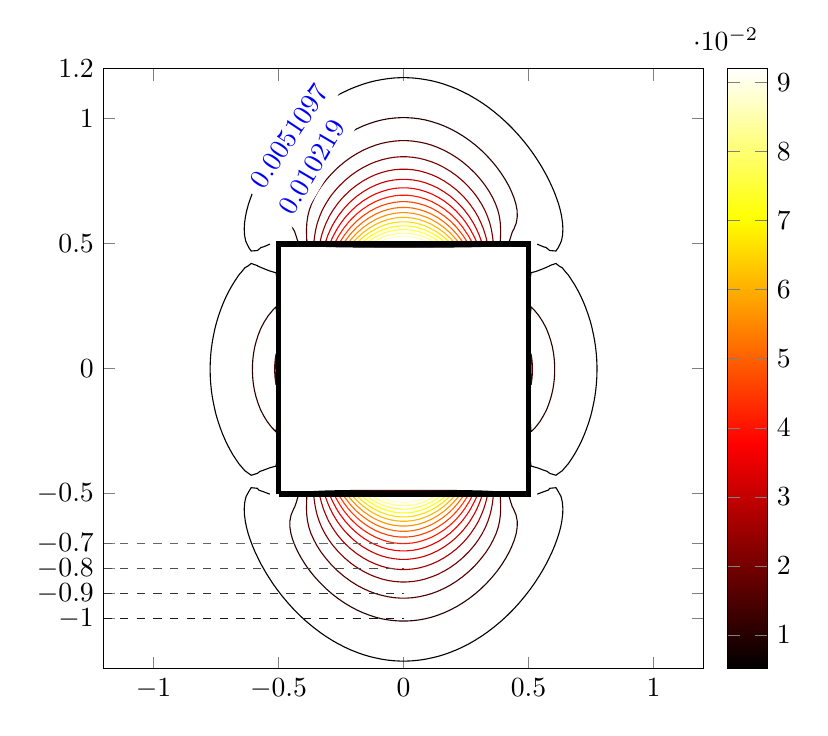
\begin{tikzpicture}

\begin{axis}[%
width=3in,
height=3in,
at={(0in,0in)},
scale only axis,
point meta min=0.0051,
point meta max=0.0920,
colormap/hot2,
xmin=-1.2000,
xmax=1.2000,
ymin=-1.2000,
ymax=1.2000,
ytick={-1.0000,-0.9000,-0.8000,-0.7000,-0.5000,0.0000,0.5000,1.0000,1.2000},
axis background/.style={fill=white},
colorbar
]
\addplot[contour prepared, contour prepared format=matlab, contour/labels=false] table[row sep=crcr] {%
%
0.0051	120.0000\\
-0.5348	0.4983\\
-0.5597	0.4878\\
-0.5701	0.4851\\
-0.5846	0.4729\\
-0.6095	0.4709\\
-0.6192	0.4851\\
-0.6311	0.5100\\
-0.6343	0.5250\\
-0.6360	0.5348\\
-0.6373	0.5597\\
-0.6359	0.5846\\
-0.6343	0.5945\\
-0.6323	0.6095\\
-0.6270	0.6343\\
-0.6201	0.6592\\
-0.6115	0.6841\\
-0.6095	0.6891\\
-0.6020	0.7090\\
-0.5912	0.7338\\
-0.5846	0.7474\\
-0.5793	0.7587\\
-0.5663	0.7836\\
-0.5597	0.7949\\
-0.5521	0.8085\\
-0.5366	0.8333\\
-0.5348	0.8359\\
-0.5201	0.8582\\
-0.5100	0.8723\\
-0.5022	0.8831\\
-0.4851	0.9048\\
-0.4826	0.9080\\
-0.4616	0.9328\\
-0.4602	0.9344\\
-0.4388	0.9577\\
-0.4353	0.9614\\
-0.4140	0.9826\\
-0.4104	0.9860\\
-0.3867	1.0075\\
-0.3856	1.0085\\
-0.3607	1.0292\\
-0.3567	1.0323\\
-0.3358	1.0483\\
-0.3229	1.0572\\
-0.3109	1.0655\\
-0.2861	1.0810\\
-0.2842	1.0821\\
-0.2612	1.0955\\
-0.2384	1.1070\\
-0.2363	1.1080\\
-0.2114	1.1197\\
-0.1866	1.1295\\
-0.1798	1.1318\\
-0.1617	1.1384\\
-0.1368	1.1459\\
-0.1119	1.1520\\
-0.0871	1.1567\\
-0.0869	1.1567\\
-0.0622	1.1605\\
-0.0373	1.1631\\
-0.0124	1.1643\\
0.0124	1.1643\\
0.0373	1.1631\\
0.0622	1.1605\\
0.0869	1.1567\\
0.0871	1.1567\\
0.1119	1.1520\\
0.1368	1.1459\\
0.1617	1.1384\\
0.1798	1.1318\\
0.1866	1.1295\\
0.2114	1.1197\\
0.2363	1.1080\\
0.2384	1.1070\\
0.2612	1.0955\\
0.2842	1.0821\\
0.2861	1.0810\\
0.3109	1.0655\\
0.3229	1.0572\\
0.3358	1.0483\\
0.3567	1.0323\\
0.3607	1.0292\\
0.3856	1.0085\\
0.3867	1.0075\\
0.4104	0.9860\\
0.4140	0.9826\\
0.4353	0.9614\\
0.4388	0.9577\\
0.4602	0.9344\\
0.4616	0.9328\\
0.4826	0.9080\\
0.4851	0.9048\\
0.5022	0.8831\\
0.5100	0.8723\\
0.5201	0.8582\\
0.5348	0.8359\\
0.5366	0.8333\\
0.5521	0.8085\\
0.5597	0.7949\\
0.5663	0.7836\\
0.5793	0.7587\\
0.5846	0.7474\\
0.5912	0.7338\\
0.6020	0.7090\\
0.6095	0.6891\\
0.6115	0.6841\\
0.6201	0.6592\\
0.6270	0.6343\\
0.6323	0.6095\\
0.6343	0.5945\\
0.6359	0.5846\\
0.6373	0.5597\\
0.6360	0.5348\\
0.6343	0.5250\\
0.6311	0.5100\\
0.6192	0.4851\\
0.6095	0.4709\\
0.5846	0.4729\\
0.5701	0.4851\\
0.5597	0.4878\\
0.5348	0.4983\\
0.0051	38.0000\\
-0.4602	-0.5070\\
-0.4353	-0.5000\\
-0.4104	-0.4960\\
-0.3856	-0.4933\\
-0.3607	-0.4914\\
-0.3358	-0.4901\\
-0.3109	-0.4891\\
-0.2861	-0.4885\\
-0.2612	-0.4879\\
-0.2363	-0.4875\\
-0.2114	-0.4872\\
-0.1866	-0.4870\\
-0.1617	-0.4868\\
-0.1368	-0.4867\\
-0.1119	-0.4866\\
-0.0871	-0.4865\\
-0.0622	-0.4864\\
-0.0373	-0.4864\\
-0.0124	-0.4864\\
0.0124	-0.4864\\
0.0373	-0.4864\\
0.0622	-0.4864\\
0.0871	-0.4865\\
0.1119	-0.4866\\
0.1368	-0.4867\\
0.1617	-0.4868\\
0.1866	-0.4870\\
0.2114	-0.4872\\
0.2363	-0.4875\\
0.2612	-0.4879\\
0.2861	-0.4885\\
0.3109	-0.4891\\
0.3358	-0.4901\\
0.3607	-0.4914\\
0.3856	-0.4933\\
0.4104	-0.4960\\
0.4353	-0.5000\\
0.4602	-0.5070\\
0.0051	38.0000\\
0.4602	0.5065\\
0.4353	0.4997\\
0.4104	0.4958\\
0.3856	0.4932\\
0.3607	0.4914\\
0.3358	0.4901\\
0.3109	0.4892\\
0.2861	0.4885\\
0.2612	0.4880\\
0.2363	0.4876\\
0.2114	0.4873\\
0.1866	0.4870\\
0.1617	0.4869\\
0.1368	0.4867\\
0.1119	0.4866\\
0.0871	0.4865\\
0.0622	0.4865\\
0.0373	0.4864\\
0.0124	0.4864\\
-0.0124	0.4864\\
-0.0373	0.4864\\
-0.0622	0.4865\\
-0.0871	0.4865\\
-0.1119	0.4866\\
-0.1368	0.4867\\
-0.1617	0.4869\\
-0.1866	0.4870\\
-0.2114	0.4873\\
-0.2363	0.4876\\
-0.2612	0.4880\\
-0.2861	0.4885\\
-0.3109	0.4892\\
-0.3358	0.4901\\
-0.3607	0.4914\\
-0.3856	0.4932\\
-0.4104	0.4958\\
-0.4353	0.4997\\
-0.4602	0.5065\\
0.0051	120.0000\\
0.5348	-0.5016\\
0.5597	-0.4922\\
0.5796	-0.4851\\
0.5846	-0.4783\\
0.6095	-0.4758\\
0.6155	-0.4851\\
0.6295	-0.5100\\
0.6343	-0.5294\\
0.6353	-0.5348\\
0.6373	-0.5597\\
0.6364	-0.5846\\
0.6343	-0.5995\\
0.6331	-0.6095\\
0.6282	-0.6343\\
0.6216	-0.6592\\
0.6133	-0.6841\\
0.6095	-0.6940\\
0.6040	-0.7090\\
0.5935	-0.7338\\
0.5846	-0.7524\\
0.5817	-0.7587\\
0.5690	-0.7836\\
0.5597	-0.7999\\
0.5550	-0.8085\\
0.5398	-0.8333\\
0.5348	-0.8409\\
0.5236	-0.8582\\
0.5100	-0.8772\\
0.5058	-0.8831\\
0.4866	-0.9080\\
0.4851	-0.9098\\
0.4660	-0.9328\\
0.4602	-0.9394\\
0.4436	-0.9577\\
0.4353	-0.9664\\
0.4192	-0.9826\\
0.4104	-0.9911\\
0.3925	-1.0075\\
0.3856	-1.0136\\
0.3629	-1.0323\\
0.3607	-1.0342\\
0.3358	-1.0531\\
0.3300	-1.0572\\
0.3109	-1.0705\\
0.2924	-1.0821\\
0.2861	-1.0861\\
0.2612	-1.1004\\
0.2482	-1.1070\\
0.2363	-1.1132\\
0.2114	-1.1246\\
0.1930	-1.1318\\
0.1866	-1.1345\\
0.1617	-1.1434\\
0.1368	-1.1508\\
0.1120	-1.1567\\
0.1119	-1.1567\\
0.0871	-1.1619\\
0.0622	-1.1656\\
0.0373	-1.1681\\
0.0124	-1.1694\\
-0.0124	-1.1694\\
-0.0373	-1.1681\\
-0.0622	-1.1656\\
-0.0871	-1.1619\\
-0.1119	-1.1567\\
-0.1120	-1.1567\\
-0.1368	-1.1508\\
-0.1617	-1.1434\\
-0.1866	-1.1345\\
-0.1930	-1.1318\\
-0.2114	-1.1246\\
-0.2363	-1.1132\\
-0.2482	-1.1070\\
-0.2612	-1.1004\\
-0.2861	-1.0861\\
-0.2924	-1.0821\\
-0.3109	-1.0705\\
-0.3300	-1.0572\\
-0.3358	-1.0531\\
-0.3607	-1.0342\\
-0.3629	-1.0323\\
-0.3856	-1.0136\\
-0.3925	-1.0075\\
-0.4104	-0.9911\\
-0.4192	-0.9826\\
-0.4353	-0.9664\\
-0.4436	-0.9577\\
-0.4602	-0.9394\\
-0.4660	-0.9328\\
-0.4851	-0.9098\\
-0.4866	-0.9080\\
-0.5058	-0.8831\\
-0.5100	-0.8772\\
-0.5236	-0.8582\\
-0.5348	-0.8409\\
-0.5398	-0.8333\\
-0.5550	-0.8085\\
-0.5597	-0.7999\\
-0.5690	-0.7836\\
-0.5817	-0.7587\\
-0.5846	-0.7524\\
-0.5935	-0.7338\\
-0.6040	-0.7090\\
-0.6095	-0.6940\\
-0.6133	-0.6841\\
-0.6216	-0.6592\\
-0.6282	-0.6343\\
-0.6331	-0.6095\\
-0.6343	-0.5995\\
-0.6364	-0.5846\\
-0.6373	-0.5597\\
-0.6353	-0.5348\\
-0.6343	-0.5294\\
-0.6295	-0.5100\\
-0.6155	-0.4851\\
-0.6095	-0.4758\\
-0.5846	-0.4783\\
-0.5796	-0.4851\\
-0.5597	-0.4922\\
-0.5348	-0.5016\\
0.0051	91.0000\\
-0.7587	-0.1454\\
-0.7606	-0.1368\\
-0.7651	-0.1119\\
-0.7686	-0.0871\\
-0.7712	-0.0622\\
-0.7729	-0.0373\\
-0.7736	-0.0124\\
-0.7736	0.0124\\
-0.7726	0.0373\\
-0.7708	0.0622\\
-0.7680	0.0871\\
-0.7643	0.1119\\
-0.7596	0.1368\\
-0.7587	0.1406\\
-0.7542	0.1617\\
-0.7478	0.1866\\
-0.7402	0.2114\\
-0.7338	0.2297\\
-0.7315	0.2363\\
-0.7219	0.2612\\
-0.7108	0.2861\\
-0.7090	0.2899\\
-0.6984	0.3109\\
-0.6845	0.3358\\
-0.6841	0.3365\\
-0.6684	0.3607\\
-0.6592	0.3747\\
-0.6495	0.3856\\
-0.6343	0.4043\\
-0.6230	0.4104\\
-0.6095	0.4212\\
-0.5846	0.4125\\
-0.5827	0.4104\\
-0.5597	0.4007\\
-0.5348	0.3910\\
-0.5161	0.3856\\
-0.5100	0.3843\\
-0.5065	0.3607\\
-0.5036	0.3358\\
-0.5014	0.3109\\
-0.4996	0.2861\\
-0.4982	0.2612\\
-0.4970	0.2363\\
-0.4961	0.2114\\
-0.4954	0.1866\\
-0.4948	0.1617\\
-0.4943	0.1368\\
-0.4939	0.1119\\
-0.4936	0.0871\\
-0.4934	0.0622\\
-0.4932	0.0373\\
-0.4932	0.0124\\
-0.4932	-0.0124\\
-0.4932	-0.0373\\
-0.4933	-0.0622\\
-0.4935	-0.0871\\
-0.4938	-0.1119\\
-0.4942	-0.1368\\
-0.4946	-0.1617\\
-0.4952	-0.1866\\
-0.4959	-0.2114\\
-0.4968	-0.2363\\
-0.4979	-0.2612\\
-0.4993	-0.2861\\
-0.5010	-0.3109\\
-0.5032	-0.3358\\
-0.5059	-0.3607\\
-0.5094	-0.3856\\
-0.5100	-0.3894\\
-0.5348	-0.3961\\
-0.5597	-0.4055\\
-0.5743	-0.4104\\
-0.5846	-0.4185\\
-0.6095	-0.4260\\
-0.6310	-0.4104\\
-0.6343	-0.4086\\
-0.6538	-0.3856\\
-0.6592	-0.3795\\
-0.6718	-0.3607\\
-0.6841	-0.3417\\
-0.6874	-0.3358\\
-0.7010	-0.3109\\
-0.7090	-0.2949\\
-0.7131	-0.2861\\
-0.7239	-0.2612\\
-0.7333	-0.2363\\
-0.7338	-0.2347\\
-0.7418	-0.2114\\
-0.7492	-0.1866\\
-0.7553	-0.1617\\
-0.7587	-0.1454\\
0.0051	91.0000\\
0.5100	-0.3894\\
0.5094	-0.3856\\
0.5059	-0.3607\\
0.5032	-0.3358\\
0.5010	-0.3109\\
0.4993	-0.2861\\
0.4979	-0.2612\\
0.4968	-0.2363\\
0.4959	-0.2114\\
0.4952	-0.1866\\
0.4946	-0.1617\\
0.4942	-0.1368\\
0.4938	-0.1119\\
0.4935	-0.0871\\
0.4933	-0.0622\\
0.4932	-0.0373\\
0.4932	-0.0124\\
0.4932	0.0124\\
0.4932	0.0373\\
0.4934	0.0622\\
0.4936	0.0871\\
0.4939	0.1119\\
0.4943	0.1368\\
0.4948	0.1617\\
0.4954	0.1866\\
0.4961	0.2114\\
0.4970	0.2363\\
0.4982	0.2612\\
0.4996	0.2861\\
0.5014	0.3109\\
0.5036	0.3358\\
0.5065	0.3607\\
0.5100	0.3843\\
0.5161	0.3856\\
0.5348	0.3910\\
0.5597	0.4007\\
0.5827	0.4104\\
0.5846	0.4125\\
0.6095	0.4212\\
0.6230	0.4104\\
0.6343	0.4043\\
0.6495	0.3856\\
0.6592	0.3747\\
0.6684	0.3607\\
0.6841	0.3365\\
0.6845	0.3358\\
0.6984	0.3109\\
0.7090	0.2899\\
0.7108	0.2861\\
0.7219	0.2612\\
0.7315	0.2363\\
0.7338	0.2297\\
0.7402	0.2114\\
0.7478	0.1866\\
0.7542	0.1617\\
0.7587	0.1406\\
0.7596	0.1368\\
0.7643	0.1119\\
0.7680	0.0871\\
0.7708	0.0622\\
0.7726	0.0373\\
0.7736	0.0124\\
0.7736	-0.0124\\
0.7729	-0.0373\\
0.7712	-0.0622\\
0.7686	-0.0871\\
0.7651	-0.1119\\
0.7606	-0.1368\\
0.7587	-0.1454\\
0.7553	-0.1617\\
0.7492	-0.1866\\
0.7418	-0.2114\\
0.7338	-0.2347\\
0.7333	-0.2363\\
0.7239	-0.2612\\
0.7131	-0.2861\\
0.7090	-0.2949\\
0.7010	-0.3109\\
0.6874	-0.3358\\
0.6841	-0.3417\\
0.6718	-0.3607\\
0.6592	-0.3795\\
0.6538	-0.3856\\
0.6343	-0.4086\\
0.6310	-0.4104\\
0.6095	-0.4260\\
0.5846	-0.4185\\
0.5743	-0.4104\\
0.5597	-0.4055\\
0.5348	-0.3961\\
0.5100	-0.3894\\
0.0102	49.0000\\
-0.5846	-0.1299\\
-0.5903	-0.1119\\
-0.5964	-0.0871\\
-0.6006	-0.0622\\
-0.6033	-0.0373\\
-0.6045	-0.0124\\
-0.6044	0.0124\\
-0.6029	0.0373\\
-0.5999	0.0622\\
-0.5953	0.0871\\
-0.5889	0.1119\\
-0.5846	0.1248\\
-0.5808	0.1368\\
-0.5708	0.1617\\
-0.5597	0.1827\\
-0.5577	0.1866\\
-0.5418	0.2114\\
-0.5348	0.2201\\
-0.5213	0.2363\\
-0.5100	0.2472\\
-0.5090	0.2363\\
-0.5071	0.2114\\
-0.5056	0.1866\\
-0.5044	0.1617\\
-0.5035	0.1368\\
-0.5027	0.1119\\
-0.5021	0.0871\\
-0.5017	0.0622\\
-0.5014	0.0373\\
-0.5013	0.0124\\
-0.5012	-0.0124\\
-0.5014	-0.0373\\
-0.5016	-0.0622\\
-0.5020	-0.0871\\
-0.5026	-0.1119\\
-0.5033	-0.1368\\
-0.5042	-0.1617\\
-0.5054	-0.1866\\
-0.5068	-0.2114\\
-0.5086	-0.2363\\
-0.5100	-0.2522\\
-0.5259	-0.2363\\
-0.5348	-0.2251\\
-0.5454	-0.2114\\
-0.5597	-0.1877\\
-0.5604	-0.1866\\
-0.5730	-0.1617\\
-0.5825	-0.1368\\
-0.5846	-0.1299\\
0.0102	115.0000\\
-0.4353	-0.7044\\
-0.4434	-0.6841\\
-0.4505	-0.6592\\
-0.4545	-0.6343\\
-0.4547	-0.6095\\
-0.4499	-0.5846\\
-0.4393	-0.5597\\
-0.4353	-0.5527\\
-0.4291	-0.5348\\
-0.4219	-0.5100\\
-0.4104	-0.5068\\
-0.3856	-0.5014\\
-0.3607	-0.4977\\
-0.3358	-0.4951\\
-0.3109	-0.4932\\
-0.2861	-0.4918\\
-0.2612	-0.4908\\
-0.2363	-0.4900\\
-0.2114	-0.4894\\
-0.1866	-0.4889\\
-0.1617	-0.4886\\
-0.1368	-0.4883\\
-0.1119	-0.4881\\
-0.0871	-0.4879\\
-0.0622	-0.4878\\
-0.0373	-0.4877\\
-0.0124	-0.4877\\
0.0124	-0.4877\\
0.0373	-0.4877\\
0.0622	-0.4878\\
0.0871	-0.4879\\
0.1119	-0.4881\\
0.1368	-0.4883\\
0.1617	-0.4886\\
0.1866	-0.4889\\
0.2114	-0.4894\\
0.2363	-0.4900\\
0.2612	-0.4908\\
0.2861	-0.4918\\
0.3109	-0.4932\\
0.3358	-0.4951\\
0.3607	-0.4977\\
0.3856	-0.5014\\
0.4104	-0.5068\\
0.4219	-0.5100\\
0.4291	-0.5348\\
0.4353	-0.5527\\
0.4393	-0.5597\\
0.4499	-0.5846\\
0.4547	-0.6095\\
0.4545	-0.6343\\
0.4505	-0.6592\\
0.4434	-0.6841\\
0.4353	-0.7044\\
0.4336	-0.7090\\
0.4223	-0.7338\\
0.4104	-0.7549\\
0.4083	-0.7587\\
0.3928	-0.7836\\
0.3856	-0.7937\\
0.3749	-0.8085\\
0.3607	-0.8262\\
0.3547	-0.8333\\
0.3358	-0.8541\\
0.3319	-0.8582\\
0.3109	-0.8788\\
0.3062	-0.8831\\
0.2861	-0.9006\\
0.2767	-0.9080\\
0.2612	-0.9199\\
0.2422	-0.9328\\
0.2363	-0.9368\\
0.2114	-0.9519\\
0.2003	-0.9577\\
0.1866	-0.9650\\
0.1617	-0.9763\\
0.1450	-0.9826\\
0.1368	-0.9858\\
0.1119	-0.9939\\
0.0871	-1.0001\\
0.0622	-1.0046\\
0.0383	-1.0075\\
0.0373	-1.0076\\
0.0124	-1.0092\\
-0.0124	-1.0092\\
-0.0373	-1.0076\\
-0.0383	-1.0075\\
-0.0622	-1.0046\\
-0.0871	-1.0001\\
-0.1119	-0.9939\\
-0.1368	-0.9858\\
-0.1450	-0.9826\\
-0.1617	-0.9763\\
-0.1866	-0.9650\\
-0.2003	-0.9577\\
-0.2114	-0.9519\\
-0.2363	-0.9368\\
-0.2422	-0.9328\\
-0.2612	-0.9199\\
-0.2767	-0.9080\\
-0.2861	-0.9006\\
-0.3062	-0.8831\\
-0.3109	-0.8788\\
-0.3319	-0.8582\\
-0.3358	-0.8541\\
-0.3547	-0.8333\\
-0.3607	-0.8262\\
-0.3749	-0.8085\\
-0.3856	-0.7937\\
-0.3928	-0.7836\\
-0.4083	-0.7587\\
-0.4104	-0.7549\\
-0.4223	-0.7338\\
-0.4336	-0.7090\\
-0.4353	-0.7044\\
0.0102	113.0000\\
-0.4353	0.5481\\
-0.4418	0.5597\\
-0.4513	0.5846\\
-0.4550	0.6095\\
-0.4540	0.6343\\
-0.4493	0.6592\\
-0.4416	0.6841\\
-0.4353	0.6993\\
-0.4316	0.7090\\
-0.4197	0.7338\\
-0.4104	0.7499\\
-0.4055	0.7587\\
-0.3893	0.7836\\
-0.3856	0.7887\\
-0.3711	0.8085\\
-0.3607	0.8212\\
-0.3504	0.8333\\
-0.3358	0.8492\\
-0.3271	0.8582\\
-0.3109	0.8739\\
-0.3006	0.8831\\
-0.2861	0.8957\\
-0.2702	0.9080\\
-0.2612	0.9149\\
-0.2363	0.9318\\
-0.2345	0.9328\\
-0.2114	0.9470\\
-0.1907	0.9577\\
-0.1866	0.9599\\
-0.1617	0.9714\\
-0.1368	0.9808\\
-0.1309	0.9826\\
-0.1119	0.9888\\
-0.0871	0.9952\\
-0.0622	0.9998\\
-0.0373	1.0028\\
-0.0124	1.0043\\
0.0124	1.0043\\
0.0373	1.0028\\
0.0622	0.9998\\
0.0871	0.9952\\
0.1119	0.9888\\
0.1309	0.9826\\
0.1368	0.9808\\
0.1617	0.9714\\
0.1866	0.9599\\
0.1907	0.9577\\
0.2114	0.9470\\
0.2345	0.9328\\
0.2363	0.9318\\
0.2612	0.9149\\
0.2702	0.9080\\
0.2861	0.8957\\
0.3006	0.8831\\
0.3109	0.8739\\
0.3271	0.8582\\
0.3358	0.8492\\
0.3504	0.8333\\
0.3607	0.8212\\
0.3711	0.8085\\
0.3856	0.7887\\
0.3893	0.7836\\
0.4055	0.7587\\
0.4104	0.7499\\
0.4197	0.7338\\
0.4316	0.7090\\
0.4353	0.6993\\
0.4416	0.6841\\
0.4493	0.6592\\
0.4540	0.6343\\
0.4550	0.6095\\
0.4513	0.5846\\
0.4418	0.5597\\
0.4353	0.5481\\
0.4309	0.5348\\
0.4232	0.5100\\
0.4104	0.5066\\
0.3856	0.5014\\
0.3607	0.4978\\
0.3358	0.4952\\
0.3109	0.4933\\
0.2861	0.4919\\
0.2612	0.4909\\
0.2363	0.4901\\
0.2114	0.4895\\
0.1866	0.4890\\
0.1617	0.4886\\
0.1368	0.4884\\
0.1119	0.4881\\
0.0871	0.4880\\
0.0622	0.4879\\
0.0373	0.4878\\
0.0124	0.4878\\
-0.0124	0.4878\\
-0.0373	0.4878\\
-0.0622	0.4879\\
-0.0871	0.4880\\
-0.1119	0.4881\\
-0.1368	0.4884\\
-0.1617	0.4886\\
-0.1866	0.4890\\
-0.2114	0.4895\\
-0.2363	0.4901\\
-0.2612	0.4909\\
-0.2861	0.4919\\
-0.3109	0.4933\\
-0.3358	0.4952\\
-0.3607	0.4978\\
-0.3856	0.5014\\
-0.4104	0.5066\\
-0.4232	0.5100\\
-0.4309	0.5348\\
-0.4353	0.5481\\
0.0102	49.0000\\
0.5100	-0.2522\\
0.5086	-0.2363\\
0.5068	-0.2114\\
0.5054	-0.1866\\
0.5042	-0.1617\\
0.5033	-0.1368\\
0.5026	-0.1119\\
0.5020	-0.0871\\
0.5016	-0.0622\\
0.5014	-0.0373\\
0.5012	-0.0124\\
0.5013	0.0124\\
0.5014	0.0373\\
0.5017	0.0622\\
0.5021	0.0871\\
0.5027	0.1119\\
0.5035	0.1368\\
0.5044	0.1617\\
0.5056	0.1866\\
0.5071	0.2114\\
0.5090	0.2363\\
0.5100	0.2472\\
0.5213	0.2363\\
0.5348	0.2201\\
0.5418	0.2114\\
0.5577	0.1866\\
0.5597	0.1827\\
0.5708	0.1617\\
0.5808	0.1368\\
0.5846	0.1248\\
0.5889	0.1119\\
0.5953	0.0871\\
0.5999	0.0622\\
0.6029	0.0373\\
0.6044	0.0124\\
0.6045	-0.0124\\
0.6033	-0.0373\\
0.6006	-0.0622\\
0.5964	-0.0871\\
0.5903	-0.1119\\
0.5846	-0.1299\\
0.5825	-0.1368\\
0.5730	-0.1617\\
0.5604	-0.1866\\
0.5597	-0.1877\\
0.5454	-0.2114\\
0.5348	-0.2251\\
0.5259	-0.2363\\
0.5100	-0.2522\\
0.0153	13.0000\\
-0.5100	-0.0649\\
-0.5105	-0.0622\\
-0.5139	-0.0373\\
-0.5155	-0.0124\\
-0.5154	0.0124\\
-0.5134	0.0373\\
-0.5100	0.0600\\
-0.5096	0.0373\\
-0.5094	0.0124\\
-0.5093	-0.0124\\
-0.5095	-0.0373\\
-0.5099	-0.0622\\
-0.5100	-0.0649\\
0.0153	99.0000\\
-0.3856	-0.5974\\
-0.3873	-0.5846\\
-0.3883	-0.5597\\
-0.3879	-0.5348\\
-0.3869	-0.5100\\
-0.3856	-0.5096\\
-0.3607	-0.5041\\
-0.3358	-0.5001\\
-0.3109	-0.4973\\
-0.2861	-0.4952\\
-0.2612	-0.4936\\
-0.2363	-0.4925\\
-0.2114	-0.4916\\
-0.1866	-0.4909\\
-0.1617	-0.4903\\
-0.1368	-0.4899\\
-0.1119	-0.4896\\
-0.0871	-0.4893\\
-0.0622	-0.4892\\
-0.0373	-0.4891\\
-0.0124	-0.4890\\
0.0124	-0.4890\\
0.0373	-0.4891\\
0.0622	-0.4892\\
0.0871	-0.4893\\
0.1119	-0.4896\\
0.1368	-0.4899\\
0.1617	-0.4903\\
0.1866	-0.4909\\
0.2114	-0.4916\\
0.2363	-0.4925\\
0.2612	-0.4936\\
0.2861	-0.4952\\
0.3109	-0.4973\\
0.3358	-0.5001\\
0.3607	-0.5041\\
0.3856	-0.5096\\
0.3869	-0.5100\\
0.3879	-0.5348\\
0.3883	-0.5597\\
0.3873	-0.5846\\
0.3856	-0.5974\\
0.3841	-0.6095\\
0.3785	-0.6343\\
0.3702	-0.6592\\
0.3607	-0.6801\\
0.3589	-0.6841\\
0.3457	-0.7090\\
0.3358	-0.7244\\
0.3296	-0.7338\\
0.3109	-0.7584\\
0.3107	-0.7587\\
0.2891	-0.7836\\
0.2861	-0.7869\\
0.2640	-0.8085\\
0.2612	-0.8110\\
0.2363	-0.8319\\
0.2344	-0.8333\\
0.2114	-0.8501\\
0.1985	-0.8582\\
0.1866	-0.8657\\
0.1617	-0.8789\\
0.1523	-0.8831\\
0.1368	-0.8902\\
0.1119	-0.8994\\
0.0871	-0.9065\\
0.0799	-0.9080\\
0.0622	-0.9120\\
0.0373	-0.9157\\
0.0124	-0.9175\\
-0.0124	-0.9175\\
-0.0373	-0.9157\\
-0.0622	-0.9120\\
-0.0799	-0.9080\\
-0.0871	-0.9065\\
-0.1119	-0.8994\\
-0.1368	-0.8902\\
-0.1523	-0.8831\\
-0.1617	-0.8789\\
-0.1866	-0.8657\\
-0.1985	-0.8582\\
-0.2114	-0.8501\\
-0.2344	-0.8333\\
-0.2363	-0.8319\\
-0.2612	-0.8110\\
-0.2640	-0.8085\\
-0.2861	-0.7869\\
-0.2891	-0.7836\\
-0.3107	-0.7587\\
-0.3109	-0.7584\\
-0.3296	-0.7338\\
-0.3358	-0.7244\\
-0.3457	-0.7090\\
-0.3589	-0.6841\\
-0.3607	-0.6801\\
-0.3702	-0.6592\\
-0.3785	-0.6343\\
-0.3841	-0.6095\\
-0.3856	-0.5974\\
0.0153	99.0000\\
-0.3856	0.5096\\
-0.3871	0.5100\\
-0.3880	0.5348\\
-0.3882	0.5597\\
-0.3868	0.5846\\
-0.3856	0.5927\\
-0.3832	0.6095\\
-0.3771	0.6343\\
-0.3681	0.6592\\
-0.3607	0.6751\\
-0.3565	0.6841\\
-0.3426	0.7090\\
-0.3358	0.7194\\
-0.3261	0.7338\\
-0.3109	0.7536\\
-0.3067	0.7587\\
-0.2861	0.7819\\
-0.2844	0.7836\\
-0.2612	0.8061\\
-0.2584	0.8085\\
-0.2363	0.8271\\
-0.2278	0.8333\\
-0.2114	0.8452\\
-0.1904	0.8582\\
-0.1866	0.8606\\
-0.1617	0.8741\\
-0.1411	0.8831\\
-0.1368	0.8851\\
-0.1119	0.8945\\
-0.0871	0.9017\\
-0.0622	0.9069\\
-0.0543	0.9080\\
-0.0373	0.9105\\
-0.0124	0.9124\\
0.0124	0.9124\\
0.0373	0.9105\\
0.0543	0.9080\\
0.0622	0.9069\\
0.0871	0.9017\\
0.1119	0.8945\\
0.1368	0.8851\\
0.1411	0.8831\\
0.1617	0.8741\\
0.1866	0.8606\\
0.1904	0.8582\\
0.2114	0.8452\\
0.2278	0.8333\\
0.2363	0.8271\\
0.2584	0.8085\\
0.2612	0.8061\\
0.2844	0.7836\\
0.2861	0.7819\\
0.3067	0.7587\\
0.3109	0.7536\\
0.3261	0.7338\\
0.3358	0.7194\\
0.3426	0.7090\\
0.3565	0.6841\\
0.3607	0.6751\\
0.3681	0.6592\\
0.3771	0.6343\\
0.3832	0.6095\\
0.3856	0.5927\\
0.3868	0.5846\\
0.3882	0.5597\\
0.3880	0.5348\\
0.3871	0.5100\\
0.3856	0.5096\\
0.3607	0.5042\\
0.3358	0.5003\\
0.3109	0.4975\\
0.2861	0.4954\\
0.2612	0.4938\\
0.2363	0.4926\\
0.2114	0.4917\\
0.1866	0.4910\\
0.1617	0.4904\\
0.1368	0.4900\\
0.1119	0.4897\\
0.0871	0.4894\\
0.0622	0.4893\\
0.0373	0.4891\\
0.0124	0.4891\\
-0.0124	0.4891\\
-0.0373	0.4891\\
-0.0622	0.4893\\
-0.0871	0.4894\\
-0.1119	0.4897\\
-0.1368	0.4900\\
-0.1617	0.4904\\
-0.1866	0.4910\\
-0.2114	0.4917\\
-0.2363	0.4926\\
-0.2612	0.4938\\
-0.2861	0.4954\\
-0.3109	0.4975\\
-0.3358	0.5003\\
-0.3607	0.5042\\
-0.3856	0.5096\\
0.0153	13.0000\\
0.5100	-0.0649\\
0.5099	-0.0622\\
0.5095	-0.0373\\
0.5093	-0.0124\\
0.5094	0.0124\\
0.5096	0.0373\\
0.5100	0.0600\\
0.5134	0.0373\\
0.5154	0.0124\\
0.5155	-0.0124\\
0.5139	-0.0373\\
0.5105	-0.0622\\
0.5100	-0.0649\\
0.0204	85.0000\\
-0.3358	-0.6138\\
-0.3376	-0.6095\\
-0.3458	-0.5846\\
-0.3517	-0.5597\\
-0.3559	-0.5348\\
-0.3590	-0.5100\\
-0.3358	-0.5052\\
-0.3109	-0.5014\\
-0.2861	-0.4986\\
-0.2612	-0.4965\\
-0.2363	-0.4949\\
-0.2114	-0.4937\\
-0.1866	-0.4928\\
-0.1617	-0.4921\\
-0.1368	-0.4915\\
-0.1119	-0.4911\\
-0.0871	-0.4908\\
-0.0622	-0.4905\\
-0.0373	-0.4904\\
-0.0124	-0.4903\\
0.0124	-0.4903\\
0.0373	-0.4904\\
0.0622	-0.4905\\
0.0871	-0.4908\\
0.1119	-0.4911\\
0.1368	-0.4915\\
0.1617	-0.4921\\
0.1866	-0.4928\\
0.2114	-0.4937\\
0.2363	-0.4949\\
0.2612	-0.4965\\
0.2861	-0.4986\\
0.3109	-0.5014\\
0.3358	-0.5052\\
0.3590	-0.5100\\
0.3559	-0.5348\\
0.3517	-0.5597\\
0.3458	-0.5846\\
0.3376	-0.6095\\
0.3358	-0.6138\\
0.3275	-0.6343\\
0.3145	-0.6592\\
0.3109	-0.6653\\
0.2992	-0.6841\\
0.2861	-0.7022\\
0.2808	-0.7090\\
0.2612	-0.7317\\
0.2591	-0.7338\\
0.2363	-0.7563\\
0.2335	-0.7587\\
0.2114	-0.7773\\
0.2027	-0.7836\\
0.1866	-0.7951\\
0.1640	-0.8085\\
0.1617	-0.8099\\
0.1368	-0.8226\\
0.1119	-0.8326\\
0.1096	-0.8333\\
0.0871	-0.8409\\
0.0622	-0.8470\\
0.0373	-0.8509\\
0.0124	-0.8528\\
-0.0124	-0.8528\\
-0.0373	-0.8509\\
-0.0622	-0.8470\\
-0.0871	-0.8409\\
-0.1096	-0.8333\\
-0.1119	-0.8326\\
-0.1368	-0.8226\\
-0.1617	-0.8099\\
-0.1640	-0.8085\\
-0.1866	-0.7951\\
-0.2027	-0.7836\\
-0.2114	-0.7773\\
-0.2335	-0.7587\\
-0.2363	-0.7563\\
-0.2591	-0.7338\\
-0.2612	-0.7317\\
-0.2808	-0.7090\\
-0.2861	-0.7022\\
-0.2992	-0.6841\\
-0.3109	-0.6653\\
-0.3145	-0.6592\\
-0.3275	-0.6343\\
-0.3358	-0.6138\\
0.0204	85.0000\\
-0.3358	0.5054\\
-0.3584	0.5100\\
-0.3552	0.5348\\
-0.3507	0.5597\\
-0.3444	0.5846\\
-0.3358	0.6089\\
-0.3356	0.6095\\
-0.3251	0.6343\\
-0.3116	0.6592\\
-0.3109	0.6602\\
-0.2958	0.6841\\
-0.2861	0.6973\\
-0.2768	0.7090\\
-0.2612	0.7268\\
-0.2544	0.7338\\
-0.2363	0.7515\\
-0.2279	0.7587\\
-0.2114	0.7724\\
-0.1957	0.7836\\
-0.1866	0.7901\\
-0.1617	0.8050\\
-0.1547	0.8085\\
-0.1368	0.8177\\
-0.1119	0.8278\\
-0.0944	0.8333\\
-0.0871	0.8358\\
-0.0622	0.8419\\
-0.0373	0.8459\\
-0.0124	0.8479\\
0.0124	0.8479\\
0.0373	0.8459\\
0.0622	0.8419\\
0.0871	0.8358\\
0.0944	0.8333\\
0.1119	0.8278\\
0.1368	0.8177\\
0.1547	0.8085\\
0.1617	0.8050\\
0.1866	0.7901\\
0.1957	0.7836\\
0.2114	0.7724\\
0.2279	0.7587\\
0.2363	0.7515\\
0.2544	0.7338\\
0.2612	0.7268\\
0.2768	0.7090\\
0.2861	0.6973\\
0.2958	0.6841\\
0.3109	0.6602\\
0.3116	0.6592\\
0.3251	0.6343\\
0.3356	0.6095\\
0.3358	0.6089\\
0.3444	0.5846\\
0.3507	0.5597\\
0.3552	0.5348\\
0.3584	0.5100\\
0.3358	0.5054\\
0.3109	0.5016\\
0.2861	0.4988\\
0.2612	0.4967\\
0.2363	0.4951\\
0.2114	0.4939\\
0.1866	0.4929\\
0.1617	0.4922\\
0.1368	0.4916\\
0.1119	0.4912\\
0.0871	0.4909\\
0.0622	0.4907\\
0.0373	0.4905\\
0.0124	0.4904\\
-0.0124	0.4904\\
-0.0373	0.4905\\
-0.0622	0.4907\\
-0.0871	0.4909\\
-0.1119	0.4912\\
-0.1368	0.4916\\
-0.1617	0.4922\\
-0.1866	0.4929\\
-0.2114	0.4939\\
-0.2363	0.4951\\
-0.2612	0.4967\\
-0.2861	0.4988\\
-0.3109	0.5016\\
-0.3358	0.5054\\
0.0255	77.0000\\
-0.3109	-0.5852\\
-0.3112	-0.5846\\
-0.3210	-0.5597\\
-0.3287	-0.5348\\
-0.3348	-0.5100\\
-0.3109	-0.5054\\
-0.2861	-0.5020\\
-0.2612	-0.4994\\
-0.2363	-0.4974\\
-0.2114	-0.4959\\
-0.1866	-0.4947\\
-0.1617	-0.4938\\
-0.1368	-0.4931\\
-0.1119	-0.4926\\
-0.0871	-0.4922\\
-0.0622	-0.4919\\
-0.0373	-0.4917\\
-0.0124	-0.4916\\
0.0124	-0.4916\\
0.0373	-0.4917\\
0.0622	-0.4919\\
0.0871	-0.4922\\
0.1119	-0.4926\\
0.1368	-0.4931\\
0.1617	-0.4938\\
0.1866	-0.4947\\
0.2114	-0.4959\\
0.2363	-0.4974\\
0.2612	-0.4994\\
0.2861	-0.5020\\
0.3109	-0.5054\\
0.3348	-0.5100\\
0.3287	-0.5348\\
0.3210	-0.5597\\
0.3112	-0.5846\\
0.3109	-0.5852\\
0.2997	-0.6095\\
0.2861	-0.6331\\
0.2853	-0.6343\\
0.2684	-0.6592\\
0.2612	-0.6687\\
0.2482	-0.6841\\
0.2363	-0.6971\\
0.2240	-0.7090\\
0.2114	-0.7206\\
0.1947	-0.7338\\
0.1866	-0.7401\\
0.1617	-0.7565\\
0.1576	-0.7587\\
0.1368	-0.7704\\
0.1119	-0.7813\\
0.1052	-0.7836\\
0.0871	-0.7902\\
0.0622	-0.7967\\
0.0373	-0.8009\\
0.0124	-0.8030\\
-0.0124	-0.8030\\
-0.0373	-0.8009\\
-0.0622	-0.7967\\
-0.0871	-0.7902\\
-0.1052	-0.7836\\
-0.1119	-0.7813\\
-0.1368	-0.7704\\
-0.1576	-0.7587\\
-0.1617	-0.7565\\
-0.1866	-0.7401\\
-0.1947	-0.7338\\
-0.2114	-0.7206\\
-0.2240	-0.7090\\
-0.2363	-0.6971\\
-0.2482	-0.6841\\
-0.2612	-0.6687\\
-0.2684	-0.6592\\
-0.2853	-0.6343\\
-0.2861	-0.6331\\
-0.2997	-0.6095\\
-0.3109	-0.5852\\
0.0255	77.0000\\
-0.3109	0.5057\\
-0.3337	0.5100\\
-0.3273	0.5348\\
-0.3193	0.5597\\
-0.3109	0.5803\\
-0.3091	0.5846\\
-0.2971	0.6095\\
-0.2861	0.6282\\
-0.2822	0.6343\\
-0.2646	0.6592\\
-0.2612	0.6636\\
-0.2437	0.6841\\
-0.2363	0.6921\\
-0.2186	0.7090\\
-0.2114	0.7155\\
-0.1881	0.7338\\
-0.1866	0.7350\\
-0.1617	0.7517\\
-0.1487	0.7587\\
-0.1368	0.7653\\
-0.1119	0.7765\\
-0.0910	0.7836\\
-0.0871	0.7850\\
-0.0622	0.7917\\
-0.0373	0.7960\\
-0.0124	0.7981\\
0.0124	0.7981\\
0.0373	0.7960\\
0.0622	0.7917\\
0.0871	0.7850\\
0.0910	0.7836\\
0.1119	0.7765\\
0.1368	0.7653\\
0.1487	0.7587\\
0.1617	0.7517\\
0.1866	0.7350\\
0.1881	0.7338\\
0.2114	0.7155\\
0.2186	0.7090\\
0.2363	0.6921\\
0.2437	0.6841\\
0.2612	0.6636\\
0.2646	0.6592\\
0.2822	0.6343\\
0.2861	0.6282\\
0.2971	0.6095\\
0.3091	0.5846\\
0.3109	0.5803\\
0.3193	0.5597\\
0.3273	0.5348\\
0.3337	0.5100\\
0.3109	0.5057\\
0.2861	0.5022\\
0.2612	0.4996\\
0.2363	0.4976\\
0.2114	0.4961\\
0.1866	0.4949\\
0.1617	0.4940\\
0.1368	0.4933\\
0.1119	0.4927\\
0.0871	0.4923\\
0.0622	0.4920\\
0.0373	0.4919\\
0.0124	0.4918\\
-0.0124	0.4918\\
-0.0373	0.4919\\
-0.0622	0.4920\\
-0.0871	0.4923\\
-0.1119	0.4927\\
-0.1368	0.4933\\
-0.1617	0.4940\\
-0.1866	0.4949\\
-0.2114	0.4961\\
-0.2363	0.4976\\
-0.2612	0.4996\\
-0.2861	0.5022\\
-0.3109	0.5057\\
0.0307	75.0000\\
-0.3109	-0.5166\\
-0.3132	-0.5100\\
-0.3109	-0.5095\\
-0.2861	-0.5053\\
-0.2612	-0.5022\\
-0.2363	-0.4999\\
-0.2114	-0.4980\\
-0.1866	-0.4966\\
-0.1617	-0.4955\\
-0.1368	-0.4947\\
-0.1119	-0.4941\\
-0.0871	-0.4936\\
-0.0622	-0.4933\\
-0.0373	-0.4930\\
-0.0124	-0.4929\\
0.0124	-0.4929\\
0.0373	-0.4930\\
0.0622	-0.4933\\
0.0871	-0.4936\\
0.1119	-0.4941\\
0.1368	-0.4947\\
0.1617	-0.4955\\
0.1866	-0.4966\\
0.2114	-0.4980\\
0.2363	-0.4999\\
0.2612	-0.5022\\
0.2861	-0.5053\\
0.3109	-0.5095\\
0.3132	-0.5100\\
0.3109	-0.5166\\
0.3043	-0.5348\\
0.2937	-0.5597\\
0.2861	-0.5751\\
0.2809	-0.5846\\
0.2658	-0.6095\\
0.2612	-0.6162\\
0.2477	-0.6343\\
0.2363	-0.6482\\
0.2260	-0.6592\\
0.2114	-0.6740\\
0.1999	-0.6841\\
0.1866	-0.6954\\
0.1674	-0.7090\\
0.1617	-0.7130\\
0.1368	-0.7277\\
0.1238	-0.7338\\
0.1119	-0.7396\\
0.0871	-0.7490\\
0.0622	-0.7557\\
0.0447	-0.7587\\
0.0373	-0.7601\\
0.0124	-0.7625\\
-0.0124	-0.7625\\
-0.0373	-0.7601\\
-0.0447	-0.7587\\
-0.0622	-0.7557\\
-0.0871	-0.7490\\
-0.1119	-0.7396\\
-0.1238	-0.7338\\
-0.1368	-0.7277\\
-0.1617	-0.7130\\
-0.1674	-0.7090\\
-0.1866	-0.6954\\
-0.1999	-0.6841\\
-0.2114	-0.6740\\
-0.2260	-0.6592\\
-0.2363	-0.6482\\
-0.2477	-0.6343\\
-0.2612	-0.6162\\
-0.2658	-0.6095\\
-0.2809	-0.5846\\
-0.2861	-0.5751\\
-0.2937	-0.5597\\
-0.3043	-0.5348\\
-0.3109	-0.5166\\
0.0307	73.0000\\
-0.3109	0.5099\\
-0.3115	0.5100\\
-0.3109	0.5114\\
-0.3024	0.5348\\
-0.2913	0.5597\\
-0.2861	0.5701\\
-0.2781	0.5846\\
-0.2623	0.6095\\
-0.2612	0.6111\\
-0.2437	0.6343\\
-0.2363	0.6432\\
-0.2212	0.6592\\
-0.2114	0.6690\\
-0.1940	0.6841\\
-0.1866	0.6904\\
-0.1617	0.7079\\
-0.1599	0.7090\\
-0.1368	0.7228\\
-0.1131	0.7338\\
-0.1119	0.7344\\
-0.0871	0.7440\\
-0.0622	0.7508\\
-0.0373	0.7552\\
-0.0124	0.7574\\
0.0124	0.7574\\
0.0373	0.7552\\
0.0622	0.7508\\
0.0871	0.7440\\
0.1119	0.7344\\
0.1131	0.7338\\
0.1368	0.7228\\
0.1599	0.7090\\
0.1617	0.7079\\
0.1866	0.6904\\
0.1940	0.6841\\
0.2114	0.6690\\
0.2212	0.6592\\
0.2363	0.6432\\
0.2437	0.6343\\
0.2612	0.6111\\
0.2623	0.6095\\
0.2781	0.5846\\
0.2861	0.5701\\
0.2913	0.5597\\
0.3024	0.5348\\
0.3109	0.5114\\
0.3115	0.5100\\
0.3109	0.5099\\
0.2861	0.5057\\
0.2612	0.5025\\
0.2363	0.5001\\
0.2114	0.4983\\
0.1866	0.4969\\
0.1617	0.4958\\
0.1368	0.4949\\
0.1119	0.4943\\
0.0871	0.4938\\
0.0622	0.4934\\
0.0373	0.4932\\
0.0124	0.4931\\
-0.0124	0.4931\\
-0.0373	0.4932\\
-0.0622	0.4934\\
-0.0871	0.4938\\
-0.1119	0.4943\\
-0.1368	0.4949\\
-0.1617	0.4958\\
-0.1866	0.4969\\
-0.2114	0.4983\\
-0.2363	0.5001\\
-0.2612	0.5025\\
-0.2861	0.5057\\
-0.3109	0.5099\\
0.0358	67.0000\\
-0.2861	-0.5260\\
-0.2932	-0.5100\\
-0.2861	-0.5087\\
-0.2612	-0.5051\\
-0.2363	-0.5023\\
-0.2114	-0.5002\\
-0.1866	-0.4986\\
-0.1617	-0.4973\\
-0.1368	-0.4963\\
-0.1119	-0.4956\\
-0.0871	-0.4950\\
-0.0622	-0.4946\\
-0.0373	-0.4944\\
-0.0124	-0.4942\\
0.0124	-0.4942\\
0.0373	-0.4944\\
0.0622	-0.4946\\
0.0871	-0.4950\\
0.1119	-0.4956\\
0.1368	-0.4963\\
0.1617	-0.4973\\
0.1866	-0.4986\\
0.2114	-0.5002\\
0.2363	-0.5023\\
0.2612	-0.5051\\
0.2861	-0.5087\\
0.2932	-0.5100\\
0.2861	-0.5260\\
0.2818	-0.5348\\
0.2685	-0.5597\\
0.2612	-0.5718\\
0.2527	-0.5846\\
0.2363	-0.6066\\
0.2339	-0.6095\\
0.2115	-0.6343\\
0.2114	-0.6344\\
0.1866	-0.6574\\
0.1842	-0.6592\\
0.1617	-0.6764\\
0.1493	-0.6841\\
0.1368	-0.6919\\
0.1119	-0.7043\\
0.0998	-0.7090\\
0.0871	-0.7141\\
0.0622	-0.7214\\
0.0373	-0.7262\\
0.0124	-0.7284\\
-0.0124	-0.7284\\
-0.0373	-0.7262\\
-0.0622	-0.7214\\
-0.0871	-0.7141\\
-0.0998	-0.7090\\
-0.1119	-0.7043\\
-0.1368	-0.6919\\
-0.1493	-0.6841\\
-0.1617	-0.6764\\
-0.1842	-0.6592\\
-0.1866	-0.6574\\
-0.2114	-0.6344\\
-0.2115	-0.6343\\
-0.2339	-0.6095\\
-0.2363	-0.6066\\
-0.2527	-0.5846\\
-0.2612	-0.5718\\
-0.2685	-0.5597\\
-0.2818	-0.5348\\
-0.2861	-0.5260\\
0.0358	67.0000\\
-0.2861	0.5091\\
-0.2910	0.5100\\
-0.2861	0.5210\\
-0.2793	0.5348\\
-0.2655	0.5597\\
-0.2612	0.5668\\
-0.2492	0.5846\\
-0.2363	0.6018\\
-0.2298	0.6095\\
-0.2114	0.6296\\
-0.2065	0.6343\\
-0.1866	0.6526\\
-0.1779	0.6592\\
-0.1617	0.6715\\
-0.1411	0.6841\\
-0.1368	0.6868\\
-0.1119	0.6995\\
-0.0871	0.7089\\
-0.0869	0.7090\\
-0.0622	0.7164\\
-0.0373	0.7212\\
-0.0124	0.7236\\
0.0124	0.7236\\
0.0373	0.7212\\
0.0622	0.7164\\
0.0869	0.7090\\
0.0871	0.7089\\
0.1119	0.6995\\
0.1368	0.6868\\
0.1411	0.6841\\
0.1617	0.6715\\
0.1779	0.6592\\
0.1866	0.6526\\
0.2065	0.6343\\
0.2114	0.6296\\
0.2298	0.6095\\
0.2363	0.6018\\
0.2492	0.5846\\
0.2612	0.5668\\
0.2655	0.5597\\
0.2793	0.5348\\
0.2861	0.5210\\
0.2910	0.5100\\
0.2861	0.5091\\
0.2612	0.5054\\
0.2363	0.5027\\
0.2114	0.5005\\
0.1866	0.4988\\
0.1617	0.4976\\
0.1368	0.4966\\
0.1119	0.4958\\
0.0871	0.4952\\
0.0622	0.4948\\
0.0373	0.4946\\
0.0124	0.4945\\
-0.0124	0.4945\\
-0.0373	0.4946\\
-0.0622	0.4948\\
-0.0871	0.4952\\
-0.1119	0.4958\\
-0.1368	0.4966\\
-0.1617	0.4976\\
-0.1866	0.4988\\
-0.2114	0.5005\\
-0.2363	0.5027\\
-0.2612	0.5054\\
-0.2861	0.5091\\
0.0409	61.0000\\
-0.2612	-0.5335\\
-0.2742	-0.5100\\
-0.2612	-0.5079\\
-0.2363	-0.5048\\
-0.2114	-0.5024\\
-0.1866	-0.5005\\
-0.1617	-0.4990\\
-0.1368	-0.4979\\
-0.1119	-0.4971\\
-0.0871	-0.4964\\
-0.0622	-0.4960\\
-0.0373	-0.4957\\
-0.0124	-0.4955\\
0.0124	-0.4955\\
0.0373	-0.4957\\
0.0622	-0.4960\\
0.0871	-0.4964\\
0.1119	-0.4971\\
0.1368	-0.4979\\
0.1617	-0.4990\\
0.1866	-0.5005\\
0.2114	-0.5024\\
0.2363	-0.5048\\
0.2612	-0.5079\\
0.2742	-0.5100\\
0.2612	-0.5335\\
0.2604	-0.5348\\
0.2445	-0.5597\\
0.2363	-0.5712\\
0.2255	-0.5846\\
0.2114	-0.6008\\
0.2028	-0.6095\\
0.1866	-0.6250\\
0.1749	-0.6343\\
0.1617	-0.6448\\
0.1392	-0.6592\\
0.1368	-0.6607\\
0.1119	-0.6740\\
0.0871	-0.6839\\
0.0864	-0.6841\\
0.0622	-0.6917\\
0.0373	-0.6967\\
0.0124	-0.6991\\
-0.0124	-0.6991\\
-0.0373	-0.6967\\
-0.0622	-0.6917\\
-0.0864	-0.6841\\
-0.0871	-0.6839\\
-0.1119	-0.6740\\
-0.1368	-0.6607\\
-0.1392	-0.6592\\
-0.1617	-0.6448\\
-0.1749	-0.6343\\
-0.1866	-0.6250\\
-0.2028	-0.6095\\
-0.2114	-0.6008\\
-0.2255	-0.5846\\
-0.2363	-0.5712\\
-0.2445	-0.5597\\
-0.2604	-0.5348\\
-0.2612	-0.5335\\
0.0409	61.0000\\
-0.2612	0.5084\\
-0.2717	0.5100\\
-0.2612	0.5288\\
-0.2575	0.5348\\
-0.2409	0.5597\\
-0.2363	0.5661\\
-0.2213	0.5846\\
-0.2114	0.5959\\
-0.1977	0.6095\\
-0.1866	0.6200\\
-0.1685	0.6343\\
-0.1617	0.6397\\
-0.1368	0.6559\\
-0.1303	0.6592\\
-0.1119	0.6691\\
-0.0871	0.6791\\
-0.0700	0.6841\\
-0.0622	0.6865\\
-0.0373	0.6916\\
-0.0124	0.6941\\
0.0124	0.6941\\
0.0373	0.6916\\
0.0622	0.6865\\
0.0700	0.6841\\
0.0871	0.6791\\
0.1119	0.6691\\
0.1303	0.6592\\
0.1368	0.6559\\
0.1617	0.6397\\
0.1685	0.6343\\
0.1866	0.6200\\
0.1977	0.6095\\
0.2114	0.5959\\
0.2213	0.5846\\
0.2363	0.5661\\
0.2409	0.5597\\
0.2575	0.5348\\
0.2612	0.5288\\
0.2717	0.5100\\
0.2612	0.5084\\
0.2363	0.5052\\
0.2114	0.5027\\
0.1866	0.5008\\
0.1617	0.4993\\
0.1368	0.4982\\
0.1119	0.4973\\
0.0871	0.4967\\
0.0622	0.4962\\
0.0373	0.4959\\
0.0124	0.4958\\
-0.0124	0.4958\\
-0.0373	0.4959\\
-0.0622	0.4962\\
-0.0871	0.4967\\
-0.1119	0.4973\\
-0.1368	0.4982\\
-0.1617	0.4993\\
-0.1866	0.5008\\
-0.2114	0.5027\\
-0.2363	0.5052\\
-0.2612	0.5084\\
0.0460	55.0000\\
-0.2363	-0.5400\\
-0.2399	-0.5348\\
-0.2559	-0.5100\\
-0.2363	-0.5072\\
-0.2114	-0.5045\\
-0.1866	-0.5024\\
-0.1617	-0.5008\\
-0.1368	-0.4995\\
-0.1119	-0.4986\\
-0.0871	-0.4979\\
-0.0622	-0.4973\\
-0.0373	-0.4970\\
-0.0124	-0.4969\\
0.0124	-0.4969\\
0.0373	-0.4970\\
0.0622	-0.4973\\
0.0871	-0.4979\\
0.1119	-0.4986\\
0.1368	-0.4995\\
0.1617	-0.5008\\
0.1866	-0.5024\\
0.2114	-0.5045\\
0.2363	-0.5072\\
0.2559	-0.5100\\
0.2399	-0.5348\\
0.2363	-0.5400\\
0.2210	-0.5597\\
0.2114	-0.5712\\
0.1985	-0.5846\\
0.1866	-0.5964\\
0.1708	-0.6095\\
0.1617	-0.6169\\
0.1368	-0.6335\\
0.1353	-0.6343\\
0.1119	-0.6473\\
0.0871	-0.6576\\
0.0817	-0.6592\\
0.0622	-0.6655\\
0.0373	-0.6707\\
0.0124	-0.6732\\
-0.0124	-0.6732\\
-0.0373	-0.6707\\
-0.0622	-0.6655\\
-0.0817	-0.6592\\
-0.0871	-0.6576\\
-0.1119	-0.6473\\
-0.1353	-0.6343\\
-0.1368	-0.6335\\
-0.1617	-0.6169\\
-0.1708	-0.6095\\
-0.1866	-0.5964\\
-0.1985	-0.5846\\
-0.2114	-0.5712\\
-0.2210	-0.5597\\
-0.2363	-0.5400\\
0.0460	55.0000\\
-0.2363	0.5077\\
-0.2529	0.5100\\
-0.2363	0.5348\\
-0.2363	0.5348\\
-0.2168	0.5597\\
-0.2114	0.5661\\
-0.1934	0.5846\\
-0.1866	0.5913\\
-0.1646	0.6095\\
-0.1617	0.6118\\
-0.1368	0.6287\\
-0.1264	0.6343\\
-0.1119	0.6423\\
-0.0871	0.6528\\
-0.0657	0.6592\\
-0.0622	0.6603\\
-0.0373	0.6656\\
-0.0124	0.6682\\
0.0124	0.6682\\
0.0373	0.6656\\
0.0622	0.6603\\
0.0657	0.6592\\
0.0871	0.6528\\
0.1119	0.6423\\
0.1264	0.6343\\
0.1368	0.6287\\
0.1617	0.6118\\
0.1646	0.6095\\
0.1866	0.5913\\
0.1934	0.5846\\
0.2114	0.5661\\
0.2168	0.5597\\
0.2363	0.5348\\
0.2363	0.5348\\
0.2529	0.5100\\
0.2363	0.5077\\
0.2114	0.5049\\
0.1866	0.5028\\
0.1617	0.5011\\
0.1368	0.4999\\
0.1119	0.4989\\
0.0871	0.4981\\
0.0622	0.4976\\
0.0373	0.4973\\
0.0124	0.4971\\
-0.0124	0.4971\\
-0.0373	0.4973\\
-0.0622	0.4976\\
-0.0871	0.4981\\
-0.1119	0.4989\\
-0.1368	0.4999\\
-0.1617	0.5011\\
-0.1866	0.5028\\
-0.2114	0.5049\\
-0.2363	0.5077\\
0.0511	53.0000\\
-0.2363	-0.5126\\
-0.2381	-0.5100\\
-0.2363	-0.5097\\
-0.2114	-0.5067\\
-0.1866	-0.5043\\
-0.1617	-0.5025\\
-0.1368	-0.5011\\
-0.1119	-0.5001\\
-0.0871	-0.4993\\
-0.0622	-0.4987\\
-0.0373	-0.4983\\
-0.0124	-0.4982\\
0.0124	-0.4982\\
0.0373	-0.4983\\
0.0622	-0.4987\\
0.0871	-0.4993\\
0.1119	-0.5001\\
0.1368	-0.5011\\
0.1617	-0.5025\\
0.1866	-0.5043\\
0.2114	-0.5067\\
0.2363	-0.5097\\
0.2381	-0.5100\\
0.2363	-0.5126\\
0.2196	-0.5348\\
0.2114	-0.5449\\
0.1976	-0.5597\\
0.1866	-0.5710\\
0.1707	-0.5846\\
0.1617	-0.5922\\
0.1368	-0.6093\\
0.1365	-0.6095\\
0.1119	-0.6235\\
0.0871	-0.6340\\
0.0859	-0.6343\\
0.0622	-0.6422\\
0.0373	-0.6475\\
0.0124	-0.6501\\
-0.0124	-0.6501\\
-0.0373	-0.6475\\
-0.0622	-0.6422\\
-0.0859	-0.6343\\
-0.0871	-0.6340\\
-0.1119	-0.6235\\
-0.1365	-0.6095\\
-0.1368	-0.6093\\
-0.1617	-0.5922\\
-0.1707	-0.5846\\
-0.1866	-0.5710\\
-0.1976	-0.5597\\
-0.2114	-0.5449\\
-0.2196	-0.5348\\
-0.2363	-0.5126\\
0.0511	49.0000\\
-0.2114	0.5071\\
-0.2346	0.5100\\
-0.2155	0.5348\\
-0.2114	0.5398\\
-0.1927	0.5597\\
-0.1866	0.5659\\
-0.1646	0.5846\\
-0.1617	0.5871\\
-0.1368	0.6045\\
-0.1278	0.6095\\
-0.1119	0.6185\\
-0.0871	0.6292\\
-0.0705	0.6343\\
-0.0622	0.6371\\
-0.0373	0.6425\\
-0.0124	0.6451\\
0.0124	0.6451\\
0.0373	0.6425\\
0.0622	0.6371\\
0.0705	0.6343\\
0.0871	0.6292\\
0.1119	0.6185\\
0.1278	0.6095\\
0.1368	0.6045\\
0.1617	0.5871\\
0.1646	0.5846\\
0.1866	0.5659\\
0.1927	0.5597\\
0.2114	0.5398\\
0.2155	0.5348\\
0.2346	0.5100\\
0.2114	0.5071\\
0.1866	0.5048\\
0.1617	0.5029\\
0.1368	0.5015\\
0.1119	0.5004\\
0.0871	0.4996\\
0.0622	0.4990\\
0.0373	0.4987\\
0.0124	0.4985\\
-0.0124	0.4985\\
-0.0373	0.4987\\
-0.0622	0.4990\\
-0.0871	0.4996\\
-0.1119	0.5004\\
-0.1368	0.5015\\
-0.1617	0.5029\\
-0.1866	0.5048\\
-0.2114	0.5071\\
0.0562	47.0000\\
-0.2114	-0.5215\\
-0.2205	-0.5100\\
-0.2114	-0.5088\\
-0.1866	-0.5063\\
-0.1617	-0.5043\\
-0.1368	-0.5027\\
-0.1119	-0.5016\\
-0.0871	-0.5007\\
-0.0622	-0.5001\\
-0.0373	-0.4997\\
-0.0124	-0.4995\\
0.0124	-0.4995\\
0.0373	-0.4997\\
0.0622	-0.5001\\
0.0871	-0.5007\\
0.1119	-0.5016\\
0.1368	-0.5027\\
0.1617	-0.5043\\
0.1866	-0.5063\\
0.2114	-0.5088\\
0.2205	-0.5100\\
0.2114	-0.5215\\
0.1992	-0.5348\\
0.1866	-0.5482\\
0.1735	-0.5597\\
0.1617	-0.5700\\
0.1410	-0.5846\\
0.1368	-0.5876\\
0.1119	-0.6020\\
0.0946	-0.6095\\
0.0871	-0.6129\\
0.0622	-0.6212\\
0.0373	-0.6265\\
0.0124	-0.6291\\
-0.0124	-0.6291\\
-0.0373	-0.6265\\
-0.0622	-0.6212\\
-0.0871	-0.6129\\
-0.0946	-0.6095\\
-0.1119	-0.6020\\
-0.1368	-0.5876\\
-0.1410	-0.5846\\
-0.1617	-0.5700\\
-0.1735	-0.5597\\
-0.1866	-0.5482\\
-0.1992	-0.5348\\
-0.2114	-0.5215\\
0.0562	47.0000\\
-0.2114	0.5093\\
-0.2165	0.5100\\
-0.2114	0.5164\\
-0.1945	0.5348\\
-0.1866	0.5432\\
-0.1677	0.5597\\
-0.1617	0.5649\\
-0.1368	0.5826\\
-0.1332	0.5846\\
-0.1119	0.5970\\
-0.0871	0.6078\\
-0.0820	0.6095\\
-0.0622	0.6162\\
-0.0373	0.6216\\
-0.0124	0.6242\\
0.0124	0.6242\\
0.0373	0.6216\\
0.0622	0.6162\\
0.0820	0.6095\\
0.0871	0.6078\\
0.1119	0.5970\\
0.1332	0.5846\\
0.1368	0.5826\\
0.1617	0.5649\\
0.1677	0.5597\\
0.1866	0.5432\\
0.1945	0.5348\\
0.2114	0.5164\\
0.2165	0.5100\\
0.2114	0.5093\\
0.1866	0.5067\\
0.1617	0.5047\\
0.1368	0.5031\\
0.1119	0.5019\\
0.0871	0.5010\\
0.0622	0.5004\\
0.0373	0.5000\\
0.0124	0.4998\\
-0.0124	0.4998\\
-0.0373	0.5000\\
-0.0622	0.5004\\
-0.0871	0.5010\\
-0.1119	0.5019\\
-0.1368	0.5031\\
-0.1617	0.5047\\
-0.1866	0.5067\\
-0.2114	0.5093\\
0.0613	43.0000\\
-0.1866	-0.5275\\
-0.2028	-0.5100\\
-0.1866	-0.5082\\
-0.1617	-0.5060\\
-0.1368	-0.5043\\
-0.1119	-0.5031\\
-0.0871	-0.5021\\
-0.0622	-0.5014\\
-0.0373	-0.5010\\
-0.0124	-0.5008\\
0.0124	-0.5008\\
0.0373	-0.5010\\
0.0622	-0.5014\\
0.0871	-0.5021\\
0.1119	-0.5031\\
0.1368	-0.5043\\
0.1617	-0.5060\\
0.1866	-0.5082\\
0.2028	-0.5100\\
0.1866	-0.5275\\
0.1784	-0.5348\\
0.1617	-0.5498\\
0.1480	-0.5597\\
0.1368	-0.5679\\
0.1119	-0.5822\\
0.1067	-0.5846\\
0.0871	-0.5937\\
0.0622	-0.6020\\
0.0373	-0.6073\\
0.0161	-0.6095\\
0.0124	-0.6099\\
-0.0124	-0.6099\\
-0.0161	-0.6095\\
-0.0373	-0.6073\\
-0.0622	-0.6020\\
-0.0871	-0.5937\\
-0.1067	-0.5846\\
-0.1119	-0.5822\\
-0.1368	-0.5679\\
-0.1480	-0.5597\\
-0.1617	-0.5498\\
-0.1784	-0.5348\\
-0.1866	-0.5275\\
0.0613	41.0000\\
-0.1866	0.5087\\
-0.1983	0.5100\\
-0.1866	0.5226\\
-0.1729	0.5348\\
-0.1617	0.5448\\
-0.1410	0.5597\\
-0.1368	0.5628\\
-0.1119	0.5774\\
-0.0958	0.5846\\
-0.0871	0.5886\\
-0.0622	0.5971\\
-0.0373	0.6025\\
-0.0124	0.6051\\
0.0124	0.6051\\
0.0373	0.6025\\
0.0622	0.5971\\
0.0871	0.5886\\
0.0958	0.5846\\
0.1119	0.5774\\
0.1368	0.5628\\
0.1410	0.5597\\
0.1617	0.5448\\
0.1729	0.5348\\
0.1866	0.5226\\
0.1983	0.5100\\
0.1866	0.5087\\
0.1617	0.5065\\
0.1368	0.5048\\
0.1119	0.5035\\
0.0871	0.5025\\
0.0622	0.5018\\
0.0373	0.5014\\
0.0124	0.5012\\
-0.0124	0.5012\\
-0.0373	0.5014\\
-0.0622	0.5018\\
-0.0871	0.5025\\
-0.1119	0.5035\\
-0.1368	0.5048\\
-0.1617	0.5065\\
-0.1866	0.5087\\
0.0664	37.0000\\
-0.1617	-0.5312\\
-0.1849	-0.5100\\
-0.1617	-0.5078\\
-0.1368	-0.5060\\
-0.1119	-0.5046\\
-0.0871	-0.5035\\
-0.0622	-0.5028\\
-0.0373	-0.5023\\
-0.0124	-0.5021\\
0.0124	-0.5021\\
0.0373	-0.5023\\
0.0622	-0.5028\\
0.0871	-0.5035\\
0.1119	-0.5046\\
0.1368	-0.5060\\
0.1617	-0.5078\\
0.1849	-0.5100\\
0.1617	-0.5312\\
0.1568	-0.5348\\
0.1368	-0.5498\\
0.1198	-0.5597\\
0.1119	-0.5644\\
0.0871	-0.5760\\
0.0622	-0.5841\\
0.0600	-0.5846\\
0.0373	-0.5899\\
0.0124	-0.5927\\
-0.0124	-0.5927\\
-0.0373	-0.5899\\
-0.0600	-0.5846\\
-0.0622	-0.5841\\
-0.0871	-0.5760\\
-0.1119	-0.5644\\
-0.1198	-0.5597\\
-0.1368	-0.5498\\
-0.1568	-0.5348\\
-0.1617	-0.5312\\
0.0664	37.0000\\
-0.1617	0.5083\\
-0.1797	0.5100\\
-0.1617	0.5264\\
-0.1502	0.5348\\
-0.1368	0.5448\\
-0.1119	0.5592\\
-0.1109	0.5597\\
-0.0871	0.5710\\
-0.0622	0.5794\\
-0.0377	0.5846\\
-0.0373	0.5847\\
-0.0124	0.5875\\
0.0124	0.5875\\
0.0373	0.5847\\
0.0377	0.5846\\
0.0622	0.5794\\
0.0871	0.5710\\
0.1109	0.5597\\
0.1119	0.5592\\
0.1368	0.5448\\
0.1502	0.5348\\
0.1617	0.5264\\
0.1797	0.5100\\
0.1617	0.5083\\
0.1368	0.5064\\
0.1119	0.5050\\
0.0871	0.5040\\
0.0622	0.5032\\
0.0373	0.5027\\
0.0124	0.5025\\
-0.0124	0.5025\\
-0.0373	0.5027\\
-0.0622	0.5032\\
-0.0871	0.5040\\
-0.1119	0.5050\\
-0.1368	0.5064\\
-0.1617	0.5083\\
0.0715	35.0000\\
-0.1617	-0.5142\\
-0.1663	-0.5100\\
-0.1617	-0.5095\\
-0.1368	-0.5076\\
-0.1119	-0.5061\\
-0.0871	-0.5049\\
-0.0622	-0.5042\\
-0.0373	-0.5037\\
-0.0124	-0.5034\\
0.0124	-0.5034\\
0.0373	-0.5037\\
0.0622	-0.5042\\
0.0871	-0.5049\\
0.1119	-0.5061\\
0.1368	-0.5076\\
0.1617	-0.5095\\
0.1663	-0.5100\\
0.1617	-0.5142\\
0.1368	-0.5328\\
0.1334	-0.5348\\
0.1119	-0.5480\\
0.0871	-0.5593\\
0.0859	-0.5597\\
0.0622	-0.5682\\
0.0373	-0.5738\\
0.0124	-0.5765\\
-0.0124	-0.5765\\
-0.0373	-0.5738\\
-0.0622	-0.5682\\
-0.0859	-0.5597\\
-0.0871	-0.5593\\
-0.1119	-0.5480\\
-0.1334	-0.5348\\
-0.1368	-0.5328\\
-0.1617	-0.5142\\
0.0715	31.0000\\
-0.1368	0.5081\\
-0.1605	0.5100\\
-0.1368	0.5280\\
-0.1253	0.5348\\
-0.1119	0.5430\\
-0.0871	0.5546\\
-0.0715	0.5597\\
-0.0622	0.5630\\
-0.0373	0.5688\\
-0.0124	0.5716\\
0.0124	0.5716\\
0.0373	0.5688\\
0.0622	0.5630\\
0.0715	0.5597\\
0.0871	0.5546\\
0.1119	0.5430\\
0.1253	0.5348\\
0.1368	0.5280\\
0.1605	0.5100\\
0.1368	0.5081\\
0.1119	0.5065\\
0.0871	0.5054\\
0.0622	0.5046\\
0.0373	0.5041\\
0.0124	0.5038\\
-0.0124	0.5038\\
-0.0373	0.5041\\
-0.0622	0.5046\\
-0.0871	0.5054\\
-0.1119	0.5065\\
-0.1368	0.5081\\
0.0766	31.0000\\
-0.1368	-0.5175\\
-0.1467	-0.5100\\
-0.1368	-0.5092\\
-0.1119	-0.5076\\
-0.0871	-0.5064\\
-0.0622	-0.5055\\
-0.0373	-0.5050\\
-0.0124	-0.5047\\
0.0124	-0.5047\\
0.0373	-0.5050\\
0.0622	-0.5055\\
0.0871	-0.5064\\
0.1119	-0.5076\\
0.1368	-0.5092\\
0.1467	-0.5100\\
0.1368	-0.5175\\
0.1119	-0.5324\\
0.1068	-0.5348\\
0.0871	-0.5444\\
0.0622	-0.5530\\
0.0373	-0.5585\\
0.0258	-0.5597\\
0.0124	-0.5613\\
-0.0124	-0.5613\\
-0.0258	-0.5597\\
-0.0373	-0.5585\\
-0.0622	-0.5530\\
-0.0871	-0.5444\\
-0.1068	-0.5348\\
-0.1119	-0.5324\\
-0.1368	-0.5175\\
0.0766	29.0000\\
-0.1368	0.5097\\
-0.1399	0.5100\\
-0.1368	0.5123\\
-0.1119	0.5276\\
-0.0963	0.5348\\
-0.0871	0.5393\\
-0.0622	0.5481\\
-0.0373	0.5537\\
-0.0124	0.5564\\
0.0124	0.5564\\
0.0373	0.5537\\
0.0622	0.5481\\
0.0871	0.5393\\
0.0963	0.5348\\
0.1119	0.5276\\
0.1368	0.5123\\
0.1399	0.5100\\
0.1368	0.5097\\
0.1119	0.5081\\
0.0871	0.5069\\
0.0622	0.5060\\
0.0373	0.5054\\
0.0124	0.5052\\
-0.0124	0.5052\\
-0.0373	0.5054\\
-0.0622	0.5060\\
-0.0871	0.5069\\
-0.1119	0.5081\\
-0.1368	0.5097\\
0.0818	25.0000\\
-0.1119	-0.5183\\
-0.1253	-0.5100\\
-0.1119	-0.5091\\
-0.0871	-0.5078\\
-0.0622	-0.5069\\
-0.0373	-0.5063\\
-0.0124	-0.5060\\
0.0124	-0.5060\\
0.0373	-0.5063\\
0.0622	-0.5069\\
0.0871	-0.5078\\
0.1119	-0.5091\\
0.1253	-0.5100\\
0.1119	-0.5183\\
0.0871	-0.5301\\
0.0731	-0.5348\\
0.0622	-0.5388\\
0.0373	-0.5447\\
0.0124	-0.5476\\
-0.0124	-0.5476\\
-0.0373	-0.5447\\
-0.0622	-0.5388\\
-0.0731	-0.5348\\
-0.0871	-0.5301\\
-0.1119	-0.5183\\
0.0818	25.0000\\
-0.1119	0.5096\\
-0.1171	0.5100\\
-0.1119	0.5132\\
-0.0871	0.5253\\
-0.0622	0.5337\\
-0.0571	0.5348\\
-0.0373	0.5396\\
-0.0124	0.5425\\
0.0124	0.5425\\
0.0373	0.5396\\
0.0571	0.5348\\
0.0622	0.5337\\
0.0871	0.5253\\
0.1119	0.5132\\
0.1171	0.5100\\
0.1119	0.5096\\
0.0871	0.5083\\
0.0622	0.5074\\
0.0373	0.5068\\
0.0124	0.5065\\
-0.0124	0.5065\\
-0.0373	0.5068\\
-0.0622	0.5074\\
-0.0871	0.5083\\
-0.1119	0.5096\\
0.0869	19.0000\\
-0.0871	-0.5169\\
-0.1011	-0.5100\\
-0.0871	-0.5092\\
-0.0622	-0.5082\\
-0.0373	-0.5076\\
-0.0124	-0.5073\\
0.0124	-0.5073\\
0.0373	-0.5076\\
0.0622	-0.5082\\
0.0871	-0.5092\\
0.1011	-0.5100\\
0.0871	-0.5169\\
0.0622	-0.5257\\
0.0373	-0.5313\\
0.0124	-0.5341\\
-0.0124	-0.5341\\
-0.0373	-0.5313\\
-0.0622	-0.5257\\
-0.0871	-0.5169\\
0.0869	19.0000\\
-0.0871	0.5098\\
-0.0906	0.5100\\
-0.0871	0.5117\\
-0.0622	0.5208\\
-0.0373	0.5265\\
-0.0124	0.5293\\
0.0124	0.5293\\
0.0373	0.5265\\
0.0622	0.5208\\
0.0871	0.5117\\
0.0906	0.5100\\
0.0871	0.5098\\
0.0622	0.5088\\
0.0373	0.5082\\
0.0124	0.5078\\
-0.0124	0.5078\\
-0.0373	0.5082\\
-0.0622	0.5088\\
-0.0871	0.5098\\
0.0920	15.0000\\
-0.0622	-0.5131\\
-0.0707	-0.5100\\
-0.0622	-0.5096\\
-0.0373	-0.5090\\
-0.0124	-0.5086\\
0.0124	-0.5086\\
0.0373	-0.5090\\
0.0622	-0.5096\\
0.0707	-0.5100\\
0.0622	-0.5131\\
0.0373	-0.5191\\
0.0124	-0.5220\\
-0.0124	-0.5220\\
-0.0373	-0.5191\\
-0.0622	-0.5131\\
0.0920	11.0000\\
-0.0373	0.5095\\
-0.0538	0.5100\\
-0.0373	0.5140\\
-0.0124	0.5170\\
0.0124	0.5170\\
0.0373	0.5140\\
0.0538	0.5100\\
0.0373	0.5095\\
0.0124	0.5092\\
-0.0124	0.5092\\
-0.0373	0.5095\\
};
\addplot [color=black, line width=2.0pt, forget plot]
  table[row sep=crcr]{%
-0.5000	-0.5000\\
0.5000	-0.5000\\
0.5000	0.5000\\
-0.5000	0.5000\\
-0.5000	-0.5000\\
};
\node[fill=white, align=center, rotate=56.2438, font=\color{blue}]
at (axis cs:-0.459,0.931) {0.0051097};
\node[fill=white, align=center, rotate=59.4298, font=\color{blue}]
at (axis cs:-0.368,0.807) {0.010219};
\addplot [color=white!10!black, dashed, forget plot]
  table[row sep=crcr]{%
-1.2000	-1.0000\\
0.0000	-1.0000\\
};
\addplot [color=white!20!black, dashed, forget plot]
  table[row sep=crcr]{%
-1.2000	-0.9000\\
0.0000	-0.9000\\
};
\addplot [color=white!30!black, dashed, forget plot]
  table[row sep=crcr]{%
-1.2000	-0.8000\\
0.0000	-0.8000\\
};
\addplot [color=white!40!black, dashed, forget plot]
  table[row sep=crcr]{%
-1.2000	-0.7000\\
0.0000	-0.7000\\
};
\end{axis}
\end{tikzpicture}%
      }
   \end{minipage}
   %\end{tabular}
\caption{Distributions of effective mode areas and cooperativity per atom near a SWG.}\label{fig:swg_Aeffgeometry}
\end{figure}

%=================== A toy model with a spin-1/2 system =====================%
\subsection{Spin squeezing with a spin-$1/2$ system} \label{Sec::squeezingwithspinhalfsystems}


%============================ spin squeezing with nanofibers ==============================%
\subsection{QND measurement and spin squeezing with nanofibers} \label{Sec::Nanofiber}

The optimal choice of atom position.

Squeezing results.

Comparison with free space and birefringence.


%=================== Comparison and generalization =====================%
\subsection{Spin squeezing with rectangular waveguide and general criteria in optimizing spin squeezing effect} \label{Sec::Waveguide}

Generalized OD/$N_A$ using Green function method (or may be just with two orthogonal mode bases).

Theoretical upper bounds for the Birefringence and Faraday protocols using a waveguide:

1. The maximum achievable OD$ /N_A $ can be defined when the two orthogonal $ H $- and $ V $-modes are purely linearly polarized (transverse modes).

2. The relationship between the upper bound OD$ /N_A $ and spin-squeezing parameter due to the waveguide effect and effective mode area at the atom position. 
General rules to find the optimal choice of atom positions for the Birefringence and Faraday spin squeezing protocols.


As one example of near-linearly polarized modes, we can consider using a dielectric waveguide with a square intersection. 
Coupling strength, decoherence, and spin squeezing analysis based on the modes of the squared waveguides to show improvement compared with the nanofiber geometry...

Relation of OD$ /N_A $ to cooling efficiency and fictitious magnetic field applications.

\begin{figure}[htb]
\centering
\pgfplotsset{xticklabel style={
        /pgf/number format/fixed,
        /pgf/number format/precision=2
},
scaled x ticks=false}
%\pgfplotsset{yticklabel style={text width=3em,align=right}}
 \begin{minipage}[h]{0.95\linewidth}
 %\begin{tabular}{*{2}{b{0.2\textwidth-2\tabcolsep}}}
  \subfloat[h][$\xi^{-2}_{nanofiber}(t)$]{
    %\setlength\figureheight{0.3\textwidth}
    %\setlength\figurewidth{0.3\textwidth}
    % This file was created by matlab2tikz.
%
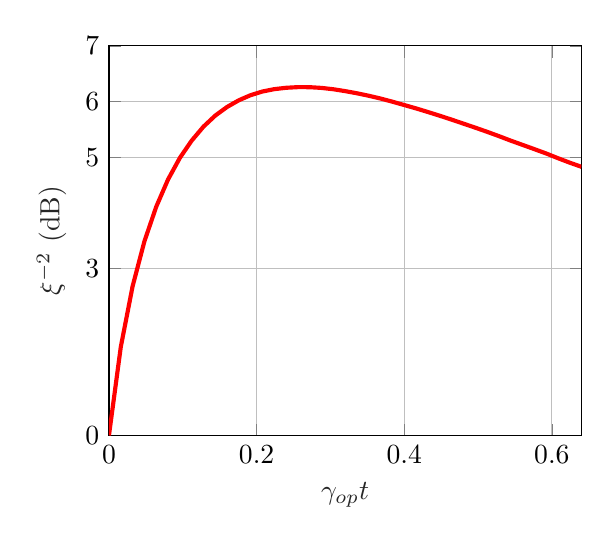
\begin{tikzpicture}

\begin{axis}[%
width=6cm,
height=4.948cm,
at={(0cm,0cm)},
scale only axis,
xmin=0.0000,
xmax=0.6400,
xlabel style={font=\color{white!15!black}},
xlabel={$\gamma_{op}t$},
ymin=0.0000,
ymax=7.0000,
ytick={0.0000,3.0000,5.0000,6.0000,7.0000,8.0000},
ylabel style={font=\color{white!15!black}},
ylabel={$\xi^{-2}$ (dB)},
axis background/.style={fill=white},
xmajorgrids,
ymajorgrids
]
\addplot [color=red, line width=1.5pt, forget plot]
  table[row sep=crcr]{%
0.0000	-0.0000\\
0.0160	1.5869\\
0.0320	2.6777\\
0.0480	3.4854\\
0.0640	4.1073\\
0.0800	4.5969\\
0.0960	4.9858\\
0.1120	5.2951\\
0.1280	5.5470\\
0.1440	5.7463\\
0.1600	5.9008\\
0.1760	6.0219\\
0.1920	6.1135\\
0.2080	6.1792\\
0.2240	6.2214\\
0.2400	6.2458\\
0.2560	6.2575\\
0.2720	6.2565\\
0.2880	6.2434\\
0.3040	6.2194\\
0.3200	6.1858\\
0.3360	6.1468\\
0.3520	6.1025\\
0.3680	6.0522\\
0.3840	5.9960\\
0.4160	5.8755\\
0.4320	5.8107\\
0.4480	5.7440\\
0.4640	5.6746\\
0.4960	5.5304\\
0.5121	5.4557\\
0.5281	5.3781\\
0.5441	5.2971\\
0.5761	5.1444\\
0.5921	5.0664\\
0.6081	4.9818\\
0.6241	4.9007\\
0.6401	4.8260\\
};
\end{axis}
\end{tikzpicture}%
    \label{fig:nanofiber_xi_t_rp1d8a_NA2500}
    }
    \hfill
  \subfloat[h][$ \xi^{-2}_{peak,nanofiber}(N_A) $]{
      %\setlength\figureheight{0.3\textwidth}
      %\setlength\figurewidth{0.3\textwidth}
      \label{fig:nanofiber_peakxi_NA_rp1d8a}
      % This file was created by matlab2tikz.
%
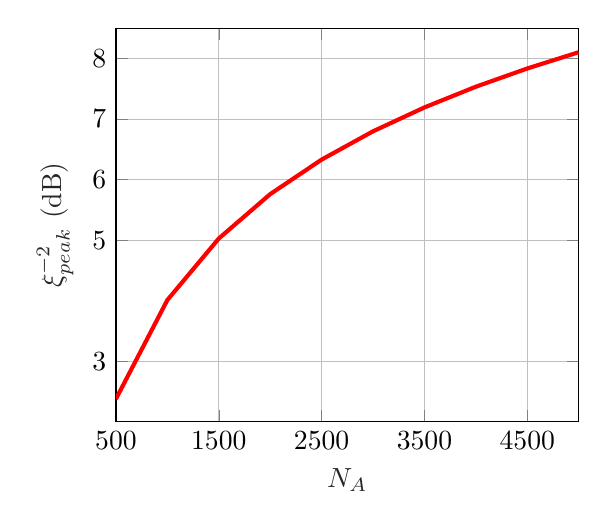
\begin{tikzpicture}

\begin{axis}[%
width=5.877cm,
height=5cm,
at={(0cm,0cm)},
scale only axis,
xmin=500.0000,
xmax=5000.0000,
xtick={500.0000,1500.0000,2500.0000,3500.0000,4500.0000},
xlabel style={font=\color{white!15!black}},
xlabel={$N_A$},
ymin=2.0000,
ymax=8.5000,
ytick={3.0000,5.0000,6.0000,7.0000,8.0000},
ylabel style={font=\color{white!15!black}},
ylabel={$\xi^{-2}_{peak}$ (dB)},
axis background/.style={fill=white},
xmajorgrids,
ymajorgrids
]
\addplot [color=red, line width=1.5pt, forget plot]
  table[row sep=crcr]{%
500.0000	2.3793\\
1000.0000	4.0121\\
1500.0000	5.0278\\
2000.0000	5.7605\\
2500.0000	6.3307\\
3000.0000	6.7978\\
3500.0000	7.1922\\
4000.0000	7.5342\\
4500.0000	7.8352\\
5000.0000	8.1036\\
};
\end{axis}
\end{tikzpicture}%
      }
   \end{minipage}\vfill
   \begin{minipage}[h]{0.95\linewidth}
    %\begin{tabular}{*{2}{b{0.2\textwidth-2\tabcolsep}}}
     \subfloat[h][$\xi^{-2}_{swg}(t)$]{
       %\setlength\figureheight{0.3\textwidth}
       %\setlength\figurewidth{0.3\textwidth}
       % This file was created by matlab2tikz.
%
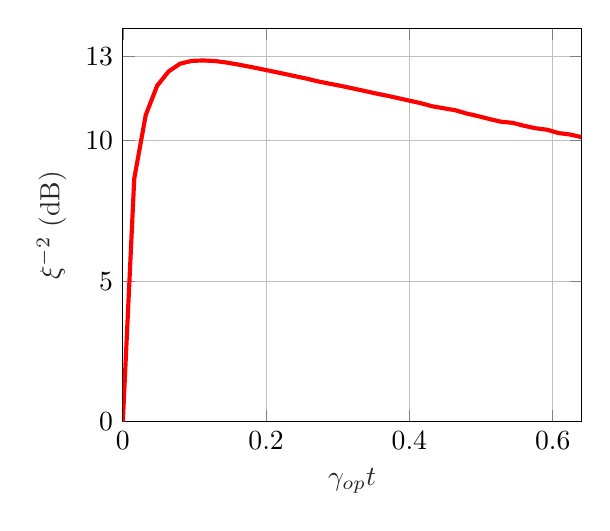
\begin{tikzpicture}

\begin{axis}[%
width=5.824cm,
height=5cm,
at={(0cm,0cm)},
scale only axis,
xmin=0.0000,
xmax=0.6400,
xlabel style={font=\color{white!15!black}},
xlabel={$\gamma_{op}t$},
ymin=-0.0000,
ymax=14.0000,
ytick={0.0000,5.0000,10.0000,13.0000,15.0000},
ylabel style={font=\color{white!15!black}},
ylabel={$\xi^{-2}$ (dB)},
axis background/.style={fill=white},
xmajorgrids,
ymajorgrids
]
\addplot [color=red, line width=1.5pt, forget plot]
  table[row sep=crcr]{%
0.0000	-0.0000\\
0.0160	8.6563\\
0.0320	10.9109\\
0.0480	11.9581\\
0.0640	12.4658\\
0.0800	12.7374\\
0.0960	12.8376\\
0.1120	12.8533\\
0.1280	12.8352\\
0.1440	12.7824\\
0.1600	12.7130\\
0.1760	12.6353\\
0.1920	12.5544\\
0.2240	12.3843\\
0.2400	12.2958\\
0.2560	12.2104\\
0.2720	12.1125\\
0.2880	12.0292\\
0.3040	11.9522\\
0.3360	11.7773\\
0.3520	11.6864\\
0.3680	11.6042\\
0.3840	11.5158\\
0.4000	11.4238\\
0.4160	11.3344\\
0.4320	11.2227\\
0.4640	11.0837\\
0.4800	10.9656\\
0.4960	10.8740\\
0.5121	10.7681\\
0.5281	10.6746\\
0.5441	10.6347\\
0.5601	10.5300\\
0.5761	10.4430\\
0.5921	10.3904\\
0.6081	10.2727\\
0.6241	10.2206\\
0.6401	10.1278\\
};
\end{axis}
\end{tikzpicture}%
       \label{fig:swg_xi_t_rp1d_NA2500}
       }
       \hfill
     \subfloat[h][$ \xi^{-2}_{peak,swg}(N_A) $]{
         %\setlength\figureheight{0.3\textwidth}
         %\setlength\figurewidth{0.3\textwidth}
         \label{fig:swg_peakxi_NA_rp1d}
         % This file was created by matlab2tikz.
%
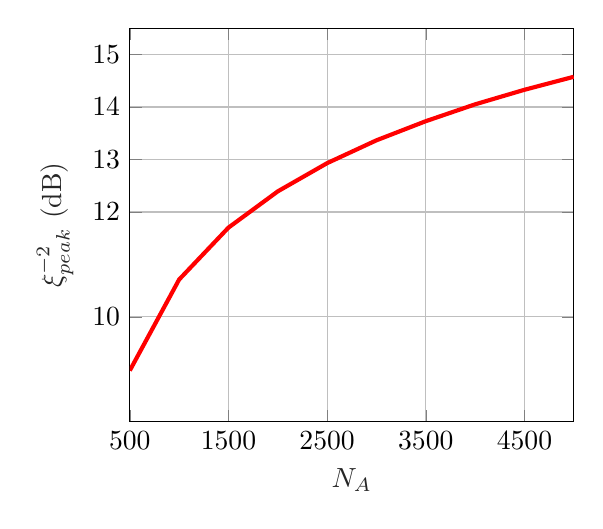
\begin{tikzpicture}

\begin{axis}[%
width=5.639cm,
height=5cm,
at={(0cm,0cm)},
scale only axis,
xmin=500.0000,
xmax=5000.0000,
xtick={500.0000,1500.0000,2500.0000,3500.0000,4500.0000},
xlabel style={font=\color{white!15!black}},
xlabel={$N_A$},
ymin=8.0000,
ymax=15.5000,
ytick={10.0000,12.0000,13.0000,14.0000,15.0000},
ylabel style={font=\color{white!15!black}},
ylabel={$\xi^{-2}_{peak}$ (dB)},
axis background/.style={fill=white},
xmajorgrids,
ymajorgrids
]
\addplot [color=red, line width=1.5pt, forget plot]
  table[row sep=crcr]{%
500.0000	8.9784\\
1000.0000	10.7121\\
1500.0000	11.7014\\
2000.0000	12.3921\\
2500.0000	12.9296\\
3000.0000	13.3648\\
3500.0000	13.7291\\
4000.0000	14.0500\\
4500.0000	14.3273\\
5000.0000	14.5751\\
};
\end{axis}
\end{tikzpicture}%
         }
   \end{minipage}
   %\end{tabular}
\caption{Spin squeezing parameter as a function of time and atom number.}\label{fig:xi_rpfix_NA_t}
\end{figure}

\newpage
\begin{figure}[htb]
\centering
%\pgfplotsset{yticklabel style={text width=3em,align=right}}
 \begin{minipage}[h]{0.95\linewidth}
 %\begin{tabular}{*{2}{b{0.2\textwidth-2\tabcolsep}}}
  \subfloat[h][$\xi^{-2}_{peak,nanofiber}(r\!_\perp)$]{
    %\setlength\figureheight{0.3\textwidth}
    %\setlength\figurewidth{0.3\textwidth}
    % This file was created by matlab2tikz.
%
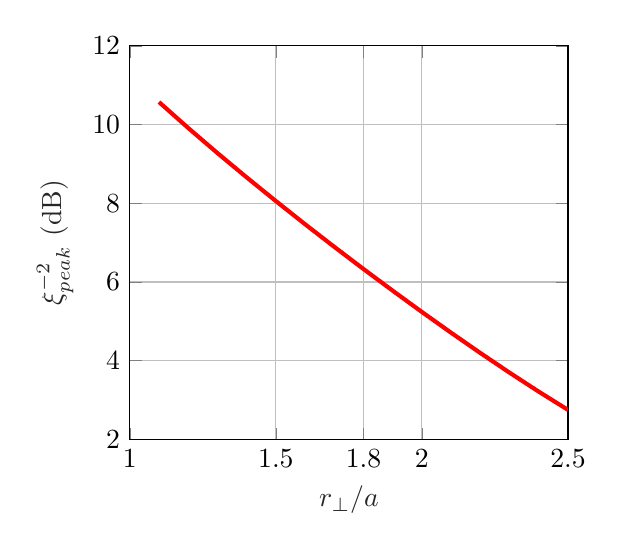
\begin{tikzpicture}

\begin{axis}[%
width=5.565cm,
height=5cm,
at={(0cm,0cm)},
scale only axis,
xmin=1.0000,
xmax=2.5000,
xtick={1.0000,1.5000,1.8000,2.0000,2.5000},
xlabel style={font=\color{white!15!black}},
xlabel={$r_\perp/a$},
ymin=2.0000,
ymax=12.0000,
ylabel style={font=\color{white!15!black}},
ylabel={$\xi^{-2}_{peak}$ (dB)},
axis background/.style={fill=white},
xmajorgrids,
ymajorgrids
]
\addplot [color=red, line width=1.5pt, forget plot]
  table[row sep=crcr]{%
1.1000	10.5712\\
1.2000	9.9128\\
1.3000	9.2762\\
1.4000	8.6588\\
1.5000	8.0571\\
1.6000	7.4685\\
1.7000	6.8935\\
1.8000	6.3307\\
1.9000	5.7799\\
2.0000	5.2394\\
2.1000	4.7118\\
2.2000	4.1974\\
2.3000	3.6980\\
2.4000	3.2157\\
2.5000	2.7531\\
};
\end{axis}
\end{tikzpicture}%
    \label{fig:nanofiber_peakxi_rp_NA2500}
    }
    \hfill
  \subfloat[h][$ C_1(r\!_\perp) $ of a nanofiber]{
      %\setlength\figureheight{0.3\textwidth}
      %\setlength\figurewidth{0.3\textwidth}
      \label{fig:nanofiber_C1_y}
      % This file was created by matlab2tikz.
%
%The latest updates can be retrieved from
%  http://www.mathworks.com/matlabcentral/fileexchange/22022-matlab2tikz-matlab2tikz
%where you can also make suggestions and rate matlab2tikz.
%
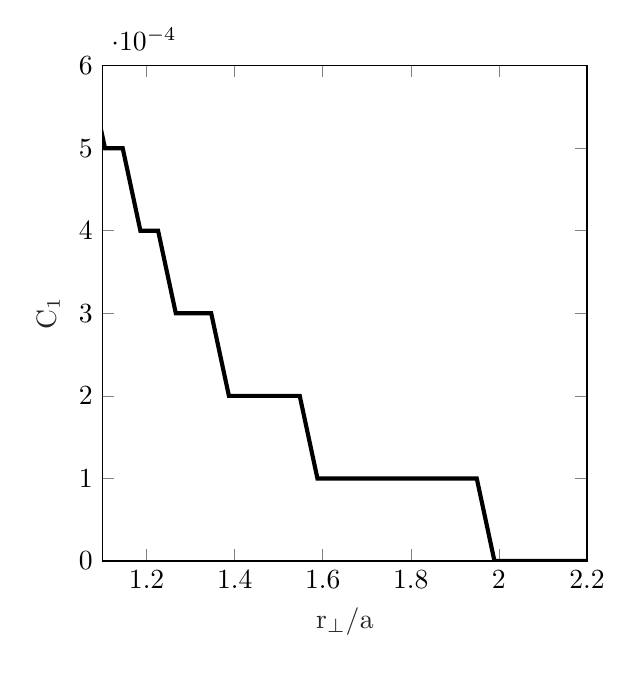
\begin{tikzpicture}

\begin{axis}[%
width=2.422in,
height=2.477in,
at={(0.406in,0.413in)},
scale only axis,
xmin=1.1000,
xmax=2.2000,
xlabel style={font=\color{white!15!black}},
xlabel={$\text{r}_\perp\text{/a}$},
ymin=0.0000,
ymax=0.0006,
ylabel style={font=\color{white!15!black}},
ylabel={$\text{C}_\text{1}$},
axis background/.style={fill=white}
]
\addplot [color=black, line width=1.5pt, forget plot]
  table[row sep=crcr]{%
1.0653	0.0006\\
1.1055	0.0005\\
1.1457	0.0005\\
1.1859	0.0004\\
1.2261	0.0004\\
1.2663	0.0003\\
1.3065	0.0003\\
1.3467	0.0003\\
1.3869	0.0002\\
1.4271	0.0002\\
1.4673	0.0002\\
1.5075	0.0002\\
1.5477	0.0002\\
1.5879	0.0001\\
1.6281	0.0001\\
1.6683	0.0001\\
1.7085	0.0001\\
1.7487	0.0001\\
1.7889	0.0001\\
1.8291	0.0001\\
1.8693	0.0001\\
1.9095	0.0001\\
1.9497	0.0001\\
1.9899	0.0000\\
2.0302	0.0000\\
2.0704	0.0000\\
2.1106	0.0000\\
2.1508	0.0000\\
2.2312	0.0000\\
};
\end{axis}
\end{tikzpicture}%
      }
   \end{minipage}\vfill
   \begin{minipage}[h]{0.95\linewidth}
    %\begin{tabular}{*{2}{b{0.2\textwidth-2\tabcolsep}}}
     \subfloat[h][$\xi^{-2}_{peak,swg}(r\!_\perp)$]{
       %\setlength\figureheight{0.3\textwidth}
       %\setlength\figurewidth{0.3\textwidth}
       % This file was created by matlab2tikz.
%
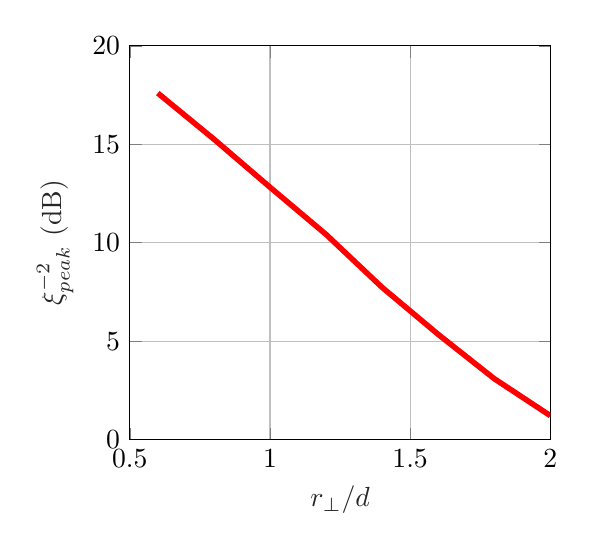
\begin{tikzpicture}

\begin{axis}[%
width=5.341cm,
height=5cm,
at={(0cm,0cm)},
scale only axis,
xmin=0.5000,
xmax=2.0000,
xtick={0.5000,1.0000,1.5000,2.0000},
xlabel style={font=\color{white!15!black}},
xlabel={$r_\perp/d$},
ymin=0.0000,
ymax=20.0000,
ylabel style={font=\color{white!15!black}},
ylabel={$\xi^{-2}_{peak}$ (dB)},
axis background/.style={fill=white},
xmajorgrids,
ymajorgrids
]
\addplot [color=red, line width=2.0pt, forget plot]
  table[row sep=crcr]{%
0.6000	17.5969\\
0.8000	15.2582\\
1.0000	12.8169\\
1.2000	10.4185\\
1.4000	7.7272\\
1.6000	5.3402\\
1.8000	3.0891\\
2.0000	1.2100\\
};
\end{axis}
\end{tikzpicture}%
       \label{fig:swg_peakxi_rp_NA2500}
       }
       \hfill
     \subfloat[h][$ C_1(r\!_\perp) $ of a SWG]{
         %\setlength\figureheight{0.3\textwidth}
         %\setlength\figurewidth{0.3\textwidth}
         \label{fig:swg_C1_y}
         % This file was created by matlab2tikz.
%
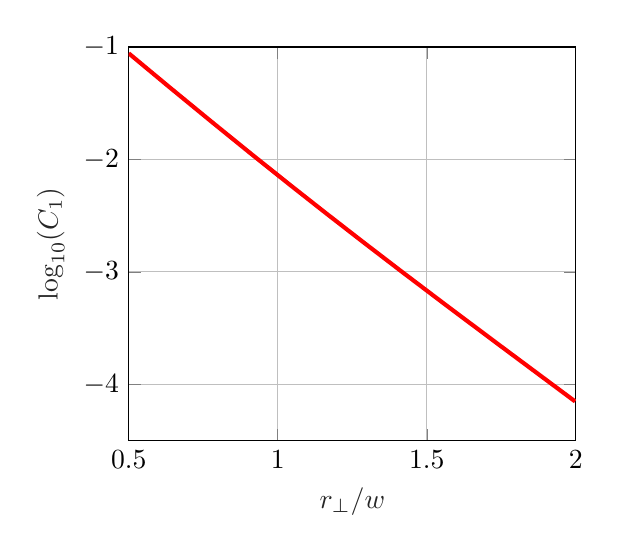
\begin{tikzpicture}

\begin{axis}[%
width=5.679cm,
height=5cm,
at={(0cm,0cm)},
scale only axis,
xmin=0.5000,
xmax=2.0000,
xlabel style={font=\color{white!15!black}},
xlabel={$r_\perp/w$},
ymin=-4.5000,
ymax=-1.0000,
ylabel style={font=\color{white!15!black}},
ylabel={$\log_{10}(C_1)$},
axis background/.style={fill=white},
xmajorgrids,
ymajorgrids
]
\addplot [color=red, line width=1.5pt, forget plot]
  table[row sep=crcr]{%
0.5000	-1.0564\\
0.6343	-1.3523\\
0.7786	-1.6662\\
0.9129	-1.9548\\
1.0373	-2.2182\\
1.1617	-2.4778\\
1.2861	-2.7338\\
1.4204	-3.0065\\
1.5697	-3.3058\\
1.7438	-3.6511\\
1.9975	-4.1513\\
};
\end{axis}
\end{tikzpicture}%
         }
   \end{minipage}
   %\end{tabular}
\caption{Peak squeezing parameter and cooperativity as a function of atom position.}\label{fig:peakxi_rp_NA}
\end{figure}


%====== SECTION: Summary and outlook ======%
\section{Summary and Outlook} \label{Sec::Conclusion}


ACKNOWLEDGMENTS
We thank the UNM Center for Advanced Research Computing for computational resources used in this work.
This work was supported by the NSF, under grants PHY-1212445, xxxxx.

\bibliography{refs/Archive}


%=========== APPENDIX ===========%
\begin{appendix}

%===================APPENDIX: Hamiltonian =====================%
\section{Faraday interaction Hamiltonian} \label{Appendix::FaradayInteractionHamiltonian}
In the Faraday interaction spin squeezing protocol, we define the fiducial, coupled and transfer states by $ \ket{\uparrow}=\ket{f=4,f_x=4} $, $ \ket{\downarrow}=\ket{f=4,f_x=3} $ and $ \ket{T}=\ket{f=4,f_x=2} $ respectively in the $ x $-basis. 
A set of spin operators projected onto the truncated qutrit subspace spanned by these three basis states can be defined by
\begin{align}
\hat{f_x} &= -f \ket{\uparrow}\bra{\uparrow} -(f-1)\ket{\downarrow}\bra{\downarrow}-(f-2)\ket{T}\bra{T},\\
\hat{f_y} &=i\left[\sqrt{\frac{f}{2}}\left(\ket{\downarrow}\bra{\uparrow}-\ket{\uparrow}\bra{\downarrow}\right) +\sqrt{\frac{2f-1}{2}}\left(\ket{T}\bra{\downarrow}-\ket{\downarrow}\bra{T} \right) \right] ,\\
\hat{f_z} &= \sqrt{\frac{f}{2}}\left(\ket{\downarrow}\bra{\uparrow}+\ket{\uparrow}\bra{\downarrow}\right) +\sqrt{\frac{2f-1}{2}}\left(\ket{T}\bra{\downarrow}+\ket{\downarrow}\bra{T} \right).
\end{align}

We also define a set of Stokes operators as below,
\begin{align}
\hat{S}_0 &= \smallfrac{1}{2}\big[ \hat{a}^\dag_H(t) \hat{a}_H(t)+\hat{a}^\dag_V(t) \hat{a}_V(t) \big],\\
\hat{S}_1 &= \smallfrac{1}{2}\big[ \hat{a}^\dag_H(t) \hat{a}_H(t)-\hat{a}^\dag_V(t) \hat{a}_V(t) \big],\\
\hat{S}_2 &= \smallfrac{1}{2}\big[ \hat{a}^\dag_H(t) \hat{a}_V(t)+\hat{a}^\dag_V(t) \hat{a}_H(t) \big],\\
\hat{S}_3 &= \smallfrac{1}{2i}\big[ \hat{a}^\dag_H(t) \hat{a}_V(t) -\hat{a}^\dag_V(t) \hat{a}_H(t) \big],
\end{align}
where the photon annihilation operators of the horizontally and vertically polarized modes denoted with subscription $ H $ and $ V $ respectively are related to the left- and right-circularly polarized modes denoted with subscription $ L $ and $ R $ by $ \hat{a}_{H}=(\hat{a}_L+\hat{a}_R) /\sqrt{2}$ and $ \hat{a}_{V}=i(\hat{a}_R-\hat{a}_L)/\sqrt{2} $.
The local quasimonochromatic electric field operator at $\br= (r\!_\perp,\phi,z) $ with a set of degenerate guided modes at frequency $ \omega_0 $ and propagating in the group velocity of $ v_g $ can be given by
\begin{align}\label{eq:Ebp}
\hat{\mathbf{E}}^{(+)}(r\!_\perp,\phi,z;t) &= \sum_{b,p} \sqrt{ \frac{2 \pi \hbar \omega_0}{ v_g} } \mathbf{u}_{b,p}(r\!_\perp,\phi) \hat{a}_{b,p}(z,t)  e^{i (b\beta_0 z- \omega_0 t)},
\end{align}
where $ b $ is the sign of the propagation direction and $ p $ is the polarization label of the orthonormal modes.
In our case, we only have forward propagating modes for the QND measurement protocols, and hence we will only have $ b=+ $.

\comment{Todo: Rewrite the effective Hamiltonian using the collective operators defined above.}

%===================APPENDIX: Circular VS linear polarization mode bases =====================%
\section{Circular V.S. linear polarization bases}\label{Appendix:LRbases}
\comment{This content is mainly typed from my notes on Faraday Interaction in The Nanofiber Geometry. More can be done here, including a generalization of polarization transformation using $ \mathbf{SU}(2) $ group generators.}

In this section, we will derive the equations of Stokes vector operators and spin-polarization interaction Hamiltonian due to polarization basis transformations.
A general basis transformation theory will be derived in the context of linear-polarization basis transformations, and will then be applied to the linear $ D/\bar{D} $- and circular $ R/L $-bases cases.

\subsection{Spin-polarization Hamiltonian and Stokes vector operators in a linear basis}
In general, we can define an arbitrary linear polarization basis by
\begin{align}
\left(\!\begin{array}{c}
\mathbf{e}_n \\ \mathbf{e}_{\bar{n}}
\end{array}\!\right) &= 
\left(\!\!\begin{array}{cc}
\cos\theta & \sin\theta \\
- \sin\theta & \cos\theta
\end{array}\!\!\right)\bullet
\left(\!\begin{array}{c}
\mathbf{e}_H \\ \mathbf{e}_V
\end{array}\!\right)
=\mathbf{R}(\theta)\bullet \left(\!\begin{array}{c}
\mathbf{e}_H \\ \mathbf{e}_V
\end{array}\!\right),
\end{align}
or the inversed relationship
\begin{align}
\left(\!\begin{array}{c}\mathbf{e}_H \\ \mathbf{e}_V\end{array}\!\right)&= \mathbf{R}^{-1}(\theta)\bullet\left(\!\begin{array}{c}\mathbf{e}_n \\ \mathbf{e}_{\bar{n}}\end{array}\!\right),
\end{align}
where $ \theta $ is the angle of the $ \mathbf{e}_n $ basis rotated from the $ H $-direction around $ z $-axis, and $ \mathbf{e}_{\bar{n}} $ is the basis vector $ 90^\circ $ from the $ \mathbf{e}_n $ direction; $ \mathbf{R}(\theta)=\mathbf{R}_z(\theta) $ is the Euler rotation matrix about the $ z $-axis by $ \theta $ in the real-number $ \mathbf{SO}(3) $ rotation group, which has the property that $ \mathbf{R}^{-1}(\theta)=\mathbf{R}^T(\theta)=\mathbf{R}(-\theta) $. 
More generally, the basis transformation matrix is an unitary matrix determined by two parameters (two degrees of freedom)--$ \theta $ and $ \phi $--corresponding to the rotating angles around one axis and an relative phase between the base components, which is in the $ \mathbf{SU}(2) $ group.
%We denote the general case with $ \mathbf{R}=\mathbf{R}(\theta,\phi) $, or in the form of two-step rotations around $ i $-axis and then around $ j $-axis by $ \mathbf{R}=\mathbf{R}_j(\theta)\mathbf{R}_i(\phi) $, always satisfying $ \mathbf{R}^{-1}=\mathbf{R}^\dagger $ for either rotations.

Not to be confused, we have also defined an operator space spanned by operator vectors, like $ \left(\!\begin{array}{cc}\mathbf{e}_n,&\mathbf{e}_{\bar{n}}\end{array}\! \right) $, which has vectors, tensors or operators as the elements.
We have also defined the bullet operator ($ \bullet $) in the operator vector space isomorphically the same as the dot ($ \cdot $) product or matrix product in the conventional vector space while the sign of $ \cdot $ can usually be ignored and we will denote complex conjugates explicitly if needed. 
$ \mathbf{R}(\theta) $ and its transformations is a tensor defined in the operator vector space as well.
When a conventional vector or tensor multiplies with an operator vector or tensor, we will use $ \cdot $ between them and the conventional vector or tensor will be formally treated as a scalar to be $ \cdot $ multiplied with the elements of the operator vector or tensor. 
Two operator vectors in a $ \bullet $ multiplication form a mutual covariant relationship in the operator space.
 
With the coordinate basis rotated passively, both the mode components and the field annihilation operators should be rotated actively by $ -\theta $ to be transformation-equivalent.
Written in the matrix form in the operator space, 
\begin{align}
\left(\!\begin{array}{c}\mathbf{u}_n \\ \mathbf{u}_{\bar{n}}\end{array}\!\right) &= \mathbf{R}^{-1}(\theta)\bullet\left(\!\begin{array}{c}\mathbf{u}_H \\ \mathbf{u}_V\end{array}\!\right)\\
\hat{\mathbf{a}}_{n,\bar{n}} &=\mathbf{R}^{-1}(\theta)\bullet \hat{\mathbf{a}}_{H,V},
\end{align}
where $ \hat{\mathbf{a}}_{n,\bar{n}}=[\hat{a}_n;\hat{a}_{\bar{n}}] $ and $ \hat{\mathbf{a}}_{H,V}=[\hat{a}_H;\hat{a}_V] $ are the annihilation operator vectors using the $ \{n,\bar{n} \} $ and $ \{H,V \} $ bases, respectively.
In our notation, we use $ [\cdot ;\cdots] $ notation to indicate $ 1\times n $ vectors as general matrices.

Using the definition in the $ \{ H,V\} $-basis of the Stokes operators (Eq.\eqref{eq:SaHVaRL}) and the annihilation operator basis transformation relationships above, one can rewrite the Stokes operators in the $ \{\mathbf{e}_n, \mathbf{e}_{\bar{n}}\} $ basis by
\begin{subequations}\label{eq:Snnbar}
\begin{align}
\hat{S}_0 &= \frac{1}{2}\left[\left(\!\begin{array}{cc}\hat{a}_n^\dagger,& \hat{a}_{\bar{n}}^\dagger\end{array} \!\right)\bullet\mathbf{R}_{[1,:]}^\dagger(\theta)\bullet\mathbf{R}_{[1,:]}(\theta)\bullet
\left(\!\begin{array}{c}\hat{a}_n\\ \hat{a}_{\bar{n}}\end{array} \!\right)
+ \left(\!\begin{array}{cc}\hat{a}_n^\dagger,& \hat{a}_{\bar{n}}^\dagger\end{array} \!\right)\bullet\mathbf{R}^\dagger_{[2,:]}(\theta)\bullet\mathbf{R}_{[2,:]}(\theta)\bullet
\left(\!\begin{array}{c}\hat{a}_n\\ \hat{a}_{\bar{n}}\end{array} \!\right) \right]\nn\\
&= \frac{1}{2}\left\{\left(\!\begin{array}{cc}\hat{a}_n^\dagger,& \hat{a}_{\bar{n}}^\dagger\end{array} \!\right)\bullet
\left[\left(\!\begin{array}{cc}\cos^2\theta,& \frac{1}{2}\sin 2\theta \\ \frac{1}{2}\sin 2\theta, & \sin^2\theta\end{array} \!\right)
+ \left(\!\begin{array}{cc}\sin^2\theta,& -\frac{1}{2}\sin 2\theta \\ -\frac{1}{2}\sin 2\theta, & \cos^2\theta\end{array} \!\right)\right]\bullet
\left(\!\begin{array}{c}\hat{a}_n\\ \hat{a}_{\bar{n}}\end{array} \!\right)\right\}\nn\\
&=\frac{1}{2} \left[\hat{a}_n^\dagger\hat{a}_n+\hat{a}_{\bar{n}}^\dagger\hat{a}_{\bar{n}} \right]\\
\hat{S}_1 &= \frac{1}{2}\left\{\left(\!\begin{array}{cc}\hat{a}_n^\dagger,& \hat{a}_{\bar{n}}^\dagger\end{array} \!\right)
\bullet\left[\mathbf{R}_{[1,:]}^\dagger(\theta)\bullet\mathbf{R}_{[1,:]}(\theta) - \mathbf{R}_{[2,:]}^\dagger(\theta)\bullet\mathbf{R}_{[2,:]}(\theta) \right]
\bullet\left(\!\begin{array}{c}\hat{a}_n\\ \hat{a}_{\bar{n}}\end{array} \!\right) \right\}\nn\\
&= \frac{1}{2} \left[\cos 2\theta \hat{a}_n^\dagger\hat{a}_n + \sin 2\theta \hat{a}_n^\dagger\hat{a}_{\bar{n}} + \sin 2\theta \hat{a}_{\bar{n}}^\dagger\hat{a}_n -\cos 2\theta \hat{a}_{\bar{n}}^\dagger\hat{a}_{\bar{n}} \right]\\
\hat{S}_2 &= \frac{1}{2}\left\{\left(\!\begin{array}{cc}\hat{a}_n^\dagger,& \hat{a}_{\bar{n}}^\dagger\end{array} \!\right)
\bullet\left[\mathbf{R}_{[1,:]}^\dagger(\theta)\bullet\mathbf{R}_{[2,:]}(\theta) + \mathbf{R}_{[2,:]}^\dagger(\theta)\bullet\mathbf{R}_{[1,:]}(\theta) \right]
\bullet\left(\!\begin{array}{c}\hat{a}_n\\ \hat{a}_{\bar{n}}\end{array} \!\right) \right\}\nn\\
&= \frac{1}{2} \left[-\sin 2\theta \hat{a}_n^\dagger\hat{a}_n + \cos 2\theta \hat{a}_n^\dagger\hat{a}_{\bar{n}} + \cos 2\theta \hat{a}_{\bar{n}}^\dagger\hat{a}_n +\sin 2\theta \hat{a}_{\bar{n}}^\dagger\hat{a}_{\bar{n}} \right]\\
\hat{S}_3 &= \frac{1}{2i}\left\{\left(\!\begin{array}{cc}\hat{a}_n^\dagger,& \hat{a}_{\bar{n}}^\dagger\end{array} \!\right)
\bullet\left[\mathbf{R}_{[1,:]}^\dagger(\theta)\bullet\mathbf{R}_{[2,:]}(\theta) - \mathbf{R}_{[2,:]}^\dagger(\theta)\bullet\mathbf{R}_{[1,:]}(\theta) \right]
\bullet\left(\!\begin{array}{c}\hat{a}_n\\ \hat{a}_{\bar{n}}\end{array} \!\right) \right\}\nn\\
&= \frac{1}{2i} \left[\hat{a}_n^\dagger\hat{a}_{\bar{n}} - \hat{a}_{\bar{n}}^\dagger\hat{a}_n  \right].
\end{align}
\end{subequations}
In deriving the equations above, we have denoted $ \mathbf{R}_{[i,:]}(\theta) $ as the $ i $-th row of $ \mathbf{R}(\theta) $ and $ \mathbf{R}_{[i,:]}^\dagger(\theta) $ as the conjugate transpose of the $ i $-th row of $ \mathbf{R}(\theta) $.
As a shorthand, these relationships of Stokes operators can be expressed as an operator transformation, $ \hat{\mathbf{S}}=\mathbf{M}\bullet\hat{\mathbf{A}}_{n,\bar{n}} $, where $ \hat{\mathbf{S}}=[\hat{S}_0;\hat{S}_1;\hat{S}_2;\hat{S}_3] $ and $ \hat{\mathbf{A}}_{n,\bar{n}}=[\hat{a}_n^\dagger\hat{a}_n;\hat{a}_n^\dagger\hat{a}_{\bar{n}};\hat{a}_{\bar{n}}^\dagger\hat{a}_n;\hat{a}_{\bar{n}}^\dagger\hat{a}_{\bar{n}}] $ are the operator vectors and $ \mathbf{M} $ is the transformation matrix defined by the transformation coefficients in Eqs.\eqref{eq:Snnbar}.
One can prove that the inversed transformation matrix $ \mathbf{M}^{-1}=2\mathbf{M}^\dagger $, and $ \mathbf{M} $ can be derived in the following form, in general,
\begin{align}
\mathbf{M} &=\frac{1}{2}\left(\!\begin{array}{c}
\mathrm{vec}_r\left[\mathbf{R}_{[1,:]}^\dagger(\theta)\mathbf{R}_{[1,:]}(\theta) + \mathbf{R}_{[2,:]}^\dagger(\theta)\mathbf{R}_{[2,:]}(\theta) \right]\\
\mathrm{vec}_r\left[\mathbf{R}_{[1,:]}^\dagger(\theta)\mathbf{R}_{[1,:]}(\theta) - \mathbf{R}_{[2,:]}^\dagger(\theta)\mathbf{R}_{[2,:]}(\theta) \right]\\
\mathrm{vec}_r\left[\mathbf{R}_{[1,:]}^\dagger(\theta)\mathbf{R}_{[2,:]}(\theta) + \mathbf{R}_{[2,:]}^\dagger(\theta)\mathbf{R}_{[1,:]}(\theta) \right]\\
-i\mathrm{vec}_r\left[\mathbf{R}_{[1,:]}^\dagger(\theta)\mathbf{R}_{[2,:]}(\theta) - \mathbf{R}_{[2,:]}^\dagger(\theta)\mathbf{R}_{[1,:]}(\theta) \right]
 \end{array} \!\right)\\
&= \frac{1}{2}\left(\!\begin{array}{cccc} 1,&0,&0,& 1\\
\cos 2\theta,&\sin 2\theta, & \sin 2\theta, & -\cos 2\theta\\
-\sin 2\theta, & \cos 2\theta, & \cos 2\theta, & \sin 2\theta\\
0,&-i,& i,& 0\end{array}\!\right),
\end{align}
where $ \mathrm{vec}_r[\cdot] $ means the vectorization of a matrix by concatenating its rows. 


By using the vector space representation, the E-field operator can be written in the $ \{n,\bar{n}\} $ basis by 
\begin{align}
\hat{\mathbf{E}}^{(+)}(\br;t) &= \sqrt{ \frac{2 \pi \hbar \omega_0}{ v_g} } \left[\mathbf{u}_H(r\!_\perp,\phi) \hat{a}_H(z,t) + \mathbf{u}_V(r\!_\perp,\phi) \hat{a}_V(z,t)\right]  e^{i (\beta_0 z- \omega_0 t)}\\
&= \sqrt{ \frac{2 \pi \hbar \omega_0}{ v_g} } \left(\!\begin{array}{cc}\mathbf{u}_H, & \mathbf{u}_V\end{array}\!\right)
\bullet \left(\!\begin{array}{c}\hat{a}_H\\ \hat{a}_V\end{array} \!\right)  e^{i (\beta_0 z- \omega_0 t)}\\
&= \sqrt{ \frac{2 \pi \hbar \omega_0}{ v_g} } \left(\!\begin{array}{cc}\mathbf{u}_H, & \mathbf{u}_V\end{array}\!\right)\bullet\mathbf{R}(\theta)
\bullet \mathbf{R}^{-1}(\theta)\bullet\left(\!\begin{array}{c}\hat{a}_H\\ \hat{a}_V\end{array} \!\right)  e^{i (\beta_0 z- \omega_0 t)}\\
&= \sqrt{ \frac{2 \pi \hbar \omega_0}{ v_g} } \left(\!\begin{array}{cc}\mathbf{u}_n, & \mathbf{u}_{\bar{n}}\end{array}\!\right)
\bullet \left(\!\begin{array}{c}\hat{a}_n\\ \hat{a}_{\bar{n}}\end{array} \!\right)  e^{i (\beta_0 z- \omega_0 t)}\\
&= \sqrt{ \frac{2 \pi \hbar \omega_0}{ v_g} } \left[\mathbf{u}_n(r\!_\perp,\phi) \hat{a}_n(z,t) + \mathbf{u}_{\bar{n}}(r\!_\perp,\phi) \hat{a}_{\bar{n}}(z,t)\right]  e^{i (\beta_0 z- \omega_0 t)}.\label{eq:Efieldop_nnbar}
\end{align}
As expected, the field operator preserves the form in the new basis as defined in Eq.\eqref{eq:Ebp}.

Therefore, the effective atom-light interaction Hamiltonian can be written as
\begin{align}
\hat{h}_\eff &= -\hat{\mathbf{E}}^{(-)}(\br')\cdot\hat{\tensor{\mathbf{\alpha}}}\cdot\hat{\mathbf{E}}^{(+)}(\br')\nn\\
&=-\frac{2 \pi \hbar \omega_0}{ v_g}
\left(\!\begin{array}{cc}\hat{a}_n^\dagger, & \hat{a}_{\bar{n}}^\dagger\end{array} \!\right)\bullet \left(\!\begin{array}{c}\mathbf{u}_n^*\\ \mathbf{u}_{\bar{n}}^*\end{array}\!\right)
\cdot\hat{\tensor{\mathbf{\alpha}}}\cdot
\left(\!\begin{array}{cc}\mathbf{u}_n, & \mathbf{u}_{\bar{n}}\end{array}\!\right)
\bullet \left(\!\begin{array}{c}\hat{a}_n\\ \hat{a}_{\bar{n}}\end{array} \!\right) \nn\\
&= \hbar \left(\!\begin{array}{cc}\hat{a}_n^\dagger, & \hat{a}_{\bar{n}}^\dagger\end{array} \!\right)\bullet
\left(\!\begin{array}{cc} \hat{\chi}_{nn},&\hat{\chi}_{n\bar{n}}\\
\hat{\chi}_{\bar{n}n},&\hat{\chi}_{\bar{n}\bar{n}}\end{array} \!\right)
\bullet\left(\!\begin{array}{c}\hat{a}_n\\ \hat{a}_{\bar{n}}\end{array} \!\right) \nn\\
&= \hbar \hat{\boldsymbol{\chi}}_{n,\bar{n}}^\dagger\bullet \hat{\mathbf{A}}_{n,\bar{n}}= \hbar \hat{\boldsymbol{\chi}}_{n,\bar{n}}^\dagger\bullet 2\mathbf{M}^\dagger\bullet \hat{\mathbf{S}}\\
&= \hbar\left\{(\hat{\chi}_{nn}+ \hat{\chi}_{\bar{n}\bar{n}})\hat{S}_0 \right.\nn\\
&\quad+ [\cos 2\theta \hat{\chi}_{nn}+ \sin 2\theta(\hat{\chi}_{n\bar{n}}+\hat{\chi}_{\bar{n}n}) - \cos 2\theta\hat{\chi}_{\bar{n}\bar{n}}]\hat{S}_1 \nn\\
&\quad+ [-\sin 2\theta \hat{\chi}_{nn}+ \cos 2\theta(\hat{\chi}_{n\bar{n}}+\hat{\chi}_{\bar{n}n}) + \sin 2\theta \hat{\chi}_{\bar{n}\bar{n}}]\hat{S}_2 \nn\\
&\quad+\left. i \left(\hat{\chi}_{n\bar{n}}-\hat{\chi}_{\bar{n}n}\right)\hat{S}_3 \right\}.\label{eq:heff_nnbarChiS}
\end{align}
In deriving the expression above, we have defined $\hat{\boldsymbol{\chi}}_{n,\bar{n}}=[\hat{\chi}_{nn};\hat{\chi}_{n\bar{n}};\hat{\chi}_{\bar{n}n};\hat{\chi}_{\bar{n}\bar{n}}]$ as the coupling operator vector.
The coupling coefficient elements of $ 2\mathbf{M}^\dagger $, $ 2M_{ij} $, correspond to the coupling coefficients in Eq.\eqref{eq:heff_nnbarChiS} between the spin operators in $ \hat{\boldsymbol{\chi}}_{n,\bar{n}} $ and the polarization operators in $ \hat{\mathbf{S}} $, and each column of $ 2\mathbf{M}^\dagger $ corresponds to the coefficients in the corresponding line of the $ \hat{S}_i $ coupling term in Eq.\eqref{eq:heff_nnbarChiS}.


If we set $ \theta=\pi/4 $, we will be in the $ \{\mathbf{e}_D,\mathbf{e}_{\bar{D}} \} $ basis.
\begin{subequations}
\begin{align}
\hat{a}_D &= \frac{1}{\sqrt{2}}(\hat{a}_H-\hat{a}_V)\\
\hat{a}_{\bar{D}} &= \frac{1}{\sqrt{2}}(\hat{a}_H+\hat{a}_V),
\end{align}
\end{subequations}
or,
\begin{subequations}
\begin{align}
\hat{a}_H &= \frac{1}{\sqrt{2}}(\hat{a}_D+\hat{a}_{\bar{D}})\\
\hat{a}_V &= \frac{1}{\sqrt{2}}(\hat{a}_{\bar{D}}-\hat{a}_D).
\end{align}
\end{subequations}
The Stokes operators becomes
\begin{subequations}
\begin{align}
\hat{S}_0 &= \frac{1}{2} \left[\hat{a}_D^\dagger\hat{a}_D+\hat{a}_{\bar{D}}^\dagger\hat{a}_{\bar{D}} \right]\\
\hat{S}_1 &= \frac{1}{2} \left[ \hat{a}_D^\dagger\hat{a}_{\bar{D}} +  \hat{a}_{\bar{D}}^\dagger\hat{a}_D \right]\\
\hat{S}_2 &= \frac{1}{2} \left[ \hat{a}_{\bar{D}}^\dagger\hat{a}_{\bar{D}}-\hat{a}_D^\dagger\hat{a}_D \right]\\
\hat{S}_3 &= \frac{1}{2i} \left[\hat{a}_D^\dagger\hat{a}_{\bar{D}}-\hat{a}_{\bar{D}}^\dagger\hat{a}_D \right].
\end{align}
\end{subequations}
The field operator becomes 
\begin{align}
\hat{\mathbf{E}}^{(+)}(\br;t) &=\sqrt{ \frac{2 \pi \hbar \omega_0}{ v_g} } \left[\mathbf{u}_D(r\!_\perp,\phi) \hat{a}_D(z,t)+\mathbf{u}_{\bar{D}}(r\!_\perp,\phi) \hat{a}_{\bar{D}}(z,t)  \right]e^{i (\beta_0 z- \omega_0 t)}.
\end{align}
The effective Hamiltonian can be simplified from Eq.\eqref{eq:heff_nnbarChiS} to 
\begin{align}
\hat{h}_\eff &= \hbar[(\hat{\chi}_{DD}+\hat{\chi}_{\bar{D}\bar{D}})\hat{S}_0 +(\hat{\chi}_{D\bar{D}}+\hat{\chi}_{\bar{D}D} )\hat{S}_1\nn\\
&\quad + (\hat{\chi}_{\bar{D}\bar{D}}-\hat{\chi}_{DD})\hat{S}_2 +i(\hat{\chi}_{D\bar{D}}-\hat{\chi}_{\bar{D}D} )\hat{S}_3].
\end{align}
The Hamiltonian expression above should satisfy the cyclical transformation from the $ H $- and $ V $-basis expression.

\subsection{Spin-polarization Hamiltonian and Stokes vector operators in a circular basis}
We define a set of polarization vector transformation relationships by 
\begin{subequations}
\begin{align}
\hat{a}_H &= \frac{1}{\sqrt{2}}(\hat{a}_R+\hat{a}_L )\\
\hat{a}_V &= \frac{i}{\sqrt{2}}(\hat{a}_R-\hat{a}_L ),
\end{align}
\end{subequations}
or the inverse
\begin{subequations}
\begin{align}
\hat{a}_R &= \frac{1}{\sqrt{2}}(\hat{a}_H-i\hat{a}_V )\\
\hat{a}_L &= \frac{1}{\sqrt{2}}(\hat{a}_H+i\hat{a}_V ),
\end{align}
\end{subequations}
where $ R $($ L $) indicates the right(left)-circularly polarized mode.
The Stokes operators can then be defined in both linear ($ H $ and $ V $) and circular ($ L $ and $ R $) polarization bases by
\begin{subequations}\label{eq:SaHVaRL}
\begin{align}
\hat{S}_0 &= \frac{1}{2} \left[\hat{a}_H^\dagger\hat{a}_H+\hat{a}_V^\dagger\hat{a}_V \right] = \frac{1}{2} \left[\hat{a}_R^\dagger\hat{a}_R+\hat{a}_L^\dagger\hat{a}_L \right]\\
\hat{S}_1 &= \frac{1}{2} \left[\hat{a}_H^\dagger\hat{a}_H-\hat{a}_V^\dagger\hat{a}_V \right] = \frac{1}{2} \left[\hat{a}_R^\dagger\hat{a}_L+\hat{a}_L^\dagger\hat{a}_R \right]\\
\hat{S}_2 &= \frac{1}{2} \left[\hat{a}_H^\dagger\hat{a}_V+\hat{a}_V^\dagger\hat{a}_H \right] = \frac{i}{2} \left[\hat{a}_L^\dagger\hat{a}_R-\hat{a}_R^\dagger\hat{a}_L \right]\\
\hat{S}_3 &= \frac{1}{2i} \left[\hat{a}_H^\dagger\hat{a}_V-\hat{a}_V^\dagger\hat{a}_H \right] = \frac{1}{2} \left[\hat{a}_R^\dagger\hat{a}_R-\hat{a}_L^\dagger\hat{a}_L \right].
\end{align}
\end{subequations}
The inversed transformations can be easily derived by inverting the transformation coefficient matrices. 

Based on Eq.\eqref{eq:Ebp}, when the input probe can be decomposed into degenerate orthonormal guided modes in the $H/V $ or $ R/L $ bases, the E-field operator can be written in the quasilinear and quasicircular mode bases by 
\begin{align}
\hat{\mathbf{E}}^{(+)}(r\!_\perp,\phi,z;t) &= \sqrt{ \frac{2 \pi \hbar \omega_0}{ v_g} } \left[\mathbf{u}_H(r\!_\perp,\phi) \hat{a}_H(z,t) + \mathbf{u}_V(r\!_\perp,\phi) \hat{a}_V(z,t)\right]  e^{i (\beta_0 z- \omega_0 t)}\\
&= \sqrt{ \frac{2 \pi \hbar \omega_0}{ v_g} } \left[\mathbf{u}_R(r\!_\perp,\phi) \hat{a}_R(z,t) + \mathbf{u}_L(r\!_\perp,\phi) \hat{a}_L(z,t)\right]  e^{i (\beta_0 z- \omega_0 t)}.
\end{align}
Therefore, the effective atom-light interaction Hamiltonian can be given in those bases by 
\begin{align}
\hat{h}_\eff &= -\hat{\mathbf{E}}^{(-)}(\br')\cdot\hat{\tensor{\mathbf{\alpha}}}\cdot\hat{\mathbf{E}}^{(+)}(\br')\nn\\
&= \hbar\left[(\hat{\chi}_{HH}+\hat{\chi}_{VV})\hat{S}_0 + (\hat{\chi}_{HH}-\hat{\chi}_{VV})\hat{S}_1 + (\hat{\chi}_{HV}+\hat{\chi}_{VH})\hat{S}_2 + i(\hat{\chi}_{HV}-\hat{\chi}_{VH})\hat{S}_3 \right]\\
&= \hbar\left[(\hat{\chi}_{RR}+\hat{\chi}_{LL})\hat{S}_0 + (\hat{\chi}_{RL}+\hat{\chi}_{LR})\hat{S}_1 + i(\hat{\chi}_{RL}-\hat{\chi}_{LR})\hat{S}_2 + (\hat{\chi}_{RR}-\hat{\chi}_{LL})\hat{S}_3 \right]\\
&=\hbar\sum_{i=0}^3 \hat{\chi}_{i}\hat{S}_i\\
&=\hbar\sum_{i,j=0} \chi_{ij}\hat{f}_i\hat{S}_j,
\end{align}
with $\hat{\chi}_{pp'} $ defined in Eq.\eqref{eq:chippp}.


%===================APPENDIX: Rectangular waveguides and mode walkoff ==================== %
\section{Rectangular waveguides and mode walkoff}
Based on Eq.\eqref{eq:Ebp}, if there are two non-degenerate guided modes used for the QND measurement, we will have
\begin{align}\label{eq:EdifferentHV}
\hat{\mathbf{E}}^{(+)}(r\!_\perp,\phi,z;t) &= \sqrt{ \frac{2 \pi \hbar \omega_0}{ v_g^H} } \mathbf{u}_H(r\!_\perp,\phi) \hat{a}_H(z,t)  e^{i (\beta_0^H z- \omega_0 t)}\nn\\
&\quad +\sqrt{ \frac{2 \pi \hbar \omega_0}{ v_g^V} } \mathbf{u}_V(r\!_\perp,\phi) \hat{a}_V(z,t)  e^{i (\beta_0^V z- \omega_0 t)},
\end{align}
where $ v_g^{H/V} $ and $ \beta_0^{H/V} $ are the group velocities and propagation constants of the $ H $- and $ V $-modes, respectively. 
The offset of $ v_g^{H/V} $ and $ \beta_0^{H/V} $ for the two guided modes could lead to a walkoff effect of the modes and cause an intrinsic phase shift.

%===================APPENDIX: Photon scattering and optical pumping rates =====================%
\section{Photon scattering and optical pumping rates} \label{Appendix::Rates}

In this Appendix, we give the explicit expressions for the photon scattering rates following the formalism outlined in~\cite{Deutsch2010a} and ~\cite{Qi2016} while also considering the modification of decay rates of atoms due to the presence of the nanophotonic structures. 

We define the Green's function tensor in presence of a dielectric medium satisfying the equation~\cite{Qi2016},
	\begin{align} \label{Eq::GreensDiffEq}
		\left[ -\nabla\times\nabla\times + n^2(\mbf{r}) k_0^2 \right] \tensor{\mathbf{G}}(\br, \br';\omega_0) &= -4\pi 
k_0^2 \delta^{(3)}(\mathbf{r}-\mathbf{r}') \unittens,
	\end{align}
where $\unittens$ is the unit tensor.
Under the Born approximation, the field at $\br$ due to an input field $ \mathbf{E}_{\inp}(\br) $ and a dipole source placed at $\br'$ can then be written as
\begin{align}
		\mathbf{E}_{\out}(\br) 
		&\approx \mathbf{E}_{\inp}(\br)+ \tensor{\mathbf{G}}^{(+)}(\br , \br'; \omega_0) \cdot 
\tensor{\boldsymbol{\alpha}}\cdot \mathbf{E}_{\inp}(\br'), \label{Eq::ScatteredField}
\end{align}
where $ \tensor{\boldsymbol{\alpha}} $ is the polarizability of the dipole source.
We can specify the dipole source as an atom with arbitrary excited state level $ e $ and ground level $ g $ in the hyperfine structure manifold. 
The atomic decay rate of the excited level $ e $ will be modified due to the presence of the nanophotonic structure and can be given by
\begin{align}
\Gamma_e &= \sum_g \bra{e}\hat{\mathbf{d}}\ket{g} \cdot \mathrm{Im}\left[\tensor{\mathbf{G}}(\br',\br';\omega_{eg}) \right]\cdot \bra{g}\hat{\mathbf{d}}\ket{e}
\end{align}
with the total Green's function tensor as a combination of the contributions from the guided modes and radiative modes, $ \tensor{\mathbf{G}}(\br',\br';\omega_{eg})=\tensor{\mathbf{G}}_{gyd}(\br',\br';\omega_{eg})+\tensor{\mathbf{G}}_{rad}(\br',\br';\omega_{eg}) $.
For simplicity, we will hide the frequency-dependence part from the Green's function tensors below.
Correspondingly, $ \Gamma_e=\Gamma_{e,gyd}+\Gamma_{e,rad} $ can also be decomposed into the guided mode and radiative mode contribution parts. 
In the free space, the local Green's function tensor has a divergent real part and the imaginary part in the CGS units can be given by 
$\mathrm{Im}\left[\tensor{\mathbf{G}}_0\right]=G_0\tensor{\mathbbm{1}}$ with $G_0(\mathbf{r}',\mathbf{r}';\omega_{eg})=\frac{2}{3}k_0^3$.
In presence of a waveguide, the Green's function tensor due to the radiative modes can be decomposed into the free-space or homogeneous radiation contribution and the waveguide-induced radiation contribution, that is $ \mathrm{Im}\left[\tensor{\mathbf{G}}_{rad}(\br',\br')\right]=\tensor{\mathbf{G}}_0(\br',\br')+\tensor{\mathbf{G}}_{ind,rad}(\br',\br';\omega_{eg}) $.
The waveguide-induced Green's function tensor elements due to the radiative modes can be calculated by
$$G_{ind,rad}^{ij}(\mathbf{r}',\mathbf{r}')=\frac{2k_0^2}{3\pi^2}\int_{-k_0}^{k_0} d\beta E_j^i(\mathbf{r}')=\frac{4k_0^2}{3\pi^2}\int_{0}^{k_0} d\beta E_j^i(\mathbf{r}')$$
once $ E_j^i(\mathbf{r}') $--the $i$-th electric field component measured at the dipole position by putting a unit dipole orientated along $j$ direction--can be obtain using numerical methods like boundary element method (BEM) or analytically.

    
What we are interested in is the relative ratio between the modified decay rates for a given $e\rightarrow g$ decay transition and the natural linewidth, $ \Gamma_0 $, of the atoms, that is $ \Gamma_e^q/\Gamma_0 $. 
We can define an equivalent classical dipole, $ \mathbf{d}=\bra{g}\hat{\mathbf{d}}\ket{e} $, corresponding the $ e\rightarrow g $ decay transition which is along the $ \mathbf{e}_q $ ($q=\{\pm,0\}$) unit vector direction in the spherical irreducible harmonic basis, where
\begin{align}
    \mathbf{e}_\pm &=\mp \frac{\mathbf{e}_{\tilde{x}}\pm i\mathbf{e}_{\tilde{y}}}{\sqrt{2}}\\
    \mathbf{e}_0 &=\mathbf{e}_{\tilde{z}}
\end{align}
correspond to the $\sigma_\pm$ and $\pi$ transitions, respectively.
We have defined $ (\tilde{x},\tilde{y},\tilde{z}) $ as the quantization basis.
In our simulation of the square waveguide case, we have used $\varepsilon=4$ (without loss) to calculate the radiative mode induced Green's function tensor elements.
Therefore, the radiative mode caused decay rates can be calculated by
\begin{align}
\frac{\Gamma_{e,rad}^{q}}{\Gamma_0} &= 1+ \frac{\mathrm{Im}\left[\mathbf{e}_q^*\cdot \tensor{\mathbf{G}}_{ind,rad}(\mathbf{r}',\mathbf{r}')\cdot \mathbf{e}_q\right]}{ \mathrm{Im}\left[\mathbf{e}_q^*\cdot \tensor{\mathbf{G}}_0(\mathbf{r}',\mathbf{r}')\cdot \mathbf{e}_q\right]}
=1+ \frac{\mathbf{e}_q^*\cdot \mathrm{Im}\left[\tensor{\mathbf{G}}_{ind,rad}(\mathbf{r}',\mathbf{r}')\right]\cdot \mathbf{e}_q}{G_0(\mathbf{r}',\mathbf{r}')}.
\end{align}
Similarly, the guided mode contribution to the decay rates can be given by
\begin{align}
\frac{\Gamma_{e,gyd}^{q}}{\Gamma_0} &= \frac{\mathrm{Im}\left[\mathbf{e}_q^*\cdot \tensor{\mathbf{G}}_{gyd}(\mathbf{r}',\mathbf{r}')\cdot \mathbf{e}_q\right]}{ \mathrm{Im}\left[\mathbf{e}_q^*\cdot \tensor{\mathbf{G}}_0(\mathbf{r}',\mathbf{r}')\cdot \mathbf{e}_q\right]}
= \frac{\mathbf{e}_q^*\cdot \mathrm{Im}\left[ \tensor{\mathbf{G}}_{gyd}(\mathbf{r}',\mathbf{r}')\right]\cdot \mathbf{e}_q}{ G_0(\mathbf{r}',\mathbf{r}')}.
\end{align}
As has been derived in Ref~\cite{Qi2016},
\begin{align}
\mathrm{Im}[\tensor{\mathbf{G}}_{gyd}(\br',\br')] &= \pi \frac{\omega_{eg}}{v_g } \sum_{b, p} 
		\mathbf{u}_{b, p} (\br_{\!\perp}^\prime)\mathbf{u}^*_{b , p} (\br_{\!\perp}^\prime),
\end{align}
where $\mathbf{u}_{b, p} (\br_{\!\perp}^\prime)$ is the guided mode with propagation direction $ b=\pm 1 $ and polarization degeneracy index $ p $ at the dipole position in the transverse plane of the waveguide crossing section perpendicular to the waveguide axis.
$v_g$ is the group velocity of the degenerate guided modes.
For the nanofiber case, $ p=\pm 1 $ correspond to the right- and left-circularly polarized fundamental $\mathrm{HE}_{11}$ modes; 
for the SWG case, $ p=\mathrm{H}/\mathrm{V} $ corresponding to the H- and V-modes chosen for the spin squeezing protocol.

\begin{figure}[htb]
\centering
 \begin{minipage}[h]{0.48\linewidth}
 %\begin{tabular}{*{2}{b{0.2\textwidth-2\tabcolsep}}}
  \subfloat[h][$ \Gamma_{\rm nanofiber}/\Gamma_0 $]{
    % This file was created by matlab2tikz.
%
\definecolor{mycolor1}{rgb}{1.00000,0.00000,1.00000}%
%
\begin{tikzpicture}

\begin{axis}[%
width=2.703in,
height=2.5in,
at={(0in,0in)},
scale only axis,
xmin=1.0000,
xmax=2.5000,
xlabel style={font=\color{white!15!black}},
xlabel={$r\!_\perp/a$},
ymin=0.0000,
ymax=2.0000,
ylabel style={font=\color{white!15!black}},
ylabel={$\Gamma_{nanofiber}^i/\Gamma_0$},
axis background/.style={fill=white}
]
\addplot [color=black, line width=2.0pt, forget plot]
  table[row sep=crcr]{%
1.0500	1.5398\\
1.0897	1.4563\\
1.1295	1.3907\\
1.1692	1.3338\\
1.2090	1.2842\\
1.2487	1.2408\\
1.2885	1.2030\\
1.3282	1.1704\\
1.3679	1.1421\\
1.4077	1.1177\\
1.4474	1.0967\\
1.4872	1.0789\\
1.5269	1.0638\\
1.5667	1.0513\\
1.6064	1.0411\\
1.6462	1.0328\\
1.6859	1.0265\\
1.7256	1.0217\\
1.7654	1.0183\\
1.8051	1.0160\\
1.8449	1.0149\\
1.9244	1.0149\\
2.0038	1.0172\\
2.1231	1.0229\\
2.2821	1.0305\\
2.3615	1.0332\\
2.4410	1.0346\\
2.5205	1.0346\\
};
\addplot [color=mycolor1, line width=1.0pt, forget plot]
  table[row sep=crcr]{%
1.0500	1.5716\\
1.0897	1.4860\\
1.1295	1.4163\\
1.1692	1.3556\\
1.2090	1.3023\\
1.2487	1.2555\\
1.2885	1.2146\\
1.3282	1.1792\\
1.3679	1.1484\\
1.4077	1.1216\\
1.4474	1.0984\\
1.4872	1.0785\\
1.5269	1.0616\\
1.5667	1.0474\\
1.6064	1.0356\\
1.6462	1.0259\\
1.6859	1.0183\\
1.7256	1.0125\\
1.7654	1.0081\\
1.8051	1.0049\\
1.8449	1.0030\\
1.8846	1.0020\\
1.9641	1.0022\\
2.0436	1.0047\\
2.1628	1.0104\\
2.3218	1.0181\\
2.4013	1.0209\\
2.4808	1.0226\\
2.5205	1.0229\\
};
\addplot [color=red, line width=1.0pt, forget plot]
  table[row sep=crcr]{%
1.0500	1.5716\\
1.0897	1.4860\\
1.1295	1.4163\\
1.1692	1.3556\\
1.2090	1.3023\\
1.2487	1.2555\\
1.2885	1.2146\\
1.3282	1.1792\\
1.3679	1.1484\\
1.4077	1.1216\\
1.4474	1.0984\\
1.4872	1.0785\\
1.5269	1.0616\\
1.5667	1.0474\\
1.6064	1.0356\\
1.6462	1.0259\\
1.6859	1.0183\\
1.7256	1.0125\\
1.7654	1.0081\\
1.8051	1.0049\\
1.8449	1.0030\\
1.8846	1.0020\\
1.9641	1.0022\\
2.0436	1.0047\\
2.1628	1.0104\\
2.3218	1.0181\\
2.4013	1.0209\\
2.4808	1.0226\\
2.5205	1.0229\\
};
\addplot [color=blue, line width=1.5pt, forget plot]
  table[row sep=crcr]{%
1.0500	1.4763\\
1.0897	1.3969\\
1.1295	1.3393\\
1.1692	1.2903\\
1.2090	1.2480\\
1.2487	1.2115\\
1.2885	1.1799\\
1.3282	1.1528\\
1.3679	1.1297\\
1.4077	1.1100\\
1.4474	1.0934\\
1.4872	1.0796\\
1.5269	1.0683\\
1.5667	1.0592\\
1.6064	1.0520\\
1.6462	1.0466\\
1.6859	1.0428\\
1.7256	1.0402\\
1.7654	1.0388\\
1.8051	1.0384\\
1.8846	1.0397\\
1.9641	1.0431\\
2.2423	1.0575\\
2.3218	1.0597\\
2.4013	1.0603\\
2.4808	1.0592\\
2.5205	1.0581\\
};
\addplot [color=black, dashed, line width=2.0pt, forget plot]
  table[row sep=crcr]{%
1.0500	0.2972\\
1.0897	0.2684\\
1.1295	0.2429\\
1.1692	0.2202\\
1.2090	0.1999\\
1.2487	0.1817\\
1.2885	0.1654\\
1.3282	0.1507\\
1.3679	0.1375\\
1.4077	0.1255\\
1.4474	0.1147\\
1.4872	0.1050\\
1.5269	0.0961\\
1.5667	0.0881\\
1.6462	0.0741\\
1.7256	0.0625\\
1.8051	0.0529\\
1.8846	0.0448\\
1.9641	0.0380\\
2.0833	0.0298\\
2.2026	0.0235\\
2.3218	0.0185\\
2.4808	0.0136\\
2.5205	0.0126\\
};
\addplot [color=mycolor1, dashed, line width=1.0pt, forget plot]
  table[row sep=crcr]{%
1.0500	0.1585\\
1.0897	0.1454\\
1.1295	0.1334\\
1.1692	0.1225\\
1.2090	0.1125\\
1.2487	0.1034\\
1.3282	0.0874\\
1.4077	0.0741\\
1.4872	0.0629\\
1.5667	0.0534\\
1.6462	0.0455\\
1.7256	0.0388\\
1.8449	0.0306\\
1.9641	0.0242\\
2.0833	0.0192\\
2.2423	0.0141\\
2.4013	0.0104\\
2.5205	0.0083\\
};
\addplot [color=red, dashed, line width=1.0pt, forget plot]
  table[row sep=crcr]{%
1.0500	0.1585\\
1.0897	0.1454\\
1.1295	0.1334\\
1.1692	0.1225\\
1.2090	0.1125\\
1.2487	0.1034\\
1.3282	0.0874\\
1.4077	0.0741\\
1.4872	0.0629\\
1.5667	0.0534\\
1.6462	0.0455\\
1.7256	0.0388\\
1.8449	0.0306\\
1.9641	0.0242\\
2.0833	0.0192\\
2.2423	0.0141\\
2.4013	0.0104\\
2.5205	0.0083\\
};
\addplot [color=blue, dashed, line width=1.5pt, forget plot]
  table[row sep=crcr]{%
1.0500	0.5746\\
1.0897	0.5146\\
1.1295	0.4619\\
1.1692	0.4156\\
1.2090	0.3746\\
1.2487	0.3383\\
1.2885	0.3059\\
1.3282	0.2772\\
1.3679	0.2514\\
1.4077	0.2284\\
1.4474	0.2077\\
1.4872	0.1891\\
1.5269	0.1724\\
1.5667	0.1573\\
1.6064	0.1436\\
1.6462	0.1313\\
1.6859	0.1201\\
1.7256	0.1100\\
1.7654	0.1008\\
1.8051	0.0924\\
1.8846	0.0778\\
1.9641	0.0657\\
2.0436	0.0556\\
2.1231	0.0471\\
2.2026	0.0400\\
2.2821	0.0340\\
2.4013	0.0268\\
2.5205	0.0211\\
};
\addplot [color=black, dashdotted, line width=2.0pt, forget plot]
  table[row sep=crcr]{%
1.0500	1.2426\\
1.0897	1.1879\\
1.1295	1.1478\\
1.1692	1.1137\\
1.2090	1.0844\\
1.2487	1.0592\\
1.2885	1.0377\\
1.3282	1.0198\\
1.3679	1.0047\\
1.4077	0.9922\\
1.4474	0.9820\\
1.4872	0.9739\\
1.5269	0.9677\\
1.5667	0.9633\\
1.6064	0.9603\\
1.6462	0.9587\\
1.6859	0.9584\\
1.7256	0.9592\\
1.8051	0.9632\\
1.8846	0.9698\\
1.9641	0.9778\\
2.2026	1.0034\\
2.2821	1.0105\\
2.3615	1.0160\\
2.4410	1.0199\\
2.5205	1.0220\\
};
\addplot [color=mycolor1, dashdotted, line width=1.0pt, forget plot]
  table[row sep=crcr]{%
1.0500	1.4130\\
1.0897	1.3406\\
1.1295	1.2830\\
1.1692	1.2331\\
1.2090	1.1898\\
1.2487	1.1522\\
1.2885	1.1195\\
1.3282	1.0918\\
1.3679	1.0679\\
1.4077	1.0475\\
1.4474	1.0302\\
1.4872	1.0156\\
1.5269	1.0037\\
1.5667	0.9939\\
1.6064	0.9863\\
1.6462	0.9804\\
1.6859	0.9763\\
1.7256	0.9737\\
1.7654	0.9723\\
1.8051	0.9718\\
1.8846	0.9737\\
1.9641	0.9780\\
2.0436	0.9840\\
2.2821	1.0033\\
2.3615	1.0084\\
2.4410	1.0122\\
2.5205	1.0146\\
};
\addplot [color=red, dashdotted, line width=1.0pt, forget plot]
  table[row sep=crcr]{%
1.0500	1.4130\\
1.0897	1.3406\\
1.1295	1.2830\\
1.1692	1.2331\\
1.2090	1.1898\\
1.2487	1.1522\\
1.2885	1.1195\\
1.3282	1.0918\\
1.3679	1.0679\\
1.4077	1.0475\\
1.4474	1.0302\\
1.4872	1.0156\\
1.5269	1.0037\\
1.5667	0.9939\\
1.6064	0.9863\\
1.6462	0.9804\\
1.6859	0.9763\\
1.7256	0.9737\\
1.7654	0.9723\\
1.8051	0.9718\\
1.8846	0.9737\\
1.9641	0.9780\\
2.0436	0.9840\\
2.2821	1.0033\\
2.3615	1.0084\\
2.4410	1.0122\\
2.5205	1.0146\\
};
\addplot [color=blue, dashdotted, line width=1.5pt, forget plot]
  table[row sep=crcr]{%
1.0500	0.9017\\
1.0897	0.8823\\
1.1295	0.8774\\
1.1692	0.8747\\
1.2090	0.8734\\
1.2487	0.8732\\
1.2885	0.8739\\
1.3282	0.8757\\
1.3679	0.8783\\
1.4077	0.8816\\
1.4872	0.8905\\
1.5667	0.9019\\
1.6462	0.9153\\
1.7256	0.9303\\
2.0038	0.9848\\
2.0833	0.9985\\
2.1628	1.0105\\
2.2423	1.0205\\
2.3218	1.0282\\
2.4013	1.0335\\
2.4808	1.0364\\
2.5205	1.0369\\
};
\addplot [color=black, line width=2.0pt, forget plot]
  table[row sep=crcr]{%
1.7000	0.6500\\
1.9000	0.6500\\
};
\addplot [color=red, line width=1.0pt, forget plot]
  table[row sep=crcr]{%
1.9500	0.6500\\
2.1500	0.6500\\
};
\addplot [color=blue, line width=1.5pt, forget plot]
  table[row sep=crcr]{%
2.2000	0.6500\\
2.4000	0.6500\\
};
\addplot [color=black, dashdotted, line width=2.0pt, forget plot]
  table[row sep=crcr]{%
1.7000	0.5550\\
1.9000	0.5550\\
};
\addplot [color=red, dashdotted, line width=1.0pt, forget plot]
  table[row sep=crcr]{%
1.9500	0.5550\\
2.1500	0.5550\\
};
\addplot [color=blue, dashdotted, line width=1.5pt, forget plot]
  table[row sep=crcr]{%
2.2000	0.5550\\
2.4000	0.5550\\
};
\addplot [color=black, dashed, line width=2.0pt, forget plot]
  table[row sep=crcr]{%
1.7000	0.4600\\
1.9000	0.4600\\
};
\addplot [color=red, dashed, line width=1.0pt, forget plot]
  table[row sep=crcr]{%
1.9500	0.4600\\
2.1500	0.4600\\
};
\addplot [color=blue, dashed, line width=1.5pt, forget plot]
  table[row sep=crcr]{%
2.2000	0.4600\\
2.4000	0.4600\\
};
\node[right, align=left]
at (axis cs:1.44,0.65) {total};
\node[right, align=left]
at (axis cs:1.325,0.555) {radiative};
\node[right, align=left]
at (axis cs:1.4,0.46) {guided};
\node[right, align=left]
at (axis cs:1.65,0.75) {average};
\node[right, align=left]
at (axis cs:2,0.75) {$\sigma_\pm$};
\node[right, align=left]
at (axis cs:2.267,0.75) {$\pi$};
\addplot [color=black, line width=1.0pt, forget plot]
  table[row sep=crcr]{%
1.3450	0.8500\\
1.3450	0.4100\\
2.4500	0.4100\\
2.4500	0.8500\\
1.3450	0.8500\\
};
\end{axis}
\end{tikzpicture}%
    %\includegraphics{fig/nanofiber_decayrates}
    \label{fig:nanofiber_decayrates}
    }
   \end{minipage}\vfill
   \begin{minipage}[h]{0.48\linewidth}
    %\begin{tabular}{*{2}{b{0.2\textwidth-2\tabcolsep}}}
     \subfloat[h][$\Gamma_{\rm SWG}/\Gamma_0$]{
       % This file was created by matlab2tikz.
%
\definecolor{mycolor1}{rgb}{1.00000,0.00000,1.00000}%
%
\begin{tikzpicture}

\begin{axis}[%
width=2.664in,
height=2.5in,
at={(0in,0in)},
scale only axis,
xmin=0.5000,
xmax=2.0000,
xlabel style={font=\color{white!15!black}},
xlabel={$r\!_\perp/d$},
ymin=0.0000,
ymax=3.0000,
ylabel style={font=\color{white!15!black}},
ylabel={$\Gamma_{swg}^i/\Gamma_0$},
axis background/.style={fill=white}
]
\addplot [color=black, line width=2.0pt, forget plot]
  table[row sep=crcr]{%
0.5600	2.2389\\
0.6389	1.7719\\
0.7179	1.5015\\
0.7968	1.2959\\
0.8758	1.1762\\
0.9547	1.0940\\
1.0337	1.0391\\
1.1126	1.0151\\
1.1916	1.0054\\
1.2705	1.0057\\
1.3495	1.0106\\
1.4284	1.0200\\
1.5074	1.0304\\
1.5863	1.0389\\
1.6653	1.0460\\
1.7442	1.0495\\
1.8232	1.0493\\
1.9021	1.0460\\
1.9811	1.0399\\
};
\addplot [color=mycolor1, line width=1.0pt, forget plot]
  table[row sep=crcr]{%
0.5600	2.6688\\
0.6389	2.0603\\
0.7179	1.7149\\
0.7968	1.4513\\
0.8758	1.2995\\
0.9547	1.1928\\
1.0337	1.1199\\
1.1126	1.0822\\
1.1916	1.0597\\
1.2705	1.0473\\
1.3495	1.0394\\
1.4284	1.0369\\
1.5863	1.0360\\
1.6653	1.0355\\
1.7442	1.0336\\
1.8232	1.0301\\
1.9021	1.0257\\
1.9811	1.0206\\
};
\addplot [color=red, line width=1.0pt, forget plot]
  table[row sep=crcr]{%
0.5600	2.6688\\
0.6389	2.0603\\
0.7179	1.7149\\
0.7968	1.4513\\
0.8758	1.2995\\
0.9547	1.1928\\
1.0337	1.1199\\
1.1126	1.0822\\
1.1916	1.0597\\
1.2705	1.0473\\
1.3495	1.0394\\
1.4284	1.0369\\
1.5863	1.0360\\
1.6653	1.0355\\
1.7442	1.0336\\
1.8232	1.0301\\
1.9021	1.0257\\
1.9811	1.0206\\
};
\addplot [color=blue, line width=1.5pt, forget plot]
  table[row sep=crcr]{%
0.5600	1.3791\\
0.6389	1.1952\\
0.7179	1.0745\\
0.7968	0.9852\\
0.8758	0.9294\\
0.9547	0.8962\\
1.0337	0.8775\\
1.1126	0.8808\\
1.1916	0.8968\\
1.2705	0.9224\\
1.3495	0.9528\\
1.4284	0.9863\\
1.5074	1.0179\\
1.5863	1.0448\\
1.6653	1.0668\\
1.7442	1.0813\\
1.8232	1.0876\\
1.9021	1.0865\\
1.9811	1.0785\\
};
\addplot [color=black, dashed, line width=2.0pt, forget plot]
  table[row sep=crcr]{%
0.5600	0.8039\\
0.6389	0.5824\\
0.7179	0.4244\\
0.7968	0.2865\\
0.8758	0.2065\\
0.9547	0.1452\\
1.0337	0.0977\\
1.1126	0.0709\\
1.1916	0.0517\\
1.2705	0.0379\\
1.3495	0.0262\\
1.4284	0.0188\\
1.5863	0.0098\\
1.7442	0.0054\\
1.9021	0.0029\\
2.0600	0.0015\\
};
\addplot [color=mycolor1, dashed, line width=1.0pt, forget plot]
  table[row sep=crcr]{%
0.5600	1.0643\\
0.6389	0.7647\\
0.7179	0.5472\\
0.7968	0.3580\\
0.8758	0.2512\\
0.9547	0.1715\\
1.0337	0.1132\\
1.1126	0.0809\\
1.1916	0.0583\\
1.2705	0.0423\\
1.3495	0.0289\\
1.4284	0.0205\\
1.5074	0.0151\\
1.5863	0.0105\\
1.6653	0.0078\\
1.8232	0.0041\\
2.0600	0.0016\\
};
\addplot [color=red, dashed, line width=1.0pt, forget plot]
  table[row sep=crcr]{%
0.5600	1.0643\\
0.6389	0.7647\\
0.7179	0.5472\\
0.7968	0.3580\\
0.8758	0.2512\\
0.9547	0.1715\\
1.0337	0.1132\\
1.1126	0.0809\\
1.1916	0.0583\\
1.2705	0.0423\\
1.3495	0.0289\\
1.4284	0.0205\\
1.5074	0.0151\\
1.5863	0.0105\\
1.6653	0.0078\\
1.8232	0.0041\\
2.0600	0.0016\\
};
\addplot [color=blue, dashed, line width=1.5pt, forget plot]
  table[row sep=crcr]{%
0.5600	0.2832\\
0.6389	0.2176\\
0.7179	0.1789\\
0.7968	0.1435\\
0.8758	0.1169\\
0.9547	0.0926\\
1.0337	0.0668\\
1.1126	0.0508\\
1.1916	0.0385\\
1.2705	0.0291\\
1.3495	0.0206\\
1.4284	0.0153\\
1.5863	0.0082\\
1.7442	0.0047\\
1.9021	0.0026\\
2.0600	0.0014\\
};
\addplot [color=black, dashdotted, line width=2.0pt, forget plot]
  table[row sep=crcr]{%
0.5600	1.4350\\
0.6389	1.1896\\
0.7179	1.0770\\
0.7968	1.0094\\
0.8758	0.9697\\
0.9547	0.9488\\
1.0337	0.9414\\
1.1126	0.9442\\
1.1916	0.9537\\
1.2705	0.9678\\
1.4284	1.0012\\
1.5074	1.0165\\
1.5863	1.0292\\
1.6653	1.0387\\
1.7442	1.0441\\
1.8232	1.0454\\
1.9021	1.0431\\
1.9811	1.0378\\
};
\addplot [color=mycolor1, dashdotted, line width=1.0pt, forget plot]
  table[row sep=crcr]{%
0.5600	1.6045\\
0.6389	1.2956\\
0.7179	1.1677\\
0.7968	1.0933\\
0.8758	1.0483\\
0.9547	1.0213\\
1.0337	1.0067\\
1.1126	1.0013\\
1.1916	1.0014\\
1.2705	1.0051\\
1.5074	1.0215\\
1.5863	1.0255\\
1.6653	1.0277\\
1.7442	1.0278\\
1.8232	1.0260\\
1.9021	1.0227\\
1.9811	1.0184\\
};
\addplot [color=red, dashdotted, line width=1.0pt, forget plot]
  table[row sep=crcr]{%
0.5600	1.6045\\
0.6389	1.2956\\
0.7179	1.1677\\
0.7968	1.0933\\
0.8758	1.0483\\
0.9547	1.0213\\
1.0337	1.0067\\
1.1126	1.0013\\
1.1916	1.0014\\
1.2705	1.0051\\
1.5074	1.0215\\
1.5863	1.0255\\
1.6653	1.0277\\
1.7442	1.0278\\
1.8232	1.0260\\
1.9021	1.0227\\
1.9811	1.0184\\
};
\addplot [color=blue, dashdotted, line width=1.5pt, forget plot]
  table[row sep=crcr]{%
0.5600	1.0959\\
0.6389	0.9776\\
0.7179	0.8957\\
0.7968	0.8417\\
0.8758	0.8125\\
0.9547	0.8036\\
1.0337	0.8107\\
1.1126	0.8300\\
1.1916	0.8583\\
1.2705	0.8933\\
1.4284	0.9709\\
1.5074	1.0063\\
1.5863	1.0366\\
1.6653	1.0606\\
1.7442	1.0766\\
1.8232	1.0843\\
1.9021	1.0839\\
1.9811	1.0766\\
};
\addplot [color=black, line width=2.0pt, forget plot]
  table[row sep=crcr]{%
1.2000	2.2000\\
1.4000	2.2000\\
};
\addplot [color=red, line width=1.0pt, forget plot]
  table[row sep=crcr]{%
1.4500	2.2000\\
1.6500	2.2000\\
};
\addplot [color=blue, line width=1.5pt, forget plot]
  table[row sep=crcr]{%
1.7000	2.2000\\
1.9000	2.2000\\
};
\addplot [color=black, dashdotted, line width=2.0pt, forget plot]
  table[row sep=crcr]{%
1.2000	2.0520\\
1.4000	2.0520\\
};
\addplot [color=red, dashdotted, line width=1.0pt, forget plot]
  table[row sep=crcr]{%
1.4500	2.0520\\
1.6500	2.0520\\
};
\addplot [color=blue, dashdotted, line width=1.5pt, forget plot]
  table[row sep=crcr]{%
1.7000	2.0520\\
1.9000	2.0520\\
};
\addplot [color=black, dashed, line width=2.0pt, forget plot]
  table[row sep=crcr]{%
1.2000	1.9040\\
1.4000	1.9040\\
};
\addplot [color=red, dashed, line width=1.0pt, forget plot]
  table[row sep=crcr]{%
1.4500	1.9040\\
1.6500	1.9040\\
};
\addplot [color=blue, dashed, line width=1.5pt, forget plot]
  table[row sep=crcr]{%
1.7000	1.9040\\
1.9000	1.9040\\
};
\node[right, align=left]
at (axis cs:0.94,2.2) {total};
\node[right, align=left]
at (axis cs:0.835,2.052) {radiative};
\node[right, align=left]
at (axis cs:0.91,1.904) {guided};
\node[right, align=left]
at (axis cs:1.15,2.3) {average};
\node[right, align=left]
at (axis cs:1.5,2.3) {$\sigma_\pm$};
\node[right, align=left]
at (axis cs:1.767,2.3) {$\pi$};
\addplot [color=black, line width=1.0pt, forget plot]
  table[row sep=crcr]{%
0.8650	2.4000\\
0.8650	1.7790\\
1.9500	1.7790\\
1.9500	2.4000\\
0.8650	2.4000\\
};
\end{axis}
\end{tikzpicture}%
       %\includegraphics{fig/swg_decayrates}
       \label{fig:swg_decayrates}
       }
   \end{minipage}
   %\end{tabular}
\caption{Polarization-dependent decay rates for the nanofiber \protect\subref*{fig:nanofiber_decayrates} and SWG \protect\subref*{fig:swg_decayrates} as functions of the radial distance to the waveguides' symmetric centers. Line types differ the contributions from the guided and radiative modes and the combined total value; colors distinguish the polarizations of $ \sigma_\pm $, $ \pi $ and the averaged case. }\label{fig:decayrates}
\end{figure}
 
The collective spin dynamics in the QND measurement and spin squeezing process is described by the stochastic master equation defined in Eq.~\eqref{eq:totaldrhodt}. The optical pumping dynamics of the $ j $-th atom are governed by 
\begin{align}
\left.\dt{\hat{\rho}^{(j)}}\right|_{op} &= \mathcal{D}[\hat{\rho}^{(j)}]=-\frac{i}{\hbar}\left\{\hat{H}_{\rm eff}^{(j)},\hat{\rho}^{(j)} \right\}_+ + \gamma_s\sum_{q}\hat{W}_q(\br'_j)\hat{\rho}^{(j)}\hat{W}_q^\dagger(\br'_j) %\\
%&=-\gamma_s\frac{1}{2}\sum_{a,b}\gamma_{ba}\ket{b}\bra{a}+
%\!\!\!\!\!\!\sum_{q,q',q'',a,b,c,d,f',f'',m',m''}\!\!\!\!\!\! \gamma_sw_{dcq}^{f''m''q''}\left(w_{abq}^{f'm'q'}\right)^*\ket{d}\bra{c}\hat{\rho}^{(i)}\ket{b}\bra{a}.
\end{align} 
We have defined a characteristic photon scattering rate, $\gamma_s \equiv \frac{\Gamma_0\Omega^2}{4\Delta_{F}^2}= \frac{\sigma_0}{A_{\rm in}}\frac{\Gamma_0^2}{4 \Delta_{F}^2} \dot{N}_L $ with an effective detuning $ \Delta_F $ defined by $ \frac{1}{\Delta_F}=\sum_{f'}\frac{C_{f'ff'}^{(1)}}{\Delta_{ff'}} $ and $ \Delta_{ff'}=\omega-\omega_{ff'} $.
We have also defined Rabi frequency $ \Omega=2\bra{j}|d|\ket{j'}\mathcal{E}^{(+)}_{\rm in}/\hbar $ with reduced optical dipole matrix element $\bra{j}|d|\ket{j'}$ and field amplitude $ \mathcal{E}^{(+)}_{\rm in}=|\mathbf{E}_{\rm in}^{(+)}(\br')| $.
The total rate of photon scattering by an atom from the $\ket{a}\equiv \ket{f,f_x=a}$ to $ \ket{b}\equiv\ket{f,f_x=b} $ hyperfine ground state in the $x$-basis is
	\begin{equation}\label{Eq::gammaf}
		\gamma_{ba}=- \frac{2}{\hbar} {\rm Im} \big[ \bra{f,b} \hat{h}_{\rm eff}\ket{f,a} \big] ,
	\end{equation}
The effective nonHermitian light-shift Hamiltonian for one atom (labeled with superscript $ (i) $) is given by
\begin{align}
\hat{H}_{\rm eff}^{(i)} \equiv \hat{h}_{\rm eff}&= - \hat{\mathbf{E}}^{(-)}_{\rm in}(\mathbf{r}' ; t ) \cdot \poltens \cdot \hat{\mathbf{E}}^{(+)}_{\rm in}(\mathbf{r}' ;t ),
\end{align}
where the polarizability operator $  \poltens=\sum_{f',q}\hat{\tensor{\mathbf{A}}}(f,f',q)$ with elements of $ \hat{\tensor{\mathbf{A}}} $ given by
\begin{align} \label{Eq::PolarizabilityIrrep}
		\hat{A}_{ij}(f,f',q)&\equiv -\frac{\sigma_0}{8\pi k_0\gamma_s}\frac{\Gamma_{f'\!\!,\, i}^q}{\Delta_{ff'}^q+i\Gamma_{f'\!\!,\, i}^q/2}\hat{e}_i^*\cdot\hat{\mathbf{D}}_{ff'}\hat{\mathbf{D}}_{f'f}^\dagger \cdot \hat{e}_j \\
		&=  -\frac{\sigma_0}{8\pi k_0\gamma_s}\frac{\Gamma_{f'\!\!,\, i}^q}{\Delta_{ff'}^q\!+\! i\Gamma_{f'\!\!,\, i}^q/2}\left\{ C_{ff'}^{(0)} \delta_{i,j}\hat{\mathbbm{1}}\!+\! iC_{ff'}^{(1)}\epsilon_{ijk}\hat{f}_k \!+\! C_{ff'}^{(2)} \Big[ \smallfrac{1}{2} ( \hat{f}_i\hat{f}_j \!+\!\hat{f}_j\hat{f}_i )\!-\!\smallfrac{1}{3} \hat{\mathbf{f}}\!\cdot\!\hat{\mathbf{f}} \delta_{i,j} \Big]\right\}, 
\end{align}
where $\hat{\mathbf{f}}$ is the atomic spin operator in hyperfine multiplet $f$, and $ \epsilon_{ijk} $ is the Levi-Civita symbol. 
Definitions of the interaction coefficients $ C_{ff'}^{(n)} $ can be found in Ref.~\cite{Qi2016}, which correspond to scalar, vector and tensor atom-light interactions for $ n=0,1,2 $, respectively.

Given the geometry of the Faraday spin squeezing protocol for optical nanofiber and square waveguides discussed in this paper, the local electric field at the atom positions is linearly polarized. 
By denoting the local field's polarization direction as the $ x$-direction and the propagation direction of the guided light as the $ z $-direction, the effective atom-light interaction Hamiltonian in a static reference frame can be written as 
\begin{align}
\hat{h}_{\rm eff} &= -\frac{i\hbar}{2}\sum_{f'} \gamma'_s \left[C_{ff'}^{(0)}\hat{\mathbbm{1}}+C_{ff'}^{(2)}(\hat{f}_{x}^2-\frac{\hat{\mathbf{f}}^2}{3} ) \right],
\end{align}
where the intrinsic photon scattering rate $ \gamma'_s\equiv \frac{\Gamma_{f'}^x\Omega^2}{4(\Delta_{ff'}^2+\left(\Gamma_{f'}^x\right)^2/4 )}$ and in the far-detuning regime, $\gamma'_s \approx \frac{\Gamma_{f'}^x\Omega^2}{4\Delta_{\rm eff}^2}=\frac{\sigma_0}{\Ain}\left(\frac{\Gamma_{f'}^x}{2\Delta_{\rm eff}} \right)^2\dot{N}_L $. Note here the vector interaction term vanishes given a linearly polarized light; we have ignored the energy shift, which is valid when the detuning is much larger than the hyperfine level splitting.
In our simulations of spin squeezing in this paper, we have used the decay rate $ \Gamma_{f',q} $ to indicate the decay rates from the hyperfine $ f' $ manifold sublevels of excited states with a photon emission polarized along the $ \mathbf{e}_q $ direction; the effective detuning is also an averaged detuning from the fine structure excited level $ j' $ to the ground fine structure manifold $ j $ with resonant frequency $ \omega_D $ of $ D_1 $ line transitions--that is $ \Delta_{\rm eff}=\omega -\omega_D $ with probe frequency at $ \omega $ in vacuum given a far-detuned $ \sim 1 $nm of detuning from the $ D_1 $ line transition of $ ^{133}Cs $ atoms. 
Compared to the normal characteristic photon scattering rate $ \gamma_s $, we can see they are defined in different scales.
In general, they are related given a transition between ground hyperfine structure level $ f $ and excited hyperfine structure level $ f' $ by 
\begin{align}
\gamma'_s(f')=\gamma_s \frac{\Delta_F^2}{\Delta_{ff'}},
\end{align}
and hence $ \frac{\sqrt{\Gamma_{f'}^x}\Omega/2}{\Delta_{ff'}\pm i\Gamma_{f'}^x/2}\approx \frac{\sqrt{\Gamma_{f'}^x}\Omega/2}{\Delta_{ff'}}=\sqrt{\gamma_s}\frac{\Delta_F}{\Delta_{ff'}} $ in the far-detuning regime.

We define the Lindblad jump operators of optical pumping among ground states by~\cite{Deutsch2010a}
	\begin{align}\label{Eq::Wq_Faraday}
		\hat{W}_q &= \frac{1}{\sqrt{\gamma_s}}\sum_{f'}\frac{\sqrt{\Gamma_{f'}^q}\Omega/2}{\Delta_{f'f}^q+i\Gamma_{f'}^q/2}\mathbf{e}_q^*\cdot(\hat{\mathbf{D}}_{ff'}  \hat{\mathbf{D}}^\dagger_{f'f} )\cdot\mathbf{e}_{\rm in} \\
		&= \frac{1}{\sqrt{\gamma_s}}\!\sum_{f'k}\! \frac{\sqrt{\Gamma_{f'}^q}\Omega/2}{\Delta_{ff'}+i\Gamma_{f'}^q/2} \left[\delta_{qx}C_{ff'}^{(0)}\hat{\mathbbm{1}} \!+\! iC_{ff'}^{(1)}\epsilon_{qxk}\hat{f}_k \!+\! C_{ff'}^{(2)}\left(\frac{\hat{f}_q\!\hat{f}_{x}\!+\!\hat{f}_{x}\!\hat{f}_q }{2} \!-\! \frac{\delta_{qx}}{3}\hat{\mathbf{f}}^2 \right) \right].
%		&=\sum_{f',m',q',a,b} w_{baq }^{f'm'q'}\ket{b}\bra{a}.
	\end{align}
Each jump operator $\hat{W}_q$ is associated with absorption of the probe photon polarized along $ \mathbf{e}_{\rm in} $ followed by spontaneous emission of a photon with polarization $ \mathbf{e}_q $, where $q= \{0,\pm 1\}$ labels spherical basis elements for $\pi$ and $ \sigma_\pm$ transitions. 
%Here the dimensionless raising operator $ \mathbf{e}_q\cdot\hat{\mathbf{D}}_{f'f}^\dagger= \sum_{m',m} o_{jf}^{j'f'} C_{f',m'}^{f,m;1, q}\ket{f',m'}\bra{f,m} $,
%where $ C_{f',m'}^{f,m;1, q}=0 $ unless $ m'=m+q $ with $ C_{f',m+q}^{f,m;1, q}=\Braket{f',m+q}{f,m;1,q}$ being the Clebsch-Gordan coefficients, and
%\begin{equation}
%\big| o_{jf}^{j'f'} \big|^2=(2j'+1)(2f+2) \bigg\{
%\begin{array}{ccc}
%f' & 7/2 & j' \\
% j & 1 & f
% \end{array}
% \bigg\}
%\end{equation}
%are the relative oscillator strengths determined by the relevant Wigner 6-$J$ symbol.
%In our protocols, we assume the probe light is so far-detuned from any of the atomic resonances that the tilting of the hyperfine structure levels due to an external magnetic field becomes irrelevant and we can set $ \Delta_{ff'}^q=\Delta_{ff'} $ and $ \Delta_{ff'}\gg \Gamma_f'^q $ for arbitrary $ f' $ and $ q $.

Therefore, in the static $ \left\{x,y,z \right\} $ basis, we have
\begin{align}
\hat{W}_{x} &= \frac{1}{\sqrt{\gamma_s}}\!\sum_{f'} \frac{\sqrt{\Gamma_{f'}^x}\Omega/2}{\Delta_{ff'}+i\Gamma_{f'}^x/2} \left[C_{ff'}^{(0)}\hat{\mathbbm{1}} + C_{ff'}^{(2)}\left(\hat{f}_{x}^2-\frac{1}{3}\hat{\mathbf{f}}^2 \right) \right]\\
\hat{W}_{y} &= \frac{1}{\sqrt{\gamma_s}}\!\sum_{f'} \frac{\sqrt{\Gamma_{f'}^y}\Omega/2}{\Delta_{ff'}+i\Gamma_{f'}^y/2} \left(-iC_{ff'}^{(1)}\hat{f}_z + C_{ff'}^{(2)}\frac{\hat{f}_{x}\hat{f}_{y}+\hat{f}_{y}\hat{f}_{x}}{2} \right)\\
\hat{W}_{z} &= \frac{1}{\sqrt{\gamma_s}}\!\sum_{f'} \frac{\sqrt{\Gamma_{f'}^z}\Omega/2}{\Delta_{ff'}+i\Gamma_{f'}^z/2} \left(iC_{ff'}^{(1)}\hat{f}_{y} + C_{ff'}^{(2)}\frac{\hat{f}_z\hat{f}_{x}+\hat{f}_{x}\hat{f}_z}{2}  \right).
\end{align}


The optical pumping dynamics of the $ j $-th atom are governed by 
\begin{align}
\left.\dt{\hat{\rho}^{(j)}}\right|_{op} &= \gamma_s\mathcal{D}[\hat{\rho}^{(j)}]=-\frac{i\gamma_s}{\hbar}\left\{\hat{h}^{\rm eff}_{\rm eff},\hat{\rho}^{(j)} \right\}_+ + \gamma_s\sum_{q}\hat{W}_q(\br'_j)\hat{\rho}^{(j)}\hat{W}_q^\dagger(\br'_j)\\
\\
&=-\gamma_s\frac{1}{2}\sum_{a,b}\gamma_{ba}\ket{b}\bra{a}+
\!\!\!\!\!\!\sum_{q,q',q'',a,b,c,d,f',f'',m',m''}\!\!\!\!\!\! \gamma_sw_{dcq}^{f''m''q''}\left(w_{abq}^{f'm'q'}\right)^*\ket{d}\bra{c}\hat{\rho}^{(i)}\ket{b}\bra{a}
\end{align}
Eqs.~\eqref{Eq::gammaf} and~\eqref{Eq::Wq_Faraday} yield,
\begin{subequations}
	\begin{align}
		\gamma_{ba} 
		&=\frac{n_g\dot{N}_L}{\gamma_s}  \sum_{f',q} \sigma (\Delta_{ff'} ) \mathbf{u}^*_\inp(\br'_\perp)\cdot \bra{b} \hat{\tensor{\mbf{A}}}(f,f') \ket{a}  \cdot \mathbf{u}_\inp(\br'_\perp)\\
		&\approx  \sum_{f',m'} \frac{\Delta_{F}^2}{\Delta_{ff'}^2}\sum_{q,q'} \big| o_{jf}^{j'f'} \big|^2C_{f',b+q'}^{f,b;1, q'}C_{f',a+q}^{f,a;1, q} \mathbf{e}_{q'}^* \cdot (\mathbf{e}_{\rm in}\mathbf{e}_{\rm in}^* )\cdot \mathbf{e}_q,
	\end{align}
\end{subequations}
	\begin{align}
		w_{baq}^{f'm'q'}
		&\approx  \frac{\Delta_{F}}{\Delta_{ff'}+i\Gamma_{f'}^q/2} \big| o_{jf}^{j'f'}  \big|^2 C_{f'm'}^{f,b;1 q}C_{f',m'}^{f,a;1,q'} (\mathbf{e}_{q'}^* \cdot \mathbf{e}_{\rm in}),
	\end{align}
where $ \sigma (\Delta_{ff'} )  = \sigma_0 \Gamma_0^2/4\Delta^2_{f' f}$ is the the scattering cross section at the probe detuning in free space. 

Now, we consider a static magnetic field is applied to the atoms to fix the quantization axis to the $ \mathbf{e}_{z} $ direction pointing along the waveguide axis.
We assume the magnetic field is so strong that the Larmor processing is much faster than the atomic decay and atom-photon interaction processes and the transverse components of the atomic angular momentum operators will be averaged out in the process of spin squeezing dynamics.
In theory, this leads us to transfer the master equations of the collective spin dynamics to the rotating frame determined by the fast-rotating transform operator
\begin{align}
\hat{U}_B(t) &= e^{-i\Omega_Bt\hat{f}_z},
\end{align}
where $ \Omega_B $ is the Larmor processing frequency of the external magnetic field.
In the rotating frame, a quantum operator $ \hat{A} $ is transfered into $ \hat{A}' $ through $ \hat{A}\rightarrow \hat{A}'=\expect{\hat{U}_B^\dagger\hat{A}\hat{U}_B }_T $, where the notation $ \expect{\cdot}_T=\frac{1}{T}\int\cdot dt $ is the time average of observables in a period $ T $.
The density operator preserves its form in the rotating frame.
We can solve the transformed master equations by employing the Baker-Campbell-Hausdorff formula that $ e^{\lambda\hat{A}}\hat{B}e^{-\lambda\hat{A}}=\sum_{n=0}^\infty\frac{\lambda^n}{n!}\hat{C}_n $, where $ \hat{C}_0=\hat{B} $ and $ \hat{C}_n=\left[\hat{A},\hat{C}_{n-1} \right] $ for $ n>1 $, and the commutators of atomic angular momentum operators, $ \left[\hat{f}_m, \hat{f}_n\right]=i\sum_p\epsilon_{mnp}\hat{f}_p $.
The following static-rotating frame transformation relationships can be proved easily:
\begin{subequations}\label{eq:rotationtransf}
	\begin{align}
	\hat{U}_B^\dagger\hat{f}_{x}\hat{U}_B&=\cos(\Omega_Bt)\hat{f}_x-\sin(\Omega_Bt)\hat{f}_y,\\
	\hat{U}_B^\dagger\hat{f}_{y}\hat{U}_B &= \sin(\Omega_Bt)\hat{f}_x+ \cos(\Omega_Bt)\hat{f}_y, \\ \hat{U}_B^\dagger\hat{f}_{z}\hat{U}_B &=\hat{f}_z,\quad \hat{U}_B^\dagger\hat{\mathbbm{1}}\hat{U}_B =\hat{\mathbbm{1}}.
	\end{align}
\end{subequations}
In the rotating frame, operators with a transverse atomic angular momentum will be averaged to vanish. For example,
\begin{subequations}\label{eq:rotationtransf_f}
	\begin{align}
	\hat{f}_{x}&=\hat{f}_{y} \rightarrow 0, \quad \hat{f}_{z}\rightarrow\hat{f}_z, \quad \hat{f}_{z}^ 2\rightarrow\hat{f}_z^2,\\
	\hat{f}^2_{x} &= \hat{f}^ 2_{y} \rightarrow \frac{1}{2}(\hat{\mathbf{f}}^2-\hat{f}_z^2),\\
	\hat{f}_{x}\hat{f}_{y} &\rightarrow\frac{1}{2}\hat{f}_z,\quad \hat{f}_{y}\hat{f}_{x}\rightarrow -\frac{1}{2}\hat{f}_z,\quad \hat{f}_{i=x,y}\hat{f}_{z}\rightarrow 0.
	\end{align}
\end{subequations}



Using the transformation relationships defined in Eqs.\eqref{eq:rotationtransf}, the loss Hamiltonian in the rotating frame becomes
\begin{subequations}\label{eq:rotationtransf_hloss}
\begin{align}
\hat{h}_{\rm eff} =-\frac{i\hbar}{2} \sum_{f'}\gamma'_s \left[C_{ff'}^{(0)}\hat{\mathbbm{1}} + \frac{C_{ff'}^{(2)}}{6}(\hat{\mathbf{f}}^2-3\hat{f}_z^2 ) \right],
\end{align}
\end{subequations}
where $ z $-direction is the waveguide axis direction, and $ \hat{\mathbf{f}}^2=\hat{\mathbf{f}}\cdot\hat{\mathbf{f}} $.


By using the transformation relationships of Eqs.\eqref{eq:rotationtransf}, the jump operators become 
\begin{subequations}\label{eq:rotationtransf_Wxyz}
\begin{align}
\hat{W}_{x} &= \frac{1}{\sqrt{\gamma_s}}\!\sum_{f'} \frac{\sqrt{\Gamma_{f'}^x}\Omega/2}{\Delta_{ff'}+i\Gamma_{f'}/2} \left[C_{ff'}^{(0)}\hat{\mathbbm{1}} + \frac{C_{ff'}^{(2)}}{6}\left(\hat{\mathbf{f}}^2-3\hat{f}_{z}^2 \right) \right]\\
\hat{W}_{y} &= \frac{1}{\sqrt{\gamma_s}}\!\sum_{f'} -\frac{i\sqrt{\Gamma_{f'}^y}\Omega/2}{\Delta_{ff'}+i\Gamma_{f'}^y/2} C_{ff'}^{(1)}\hat{f}_z  \\
\hat{W}_{z} &= 0.
\end{align}
\end{subequations}

By using the fact that 
\begin{subequations}
\begin{align}
\hat{\mathbf{f}}^2 &=f(f+1)\hat{\mathbbm{1}}\\
\hat{f}_z &=\sum_{m=1}^{2f+1}(f-m+1)\hat{\sigma}_{mm}\\
\hat{f}_z^2 &= \sum_{m=1}^{2f+1}(f-m+1)^2\hat{\sigma}_{mm}
\end{align}
\end{subequations}
in the rotating frame, both $ \hat{h}_{\rm eff} $ and $ \hat{W}_{q} $ become diagonal, and Eqs.\eqref{eq:rotationtransf_hloss} and~\eqref{eq:rotationtransf_Wxyz} can be simplified as
\begin{subequations}
\begin{align}
\hat{h}_{\rm eff} &= -\frac{i\hbar}{2} \sum_{f'} \gamma'_s(f') \sum_{m=-f}^f\left[C_{ff'}^{(0)} + \frac{C_{ff'}^{(2) }}{6}(f(f+1)-3m^2) \right]\hat{\sigma}_{mm}\\
\hat{W}_{x} &= \frac{1}{\sqrt{\gamma_s}}\!\sum_{f'} \frac{\sqrt{\Gamma_{f'}^x }\Omega/2}{\Delta_{ff'}+i\Gamma_{f'}^x/2 } \sum_{m=-f}^f\left[C_{ff'}^{(0)} + \frac{C_{ff'}^{(2) }}{6}(f(f+1)-3m^2) \right]\hat{\sigma}_{mm}\\
\hat{W}_{y} &= -\frac{i}{\sqrt{\gamma_s}}\!\sum_{f'} \frac{\sqrt{\Gamma_{f'}^y }\Omega/2}{\Delta_{ff'}+i\Gamma_{f'}^y/2 } \sum_{m=-f}^f C_{f'ff'}^{(1)}m\hat{\sigma}_{mm}\\
\hat{W}_z &=0.
\end{align}
\end{subequations}
After some algebra, one can obtain the optical pumping master equation in the rotating frame as
\begin{align}
\left. \dt{\hat{\rho}}\right|_{\rm op} 
&= - \sum_{f'} \gamma'_s(f') \left[\left(C_{ff'}^{(0)}+\frac{f(f+1)}{12}C_{ff'}^{(2)} \right)\hat{\rho}-\frac{C_{ff'}^{(2)}}{4}(\hat{f}_z^2\hat{\rho}+\hat{\rho}\hat{f}_z^2) \right]\nn\\
&\quad+\sum_{f',f''} \frac{\sqrt{\Gamma_{f'}\Gamma_{f''} }\Omega^2/4 }{\Delta_{ff'}\Delta_{ff''}+\Gamma_{f'}\Gamma_{f''}/4+i(\Delta_{ff''}\Gamma_{f'}-\Delta_{ff'}\Gamma_{f''} ) }\nn\\
&\quad\cdot\left\{C_{ff'}^{(0)}C_{ff''}^{(0)}\hat{\rho}+ C_{ff'}^{(0)}C_{ff''}^{(2)}\frac{\hat{\rho}}{6}(\fo^2-3\hat{f}_z^2) + C_{ff''}^{(0)}C_{ff'}^{(2)}(\fo^2-3\hat{f}_z^2)\frac{\hat{\rho}}{6} \right.\nn\\
&\quad\quad + \frac{1}{2}C_{ff'}^{(1)}C_{ff''}^{(1)}(\hat{f}_x\hat{\rho}\hat{f}_x+\hat{f}_y\hat{\rho}\hat{f}_y+2\hat{f}_z\hat{\rho}\hat{f}_z )\nn\\
&\quad\quad -\frac{1}{4}C_{ff'}^{(1)}C_{ff''}^{(2)}(\fx\rhoo\fx-\fy\rhoo\fy-2i\fx\rhoo\fz\fy+2i\fy\rhoo\fx\fz )\nn\\
&\quad\quad +\frac{1}{4}C_{ff''}^{(1)}C_{ff'}^{(2)}(\fx\rhoo\fx-\fy\rhoo\fy-2i\fz\fy\rhoo\fx+2i\fx\fz\rhoo\fy ) \nn\\
&\quad +C_{ff'}^{(2)}C_{ff''}^{(2)}\left[\frac{1}{4}f^2(f+1)^2\rhoo-\frac{f(f+1)}{6}(\fo^2-\fz^2)\rhoo-\frac{f(f+1)}{6}\rhoo(\fo^2-\fz^2) \right.\nn\\
&\quad\quad\quad+\frac{1}{2}\fx^2\rhoo\fx^2+\frac{1}{2}\fy^2\rhoo\fy^2+\frac{1}{4}(i\fz+2\fy\fx)\rhoo(i\fz+2\fy\fx)\nn\\
&\left.\left.\quad\quad\quad +\frac{1}{8}(i\fy+2\fx\fz)\rhoo(i\fy+2\fx\fz)+\frac{1}{8}(i\fx+2\fz\fy)\rhoo(i\fx+2\fz\fy) \right]\right\}.
\end{align}
As a sanity check, we consider a far-detuning regime where the detuning on hyperfine sublevels is indistinguishable so that we can denote $ f''=f' $ and ignore all tensor polarizability terms where $ C_{ff'}^{(2)} $ presents, and the optical pumping part of the master equation above becomes
\begin{align}
\left.\dt{\rhoo}\right|_{\rm op} = \gamma'_s \sum_{f'} \left[C_{ff'}^{(0)}(C_{ff'}^{(0)}-1)\rhoo+\frac{1}{2}(C_{ff'}^{(1)})^2(\fx\rhoo\fx+\fy\rhoo\fy+2\fz\rhoo\fz ) \right],
\end{align}
which is a well-known result in previous studies~\cite{Deutsch2010a,Baragiola2014}.


%===================APPENDIX: Equations of motion =====================%
\section{Generalized master equation for spin squeezing dynamics with arbitrary spin number $f$} \label{Appendix::OpticalPumpingForGeneralF}
\comment{Todo: see notes on QND measurement and spin squeezing using Faraday interactions (part VI).}


%===================APPENDIX: Relationships between collective spin operators and microscopic operators =====================%
\section{Relationships between some collective operators and the first- and second-moments in the symmetric subspace} \label{Appendix::collectivespinoperators}

\comment{Todo: Relations between collective angular momentum operators and microscopic $\sigma_{ba}$ operators in the qubit and qutrit symmetric subspace. See handwritten notes: QND measurement and spin squeezing using Faraday interactions (part IV).}
\begin{subequations}
	\begin{align}
	\expect{\hat{F}_x} &= \sum_i^{N_A}\expect{\hat{f}_x}\nonumber\\
	&= -N_A \left[f\expect{\sigmauu}+(f-1)\expect{\sigmadd}+(f-2)\expect{\sigmatt } \right]\\
	\Delta F_z^2 &= N_A\expect{\Delta f_z^2} + N_A(N_A-1)\expect{\Delta f_z^{(1)}\Delta f_z^{(2)} }_s\nn\\
	&=N_A\left\{ \frac{f}{2}\left(\expect{\sigmauu}+\expect{\sigmadd}-2\expect{\sigmaud}\expect{\sigmadu}-\expect{\sigmaud}^2-\expect{\sigmadu}^2 \right)\right. \nn\\
	&\quad\quad+ \frac{2f-1}{2}\left(\expect{\sigmadd}+\expect{\sigmatt}-2\expect{\sigmadt}\expect{\sigmatd}-\expect{\sigmadt}^2-\expect{\sigmatd}^2 \right)\nn\\
	&\quad\quad +\left. \frac{\sqrt{f(2f-1)}}{2}\left[\expect{\sigmaut }+\expect{\sigmatu} -2\expect{\sigmaud}(\expect{\sigmadt}+\expect{\sigmatd}) -2\expect{\sigmadu}(\expect{\sigmadt}+\expect{\sigmatd} ) \right] \right\}\nn\\
	&\quad +N_A(N_A-1)\left[\frac{f}{2}(\expect{\Dsigmaud^{(1)}\Dsigmaud^{(2)} }_s +2\expect{\Dsigmaud^{(1)}\Dsigmadu^{(2)} }_s+\expect{\Dsigmadu^{(1)}\Dsigmadu^{(2)} }_s )\right.\\
	&\quad\quad + \frac{2f-1}{2}(\expect{\Dsigmadt^{(1)}\Dsigmadt^{(2)} }_s +2\expect{\Dsigmadt^{(1)}\Dsigmatd^{(2)} }_s +\expect{\Dsigmatd^{(1)}\Dsigmatd^{(2)} }_s) \nn\\
	&\quad\quad + \left. \sqrt{f(2f-1)}(\expect{\Dsigmaud^{(1)}\Dsigmadt^{(2)} }_s +\expect{\Dsigmaud^{(1)}\Dsigmatd^{(2)} }_s +\expect{\Dsigmadu^{(1)}\Dsigmadt^{(2)} }_s+\expect{\Dsigmadu^{(1)}\Dsigmatd^{(2)} }_s )\right]\nn
	\end{align}
\end{subequations}



\end{appendix}

\end{document}
